\documentclass{book}
\usepackage[a4paper,top=2.5cm,bottom=2.5cm,left=2.5cm,right=2.5cm]{geometry}
\usepackage{makeidx}
\usepackage{natbib}
\usepackage{graphicx}
\usepackage{multicol}
\usepackage{float}
\usepackage{listings}
\usepackage{color}
\usepackage{ifthen}
\usepackage[table]{xcolor}
\usepackage{textcomp}
\usepackage{alltt}
\usepackage{ifpdf}
\ifpdf
\usepackage[pdftex,
            pagebackref=true,
            colorlinks=true,
            linkcolor=blue,
            unicode
           ]{hyperref}
\else
\usepackage[ps2pdf,
            pagebackref=true,
            colorlinks=true,
            linkcolor=blue,
            unicode
           ]{hyperref}
\usepackage{pspicture}
\fi
\usepackage[utf8]{inputenc}
\usepackage{mathptmx}
\usepackage[scaled=.90]{helvet}
\usepackage{courier}
\usepackage{sectsty}
\usepackage[titles]{tocloft}
\usepackage{doxygen}
\lstset{language=C++,inputencoding=utf8,basicstyle=\footnotesize,breaklines=true,breakatwhitespace=true,tabsize=8,numbers=left }
\makeindex
\setcounter{tocdepth}{3}
\renewcommand{\footrulewidth}{0.4pt}
\renewcommand{\familydefault}{\sfdefault}
\hfuzz=15pt
\setlength{\emergencystretch}{15pt}
\hbadness=750
\tolerance=750
\begin{document}
\hypersetup{pageanchor=false,citecolor=blue}
\begin{titlepage}
\vspace*{7cm}
\begin{center}
{\Large D\-O\-S\-Box-\/\-X }\\
\vspace*{1cm}
{\large Generated by Doxygen 1.8.0}\\
\vspace*{0.5cm}
{\small Sun Feb 18 2018 02:59:35}\\
\end{center}
\end{titlepage}
\clearemptydoublepage
\pagenumbering{roman}
\tableofcontents
\clearemptydoublepage
\pagenumbering{arabic}
\hypersetup{pageanchor=true,citecolor=blue}
\chapter{Class Index}
\section{Class Hierarchy}
This inheritance list is sorted roughly, but not completely, alphabetically\-:\begin{DoxyCompactList}
\item \contentsline{section}{\-\_\-\-Log\-Group}{\pageref{struct__LogGroup}}{}
\item \contentsline{section}{I\-P\-X\-Header\-:\-:transport\-:\-:addrtype}{\pageref{unionIPXHeader_1_1transport_1_1addrtype}}{}
\item \contentsline{section}{transport\-:\-:addrtype}{\pageref{uniontransport_1_1addrtype}}{}
\item \contentsline{section}{Autoexec\-Object}{\pageref{classAutoexecObject}}{}
\item \contentsline{section}{Batch\-File}{\pageref{classBatchFile}}{}
\item \contentsline{section}{Region\-Alloc\-Tracking\-:\-:Block}{\pageref{classRegionAllocTracking_1_1Block}}{}
\item \contentsline{section}{boot\-Sector}{\pageref{unionbootSector}}{}
\item \contentsline{section}{Builtin\-File\-Blob}{\pageref{structBuiltinFileBlob}}{}
\item \contentsline{section}{bx\-\_\-ne2k\-\_\-c}{\pageref{classbx__ne2k__c}}{}
\item \contentsline{section}{bx\-\_\-ne2k\-\_\-t}{\pageref{structbx__ne2k__t}}{}
\item \contentsline{section}{C\-A\-L\-L\-B\-A\-C\-K\-\_\-\-Handler\-Object}{\pageref{classCALLBACK__HandlerObject}}{}
\item \contentsline{section}{D\-O\-S\-\_\-\-Drive\-\_\-\-Cache\-:\-:C\-File\-Info}{\pageref{classDOS__Drive__Cache_1_1CFileInfo}}{}
\item \contentsline{section}{Property\-:\-:Changeable}{\pageref{structProperty_1_1Changeable}}{}
\item \contentsline{section}{Clock\-Domain}{\pageref{classClockDomain}}{}
\item \contentsline{section}{Command\-Line}{\pageref{classCommandLine}}{}
\item \contentsline{section}{Command\-Tail}{\pageref{structCommandTail}}{}
\item \contentsline{section}{Config}{\pageref{classConfig}}{}
\item \contentsline{section}{C\-Parallel}{\pageref{classCParallel}}{}
\item \contentsline{section}{C\-P\-U\-\_\-\-Regs}{\pageref{structCPU__Regs}}{}
\item \contentsline{section}{C\-P\-U\-Block}{\pageref{structCPUBlock}}{}
\item \contentsline{section}{bx\-\_\-ne2k\-\_\-t\-:\-:C\-R\-\_\-t}{\pageref{structbx__ne2k__t_1_1CR__t}}{}
\item \contentsline{section}{Cross}{\pageref{classCross}}{}
\item \contentsline{section}{C\-Serial}{\pageref{classCSerial}}{}
\item \contentsline{section}{bx\-\_\-ne2k\-\_\-t\-:\-:D\-C\-R\-\_\-t}{\pageref{structbx__ne2k__t_1_1DCR__t}}{}
\item \contentsline{section}{Descriptor}{\pageref{classDescriptor}}{}
\begin{DoxyCompactList}
\item \contentsline{section}{T\-S\-S\-\_\-\-Descriptor}{\pageref{classTSS__Descriptor}}{}
\end{DoxyCompactList}
\item \contentsline{section}{Descriptor\-Table}{\pageref{classDescriptorTable}}{}
\begin{DoxyCompactList}
\item \contentsline{section}{G\-D\-T\-Descriptor\-Table}{\pageref{classGDTDescriptorTable}}{}
\end{DoxyCompactList}
\item \contentsline{section}{dir\-\_\-struct}{\pageref{structdir__struct}}{}
\item \contentsline{section}{disk\-Geo}{\pageref{structdiskGeo}}{}
\item \contentsline{section}{Dma\-Channel}{\pageref{classDmaChannel}}{}
\item \contentsline{section}{Dma\-Controller}{\pageref{classDmaController}}{}
\item \contentsline{section}{D\-O\-S\-\_\-\-Block}{\pageref{structDOS__Block}}{}
\item \contentsline{section}{D\-O\-S\-\_\-\-Date}{\pageref{structDOS__Date}}{}
\item \contentsline{section}{D\-O\-S\-\_\-\-Drive}{\pageref{classDOS__Drive}}{}
\item \contentsline{section}{D\-O\-S\-\_\-\-Drive\-\_\-\-Cache}{\pageref{classDOS__Drive__Cache}}{}
\item \contentsline{section}{D\-O\-S\-\_\-\-File}{\pageref{classDOS__File}}{}
\begin{DoxyCompactList}
\item \contentsline{section}{D\-O\-S\-\_\-\-Device}{\pageref{classDOS__Device}}{}
\begin{DoxyCompactList}
\item \contentsline{section}{device\-\_\-\-C\-O\-M}{\pageref{classdevice__COM}}{}
\item \contentsline{section}{device\-\_\-\-L\-P\-T}{\pageref{classdevice__LPT}}{}
\end{DoxyCompactList}
\end{DoxyCompactList}
\item \contentsline{section}{D\-O\-S\-\_\-\-Version}{\pageref{structDOS__Version}}{}
\item \contentsline{section}{E\-C\-B\-Class}{\pageref{classECBClass}}{}
\item \contentsline{section}{boot\-Sector\-:\-:entries}{\pageref{structbootSector_1_1entries}}{}
\item \contentsline{section}{entries}{\pageref{structentries}}{}
\item \contentsline{section}{File\-Stat\-\_\-\-Block}{\pageref{structFileStat__Block}}{}
\item \contentsline{section}{F\-P\-U\-\_\-\-P\-\_\-\-Reg}{\pageref{structFPU__P__Reg}}{}
\item \contentsline{section}{F\-P\-U\-\_\-rec}{\pageref{structFPU__rec}}{}
\item \contentsline{section}{F\-P\-U\-\_\-\-Reg}{\pageref{unionFPU__Reg}}{}
\item \contentsline{section}{F\-P\-U\-\_\-\-Reg\-\_\-32}{\pageref{unionFPU__Reg__32}}{}
\item \contentsline{section}{F\-P\-U\-\_\-\-Reg\-\_\-64}{\pageref{unionFPU__Reg__64}}{}
\item \contentsline{section}{F\-P\-U\-\_\-\-Reg\-\_\-80}{\pageref{unionFPU__Reg__80}}{}
\item \contentsline{section}{fragment\-Descriptor}{\pageref{structfragmentDescriptor}}{}
\item \contentsline{section}{Function\-\_\-wrapper}{\pageref{structFunction__wrapper}}{}
\item \contentsline{section}{G\-\_\-\-Descriptor}{\pageref{structG__Descriptor}}{}
\item \contentsline{section}{G\-C\-C\-\_\-\-A\-T\-T\-R\-I\-B\-U\-T\-E}{\pageref{structGCC__ATTRIBUTE}}{}
\item \contentsline{section}{Gen\-Reg32}{\pageref{unionGenReg32}}{}
\item \contentsline{section}{G\-F\-X\-\_\-\-Pal\-Entry}{\pageref{structGFX__PalEntry}}{}
\item \contentsline{section}{gsm610waveformat\-\_\-tag}{\pageref{structgsm610waveformat__tag}}{}
\item \contentsline{section}{Guest\-Page\-Fault\-Exception}{\pageref{classGuestPageFaultException}}{}
\item \contentsline{section}{Hex}{\pageref{classHex}}{}
\item \contentsline{section}{ima\-\_\-adpcmwaveformat\-\_\-tag}{\pageref{structima__adpcmwaveformat__tag}}{}
\item \contentsline{section}{image\-Disk}{\pageref{classimageDisk}}{}
\begin{DoxyCompactList}
\item \contentsline{section}{image\-Disk\-V\-F\-D}{\pageref{classimageDiskVFD}}{}
\item \contentsline{section}{Q\-Cow2\-Disk}{\pageref{classQCow2Disk}}{}
\end{DoxyCompactList}
\item \contentsline{section}{bx\-\_\-ne2k\-\_\-t\-:\-:I\-M\-R\-\_\-t}{\pageref{structbx__ne2k__t_1_1IMR__t}}{}
\item \contentsline{section}{I\-O\-\_\-\-Base}{\pageref{classIO__Base}}{}
\begin{DoxyCompactList}
\item \contentsline{section}{I\-O\-\_\-\-Callout\-Object}{\pageref{classIO__CalloutObject}}{}
\item \contentsline{section}{I\-O\-\_\-\-Read\-Handle\-Object}{\pageref{classIO__ReadHandleObject}}{}
\item \contentsline{section}{I\-O\-\_\-\-Write\-Handle\-Object}{\pageref{classIO__WriteHandleObject}}{}
\end{DoxyCompactList}
\item \contentsline{section}{I\-P\-X\-Header}{\pageref{structIPXHeader}}{}
\item \contentsline{section}{I\-S\-A\-Pn\-P\-Device}{\pageref{classISAPnPDevice}}{}
\item \contentsline{section}{bx\-\_\-ne2k\-\_\-t\-:\-:I\-S\-R\-\_\-t}{\pageref{structbx__ne2k__t_1_1ISR__t}}{}
\item \contentsline{section}{L\-O\-G}{\pageref{classLOG}}{}
\item \contentsline{section}{M\-E\-M\-\_\-\-Callout\-Object}{\pageref{classMEM__CalloutObject}}{}
\item \contentsline{section}{Mem\-Struct}{\pageref{classMemStruct}}{}
\begin{DoxyCompactList}
\item \contentsline{section}{D\-O\-S\-\_\-\-D\-T\-A}{\pageref{classDOS__DTA}}{}
\item \contentsline{section}{D\-O\-S\-\_\-\-F\-C\-B}{\pageref{classDOS__FCB}}{}
\item \contentsline{section}{D\-O\-S\-\_\-\-Info\-Block}{\pageref{classDOS__InfoBlock}}{}
\item \contentsline{section}{D\-O\-S\-\_\-\-M\-C\-B}{\pageref{classDOS__MCB}}{}
\item \contentsline{section}{D\-O\-S\-\_\-\-Param\-Block}{\pageref{classDOS__ParamBlock}}{}
\item \contentsline{section}{D\-O\-S\-\_\-\-P\-S\-P}{\pageref{classDOS__PSP}}{}
\item \contentsline{section}{D\-O\-S\-\_\-\-S\-D\-A}{\pageref{classDOS__SDA}}{}
\end{DoxyCompactList}
\item \contentsline{section}{M\-E\-N\-U\-\_\-\-Block}{\pageref{structMENU__Block}}{}
\item \contentsline{section}{Mixer\-Channel}{\pageref{classMixerChannel}}{}
\item \contentsline{section}{Mixer\-Object}{\pageref{classMixerObject}}{}
\item \contentsline{section}{M\-M\-X\-\_\-reg}{\pageref{unionMMX__reg}}{}
\item \contentsline{section}{Module\-\_\-base}{\pageref{classModule__base}}{}
\item \contentsline{section}{My\-Fifo}{\pageref{classMyFifo}}{}
\item \contentsline{section}{node\-Type}{\pageref{structnodeType}}{}
\item \contentsline{section}{N\-P2\-C\-F\-G}{\pageref{structNP2CFG}}{}
\item \contentsline{section}{Packed\-I\-P}{\pageref{structPackedIP}}{}
\item \contentsline{section}{Page\-Handler}{\pageref{classPageHandler}}{}
\item \contentsline{section}{Paging\-Block}{\pageref{structPagingBlock}}{}
\item \contentsline{section}{P\-C98\-\_\-\-G\-D\-C\-\_\-state}{\pageref{structPC98__GDC__state}}{}
\item \contentsline{section}{pc98\-\_\-tile}{\pageref{unionpc98__tile}}{}
\item \contentsline{section}{P\-C\-I\-\_\-\-Device}{\pageref{classPCI__Device}}{}
\item \contentsline{section}{Program}{\pageref{classProgram}}{}
\begin{DoxyCompactList}
\item \contentsline{section}{D\-O\-S\-\_\-\-Shell}{\pageref{classDOS__Shell}}{}
\end{DoxyCompactList}
\item \contentsline{section}{Property}{\pageref{classProperty}}{}
\begin{DoxyCompactList}
\item \contentsline{section}{Prop\-\_\-bool}{\pageref{classProp__bool}}{}
\item \contentsline{section}{Prop\-\_\-double}{\pageref{classProp__double}}{}
\item \contentsline{section}{Prop\-\_\-hex}{\pageref{classProp__hex}}{}
\item \contentsline{section}{Prop\-\_\-int}{\pageref{classProp__int}}{}
\item \contentsline{section}{Prop\-\_\-multival}{\pageref{classProp__multival}}{}
\begin{DoxyCompactList}
\item \contentsline{section}{Prop\-\_\-multival\-\_\-remain}{\pageref{classProp__multival__remain}}{}
\end{DoxyCompactList}
\item \contentsline{section}{Prop\-\_\-string}{\pageref{classProp__string}}{}
\begin{DoxyCompactList}
\item \contentsline{section}{Prop\-\_\-path}{\pageref{classProp__path}}{}
\end{DoxyCompactList}
\end{DoxyCompactList}
\item \contentsline{section}{Q\-Cow2\-Image\-:\-:Q\-Cow2\-Header}{\pageref{structQCow2Image_1_1QCow2Header}}{}
\item \contentsline{section}{Q\-Cow2\-Image}{\pageref{classQCow2Image}}{}
\item \contentsline{section}{bx\-\_\-ne2k\-\_\-t\-:\-:R\-C\-R\-\_\-t}{\pageref{structbx__ne2k__t_1_1RCR__t}}{}
\item \contentsline{section}{Region\-Alloc\-Tracking}{\pageref{classRegionAllocTracking}}{}
\item \contentsline{section}{Render\-\_\-t}{\pageref{structRender__t}}{}
\item \contentsline{section}{Render\-Pal\-\_\-t}{\pageref{structRenderPal__t}}{}
\item \contentsline{section}{R\-G\-B\-Entry}{\pageref{structRGBEntry}}{}
\item \contentsline{section}{bx\-\_\-ne2k\-\_\-t\-:\-:R\-S\-R\-\_\-t}{\pageref{structbx__ne2k__t_1_1RSR__t}}{}
\item \contentsline{section}{S\-\_\-\-Descriptor}{\pageref{structS__Descriptor}}{}
\item \contentsline{section}{D\-O\-S\-\_\-\-Info\-Block\-:\-:s\-D\-I\-B}{\pageref{structDOS__InfoBlock_1_1sDIB}}{}
\item \contentsline{section}{Section}{\pageref{classSection}}{}
\begin{DoxyCompactList}
\item \contentsline{section}{Section\-\_\-line}{\pageref{classSection__line}}{}
\item \contentsline{section}{Section\-\_\-prop}{\pageref{classSection__prop}}{}
\end{DoxyCompactList}
\item \contentsline{section}{Segment}{\pageref{structSegment}}{}
\item \contentsline{section}{Segments}{\pageref{structSegments}}{}
\item \contentsline{section}{D\-O\-S\-\_\-\-Param\-Block\-:\-:s\-Exec}{\pageref{structDOS__ParamBlock_1_1sExec}}{}
\item \contentsline{section}{S\-H\-E\-L\-L\-\_\-\-Cmd}{\pageref{structSHELL__Cmd}}{}
\item \contentsline{section}{Shift\-J\-I\-S\-Decoder}{\pageref{structShiftJISDecoder}}{}
\item \contentsline{section}{D\-O\-S\-\_\-\-Param\-Block\-:\-:s\-Overlay}{\pageref{structDOS__ParamBlock_1_1sOverlay}}{}
\item \contentsline{section}{S\-V\-G\-A\-\_\-\-Driver}{\pageref{structSVGA__Driver}}{}
\item \contentsline{section}{bx\-\_\-ne2k\-\_\-t\-:\-:T\-C\-R\-\_\-t}{\pageref{structbx__ne2k__t_1_1TCR__t}}{}
\item \contentsline{section}{tm\-\_\-unz\-\_\-s}{\pageref{structtm__unz__s}}{}
\item \contentsline{section}{tm\-\_\-zip\-\_\-s}{\pageref{structtm__zip__s}}{}
\item \contentsline{section}{transport}{\pageref{structtransport}}{}
\item \contentsline{section}{I\-P\-X\-Header\-:\-:transport}{\pageref{structIPXHeader_1_1transport}}{}
\item \contentsline{section}{truespeechwaveformat\-\_\-tag}{\pageref{structtruespeechwaveformat__tag}}{}
\item \contentsline{section}{bx\-\_\-ne2k\-\_\-t\-:\-:T\-S\-R\-\_\-t}{\pageref{structbx__ne2k__t_1_1TSR__t}}{}
\item \contentsline{section}{T\-S\-S\-\_\-16}{\pageref{structTSS__16}}{}
\item \contentsline{section}{T\-S\-S\-\_\-32}{\pageref{structTSS__32}}{}
\item \contentsline{section}{unz64\-\_\-file\-\_\-pos\-\_\-s}{\pageref{structunz64__file__pos__s}}{}
\item \contentsline{section}{unz\-\_\-file\-\_\-info64\-\_\-s}{\pageref{structunz__file__info64__s}}{}
\item \contentsline{section}{unz\-\_\-file\-\_\-info\-\_\-s}{\pageref{structunz__file__info__s}}{}
\item \contentsline{section}{unz\-\_\-file\-\_\-pos\-\_\-s}{\pageref{structunz__file__pos__s}}{}
\item \contentsline{section}{unz\-\_\-global\-\_\-info64\-\_\-s}{\pageref{structunz__global__info64__s}}{}
\item \contentsline{section}{unz\-\_\-global\-\_\-info\-\_\-s}{\pageref{structunz__global__info__s}}{}
\item \contentsline{section}{Value}{\pageref{classValue}}{}
\item \contentsline{section}{image\-Disk\-V\-F\-D\-:\-:vfdentry}{\pageref{structimageDiskVFD_1_1vfdentry}}{}
\item \contentsline{section}{V\-G\-A\-\_\-\-A\-M\-S\-T\-R\-A\-D}{\pageref{structVGA__AMSTRAD}}{}
\item \contentsline{section}{V\-G\-A\-\_\-\-Attr}{\pageref{structVGA__Attr}}{}
\item \contentsline{section}{V\-G\-A\-\_\-\-Changes}{\pageref{structVGA__Changes}}{}
\item \contentsline{section}{V\-G\-A\-\_\-\-Config}{\pageref{structVGA__Config}}{}
\item \contentsline{section}{V\-G\-A\-\_\-\-Crtc}{\pageref{structVGA__Crtc}}{}
\item \contentsline{section}{V\-G\-A\-\_\-\-Dac}{\pageref{structVGA__Dac}}{}
\item \contentsline{section}{V\-G\-A\-\_\-\-Draw}{\pageref{structVGA__Draw}}{}
\item \contentsline{section}{V\-G\-A\-\_\-\-Gfx}{\pageref{structVGA__Gfx}}{}
\item \contentsline{section}{V\-G\-A\-\_\-\-H\-E\-R\-C}{\pageref{structVGA__HERC}}{}
\item \contentsline{section}{V\-G\-A\-\_\-\-H\-W\-C\-U\-R\-S\-O\-R}{\pageref{structVGA__HWCURSOR}}{}
\item \contentsline{section}{V\-G\-A\-\_\-\-Internal}{\pageref{structVGA__Internal}}{}
\item \contentsline{section}{V\-G\-A\-\_\-\-Latch}{\pageref{unionVGA__Latch}}{}
\item \contentsline{section}{V\-G\-A\-\_\-\-L\-F\-B}{\pageref{structVGA__LFB}}{}
\item \contentsline{section}{V\-G\-A\-\_\-\-Memory}{\pageref{structVGA__Memory}}{}
\item \contentsline{section}{V\-G\-A\-\_\-\-Mode\-Extra\-Data}{\pageref{structVGA__ModeExtraData}}{}
\item \contentsline{section}{V\-G\-A\-\_\-\-O\-T\-H\-E\-R}{\pageref{structVGA__OTHER}}{}
\item \contentsline{section}{V\-G\-A\-\_\-\-S3}{\pageref{structVGA__S3}}{}
\item \contentsline{section}{V\-G\-A\-\_\-\-Seq}{\pageref{structVGA__Seq}}{}
\item \contentsline{section}{V\-G\-A\-\_\-\-S\-V\-G\-A}{\pageref{structVGA__SVGA}}{}
\item \contentsline{section}{V\-G\-A\-\_\-\-T\-A\-N\-D\-Y}{\pageref{structVGA__TANDY}}{}
\item \contentsline{section}{V\-G\-A\-\_\-\-Type}{\pageref{structVGA__Type}}{}
\item \contentsline{section}{V\-M\-Dispatch\-State}{\pageref{classVMDispatchState}}{}
\item \contentsline{section}{vsync\-\_\-state}{\pageref{structvsync__state}}{}
\item \contentsline{section}{Value\-:\-:Wrong\-Type}{\pageref{classValue_1_1WrongType}}{}
\item \contentsline{section}{X86\-\_\-\-Page\-Entry\-Block}{\pageref{structX86__PageEntryBlock}}{}
\item \contentsline{section}{X86\-Page\-Entry}{\pageref{unionX86PageEntry}}{}
\item \contentsline{section}{zip\-\_\-fileinfo}{\pageref{structzip__fileinfo}}{}
\item \contentsline{section}{zlib\-\_\-filefunc64\-\_\-32\-\_\-def\-\_\-s}{\pageref{structzlib__filefunc64__32__def__s}}{}
\item \contentsline{section}{zlib\-\_\-filefunc64\-\_\-def\-\_\-s}{\pageref{structzlib__filefunc64__def__s}}{}
\item \contentsline{section}{zlib\-\_\-filefunc\-\_\-def\-\_\-s}{\pageref{structzlib__filefunc__def__s}}{}
\end{DoxyCompactList}

\chapter{Class Index}
\section{Class List}
Here are the classes, structs, unions and interfaces with brief descriptions\-:\begin{DoxyCompactList}
\item\contentsline{section}{\hyperlink{struct____COEFPAIR}{\-\_\-\-\_\-\-C\-O\-E\-F\-P\-A\-I\-R} }{\pageref{struct____COEFPAIR}}{}
\item\contentsline{section}{\hyperlink{struct__ADPCM}{\-\_\-\-A\-D\-P\-C\-M} }{\pageref{struct__ADPCM}}{}
\item\contentsline{section}{\hyperlink{struct__attotime}{\-\_\-attotime} }{\pageref{struct__attotime}}{}
\item\contentsline{section}{\hyperlink{struct__dac__channel}{\-\_\-dac\-\_\-channel} }{\pageref{struct__dac__channel}}{}
\item\contentsline{section}{\hyperlink{struct__dac__state}{\-\_\-dac\-\_\-state} }{\pageref{struct__dac__state}}{}
\item\contentsline{section}{\hyperlink{struct__fbi__state}{\-\_\-fbi\-\_\-state} }{\pageref{struct__fbi__state}}{}
\item\contentsline{section}{\hyperlink{struct__fifo__state}{\-\_\-fifo\-\_\-state} }{\pageref{struct__fifo__state}}{}
\item\contentsline{section}{\hyperlink{struct__fluid__midi__event__t}{\-\_\-fluid\-\_\-midi\-\_\-event\-\_\-t} }{\pageref{struct__fluid__midi__event__t}}{}
\item\contentsline{section}{\hyperlink{struct__fluid__midi__parser__t}{\-\_\-fluid\-\_\-midi\-\_\-parser\-\_\-t} }{\pageref{struct__fluid__midi__parser__t}}{}
\item\contentsline{section}{\hyperlink{struct__FMTIMER}{\-\_\-\-F\-M\-T\-I\-M\-E\-R} }{\pageref{struct__FMTIMER}}{}
\item\contentsline{section}{\hyperlink{struct__getsnd}{\-\_\-getsnd} }{\pageref{struct__getsnd}}{}
\item\contentsline{section}{\hyperlink{class__LOG}{\-\_\-\-L\-O\-G} }{\pageref{class__LOG}}{}
\item\contentsline{section}{\hyperlink{struct__LogGroup}{\-\_\-\-Log\-Group} }{\pageref{struct__LogGroup}}{}
\item\contentsline{section}{\hyperlink{struct__ncc__table}{\-\_\-ncc\-\_\-table} }{\pageref{struct__ncc__table}}{}
\item\contentsline{section}{\hyperlink{struct__OPNGEN}{\-\_\-\-O\-P\-N\-G\-E\-N} }{\pageref{struct__OPNGEN}}{}
\item\contentsline{section}{\hyperlink{struct__PC98RawPartition}{\-\_\-\-P\-C98\-Raw\-Partition} }{\pageref{struct__PC98RawPartition}}{}
\item\contentsline{section}{\hyperlink{struct__pci__state}{\-\_\-pci\-\_\-state} }{\pageref{struct__pci__state}}{}
\item\contentsline{section}{\hyperlink{struct__PCM86}{\-\_\-\-P\-C\-M86} }{\pageref{struct__PCM86}}{}
\item\contentsline{section}{\hyperlink{struct__PCMMIX}{\-\_\-\-P\-C\-M\-M\-I\-X} }{\pageref{struct__PCMMIX}}{}
\item\contentsline{section}{\hyperlink{struct__PFILEH}{\-\_\-\-P\-F\-I\-L\-E\-H} }{\pageref{struct__PFILEH}}{}
\item\contentsline{section}{\hyperlink{struct__poly__extent}{\-\_\-poly\-\_\-extent} }{\pageref{struct__poly__extent}}{}
\item\contentsline{section}{\hyperlink{struct__poly__extra__data}{\-\_\-poly\-\_\-extra\-\_\-data} }{\pageref{struct__poly__extra__data}}{}
\item\contentsline{section}{\hyperlink{struct__poly__param__extent}{\-\_\-poly\-\_\-param\-\_\-extent} }{\pageref{struct__poly__param__extent}}{}
\item\contentsline{section}{\hyperlink{struct__poly__vertex}{\-\_\-poly\-\_\-vertex} }{\pageref{struct__poly__vertex}}{}
\item\contentsline{section}{\hyperlink{struct__PSGGEN}{\-\_\-\-P\-S\-G\-G\-E\-N} }{\pageref{struct__PSGGEN}}{}
\item\contentsline{section}{\hyperlink{struct__raster__info}{\-\_\-raster\-\_\-info} }{\pageref{struct__raster__info}}{}
\item\contentsline{section}{\hyperlink{struct__rectangle}{\-\_\-rectangle} }{\pageref{struct__rectangle}}{}
\item\contentsline{section}{\hyperlink{struct__rgba}{\-\_\-rgba} }{\pageref{struct__rgba}}{}
\item\contentsline{section}{\hyperlink{struct__RHYTHM}{\-\_\-\-R\-H\-Y\-T\-H\-M} }{\pageref{struct__RHYTHM}}{}
\item\contentsline{section}{\hyperlink{struct__setup__vertex}{\-\_\-setup\-\_\-vertex} }{\pageref{struct__setup__vertex}}{}
\item\contentsline{section}{\hyperlink{struct__stats__block}{\-\_\-stats\-\_\-block} }{\pageref{struct__stats__block}}{}
\item\contentsline{section}{\hyperlink{struct__TMS3631}{\-\_\-\-T\-M\-S3631} }{\pageref{struct__TMS3631}}{}
\item\contentsline{section}{\hyperlink{struct__tmu__shared__state}{\-\_\-tmu\-\_\-shared\-\_\-state} }{\pageref{struct__tmu__shared__state}}{}
\item\contentsline{section}{\hyperlink{struct__tmu__state}{\-\_\-tmu\-\_\-state} }{\pageref{struct__tmu__state}}{}
\item\contentsline{section}{\hyperlink{struct__tri__extent}{\-\_\-tri\-\_\-extent} }{\pageref{struct__tri__extent}}{}
\item\contentsline{section}{\hyperlink{struct__tri__work__unit}{\-\_\-tri\-\_\-work\-\_\-unit} }{\pageref{struct__tri__work__unit}}{}
\item\contentsline{section}{\hyperlink{union__voodoo__reg}{\-\_\-voodoo\-\_\-reg} }{\pageref{union__voodoo__reg}}{}
\item\contentsline{section}{\hyperlink{struct__voodoo__state}{\-\_\-voodoo\-\_\-state} }{\pageref{struct__voodoo__state}}{}
\item\contentsline{section}{\hyperlink{struct__WAVEWR}{\-\_\-\-W\-A\-V\-E\-W\-R} }{\pageref{struct__WAVEWR}}{}
\item\contentsline{section}{\hyperlink{classA20GATE}{A20\-G\-A\-T\-E} }{\pageref{classA20GATE}}{}
\item\contentsline{section}{\hyperlink{classGUI_1_1ActionEventSource}{G\-U\-I\-::\-Action\-Event\-Source} \\*Event class for action events }{\pageref{classGUI_1_1ActionEventSource}}{}
\item\contentsline{section}{\hyperlink{structGUI_1_1ActionEventSource__Callback}{G\-U\-I\-::\-Action\-Event\-Source\-\_\-\-Callback} \\*Callback for action events }{\pageref{structGUI_1_1ActionEventSource__Callback}}{}
\item\contentsline{section}{\hyperlink{unionIPXHeader_1_1transport_1_1addrtype}{I\-P\-X\-Header\-::transport\-::addrtype} }{\pageref{unionIPXHeader_1_1transport_1_1addrtype}}{}
\item\contentsline{section}{\hyperlink{uniontransport_1_1addrtype}{transport\-::addrtype} }{\pageref{uniontransport_1_1addrtype}}{}
\item\contentsline{section}{\hyperlink{structADPCMCFG}{A\-D\-P\-C\-M\-C\-F\-G} }{\pageref{structADPCMCFG}}{}
\item\contentsline{section}{\hyperlink{structADPCMREG}{A\-D\-P\-C\-M\-R\-E\-G} }{\pageref{structADPCMREG}}{}
\item\contentsline{section}{\hyperlink{classallpass}{allpass} }{\pageref{classallpass}}{}
\item\contentsline{section}{\hyperlink{classMT32Emu_1_1AllpassFilter}{M\-T32\-Emu\-::\-Allpass\-Filter} }{\pageref{classMT32Emu_1_1AllpassFilter}}{}
\item\contentsline{section}{\hyperlink{structAMD98}{A\-M\-D98} }{\pageref{structAMD98}}{}
\item\contentsline{section}{\hyperlink{classMT32Emu_1_1AReverbModel}{M\-T32\-Emu\-::\-A\-Reverb\-Model} }{\pageref{classMT32Emu_1_1AReverbModel}}{}
\item\contentsline{section}{\hyperlink{structMT32Emu_1_1AReverbSettings}{M\-T32\-Emu\-::\-A\-Reverb\-Settings} }{\pageref{structMT32Emu_1_1AReverbSettings}}{}
\item\contentsline{section}{\hyperlink{classAUTOEXEC}{A\-U\-T\-O\-E\-X\-E\-C} }{\pageref{classAUTOEXEC}}{}
\item\contentsline{section}{\hyperlink{classAutoexecEditor}{Autoexec\-Editor} }{\pageref{classAutoexecEditor}}{}
\item\contentsline{section}{\hyperlink{classAutoexecObject}{Autoexec\-Object} }{\pageref{classAutoexecObject}}{}
\item\contentsline{section}{\hyperlink{structavi__writer}{avi\-\_\-writer} }{\pageref{structavi__writer}}{}
\item\contentsline{section}{\hyperlink{structavi__writer__stream}{avi\-\_\-writer\-\_\-stream} }{\pageref{structavi__writer__stream}}{}
\item\contentsline{section}{\hyperlink{structavi__writer__stream__index}{avi\-\_\-writer\-\_\-stream\-\_\-index} }{\pageref{structavi__writer__stream__index}}{}
\item\contentsline{section}{\hyperlink{classBadConversion}{Bad\-Conversion} }{\pageref{classBadConversion}}{}
\item\contentsline{section}{\hyperlink{classBatchFile}{Batch\-File} }{\pageref{classBatchFile}}{}
\item\contentsline{section}{\hyperlink{classBIOS}{B\-I\-O\-S} }{\pageref{classBIOS}}{}
\item\contentsline{section}{\hyperlink{classGUI_1_1BitmapFont}{G\-U\-I\-::\-Bitmap\-Font} \\*A bitmap font. This is a font which is defined by a binary bit map. Each bit in the bitmap defines one pixel. Bits may be arranged in various common patterns }{\pageref{classGUI_1_1BitmapFont}}{}
\item\contentsline{section}{\hyperlink{classRegionAllocTracking_1_1Block}{Region\-Alloc\-Tracking\-::\-Block} }{\pageref{classRegionAllocTracking_1_1Block}}{}
\item\contentsline{section}{\hyperlink{classBOOT}{B\-O\-O\-T} }{\pageref{classBOOT}}{}
\item\contentsline{section}{\hyperlink{unionbootSector}{boot\-Sector} }{\pageref{unionbootSector}}{}
\item\contentsline{section}{\hyperlink{structbootstrap}{bootstrap} }{\pageref{structbootstrap}}{}
\item\contentsline{section}{\hyperlink{classGUI_1_1BorderedWindow}{G\-U\-I\-::\-Bordered\-Window} \\*Internal class for windows whose child content should not span the entire area }{\pageref{classGUI_1_1BorderedWindow}}{}
\item\contentsline{section}{\hyperlink{classMT32Emu_1_1BReverbModel}{M\-T32\-Emu\-::\-B\-Reverb\-Model} }{\pageref{classMT32Emu_1_1BReverbModel}}{}
\item\contentsline{section}{\hyperlink{structMT32Emu_1_1BReverbSettings}{M\-T32\-Emu\-::\-B\-Reverb\-Settings} }{\pageref{structMT32Emu_1_1BReverbSettings}}{}
\item\contentsline{section}{\hyperlink{structBuiltinFileBlob}{Builtin\-File\-Blob} }{\pageref{structBuiltinFileBlob}}{}
\item\contentsline{section}{\hyperlink{classGUI_1_1Button}{G\-U\-I\-::\-Button} \\*A push button }{\pageref{classGUI_1_1Button}}{}
\item\contentsline{section}{\hyperlink{structbutton__event}{button\-\_\-event} }{\pageref{structbutton__event}}{}
\item\contentsline{section}{\hyperlink{classbx__ne2k__c}{bx\-\_\-ne2k\-\_\-c} }{\pageref{classbx__ne2k__c}}{}
\item\contentsline{section}{\hyperlink{structbx__ne2k__t}{bx\-\_\-ne2k\-\_\-t} }{\pageref{structbx__ne2k__t}}{}
\item\contentsline{section}{\hyperlink{structfmath_1_1local_1_1C}{fmath\-::local\-::\-C$<$ E\-X\-P\-\_\-\-N, L\-O\-G\-\_\-\-N, E\-X\-P\-D\-\_\-\-N $>$} }{\pageref{structfmath_1_1local_1_1C}}{}
\item\contentsline{section}{\hyperlink{classC4AxisBindGroup}{C4\-Axis\-Bind\-Group} }{\pageref{classC4AxisBindGroup}}{}
\item\contentsline{section}{\hyperlink{classCacheBlock}{Cache\-Block} }{\pageref{classCacheBlock}}{}
\item\contentsline{section}{\hyperlink{classCALLBACK__HandlerObject}{C\-A\-L\-L\-B\-A\-C\-K\-\_\-\-Handler\-Object} }{\pageref{classCALLBACK__HandlerObject}}{}
\item\contentsline{section}{\hyperlink{classAdlib_1_1Capture}{Adlib\-::\-Capture} }{\pageref{classAdlib_1_1Capture}}{}
\item\contentsline{section}{\hyperlink{classCBind}{C\-Bind} }{\pageref{classCBind}}{}
\item\contentsline{section}{\hyperlink{classCBindButton}{C\-Bind\-Button} }{\pageref{classCBindButton}}{}
\item\contentsline{section}{\hyperlink{classCBindGroup}{C\-Bind\-Group} }{\pageref{classCBindGroup}}{}
\item\contentsline{section}{\hyperlink{structCBUS4PORT}{C\-B\-U\-S4\-P\-O\-R\-T} }{\pageref{structCBUS4PORT}}{}
\item\contentsline{section}{\hyperlink{classCButton}{C\-Button} }{\pageref{classCButton}}{}
\item\contentsline{section}{\hyperlink{classCCaptionButton}{C\-Caption\-Button} }{\pageref{classCCaptionButton}}{}
\item\contentsline{section}{\hyperlink{classCCHBindGroup}{C\-C\-H\-Bind\-Group} }{\pageref{classCCHBindGroup}}{}
\item\contentsline{section}{\hyperlink{classCCheckButton}{C\-Check\-Button} }{\pageref{classCCheckButton}}{}
\item\contentsline{section}{\hyperlink{classCContinuousEvent}{C\-Continuous\-Event} }{\pageref{classCContinuousEvent}}{}
\item\contentsline{section}{\hyperlink{classCDirect3D}{C\-Direct3\-D} }{\pageref{classCDirect3D}}{}
\item\contentsline{section}{\hyperlink{classCDROM__Interface}{C\-D\-R\-O\-M\-\_\-\-Interface} }{\pageref{classCDROM__Interface}}{}
\item\contentsline{section}{\hyperlink{classCDROM__Interface__Fake}{C\-D\-R\-O\-M\-\_\-\-Interface\-\_\-\-Fake} }{\pageref{classCDROM__Interface__Fake}}{}
\item\contentsline{section}{\hyperlink{classCDROM__Interface__Image}{C\-D\-R\-O\-M\-\_\-\-Interface\-\_\-\-Image} }{\pageref{classCDROM__Interface__Image}}{}
\item\contentsline{section}{\hyperlink{classCDROM__Interface__SDL}{C\-D\-R\-O\-M\-\_\-\-Interface\-\_\-\-S\-D\-L} }{\pageref{classCDROM__Interface__SDL}}{}
\item\contentsline{section}{\hyperlink{classcdromDrive}{cdrom\-Drive} }{\pageref{classcdromDrive}}{}
\item\contentsline{section}{\hyperlink{classCEvent}{C\-Event} }{\pageref{classCEvent}}{}
\item\contentsline{section}{\hyperlink{classCEventButton}{C\-Event\-Button} }{\pageref{classCEventButton}}{}
\item\contentsline{section}{\hyperlink{classCFCSBindGroup}{C\-F\-C\-S\-Bind\-Group} }{\pageref{classCFCSBindGroup}}{}
\item\contentsline{section}{\hyperlink{classDOS__Drive__Cache_1_1CFileInfo}{D\-O\-S\-\_\-\-Drive\-\_\-\-Cache\-::\-C\-File\-Info} }{\pageref{classDOS__Drive__Cache_1_1CFileInfo}}{}
\item\contentsline{section}{\hyperlink{classCFileLPT}{C\-File\-L\-P\-T} }{\pageref{classCFileLPT}}{}
\item\contentsline{section}{\hyperlink{classCGASNOW}{C\-G\-A\-S\-N\-O\-W} }{\pageref{classCGASNOW}}{}
\item\contentsline{section}{\hyperlink{classCHandlerEvent}{C\-Handler\-Event} }{\pageref{classCHandlerEvent}}{}
\item\contentsline{section}{\hyperlink{structProperty_1_1Changeable}{Property\-::\-Changeable} }{\pageref{structProperty_1_1Changeable}}{}
\item\contentsline{section}{\hyperlink{structDBOPL_1_1Channel}{D\-B\-O\-P\-L\-::\-Channel} }{\pageref{structDBOPL_1_1Channel}}{}
\item\contentsline{section}{\hyperlink{structCHARMAP}{C\-H\-A\-R\-M\-A\-P} }{\pageref{structCHARMAP}}{}
\item\contentsline{section}{\hyperlink{classGUI_1_1Checkbox}{G\-U\-I\-::\-Checkbox} \\*A checkbox }{\pageref{classGUI_1_1Checkbox}}{}
\item\contentsline{section}{\hyperlink{structAdlib_1_1Chip}{Adlib\-::\-Chip} }{\pageref{structAdlib_1_1Chip}}{}
\item\contentsline{section}{\hyperlink{structDBOPL_1_1Chip}{D\-B\-O\-P\-L\-::\-Chip} }{\pageref{structDBOPL_1_1Chip}}{}
\item\contentsline{section}{\hyperlink{classCJAxisBind}{C\-J\-Axis\-Bind} }{\pageref{classCJAxisBind}}{}
\item\contentsline{section}{\hyperlink{classCJAxisEvent}{C\-J\-Axis\-Event} }{\pageref{classCJAxisEvent}}{}
\item\contentsline{section}{\hyperlink{classCJButtonBind}{C\-J\-Button\-Bind} }{\pageref{classCJButtonBind}}{}
\item\contentsline{section}{\hyperlink{classCJButtonEvent}{C\-J\-Button\-Event} }{\pageref{classCJButtonEvent}}{}
\item\contentsline{section}{\hyperlink{classCJHatBind}{C\-J\-Hat\-Bind} }{\pageref{classCJHatBind}}{}
\item\contentsline{section}{\hyperlink{classCJHatEvent}{C\-J\-Hat\-Event} }{\pageref{classCJHatEvent}}{}
\item\contentsline{section}{\hyperlink{classCKeyBind}{C\-Key\-Bind} }{\pageref{classCKeyBind}}{}
\item\contentsline{section}{\hyperlink{classCKeyBindGroup}{C\-Key\-Bind\-Group} }{\pageref{classCKeyBindGroup}}{}
\item\contentsline{section}{\hyperlink{classCKeyEvent}{C\-Key\-Event} }{\pageref{classCKeyEvent}}{}
\item\contentsline{section}{\hyperlink{classClockDomain}{Clock\-Domain} }{\pageref{classClockDomain}}{}
\item\contentsline{section}{\hyperlink{classCModEvent}{C\-Mod\-Event} }{\pageref{classCModEvent}}{}
\item\contentsline{section}{\hyperlink{classCMS}{C\-M\-S} }{\pageref{classCMS}}{}
\item\contentsline{section}{\hyperlink{classCMscdex}{C\-Mscdex} }{\pageref{classCMscdex}}{}
\item\contentsline{section}{\hyperlink{classCodecInst}{Codec\-Inst} }{\pageref{classCodecInst}}{}
\item\contentsline{section}{\hyperlink{classCodePageHandler}{Code\-Page\-Handler} }{\pageref{classCodePageHandler}}{}
\item\contentsline{section}{\hyperlink{classcomb}{comb} }{\pageref{classcomb}}{}
\item\contentsline{section}{\hyperlink{classMT32Emu_1_1CombFilter}{M\-T32\-Emu\-::\-Comb\-Filter} }{\pageref{classMT32Emu_1_1CombFilter}}{}
\item\contentsline{section}{\hyperlink{classCommandLine}{Command\-Line} }{\pageref{classCommandLine}}{}
\item\contentsline{section}{\hyperlink{structCommandTail}{Command\-Tail} }{\pageref{structCommandTail}}{}
\item\contentsline{section}{\hyperlink{structMT32Emu_1_1TimbreParam_1_1CommonParam}{M\-T32\-Emu\-::\-Timbre\-Param\-::\-Common\-Param} }{\pageref{structMT32Emu_1_1TimbreParam_1_1CommonParam}}{}
\item\contentsline{section}{\hyperlink{classCONFIG}{C\-O\-N\-F\-I\-G} }{\pageref{classCONFIG}}{}
\item\contentsline{section}{\hyperlink{classConfig}{Config} }{\pageref{classConfig}}{}
\item\contentsline{section}{\hyperlink{classConfigurationWindow}{Configuration\-Window} }{\pageref{classConfigurationWindow}}{}
\item\contentsline{section}{\hyperlink{structMT32Emu_1_1ControlROMMap}{M\-T32\-Emu\-::\-Control\-R\-O\-M\-Map} }{\pageref{structMT32Emu_1_1ControlROMMap}}{}
\item\contentsline{section}{\hyperlink{structMT32Emu_1_1ControlROMPCMStruct}{M\-T32\-Emu\-::\-Control\-R\-O\-M\-P\-C\-M\-Struct} }{\pageref{structMT32Emu_1_1ControlROMPCMStruct}}{}
\item\contentsline{section}{\hyperlink{structcopysource}{copysource} }{\pageref{structcopysource}}{}
\item\contentsline{section}{\hyperlink{classCParallel}{C\-Parallel} }{\pageref{classCParallel}}{}
\item\contentsline{section}{\hyperlink{classCPrinterRedir}{C\-Printer\-Redir} }{\pageref{classCPrinterRedir}}{}
\item\contentsline{section}{\hyperlink{classCPU}{C\-P\-U} }{\pageref{classCPU}}{}
\item\contentsline{section}{\hyperlink{structCPU__Regs}{C\-P\-U\-\_\-\-Regs} }{\pageref{structCPU__Regs}}{}
\item\contentsline{section}{\hyperlink{structCPUBlock}{C\-P\-U\-Block} }{\pageref{structCPUBlock}}{}
\item\contentsline{section}{\hyperlink{structbx__ne2k__t_1_1CR__t}{bx\-\_\-ne2k\-\_\-t\-::\-C\-R\-\_\-t} }{\pageref{structbx__ne2k__t_1_1CR__t}}{}
\item\contentsline{section}{\hyperlink{classCross}{Cross} }{\pageref{classCross}}{}
\item\contentsline{section}{\hyperlink{classCSerial}{C\-Serial} }{\pageref{classCSerial}}{}
\item\contentsline{section}{\hyperlink{classCSerialDummy}{C\-Serial\-Dummy} }{\pageref{classCSerialDummy}}{}
\item\contentsline{section}{\hyperlink{classCSerialLog}{C\-Serial\-Log} }{\pageref{classCSerialLog}}{}
\item\contentsline{section}{\hyperlink{classCSerialMouse}{C\-Serial\-Mouse} }{\pageref{classCSerialMouse}}{}
\item\contentsline{section}{\hyperlink{classCStickBindGroup}{C\-Stick\-Bind\-Group} }{\pageref{classCStickBindGroup}}{}
\item\contentsline{section}{\hyperlink{classCTextButton}{C\-Text\-Button} }{\pageref{classCTextButton}}{}
\item\contentsline{section}{\hyperlink{classCTriggeredEvent}{C\-Triggered\-Event} }{\pageref{classCTriggeredEvent}}{}
\item\contentsline{section}{\hyperlink{structbx__ne2k__t_1_1DCR__t}{bx\-\_\-ne2k\-\_\-t\-::\-D\-C\-R\-\_\-t} }{\pageref{structbx__ne2k__t_1_1DCR__t}}{}
\item\contentsline{section}{\hyperlink{structDelayEntry}{Delay\-Entry} }{\pageref{structDelayEntry}}{}
\item\contentsline{section}{\hyperlink{classMT32Emu_1_1DelayReverb}{M\-T32\-Emu\-::\-Delay\-Reverb} }{\pageref{classMT32Emu_1_1DelayReverb}}{}
\item\contentsline{section}{\hyperlink{classMT32Emu_1_1DelayWithLowPassFilter}{M\-T32\-Emu\-::\-Delay\-With\-Low\-Pass\-Filter} }{\pageref{classMT32Emu_1_1DelayWithLowPassFilter}}{}
\item\contentsline{section}{\hyperlink{structDentry}{Dentry} }{\pageref{structDentry}}{}
\item\contentsline{section}{\hyperlink{classDescriptor}{Descriptor} }{\pageref{classDescriptor}}{}
\item\contentsline{section}{\hyperlink{classDescriptorTable}{Descriptor\-Table} }{\pageref{classDescriptorTable}}{}
\item\contentsline{section}{\hyperlink{classdevice__COM}{device\-\_\-\-C\-O\-M} }{\pageref{classdevice__COM}}{}
\item\contentsline{section}{\hyperlink{classdevice__CON}{device\-\_\-\-C\-O\-N} }{\pageref{classdevice__CON}}{}
\item\contentsline{section}{\hyperlink{classdevice__EMM}{device\-\_\-\-E\-M\-M} }{\pageref{classdevice__EMM}}{}
\item\contentsline{section}{\hyperlink{classdevice__LPT}{device\-\_\-\-L\-P\-T} }{\pageref{classdevice__LPT}}{}
\item\contentsline{section}{\hyperlink{classdevice__MSCDEX}{device\-\_\-\-M\-S\-C\-D\-E\-X} }{\pageref{classdevice__MSCDEX}}{}
\item\contentsline{section}{\hyperlink{classdevice__NUL}{device\-\_\-\-N\-U\-L} }{\pageref{classdevice__NUL}}{}
\item\contentsline{section}{\hyperlink{classdevice__PRN}{device\-\_\-\-P\-R\-N} }{\pageref{classdevice__PRN}}{}
\item\contentsline{section}{\hyperlink{unionfmath_1_1local_1_1di}{fmath\-::local\-::di} }{\pageref{unionfmath_1_1local_1_1di}}{}
\item\contentsline{section}{\hyperlink{structdir__struct}{dir\-\_\-struct} }{\pageref{structdir__struct}}{}
\item\contentsline{section}{\hyperlink{structdirentry}{direntry} }{\pageref{structdirentry}}{}
\item\contentsline{section}{\hyperlink{structdiskGeo}{disk\-Geo} }{\pageref{structdiskGeo}}{}
\item\contentsline{section}{\hyperlink{classDISNEY}{D\-I\-S\-N\-E\-Y} }{\pageref{classDISNEY}}{}
\item\contentsline{section}{\hyperlink{classMT32Emu_1_1DisplayMemoryRegion}{M\-T32\-Emu\-::\-Display\-Memory\-Region} }{\pageref{classMT32Emu_1_1DisplayMemoryRegion}}{}
\item\contentsline{section}{\hyperlink{classDmaChannel}{Dma\-Channel} }{\pageref{classDmaChannel}}{}
\item\contentsline{section}{\hyperlink{classDmaController}{Dma\-Controller} }{\pageref{classDmaController}}{}
\item\contentsline{section}{\hyperlink{classDONGLE}{D\-O\-N\-G\-L\-E} }{\pageref{classDONGLE}}{}
\item\contentsline{section}{\hyperlink{classDOS}{D\-O\-S} }{\pageref{classDOS}}{}
\item\contentsline{section}{\hyperlink{structDOS__Block}{D\-O\-S\-\_\-\-Block} }{\pageref{structDOS__Block}}{}
\item\contentsline{section}{\hyperlink{structDOS__Date}{D\-O\-S\-\_\-\-Date} }{\pageref{structDOS__Date}}{}
\item\contentsline{section}{\hyperlink{classDOS__Device}{D\-O\-S\-\_\-\-Device} }{\pageref{classDOS__Device}}{}
\item\contentsline{section}{\hyperlink{classDOS__DeviceHeader}{D\-O\-S\-\_\-\-Device\-Header} }{\pageref{classDOS__DeviceHeader}}{}
\item\contentsline{section}{\hyperlink{classDOS__Drive}{D\-O\-S\-\_\-\-Drive} }{\pageref{classDOS__Drive}}{}
\item\contentsline{section}{\hyperlink{classDOS__Drive__Cache}{D\-O\-S\-\_\-\-Drive\-\_\-\-Cache} }{\pageref{classDOS__Drive__Cache}}{}
\item\contentsline{section}{\hyperlink{classDOS__DTA}{D\-O\-S\-\_\-\-D\-T\-A} }{\pageref{classDOS__DTA}}{}
\item\contentsline{section}{\hyperlink{classDOS__FCB}{D\-O\-S\-\_\-\-F\-C\-B} }{\pageref{classDOS__FCB}}{}
\item\contentsline{section}{\hyperlink{classDOS__File}{D\-O\-S\-\_\-\-File} }{\pageref{classDOS__File}}{}
\item\contentsline{section}{\hyperlink{structDOS__GetMemLog__Entry}{D\-O\-S\-\_\-\-Get\-Mem\-Log\-\_\-\-Entry} }{\pageref{structDOS__GetMemLog__Entry}}{}
\item\contentsline{section}{\hyperlink{classDOS__InfoBlock}{D\-O\-S\-\_\-\-Info\-Block} }{\pageref{classDOS__InfoBlock}}{}
\item\contentsline{section}{\hyperlink{classDOS__KeyboardLayout}{D\-O\-S\-\_\-\-Keyboard\-Layout} }{\pageref{classDOS__KeyboardLayout}}{}
\item\contentsline{section}{\hyperlink{classDOS__MCB}{D\-O\-S\-\_\-\-M\-C\-B} }{\pageref{classDOS__MCB}}{}
\item\contentsline{section}{\hyperlink{classDOS__ParamBlock}{D\-O\-S\-\_\-\-Param\-Block} }{\pageref{classDOS__ParamBlock}}{}
\item\contentsline{section}{\hyperlink{classDOS__PSP}{D\-O\-S\-\_\-\-P\-S\-P} }{\pageref{classDOS__PSP}}{}
\item\contentsline{section}{\hyperlink{classDOS__SDA}{D\-O\-S\-\_\-\-S\-D\-A} }{\pageref{classDOS__SDA}}{}
\item\contentsline{section}{\hyperlink{classDOS__Shell}{D\-O\-S\-\_\-\-Shell} }{\pageref{classDOS__Shell}}{}
\item\contentsline{section}{\hyperlink{structDOS__TableCase}{D\-O\-S\-\_\-\-Table\-Case} }{\pageref{structDOS__TableCase}}{}
\item\contentsline{section}{\hyperlink{structDOS__Version}{D\-O\-S\-\_\-\-Version} }{\pageref{structDOS__Version}}{}
\item\contentsline{section}{\hyperlink{structdosbox__int__saved__state}{dosbox\-\_\-int\-\_\-saved\-\_\-state} }{\pageref{structdosbox__int__saved__state}}{}
\item\contentsline{section}{\hyperlink{structDOSDATE}{D\-O\-S\-D\-A\-T\-E} }{\pageref{structDOSDATE}}{}
\item\contentsline{section}{\hyperlink{structDOSTIME}{D\-O\-S\-T\-I\-M\-E} }{\pageref{structDOSTIME}}{}
\item\contentsline{section}{\hyperlink{classGUI_1_1Drawable}{G\-U\-I\-::\-Drawable} \\*A drawable represents a rectangular off-\/screen drawing area }{\pageref{classGUI_1_1Drawable}}{}
\item\contentsline{section}{\hyperlink{classDriveManager}{Drive\-Manager} }{\pageref{classDriveManager}}{}
\item\contentsline{section}{\hyperlink{structDtaResult}{Dta\-Result} }{\pageref{structDtaResult}}{}
\item\contentsline{section}{\hyperlink{structDynamic__Functionality}{Dynamic\-\_\-\-Functionality} }{\pageref{structDynamic__Functionality}}{}
\item\contentsline{section}{\hyperlink{classECBClass}{E\-C\-B\-Class} }{\pageref{classECBClass}}{}
\item\contentsline{section}{\hyperlink{structEMM__Handle}{E\-M\-M\-\_\-\-Handle} }{\pageref{structEMM__Handle}}{}
\item\contentsline{section}{\hyperlink{structEMM__Mapping}{E\-M\-M\-\_\-\-Mapping} }{\pageref{structEMM__Mapping}}{}
\item\contentsline{section}{\hyperlink{classEMS}{E\-M\-S} }{\pageref{classEMS}}{}
\item\contentsline{section}{\hyperlink{structbootSector_1_1entries}{boot\-Sector\-::entries} }{\pageref{structbootSector_1_1entries}}{}
\item\contentsline{section}{\hyperlink{structentries}{entries} }{\pageref{structentries}}{}
\item\contentsline{section}{\hyperlink{classEnvelopeGenerator}{Envelope\-Generator} }{\pageref{classEnvelopeGenerator}}{}
\item\contentsline{section}{\hyperlink{classExceptionPageHandler}{Exception\-Page\-Handler} }{\pageref{classExceptionPageHandler}}{}
\item\contentsline{section}{\hyperlink{structEXE__Header}{E\-X\-E\-\_\-\-Header} }{\pageref{structEXE__Header}}{}
\item\contentsline{section}{\hyperlink{structfmath_1_1local_1_1ExpdVar}{fmath\-::local\-::\-Expd\-Var$<$ sbit\-\_\- $>$} }{\pageref{structfmath_1_1local_1_1ExpdVar}}{}
\item\contentsline{section}{\hyperlink{structfmath_1_1local_1_1ExpVar}{fmath\-::local\-::\-Exp\-Var$<$ N $>$} }{\pageref{structfmath_1_1local_1_1ExpVar}}{}
\item\contentsline{section}{\hyperlink{classExternalFilter}{External\-Filter} }{\pageref{classExternalFilter}}{}
\item\contentsline{section}{\hyperlink{classfatDrive}{fat\-Drive} }{\pageref{classfatDrive}}{}
\item\contentsline{section}{\hyperlink{classfatFile}{fat\-File} }{\pageref{classfatFile}}{}
\item\contentsline{section}{\hyperlink{unionfmath_1_1local_1_1fi}{fmath\-::local\-::fi} }{\pageref{unionfmath_1_1local_1_1fi}}{}
\item\contentsline{section}{\hyperlink{classMT32Emu_1_1File}{M\-T32\-Emu\-::\-File} }{\pageref{classMT32Emu_1_1File}}{}
\item\contentsline{section}{\hyperlink{structFileStat__Block}{File\-Stat\-\_\-\-Block} }{\pageref{structFileStat__Block}}{}
\item\contentsline{section}{\hyperlink{classMT32Emu_1_1FileStream}{M\-T32\-Emu\-::\-File\-Stream} }{\pageref{classMT32Emu_1_1FileStream}}{}
\item\contentsline{section}{\hyperlink{classFilter}{Filter} }{\pageref{classFilter}}{}
\item\contentsline{section}{\hyperlink{structFLINFO}{F\-L\-I\-N\-F\-O} }{\pageref{structFLINFO}}{}
\item\contentsline{section}{\hyperlink{classFloppyController}{Floppy\-Controller} }{\pageref{classFloppyController}}{}
\item\contentsline{section}{\hyperlink{classFloppyDevice}{Floppy\-Device} }{\pageref{classFloppyDevice}}{}
\item\contentsline{section}{\hyperlink{classGUI_1_1Font}{G\-U\-I\-::\-Font} \\*A variable-\/ or fixed-\/width fixed-\/size \hyperlink{classGUI_1_1Font}{Font} }{\pageref{classGUI_1_1Font}}{}
\item\contentsline{section}{\hyperlink{structFPU__P__Reg}{F\-P\-U\-\_\-\-P\-\_\-\-Reg} }{\pageref{structFPU__P__Reg}}{}
\item\contentsline{section}{\hyperlink{structFPU__rec}{F\-P\-U\-\_\-rec} }{\pageref{structFPU__rec}}{}
\item\contentsline{section}{\hyperlink{unionFPU__Reg}{F\-P\-U\-\_\-\-Reg} }{\pageref{unionFPU__Reg}}{}
\item\contentsline{section}{\hyperlink{unionFPU__Reg__32}{F\-P\-U\-\_\-\-Reg\-\_\-32} }{\pageref{unionFPU__Reg__32}}{}
\item\contentsline{section}{\hyperlink{unionFPU__Reg__64}{F\-P\-U\-\_\-\-Reg\-\_\-64} }{\pageref{unionFPU__Reg__64}}{}
\item\contentsline{section}{\hyperlink{unionFPU__Reg__80}{F\-P\-U\-\_\-\-Reg\-\_\-80} }{\pageref{unionFPU__Reg__80}}{}
\item\contentsline{section}{\hyperlink{structfragmentDescriptor}{fragment\-Descriptor} }{\pageref{structfragmentDescriptor}}{}
\item\contentsline{section}{\hyperlink{classGUI_1_1Frame}{G\-U\-I\-::\-Frame} \\*A rectangular 3\-D sunken frame }{\pageref{classGUI_1_1Frame}}{}
\item\contentsline{section}{\hyperlink{classMT32Emu_1_1FreeverbModel}{M\-T32\-Emu\-::\-Freeverb\-Model} }{\pageref{classMT32Emu_1_1FreeverbModel}}{}
\item\contentsline{section}{\hyperlink{structFullData}{Full\-Data} }{\pageref{structFullData}}{}
\item\contentsline{section}{\hyperlink{structFunction__wrapper}{Function\-\_\-wrapper} }{\pageref{structFunction__wrapper}}{}
\item\contentsline{section}{\hyperlink{structG__Descriptor}{G\-\_\-\-Descriptor} }{\pageref{structG__Descriptor}}{}
\item\contentsline{section}{\hyperlink{structGCC__ATTRIBUTE}{G\-C\-C\-\_\-\-A\-T\-T\-R\-I\-B\-U\-T\-E} }{\pageref{structGCC__ATTRIBUTE}}{}
\item\contentsline{section}{\hyperlink{classGDTDescriptorTable}{G\-D\-T\-Descriptor\-Table} }{\pageref{classGDTDescriptorTable}}{}
\item\contentsline{section}{\hyperlink{classGenReg}{Gen\-Reg} }{\pageref{classGenReg}}{}
\item\contentsline{section}{\hyperlink{unionGenReg32}{Gen\-Reg32} }{\pageref{unionGenReg32}}{}
\item\contentsline{section}{\hyperlink{structGFGus}{G\-F\-Gus} }{\pageref{structGFGus}}{}
\item\contentsline{section}{\hyperlink{structGFX__PalEntry}{G\-F\-X\-\_\-\-Pal\-Entry} }{\pageref{structGFX__PalEntry}}{}
\item\contentsline{section}{\hyperlink{structgsm610waveformat__tag}{gsm610waveformat\-\_\-tag} }{\pageref{structgsm610waveformat__tag}}{}
\item\contentsline{section}{\hyperlink{classGuestPageFaultException}{Guest\-Page\-Fault\-Exception} }{\pageref{classGuestPageFaultException}}{}
\item\contentsline{section}{\hyperlink{classGUS}{G\-U\-S} }{\pageref{classGUS}}{}
\item\contentsline{section}{\hyperlink{structgus__cs4231}{gus\-\_\-cs4231} }{\pageref{structgus__cs4231}}{}
\item\contentsline{section}{\hyperlink{structgus__ICS2101}{gus\-\_\-\-I\-C\-S2101} }{\pageref{structgus__ICS2101}}{}
\item\contentsline{section}{\hyperlink{classGUSChannels}{G\-U\-S\-Channels} }{\pageref{classGUSChannels}}{}
\item\contentsline{section}{\hyperlink{structGFGus_1_1GusTimer}{G\-F\-Gus\-::\-Gus\-Timer} }{\pageref{structGFGus_1_1GusTimer}}{}
\item\contentsline{section}{\hyperlink{structOPL2_1_1Handler}{O\-P\-L2\-::\-Handler} }{\pageref{structOPL2_1_1Handler}}{}
\item\contentsline{section}{\hyperlink{structOPL3_1_1Handler}{O\-P\-L3\-::\-Handler} }{\pageref{structOPL3_1_1Handler}}{}
\item\contentsline{section}{\hyperlink{structNukedOPL_1_1Handler}{Nuked\-O\-P\-L\-::\-Handler} }{\pageref{structNukedOPL_1_1Handler}}{}
\item\contentsline{section}{\hyperlink{classAdlib_1_1Handler}{Adlib\-::\-Handler} }{\pageref{classAdlib_1_1Handler}}{}
\item\contentsline{section}{\hyperlink{structDBOPL_1_1Handler}{D\-B\-O\-P\-L\-::\-Handler} }{\pageref{structDBOPL_1_1Handler}}{}
\item\contentsline{section}{\hyperlink{structHDIHDR}{H\-D\-I\-H\-D\-R} }{\pageref{structHDIHDR}}{}
\item\contentsline{section}{\hyperlink{classHelpWindow}{Help\-Window} }{\pageref{classHelpWindow}}{}
\item\contentsline{section}{\hyperlink{classHex}{Hex} }{\pageref{classHex}}{}
\item\contentsline{section}{\hyperlink{classIDEATADevice}{I\-D\-E\-A\-T\-A\-Device} }{\pageref{classIDEATADevice}}{}
\item\contentsline{section}{\hyperlink{classIDEATAPICDROMDevice}{I\-D\-E\-A\-T\-A\-P\-I\-C\-D\-R\-O\-M\-Device} }{\pageref{classIDEATAPICDROMDevice}}{}
\item\contentsline{section}{\hyperlink{classIDEController}{I\-D\-E\-Controller} }{\pageref{classIDEController}}{}
\item\contentsline{section}{\hyperlink{classIDEDevice}{I\-D\-E\-Device} }{\pageref{classIDEDevice}}{}
\item\contentsline{section}{\hyperlink{classIllegalPageHandler}{Illegal\-Page\-Handler} }{\pageref{classIllegalPageHandler}}{}
\item\contentsline{section}{\hyperlink{structima__adpcmwaveformat__tag}{ima\-\_\-adpcmwaveformat\-\_\-tag} }{\pageref{structima__adpcmwaveformat__tag}}{}
\item\contentsline{section}{\hyperlink{classimageDisk}{image\-Disk} }{\pageref{classimageDisk}}{}
\item\contentsline{section}{\hyperlink{classimageDiskElToritoFloppy}{image\-Disk\-El\-Torito\-Floppy} }{\pageref{classimageDiskElToritoFloppy}}{}
\item\contentsline{section}{\hyperlink{classimageDiskMemory}{image\-Disk\-Memory} }{\pageref{classimageDiskMemory}}{}
\item\contentsline{section}{\hyperlink{classimageDiskVFD}{image\-Disk\-V\-F\-D} }{\pageref{classimageDiskVFD}}{}
\item\contentsline{section}{\hyperlink{classIMGMAKE}{I\-M\-G\-M\-A\-K\-E} }{\pageref{classIMGMAKE}}{}
\item\contentsline{section}{\hyperlink{classIMGMOUNT}{I\-M\-G\-M\-O\-U\-N\-T} }{\pageref{classIMGMOUNT}}{}
\item\contentsline{section}{\hyperlink{structimproperFraction}{improper\-Fraction} }{\pageref{structimproperFraction}}{}
\item\contentsline{section}{\hyperlink{structbx__ne2k__t_1_1IMR__t}{bx\-\_\-ne2k\-\_\-t\-::\-I\-M\-R\-\_\-t} }{\pageref{structbx__ne2k__t_1_1IMR__t}}{}
\item\contentsline{section}{\hyperlink{classINNOVA}{I\-N\-N\-O\-V\-A} }{\pageref{classINNOVA}}{}
\item\contentsline{section}{\hyperlink{classGUI_1_1Input}{G\-U\-I\-::\-Input} \\*A single-\/line text input }{\pageref{classGUI_1_1Input}}{}
\item\contentsline{section}{\hyperlink{structInt10Data}{Int10\-Data} }{\pageref{structInt10Data}}{}
\item\contentsline{section}{\hyperlink{classIntel8255}{Intel8255} }{\pageref{classIntel8255}}{}
\item\contentsline{section}{\hyperlink{classInternalProgramEntry}{Internal\-Program\-Entry} }{\pageref{classInternalProgramEntry}}{}
\item\contentsline{section}{\hyperlink{classINTRO}{I\-N\-T\-R\-O} }{\pageref{classINTRO}}{}
\item\contentsline{section}{\hyperlink{classIO__Base}{I\-O\-\_\-\-Base} }{\pageref{classIO__Base}}{}
\item\contentsline{section}{\hyperlink{classIO__callout__vector}{I\-O\-\_\-callout\-\_\-vector} }{\pageref{classIO__callout__vector}}{}
\item\contentsline{section}{\hyperlink{classIO__CalloutObject}{I\-O\-\_\-\-Callout\-Object} }{\pageref{classIO__CalloutObject}}{}
\item\contentsline{section}{\hyperlink{classIO__ReadHandleObject}{I\-O\-\_\-\-Read\-Handle\-Object} }{\pageref{classIO__ReadHandleObject}}{}
\item\contentsline{section}{\hyperlink{classIO__WriteHandleObject}{I\-O\-\_\-\-Write\-Handle\-Object} }{\pageref{classIO__WriteHandleObject}}{}
\item\contentsline{section}{\hyperlink{structIPXHeader}{I\-P\-X\-Header} }{\pageref{structIPXHeader}}{}
\item\contentsline{section}{\hyperlink{classISAPNP__SysDevNode}{I\-S\-A\-P\-N\-P\-\_\-\-Sys\-Dev\-Node} }{\pageref{classISAPNP__SysDevNode}}{}
\item\contentsline{section}{\hyperlink{classISAPnPDevice}{I\-S\-A\-Pn\-P\-Device} }{\pageref{classISAPnPDevice}}{}
\item\contentsline{section}{\hyperlink{classISAPnPIntegrationDevice}{I\-S\-A\-Pn\-P\-Integration\-Device} }{\pageref{classISAPnPIntegrationDevice}}{}
\item\contentsline{section}{\hyperlink{structisoDirEntry}{iso\-Dir\-Entry} }{\pageref{structisoDirEntry}}{}
\item\contentsline{section}{\hyperlink{classisoDrive}{iso\-Drive} }{\pageref{classisoDrive}}{}
\item\contentsline{section}{\hyperlink{classisoFile}{iso\-File} }{\pageref{classisoFile}}{}
\item\contentsline{section}{\hyperlink{structisoPVD}{iso\-P\-V\-D} }{\pageref{structisoPVD}}{}
\item\contentsline{section}{\hyperlink{structbx__ne2k__t_1_1ISR__t}{bx\-\_\-ne2k\-\_\-t\-::\-I\-S\-R\-\_\-t} }{\pageref{structbx__ne2k__t_1_1ISR__t}}{}
\item\contentsline{section}{\hyperlink{structJoyStick}{Joy\-Stick} }{\pageref{structJoyStick}}{}
\item\contentsline{section}{\hyperlink{classJOYSTICK}{J\-O\-Y\-S\-T\-I\-C\-K} }{\pageref{classJOYSTICK}}{}
\item\contentsline{section}{\hyperlink{classGUI_1_1Key}{G\-U\-I\-::\-Key} \\*Identifies a keyboard key }{\pageref{classGUI_1_1Key}}{}
\item\contentsline{section}{\hyperlink{classKEYB}{K\-E\-Y\-B} }{\pageref{classKEYB}}{}
\item\contentsline{section}{\hyperlink{structKeyBlock}{Key\-Block} }{\pageref{structKeyBlock}}{}
\item\contentsline{section}{\hyperlink{classkeyboard__layout}{keyboard\-\_\-layout} }{\pageref{classkeyboard__layout}}{}
\item\contentsline{section}{\hyperlink{classMT32Emu_1_1LA32PartialPair}{M\-T32\-Emu\-::\-L\-A32\-Partial\-Pair} }{\pageref{classMT32Emu_1_1LA32PartialPair}}{}
\item\contentsline{section}{\hyperlink{classMT32Emu_1_1LA32Ramp}{M\-T32\-Emu\-::\-L\-A32\-Ramp} }{\pageref{classMT32Emu_1_1LA32Ramp}}{}
\item\contentsline{section}{\hyperlink{classMT32Emu_1_1LA32Utilites}{M\-T32\-Emu\-::\-L\-A32\-Utilites} }{\pageref{classMT32Emu_1_1LA32Utilites}}{}
\item\contentsline{section}{\hyperlink{classMT32Emu_1_1LA32WaveGenerator}{M\-T32\-Emu\-::\-L\-A32\-Wave\-Generator} }{\pageref{classMT32Emu_1_1LA32WaveGenerator}}{}
\item\contentsline{section}{\hyperlink{classGUI_1_1Label}{G\-U\-I\-::\-Label} \\*A text label }{\pageref{classGUI_1_1Label}}{}
\item\contentsline{section}{\hyperlink{structLazyFlags}{Lazy\-Flags} }{\pageref{structLazyFlags}}{}
\item\contentsline{section}{\hyperlink{classLDGFXROM}{L\-D\-G\-F\-X\-R\-O\-M} }{\pageref{classLDGFXROM}}{}
\item\contentsline{section}{\hyperlink{classLOADFIX}{L\-O\-A\-D\-F\-I\-X} }{\pageref{classLOADFIX}}{}
\item\contentsline{section}{\hyperlink{classlocalDrive}{local\-Drive} }{\pageref{classlocalDrive}}{}
\item\contentsline{section}{\hyperlink{classlocalFile}{local\-File} }{\pageref{classlocalFile}}{}
\item\contentsline{section}{\hyperlink{classLOG}{L\-O\-G} }{\pageref{classLOG}}{}
\item\contentsline{section}{\hyperlink{structMT32Emu_1_1LogSample}{M\-T32\-Emu\-::\-Log\-Sample} }{\pageref{structMT32Emu_1_1LogSample}}{}
\item\contentsline{section}{\hyperlink{structfmath_1_1local_1_1LogVar}{fmath\-::local\-::\-Log\-Var$<$ N $>$} }{\pageref{structfmath_1_1local_1_1LogVar}}{}
\item\contentsline{section}{\hyperlink{structGUI_1_1Font_1_1ltstr}{G\-U\-I\-::\-Font\-::ltstr} \\*Compare two strings for 'less-\/than' }{\pageref{structGUI_1_1Font_1_1ltstr}}{}
\item\contentsline{section}{\hyperlink{structGUI_1_1Timer_1_1ltuint}{G\-U\-I\-::\-Timer\-::ltuint} \\*Compare two integers for 'less-\/than' }{\pageref{structGUI_1_1Timer_1_1ltuint}}{}
\item\contentsline{section}{\hyperlink{structGUI_1_1ltvoid}{G\-U\-I\-::ltvoid} \\*'less-\/than' comparison between pointer addresses }{\pageref{structGUI_1_1ltvoid}}{}
\item\contentsline{section}{\hyperlink{classMEM__callout__vector}{M\-E\-M\-\_\-callout\-\_\-vector} }{\pageref{classMEM__callout__vector}}{}
\item\contentsline{section}{\hyperlink{classMEM__CalloutObject}{M\-E\-M\-\_\-\-Callout\-Object} }{\pageref{classMEM__CalloutObject}}{}
\item\contentsline{section}{\hyperlink{classMT32Emu_1_1MemoryRegion}{M\-T32\-Emu\-::\-Memory\-Region} }{\pageref{classMT32Emu_1_1MemoryRegion}}{}
\item\contentsline{section}{\hyperlink{structMT32Emu_1_1MemParams}{M\-T32\-Emu\-::\-Mem\-Params} }{\pageref{structMT32Emu_1_1MemParams}}{}
\item\contentsline{section}{\hyperlink{classMemStruct}{Mem\-Struct} }{\pageref{classMemStruct}}{}
\item\contentsline{section}{\hyperlink{classGUI_1_1Menu}{G\-U\-I\-::\-Menu} \\*A popup menu }{\pageref{classGUI_1_1Menu}}{}
\item\contentsline{section}{\hyperlink{structMENU__Block}{M\-E\-N\-U\-\_\-\-Block} }{\pageref{structMENU__Block}}{}
\item\contentsline{section}{\hyperlink{classGUI_1_1Menubar}{G\-U\-I\-::\-Menubar} \\*A menu bar at the top of a \hyperlink{classGUI_1_1ToplevelWindow}{Toplevel\-Window} }{\pageref{classGUI_1_1Menubar}}{}
\item\contentsline{section}{\hyperlink{structMessageBlock}{Message\-Block} }{\pageref{structMessageBlock}}{}
\item\contentsline{section}{\hyperlink{classGUI_1_1MessageBox2}{G\-U\-I\-::\-Message\-Box2} \\*A message box with a single \char`\"{}\-Close\char`\"{} button }{\pageref{classGUI_1_1MessageBox2}}{}
\item\contentsline{section}{\hyperlink{classMIDI}{M\-I\-D\-I} }{\pageref{classMIDI}}{}
\item\contentsline{section}{\hyperlink{structmidi__state__t_1_1midi__state__sysex__t}{midi\-\_\-state\-\_\-t\-::midi\-\_\-state\-\_\-sysex\-\_\-t} }{\pageref{structmidi__state__t_1_1midi__state__sysex__t}}{}
\item\contentsline{section}{\hyperlink{classMidiHandler}{Midi\-Handler} }{\pageref{classMidiHandler}}{}
\item\contentsline{section}{\hyperlink{classMidiHandler__alsa}{Midi\-Handler\-\_\-alsa} }{\pageref{classMidiHandler__alsa}}{}
\item\contentsline{section}{\hyperlink{classMidiHandler__coreaudio}{Midi\-Handler\-\_\-coreaudio} }{\pageref{classMidiHandler__coreaudio}}{}
\item\contentsline{section}{\hyperlink{classMidiHandler__coremidi}{Midi\-Handler\-\_\-coremidi} }{\pageref{classMidiHandler__coremidi}}{}
\item\contentsline{section}{\hyperlink{classMidiHandler__oss}{Midi\-Handler\-\_\-oss} }{\pageref{classMidiHandler__oss}}{}
\item\contentsline{section}{\hyperlink{classMidiHandler__synth}{Midi\-Handler\-\_\-synth} }{\pageref{classMidiHandler__synth}}{}
\item\contentsline{section}{\hyperlink{classMidiHandler__win32}{Midi\-Handler\-\_\-win32} }{\pageref{classMidiHandler__win32}}{}
\item\contentsline{section}{\hyperlink{structgus__ICS2101_1_1mixcontrol}{gus\-\_\-\-I\-C\-S2101\-::mixcontrol} }{\pageref{structgus__ICS2101_1_1mixcontrol}}{}
\item\contentsline{section}{\hyperlink{classMIXER}{M\-I\-X\-E\-R} }{\pageref{classMIXER}}{}
\item\contentsline{section}{\hyperlink{classMixerChannel}{Mixer\-Channel} }{\pageref{classMixerChannel}}{}
\item\contentsline{section}{\hyperlink{classMixerObject}{Mixer\-Object} }{\pageref{classMixerObject}}{}
\item\contentsline{section}{\hyperlink{unionMMX__reg}{M\-M\-X\-\_\-reg} }{\pageref{unionMMX__reg}}{}
\item\contentsline{section}{\hyperlink{classMODE}{M\-O\-D\-E} }{\pageref{classMODE}}{}
\item\contentsline{section}{\hyperlink{structMODE__INFO}{M\-O\-D\-E\-\_\-\-I\-N\-F\-O} }{\pageref{structMODE__INFO}}{}
\item\contentsline{section}{\hyperlink{classAdlib_1_1Module}{Adlib\-::\-Module} }{\pageref{classAdlib_1_1Module}}{}
\item\contentsline{section}{\hyperlink{classModule__base}{Module\-\_\-base} }{\pageref{classModule__base}}{}
\item\contentsline{section}{\hyperlink{classMOUNT}{M\-O\-U\-N\-T} }{\pageref{classMOUNT}}{}
\item\contentsline{section}{\hyperlink{classMOUSE}{M\-O\-U\-S\-E} }{\pageref{classMOUSE}}{}
\item\contentsline{section}{\hyperlink{structMoveRegion}{Move\-Region} }{\pageref{structMoveRegion}}{}
\item\contentsline{section}{\hyperlink{classMPU401}{M\-P\-U401} }{\pageref{classMPU401}}{}
\item\contentsline{section}{\hyperlink{structMUSICGEN}{M\-U\-S\-I\-C\-G\-E\-N} }{\pageref{structMUSICGEN}}{}
\item\contentsline{section}{\hyperlink{classMyFifo}{My\-Fifo} }{\pageref{classMyFifo}}{}
\item\contentsline{section}{\hyperlink{classGUI_1_1String_1_1Native}{G\-U\-I\-::\-String\-::\-Native} \\*Simple pointer encapsulation class for memory management }{\pageref{classGUI_1_1String_1_1Native}}{}
\item\contentsline{section}{\hyperlink{classGUI_1_1String_1_1NativeArray}{G\-U\-I\-::\-String\-::\-Native\-Array$<$ S\-T\-R $>$} \\*Simple pointer encapsulation class for memory management }{\pageref{classGUI_1_1String_1_1NativeArray}}{}
\item\contentsline{section}{\hyperlink{classGUI_1_1String_1_1NativeObject}{G\-U\-I\-::\-String\-::\-Native\-Object$<$ S\-T\-R $>$} }{\pageref{classGUI_1_1String_1_1NativeObject}}{}
\item\contentsline{section}{\hyperlink{classGUI_1_1NativeString}{G\-U\-I\-::\-Native\-String$<$ S\-T\-R $>$} \\*Converts between strings of various types and \hyperlink{classGUI_1_1String}{String} objects }{\pageref{classGUI_1_1NativeString}}{}
\item\contentsline{section}{\hyperlink{classGUI_1_1NativeString_3_01const_01std_1_1string_01_5_01_4}{G\-U\-I\-::\-Native\-String$<$ const std\-::string $\ast$ $>$} }{\pageref{classGUI_1_1NativeString_3_01const_01std_1_1string_01_5_01_4}}{}
\item\contentsline{section}{\hyperlink{classGUI_1_1NativeString_3_01const_01std_1_1string_01_4}{G\-U\-I\-::\-Native\-String$<$ const std\-::string $>$} }{\pageref{classGUI_1_1NativeString_3_01const_01std_1_1string_01_4}}{}
\item\contentsline{section}{\hyperlink{classGUI_1_1NativeString_3_01const_01STR_01_5_01_4}{G\-U\-I\-::\-Native\-String$<$ const S\-T\-R $\ast$ $>$} }{\pageref{classGUI_1_1NativeString_3_01const_01STR_01_5_01_4}}{}
\item\contentsline{section}{\hyperlink{classGUI_1_1NativeString_3_01const_01STR[N]_4}{G\-U\-I\-::\-Native\-String$<$ const S\-T\-R\mbox{[}\-N\mbox{]}$>$} }{\pageref{classGUI_1_1NativeString_3_01const_01STR[N]_4}}{}
\item\contentsline{section}{\hyperlink{classGUI_1_1NativeString_3_01std_1_1string_01_5_01_4}{G\-U\-I\-::\-Native\-String$<$ std\-::string $\ast$ $>$} }{\pageref{classGUI_1_1NativeString_3_01std_1_1string_01_5_01_4}}{}
\item\contentsline{section}{\hyperlink{classGUI_1_1NativeString_3_01std_1_1string_01_4}{G\-U\-I\-::\-Native\-String$<$ std\-::string $>$} }{\pageref{classGUI_1_1NativeString_3_01std_1_1string_01_4}}{}
\item\contentsline{section}{\hyperlink{classGUI_1_1NativeString_3_01STR_01_5_01_4}{G\-U\-I\-::\-Native\-String$<$ S\-T\-R $\ast$ $>$} }{\pageref{classGUI_1_1NativeString_3_01STR_01_5_01_4}}{}
\item\contentsline{section}{\hyperlink{classGUI_1_1NativeString_3_01STR[N]_4}{G\-U\-I\-::\-Native\-String$<$ S\-T\-R\mbox{[}\-N\mbox{]}$>$} }{\pageref{classGUI_1_1NativeString_3_01STR[N]_4}}{}
\item\contentsline{section}{\hyperlink{classNewInitPageHandler}{New\-Init\-Page\-Handler} }{\pageref{classNewInitPageHandler}}{}
\item\contentsline{section}{\hyperlink{classNMITEST}{N\-M\-I\-T\-E\-S\-T} }{\pageref{classNMITEST}}{}
\item\contentsline{section}{\hyperlink{structnodeType}{node\-Type} }{\pageref{structnodeType}}{}
\item\contentsline{section}{\hyperlink{structNP2CFG}{N\-P2\-C\-F\-G} }{\pageref{structNP2CFG}}{}
\item\contentsline{section}{\hyperlink{structOpCode}{Op\-Code} }{\pageref{structOpCode}}{}
\item\contentsline{section}{\hyperlink{structDBOPL_1_1Operator}{D\-B\-O\-P\-L\-::\-Operator} }{\pageref{structDBOPL_1_1Operator}}{}
\item\contentsline{section}{\hyperlink{structOPL2_1_1operator__struct}{O\-P\-L2\-::operator\-\_\-struct} }{\pageref{structOPL2_1_1operator__struct}}{}
\item\contentsline{section}{\hyperlink{structOPL3_1_1operator__struct}{O\-P\-L3\-::operator\-\_\-struct} }{\pageref{structOPL3_1_1operator__struct}}{}
\item\contentsline{section}{\hyperlink{structoperator__struct}{operator\-\_\-struct} }{\pageref{structoperator__struct}}{}
\item\contentsline{section}{\hyperlink{structopl3__channel}{opl3\-\_\-channel} }{\pageref{structopl3__channel}}{}
\item\contentsline{section}{\hyperlink{structopl3__chip}{opl3\-\_\-chip} }{\pageref{structopl3__chip}}{}
\item\contentsline{section}{\hyperlink{structopl3__slot}{opl3\-\_\-slot} }{\pageref{structopl3__slot}}{}
\item\contentsline{section}{\hyperlink{structOPN__T}{O\-P\-N\-\_\-\-T} }{\pageref{structOPN__T}}{}
\item\contentsline{section}{\hyperlink{structOPNCFG}{O\-P\-N\-C\-F\-G} }{\pageref{structOPNCFG}}{}
\item\contentsline{section}{\hyperlink{structOPNCH}{O\-P\-N\-C\-H} }{\pageref{structOPNCH}}{}
\item\contentsline{section}{\hyperlink{structOPNSLOT}{O\-P\-N\-S\-L\-O\-T} }{\pageref{structOPNSLOT}}{}
\item\contentsline{section}{\hyperlink{structPackedIP}{Packed\-I\-P} }{\pageref{structPackedIP}}{}
\item\contentsline{section}{\hyperlink{structMT32Emu_1_1MemParams_1_1PaddedTimbre}{M\-T32\-Emu\-::\-Mem\-Params\-::\-Padded\-Timbre} }{\pageref{structMT32Emu_1_1MemParams_1_1PaddedTimbre}}{}
\item\contentsline{section}{\hyperlink{classPageFoilHandler}{Page\-Foil\-Handler} }{\pageref{classPageFoilHandler}}{}
\item\contentsline{section}{\hyperlink{classPageHandler}{Page\-Handler} }{\pageref{classPageHandler}}{}
\item\contentsline{section}{\hyperlink{structPagingBlock}{Paging\-Block} }{\pageref{structPagingBlock}}{}
\item\contentsline{section}{\hyperlink{classPARPORTS}{P\-A\-R\-P\-O\-R\-T\-S} }{\pageref{classPARPORTS}}{}
\item\contentsline{section}{\hyperlink{classMT32Emu_1_1Part}{M\-T32\-Emu\-::\-Part} }{\pageref{classMT32Emu_1_1Part}}{}
\item\contentsline{section}{\hyperlink{classMT32Emu_1_1Partial}{M\-T32\-Emu\-::\-Partial} }{\pageref{classMT32Emu_1_1Partial}}{}
\item\contentsline{section}{\hyperlink{classMT32Emu_1_1PartialManager}{M\-T32\-Emu\-::\-Partial\-Manager} }{\pageref{classMT32Emu_1_1PartialManager}}{}
\item\contentsline{section}{\hyperlink{structMT32Emu_1_1TimbreParam_1_1PartialParam}{M\-T32\-Emu\-::\-Timbre\-Param\-::\-Partial\-Param} }{\pageref{structMT32Emu_1_1TimbreParam_1_1PartialParam}}{}
\item\contentsline{section}{\hyperlink{structpartTable}{part\-Table} }{\pageref{structpartTable}}{}
\item\contentsline{section}{\hyperlink{structMT32Emu_1_1PatchCache}{M\-T32\-Emu\-::\-Patch\-Cache} }{\pageref{structMT32Emu_1_1PatchCache}}{}
\item\contentsline{section}{\hyperlink{classMT32Emu_1_1PatchesMemoryRegion}{M\-T32\-Emu\-::\-Patches\-Memory\-Region} }{\pageref{classMT32Emu_1_1PatchesMemoryRegion}}{}
\item\contentsline{section}{\hyperlink{structMT32Emu_1_1PatchParam}{M\-T32\-Emu\-::\-Patch\-Param} }{\pageref{structMT32Emu_1_1PatchParam}}{}
\item\contentsline{section}{\hyperlink{structMT32Emu_1_1MemParams_1_1PatchTemp}{M\-T32\-Emu\-::\-Mem\-Params\-::\-Patch\-Temp} }{\pageref{structMT32Emu_1_1MemParams_1_1PatchTemp}}{}
\item\contentsline{section}{\hyperlink{classMT32Emu_1_1PatchTempMemoryRegion}{M\-T32\-Emu\-::\-Patch\-Temp\-Memory\-Region} }{\pageref{classMT32Emu_1_1PatchTempMemoryRegion}}{}
\item\contentsline{section}{\hyperlink{structpc98__egc__shifter}{pc98\-\_\-egc\-\_\-shifter} }{\pageref{structpc98__egc__shifter}}{}
\item\contentsline{section}{\hyperlink{structPC98__GDC__state}{P\-C98\-\_\-\-G\-D\-C\-\_\-state} }{\pageref{structPC98__GDC__state}}{}
\item\contentsline{section}{\hyperlink{classPC98__System__8255}{P\-C98\-\_\-\-System\-\_\-8255} }{\pageref{classPC98__System__8255}}{}
\item\contentsline{section}{\hyperlink{unionpc98__tile}{pc98\-\_\-tile} }{\pageref{unionpc98__tile}}{}
\item\contentsline{section}{\hyperlink{classPC98UTIL}{P\-C98\-U\-T\-I\-L} }{\pageref{classPC98UTIL}}{}
\item\contentsline{section}{\hyperlink{classPCI__Device}{P\-C\-I\-\_\-\-Device} }{\pageref{classPCI__Device}}{}
\item\contentsline{section}{\hyperlink{classPCI__SSTDevice}{P\-C\-I\-\_\-\-S\-S\-T\-Device} }{\pageref{classPCI__SSTDevice}}{}
\item\contentsline{section}{\hyperlink{classPCI__VGADevice}{P\-C\-I\-\_\-\-V\-G\-A\-Device} }{\pageref{classPCI__VGADevice}}{}
\item\contentsline{section}{\hyperlink{structPCM86CFG}{P\-C\-M86\-C\-F\-G} }{\pageref{structPCM86CFG}}{}
\item\contentsline{section}{\hyperlink{structMT32Emu_1_1PCMWaveEntry}{M\-T32\-Emu\-::\-P\-C\-M\-Wave\-Entry} }{\pageref{structMT32Emu_1_1PCMWaveEntry}}{}
\item\contentsline{section}{\hyperlink{classPCSPEAKER}{P\-C\-S\-P\-E\-A\-K\-E\-R} }{\pageref{classPCSPEAKER}}{}
\item\contentsline{section}{\hyperlink{structPF__Entry}{P\-F\-\_\-\-Entry} }{\pageref{structPF__Entry}}{}
\item\contentsline{section}{\hyperlink{structPFTBL}{P\-F\-T\-B\-L} }{\pageref{structPFTBL}}{}
\item\contentsline{section}{\hyperlink{classphysfscdromDrive}{physfscdrom\-Drive} }{\pageref{classphysfscdromDrive}}{}
\item\contentsline{section}{\hyperlink{classphysfsDrive}{physfs\-Drive} }{\pageref{classphysfsDrive}}{}
\item\contentsline{section}{\hyperlink{structPIC__Controller}{P\-I\-C\-\_\-\-Controller} }{\pageref{structPIC__Controller}}{}
\item\contentsline{section}{\hyperlink{structPICEntry}{P\-I\-C\-Entry} }{\pageref{structPICEntry}}{}
\item\contentsline{section}{\hyperlink{structPIT__Block}{P\-I\-T\-\_\-\-Block} }{\pageref{structPIT__Block}}{}
\item\contentsline{section}{\hyperlink{structMT32Emu_1_1TimbreParam_1_1PartialParam_1_1PitchEnvParam}{M\-T32\-Emu\-::\-Timbre\-Param\-::\-Partial\-Param\-::\-Pitch\-Env\-Param} }{\pageref{structMT32Emu_1_1TimbreParam_1_1PartialParam_1_1PitchEnvParam}}{}
\item\contentsline{section}{\hyperlink{structMT32Emu_1_1TimbreParam_1_1PartialParam_1_1PitchLFOParam}{M\-T32\-Emu\-::\-Timbre\-Param\-::\-Partial\-Param\-::\-Pitch\-L\-F\-O\-Param} }{\pageref{structMT32Emu_1_1TimbreParam_1_1PartialParam_1_1PitchLFOParam}}{}
\item\contentsline{section}{\hyperlink{structPMIXDAT}{P\-M\-I\-X\-D\-A\-T} }{\pageref{structPMIXDAT}}{}
\item\contentsline{section}{\hyperlink{structPMIXHDR}{P\-M\-I\-X\-H\-D\-R} }{\pageref{structPMIXHDR}}{}
\item\contentsline{section}{\hyperlink{structPMIXTRK}{P\-M\-I\-X\-T\-R\-K} }{\pageref{structPMIXTRK}}{}
\item\contentsline{section}{\hyperlink{classPointPlotter}{Point\-Plotter$<$ F $>$} }{\pageref{classPointPlotter}}{}
\item\contentsline{section}{\hyperlink{classMT32Emu_1_1Poly}{M\-T32\-Emu\-::\-Poly} }{\pageref{classMT32Emu_1_1Poly}}{}
\item\contentsline{section}{\hyperlink{classMT32Emu_1_1PolyList}{M\-T32\-Emu\-::\-Poly\-List} }{\pageref{classMT32Emu_1_1PolyList}}{}
\item\contentsline{section}{\hyperlink{classPotentiometer}{Potentiometer} }{\pageref{classPotentiometer}}{}
\item\contentsline{section}{\hyperlink{classfmath_1_1PowGenerator}{fmath\-::\-Pow\-Generator} }{\pageref{classfmath_1_1PowGenerator}}{}
\item\contentsline{section}{\hyperlink{classProgram}{Program} }{\pageref{classProgram}}{}
\item\contentsline{section}{\hyperlink{classProp__bool}{Prop\-\_\-bool} }{\pageref{classProp__bool}}{}
\item\contentsline{section}{\hyperlink{classProp__double}{Prop\-\_\-double} }{\pageref{classProp__double}}{}
\item\contentsline{section}{\hyperlink{classProp__hex}{Prop\-\_\-hex} }{\pageref{classProp__hex}}{}
\item\contentsline{section}{\hyperlink{classProp__int}{Prop\-\_\-int} }{\pageref{classProp__int}}{}
\item\contentsline{section}{\hyperlink{classProp__multival}{Prop\-\_\-multival} }{\pageref{classProp__multival}}{}
\item\contentsline{section}{\hyperlink{classProp__multival__remain}{Prop\-\_\-multival\-\_\-remain} }{\pageref{classProp__multival__remain}}{}
\item\contentsline{section}{\hyperlink{classProp__path}{Prop\-\_\-path} }{\pageref{classProp__path}}{}
\item\contentsline{section}{\hyperlink{classProp__string}{Prop\-\_\-string} }{\pageref{classProp__string}}{}
\item\contentsline{section}{\hyperlink{classProperty}{Property} }{\pageref{classProperty}}{}
\item\contentsline{section}{\hyperlink{classPropertyEditor}{Property\-Editor} }{\pageref{classPropertyEditor}}{}
\item\contentsline{section}{\hyperlink{classPropertyEditorBool}{Property\-Editor\-Bool} }{\pageref{classPropertyEditorBool}}{}
\item\contentsline{section}{\hyperlink{classPropertyEditorFloat}{Property\-Editor\-Float} }{\pageref{classPropertyEditorFloat}}{}
\item\contentsline{section}{\hyperlink{classPropertyEditorHex}{Property\-Editor\-Hex} }{\pageref{classPropertyEditorHex}}{}
\item\contentsline{section}{\hyperlink{classPropertyEditorInt}{Property\-Editor\-Int} }{\pageref{classPropertyEditorInt}}{}
\item\contentsline{section}{\hyperlink{classPropertyEditorString}{Property\-Editor\-String} }{\pageref{classPropertyEditorString}}{}
\item\contentsline{section}{\hyperlink{structPS1AUDIO}{P\-S1\-A\-U\-D\-I\-O} }{\pageref{structPS1AUDIO}}{}
\item\contentsline{section}{\hyperlink{classPS1SOUND}{P\-S1\-S\-O\-U\-N\-D} }{\pageref{classPS1SOUND}}{}
\item\contentsline{section}{\hyperlink{structps2mouse}{ps2mouse} }{\pageref{structps2mouse}}{}
\item\contentsline{section}{\hyperlink{structPSGGENCFG}{P\-S\-G\-G\-E\-N\-C\-F\-G} }{\pageref{structPSGGENCFG}}{}
\item\contentsline{section}{\hyperlink{structPSGNOISE}{P\-S\-G\-N\-O\-I\-S\-E} }{\pageref{structPSGNOISE}}{}
\item\contentsline{section}{\hyperlink{structPSGREG}{P\-S\-G\-R\-E\-G} }{\pageref{structPSGREG}}{}
\item\contentsline{section}{\hyperlink{structPSGTONE}{P\-S\-G\-T\-O\-N\-E} }{\pageref{structPSGTONE}}{}
\item\contentsline{section}{\hyperlink{classQCow2Disk}{Q\-Cow2\-Disk} }{\pageref{classQCow2Disk}}{}
\item\contentsline{section}{\hyperlink{structQCow2Image_1_1QCow2Header}{Q\-Cow2\-Image\-::\-Q\-Cow2\-Header} }{\pageref{structQCow2Image_1_1QCow2Header}}{}
\item\contentsline{section}{\hyperlink{classQCow2Image}{Q\-Cow2\-Image} }{\pageref{classQCow2Image}}{}
\item\contentsline{section}{\hyperlink{classGUI_1_1Radiobox}{G\-U\-I\-::\-Radiobox} \\*A radio box }{\pageref{classGUI_1_1Radiobox}}{}
\item\contentsline{section}{\hyperlink{classRAMPageHandler}{R\-A\-M\-Page\-Handler} }{\pageref{classRAMPageHandler}}{}
\item\contentsline{section}{\hyperlink{structAdlib_1_1RawHeader}{Adlib\-::\-Raw\-Header} }{\pageref{structAdlib_1_1RawHeader}}{}
\item\contentsline{section}{\hyperlink{structbx__ne2k__t_1_1RCR__t}{bx\-\_\-ne2k\-\_\-t\-::\-R\-C\-R\-\_\-t} }{\pageref{structbx__ne2k__t_1_1RCR__t}}{}
\item\contentsline{section}{\hyperlink{classREDOS}{R\-E\-D\-O\-S} }{\pageref{classREDOS}}{}
\item\contentsline{section}{\hyperlink{classRegionAllocTracking}{Region\-Alloc\-Tracking} }{\pageref{classRegionAllocTracking}}{}
\item\contentsline{section}{\hyperlink{structRender__t}{Render\-\_\-t} }{\pageref{structRender__t}}{}
\item\contentsline{section}{\hyperlink{structRenderPal__t}{Render\-Pal\-\_\-t} }{\pageref{structRenderPal__t}}{}
\item\contentsline{section}{\hyperlink{classMT32Emu_1_1ReportHandler}{M\-T32\-Emu\-::\-Report\-Handler} }{\pageref{classMT32Emu_1_1ReportHandler}}{}
\item\contentsline{section}{\hyperlink{classRESCAN}{R\-E\-S\-C\-A\-N} }{\pageref{classRESCAN}}{}
\item\contentsline{section}{\hyperlink{classMT32Emu_1_1ResetMemoryRegion}{M\-T32\-Emu\-::\-Reset\-Memory\-Region} }{\pageref{classMT32Emu_1_1ResetMemoryRegion}}{}
\item\contentsline{section}{\hyperlink{classMT32Emu_1_1ReverbModel}{M\-T32\-Emu\-::\-Reverb\-Model} }{\pageref{classMT32Emu_1_1ReverbModel}}{}
\item\contentsline{section}{\hyperlink{classrevmodel}{revmodel} }{\pageref{classrevmodel}}{}
\item\contentsline{section}{\hyperlink{structRGBEntry}{R\-G\-B\-Entry} }{\pageref{structRGBEntry}}{}
\item\contentsline{section}{\hyperlink{structRHYTHMCFG}{R\-H\-Y\-T\-H\-M\-C\-F\-G} }{\pageref{structRHYTHMCFG}}{}
\item\contentsline{section}{\hyperlink{classMT32Emu_1_1RhythmPart}{M\-T32\-Emu\-::\-Rhythm\-Part} }{\pageref{classMT32Emu_1_1RhythmPart}}{}
\item\contentsline{section}{\hyperlink{structMT32Emu_1_1MemParams_1_1RhythmTemp}{M\-T32\-Emu\-::\-Mem\-Params\-::\-Rhythm\-Temp} }{\pageref{structMT32Emu_1_1MemParams_1_1RhythmTemp}}{}
\item\contentsline{section}{\hyperlink{classMT32Emu_1_1RhythmTempMemoryRegion}{M\-T32\-Emu\-::\-Rhythm\-Temp\-Memory\-Region} }{\pageref{classMT32Emu_1_1RhythmTempMemoryRegion}}{}
\item\contentsline{section}{\hyperlink{structriff__chunk}{riff\-\_\-chunk} }{\pageref{structriff__chunk}}{}
\item\contentsline{section}{\hyperlink{structRIFF__HEADER}{R\-I\-F\-F\-\_\-\-H\-E\-A\-D\-E\-R} }{\pageref{structRIFF__HEADER}}{}
\item\contentsline{section}{\hyperlink{structriff__stack}{riff\-\_\-stack} }{\pageref{structriff__stack}}{}
\item\contentsline{section}{\hyperlink{structriff__wav__writer}{riff\-\_\-wav\-\_\-writer} }{\pageref{structriff__wav__writer}}{}
\item\contentsline{section}{\hyperlink{classRingBuffer}{Ring\-Buffer} }{\pageref{classRingBuffer}}{}
\item\contentsline{section}{\hyperlink{classMT32Emu_1_1RingBuffer}{M\-T32\-Emu\-::\-Ring\-Buffer} }{\pageref{classMT32Emu_1_1RingBuffer}}{}
\item\contentsline{section}{\hyperlink{classROMAliasPageHandler}{R\-O\-M\-Alias\-Page\-Handler} }{\pageref{classROMAliasPageHandler}}{}
\item\contentsline{section}{\hyperlink{classMT32Emu_1_1ROMImage}{M\-T32\-Emu\-::\-R\-O\-M\-Image} }{\pageref{classMT32Emu_1_1ROMImage}}{}
\item\contentsline{section}{\hyperlink{structMT32Emu_1_1ROMInfo}{M\-T32\-Emu\-::\-R\-O\-M\-Info} }{\pageref{structMT32Emu_1_1ROMInfo}}{}
\item\contentsline{section}{\hyperlink{classROMPageHandler}{R\-O\-M\-Page\-Handler} }{\pageref{classROMPageHandler}}{}
\item\contentsline{section}{\hyperlink{structbx__ne2k__t_1_1RSR__t}{bx\-\_\-ne2k\-\_\-t\-::\-R\-S\-R\-\_\-t} }{\pageref{structbx__ne2k__t_1_1RSR__t}}{}
\item\contentsline{section}{\hyperlink{structS__Descriptor}{S\-\_\-\-Descriptor} }{\pageref{structS__Descriptor}}{}
\item\contentsline{section}{\hyperlink{structSAA1099}{S\-A\-A1099} }{\pageref{structSAA1099}}{}
\item\contentsline{section}{\hyperlink{structsaa1099__channel}{saa1099\-\_\-channel} }{\pageref{structsaa1099__channel}}{}
\item\contentsline{section}{\hyperlink{structsaa1099__noise}{saa1099\-\_\-noise} }{\pageref{structsaa1099__noise}}{}
\item\contentsline{section}{\hyperlink{classSaveDialog}{Save\-Dialog} }{\pageref{classSaveDialog}}{}
\item\contentsline{section}{\hyperlink{classSaveLangDialog}{Save\-Lang\-Dialog} }{\pageref{classSaveLangDialog}}{}
\item\contentsline{section}{\hyperlink{structSB__INFO}{S\-B\-\_\-\-I\-N\-F\-O} }{\pageref{structSB__INFO}}{}
\item\contentsline{section}{\hyperlink{classSBLASTER}{S\-B\-L\-A\-S\-T\-E\-R} }{\pageref{classSBLASTER}}{}
\item\contentsline{section}{\hyperlink{structScalerComplexBlock__t}{Scaler\-Complex\-Block\-\_\-t} }{\pageref{structScalerComplexBlock__t}}{}
\item\contentsline{section}{\hyperlink{structScalerSimpleBlock__t}{Scaler\-Simple\-Block\-\_\-t} }{\pageref{structScalerSimpleBlock__t}}{}
\item\contentsline{section}{\hyperlink{unionscalerSourceCache__t}{scaler\-Source\-Cache\-\_\-t} }{\pageref{unionscalerSourceCache__t}}{}
\item\contentsline{section}{\hyperlink{classScalingEffect}{Scaling\-Effect} }{\pageref{classScalingEffect}}{}
\item\contentsline{section}{\hyperlink{structXGAStatus_1_1scissorreg}{X\-G\-A\-Status\-::scissorreg} }{\pageref{structXGAStatus_1_1scissorreg}}{}
\item\contentsline{section}{\hyperlink{classGUI_1_1Screen}{G\-U\-I\-::\-Screen} \\*A \hyperlink{classGUI_1_1Screen}{Screen} represents the framebuffer that is the final destination of the \hyperlink{namespaceGUI}{G\-U\-I} }{\pageref{classGUI_1_1Screen}}{}
\item\contentsline{section}{\hyperlink{classGUI_1_1ScreenRGB32le}{G\-U\-I\-::\-Screen\-R\-G\-B32le} \\*A 24 bit per pixel R\-G\-B framebuffer aligned to 32 bit per pixel }{\pageref{classGUI_1_1ScreenRGB32le}}{}
\item\contentsline{section}{\hyperlink{structSCtrl}{S\-Ctrl} }{\pageref{structSCtrl}}{}
\item\contentsline{section}{\hyperlink{structDOS__DeviceHeader_1_1sDeviceHeader}{D\-O\-S\-\_\-\-Device\-Header\-::s\-Device\-Header} }{\pageref{structDOS__DeviceHeader_1_1sDeviceHeader}}{}
\item\contentsline{section}{\hyperlink{structDOS__InfoBlock_1_1sDIB}{D\-O\-S\-\_\-\-Info\-Block\-::s\-D\-I\-B} }{\pageref{structDOS__InfoBlock_1_1sDIB}}{}
\item\contentsline{section}{\hyperlink{structSDL__Block}{S\-D\-L\-\_\-\-Block} }{\pageref{structSDL__Block}}{}
\item\contentsline{section}{\hyperlink{classGUI_1_1SDL__Drawable}{G\-U\-I\-::\-S\-D\-L\-\_\-\-Drawable} \\*Internal class that handles different screen bit depths and layouts the S\-D\-L way }{\pageref{classGUI_1_1SDL__Drawable}}{}
\item\contentsline{section}{\hyperlink{structCMscdex_1_1SDriveInfo}{C\-Mscdex\-::\-S\-Drive\-Info} }{\pageref{structCMscdex_1_1SDriveInfo}}{}
\item\contentsline{section}{\hyperlink{classSection}{Section} }{\pageref{classSection}}{}
\item\contentsline{section}{\hyperlink{classSection__line}{Section\-\_\-line} }{\pageref{classSection__line}}{}
\item\contentsline{section}{\hyperlink{classSection__prop}{Section\-\_\-prop} }{\pageref{classSection__prop}}{}
\item\contentsline{section}{\hyperlink{classSectionEditor}{Section\-Editor} }{\pageref{classSectionEditor}}{}
\item\contentsline{section}{\hyperlink{structSegment}{Segment} }{\pageref{structSegment}}{}
\item\contentsline{section}{\hyperlink{structSegments}{Segments} }{\pageref{structSegments}}{}
\item\contentsline{section}{\hyperlink{structSENSE__DATA__FMT}{S\-E\-N\-S\-E\-\_\-\-D\-A\-T\-A\-\_\-\-F\-M\-T} \\*$\backslash$/$\backslash$/$\backslash$/$\backslash$/$\backslash$/$\backslash$/$\backslash$/$\backslash$/$\backslash$/$\backslash$/$\backslash$/$\backslash$/$\backslash$/$\backslash$/$\backslash$/$\backslash$/$\backslash$/$\backslash$/$\backslash$/$\backslash$/$\backslash$/$\backslash$/$\backslash$/$\backslash$/$\backslash$/$\backslash$/$\backslash$/$\backslash$/$\backslash$/$\backslash$/$\backslash$/$\backslash$/$\backslash$/$\backslash$/$\backslash$/$\backslash$/$\backslash$/ }{\pageref{structSENSE__DATA__FMT}}{}
\item\contentsline{section}{\hyperlink{classSERIALPORTS}{S\-E\-R\-I\-A\-L\-P\-O\-R\-T\-S} }{\pageref{classSERIALPORTS}}{}
\item\contentsline{section}{\hyperlink{classSetCycles}{Set\-Cycles} }{\pageref{classSetCycles}}{}
\item\contentsline{section}{\hyperlink{classSetLocalSize}{Set\-Local\-Size} }{\pageref{classSetLocalSize}}{}
\item\contentsline{section}{\hyperlink{classSetVsyncrate}{Set\-Vsyncrate} }{\pageref{classSetVsyncrate}}{}
\item\contentsline{section}{\hyperlink{structDOS__ParamBlock_1_1sExec}{D\-O\-S\-\_\-\-Param\-Block\-::s\-Exec} }{\pageref{structDOS__ParamBlock_1_1sExec}}{}
\item\contentsline{section}{\hyperlink{classSHA1}{S\-H\-A1} }{\pageref{classSHA1}}{}
\item\contentsline{section}{\hyperlink{structSHELL__Cmd}{S\-H\-E\-L\-L\-\_\-\-Cmd} }{\pageref{structSHELL__Cmd}}{}
\item\contentsline{section}{\hyperlink{structShiftJISDecoder}{Shift\-J\-I\-S\-Decoder} }{\pageref{structShiftJISDecoder}}{}
\item\contentsline{section}{\hyperlink{classSHOWGUI}{S\-H\-O\-W\-G\-U\-I} }{\pageref{classSHOWGUI}}{}
\item\contentsline{section}{\hyperlink{classSID2}{S\-I\-D2} }{\pageref{classSID2}}{}
\item\contentsline{section}{\hyperlink{structSMSF}{S\-M\-S\-F} }{\pageref{structSMSF}}{}
\item\contentsline{section}{\hyperlink{structSN76496}{S\-N76496} }{\pageref{structSN76496}}{}
\item\contentsline{section}{\hyperlink{structSOUNDCFG}{S\-O\-U\-N\-D\-C\-F\-G} }{\pageref{structSOUNDCFG}}{}
\item\contentsline{section}{\hyperlink{structSOUNDROM}{S\-O\-U\-N\-D\-R\-O\-M} }{\pageref{structSOUNDROM}}{}
\item\contentsline{section}{\hyperlink{structDOS__ParamBlock_1_1sOverlay}{D\-O\-S\-\_\-\-Param\-Block\-::s\-Overlay} }{\pageref{structDOS__ParamBlock_1_1sOverlay}}{}
\item\contentsline{section}{\hyperlink{structSRB}{S\-R\-B} }{\pageref{structSRB}}{}
\item\contentsline{section}{\hyperlink{structSRB__Abort}{S\-R\-B\-\_\-\-Abort} }{\pageref{structSRB__Abort}}{}
\item\contentsline{section}{\hyperlink{structSRB__BusDeviceReset}{S\-R\-B\-\_\-\-Bus\-Device\-Reset} }{\pageref{structSRB__BusDeviceReset}}{}
\item\contentsline{section}{\hyperlink{structSRB__ExecSCSICmd}{S\-R\-B\-\_\-\-Exec\-S\-C\-S\-I\-Cmd} }{\pageref{structSRB__ExecSCSICmd}}{}
\item\contentsline{section}{\hyperlink{structSRB__GDEVBlock}{S\-R\-B\-\_\-\-G\-D\-E\-V\-Block} }{\pageref{structSRB__GDEVBlock}}{}
\item\contentsline{section}{\hyperlink{structSRB__GetDiskInfo}{S\-R\-B\-\_\-\-Get\-Disk\-Info} }{\pageref{structSRB__GetDiskInfo}}{}
\item\contentsline{section}{\hyperlink{structSRB__GetSetTimeouts}{S\-R\-B\-\_\-\-Get\-Set\-Timeouts} }{\pageref{structSRB__GetSetTimeouts}}{}
\item\contentsline{section}{\hyperlink{structSRB__HAInquiry}{S\-R\-B\-\_\-\-H\-A\-Inquiry} }{\pageref{structSRB__HAInquiry}}{}
\item\contentsline{section}{\hyperlink{structSRB__RescanPort}{S\-R\-B\-\_\-\-Rescan\-Port} }{\pageref{structSRB__RescanPort}}{}
\item\contentsline{section}{\hyperlink{classSID2_1_1State}{S\-I\-D2\-::\-State} }{\pageref{classSID2_1_1State}}{}
\item\contentsline{section}{\hyperlink{structMT32Emu_1_1StereoVolume}{M\-T32\-Emu\-::\-Stereo\-Volume} }{\pageref{structMT32Emu_1_1StereoVolume}}{}
\item\contentsline{section}{\hyperlink{classGUI_1_1String}{G\-U\-I\-::\-String} \\*Simple S\-T\-L-\/based string class }{\pageref{classGUI_1_1String}}{}
\item\contentsline{section}{\hyperlink{structSVGA__Driver}{S\-V\-G\-A\-\_\-\-Driver} }{\pageref{structSVGA__Driver}}{}
\item\contentsline{section}{\hyperlink{structSVGA__ET3K__DATA}{S\-V\-G\-A\-\_\-\-E\-T3\-K\-\_\-\-D\-A\-T\-A} }{\pageref{structSVGA__ET3K__DATA}}{}
\item\contentsline{section}{\hyperlink{structSVGA__ET4K__DATA}{S\-V\-G\-A\-\_\-\-E\-T4\-K\-\_\-\-D\-A\-T\-A} }{\pageref{structSVGA__ET4K__DATA}}{}
\item\contentsline{section}{\hyperlink{structSVGA__PVGA1A__DATA}{S\-V\-G\-A\-\_\-\-P\-V\-G\-A1\-A\-\_\-\-D\-A\-T\-A} }{\pageref{structSVGA__PVGA1A__DATA}}{}
\item\contentsline{section}{\hyperlink{classMT32Emu_1_1Synth}{M\-T32\-Emu\-::\-Synth} }{\pageref{classMT32Emu_1_1Synth}}{}
\item\contentsline{section}{\hyperlink{structMT32Emu_1_1MemParams_1_1System}{M\-T32\-Emu\-::\-Mem\-Params\-::\-System} }{\pageref{structMT32Emu_1_1MemParams_1_1System}}{}
\item\contentsline{section}{\hyperlink{classMT32Emu_1_1SystemMemoryRegion}{M\-T32\-Emu\-::\-System\-Memory\-Region} }{\pageref{classMT32Emu_1_1SystemMemoryRegion}}{}
\item\contentsline{section}{\hyperlink{classMT32Emu_1_1Tables}{M\-T32\-Emu\-::\-Tables} }{\pageref{classMT32Emu_1_1Tables}}{}
\item\contentsline{section}{\hyperlink{structtag__ASPI32BUFF}{tag\-\_\-\-A\-S\-P\-I32\-B\-U\-F\-F} }{\pageref{structtag__ASPI32BUFF}}{}
\item\contentsline{section}{\hyperlink{classTANDYSOUND}{T\-A\-N\-D\-Y\-S\-O\-U\-N\-D} }{\pageref{classTANDYSOUND}}{}
\item\contentsline{section}{\hyperlink{classMT32Emu_1_1TapDelayCombFilter}{M\-T32\-Emu\-::\-Tap\-Delay\-Comb\-Filter} }{\pageref{classMT32Emu_1_1TapDelayCombFilter}}{}
\item\contentsline{section}{\hyperlink{classTaskStateSegment}{Task\-State\-Segment} }{\pageref{classTaskStateSegment}}{}
\item\contentsline{section}{\hyperlink{structbx__ne2k__t_1_1TCR__t}{bx\-\_\-ne2k\-\_\-t\-::\-T\-C\-R\-\_\-t} }{\pageref{structbx__ne2k__t_1_1TCR__t}}{}
\item\contentsline{section}{\hyperlink{structTickerBlock}{Ticker\-Block} }{\pageref{structTickerBlock}}{}
\item\contentsline{section}{\hyperlink{structMT32Emu_1_1TimbreParam}{M\-T32\-Emu\-::\-Timbre\-Param} }{\pageref{structMT32Emu_1_1TimbreParam}}{}
\item\contentsline{section}{\hyperlink{classMT32Emu_1_1TimbresMemoryRegion}{M\-T32\-Emu\-::\-Timbres\-Memory\-Region} }{\pageref{classMT32Emu_1_1TimbresMemoryRegion}}{}
\item\contentsline{section}{\hyperlink{classMT32Emu_1_1TimbreTempMemoryRegion}{M\-T32\-Emu\-::\-Timbre\-Temp\-Memory\-Region} }{\pageref{classMT32Emu_1_1TimbreTempMemoryRegion}}{}
\item\contentsline{section}{\hyperlink{classGUI_1_1Timer}{G\-U\-I\-::\-Timer} \\*Timing service. Time is measured in ticks. A tick is about 10 msec }{\pageref{classGUI_1_1Timer}}{}
\item\contentsline{section}{\hyperlink{structAdlib_1_1Timer}{Adlib\-::\-Timer} }{\pageref{structAdlib_1_1Timer}}{}
\item\contentsline{section}{\hyperlink{structGUI_1_1Timer__Callback}{G\-U\-I\-::\-Timer\-\_\-\-Callback} \\*\hyperlink{classGUI_1_1Timer}{Timer} callback type }{\pageref{structGUI_1_1Timer__Callback}}{}
\item\contentsline{section}{\hyperlink{structtm__unz__s}{tm\-\_\-unz\-\_\-s} }{\pageref{structtm__unz__s}}{}
\item\contentsline{section}{\hyperlink{structtm__zip__s}{tm\-\_\-zip\-\_\-s} }{\pageref{structtm__zip__s}}{}
\item\contentsline{section}{\hyperlink{structTMS3631CFG}{T\-M\-S3631\-C\-F\-G} }{\pageref{structTMS3631CFG}}{}
\item\contentsline{section}{\hyperlink{structTMSCH}{T\-M\-S\-C\-H} }{\pageref{structTMSCH}}{}
\item\contentsline{section}{\hyperlink{structTOC}{T\-O\-C} }{\pageref{structTOC}}{}
\item\contentsline{section}{\hyperlink{structTOC__TRACK}{T\-O\-C\-\_\-\-T\-R\-A\-C\-K} }{\pageref{structTOC__TRACK}}{}
\item\contentsline{section}{\hyperlink{classGUI_1_1ToplevelWindow}{G\-U\-I\-::\-Toplevel\-Window} \\*An actual decorated window }{\pageref{classGUI_1_1ToplevelWindow}}{}
\item\contentsline{section}{\hyperlink{structGUI_1_1ToplevelWindow__Callback}{G\-U\-I\-::\-Toplevel\-Window\-\_\-\-Callback} \\*Callbacks for window events }{\pageref{structGUI_1_1ToplevelWindow__Callback}}{}
\item\contentsline{section}{\hyperlink{classGUI_1_1TransientWindow}{G\-U\-I\-::\-Transient\-Window} \\*A floating temporary window that is not restricted by it's parent's area }{\pageref{classGUI_1_1TransientWindow}}{}
\item\contentsline{section}{\hyperlink{structIPXHeader_1_1transport}{I\-P\-X\-Header\-::transport} }{\pageref{structIPXHeader_1_1transport}}{}
\item\contentsline{section}{\hyperlink{structtransport}{transport} }{\pageref{structtransport}}{}
\item\contentsline{section}{\hyperlink{structtruespeechwaveformat__tag}{truespeechwaveformat\-\_\-tag} }{\pageref{structtruespeechwaveformat__tag}}{}
\item\contentsline{section}{\hyperlink{structbx__ne2k__t_1_1TSR__t}{bx\-\_\-ne2k\-\_\-t\-::\-T\-S\-R\-\_\-t} }{\pageref{structbx__ne2k__t_1_1TSR__t}}{}
\item\contentsline{section}{\hyperlink{structTSS__16}{T\-S\-S\-\_\-16} }{\pageref{structTSS__16}}{}
\item\contentsline{section}{\hyperlink{structTSS__32}{T\-S\-S\-\_\-32} }{\pageref{structTSS__32}}{}
\item\contentsline{section}{\hyperlink{classTSS__Descriptor}{T\-S\-S\-\_\-\-Descriptor} }{\pageref{classTSS__Descriptor}}{}
\item\contentsline{section}{\hyperlink{classMT32Emu_1_1TVA}{M\-T32\-Emu\-::\-T\-V\-A} }{\pageref{classMT32Emu_1_1TVA}}{}
\item\contentsline{section}{\hyperlink{structMT32Emu_1_1TimbreParam_1_1PartialParam_1_1TVAParam}{M\-T32\-Emu\-::\-Timbre\-Param\-::\-Partial\-Param\-::\-T\-V\-A\-Param} }{\pageref{structMT32Emu_1_1TimbreParam_1_1PartialParam_1_1TVAParam}}{}
\item\contentsline{section}{\hyperlink{classMT32Emu_1_1TVF}{M\-T32\-Emu\-::\-T\-V\-F} }{\pageref{classMT32Emu_1_1TVF}}{}
\item\contentsline{section}{\hyperlink{structMT32Emu_1_1TimbreParam_1_1PartialParam_1_1TVFParam}{M\-T32\-Emu\-::\-Timbre\-Param\-::\-Partial\-Param\-::\-T\-V\-F\-Param} }{\pageref{structMT32Emu_1_1TimbreParam_1_1PartialParam_1_1TVFParam}}{}
\item\contentsline{section}{\hyperlink{classMT32Emu_1_1TVP}{M\-T32\-Emu\-::\-T\-V\-P} }{\pageref{classMT32Emu_1_1TVP}}{}
\item\contentsline{section}{\hyperlink{classUnmappedPageHandler}{Unmapped\-Page\-Handler} }{\pageref{classUnmappedPageHandler}}{}
\item\contentsline{section}{\hyperlink{structunz64__file__pos__s}{unz64\-\_\-file\-\_\-pos\-\_\-s} }{\pageref{structunz64__file__pos__s}}{}
\item\contentsline{section}{\hyperlink{structunz__file__info64__s}{unz\-\_\-file\-\_\-info64\-\_\-s} }{\pageref{structunz__file__info64__s}}{}
\item\contentsline{section}{\hyperlink{structunz__file__info__s}{unz\-\_\-file\-\_\-info\-\_\-s} }{\pageref{structunz__file__info__s}}{}
\item\contentsline{section}{\hyperlink{structunz__file__pos__s}{unz\-\_\-file\-\_\-pos\-\_\-s} }{\pageref{structunz__file__pos__s}}{}
\item\contentsline{section}{\hyperlink{structunz__global__info64__s}{unz\-\_\-global\-\_\-info64\-\_\-s} }{\pageref{structunz__global__info64__s}}{}
\item\contentsline{section}{\hyperlink{structunz__global__info__s}{unz\-\_\-global\-\_\-info\-\_\-s} }{\pageref{structunz__global__info__s}}{}
\item\contentsline{section}{\hyperlink{classValue}{Value} }{\pageref{classValue}}{}
\item\contentsline{section}{\hyperlink{structvdraw}{vdraw} }{\pageref{structvdraw}}{}
\item\contentsline{section}{\hyperlink{structvec2f}{vec2f} }{\pageref{structvec2f}}{}
\item\contentsline{section}{\hyperlink{structvec3f}{vec3f} }{\pageref{structvec3f}}{}
\item\contentsline{section}{\hyperlink{structimageDiskVFD_1_1vfdentry}{image\-Disk\-V\-F\-D\-::vfdentry} }{\pageref{structimageDiskVFD_1_1vfdentry}}{}
\item\contentsline{section}{\hyperlink{structVFILE__Block}{V\-F\-I\-L\-E\-\_\-\-Block} }{\pageref{structVFILE__Block}}{}
\item\contentsline{section}{\hyperlink{classVFRCRATE}{V\-F\-R\-C\-R\-A\-T\-E} }{\pageref{classVFRCRATE}}{}
\item\contentsline{section}{\hyperlink{classVGA__AMS__Handler}{V\-G\-A\-\_\-\-A\-M\-S\-\_\-\-Handler} }{\pageref{classVGA__AMS__Handler}}{}
\item\contentsline{section}{\hyperlink{structVGA__AMSTRAD}{V\-G\-A\-\_\-\-A\-M\-S\-T\-R\-A\-D} }{\pageref{structVGA__AMSTRAD}}{}
\item\contentsline{section}{\hyperlink{structVGA__Attr}{V\-G\-A\-\_\-\-Attr} }{\pageref{structVGA__Attr}}{}
\item\contentsline{section}{\hyperlink{classVGA__CGATEXT__PageHandler}{V\-G\-A\-\_\-\-C\-G\-A\-T\-E\-X\-T\-\_\-\-Page\-Handler} }{\pageref{classVGA__CGATEXT__PageHandler}}{}
\item\contentsline{section}{\hyperlink{classVGA__ChainedEGA__Handler}{V\-G\-A\-\_\-\-Chained\-E\-G\-A\-\_\-\-Handler} }{\pageref{classVGA__ChainedEGA__Handler}}{}
\item\contentsline{section}{\hyperlink{classVGA__ChainedVGA__Handler}{V\-G\-A\-\_\-\-Chained\-V\-G\-A\-\_\-\-Handler} }{\pageref{classVGA__ChainedVGA__Handler}}{}
\item\contentsline{section}{\hyperlink{classVGA__ChainedVGA__Slow__Handler}{V\-G\-A\-\_\-\-Chained\-V\-G\-A\-\_\-\-Slow\-\_\-\-Handler} }{\pageref{classVGA__ChainedVGA__Slow__Handler}}{}
\item\contentsline{section}{\hyperlink{structVGA__Changes}{V\-G\-A\-\_\-\-Changes} }{\pageref{structVGA__Changes}}{}
\item\contentsline{section}{\hyperlink{structVGA__Config}{V\-G\-A\-\_\-\-Config} }{\pageref{structVGA__Config}}{}
\item\contentsline{section}{\hyperlink{structVGA__Crtc}{V\-G\-A\-\_\-\-Crtc} }{\pageref{structVGA__Crtc}}{}
\item\contentsline{section}{\hyperlink{structVGA__Dac}{V\-G\-A\-\_\-\-Dac} }{\pageref{structVGA__Dac}}{}
\item\contentsline{section}{\hyperlink{structVGA__Draw}{V\-G\-A\-\_\-\-Draw} }{\pageref{structVGA__Draw}}{}
\item\contentsline{section}{\hyperlink{classVGA__Empty__Handler}{V\-G\-A\-\_\-\-Empty\-\_\-\-Handler} }{\pageref{classVGA__Empty__Handler}}{}
\item\contentsline{section}{\hyperlink{classVGA__ET4000__ChainedVGA__Handler}{V\-G\-A\-\_\-\-E\-T4000\-\_\-\-Chained\-V\-G\-A\-\_\-\-Handler} }{\pageref{classVGA__ET4000__ChainedVGA__Handler}}{}
\item\contentsline{section}{\hyperlink{classVGA__ET4000__ChainedVGA__Slow__Handler}{V\-G\-A\-\_\-\-E\-T4000\-\_\-\-Chained\-V\-G\-A\-\_\-\-Slow\-\_\-\-Handler} }{\pageref{classVGA__ET4000__ChainedVGA__Slow__Handler}}{}
\item\contentsline{section}{\hyperlink{structVGA__Gfx}{V\-G\-A\-\_\-\-Gfx} }{\pageref{structVGA__Gfx}}{}
\item\contentsline{section}{\hyperlink{structVGA__HERC}{V\-G\-A\-\_\-\-H\-E\-R\-C} }{\pageref{structVGA__HERC}}{}
\item\contentsline{section}{\hyperlink{classVGA__HERC__Handler}{V\-G\-A\-\_\-\-H\-E\-R\-C\-\_\-\-Handler} }{\pageref{classVGA__HERC__Handler}}{}
\item\contentsline{section}{\hyperlink{structVGA__HWCURSOR}{V\-G\-A\-\_\-\-H\-W\-C\-U\-R\-S\-O\-R} }{\pageref{structVGA__HWCURSOR}}{}
\item\contentsline{section}{\hyperlink{structVGA__Internal}{V\-G\-A\-\_\-\-Internal} }{\pageref{structVGA__Internal}}{}
\item\contentsline{section}{\hyperlink{unionVGA__Latch}{V\-G\-A\-\_\-\-Latch} }{\pageref{unionVGA__Latch}}{}
\item\contentsline{section}{\hyperlink{structVGA__LFB}{V\-G\-A\-\_\-\-L\-F\-B} }{\pageref{structVGA__LFB}}{}
\item\contentsline{section}{\hyperlink{classVGA__LFB__Handler}{V\-G\-A\-\_\-\-L\-F\-B\-\_\-\-Handler} }{\pageref{classVGA__LFB__Handler}}{}
\item\contentsline{section}{\hyperlink{classVGA__LIN4__Handler}{V\-G\-A\-\_\-\-L\-I\-N4\-\_\-\-Handler} }{\pageref{classVGA__LIN4__Handler}}{}
\item\contentsline{section}{\hyperlink{classVGA__Map__Handler}{V\-G\-A\-\_\-\-Map\-\_\-\-Handler} }{\pageref{classVGA__Map__Handler}}{}
\item\contentsline{section}{\hyperlink{structVGA__Memory}{V\-G\-A\-\_\-\-Memory} }{\pageref{structVGA__Memory}}{}
\item\contentsline{section}{\hyperlink{classVGA__MMIO__Handler}{V\-G\-A\-\_\-\-M\-M\-I\-O\-\_\-\-Handler} }{\pageref{classVGA__MMIO__Handler}}{}
\item\contentsline{section}{\hyperlink{structVGA__ModeExtraData}{V\-G\-A\-\_\-\-Mode\-Extra\-Data} }{\pageref{structVGA__ModeExtraData}}{}
\item\contentsline{section}{\hyperlink{structVGA__OTHER}{V\-G\-A\-\_\-\-O\-T\-H\-E\-R} }{\pageref{structVGA__OTHER}}{}
\item\contentsline{section}{\hyperlink{classVGA__PC98__PageHandler}{V\-G\-A\-\_\-\-P\-C98\-\_\-\-Page\-Handler} }{\pageref{classVGA__PC98__PageHandler}}{}
\item\contentsline{section}{\hyperlink{classVGA__PCJR__Handler}{V\-G\-A\-\_\-\-P\-C\-J\-R\-\_\-\-Handler} }{\pageref{classVGA__PCJR__Handler}}{}
\item\contentsline{section}{\hyperlink{structVGA__S3}{V\-G\-A\-\_\-\-S3} }{\pageref{structVGA__S3}}{}
\item\contentsline{section}{\hyperlink{structVGA__Seq}{V\-G\-A\-\_\-\-Seq} }{\pageref{structVGA__Seq}}{}
\item\contentsline{section}{\hyperlink{classVGA__Slow__CGA__Handler}{V\-G\-A\-\_\-\-Slow\-\_\-\-C\-G\-A\-\_\-\-Handler} }{\pageref{classVGA__Slow__CGA__Handler}}{}
\item\contentsline{section}{\hyperlink{structVGA__SVGA}{V\-G\-A\-\_\-\-S\-V\-G\-A} }{\pageref{structVGA__SVGA}}{}
\item\contentsline{section}{\hyperlink{structVGA__TANDY}{V\-G\-A\-\_\-\-T\-A\-N\-D\-Y} }{\pageref{structVGA__TANDY}}{}
\item\contentsline{section}{\hyperlink{classVGA__TANDY__PageHandler}{V\-G\-A\-\_\-\-T\-A\-N\-D\-Y\-\_\-\-Page\-Handler} }{\pageref{classVGA__TANDY__PageHandler}}{}
\item\contentsline{section}{\hyperlink{classVGA__TEXT__PageHandler}{V\-G\-A\-\_\-\-T\-E\-X\-T\-\_\-\-Page\-Handler} }{\pageref{classVGA__TEXT__PageHandler}}{}
\item\contentsline{section}{\hyperlink{structVGA__Type}{V\-G\-A\-\_\-\-Type} }{\pageref{structVGA__Type}}{}
\item\contentsline{section}{\hyperlink{classVGA__UnchainedEGA__Handler}{V\-G\-A\-\_\-\-Unchained\-E\-G\-A\-\_\-\-Handler} }{\pageref{classVGA__UnchainedEGA__Handler}}{}
\item\contentsline{section}{\hyperlink{classVGA__UnchainedRead__Handler}{V\-G\-A\-\_\-\-Unchained\-Read\-\_\-\-Handler} }{\pageref{classVGA__UnchainedRead__Handler}}{}
\item\contentsline{section}{\hyperlink{classVGA__UnchainedVGA__Handler}{V\-G\-A\-\_\-\-Unchained\-V\-G\-A\-\_\-\-Handler} }{\pageref{classVGA__UnchainedVGA__Handler}}{}
\item\contentsline{section}{\hyperlink{classViBRA__PnP}{Vi\-B\-R\-A\-\_\-\-Pn\-P} }{\pageref{classViBRA__PnP}}{}
\item\contentsline{section}{\hyperlink{classVideoCodec}{Video\-Codec} }{\pageref{classVideoCodec}}{}
\item\contentsline{section}{\hyperlink{structVideoModeBlock}{Video\-Mode\-Block} }{\pageref{structVideoModeBlock}}{}
\item\contentsline{section}{\hyperlink{classVirtual__Drive}{Virtual\-\_\-\-Drive} }{\pageref{classVirtual__Drive}}{}
\item\contentsline{section}{\hyperlink{classVirtual__File}{Virtual\-\_\-\-File} }{\pageref{classVirtual__File}}{}
\item\contentsline{section}{\hyperlink{classVirtualBatch}{Virtual\-Batch} }{\pageref{classVirtualBatch}}{}
\item\contentsline{section}{\hyperlink{classVMDispatchState}{V\-M\-Dispatch\-State} }{\pageref{classVMDispatchState}}{}
\item\contentsline{section}{\hyperlink{classVoice}{Voice} }{\pageref{classVoice}}{}
\item\contentsline{section}{\hyperlink{structgus__ICS2101_1_1volpair}{gus\-\_\-\-I\-C\-S2101\-::volpair} }{\pageref{structgus__ICS2101_1_1volpair}}{}
\item\contentsline{section}{\hyperlink{classVOODOO}{V\-O\-O\-D\-O\-O} }{\pageref{classVOODOO}}{}
\item\contentsline{section}{\hyperlink{classVoodoo__PageHandler}{Voodoo\-\_\-\-Page\-Handler} }{\pageref{classVoodoo__PageHandler}}{}
\item\contentsline{section}{\hyperlink{structvsync__state}{vsync\-\_\-state} }{\pageref{structvsync__state}}{}
\item\contentsline{section}{\hyperlink{structWAVE__HEADER}{W\-A\-V\-E\-\_\-\-H\-E\-A\-D\-E\-R} }{\pageref{structWAVE__HEADER}}{}
\item\contentsline{section}{\hyperlink{structWAVE__INFOS}{W\-A\-V\-E\-\_\-\-I\-N\-F\-O\-S} }{\pageref{structWAVE__INFOS}}{}
\item\contentsline{section}{\hyperlink{structWAVE__MSA__INFO}{W\-A\-V\-E\-\_\-\-M\-S\-A\-\_\-\-I\-N\-F\-O} }{\pageref{structWAVE__MSA__INFO}}{}
\item\contentsline{section}{\hyperlink{classWaveformGenerator}{Waveform\-Generator} }{\pageref{classWaveformGenerator}}{}
\item\contentsline{section}{\hyperlink{classWeitek__PageHandler}{Weitek\-\_\-\-Page\-Handler} }{\pageref{classWeitek__PageHandler}}{}
\item\contentsline{section}{\hyperlink{structMT32Emu_1_1TimbreParam_1_1PartialParam_1_1WGParam}{M\-T32\-Emu\-::\-Timbre\-Param\-::\-Partial\-Param\-::\-W\-G\-Param} }{\pageref{structMT32Emu_1_1TimbreParam_1_1PartialParam_1_1WGParam}}{}
\item\contentsline{section}{\hyperlink{classGUI_1_1Window}{G\-U\-I\-::\-Window} \\*A \hyperlink{classGUI_1_1Window}{Window} is a rectangular sub-\/area of another window }{\pageref{classGUI_1_1Window}}{}
\item\contentsline{section}{\hyperlink{structGUI_1_1Window__Callback}{G\-U\-I\-::\-Window\-\_\-\-Callback} \\*Callback for window events }{\pageref{structGUI_1_1Window__Callback}}{}
\item\contentsline{section}{\hyperlink{structwindows__DVINFO}{windows\-\_\-\-D\-V\-I\-N\-F\-O} }{\pageref{structwindows__DVINFO}}{}
\item\contentsline{section}{\hyperlink{classValue_1_1WrongType}{Value\-::\-Wrong\-Type} }{\pageref{classValue_1_1WrongType}}{}
\item\contentsline{section}{\hyperlink{structX86__PageEntryBlock}{X86\-\_\-\-Page\-Entry\-Block} }{\pageref{structX86__PageEntryBlock}}{}
\item\contentsline{section}{\hyperlink{unionX86PageEntry}{X86\-Page\-Entry} }{\pageref{unionX86PageEntry}}{}
\item\contentsline{section}{\hyperlink{structXGAStatus_1_1XGA__WaitCmd}{X\-G\-A\-Status\-::\-X\-G\-A\-\_\-\-Wait\-Cmd} }{\pageref{structXGAStatus_1_1XGA__WaitCmd}}{}
\item\contentsline{section}{\hyperlink{structXGAStatus}{X\-G\-A\-Status} }{\pageref{structXGAStatus}}{}
\item\contentsline{section}{\hyperlink{classXMS}{X\-M\-S} }{\pageref{classXMS}}{}
\item\contentsline{section}{\hyperlink{structXMS__Block}{X\-M\-S\-\_\-\-Block} }{\pageref{structXMS__Block}}{}
\item\contentsline{section}{\hyperlink{structXMS__MemMove}{X\-M\-S\-\_\-\-Mem\-Move} }{\pageref{structXMS__MemMove}}{}
\item\contentsline{section}{\hyperlink{structzip__fileinfo}{zip\-\_\-fileinfo} }{\pageref{structzip__fileinfo}}{}
\item\contentsline{section}{\hyperlink{structzlib__filefunc64__32__def__s}{zlib\-\_\-filefunc64\-\_\-32\-\_\-def\-\_\-s} }{\pageref{structzlib__filefunc64__32__def__s}}{}
\item\contentsline{section}{\hyperlink{structzlib__filefunc64__def__s}{zlib\-\_\-filefunc64\-\_\-def\-\_\-s} }{\pageref{structzlib__filefunc64__def__s}}{}
\item\contentsline{section}{\hyperlink{structzlib__filefunc__def__s}{zlib\-\_\-filefunc\-\_\-def\-\_\-s} }{\pageref{structzlib__filefunc__def__s}}{}
\end{DoxyCompactList}

\chapter{Class Documentation}
\hypertarget{struct__LogGroup}{\section{\-\_\-\-Log\-Group Struct Reference}
\label{struct__LogGroup}\index{\-\_\-\-Log\-Group@{\-\_\-\-Log\-Group}}
}
\subsection*{Public Attributes}
\begin{DoxyCompactItemize}
\item 
\hypertarget{struct__LogGroup_a249a516d2e658850d9679acabd230757}{char const $\ast$ {\bfseries front}}\label{struct__LogGroup_a249a516d2e658850d9679acabd230757}

\item 
\hypertarget{struct__LogGroup_a3f555f56df0a10dcaaa3f977f3ed589a}{enum L\-O\-G\-\_\-\-S\-E\-V\-E\-R\-I\-T\-I\-E\-S {\bfseries min\-\_\-severity}}\label{struct__LogGroup_a3f555f56df0a10dcaaa3f977f3ed589a}

\end{DoxyCompactItemize}


\subsection{Detailed Description}


Definition at line 48 of file logging.\-h.



The documentation for this struct was generated from the following file\-:\begin{DoxyCompactItemize}
\item 
include/logging.\-h\end{DoxyCompactItemize}

\hypertarget{unionIPXHeader_1_1transport_1_1addrtype}{\section{I\-P\-X\-Header\-:\-:transport\-:\-:addrtype Union Reference}
\label{unionIPXHeader_1_1transport_1_1addrtype}\index{I\-P\-X\-Header\-::transport\-::addrtype@{I\-P\-X\-Header\-::transport\-::addrtype}}
}
\subsection*{Public Attributes}
\begin{DoxyCompactItemize}
\item 
\hypertarget{unionIPXHeader_1_1transport_1_1addrtype_a5fce07a2e927d3a62a0695a613ce1a41}{\hyperlink{structnodeType}{node\-Type} {\bfseries by\-Node}}\label{unionIPXHeader_1_1transport_1_1addrtype_a5fce07a2e927d3a62a0695a613ce1a41}

\item 
\hypertarget{unionIPXHeader_1_1transport_1_1addrtype_a6cf399bf24cf5f4a69d4daf7fd115ce9}{\hyperlink{structPackedIP}{Packed\-I\-P} {\bfseries by\-I\-P}}\label{unionIPXHeader_1_1transport_1_1addrtype_a6cf399bf24cf5f4a69d4daf7fd115ce9}

\end{DoxyCompactItemize}


\subsection{Detailed Description}


Definition at line 92 of file ipx.\-h.



The documentation for this union was generated from the following file\-:\begin{DoxyCompactItemize}
\item 
include/ipx.\-h\end{DoxyCompactItemize}

\hypertarget{uniontransport_1_1addrtype}{\section{transport\-:\-:addrtype Union Reference}
\label{uniontransport_1_1addrtype}\index{transport\-::addrtype@{transport\-::addrtype}}
}
\subsection*{Public Attributes}
\begin{DoxyCompactItemize}
\item 
\hypertarget{uniontransport_1_1addrtype_aaf06327a5a6219ca8de597b347a253f9}{\hyperlink{structnodeType}{node\-Type} {\bfseries by\-Node}}\label{uniontransport_1_1addrtype_aaf06327a5a6219ca8de597b347a253f9}

\item 
\hypertarget{uniontransport_1_1addrtype_a2d47a585adde032fc91a64b33efb9b07}{\hyperlink{structPackedIP}{Packed\-I\-P} {\bfseries by\-I\-P}}\label{uniontransport_1_1addrtype_a2d47a585adde032fc91a64b33efb9b07}

\end{DoxyCompactItemize}


\subsection{Detailed Description}


Definition at line 106 of file ipx.\-h.



The documentation for this union was generated from the following file\-:\begin{DoxyCompactItemize}
\item 
include/ipx.\-h\end{DoxyCompactItemize}

\hypertarget{classAutoexecObject}{\section{Autoexec\-Object Class Reference}
\label{classAutoexecObject}\index{Autoexec\-Object@{Autoexec\-Object}}
}
\subsection*{Public Member Functions}
\begin{DoxyCompactItemize}
\item 
\hypertarget{classAutoexecObject_a30b975e4cf89783c6e56025c60479ca1}{void {\bfseries Install} (std\-::string const \&in)}\label{classAutoexecObject_a30b975e4cf89783c6e56025c60479ca1}

\item 
\hypertarget{classAutoexecObject_a006d09ad8eef5bc34e1d72778a96cce6}{void {\bfseries Install\-Before} (std\-::string const \&in)}\label{classAutoexecObject_a006d09ad8eef5bc34e1d72778a96cce6}

\item 
\hypertarget{classAutoexecObject_a62d93cd9fdbf05b70f05410ae7bb73df}{void {\bfseries Uninstall} ()}\label{classAutoexecObject_a62d93cd9fdbf05b70f05410ae7bb73df}

\end{DoxyCompactItemize}


\subsection{Detailed Description}


Definition at line 336 of file shell.\-h.



The documentation for this class was generated from the following files\-:\begin{DoxyCompactItemize}
\item 
include/shell.\-h\item 
src/shell/shell.\-cpp\end{DoxyCompactItemize}

\hypertarget{classBatchFile}{\section{Batch\-File Class Reference}
\label{classBatchFile}\index{Batch\-File@{Batch\-File}}
}
Inheritance diagram for Batch\-File\-:\begin{figure}[H]
\begin{center}
\leavevmode
\includegraphics[height=2.000000cm]{classBatchFile}
\end{center}
\end{figure}
\subsection*{Public Member Functions}
\begin{DoxyCompactItemize}
\item 
\hypertarget{classBatchFile_a775abb3eea26411ba33361cc2cc24a5e}{{\bfseries Batch\-File} (\hyperlink{classDOS__Shell}{D\-O\-S\-\_\-\-Shell} $\ast$host, char const $\ast$const resolved\-\_\-name, char const $\ast$const entered\-\_\-name, char const $\ast$const cmd\-\_\-line)}\label{classBatchFile_a775abb3eea26411ba33361cc2cc24a5e}

\item 
\hypertarget{classBatchFile_ae7aff09b12fefc85bdd3004af1346abd}{virtual bool {\bfseries Read\-Line} (char $\ast$line)}\label{classBatchFile_ae7aff09b12fefc85bdd3004af1346abd}

\item 
\hypertarget{classBatchFile_ad834620328b17c39bc84cf40772ae32f}{bool {\bfseries Goto} (const char $\ast$where)}\label{classBatchFile_ad834620328b17c39bc84cf40772ae32f}

\item 
\hypertarget{classBatchFile_a41d411d2ace578a96093aefcac40f8d3}{void {\bfseries Shift} (void)}\label{classBatchFile_a41d411d2ace578a96093aefcac40f8d3}

\end{DoxyCompactItemize}
\subsection*{Public Attributes}
\begin{DoxyCompactItemize}
\item 
\hypertarget{classBatchFile_a0e668547306df551eb7e70baa98241e9}{Bit16u {\bfseries file\-\_\-handle}}\label{classBatchFile_a0e668547306df551eb7e70baa98241e9}

\item 
\hypertarget{classBatchFile_aa9209ce7918ced6ce1a2fc59fff4b0c9}{Bit32u {\bfseries location}}\label{classBatchFile_aa9209ce7918ced6ce1a2fc59fff4b0c9}

\item 
\hypertarget{classBatchFile_ac6faaf367cb17424acd15724a58448ab}{bool {\bfseries echo}}\label{classBatchFile_ac6faaf367cb17424acd15724a58448ab}

\item 
\hypertarget{classBatchFile_a739d699f3d7abf36ae6e85ebe80d80b0}{\hyperlink{classDOS__Shell}{D\-O\-S\-\_\-\-Shell} $\ast$ {\bfseries shell}}\label{classBatchFile_a739d699f3d7abf36ae6e85ebe80d80b0}

\item 
\hypertarget{classBatchFile_a6369bd4d3b07b7661e49aaf43f4ed622}{\hyperlink{classBatchFile}{Batch\-File} $\ast$ {\bfseries prev}}\label{classBatchFile_a6369bd4d3b07b7661e49aaf43f4ed622}

\item 
\hypertarget{classBatchFile_a2b1bcf8ea0fb7f71633708a9886e67ee}{\hyperlink{classCommandLine}{Command\-Line} $\ast$ {\bfseries cmd}}\label{classBatchFile_a2b1bcf8ea0fb7f71633708a9886e67ee}

\item 
\hypertarget{classBatchFile_a2deea964df7496637a1843c66d174189}{std\-::string {\bfseries filename}}\label{classBatchFile_a2deea964df7496637a1843c66d174189}

\end{DoxyCompactItemize}


\subsection{Detailed Description}


Definition at line 53 of file shell.\-h.



The documentation for this class was generated from the following files\-:\begin{DoxyCompactItemize}
\item 
include/shell.\-h\item 
src/shell/shell\-\_\-batch.\-cpp\end{DoxyCompactItemize}

\hypertarget{classRegionAllocTracking_1_1Block}{\section{Region\-Alloc\-Tracking\-:\-:Block Class Reference}
\label{classRegionAllocTracking_1_1Block}\index{Region\-Alloc\-Tracking\-::\-Block@{Region\-Alloc\-Tracking\-::\-Block}}
}
\subsection*{Public Attributes}
\begin{DoxyCompactItemize}
\item 
\hypertarget{classRegionAllocTracking_1_1Block_a72ed7f684a1bb49327fa4b8f109ddfc9}{std\-::string {\bfseries who}}\label{classRegionAllocTracking_1_1Block_a72ed7f684a1bb49327fa4b8f109ddfc9}

\item 
\hypertarget{classRegionAllocTracking_1_1Block_a310d3de7018492b64fd7bac4cb640fb0}{Bitu {\bfseries start}}\label{classRegionAllocTracking_1_1Block_a310d3de7018492b64fd7bac4cb640fb0}

\item 
\hypertarget{classRegionAllocTracking_1_1Block_ab8aa00f0ccd051668d60b36b69f9477e}{Bitu {\bfseries end}}\label{classRegionAllocTracking_1_1Block_ab8aa00f0ccd051668d60b36b69f9477e}

\item 
\hypertarget{classRegionAllocTracking_1_1Block_a10cc004ce165b0bf7c42acd50419c9fd}{bool {\bfseries free}}\label{classRegionAllocTracking_1_1Block_a10cc004ce165b0bf7c42acd50419c9fd}

\end{DoxyCompactItemize}


\subsection{Detailed Description}


Definition at line 13 of file regionalloctracking.\-h.



The documentation for this class was generated from the following files\-:\begin{DoxyCompactItemize}
\item 
include/regionalloctracking.\-h\item 
src/misc/regionalloctracking.\-cpp\end{DoxyCompactItemize}

\hypertarget{unionbootSector}{\section{boot\-Sector Union Reference}
\label{unionbootSector}\index{boot\-Sector@{boot\-Sector}}
}
\subsection*{Classes}
\begin{DoxyCompactItemize}
\item 
struct \hyperlink{structbootSector_1_1entries}{entries}
\end{DoxyCompactItemize}
\subsection*{Public Attributes}
\begin{DoxyCompactItemize}
\item 
\hypertarget{unionbootSector_a830dde936204711342d54f9150fedeaf}{struct \hyperlink{structbootSector_1_1entries}{boot\-Sector\-::entries} {\bfseries bootdata}}\label{unionbootSector_a830dde936204711342d54f9150fedeaf}

\item 
\hypertarget{unionbootSector_a12f04513323fa2f1f73ce3deb4814732}{Bit8u {\bfseries rawdata} \mbox{[}S\-E\-C\-T\-O\-R\-\_\-\-S\-I\-Z\-E\-\_\-\-M\-A\-X\mbox{]}}\label{unionbootSector_a12f04513323fa2f1f73ce3deb4814732}

\end{DoxyCompactItemize}


\subsection{Detailed Description}


Definition at line 94 of file dos\-\_\-inc.\-h.



The documentation for this union was generated from the following file\-:\begin{DoxyCompactItemize}
\item 
include/dos\-\_\-inc.\-h\end{DoxyCompactItemize}

\hypertarget{structBuiltinFileBlob}{\section{Builtin\-File\-Blob Struct Reference}
\label{structBuiltinFileBlob}\index{Builtin\-File\-Blob@{Builtin\-File\-Blob}}
}
\subsection*{Public Attributes}
\begin{DoxyCompactItemize}
\item 
\hypertarget{structBuiltinFileBlob_a27257011b2929bc931106342ddf8caed}{const char $\ast$ {\bfseries recommended\-\_\-file\-\_\-name}}\label{structBuiltinFileBlob_a27257011b2929bc931106342ddf8caed}

\item 
\hypertarget{structBuiltinFileBlob_a2c78c750b9f6453cd12af48ab7d8c4be}{const unsigned char $\ast$ {\bfseries data}}\label{structBuiltinFileBlob_a2c78c750b9f6453cd12af48ab7d8c4be}

\item 
\hypertarget{structBuiltinFileBlob_add502835899f037bce20bc3ce28b7f30}{size\-\_\-t {\bfseries length}}\label{structBuiltinFileBlob_add502835899f037bce20bc3ce28b7f30}

\end{DoxyCompactItemize}


\subsection{Detailed Description}


Definition at line 51 of file dos\-\_\-inc.\-h.



The documentation for this struct was generated from the following file\-:\begin{DoxyCompactItemize}
\item 
include/dos\-\_\-inc.\-h\end{DoxyCompactItemize}

\hypertarget{classbx__ne2k__c}{\section{bx\-\_\-ne2k\-\_\-c Class Reference}
\label{classbx__ne2k__c}\index{bx\-\_\-ne2k\-\_\-c@{bx\-\_\-ne2k\-\_\-c}}
}
\subsection*{Public Member Functions}
\begin{DoxyCompactItemize}
\item 
\hypertarget{classbx__ne2k__c_ae7dce10cbb81edb33cd4079159432732}{virtual void {\bfseries init} (void)}\label{classbx__ne2k__c_ae7dce10cbb81edb33cd4079159432732}

\item 
\hypertarget{classbx__ne2k__c_a304c7130e8fdb026351c4b57e11cb70d}{virtual void {\bfseries reset} (unsigned type)}\label{classbx__ne2k__c_a304c7130e8fdb026351c4b57e11cb70d}

\item 
\hypertarget{classbx__ne2k__c_a369a3b1b0ee2d349c7e19a565a0b1b2b}{B\-X\-\_\-\-N\-E2\-K\-\_\-\-S\-M\-F Bit32u {\bfseries read\-\_\-cr} (void)}\label{classbx__ne2k__c_a369a3b1b0ee2d349c7e19a565a0b1b2b}

\item 
\hypertarget{classbx__ne2k__c_a00b04f4ca72d07587393521b1e8b23c6}{B\-X\-\_\-\-N\-E2\-K\-\_\-\-S\-M\-F void {\bfseries write\-\_\-cr} (Bit32u value)}\label{classbx__ne2k__c_a00b04f4ca72d07587393521b1e8b23c6}

\item 
\hypertarget{classbx__ne2k__c_a54933d27a5dcc2812e966b483d4eac88}{B\-X\-\_\-\-N\-E2\-K\-\_\-\-S\-M\-F Bit32u {\bfseries chipmem\-\_\-read} (Bit32u address, unsigned io\-\_\-len)}\label{classbx__ne2k__c_a54933d27a5dcc2812e966b483d4eac88}

\item 
\hypertarget{classbx__ne2k__c_a40a8406ca2769e994100fa756c2f93d6}{B\-X\-\_\-\-N\-E2\-K\-\_\-\-S\-M\-F Bit32u {\bfseries asic\-\_\-read} (Bit32u offset, unsigned io\-\_\-len)}\label{classbx__ne2k__c_a40a8406ca2769e994100fa756c2f93d6}

\item 
\hypertarget{classbx__ne2k__c_a27b4f6d9ea2ee6c205eb829ba44296f9}{B\-X\-\_\-\-N\-E2\-K\-\_\-\-S\-M\-F Bit32u {\bfseries page0\-\_\-read} (Bit32u offset, unsigned io\-\_\-len)}\label{classbx__ne2k__c_a27b4f6d9ea2ee6c205eb829ba44296f9}

\item 
\hypertarget{classbx__ne2k__c_a3bc0414bfaaee20882fc9325345026c2}{B\-X\-\_\-\-N\-E2\-K\-\_\-\-S\-M\-F Bit32u {\bfseries page1\-\_\-read} (Bit32u offset, unsigned io\-\_\-len)}\label{classbx__ne2k__c_a3bc0414bfaaee20882fc9325345026c2}

\item 
\hypertarget{classbx__ne2k__c_a41f6b52287a9b604abb9a113320c09f1}{B\-X\-\_\-\-N\-E2\-K\-\_\-\-S\-M\-F Bit32u {\bfseries page2\-\_\-read} (Bit32u offset, unsigned io\-\_\-len)}\label{classbx__ne2k__c_a41f6b52287a9b604abb9a113320c09f1}

\item 
\hypertarget{classbx__ne2k__c_a5d5d20295c90622630582646f6dd7c85}{B\-X\-\_\-\-N\-E2\-K\-\_\-\-S\-M\-F Bit32u {\bfseries page3\-\_\-read} (Bit32u offset, unsigned io\-\_\-len)}\label{classbx__ne2k__c_a5d5d20295c90622630582646f6dd7c85}

\item 
\hypertarget{classbx__ne2k__c_a2ef4a2eabd25fbe86580a88ed07d907b}{B\-X\-\_\-\-N\-E2\-K\-\_\-\-S\-M\-F void {\bfseries chipmem\-\_\-write} (Bit32u address, Bit32u value, unsigned io\-\_\-len)}\label{classbx__ne2k__c_a2ef4a2eabd25fbe86580a88ed07d907b}

\item 
\hypertarget{classbx__ne2k__c_ae4a9493baea04f813f7af049f0cea4ee}{B\-X\-\_\-\-N\-E2\-K\-\_\-\-S\-M\-F void {\bfseries asic\-\_\-write} (Bit32u address, Bit32u value, unsigned io\-\_\-len)}\label{classbx__ne2k__c_ae4a9493baea04f813f7af049f0cea4ee}

\item 
\hypertarget{classbx__ne2k__c_a2ec128e132867de075b33f521f6966e5}{B\-X\-\_\-\-N\-E2\-K\-\_\-\-S\-M\-F void {\bfseries page0\-\_\-write} (Bit32u address, Bit32u value, unsigned io\-\_\-len)}\label{classbx__ne2k__c_a2ec128e132867de075b33f521f6966e5}

\item 
\hypertarget{classbx__ne2k__c_a071c0490d1c7e4b520c8b99db450986c}{B\-X\-\_\-\-N\-E2\-K\-\_\-\-S\-M\-F void {\bfseries page1\-\_\-write} (Bit32u address, Bit32u value, unsigned io\-\_\-len)}\label{classbx__ne2k__c_a071c0490d1c7e4b520c8b99db450986c}

\item 
\hypertarget{classbx__ne2k__c_a696814dd7e45cd97fc87c9129e478424}{B\-X\-\_\-\-N\-E2\-K\-\_\-\-S\-M\-F void {\bfseries page2\-\_\-write} (Bit32u address, Bit32u value, unsigned io\-\_\-len)}\label{classbx__ne2k__c_a696814dd7e45cd97fc87c9129e478424}

\item 
\hypertarget{classbx__ne2k__c_a0b3925c293544d2288ccf6e1c81f5d87}{B\-X\-\_\-\-N\-E2\-K\-\_\-\-S\-M\-F void {\bfseries page3\-\_\-write} (Bit32u address, Bit32u value, unsigned io\-\_\-len)}\label{classbx__ne2k__c_a0b3925c293544d2288ccf6e1c81f5d87}

\item 
\hypertarget{classbx__ne2k__c_a95fc7395914b4793e1e74b830662a6b7}{B\-X\-\_\-\-N\-E2\-K\-\_\-\-S\-M\-F void {\bfseries tx\-\_\-timer} (void)}\label{classbx__ne2k__c_a95fc7395914b4793e1e74b830662a6b7}

\item 
\hypertarget{classbx__ne2k__c_a5f688a5d84b134997d011dcc8db8504e}{B\-X\-\_\-\-N\-E2\-K\-\_\-\-S\-M\-F unsigned {\bfseries mcast\-\_\-index} (const void $\ast$dst)}\label{classbx__ne2k__c_a5f688a5d84b134997d011dcc8db8504e}

\item 
\hypertarget{classbx__ne2k__c_aa5d314861515c0d6353aa9f4b56405ea}{B\-X\-\_\-\-N\-E2\-K\-\_\-\-S\-M\-F void {\bfseries rx\-\_\-frame} (const void $\ast$buf, unsigned io\-\_\-len)}\label{classbx__ne2k__c_aa5d314861515c0d6353aa9f4b56405ea}

\item 
\hypertarget{classbx__ne2k__c_a57e42d07a6bb408f428a3eace15921ff}{Bit32u {\bfseries read} (Bit32u address, unsigned io\-\_\-len)}\label{classbx__ne2k__c_a57e42d07a6bb408f428a3eace15921ff}

\item 
\hypertarget{classbx__ne2k__c_aa2a39611a06e9111e5218aa3e7dc0dd3}{void {\bfseries write} (Bit32u address, Bit32u value, unsigned io\-\_\-len)}\label{classbx__ne2k__c_aa2a39611a06e9111e5218aa3e7dc0dd3}

\end{DoxyCompactItemize}
\subsection*{Static Public Member Functions}
\begin{DoxyCompactItemize}
\item 
\hypertarget{classbx__ne2k__c_a096b6d391193d92950820c928bfc9d2b}{static void {\bfseries tx\-\_\-timer\-\_\-handler} (void $\ast$)}\label{classbx__ne2k__c_a096b6d391193d92950820c928bfc9d2b}

\item 
\hypertarget{classbx__ne2k__c_a99b4d7ac6e2e072e1d5b5ba762eede3d}{static void {\bfseries rx\-\_\-handler} (void $\ast$arg, const void $\ast$buf, unsigned len)}\label{classbx__ne2k__c_a99b4d7ac6e2e072e1d5b5ba762eede3d}

\item 
\hypertarget{classbx__ne2k__c_a3576daab1d71db4fc5f067d4a81dff6f}{static Bit32u {\bfseries read\-\_\-handler} (void $\ast$this\-\_\-ptr, Bit32u address, unsigned io\-\_\-len)}\label{classbx__ne2k__c_a3576daab1d71db4fc5f067d4a81dff6f}

\item 
\hypertarget{classbx__ne2k__c_a9f56ef73311b2366b135c3edacf048fc}{static void {\bfseries write\-\_\-handler} (void $\ast$this\-\_\-ptr, Bit32u address, Bit32u value, unsigned io\-\_\-len)}\label{classbx__ne2k__c_a9f56ef73311b2366b135c3edacf048fc}

\end{DoxyCompactItemize}
\subsection*{Public Attributes}
\begin{DoxyCompactItemize}
\item 
\hypertarget{classbx__ne2k__c_af542f5a2962236245c66a3a7c11612a7}{\hyperlink{structbx__ne2k__t}{bx\-\_\-ne2k\-\_\-t} {\bfseries s}}\label{classbx__ne2k__c_af542f5a2962236245c66a3a7c11612a7}

\end{DoxyCompactItemize}


\subsection{Detailed Description}


Definition at line 203 of file ne2000.\-h.



The documentation for this class was generated from the following file\-:\begin{DoxyCompactItemize}
\item 
include/ne2000.\-h\end{DoxyCompactItemize}

\hypertarget{structbx__ne2k__t}{\section{bx\-\_\-ne2k\-\_\-t Struct Reference}
\label{structbx__ne2k__t}\index{bx\-\_\-ne2k\-\_\-t@{bx\-\_\-ne2k\-\_\-t}}
}
\subsection*{Classes}
\begin{DoxyCompactItemize}
\item 
struct \hyperlink{structbx__ne2k__t_1_1CR__t}{C\-R\-\_\-t}
\item 
struct \hyperlink{structbx__ne2k__t_1_1DCR__t}{D\-C\-R\-\_\-t}
\item 
struct \hyperlink{structbx__ne2k__t_1_1IMR__t}{I\-M\-R\-\_\-t}
\item 
struct \hyperlink{structbx__ne2k__t_1_1ISR__t}{I\-S\-R\-\_\-t}
\item 
struct \hyperlink{structbx__ne2k__t_1_1RCR__t}{R\-C\-R\-\_\-t}
\item 
struct \hyperlink{structbx__ne2k__t_1_1RSR__t}{R\-S\-R\-\_\-t}
\item 
struct \hyperlink{structbx__ne2k__t_1_1TCR__t}{T\-C\-R\-\_\-t}
\item 
struct \hyperlink{structbx__ne2k__t_1_1TSR__t}{T\-S\-R\-\_\-t}
\end{DoxyCompactItemize}
\subsection*{Public Member Functions}
\begin{DoxyCompactItemize}
\item 
\hypertarget{structbx__ne2k__t_a92f7d0dca08d8ba53094c5e4abeb0aaa}{void {\bfseries register\-\_\-state} (bx\-\_\-param\-\_\-c $\ast$list\-\_\-p)}\label{structbx__ne2k__t_a92f7d0dca08d8ba53094c5e4abeb0aaa}

\end{DoxyCompactItemize}
\subsection*{Public Attributes}
\begin{DoxyCompactItemize}
\item 
\hypertarget{structbx__ne2k__t_aacf3c8b7a025d23d6b012727f21b2322}{struct \hyperlink{structbx__ne2k__t_1_1CR__t}{bx\-\_\-ne2k\-\_\-t\-::\-C\-R\-\_\-t} {\bfseries C\-R}}\label{structbx__ne2k__t_aacf3c8b7a025d23d6b012727f21b2322}

\item 
\hypertarget{structbx__ne2k__t_a0c62e51031a83b5d81c7e9f22c70ecfa}{struct \hyperlink{structbx__ne2k__t_1_1ISR__t}{bx\-\_\-ne2k\-\_\-t\-::\-I\-S\-R\-\_\-t} {\bfseries I\-S\-R}}\label{structbx__ne2k__t_a0c62e51031a83b5d81c7e9f22c70ecfa}

\item 
\hypertarget{structbx__ne2k__t_a981fc04e92816382ccc9ada966c2ed3e}{struct \hyperlink{structbx__ne2k__t_1_1IMR__t}{bx\-\_\-ne2k\-\_\-t\-::\-I\-M\-R\-\_\-t} {\bfseries I\-M\-R}}\label{structbx__ne2k__t_a981fc04e92816382ccc9ada966c2ed3e}

\item 
\hypertarget{structbx__ne2k__t_ab71f64e9d3f2686bce731e9d9b11ccc5}{struct \hyperlink{structbx__ne2k__t_1_1DCR__t}{bx\-\_\-ne2k\-\_\-t\-::\-D\-C\-R\-\_\-t} {\bfseries D\-C\-R}}\label{structbx__ne2k__t_ab71f64e9d3f2686bce731e9d9b11ccc5}

\item 
\hypertarget{structbx__ne2k__t_ad39980db8f4d0fa9e6ad44657e22daaf}{struct \hyperlink{structbx__ne2k__t_1_1TCR__t}{bx\-\_\-ne2k\-\_\-t\-::\-T\-C\-R\-\_\-t} {\bfseries T\-C\-R}}\label{structbx__ne2k__t_ad39980db8f4d0fa9e6ad44657e22daaf}

\item 
\hypertarget{structbx__ne2k__t_a35df597cb9434a041aa937d4e5d7c0c0}{struct \hyperlink{structbx__ne2k__t_1_1TSR__t}{bx\-\_\-ne2k\-\_\-t\-::\-T\-S\-R\-\_\-t} {\bfseries T\-S\-R}}\label{structbx__ne2k__t_a35df597cb9434a041aa937d4e5d7c0c0}

\item 
\hypertarget{structbx__ne2k__t_acdd24d383bd19e83118c92ec930e612c}{struct \hyperlink{structbx__ne2k__t_1_1RCR__t}{bx\-\_\-ne2k\-\_\-t\-::\-R\-C\-R\-\_\-t} {\bfseries R\-C\-R}}\label{structbx__ne2k__t_acdd24d383bd19e83118c92ec930e612c}

\item 
\hypertarget{structbx__ne2k__t_a3b4668f758d8777324407d2bc3c2480b}{struct \hyperlink{structbx__ne2k__t_1_1RSR__t}{bx\-\_\-ne2k\-\_\-t\-::\-R\-S\-R\-\_\-t} {\bfseries R\-S\-R}}\label{structbx__ne2k__t_a3b4668f758d8777324407d2bc3c2480b}

\item 
\hypertarget{structbx__ne2k__t_a6102e298ca7673a8b9aa81df2227fd05}{Bit16u {\bfseries local\-\_\-dma}}\label{structbx__ne2k__t_a6102e298ca7673a8b9aa81df2227fd05}

\item 
\hypertarget{structbx__ne2k__t_ac26959c41a2c2e9fde6c37b83ed4ba39}{Bit8u {\bfseries page\-\_\-start}}\label{structbx__ne2k__t_ac26959c41a2c2e9fde6c37b83ed4ba39}

\item 
\hypertarget{structbx__ne2k__t_a0253f70c01ffbbb3b5651f13bf5c9958}{Bit8u {\bfseries page\-\_\-stop}}\label{structbx__ne2k__t_a0253f70c01ffbbb3b5651f13bf5c9958}

\item 
\hypertarget{structbx__ne2k__t_ad4e54de069dbb1037c753e467eba098e}{Bit8u {\bfseries bound\-\_\-ptr}}\label{structbx__ne2k__t_ad4e54de069dbb1037c753e467eba098e}

\item 
\hypertarget{structbx__ne2k__t_a48569f063d33bb2d0c77cb6f4362960d}{Bit8u {\bfseries tx\-\_\-page\-\_\-start}}\label{structbx__ne2k__t_a48569f063d33bb2d0c77cb6f4362960d}

\item 
\hypertarget{structbx__ne2k__t_a96385f1855d9785b7723e570514b4753}{Bit8u {\bfseries num\-\_\-coll}}\label{structbx__ne2k__t_a96385f1855d9785b7723e570514b4753}

\item 
\hypertarget{structbx__ne2k__t_afa612754f310d55164b5348b706b7e36}{Bit16u {\bfseries tx\-\_\-bytes}}\label{structbx__ne2k__t_afa612754f310d55164b5348b706b7e36}

\item 
\hypertarget{structbx__ne2k__t_a610820c3ff4158db13fb5d7e301c2a1e}{Bit8u {\bfseries fifo}}\label{structbx__ne2k__t_a610820c3ff4158db13fb5d7e301c2a1e}

\item 
\hypertarget{structbx__ne2k__t_ac05be0cc9150ce371c80db648a810614}{Bit16u {\bfseries remote\-\_\-dma}}\label{structbx__ne2k__t_ac05be0cc9150ce371c80db648a810614}

\item 
\hypertarget{structbx__ne2k__t_ac38312c32c1ed64bc269cd83a3e8c78f}{Bit16u {\bfseries remote\-\_\-start}}\label{structbx__ne2k__t_ac38312c32c1ed64bc269cd83a3e8c78f}

\item 
\hypertarget{structbx__ne2k__t_af0de682f7b95dae6f64a37dbf6499ff1}{Bit16u {\bfseries remote\-\_\-bytes}}\label{structbx__ne2k__t_af0de682f7b95dae6f64a37dbf6499ff1}

\item 
\hypertarget{structbx__ne2k__t_a6989e12689187270994db779e098e21c}{Bit8u {\bfseries tallycnt\-\_\-0}}\label{structbx__ne2k__t_a6989e12689187270994db779e098e21c}

\item 
\hypertarget{structbx__ne2k__t_aa5a4d42cd798eccddb07c77c9f87681c}{Bit8u {\bfseries tallycnt\-\_\-1}}\label{structbx__ne2k__t_aa5a4d42cd798eccddb07c77c9f87681c}

\item 
\hypertarget{structbx__ne2k__t_a7834320833d22dad791c188cb552d5d2}{Bit8u {\bfseries tallycnt\-\_\-2}}\label{structbx__ne2k__t_a7834320833d22dad791c188cb552d5d2}

\item 
\hypertarget{structbx__ne2k__t_ae521ed3b7bec8f2d486f40f95be87f25}{Bit8u {\bfseries physaddr} \mbox{[}6\mbox{]}}\label{structbx__ne2k__t_ae521ed3b7bec8f2d486f40f95be87f25}

\item 
\hypertarget{structbx__ne2k__t_a82be35de94a3df6ced540b7b93719008}{Bit8u {\bfseries curr\-\_\-page}}\label{structbx__ne2k__t_a82be35de94a3df6ced540b7b93719008}

\item 
\hypertarget{structbx__ne2k__t_aecf655a226989f43a526b60c5a1e0cc9}{Bit8u {\bfseries mchash} \mbox{[}8\mbox{]}}\label{structbx__ne2k__t_aecf655a226989f43a526b60c5a1e0cc9}

\item 
\hypertarget{structbx__ne2k__t_a0ff3e10991fa4dd79c1680ea74691e89}{Bit8u {\bfseries rempkt\-\_\-ptr}}\label{structbx__ne2k__t_a0ff3e10991fa4dd79c1680ea74691e89}

\item 
\hypertarget{structbx__ne2k__t_a8b3b2f3c78383063ffaf8d07dd5d7d70}{Bit8u {\bfseries localpkt\-\_\-ptr}}\label{structbx__ne2k__t_a8b3b2f3c78383063ffaf8d07dd5d7d70}

\item 
\hypertarget{structbx__ne2k__t_aefeb6ce32d4e190c9b0d692631198aa6}{Bit16u {\bfseries address\-\_\-cnt}}\label{structbx__ne2k__t_aefeb6ce32d4e190c9b0d692631198aa6}

\item 
\hypertarget{structbx__ne2k__t_a23f1582fadde9a00e44aff940b0f4053}{Bit8u {\bfseries macaddr} \mbox{[}32\mbox{]}}\label{structbx__ne2k__t_a23f1582fadde9a00e44aff940b0f4053}

\item 
\hypertarget{structbx__ne2k__t_a2bf148389a3a4e0baf7670efaa3b4a5f}{Bit8u {\bfseries mem} \mbox{[}B\-X\-\_\-\-N\-E2\-K\-\_\-\-M\-E\-M\-S\-I\-Z\mbox{]}}\label{structbx__ne2k__t_a2bf148389a3a4e0baf7670efaa3b4a5f}

\item 
\hypertarget{structbx__ne2k__t_a719b2634928ebaff42e46b3e4034b373}{Bit32u {\bfseries base\-\_\-address}}\label{structbx__ne2k__t_a719b2634928ebaff42e46b3e4034b373}

\item 
\hypertarget{structbx__ne2k__t_a508544f77999904326d460e986f9ba7a}{int {\bfseries base\-\_\-irq}}\label{structbx__ne2k__t_a508544f77999904326d460e986f9ba7a}

\item 
\hypertarget{structbx__ne2k__t_a19f9672f0a9e220d0b62b1131dba7d91}{int {\bfseries tx\-\_\-timer\-\_\-index}}\label{structbx__ne2k__t_a19f9672f0a9e220d0b62b1131dba7d91}

\item 
\hypertarget{structbx__ne2k__t_adf0099d6d61dbc0fa33b6d091680cc4e}{int {\bfseries tx\-\_\-timer\-\_\-active}}\label{structbx__ne2k__t_adf0099d6d61dbc0fa33b6d091680cc4e}

\end{DoxyCompactItemize}


\subsection{Detailed Description}


Definition at line 54 of file ne2000.\-h.



The documentation for this struct was generated from the following file\-:\begin{DoxyCompactItemize}
\item 
include/ne2000.\-h\end{DoxyCompactItemize}

\hypertarget{classCALLBACK__HandlerObject}{\section{C\-A\-L\-L\-B\-A\-C\-K\-\_\-\-Handler\-Object Class Reference}
\label{classCALLBACK__HandlerObject}\index{C\-A\-L\-L\-B\-A\-C\-K\-\_\-\-Handler\-Object@{C\-A\-L\-L\-B\-A\-C\-K\-\_\-\-Handler\-Object}}
}
\subsection*{Public Member Functions}
\begin{DoxyCompactItemize}
\item 
\hypertarget{classCALLBACK__HandlerObject_af226371a5aa8f9b18d8ffd5fdec5e839}{void {\bfseries Install} (Call\-Back\-\_\-\-Handler handler, Bitu type, const char $\ast$description)}\label{classCALLBACK__HandlerObject_af226371a5aa8f9b18d8ffd5fdec5e839}

\item 
\hypertarget{classCALLBACK__HandlerObject_a3ed2e7ffbce75489eab79c5e3a4903c1}{void {\bfseries Install} (Call\-Back\-\_\-\-Handler handler, Bitu type, Phys\-Pt addr, const char $\ast$description)}\label{classCALLBACK__HandlerObject_a3ed2e7ffbce75489eab79c5e3a4903c1}

\item 
\hypertarget{classCALLBACK__HandlerObject_a7155b838519155e526839d960c2ab984}{void {\bfseries Uninstall} ()}\label{classCALLBACK__HandlerObject_a7155b838519155e526839d960c2ab984}

\item 
\hypertarget{classCALLBACK__HandlerObject_ac8b4fa624c28592a6b9b89a31c1d4589}{void {\bfseries Allocate} (Call\-Back\-\_\-\-Handler handler, const char $\ast$description=0)}\label{classCALLBACK__HandlerObject_ac8b4fa624c28592a6b9b89a31c1d4589}

\item 
\hypertarget{classCALLBACK__HandlerObject_a88c44d8f9d2c06850e7a1e529654df73}{Bit16u {\bfseries Get\-\_\-callback} ()}\label{classCALLBACK__HandlerObject_a88c44d8f9d2c06850e7a1e529654df73}

\item 
\hypertarget{classCALLBACK__HandlerObject_a6a9275192b60c2968f2525755c916fac}{Real\-Pt {\bfseries Get\-\_\-\-Real\-Pointer} ()}\label{classCALLBACK__HandlerObject_a6a9275192b60c2968f2525755c916fac}

\item 
\hypertarget{classCALLBACK__HandlerObject_a4f0eaae05d1bce0df9c0b9dfd2b8fcdc}{void {\bfseries Set\-\_\-\-Real\-Vec} (Bit8u vec, bool reinstall=false)}\label{classCALLBACK__HandlerObject_a4f0eaae05d1bce0df9c0b9dfd2b8fcdc}

\end{DoxyCompactItemize}


\subsection{Detailed Description}


Definition at line 84 of file callback.\-h.



The documentation for this class was generated from the following files\-:\begin{DoxyCompactItemize}
\item 
include/callback.\-h\item 
src/cpu/callback.\-cpp\end{DoxyCompactItemize}

\hypertarget{classDOS__Drive__Cache_1_1CFileInfo}{\section{D\-O\-S\-\_\-\-Drive\-\_\-\-Cache\-:\-:C\-File\-Info Class Reference}
\label{classDOS__Drive__Cache_1_1CFileInfo}\index{D\-O\-S\-\_\-\-Drive\-\_\-\-Cache\-::\-C\-File\-Info@{D\-O\-S\-\_\-\-Drive\-\_\-\-Cache\-::\-C\-File\-Info}}
}
\subsection*{Public Attributes}
\begin{DoxyCompactItemize}
\item 
\hypertarget{classDOS__Drive__Cache_1_1CFileInfo_a54e3d2f75fcbb74f75db034953e229a3}{char {\bfseries orgname} \mbox{[}C\-R\-O\-S\-S\-\_\-\-L\-E\-N\mbox{]}}\label{classDOS__Drive__Cache_1_1CFileInfo_a54e3d2f75fcbb74f75db034953e229a3}

\item 
\hypertarget{classDOS__Drive__Cache_1_1CFileInfo_a4bc96390314c8e5458bdb6fca24526e5}{char {\bfseries shortname} \mbox{[}D\-O\-S\-\_\-\-N\-A\-M\-E\-L\-E\-N\-G\-T\-H\-\_\-\-A\-S\-C\-I\-I\mbox{]}}\label{classDOS__Drive__Cache_1_1CFileInfo_a4bc96390314c8e5458bdb6fca24526e5}

\item 
\hypertarget{classDOS__Drive__Cache_1_1CFileInfo_a36a3b8a7c17f16893a6e38db7ab871e0}{bool {\bfseries is\-Overlay\-Dir}}\label{classDOS__Drive__Cache_1_1CFileInfo_a36a3b8a7c17f16893a6e38db7ab871e0}

\item 
\hypertarget{classDOS__Drive__Cache_1_1CFileInfo_a5fd697ccc70ceb461b00ac5e0a3b0a6a}{bool {\bfseries is\-Dir}}\label{classDOS__Drive__Cache_1_1CFileInfo_a5fd697ccc70ceb461b00ac5e0a3b0a6a}

\item 
\hypertarget{classDOS__Drive__Cache_1_1CFileInfo_a7431fc652afc211a9f5688d3dc6dac54}{Bit16u {\bfseries id}}\label{classDOS__Drive__Cache_1_1CFileInfo_a7431fc652afc211a9f5688d3dc6dac54}

\item 
\hypertarget{classDOS__Drive__Cache_1_1CFileInfo_a070341474c5331b61978b1fa4e397fba}{Bitu {\bfseries next\-Entry}}\label{classDOS__Drive__Cache_1_1CFileInfo_a070341474c5331b61978b1fa4e397fba}

\item 
\hypertarget{classDOS__Drive__Cache_1_1CFileInfo_aabcdb2db6a8c70ad16109e5662141f61}{Bitu {\bfseries short\-Nr}}\label{classDOS__Drive__Cache_1_1CFileInfo_aabcdb2db6a8c70ad16109e5662141f61}

\item 
\hypertarget{classDOS__Drive__Cache_1_1CFileInfo_a5470a346a90b401ea29fb40645aad237}{std\-::vector$<$ \hyperlink{classDOS__Drive__Cache_1_1CFileInfo}{C\-File\-Info} $\ast$ $>$ {\bfseries file\-List}}\label{classDOS__Drive__Cache_1_1CFileInfo_a5470a346a90b401ea29fb40645aad237}

\item 
\hypertarget{classDOS__Drive__Cache_1_1CFileInfo_a5cfea8ee640dc9b5f1808a52bc0781d9}{std\-::vector$<$ \hyperlink{classDOS__Drive__Cache_1_1CFileInfo}{C\-File\-Info} $\ast$ $>$ {\bfseries long\-Name\-List}}\label{classDOS__Drive__Cache_1_1CFileInfo_a5cfea8ee640dc9b5f1808a52bc0781d9}

\end{DoxyCompactItemize}


\subsection{Detailed Description}


Definition at line 203 of file dos\-\_\-system.\-h.



The documentation for this class was generated from the following file\-:\begin{DoxyCompactItemize}
\item 
include/dos\-\_\-system.\-h\end{DoxyCompactItemize}

\hypertarget{structProperty_1_1Changeable}{\section{Property\-:\-:Changeable Struct Reference}
\label{structProperty_1_1Changeable}\index{Property\-::\-Changeable@{Property\-::\-Changeable}}
}
\subsection*{Public Types}
\begin{DoxyCompactItemize}
\item 
enum {\bfseries Value} \{ {\bfseries Always}, 
{\bfseries When\-Idle}, 
{\bfseries Only\-At\-Start}
 \}
\end{DoxyCompactItemize}


\subsection{Detailed Description}


Definition at line 123 of file setup.\-h.



The documentation for this struct was generated from the following file\-:\begin{DoxyCompactItemize}
\item 
include/setup.\-h\end{DoxyCompactItemize}

\hypertarget{classClockDomain}{\section{Clock\-Domain Class Reference}
\label{classClockDomain}\index{Clock\-Domain@{Clock\-Domain}}
}
\subsection*{Public Member Functions}
\begin{DoxyCompactItemize}
\item 
\hypertarget{classClockDomain_af2b356eebbe8a39f26a433ffee57b86f}{{\bfseries Clock\-Domain} (unsigned long long freq\-\_\-new)}\label{classClockDomain_af2b356eebbe8a39f26a433ffee57b86f}

\item 
\hypertarget{classClockDomain_a6cc96fd5740134714c1bedc92af55ef0}{{\bfseries Clock\-Domain} (unsigned long long freq\-\_\-new, unsigned long long div)}\label{classClockDomain_a6cc96fd5740134714c1bedc92af55ef0}

\item 
\hypertarget{classClockDomain_a93065173b0e0b4f0551dee4f4bf58355}{void {\bfseries set\-\_\-name} (const char $\ast$s)}\label{classClockDomain_a93065173b0e0b4f0551dee4f4bf58355}

\item 
\hypertarget{classClockDomain_ab7dc80b22d2c1fe4ae72372cd03dddc5}{void {\bfseries set\-\_\-frequency} (unsigned long long freq\-\_\-new, unsigned long long div\-\_\-new=1)}\label{classClockDomain_ab7dc80b22d2c1fe4ae72372cd03dddc5}

\item 
\hypertarget{classClockDomain_a42b2b3e1745799744508ecc35d9d7e52}{const char $\ast$ {\bfseries get\-\_\-name} ()}\label{classClockDomain_a42b2b3e1745799744508ecc35d9d7e52}

\end{DoxyCompactItemize}
\subsection*{Public Attributes}
\begin{DoxyCompactItemize}
\item 
\hypertarget{classClockDomain_a0e9fba46cd0af9db7577f19b73fdf929}{unsigned long long {\bfseries freq}}\label{classClockDomain_a0e9fba46cd0af9db7577f19b73fdf929}

\item 
\hypertarget{classClockDomain_af7d2fbf024b15a81fa2c52e398c6e210}{unsigned long long {\bfseries freq\-\_\-div}}\label{classClockDomain_af7d2fbf024b15a81fa2c52e398c6e210}

\item 
\hypertarget{classClockDomain_ac253b451b7f686559b70d972f8612797}{unsigned long long {\bfseries counter}}\label{classClockDomain_ac253b451b7f686559b70d972f8612797}

\item 
\hypertarget{classClockDomain_af1a69ca31af27cf7453b08532d6c520a}{std\-::string {\bfseries name}}\label{classClockDomain_af1a69ca31af27cf7453b08532d6c520a}

\end{DoxyCompactItemize}


\subsection{Detailed Description}


Definition at line 25 of file clockdomain.\-h.



The documentation for this class was generated from the following file\-:\begin{DoxyCompactItemize}
\item 
include/clockdomain.\-h\end{DoxyCompactItemize}

\hypertarget{classCommandLine}{\section{Command\-Line Class Reference}
\label{classCommandLine}\index{Command\-Line@{Command\-Line}}
}
\subsection*{Public Types}
\begin{DoxyCompactItemize}
\item 
enum {\bfseries opt\-\_\-style} \{ \\*
{\bfseries dos} = 0, 
{\bfseries gnu}, 
{\bfseries gnu\-\_\-getopt}, 
{\bfseries either}, 
\\*
{\bfseries either\-\_\-except}
 \}
\end{DoxyCompactItemize}
\subsection*{Public Member Functions}
\begin{DoxyCompactItemize}
\item 
\hypertarget{classCommandLine_a564a8d1913e306decc89493674b3198e}{{\bfseries Command\-Line} (int argc, char const $\ast$const argv\mbox{[}$\,$\mbox{]}, enum opt\-\_\-style opt=Command\-Line\-::either)}\label{classCommandLine_a564a8d1913e306decc89493674b3198e}

\item 
\hypertarget{classCommandLine_a6f1b87cd2fd1823d0166c98a954872ae}{{\bfseries Command\-Line} (char const $\ast$const name, char const $\ast$const cmdline, enum opt\-\_\-style opt=Command\-Line\-::either)}\label{classCommandLine_a6f1b87cd2fd1823d0166c98a954872ae}

\item 
\hypertarget{classCommandLine_a1f45b4326873dbcd8e1f3a37293390e1}{const char $\ast$ {\bfseries Get\-File\-Name} ()}\label{classCommandLine_a1f45b4326873dbcd8e1f3a37293390e1}

\item 
\hypertarget{classCommandLine_afb34ecd52f6c897051767042bcca5918}{bool {\bfseries Find\-Exist} (char const $\ast$const name, bool remove=false)}\label{classCommandLine_afb34ecd52f6c897051767042bcca5918}

\item 
\hypertarget{classCommandLine_ac3fd4a68a14b29f1a23e9a828d6a0683}{bool {\bfseries Find\-Hex} (char const $\ast$const name, int \&value, bool remove=false)}\label{classCommandLine_ac3fd4a68a14b29f1a23e9a828d6a0683}

\item 
\hypertarget{classCommandLine_a8179a05544caa1ac6170f5a79f0a1d99}{bool {\bfseries Find\-Int} (char const $\ast$const name, int \&value, bool remove=false)}\label{classCommandLine_a8179a05544caa1ac6170f5a79f0a1d99}

\item 
\hypertarget{classCommandLine_a1fe7d738d6388a60e04c8479312743ef}{bool {\bfseries Find\-String} (char const $\ast$const name, std\-::string \&value, bool remove=false)}\label{classCommandLine_a1fe7d738d6388a60e04c8479312743ef}

\item 
\hypertarget{classCommandLine_a68fc2c8be26d62d89f29dafb7fba5799}{bool {\bfseries Find\-Command} (unsigned int which, std\-::string \&value)}\label{classCommandLine_a68fc2c8be26d62d89f29dafb7fba5799}

\item 
\hypertarget{classCommandLine_a372efd83a11653150c7e05be677dbcae}{bool {\bfseries Find\-String\-Begin} (char const $\ast$const begin, std\-::string \&value, bool remove=false)}\label{classCommandLine_a372efd83a11653150c7e05be677dbcae}

\item 
\hypertarget{classCommandLine_a8995713eff76c14e1d53ec0515d833d6}{bool {\bfseries Find\-String\-Remain} (char const $\ast$const name, std\-::string \&value)}\label{classCommandLine_a8995713eff76c14e1d53ec0515d833d6}

\item 
\hypertarget{classCommandLine_a791da6ab1876316f66f545a31cee69e5}{bool {\bfseries Find\-String\-Remain\-Begin} (char const $\ast$const name, std\-::string \&value)}\label{classCommandLine_a791da6ab1876316f66f545a31cee69e5}

\item 
\hypertarget{classCommandLine_abdba027c787d2b5a70dee1e842c699dd}{bool {\bfseries Get\-String\-Remain} (std\-::string \&value)}\label{classCommandLine_abdba027c787d2b5a70dee1e842c699dd}

\item 
\hypertarget{classCommandLine_ac5b6c005e5f124ab3a1a7de6db8a86d3}{int {\bfseries Get\-Parameter\-From\-List} (const char $\ast$const params\mbox{[}$\,$\mbox{]}, std\-::vector$<$ std\-::string $>$ \&output)}\label{classCommandLine_ac5b6c005e5f124ab3a1a7de6db8a86d3}

\item 
\hypertarget{classCommandLine_a694f00846c0832d8cd97fe0a652d5567}{void {\bfseries Fill\-Vector} (std\-::vector$<$ std\-::string $>$ \&vector)}\label{classCommandLine_a694f00846c0832d8cd97fe0a652d5567}

\item 
\hypertarget{classCommandLine_aec22173334fc0db4e350b3475a162f1a}{unsigned int {\bfseries Get\-Count} (void)}\label{classCommandLine_aec22173334fc0db4e350b3475a162f1a}

\item 
\hypertarget{classCommandLine_aea42d5fe141ba6c58ef7045eb3b92f3e}{void {\bfseries Shift} (unsigned int amount=1)}\label{classCommandLine_aea42d5fe141ba6c58ef7045eb3b92f3e}

\item 
\hypertarget{classCommandLine_ab4e8866df99dac127353b303b95014ee}{Bit16u {\bfseries Get\-\_\-arglength} ()}\label{classCommandLine_ab4e8866df99dac127353b303b95014ee}

\item 
\hypertarget{classCommandLine_ad1780afea11368a1e6fdd35276a8c678}{bool {\bfseries Begin\-Opt} (bool eat\-\_\-argv=true)}\label{classCommandLine_ad1780afea11368a1e6fdd35276a8c678}

\item 
\hypertarget{classCommandLine_a4440913abd4b9f06635b3df3fe0ee7d4}{bool {\bfseries Get\-Opt} (std\-::string \&name)}\label{classCommandLine_a4440913abd4b9f06635b3df3fe0ee7d4}

\item 
\hypertarget{classCommandLine_a090151cab04fbb6e886f2053e2ef56a3}{bool {\bfseries Next\-Opt\-Argv} (std\-::string \&argv)}\label{classCommandLine_a090151cab04fbb6e886f2053e2ef56a3}

\item 
\hypertarget{classCommandLine_ac94cc029aca101fb5e39189fca40ff91}{bool {\bfseries Get\-Opt\-G\-N\-U\-Single\-Char\-Check} (std\-::string \&name)}\label{classCommandLine_ac94cc029aca101fb5e39189fca40ff91}

\item 
\hypertarget{classCommandLine_ac0f91f63b77400b7266128dbc1445b1b}{void {\bfseries Change\-Opt\-Style} (enum opt\-\_\-style opt\-\_\-style)}\label{classCommandLine_ac0f91f63b77400b7266128dbc1445b1b}

\item 
\hypertarget{classCommandLine_a941c71120faefc5e3c0876d69ac78491}{void {\bfseries End\-Opt} ()}\label{classCommandLine_a941c71120faefc5e3c0876d69ac78491}

\item 
\hypertarget{classCommandLine_a331a3c1e87e6a2c0306cf1e9f7a67945}{bool {\bfseries Get\-Current\-Argv} (std\-::string \&argv)}\label{classCommandLine_a331a3c1e87e6a2c0306cf1e9f7a67945}

\item 
\hypertarget{classCommandLine_ad457fad3218a71163a058bc095cfe0ed}{bool {\bfseries Current\-Argv\-End} (void)}\label{classCommandLine_ad457fad3218a71163a058bc095cfe0ed}

\item 
\hypertarget{classCommandLine_ab34d4cf4cb665ecb694f90e5f9c524c3}{void {\bfseries Eat\-Current\-Argv} (void)}\label{classCommandLine_ab34d4cf4cb665ecb694f90e5f9c524c3}

\item 
\hypertarget{classCommandLine_a89dd608d9095a3321d48eb90ecf210ba}{void {\bfseries Next\-Argv} (void)}\label{classCommandLine_a89dd608d9095a3321d48eb90ecf210ba}

\item 
\hypertarget{classCommandLine_aee2a64d26ecb790666b084d79dd565b0}{const std\-::string \& {\bfseries Get\-Raw\-Cmdline} (void)}\label{classCommandLine_aee2a64d26ecb790666b084d79dd565b0}

\end{DoxyCompactItemize}


\subsection{Detailed Description}


Definition at line 40 of file programs.\-h.



The documentation for this class was generated from the following files\-:\begin{DoxyCompactItemize}
\item 
include/programs.\-h\item 
src/misc/setup.\-cpp\end{DoxyCompactItemize}

\hypertarget{structCommandTail}{\section{Command\-Tail Struct Reference}
\label{structCommandTail}\index{Command\-Tail@{Command\-Tail}}
}
\subsection*{Public Attributes}
\begin{DoxyCompactItemize}
\item 
\hypertarget{structCommandTail_a3d3bbe7fd2ae49bcea888d8156ababcd}{Bit8u {\bfseries count}}\label{structCommandTail_a3d3bbe7fd2ae49bcea888d8156ababcd}

\item 
\hypertarget{structCommandTail_a8c9141711800b4abd2d4276ebcdc16f8}{char {\bfseries buffer} \mbox{[}127\mbox{]}}\label{structCommandTail_a8c9141711800b4abd2d4276ebcdc16f8}

\end{DoxyCompactItemize}


\subsection{Detailed Description}


Definition at line 37 of file dos\-\_\-inc.\-h.



The documentation for this struct was generated from the following file\-:\begin{DoxyCompactItemize}
\item 
include/dos\-\_\-inc.\-h\end{DoxyCompactItemize}

\hypertarget{classConfig}{\section{Config Class Reference}
\label{classConfig}\index{Config@{Config}}
}
\subsection*{Public Member Functions}
\begin{DoxyCompactItemize}
\item 
\hypertarget{classConfig_a526e7d065ca0a508ff66e18d9efdeda1}{{\bfseries Config} (\hyperlink{classCommandLine}{Command\-Line} $\ast$cmd)}\label{classConfig_a526e7d065ca0a508ff66e18d9efdeda1}

\item 
\hypertarget{classConfig_ace2cc0065844f72d35fa7fffbf842980}{\hyperlink{classSection__line}{Section\-\_\-line} $\ast$ {\bfseries Add\-Section\-\_\-line} (char const $\ast$const \-\_\-name, void($\ast$\-\_\-initfunction)(\hyperlink{classSection}{Section} $\ast$))}\label{classConfig_ace2cc0065844f72d35fa7fffbf842980}

\item 
\hypertarget{classConfig_aaa6ac4037e69d8284fe1b4e6c4c682e5}{\hyperlink{classSection__prop}{Section\-\_\-prop} $\ast$ {\bfseries Add\-Section\-\_\-prop} (char const $\ast$const \-\_\-name, void($\ast$\-\_\-initfunction)(\hyperlink{classSection}{Section} $\ast$), bool canchange=false)}\label{classConfig_aaa6ac4037e69d8284fe1b4e6c4c682e5}

\item 
\hypertarget{classConfig_a91af5d9f5cf8c53581eaeb0cb104ff5f}{\hyperlink{classSection}{Section} $\ast$ {\bfseries Get\-Section} (int index)}\label{classConfig_a91af5d9f5cf8c53581eaeb0cb104ff5f}

\item 
\hypertarget{classConfig_a873c20a35c7320de62b6ad759b825302}{\hyperlink{classSection}{Section} $\ast$ {\bfseries Get\-Section} (std\-::string const \&\-\_\-sectionname) const }\label{classConfig_a873c20a35c7320de62b6ad759b825302}

\item 
\hypertarget{classConfig_abea967e8168d80ecb600891d62a2f534}{\hyperlink{classSection}{Section} $\ast$ {\bfseries Get\-Section\-From\-Property} (char const $\ast$const prop) const }\label{classConfig_abea967e8168d80ecb600891d62a2f534}

\item 
\hypertarget{classConfig_a5358d65e6687f76a7856aae7b5bf0c5c}{bool {\bfseries Print\-Config} (char const $\ast$const configfilename, bool everything=false) const }\label{classConfig_a5358d65e6687f76a7856aae7b5bf0c5c}

\item 
\hypertarget{classConfig_a0c8ebc50ad0d389f91fc27d31fe8e373}{bool {\bfseries Parse\-Config\-File} (char const $\ast$const configfilename)}\label{classConfig_a0c8ebc50ad0d389f91fc27d31fe8e373}

\item 
\hypertarget{classConfig_a14d2df1a5f41a8bbb85f8cceb0118b56}{void {\bfseries Parse\-Env} (char $\ast$$\ast$envp)}\label{classConfig_a14d2df1a5f41a8bbb85f8cceb0118b56}

\item 
\hypertarget{classConfig_a7a6e494acf2d756e931bd9cdd05da6f7}{bool {\bfseries Secure\-Mode} () const }\label{classConfig_a7a6e494acf2d756e931bd9cdd05da6f7}

\item 
\hypertarget{classConfig_adca6887755e8c1b169009845d11ca302}{void {\bfseries Switch\-To\-Secure\-Mode} ()}\label{classConfig_adca6887755e8c1b169009845d11ca302}

\end{DoxyCompactItemize}
\subsection*{Public Attributes}
\begin{DoxyCompactItemize}
\item 
\hypertarget{classConfig_a85c171fec7b0dca3394b0970d18b200b}{\hyperlink{classCommandLine}{Command\-Line} $\ast$ {\bfseries cmdline}}\label{classConfig_a85c171fec7b0dca3394b0970d18b200b}

\item 
\hypertarget{classConfig_a492c364942ee53ee9932ee76c4f16875}{bool {\bfseries initialised}}\label{classConfig_a492c364942ee53ee9932ee76c4f16875}

\item 
\hypertarget{classConfig_ae7246e0f40afb1afc997b402b850d09d}{std\-::vector$<$ std\-::string $>$ {\bfseries auto\-\_\-bat\-\_\-additional}}\label{classConfig_ae7246e0f40afb1afc997b402b850d09d}

\item 
\hypertarget{classConfig_a01b46fafa05ea47df307dffbea481b84}{std\-::vector$<$ std\-::string $>$ {\bfseries startup\-\_\-params}}\label{classConfig_a01b46fafa05ea47df307dffbea481b84}

\item 
\hypertarget{classConfig_a8f671b3c470a89df8117d8ba22226f2d}{std\-::vector$<$ std\-::string $>$ {\bfseries configfiles}}\label{classConfig_a8f671b3c470a89df8117d8ba22226f2d}

\item 
\hypertarget{classConfig_a2031057d31ac0e4696749731ebb97d51}{bool {\bfseries opt\-\_\-log\-\_\-con}}\label{classConfig_a2031057d31ac0e4696749731ebb97d51}

\item 
\hypertarget{classConfig_afb13d7b31833fa2ff011dae8ad248970}{double {\bfseries opt\-\_\-time\-\_\-limit}}\label{classConfig_afb13d7b31833fa2ff011dae8ad248970}

\item 
\hypertarget{classConfig_ae1af1b76c02ff9c5e8a3609fe741bd46}{std\-::string {\bfseries opt\-\_\-editconf}}\label{classConfig_ae1af1b76c02ff9c5e8a3609fe741bd46}

\item 
\hypertarget{classConfig_aaef446ee5dae8a296cbeeb0985f2f2bb}{std\-::string {\bfseries opt\-\_\-opensaves}}\label{classConfig_aaef446ee5dae8a296cbeeb0985f2f2bb}

\item 
\hypertarget{classConfig_a4a75343c067ac35055e4b44d07d13803}{std\-::string {\bfseries opt\-\_\-opencaptures}}\label{classConfig_a4a75343c067ac35055e4b44d07d13803}

\item 
\hypertarget{classConfig_a077860660ed77a40cf5ff1540873d9d6}{std\-::string {\bfseries opt\-\_\-lang}}\label{classConfig_a077860660ed77a40cf5ff1540873d9d6}

\item 
\hypertarget{classConfig_a4842020c7194c3b5c02980c2cd7c59d5}{std\-::vector$<$ std\-::string $>$ {\bfseries config\-\_\-file\-\_\-list}}\label{classConfig_a4842020c7194c3b5c02980c2cd7c59d5}

\item 
\hypertarget{classConfig_ace110896f67f0404622ef497e652ea3b}{std\-::vector$<$ std\-::string $>$ {\bfseries opt\-\_\-c}}\label{classConfig_ace110896f67f0404622ef497e652ea3b}

\item 
\hypertarget{classConfig_a217c10c2f56cbd0a2c61cec69629fe30}{std\-::vector$<$ std\-::string $>$ {\bfseries opt\-\_\-set}}\label{classConfig_a217c10c2f56cbd0a2c61cec69629fe30}

\item 
\hypertarget{classConfig_a64fd0847634fc174dbd521607116a0c7}{bool {\bfseries opt\-\_\-disable\-\_\-dpi\-\_\-awareness}}\label{classConfig_a64fd0847634fc174dbd521607116a0c7}

\item 
\hypertarget{classConfig_a9265412e49f5228d63c506ceab66a6c2}{bool {\bfseries opt\-\_\-disable\-\_\-numlock\-\_\-check}}\label{classConfig_a9265412e49f5228d63c506ceab66a6c2}

\item 
\hypertarget{classConfig_a84bdd8a5d672f1e15b2ac8f5eca497ff}{bool {\bfseries opt\-\_\-date\-\_\-host\-\_\-forced}}\label{classConfig_a84bdd8a5d672f1e15b2ac8f5eca497ff}

\item 
\hypertarget{classConfig_a5c66912f39283a6b2b4ebc87867cfc91}{bool {\bfseries opt\-\_\-alt\-\_\-vga\-\_\-render}}\label{classConfig_a5c66912f39283a6b2b4ebc87867cfc91}

\item 
\hypertarget{classConfig_a7a559bbc38f1b51bef7115e31405da2c}{bool {\bfseries opt\-\_\-fastbioslogo}}\label{classConfig_a7a559bbc38f1b51bef7115e31405da2c}

\item 
\hypertarget{classConfig_abbaadb9fcb5ab3065a8728cf271e4bc8}{bool {\bfseries opt\-\_\-break\-\_\-start}}\label{classConfig_abbaadb9fcb5ab3065a8728cf271e4bc8}

\item 
\hypertarget{classConfig_ae4e0136fb9b65400cb317f60e3c1b64d}{bool {\bfseries opt\-\_\-erasemapper}}\label{classConfig_ae4e0136fb9b65400cb317f60e3c1b64d}

\item 
\hypertarget{classConfig_af9f2964b9f782effb00e13a8c33af411}{bool {\bfseries opt\-\_\-resetmapper}}\label{classConfig_af9f2964b9f782effb00e13a8c33af411}

\item 
\hypertarget{classConfig_a20c5b48a8fb54c1ba41be07901dea768}{bool {\bfseries opt\-\_\-startmapper}}\label{classConfig_a20c5b48a8fb54c1ba41be07901dea768}

\item 
\hypertarget{classConfig_ad04bb376e7598e1eff5c4626956b700c}{bool {\bfseries opt\-\_\-noautoexec}}\label{classConfig_ad04bb376e7598e1eff5c4626956b700c}

\item 
\hypertarget{classConfig_aef03701c7418ffac8e006c33e4fd5f4c}{bool {\bfseries opt\-\_\-securemode}}\label{classConfig_aef03701c7418ffac8e006c33e4fd5f4c}

\item 
\hypertarget{classConfig_a3d087a4a744b93889e0fd5b8ec8e6a91}{bool {\bfseries opt\-\_\-fullscreen}}\label{classConfig_a3d087a4a744b93889e0fd5b8ec8e6a91}

\item 
\hypertarget{classConfig_a03ad70ec62e7a09510dd6a01b108ea53}{bool {\bfseries opt\-\_\-showcycles}}\label{classConfig_a03ad70ec62e7a09510dd6a01b108ea53}

\item 
\hypertarget{classConfig_ada6fd7cf895f86ef399bd5b1bd2a91e4}{bool {\bfseries opt\-\_\-earlydebug}}\label{classConfig_ada6fd7cf895f86ef399bd5b1bd2a91e4}

\item 
\hypertarget{classConfig_a1fd97a7a05fb84385441291fedf5b271}{bool {\bfseries opt\-\_\-logfileio}}\label{classConfig_a1fd97a7a05fb84385441291fedf5b271}

\item 
\hypertarget{classConfig_ab205ad01521b0985c0babef1e19b8995}{bool {\bfseries opt\-\_\-noconsole}}\label{classConfig_ab205ad01521b0985c0babef1e19b8995}

\item 
\hypertarget{classConfig_a9aec7c0aaa98b9d3ed26eff151f092e0}{bool {\bfseries opt\-\_\-eraseconf}}\label{classConfig_a9aec7c0aaa98b9d3ed26eff151f092e0}

\item 
\hypertarget{classConfig_addfaec8fa2da910be36e9da41e96724a}{bool {\bfseries opt\-\_\-resetconf}}\label{classConfig_addfaec8fa2da910be36e9da41e96724a}

\item 
\hypertarget{classConfig_a24565a6dde3cdee29932e4111159159f}{bool {\bfseries opt\-\_\-printconf}}\label{classConfig_a24565a6dde3cdee29932e4111159159f}

\item 
\hypertarget{classConfig_a26b0c59bff2dee49c14acf353e0b328f}{bool {\bfseries opt\-\_\-logint21}}\label{classConfig_a26b0c59bff2dee49c14acf353e0b328f}

\item 
\hypertarget{classConfig_abc1d20b4e95a43c9665325d3223a6cca}{bool {\bfseries opt\-\_\-userconf}}\label{classConfig_abc1d20b4e95a43c9665325d3223a6cca}

\item 
\hypertarget{classConfig_a19077a3158fb71c22a122d8a398e81c7}{bool {\bfseries opt\-\_\-noconfig}}\label{classConfig_a19077a3158fb71c22a122d8a398e81c7}

\item 
\hypertarget{classConfig_ac60d20f3d6db383b0278989e78499371}{bool {\bfseries opt\-\_\-console}}\label{classConfig_ac60d20f3d6db383b0278989e78499371}

\item 
\hypertarget{classConfig_a60d72de7a98e1d1142a21103f3165196}{bool {\bfseries opt\-\_\-startui}}\label{classConfig_a60d72de7a98e1d1142a21103f3165196}

\item 
\hypertarget{classConfig_a0b78abf9471b6a2d04d228be7e6792f2}{bool {\bfseries opt\-\_\-showrt}}\label{classConfig_a0b78abf9471b6a2d04d228be7e6792f2}

\item 
\hypertarget{classConfig_ace74f2fb3b918cc45b2486a59281cafc}{bool {\bfseries opt\-\_\-nomenu}}\label{classConfig_ace74f2fb3b918cc45b2486a59281cafc}

\item 
\hypertarget{classConfig_a7d68ad804907496b417a951ed1eada22}{bool {\bfseries opt\-\_\-debug}}\label{classConfig_a7d68ad804907496b417a951ed1eada22}

\item 
\hypertarget{classConfig_ae904e5c4af1cac4af77feb7af250ad29}{bool {\bfseries opt\-\_\-nogui}}\label{classConfig_ae904e5c4af1cac4af77feb7af250ad29}

\item 
\hypertarget{classConfig_a9f68df279656da4abd730ffa83fbb38a}{bool {\bfseries opt\-\_\-exit}}\label{classConfig_a9f68df279656da4abd730ffa83fbb38a}

\end{DoxyCompactItemize}


\subsection{Detailed Description}


Definition at line 53 of file control.\-h.



The documentation for this class was generated from the following files\-:\begin{DoxyCompactItemize}
\item 
include/control.\-h\item 
src/misc/setup.\-cpp\end{DoxyCompactItemize}

\hypertarget{classCParallel}{\section{C\-Parallel Class Reference}
\label{classCParallel}\index{C\-Parallel@{C\-Parallel}}
}
\subsection*{Public Member Functions}
\begin{DoxyCompactItemize}
\item 
\hypertarget{classCParallel_acf40d6322cbb27b3dbdadb98f5b85d8a}{{\bfseries C\-Parallel} (\hyperlink{classCommandLine}{Command\-Line} $\ast$cmd, Bitu portnr, Bit8u initirq)}\label{classCParallel_acf40d6322cbb27b3dbdadb98f5b85d8a}

\item 
\hypertarget{classCParallel_abf2ac9e3a37c8c0d0e04c42b85353ff8}{void {\bfseries set\-Event} (Bit16u type, float duration)}\label{classCParallel_abf2ac9e3a37c8c0d0e04c42b85353ff8}

\item 
\hypertarget{classCParallel_ae8b1a2d75783b8910371658d2784e150}{void {\bfseries remove\-Event} (Bit16u type)}\label{classCParallel_ae8b1a2d75783b8910371658d2784e150}

\item 
\hypertarget{classCParallel_a2f7e311564f795b2b7e80f131e94df8a}{void {\bfseries handle\-Event} (Bit16u type)}\label{classCParallel_a2f7e311564f795b2b7e80f131e94df8a}

\item 
\hypertarget{classCParallel_a7b4408fa33daf8df3d4a8ef800966e03}{virtual void {\bfseries handle\-Upper\-Event} (Bit16u type)=0}\label{classCParallel_a7b4408fa33daf8df3d4a8ef800966e03}

\item 
\hypertarget{classCParallel_a423399d97f72d64a7dc428a34f89a8c6}{void {\bfseries register\-D\-O\-S\-Device} ()}\label{classCParallel_a423399d97f72d64a7dc428a34f89a8c6}

\item 
\hypertarget{classCParallel_a1f7db7d51592a4053ac68aacee0d57aa}{void {\bfseries unregister\-D\-O\-S\-Device} ()}\label{classCParallel_a1f7db7d51592a4053ac68aacee0d57aa}

\item 
\hypertarget{classCParallel_a0d3e8a0777483495a14153fadcab6544}{virtual Bitu {\bfseries Read\-\_\-\-P\-R} ()=0}\label{classCParallel_a0d3e8a0777483495a14153fadcab6544}

\item 
\hypertarget{classCParallel_ae29345363bf6142ff5279f0a5db34fe0}{virtual Bitu {\bfseries Read\-\_\-\-C\-O\-M} ()=0}\label{classCParallel_ae29345363bf6142ff5279f0a5db34fe0}

\item 
\hypertarget{classCParallel_a5ab6eb5ec5cff6ca661fa04cede7c6de}{virtual Bitu {\bfseries Read\-\_\-\-S\-R} ()=0}\label{classCParallel_a5ab6eb5ec5cff6ca661fa04cede7c6de}

\item 
\hypertarget{classCParallel_a4ae135be13ad44222c0cd789aa7effd7}{virtual void {\bfseries Write\-\_\-\-P\-R} (Bitu)=0}\label{classCParallel_a4ae135be13ad44222c0cd789aa7effd7}

\item 
\hypertarget{classCParallel_ac0825059ea487383352a4a2194bfe509}{virtual void {\bfseries Write\-\_\-\-C\-O\-N} (Bitu)=0}\label{classCParallel_ac0825059ea487383352a4a2194bfe509}

\item 
\hypertarget{classCParallel_a9cb37e39c63d01ca3eb7b79dbfa67687}{virtual void {\bfseries Write\-\_\-\-I\-O\-S\-E\-L} (Bitu)=0}\label{classCParallel_a9cb37e39c63d01ca3eb7b79dbfa67687}

\item 
\hypertarget{classCParallel_a83a2180dc69d0c253ee9a5a2ef540a39}{void {\bfseries Write\-\_\-reserved} (Bit8u data, Bit8u address)}\label{classCParallel_a83a2180dc69d0c253ee9a5a2ef540a39}

\item 
\hypertarget{classCParallel_a8a8020faba1f51c4226185334a2a83e4}{virtual bool {\bfseries Putchar} (Bit8u)=0}\label{classCParallel_a8a8020faba1f51c4226185334a2a83e4}

\item 
\hypertarget{classCParallel_ad78fe2e8e54a76043d05e55ddf041457}{bool {\bfseries Putchar\-\_\-default} (Bit8u)}\label{classCParallel_ad78fe2e8e54a76043d05e55ddf041457}

\item 
\hypertarget{classCParallel_ac03346b2c112fe9db67acf2250023532}{Bit8u {\bfseries get\-Printer\-Status} ()}\label{classCParallel_ac03346b2c112fe9db67acf2250023532}

\item 
\hypertarget{classCParallel_a4de0462d0fcc42ac21570685b36c1138}{void {\bfseries initialize} ()}\label{classCParallel_a4de0462d0fcc42ac21570685b36c1138}

\end{DoxyCompactItemize}
\subsection*{Public Attributes}
\begin{DoxyCompactItemize}
\item 
\hypertarget{classCParallel_afb04319e90fc30254112b7552e2d45a3}{\hyperlink{classIO__ReadHandleObject}{I\-O\-\_\-\-Read\-Handle\-Object} {\bfseries Read\-Handler} \mbox{[}3\mbox{]}}\label{classCParallel_afb04319e90fc30254112b7552e2d45a3}

\item 
\hypertarget{classCParallel_acaf7de848aaf46f6b6b780264864cd9a}{\hyperlink{classIO__WriteHandleObject}{I\-O\-\_\-\-Write\-Handle\-Object} {\bfseries Write\-Handler} \mbox{[}3\mbox{]}}\label{classCParallel_acaf7de848aaf46f6b6b780264864cd9a}

\item 
\hypertarget{classCParallel_a5f04c351a88e683d6bb6f3e7185f7b36}{Bitu {\bfseries port\-\_\-nr}}\label{classCParallel_a5f04c351a88e683d6bb6f3e7185f7b36}

\item 
\hypertarget{classCParallel_a78326de3d93b2bf01aac0aa0d57b6b0f}{Bitu {\bfseries base}}\label{classCParallel_a78326de3d93b2bf01aac0aa0d57b6b0f}

\item 
\hypertarget{classCParallel_afebb5bfb64e0ec13cfb060ac02b8fb3c}{Bitu {\bfseries irq}}\label{classCParallel_afebb5bfb64e0ec13cfb060ac02b8fb3c}

\item 
\hypertarget{classCParallel_a4c49fe6eefcc72f5d47abdc2594e14f4}{\hyperlink{classDOS__Device}{D\-O\-S\-\_\-\-Device} $\ast$ {\bfseries mydosdevice}}\label{classCParallel_a4c49fe6eefcc72f5d47abdc2594e14f4}

\end{DoxyCompactItemize}


\subsection{Detailed Description}


Definition at line 51 of file parport.\-h.



The documentation for this class was generated from the following file\-:\begin{DoxyCompactItemize}
\item 
include/parport.\-h\end{DoxyCompactItemize}

\hypertarget{structCPU__Regs}{\section{C\-P\-U\-\_\-\-Regs Struct Reference}
\label{structCPU__Regs}\index{C\-P\-U\-\_\-\-Regs@{C\-P\-U\-\_\-\-Regs}}
}
\subsection*{Public Attributes}
\begin{DoxyCompactItemize}
\item 
\hypertarget{structCPU__Regs_a6f5b4be1534c1945b6a5151916c58f22}{\hyperlink{unionGenReg32}{Gen\-Reg32} {\bfseries regs} \mbox{[}8\mbox{]}}\label{structCPU__Regs_a6f5b4be1534c1945b6a5151916c58f22}

\item 
\hypertarget{structCPU__Regs_a5909e97c27b5e23c065f12d34c5ae884}{\hyperlink{unionGenReg32}{Gen\-Reg32} {\bfseries ip}}\label{structCPU__Regs_a5909e97c27b5e23c065f12d34c5ae884}

\item 
\hypertarget{structCPU__Regs_a1af5991d3f3a821f78c19e9a88a60bf7}{Bitu {\bfseries flags}}\label{structCPU__Regs_a1af5991d3f3a821f78c19e9a88a60bf7}

\end{DoxyCompactItemize}


\subsection{Detailed Description}


Definition at line 93 of file regs.\-h.



The documentation for this struct was generated from the following file\-:\begin{DoxyCompactItemize}
\item 
include/regs.\-h\end{DoxyCompactItemize}

\hypertarget{structCPUBlock}{\section{C\-P\-U\-Block Struct Reference}
\label{structCPUBlock}\index{C\-P\-U\-Block@{C\-P\-U\-Block}}
}
\subsection*{Public Attributes}
\begin{DoxyCompactItemize}
\item 
\hypertarget{structCPUBlock_a58dd5f1a1189f9cc394e54abf8622c76}{Bitu {\bfseries cpl}}\label{structCPUBlock_a58dd5f1a1189f9cc394e54abf8622c76}

\item 
\hypertarget{structCPUBlock_a2f0f437c2da5e436787de1b883c2a5f8}{Bitu {\bfseries mpl}}\label{structCPUBlock_a2f0f437c2da5e436787de1b883c2a5f8}

\item 
\hypertarget{structCPUBlock_a7d13a5e00225da2cc2a22be30ab36487}{Bitu {\bfseries cr0}}\label{structCPUBlock_a7d13a5e00225da2cc2a22be30ab36487}

\item 
\hypertarget{structCPUBlock_ae80284cc1754839e0ac7377026dc5e69}{bool {\bfseries pmode}}\label{structCPUBlock_ae80284cc1754839e0ac7377026dc5e69}

\item 
\hypertarget{structCPUBlock_ab63d54876e71a735e48de5b36ad0d8f9}{\hyperlink{classGDTDescriptorTable}{G\-D\-T\-Descriptor\-Table} {\bfseries gdt}}\label{structCPUBlock_ab63d54876e71a735e48de5b36ad0d8f9}

\item 
\hypertarget{structCPUBlock_a5e7a107f243fe72380ee4dcb205691a4}{\hyperlink{classDescriptorTable}{Descriptor\-Table} {\bfseries idt}}\label{structCPUBlock_a5e7a107f243fe72380ee4dcb205691a4}

\item 
\hypertarget{structCPUBlock_a78f8b8bb08922d3b642d2bf19135c066}{\begin{tabbing}
xx\=xx\=xx\=xx\=xx\=xx\=xx\=xx\=xx\=\kill
struct \{\\
\>Bitu {\bfseries cr0\_and}\\
\>Bitu {\bfseries cr0\_or}\\
\>Bitu {\bfseries eflags}\\
\} {\bfseries masks}}\label{structCPUBlock_a78f8b8bb08922d3b642d2bf19135c066}
\\

\end{tabbing}\item 
\hypertarget{structCPUBlock_a21e56519655573e77bb167115f04b47d}{\begin{tabbing}
xx\=xx\=xx\=xx\=xx\=xx\=xx\=xx\=xx\=\kill
struct \{\\
\>Bit32u {\bfseries mask}\\
\>Bit32u {\bfseries notmask}\\
\>bool {\bfseries big}\\
\} {\bfseries stack}}\label{structCPUBlock_a21e56519655573e77bb167115f04b47d}
\\

\end{tabbing}\item 
\hypertarget{structCPUBlock_aee3d4198e628b89fe62e0489da99283e}{\begin{tabbing}
xx\=xx\=xx\=xx\=xx\=xx\=xx\=xx\=xx\=\kill
struct \{\\
\>bool {\bfseries big}\\
\} {\bfseries code}}\label{structCPUBlock_aee3d4198e628b89fe62e0489da99283e}
\\

\end{tabbing}\item 
\hypertarget{structCPUBlock_abc68eaf1c7f5286b84753570bbe7d8df}{\begin{tabbing}
xx\=xx\=xx\=xx\=xx\=xx\=xx\=xx\=xx\=\kill
struct \{\\
\>Bitu {\bfseries cs}\\
\>Bitu {\bfseries eip}\\
\>CPU\_Decoder $\ast$ {\bfseries old\_decoder}\\
\} {\bfseries hlt}}\label{structCPUBlock_abc68eaf1c7f5286b84753570bbe7d8df}
\\

\end{tabbing}\item 
\hypertarget{structCPUBlock_a725cf60f33041dfd476f9c34dd972a70}{\begin{tabbing}
xx\=xx\=xx\=xx\=xx\=xx\=xx\=xx\=xx\=\kill
struct \{\\
\>Bitu {\bfseries which}\\
\>Bitu {\bfseries error}\\
\} {\bfseries exception}}\label{structCPUBlock_a725cf60f33041dfd476f9c34dd972a70}
\\

\end{tabbing}\item 
\hypertarget{structCPUBlock_a45e5d6c31e5a879413c01e5960632a94}{Bits {\bfseries direction}}\label{structCPUBlock_a45e5d6c31e5a879413c01e5960632a94}

\item 
\hypertarget{structCPUBlock_ad260beedb05a65ac8494b9d8f38010c2}{bool {\bfseries trap\-\_\-skip}}\label{structCPUBlock_ad260beedb05a65ac8494b9d8f38010c2}

\item 
\hypertarget{structCPUBlock_a58abd61bc639fbb9992d8715bb3ed6ac}{Bit32u {\bfseries drx} \mbox{[}8\mbox{]}}\label{structCPUBlock_a58abd61bc639fbb9992d8715bb3ed6ac}

\item 
\hypertarget{structCPUBlock_a8dacafb431cbcd0b7632b92f1999244a}{Bit32u {\bfseries trx} \mbox{[}8\mbox{]}}\label{structCPUBlock_a8dacafb431cbcd0b7632b92f1999244a}

\end{DoxyCompactItemize}


\subsection{Detailed Description}


Definition at line 521 of file cpu.\-h.



The documentation for this struct was generated from the following file\-:\begin{DoxyCompactItemize}
\item 
include/cpu.\-h\end{DoxyCompactItemize}

\hypertarget{structbx__ne2k__t_1_1CR__t}{\section{bx\-\_\-ne2k\-\_\-t\-:\-:C\-R\-\_\-t Struct Reference}
\label{structbx__ne2k__t_1_1CR__t}\index{bx\-\_\-ne2k\-\_\-t\-::\-C\-R\-\_\-t@{bx\-\_\-ne2k\-\_\-t\-::\-C\-R\-\_\-t}}
}
\subsection*{Public Attributes}
\begin{DoxyCompactItemize}
\item 
\hypertarget{structbx__ne2k__t_1_1CR__t_a45227030a2b00708acbd956671f101ac}{bx\-\_\-bool {\bfseries stop}}\label{structbx__ne2k__t_1_1CR__t_a45227030a2b00708acbd956671f101ac}

\item 
\hypertarget{structbx__ne2k__t_1_1CR__t_a72b679061e1da0d0eb6a5aef3d00334e}{bx\-\_\-bool {\bfseries start}}\label{structbx__ne2k__t_1_1CR__t_a72b679061e1da0d0eb6a5aef3d00334e}

\item 
\hypertarget{structbx__ne2k__t_1_1CR__t_a4edd1a506e5592dc3249a736d0b2e232}{bx\-\_\-bool {\bfseries tx\-\_\-packet}}\label{structbx__ne2k__t_1_1CR__t_a4edd1a506e5592dc3249a736d0b2e232}

\item 
\hypertarget{structbx__ne2k__t_1_1CR__t_a256ccfb84ee21ba1169a5b47ef9ad29c}{Bit8u {\bfseries rdma\-\_\-cmd}}\label{structbx__ne2k__t_1_1CR__t_a256ccfb84ee21ba1169a5b47ef9ad29c}

\item 
\hypertarget{structbx__ne2k__t_1_1CR__t_a5af14e5240a1e1c8629dca971ab372cf}{Bit8u {\bfseries pgsel}}\label{structbx__ne2k__t_1_1CR__t_a5af14e5240a1e1c8629dca971ab372cf}

\end{DoxyCompactItemize}


\subsection{Detailed Description}


Definition at line 62 of file ne2000.\-h.



The documentation for this struct was generated from the following file\-:\begin{DoxyCompactItemize}
\item 
include/ne2000.\-h\end{DoxyCompactItemize}

\hypertarget{classCross}{\section{Cross Class Reference}
\label{classCross}\index{Cross@{Cross}}
}
\subsection*{Static Public Member Functions}
\begin{DoxyCompactItemize}
\item 
\hypertarget{classCross_adc7854e9ad7241ce9f8db073fa826b9c}{static void {\bfseries Get\-Platform\-Config\-Dir} (std\-::string \&in)}\label{classCross_adc7854e9ad7241ce9f8db073fa826b9c}

\item 
\hypertarget{classCross_a45cdeeed2cff2ce0ec472a1dca77fbaf}{static void {\bfseries Get\-Platform\-Config\-Name} (std\-::string \&in)}\label{classCross_a45cdeeed2cff2ce0ec472a1dca77fbaf}

\item 
\hypertarget{classCross_ac2e9f294958bd78b91aa069cea63a9f1}{static void {\bfseries Create\-Platform\-Config\-Dir} (std\-::string \&in)}\label{classCross_ac2e9f294958bd78b91aa069cea63a9f1}

\item 
\hypertarget{classCross_a2230f6bc21766f8820400dd2e3cda492}{static void {\bfseries Resolve\-Homedir} (std\-::string \&temp\-\_\-line)}\label{classCross_a2230f6bc21766f8820400dd2e3cda492}

\item 
\hypertarget{classCross_afc331a76245b438d7d062b2d2aa7b892}{static void {\bfseries Create\-Dir} (std\-::string const \&temp)}\label{classCross_afc331a76245b438d7d062b2d2aa7b892}

\item 
\hypertarget{classCross_aae56011e950f7884240ec7af515644e6}{static bool {\bfseries Is\-Path\-Absolute} (std\-::string const \&in)}\label{classCross_aae56011e950f7884240ec7af515644e6}

\end{DoxyCompactItemize}


\subsection{Detailed Description}


Definition at line 71 of file cross.\-h.



The documentation for this class was generated from the following file\-:\begin{DoxyCompactItemize}
\item 
include/cross.\-h\end{DoxyCompactItemize}

\hypertarget{classCSerial}{\section{C\-Serial Class Reference}
\label{classCSerial}\index{C\-Serial@{C\-Serial}}
}
Inheritance diagram for C\-Serial\-:\begin{figure}[H]
\begin{center}
\leavevmode
\includegraphics[height=2.000000cm]{classCSerial}
\end{center}
\end{figure}
\subsection*{Public Member Functions}
\begin{DoxyCompactItemize}
\item 
\hypertarget{classCSerial_a4594f795967edcfcc7dc6baf65e86471}{void {\bfseries log\-\_\-ser} (bool active, char const $\ast$format,...)}\label{classCSerial_a4594f795967edcfcc7dc6baf65e86471}

\item 
\hypertarget{classCSerial_a0d6645918fcd02f8ebee1e19b84502d3}{{\bfseries C\-Serial} (Bitu id, \hyperlink{classCommandLine}{Command\-Line} $\ast$cmd)}\label{classCSerial_a0d6645918fcd02f8ebee1e19b84502d3}

\item 
\hypertarget{classCSerial_a45792d7c305b1ebf2f77cc2a239425a5}{void {\bfseries change\-Line\-Properties} ()}\label{classCSerial_a45792d7c305b1ebf2f77cc2a239425a5}

\item 
\hypertarget{classCSerial_a67c9186270470250c91dcdcc3aaea11c}{void {\bfseries set\-Event} (Bit16u type, float duration)}\label{classCSerial_a67c9186270470250c91dcdcc3aaea11c}

\item 
\hypertarget{classCSerial_aca294ec9e6b8c101db31961682e8b611}{void {\bfseries remove\-Event} (Bit16u type)}\label{classCSerial_aca294ec9e6b8c101db31961682e8b611}

\item 
\hypertarget{classCSerial_ab14fff646607c1558e662be1807d310d}{void {\bfseries handle\-Event} (Bit16u type)}\label{classCSerial_ab14fff646607c1558e662be1807d310d}

\item 
\hypertarget{classCSerial_a9eb8589001331e808b9a66cc7858af35}{virtual void {\bfseries handle\-Upper\-Event} (Bit16u type)=0}\label{classCSerial_a9eb8589001331e808b9a66cc7858af35}

\item 
\hypertarget{classCSerial_adf592be677f4e36575fb3b807a371fb5}{virtual void {\bfseries update\-M\-S\-R} ()=0}\label{classCSerial_adf592be677f4e36575fb3b807a371fb5}

\item 
\hypertarget{classCSerial_a50dce09f07593bc4f45cd48571423750}{bool {\bfseries get\-D\-T\-R} ()}\label{classCSerial_a50dce09f07593bc4f45cd48571423750}

\item 
\hypertarget{classCSerial_a79eb1affc7b7f699dc7329c0c4566436}{bool {\bfseries get\-R\-T\-S} ()}\label{classCSerial_a79eb1affc7b7f699dc7329c0c4566436}

\item 
\hypertarget{classCSerial_afe27446d37079765f350746462c92c08}{bool {\bfseries get\-R\-I} ()}\label{classCSerial_afe27446d37079765f350746462c92c08}

\item 
\hypertarget{classCSerial_ad139515800d1af3e9dfb217b0e0fb4d2}{bool {\bfseries get\-C\-D} ()}\label{classCSerial_ad139515800d1af3e9dfb217b0e0fb4d2}

\item 
\hypertarget{classCSerial_a209004fedd6d31a4b7a7fca16ec8aca4}{bool {\bfseries get\-D\-S\-R} ()}\label{classCSerial_a209004fedd6d31a4b7a7fca16ec8aca4}

\item 
\hypertarget{classCSerial_a8a52a185b5f6db6c8ec8f09ff13c3fbb}{bool {\bfseries get\-C\-T\-S} ()}\label{classCSerial_a8a52a185b5f6db6c8ec8f09ff13c3fbb}

\item 
\hypertarget{classCSerial_a7a6232905a214c4eff81b3a6f72dfa72}{void {\bfseries set\-R\-I} (bool value)}\label{classCSerial_a7a6232905a214c4eff81b3a6f72dfa72}

\item 
\hypertarget{classCSerial_a4af51cec0821ca417a9f48e62faac6d8}{void {\bfseries set\-D\-S\-R} (bool value)}\label{classCSerial_a4af51cec0821ca417a9f48e62faac6d8}

\item 
\hypertarget{classCSerial_acd41d30ab6084029529b93141fbc31b2}{void {\bfseries set\-C\-D} (bool value)}\label{classCSerial_acd41d30ab6084029529b93141fbc31b2}

\item 
\hypertarget{classCSerial_a6caf533674711d97b7aed77f83aaa82a}{void {\bfseries set\-C\-T\-S} (bool value)}\label{classCSerial_a6caf533674711d97b7aed77f83aaa82a}

\item 
\hypertarget{classCSerial_ada8a1f2077454e088db6805b12e4616e}{virtual void {\bfseries set\-R\-T\-S\-D\-T\-R} (bool rts, bool dtr)=0}\label{classCSerial_ada8a1f2077454e088db6805b12e4616e}

\item 
\hypertarget{classCSerial_a3ad85c5e6fe53d4934eebff8234226f3}{virtual void {\bfseries set\-R\-T\-S} (bool val)=0}\label{classCSerial_a3ad85c5e6fe53d4934eebff8234226f3}

\item 
\hypertarget{classCSerial_ae633ef093a4cd8b82c373f2768896f78}{virtual void {\bfseries set\-D\-T\-R} (bool val)=0}\label{classCSerial_ae633ef093a4cd8b82c373f2768896f78}

\item 
\hypertarget{classCSerial_a8e7597eb951ddc04d0778765ae9fd05f}{void {\bfseries Write\-\_\-\-T\-H\-R} (Bit8u data)}\label{classCSerial_a8e7597eb951ddc04d0778765ae9fd05f}

\item 
\hypertarget{classCSerial_ade69b9fe0ccc79ab266b11ab32872dd8}{void {\bfseries Write\-\_\-\-I\-E\-R} (Bit8u data)}\label{classCSerial_ade69b9fe0ccc79ab266b11ab32872dd8}

\item 
\hypertarget{classCSerial_a9eb41bc2d20464ce68e22579b47f291d}{void {\bfseries Write\-\_\-\-F\-C\-R} (Bit8u data)}\label{classCSerial_a9eb41bc2d20464ce68e22579b47f291d}

\item 
\hypertarget{classCSerial_a28616544f272ab054298621561447924}{void {\bfseries Write\-\_\-\-L\-C\-R} (Bit8u data)}\label{classCSerial_a28616544f272ab054298621561447924}

\item 
\hypertarget{classCSerial_a4f95a3cccb9403edb4947e6de6101346}{void {\bfseries Write\-\_\-\-M\-C\-R} (Bit8u data)}\label{classCSerial_a4f95a3cccb9403edb4947e6de6101346}

\item 
\hypertarget{classCSerial_a3b1051945b94e795f2973f71c99b527e}{void {\bfseries Write\-\_\-\-M\-S\-R} (Bit8u val)}\label{classCSerial_a3b1051945b94e795f2973f71c99b527e}

\item 
\hypertarget{classCSerial_ae27c570b7bcd4c5ac6e0f4c4a5ff2045}{void {\bfseries Write\-\_\-\-S\-P\-R} (Bit8u data)}\label{classCSerial_ae27c570b7bcd4c5ac6e0f4c4a5ff2045}

\item 
\hypertarget{classCSerial_a28e4f958e7b7edc46a295d2fe5c7dbc8}{void {\bfseries Write\-\_\-reserved} (Bit8u data, Bit8u address)}\label{classCSerial_a28e4f958e7b7edc46a295d2fe5c7dbc8}

\item 
\hypertarget{classCSerial_ade498e8c549ed48e8001bcfce6771fe0}{Bitu {\bfseries Read\-\_\-\-R\-H\-R} ()}\label{classCSerial_ade498e8c549ed48e8001bcfce6771fe0}

\item 
\hypertarget{classCSerial_a35867fc7d933b6dfe45c566d6fea5619}{Bitu {\bfseries Read\-\_\-\-I\-E\-R} ()}\label{classCSerial_a35867fc7d933b6dfe45c566d6fea5619}

\item 
\hypertarget{classCSerial_a9ca17032de727b3288f09169bcdeee2f}{Bitu {\bfseries Read\-\_\-\-I\-S\-R} ()}\label{classCSerial_a9ca17032de727b3288f09169bcdeee2f}

\item 
\hypertarget{classCSerial_a9230f233f929e4f5b3154e662e3cb036}{Bitu {\bfseries Read\-\_\-\-L\-C\-R} ()}\label{classCSerial_a9230f233f929e4f5b3154e662e3cb036}

\item 
\hypertarget{classCSerial_aae3106549bad8f18adf37f1bacedbeff}{Bitu {\bfseries Read\-\_\-\-M\-C\-R} ()}\label{classCSerial_aae3106549bad8f18adf37f1bacedbeff}

\item 
\hypertarget{classCSerial_a2e52058acec7f6c4b85d6f0430abdae0}{Bitu {\bfseries Read\-\_\-\-L\-S\-R} ()}\label{classCSerial_a2e52058acec7f6c4b85d6f0430abdae0}

\item 
\hypertarget{classCSerial_a0e6ef678c9c62a8eb4ba407ad57a2d44}{Bitu {\bfseries Read\-\_\-\-M\-S\-R} ()}\label{classCSerial_a0e6ef678c9c62a8eb4ba407ad57a2d44}

\item 
\hypertarget{classCSerial_af1f36573bdc16f3510a75546f2d58a58}{Bitu {\bfseries Read\-\_\-\-S\-P\-R} ()}\label{classCSerial_af1f36573bdc16f3510a75546f2d58a58}

\item 
\hypertarget{classCSerial_a5a1977acc7ff580f49ac990783ed96b6}{void {\bfseries receive\-Byte} (Bit8u data)}\label{classCSerial_a5a1977acc7ff580f49ac990783ed96b6}

\item 
\hypertarget{classCSerial_afc7997bc5defdcb8c6c0a9ec094bf134}{void {\bfseries receive\-Byte\-Ex} (Bit8u data, Bit8u error)}\label{classCSerial_afc7997bc5defdcb8c6c0a9ec094bf134}

\item 
\hypertarget{classCSerial_a6005dc8c0bc391f28f32b73600da9877}{bool {\bfseries Can\-Receive\-Byte} ()}\label{classCSerial_a6005dc8c0bc391f28f32b73600da9877}

\item 
\hypertarget{classCSerial_a755578de0eeb57a61afee794d7cf6cab}{void {\bfseries Byte\-Transmitting} ()}\label{classCSerial_a755578de0eeb57a61afee794d7cf6cab}

\item 
\hypertarget{classCSerial_a1d24de2135b2cccc2733cf96f57203c7}{void {\bfseries Byte\-Transmitted} ()}\label{classCSerial_a1d24de2135b2cccc2733cf96f57203c7}

\item 
\hypertarget{classCSerial_a7a520bb7b440fb401858b04817911e40}{virtual void {\bfseries transmit\-Byte} (Bit8u val, bool first)=0}\label{classCSerial_a7a520bb7b440fb401858b04817911e40}

\item 
\hypertarget{classCSerial_addc5a34780ee353f12938e5a9e415e26}{virtual void {\bfseries set\-Break} (bool value)=0}\label{classCSerial_addc5a34780ee353f12938e5a9e415e26}

\item 
\hypertarget{classCSerial_a55aa5e9e9dc361068c5388fee1bb14e3}{virtual void {\bfseries update\-Port\-Config} (Bit16u divider, Bit8u lcr)=0}\label{classCSerial_a55aa5e9e9dc361068c5388fee1bb14e3}

\item 
\hypertarget{classCSerial_af5cb5a4a7736486967d4c4ffa65aa4b9}{void {\bfseries Init\-\_\-\-Registers} ()}\label{classCSerial_af5cb5a4a7736486967d4c4ffa65aa4b9}

\item 
\hypertarget{classCSerial_af18a7dc77429ef988d38f3d089ad5bdc}{bool {\bfseries Putchar} (Bit8u data, bool wait\-\_\-dsr, bool wait\-\_\-cts, Bitu timeout)}\label{classCSerial_af18a7dc77429ef988d38f3d089ad5bdc}

\item 
\hypertarget{classCSerial_a6b5cb502f087dd0dfcc167850fd862e9}{bool {\bfseries Getchar} (Bit8u $\ast$data, Bit8u $\ast$lsr, bool wait\-\_\-dsr, Bitu timeout)}\label{classCSerial_a6b5cb502f087dd0dfcc167850fd862e9}

\item 
\hypertarget{classCSerial_afe1ce6961b0ea41e443aa12b3cb2cf3e}{void {\bfseries register\-D\-O\-S\-Device} ()}\label{classCSerial_afe1ce6961b0ea41e443aa12b3cb2cf3e}

\item 
\hypertarget{classCSerial_ae27ec35dbb2623318271adb009077a76}{void {\bfseries unregister\-D\-O\-S\-Device} ()}\label{classCSerial_ae27ec35dbb2623318271adb009077a76}

\end{DoxyCompactItemize}
\subsection*{Static Public Member Functions}
\begin{DoxyCompactItemize}
\item 
\hypertarget{classCSerial_a82488f4091ff6dfa6b40c708642f3df4}{static bool {\bfseries get\-Bitu\-Substring} (const char $\ast$name, Bitu $\ast$data, \hyperlink{classCommandLine}{Command\-Line} $\ast$cmd)}\label{classCSerial_a82488f4091ff6dfa6b40c708642f3df4}

\end{DoxyCompactItemize}
\subsection*{Public Attributes}
\begin{DoxyCompactItemize}
\item 
\hypertarget{classCSerial_a67f37feb590d4f760e02194d97695ab1}{F\-I\-L\-E $\ast$ {\bfseries debugfp}}\label{classCSerial_a67f37feb590d4f760e02194d97695ab1}

\item 
\hypertarget{classCSerial_a3d950dbe5126390b733ce4a9480b2705}{bool {\bfseries dbg\-\_\-modemcontrol}}\label{classCSerial_a3d950dbe5126390b733ce4a9480b2705}

\item 
\hypertarget{classCSerial_af9e0c7fc953f326d6b9f03bb109fed68}{bool {\bfseries dbg\-\_\-serialtraffic}}\label{classCSerial_af9e0c7fc953f326d6b9f03bb109fed68}

\item 
\hypertarget{classCSerial_a84b4d02b7b4c5a55a7437fe23e5f5ca0}{bool {\bfseries dbg\-\_\-register}}\label{classCSerial_a84b4d02b7b4c5a55a7437fe23e5f5ca0}

\item 
\hypertarget{classCSerial_a81a9f2fd1073b8d3707d9eec242d7049}{bool {\bfseries dbg\-\_\-interrupt}}\label{classCSerial_a81a9f2fd1073b8d3707d9eec242d7049}

\item 
\hypertarget{classCSerial_a9e26d371839dcbcc62df76c4d0940327}{bool {\bfseries dbg\-\_\-aux}}\label{classCSerial_a9e26d371839dcbcc62df76c4d0940327}

\item 
\hypertarget{classCSerial_a997443b5fab411ef9300ff3414ea3049}{bool {\bfseries Installation\-Successful}}\label{classCSerial_a997443b5fab411ef9300ff3414ea3049}

\item 
\hypertarget{classCSerial_ae1a06ab3d086f8fc065817a43ab88b0f}{\hyperlink{classIO__ReadHandleObject}{I\-O\-\_\-\-Read\-Handle\-Object} {\bfseries Read\-Handler} \mbox{[}8\mbox{]}}\label{classCSerial_ae1a06ab3d086f8fc065817a43ab88b0f}

\item 
\hypertarget{classCSerial_a3b2f8bb32f40febb5052ad87d31e6f48}{\hyperlink{classIO__WriteHandleObject}{I\-O\-\_\-\-Write\-Handle\-Object} {\bfseries Write\-Handler} \mbox{[}8\mbox{]}}\label{classCSerial_a3b2f8bb32f40febb5052ad87d31e6f48}

\item 
\hypertarget{classCSerial_aa7cd20411697f85c5aeec90ae28677f9}{float {\bfseries bytetime}}\label{classCSerial_aa7cd20411697f85c5aeec90ae28677f9}

\item 
\hypertarget{classCSerial_a8c544ffae840bf00e8185eee2b176ccc}{Bitu {\bfseries idnumber}}\label{classCSerial_a8c544ffae840bf00e8185eee2b176ccc}

\item 
\hypertarget{classCSerial_ac7142618a6f82ffd683cc1a8936fb5eb}{Bitu {\bfseries irq}}\label{classCSerial_ac7142618a6f82ffd683cc1a8936fb5eb}

\item 
\hypertarget{classCSerial_a805edbbeb60acbbb3d06defa286bd8fb}{\hyperlink{classDOS__Device}{D\-O\-S\-\_\-\-Device} $\ast$ {\bfseries mydosdevice}}\label{classCSerial_a805edbbeb60acbbb3d06defa286bd8fb}

\item 
\hypertarget{classCSerial_a5eec4c91bdf04199a3eef2b9c5526762}{Bit8u {\bfseries L\-C\-R}}\label{classCSerial_a5eec4c91bdf04199a3eef2b9c5526762}

\item 
\hypertarget{classCSerial_ab3d298a5b33f7761db6a684fd8d4e941}{Bit8u {\bfseries L\-S\-R}}\label{classCSerial_ab3d298a5b33f7761db6a684fd8d4e941}

\item 
\hypertarget{classCSerial_a590948bc816f7502390abbb3e5c10bc7}{\hyperlink{classMyFifo}{My\-Fifo} $\ast$ {\bfseries rxfifo}}\label{classCSerial_a590948bc816f7502390abbb3e5c10bc7}

\end{DoxyCompactItemize}


\subsection{Detailed Description}


Definition at line 128 of file serialport.\-h.



The documentation for this class was generated from the following files\-:\begin{DoxyCompactItemize}
\item 
include/serialport.\-h\item 
src/hardware/serialport/serialport.\-cpp\end{DoxyCompactItemize}

\hypertarget{structbx__ne2k__t_1_1DCR__t}{\section{bx\-\_\-ne2k\-\_\-t\-:\-:D\-C\-R\-\_\-t Struct Reference}
\label{structbx__ne2k__t_1_1DCR__t}\index{bx\-\_\-ne2k\-\_\-t\-::\-D\-C\-R\-\_\-t@{bx\-\_\-ne2k\-\_\-t\-::\-D\-C\-R\-\_\-t}}
}
\subsection*{Public Attributes}
\begin{DoxyCompactItemize}
\item 
\hypertarget{structbx__ne2k__t_1_1DCR__t_a72783771790cb1a99eef08228cc3aec0}{bx\-\_\-bool {\bfseries wdsize}}\label{structbx__ne2k__t_1_1DCR__t_a72783771790cb1a99eef08228cc3aec0}

\item 
\hypertarget{structbx__ne2k__t_1_1DCR__t_a718642a32f683f26c086834abdd2914f}{bx\-\_\-bool {\bfseries endian}}\label{structbx__ne2k__t_1_1DCR__t_a718642a32f683f26c086834abdd2914f}

\item 
\hypertarget{structbx__ne2k__t_1_1DCR__t_a3d44458b1795d7e45f694c4ccfc68341}{bx\-\_\-bool {\bfseries longaddr}}\label{structbx__ne2k__t_1_1DCR__t_a3d44458b1795d7e45f694c4ccfc68341}

\item 
\hypertarget{structbx__ne2k__t_1_1DCR__t_a5d10466f811c568a06f8faa087f75c8b}{bx\-\_\-bool {\bfseries loop}}\label{structbx__ne2k__t_1_1DCR__t_a5d10466f811c568a06f8faa087f75c8b}

\item 
\hypertarget{structbx__ne2k__t_1_1DCR__t_ae1b42bf568b6d11ce908eede17683bb2}{bx\-\_\-bool {\bfseries auto\-\_\-rx}}\label{structbx__ne2k__t_1_1DCR__t_ae1b42bf568b6d11ce908eede17683bb2}

\item 
\hypertarget{structbx__ne2k__t_1_1DCR__t_a2a3d5dda84accf0b9a0c811db766de9b}{Bit8u {\bfseries fifo\-\_\-size}}\label{structbx__ne2k__t_1_1DCR__t_a2a3d5dda84accf0b9a0c811db766de9b}

\end{DoxyCompactItemize}


\subsection{Detailed Description}


Definition at line 92 of file ne2000.\-h.



The documentation for this struct was generated from the following file\-:\begin{DoxyCompactItemize}
\item 
include/ne2000.\-h\end{DoxyCompactItemize}

\hypertarget{classDescriptor}{\section{Descriptor Class Reference}
\label{classDescriptor}\index{Descriptor@{Descriptor}}
}
Inheritance diagram for Descriptor\-:\begin{figure}[H]
\begin{center}
\leavevmode
\includegraphics[height=2.000000cm]{classDescriptor}
\end{center}
\end{figure}
\subsection*{Public Member Functions}
\begin{DoxyCompactItemize}
\item 
\hypertarget{classDescriptor_aabcbb01d880277170f2deedd0e3961ee}{void {\bfseries Load} (Phys\-Pt address)}\label{classDescriptor_aabcbb01d880277170f2deedd0e3961ee}

\item 
\hypertarget{classDescriptor_ae4c26f5d86cbb9d4c1ea7ebfd8a74483}{void {\bfseries Save} (Phys\-Pt address)}\label{classDescriptor_ae4c26f5d86cbb9d4c1ea7ebfd8a74483}

\item 
\hypertarget{classDescriptor_a7600bf022cd0f74e404c37b6407946e4}{Phys\-Pt {\bfseries Get\-Base} (void)}\label{classDescriptor_a7600bf022cd0f74e404c37b6407946e4}

\item 
\hypertarget{classDescriptor_a0711a0339cd3c310f6d39cbbc53b4a48}{bool {\bfseries Get\-Expand\-Down} (void)}\label{classDescriptor_a0711a0339cd3c310f6d39cbbc53b4a48}

\item 
\hypertarget{classDescriptor_a7a0c745495eb36113e06b5570497edb3}{Bitu {\bfseries Get\-Limit} (void)}\label{classDescriptor_a7a0c745495eb36113e06b5570497edb3}

\item 
\hypertarget{classDescriptor_acdc74e6bd50230d36e90b8746e538cd4}{Bitu {\bfseries Get\-Offset} (void)}\label{classDescriptor_acdc74e6bd50230d36e90b8746e538cd4}

\item 
\hypertarget{classDescriptor_a09c5e9ff1a209fbb9988af1c8123168a}{Bitu {\bfseries Get\-Selector} (void)}\label{classDescriptor_a09c5e9ff1a209fbb9988af1c8123168a}

\item 
\hypertarget{classDescriptor_a118da781f7c7adaaa11621aad390ffc6}{Bitu {\bfseries Type} (void)}\label{classDescriptor_a118da781f7c7adaaa11621aad390ffc6}

\item 
\hypertarget{classDescriptor_a4ec26ddb8e89cd25b91e8a85d4670417}{Bitu {\bfseries Conforming} (void)}\label{classDescriptor_a4ec26ddb8e89cd25b91e8a85d4670417}

\item 
\hypertarget{classDescriptor_a4c290cdebb3024f82a5b3e2653a37c6c}{Bitu {\bfseries D\-P\-L} (void)}\label{classDescriptor_a4c290cdebb3024f82a5b3e2653a37c6c}

\item 
\hypertarget{classDescriptor_a12f3427c9ac3832f2c6f7df1d0959966}{Bitu {\bfseries Big} (void)}\label{classDescriptor_a12f3427c9ac3832f2c6f7df1d0959966}

\end{DoxyCompactItemize}
\subsection*{Public Attributes}
\begin{DoxyCompactItemize}
\item 
\hypertarget{classDescriptor_a74d59c08db8b6295d315df2f4c51523e}{\begin{tabbing}
xx\=xx\=xx\=xx\=xx\=xx\=xx\=xx\=xx\=\kill
union \{\\
\>\hyperlink{structS__Descriptor}{S\_Descriptor} {\bfseries seg}\\
\>\hyperlink{structG__Descriptor}{G\_Descriptor} {\bfseries gate}\\
\>Bit32u {\bfseries fill} \mbox{[}2\mbox{]}\\
\} {\bfseries saved}}\label{classDescriptor_a74d59c08db8b6295d315df2f4c51523e}
\\

\end{tabbing}\end{DoxyCompactItemize}


\subsection{Detailed Description}


Definition at line 353 of file cpu.\-h.



The documentation for this class was generated from the following file\-:\begin{DoxyCompactItemize}
\item 
include/cpu.\-h\end{DoxyCompactItemize}

\hypertarget{classDescriptorTable}{\section{Descriptor\-Table Class Reference}
\label{classDescriptorTable}\index{Descriptor\-Table@{Descriptor\-Table}}
}
Inheritance diagram for Descriptor\-Table\-:\begin{figure}[H]
\begin{center}
\leavevmode
\includegraphics[height=2.000000cm]{classDescriptorTable}
\end{center}
\end{figure}
\subsection*{Public Member Functions}
\begin{DoxyCompactItemize}
\item 
\hypertarget{classDescriptorTable_ae54a870057bdd285ba1c84bf4e7cda15}{Phys\-Pt {\bfseries Get\-Base} (void)}\label{classDescriptorTable_ae54a870057bdd285ba1c84bf4e7cda15}

\item 
\hypertarget{classDescriptorTable_adb94c93c4eef56259f861d9004231b80}{Bitu {\bfseries Get\-Limit} (void)}\label{classDescriptorTable_adb94c93c4eef56259f861d9004231b80}

\item 
\hypertarget{classDescriptorTable_a615d69b99e491d50023e9feca950583f}{void {\bfseries Set\-Base} (Phys\-Pt \-\_\-base)}\label{classDescriptorTable_a615d69b99e491d50023e9feca950583f}

\item 
\hypertarget{classDescriptorTable_a537ad64528d292f9c7c791d8a754da35}{void {\bfseries Set\-Limit} (Bitu \-\_\-limit)}\label{classDescriptorTable_a537ad64528d292f9c7c791d8a754da35}

\item 
\hypertarget{classDescriptorTable_a5b7215649b48adf865cb4ca21c5e2a1d}{bool {\bfseries Get\-Descriptor} (Bitu selector, \hyperlink{classDescriptor}{Descriptor} \&desc)}\label{classDescriptorTable_a5b7215649b48adf865cb4ca21c5e2a1d}

\end{DoxyCompactItemize}
\subsection*{Protected Attributes}
\begin{DoxyCompactItemize}
\item 
\hypertarget{classDescriptorTable_a98077958af230be31af60525318ee702}{Phys\-Pt {\bfseries table\-\_\-base}}\label{classDescriptorTable_a98077958af230be31af60525318ee702}

\item 
\hypertarget{classDescriptorTable_aee4c9d381d9092de9af52396044bbd72}{Bitu {\bfseries table\-\_\-limit}}\label{classDescriptorTable_aee4c9d381d9092de9af52396044bbd72}

\end{DoxyCompactItemize}


\subsection{Detailed Description}


Definition at line 421 of file cpu.\-h.



The documentation for this class was generated from the following file\-:\begin{DoxyCompactItemize}
\item 
include/cpu.\-h\end{DoxyCompactItemize}

\hypertarget{classdevice__COM}{\section{device\-\_\-\-C\-O\-M Class Reference}
\label{classdevice__COM}\index{device\-\_\-\-C\-O\-M@{device\-\_\-\-C\-O\-M}}
}
Inheritance diagram for device\-\_\-\-C\-O\-M\-:\begin{figure}[H]
\begin{center}
\leavevmode
\includegraphics[height=3.000000cm]{classdevice__COM}
\end{center}
\end{figure}
\subsection*{Public Member Functions}
\begin{DoxyCompactItemize}
\item 
\hypertarget{classdevice__COM_a27121b64d7af922b43f2a440845f5f30}{{\bfseries device\-\_\-\-C\-O\-M} (class \hyperlink{classCSerial}{C\-Serial} $\ast$sc)}\label{classdevice__COM_a27121b64d7af922b43f2a440845f5f30}

\item 
\hypertarget{classdevice__COM_a1c1ae4216213b38d8df250b8a620d11d}{bool {\bfseries Read} (Bit8u $\ast$data, Bit16u $\ast$size)}\label{classdevice__COM_a1c1ae4216213b38d8df250b8a620d11d}

\item 
\hypertarget{classdevice__COM_a16ddf3df022d68a34db573f8f11ea5a3}{bool {\bfseries Write} (Bit8u $\ast$data, Bit16u $\ast$size)}\label{classdevice__COM_a16ddf3df022d68a34db573f8f11ea5a3}

\item 
\hypertarget{classdevice__COM_a6532f789b0eb77a8d821b7ebc8923edc}{bool {\bfseries Seek} (Bit32u $\ast$pos, Bit32u type)}\label{classdevice__COM_a6532f789b0eb77a8d821b7ebc8923edc}

\item 
\hypertarget{classdevice__COM_a5d00c77725eba731dc7d766d2746ccd3}{bool {\bfseries Close} ()}\label{classdevice__COM_a5d00c77725eba731dc7d766d2746ccd3}

\item 
\hypertarget{classdevice__COM_a0f83ae83d1102e5191189983a18e8766}{Bit16u {\bfseries Get\-Information} (void)}\label{classdevice__COM_a0f83ae83d1102e5191189983a18e8766}

\end{DoxyCompactItemize}


\subsection{Detailed Description}


Definition at line 438 of file serialport.\-h.



The documentation for this class was generated from the following files\-:\begin{DoxyCompactItemize}
\item 
include/serialport.\-h\item 
src/hardware/serialport/serialport.\-cpp\end{DoxyCompactItemize}

\hypertarget{classdevice__LPT}{\section{device\-\_\-\-L\-P\-T Class Reference}
\label{classdevice__LPT}\index{device\-\_\-\-L\-P\-T@{device\-\_\-\-L\-P\-T}}
}
Inheritance diagram for device\-\_\-\-L\-P\-T\-:\begin{figure}[H]
\begin{center}
\leavevmode
\includegraphics[height=3.000000cm]{classdevice__LPT}
\end{center}
\end{figure}
\subsection*{Public Member Functions}
\begin{DoxyCompactItemize}
\item 
\hypertarget{classdevice__LPT_a0fe0f1dcd98ebcc2d1338989f6cd8ce2}{{\bfseries device\-\_\-\-L\-P\-T} (Bit8u num, class \hyperlink{classCParallel}{C\-Parallel} $\ast$pp)}\label{classdevice__LPT_a0fe0f1dcd98ebcc2d1338989f6cd8ce2}

\item 
\hypertarget{classdevice__LPT_accdd4209aa20091bac0e7421b8bede4a}{bool {\bfseries Read} (Bit8u $\ast$data, Bit16u $\ast$size)}\label{classdevice__LPT_accdd4209aa20091bac0e7421b8bede4a}

\item 
\hypertarget{classdevice__LPT_a71e6f560b6d2b9569a204adedf342bda}{bool {\bfseries Write} (Bit8u $\ast$data, Bit16u $\ast$size)}\label{classdevice__LPT_a71e6f560b6d2b9569a204adedf342bda}

\item 
\hypertarget{classdevice__LPT_abe09b700e40219a83df6970a4736646c}{bool {\bfseries Seek} (Bit32u $\ast$pos, Bit32u type)}\label{classdevice__LPT_abe09b700e40219a83df6970a4736646c}

\item 
\hypertarget{classdevice__LPT_a4b2fcab25e3e3b0a40e5ad7b4285147e}{bool {\bfseries Close} ()}\label{classdevice__LPT_a4b2fcab25e3e3b0a40e5ad7b4285147e}

\item 
\hypertarget{classdevice__LPT_a6ff3740aaab3006b025cc06bef4163fe}{Bit16u {\bfseries Get\-Information} (void)}\label{classdevice__LPT_a6ff3740aaab3006b025cc06bef4163fe}

\end{DoxyCompactItemize}


\subsection{Detailed Description}


Definition at line 35 of file parport.\-h.



The documentation for this class was generated from the following files\-:\begin{DoxyCompactItemize}
\item 
include/parport.\-h\item 
src/hardware/parport/parport.\-cpp\end{DoxyCompactItemize}

\hypertarget{structdir__struct}{\section{dir\-\_\-struct Struct Reference}
\label{structdir__struct}\index{dir\-\_\-struct@{dir\-\_\-struct}}
}
\subsection*{Public Attributes}
\begin{DoxyCompactItemize}
\item 
\hypertarget{structdir__struct_a972565488eed4eb755a2b2604e2fa9c5}{D\-I\-R $\ast$ {\bfseries dir}}\label{structdir__struct_a972565488eed4eb755a2b2604e2fa9c5}

\item 
\hypertarget{structdir__struct_a9cb3bc0a6f7312b318b93c25602ef196}{char {\bfseries base\-\_\-path} \mbox{[}C\-R\-O\-S\-S\-\_\-\-L\-E\-N\mbox{]}}\label{structdir__struct_a9cb3bc0a6f7312b318b93c25602ef196}

\end{DoxyCompactItemize}


\subsection{Detailed Description}


Definition at line 115 of file cross.\-h.



The documentation for this struct was generated from the following file\-:\begin{DoxyCompactItemize}
\item 
include/cross.\-h\end{DoxyCompactItemize}

\hypertarget{structdiskGeo}{\section{disk\-Geo Struct Reference}
\label{structdiskGeo}\index{disk\-Geo@{disk\-Geo}}
}
\subsection*{Public Attributes}
\begin{DoxyCompactItemize}
\item 
\hypertarget{structdiskGeo_abd4f3a12080100ef6625fee835a73f67}{Bit32u {\bfseries ksize}}\label{structdiskGeo_abd4f3a12080100ef6625fee835a73f67}

\item 
\hypertarget{structdiskGeo_a429b8096124fd210c60176218062bea7}{Bit16u {\bfseries secttrack}}\label{structdiskGeo_a429b8096124fd210c60176218062bea7}

\item 
\hypertarget{structdiskGeo_a80d15f791103e8609b0e4fd20b50a55c}{Bit16u {\bfseries headscyl}}\label{structdiskGeo_a80d15f791103e8609b0e4fd20b50a55c}

\item 
\hypertarget{structdiskGeo_a462ae47d0cdb78c1c504d5bd2a388b47}{Bit16u {\bfseries cylcount}}\label{structdiskGeo_a462ae47d0cdb78c1c504d5bd2a388b47}

\item 
\hypertarget{structdiskGeo_a6ebd77ebcb86a90902daa6d223de7b1b}{Bit16u {\bfseries biosval}}\label{structdiskGeo_a6ebd77ebcb86a90902daa6d223de7b1b}

\item 
\hypertarget{structdiskGeo_aab11beac3d73068f943f5bb613fa3b7d}{Bit16u {\bfseries bytespersect}}\label{structdiskGeo_aab11beac3d73068f943f5bb613fa3b7d}

\end{DoxyCompactItemize}


\subsection{Detailed Description}


Definition at line 37 of file bios\-\_\-disk.\-h.



The documentation for this struct was generated from the following file\-:\begin{DoxyCompactItemize}
\item 
include/bios\-\_\-disk.\-h\end{DoxyCompactItemize}

\hypertarget{classDmaChannel}{\section{Dma\-Channel Class Reference}
\label{classDmaChannel}\index{Dma\-Channel@{Dma\-Channel}}
}
\subsection*{Public Member Functions}
\begin{DoxyCompactItemize}
\item 
\hypertarget{classDmaChannel_a62aad1f9ded73ccca0777269ff9655d8}{void {\bfseries page\-\_\-bank\-\_\-increment} (void)}\label{classDmaChannel_a62aad1f9ded73ccca0777269ff9655d8}

\item 
\hypertarget{classDmaChannel_acbbb585f3c95c5c83073644a939b6e36}{{\bfseries Dma\-Channel} (Bit8u num, bool dma16)}\label{classDmaChannel_acbbb585f3c95c5c83073644a939b6e36}

\item 
\hypertarget{classDmaChannel_a21479bb39f01212ebf26954a6c8c261f}{void {\bfseries Do\-Call\-Back} (D\-M\-A\-Event event)}\label{classDmaChannel_a21479bb39f01212ebf26954a6c8c261f}

\item 
\hypertarget{classDmaChannel_a0741a67ee1cce33702c1d372d88d41ed}{void {\bfseries Set\-Mask} (bool \-\_\-mask)}\label{classDmaChannel_a0741a67ee1cce33702c1d372d88d41ed}

\item 
\hypertarget{classDmaChannel_a11b7eaae4166a03aaa88b359ee332127}{void {\bfseries Set128\-K\-Mode} (bool en)}\label{classDmaChannel_a11b7eaae4166a03aaa88b359ee332127}

\item 
\hypertarget{classDmaChannel_a01e21c2bf367fe83ceeebaffb62ddf1d}{void {\bfseries Register\-\_\-\-Callback} (D\-M\-A\-\_\-\-Call\-Back \-\_\-cb)}\label{classDmaChannel_a01e21c2bf367fe83ceeebaffb62ddf1d}

\item 
\hypertarget{classDmaChannel_aaaf6f979441b79aa54654a10c41dbb2f}{void {\bfseries Reached\-T\-C} (void)}\label{classDmaChannel_aaaf6f979441b79aa54654a10c41dbb2f}

\item 
\hypertarget{classDmaChannel_a0241d66f4aa3bb8984f5d67366400f66}{void {\bfseries Set\-Page} (Bit8u val)}\label{classDmaChannel_a0241d66f4aa3bb8984f5d67366400f66}

\item 
\hypertarget{classDmaChannel_ae9d0d61ec1aab2dfaa0c10180ba64ef3}{void {\bfseries Raise\-\_\-\-Request} (void)}\label{classDmaChannel_ae9d0d61ec1aab2dfaa0c10180ba64ef3}

\item 
\hypertarget{classDmaChannel_a10c5a2bfc90aa9ac0a519d118898c7dc}{void {\bfseries Clear\-\_\-\-Request} (void)}\label{classDmaChannel_a10c5a2bfc90aa9ac0a519d118898c7dc}

\item 
\hypertarget{classDmaChannel_a2f0935c2ac655a7ad2f673088c2ef0f6}{Bitu {\bfseries Read} (Bitu want, Bit8u $\ast$buffer)}\label{classDmaChannel_a2f0935c2ac655a7ad2f673088c2ef0f6}

\item 
\hypertarget{classDmaChannel_aa58c55b18d39208be71ddb4ded4595b9}{Bitu {\bfseries Write} (Bitu want, Bit8u $\ast$buffer)}\label{classDmaChannel_aa58c55b18d39208be71ddb4ded4595b9}

\item 
\hypertarget{classDmaChannel_aa5fb2180ba0fd2e00d2196966d6edada}{void {\bfseries Save\-State} (std\-::ostream \&stream)}\label{classDmaChannel_aa5fb2180ba0fd2e00d2196966d6edada}

\item 
\hypertarget{classDmaChannel_abc903a46e4e30ba17ed5e67241e177ac}{void {\bfseries Load\-State} (std\-::istream \&stream)}\label{classDmaChannel_abc903a46e4e30ba17ed5e67241e177ac}

\end{DoxyCompactItemize}
\subsection*{Public Attributes}
\begin{DoxyCompactItemize}
\item 
\hypertarget{classDmaChannel_ab476f51a0e1647c534237be6d9107bb9}{Bit32u {\bfseries pagebase}}\label{classDmaChannel_ab476f51a0e1647c534237be6d9107bb9}

\item 
\hypertarget{classDmaChannel_adb8962b7638b278f5b54d3e66660b7eb}{Bit16u {\bfseries baseaddr}}\label{classDmaChannel_adb8962b7638b278f5b54d3e66660b7eb}

\item 
\hypertarget{classDmaChannel_a0f211edc1f671024dac378f34f7b2473}{Bit32u {\bfseries curraddr}}\label{classDmaChannel_a0f211edc1f671024dac378f34f7b2473}

\item 
\hypertarget{classDmaChannel_a5db1cbb8bec606d5ea4df09d21d20662}{Bit16u {\bfseries basecnt}}\label{classDmaChannel_a5db1cbb8bec606d5ea4df09d21d20662}

\item 
\hypertarget{classDmaChannel_a4b8df3d1f00fea6b76a9d9c7a25ba5b1}{Bit16u {\bfseries currcnt}}\label{classDmaChannel_a4b8df3d1f00fea6b76a9d9c7a25ba5b1}

\item 
\hypertarget{classDmaChannel_a65717e5eee75ff4c76038d5b2b0d5014}{Bit8u {\bfseries channum}}\label{classDmaChannel_a65717e5eee75ff4c76038d5b2b0d5014}

\item 
\hypertarget{classDmaChannel_ab1e9f674f8792cd964b67bb4242ca238}{Bit8u {\bfseries pagenum}}\label{classDmaChannel_ab1e9f674f8792cd964b67bb4242ca238}

\item 
\hypertarget{classDmaChannel_a38f9cfa502921c1ae0953aa5c00c44fe}{Bit8u {\bfseries D\-M\-A16\-\_\-\-P\-A\-G\-E\-S\-H\-I\-F\-T}}\label{classDmaChannel_a38f9cfa502921c1ae0953aa5c00c44fe}

\item 
\hypertarget{classDmaChannel_aa279a455a108f21791d84810db3c9d27}{Bit32u {\bfseries D\-M\-A16\-\_\-\-A\-D\-D\-R\-M\-A\-S\-K}}\label{classDmaChannel_aa279a455a108f21791d84810db3c9d27}

\item 
\hypertarget{classDmaChannel_ad662efc766a89ba91872c62d4b075a7c}{Bit8u {\bfseries D\-M\-A16}}\label{classDmaChannel_ad662efc766a89ba91872c62d4b075a7c}

\item 
\hypertarget{classDmaChannel_a1ff8f265195cc49d623bf3b4e1f9cc51}{Bit8u {\bfseries transfer\-\_\-mode}}\label{classDmaChannel_a1ff8f265195cc49d623bf3b4e1f9cc51}

\item 
\hypertarget{classDmaChannel_a462fde087b93bc0172eae96bfac4cb78}{bool {\bfseries increment}}\label{classDmaChannel_a462fde087b93bc0172eae96bfac4cb78}

\item 
\hypertarget{classDmaChannel_ad70005267377fb3829595928fc400f9a}{bool {\bfseries autoinit}}\label{classDmaChannel_ad70005267377fb3829595928fc400f9a}

\item 
\hypertarget{classDmaChannel_ad24be4e9ff88231234910ea3ee1eec2d}{bool {\bfseries masked}}\label{classDmaChannel_ad24be4e9ff88231234910ea3ee1eec2d}

\item 
\hypertarget{classDmaChannel_a2e4fad930477a7c01aa3fa99ab621cb9}{bool {\bfseries tcount}}\label{classDmaChannel_a2e4fad930477a7c01aa3fa99ab621cb9}

\item 
\hypertarget{classDmaChannel_a5c77231af669e0e07bbfe6312c19bcd5}{bool {\bfseries request}}\label{classDmaChannel_a5c77231af669e0e07bbfe6312c19bcd5}

\item 
\hypertarget{classDmaChannel_a41e670fcadb263b920f0a4bd86c044b2}{D\-M\-A\-\_\-\-Call\-Back {\bfseries callback}}\label{classDmaChannel_a41e670fcadb263b920f0a4bd86c044b2}

\item 
\hypertarget{classDmaChannel_ae139ade8199f7d7dce6f2031578cb59c}{Bit8u {\bfseries page\-\_\-bank\-\_\-increment\-\_\-wraparound} = 0u}\label{classDmaChannel_ae139ade8199f7d7dce6f2031578cb59c}

\end{DoxyCompactItemize}


\subsection{Detailed Description}


Definition at line 40 of file dma.\-h.



The documentation for this class was generated from the following files\-:\begin{DoxyCompactItemize}
\item 
include/dma.\-h\item 
src/hardware/dma.\-cpp\end{DoxyCompactItemize}

\hypertarget{classDmaController}{\section{Dma\-Controller Class Reference}
\label{classDmaController}\index{Dma\-Controller@{Dma\-Controller}}
}
\subsection*{Public Member Functions}
\begin{DoxyCompactItemize}
\item 
\hypertarget{classDmaController_a30d3a9f46dd43dd2135e48f03a47d2fd}{{\bfseries Dma\-Controller} (Bit8u num)}\label{classDmaController_a30d3a9f46dd43dd2135e48f03a47d2fd}

\item 
\hypertarget{classDmaController_a43703c996fcc2913b8a3e41fc472abcf}{\hyperlink{classDmaChannel}{Dma\-Channel} $\ast$ {\bfseries Get\-Channel} (Bit8u chan)}\label{classDmaController_a43703c996fcc2913b8a3e41fc472abcf}

\item 
\hypertarget{classDmaController_a9b1c5a36779958c5f41538fc14c7ab5c}{void {\bfseries Write\-Controller\-Reg} (Bitu reg, Bitu val, Bitu len)}\label{classDmaController_a9b1c5a36779958c5f41538fc14c7ab5c}

\item 
\hypertarget{classDmaController_a1941d446f787328736f8fe4652f5b1aa}{Bitu {\bfseries Read\-Controller\-Reg} (Bitu reg, Bitu len)}\label{classDmaController_a1941d446f787328736f8fe4652f5b1aa}

\item 
\hypertarget{classDmaController_a43ae45635a4bb1bcca49b6675a04f132}{void {\bfseries Save\-State} (std\-::ostream \&stream)}\label{classDmaController_a43ae45635a4bb1bcca49b6675a04f132}

\item 
\hypertarget{classDmaController_a692d89f0eeb164eca32fa293ffbffe0f}{void {\bfseries Load\-State} (std\-::istream \&stream)}\label{classDmaController_a692d89f0eeb164eca32fa293ffbffe0f}

\end{DoxyCompactItemize}
\subsection*{Public Attributes}
\begin{DoxyCompactItemize}
\item 
\hypertarget{classDmaController_a1d64f9d70ce684b377537ab47c68ed1e}{\hyperlink{classIO__ReadHandleObject}{I\-O\-\_\-\-Read\-Handle\-Object} {\bfseries D\-M\-A\-\_\-\-Read\-Handler} \mbox{[}0x11\mbox{]}}\label{classDmaController_a1d64f9d70ce684b377537ab47c68ed1e}

\item 
\hypertarget{classDmaController_aa16f89d7f6dcb699787256e0de7abbc2}{\hyperlink{classIO__WriteHandleObject}{I\-O\-\_\-\-Write\-Handle\-Object} {\bfseries D\-M\-A\-\_\-\-Write\-Handler} \mbox{[}0x11\mbox{]}}\label{classDmaController_aa16f89d7f6dcb699787256e0de7abbc2}

\end{DoxyCompactItemize}


\subsection{Detailed Description}


Definition at line 98 of file dma.\-h.



The documentation for this class was generated from the following files\-:\begin{DoxyCompactItemize}
\item 
include/dma.\-h\item 
src/hardware/dma.\-cpp\end{DoxyCompactItemize}

\hypertarget{structDOS__Block}{\section{D\-O\-S\-\_\-\-Block Struct Reference}
\label{structDOS__Block}\index{D\-O\-S\-\_\-\-Block@{D\-O\-S\-\_\-\-Block}}
}
\subsection*{Public Member Functions}
\begin{DoxyCompactItemize}
\item 
\hypertarget{structDOS__Block_abf44247b3618e280c8a180fb9544b716}{Bit16u {\bfseries psp} ()}\label{structDOS__Block_abf44247b3618e280c8a180fb9544b716}

\item 
\hypertarget{structDOS__Block_a261a87e3a25bcffa1d66c99cb5252f35}{void {\bfseries psp} (Bit16u \-\_\-seg)}\label{structDOS__Block_a261a87e3a25bcffa1d66c99cb5252f35}

\item 
\hypertarget{structDOS__Block_a2d5663e3633c7d0c58f11cb34fe03c29}{Real\-Pt {\bfseries dta} ()}\label{structDOS__Block_a2d5663e3633c7d0c58f11cb34fe03c29}

\item 
\hypertarget{structDOS__Block_acf5538274b4457e75a06579593b60768}{void {\bfseries dta} (Real\-Pt \-\_\-dta)}\label{structDOS__Block_acf5538274b4457e75a06579593b60768}

\end{DoxyCompactItemize}
\subsection*{Public Attributes}
\begin{DoxyCompactItemize}
\item 
\hypertarget{structDOS__Block_aec8ce5096c2a38c5398e4ae457b78cc4}{\hyperlink{structDOS__Date}{D\-O\-S\-\_\-\-Date} {\bfseries date} = \{\}}\label{structDOS__Block_aec8ce5096c2a38c5398e4ae457b78cc4}

\item 
\hypertarget{structDOS__Block_a3a4f1fe58286ab53723596bed7879dd6}{\hyperlink{structDOS__Version}{D\-O\-S\-\_\-\-Version} {\bfseries version} = \{\}}\label{structDOS__Block_a3a4f1fe58286ab53723596bed7879dd6}

\item 
\hypertarget{structDOS__Block_a0f63edf6792b56bbe5e7e3eafc8b1e25}{Bit16u {\bfseries first\-M\-C\-B} = 0}\label{structDOS__Block_a0f63edf6792b56bbe5e7e3eafc8b1e25}

\item 
\hypertarget{structDOS__Block_a4ab9cd903a565f5e54df7450e32b57fd}{Bit16u {\bfseries errorcode} = 0}\label{structDOS__Block_a4ab9cd903a565f5e54df7450e32b57fd}

\item 
\hypertarget{structDOS__Block_a3cd880264388931120ca3a259200e963}{Bit8u {\bfseries return\-\_\-code} = 0}\label{structDOS__Block_a3cd880264388931120ca3a259200e963}

\item 
\hypertarget{structDOS__Block_a0a85cef003a17dfbcdda8ca5b366f044}{Bit8u {\bfseries return\-\_\-mode} = 0}\label{structDOS__Block_a0a85cef003a17dfbcdda8ca5b366f044}

\item 
\hypertarget{structDOS__Block_a81535deb89956c7acc2a7fd35e3e3ce0}{Bit8u {\bfseries current\-\_\-drive} = 0}\label{structDOS__Block_a81535deb89956c7acc2a7fd35e3e3ce0}

\item 
\hypertarget{structDOS__Block_a08c78752a6bab1ed909407e60a966e9e}{bool {\bfseries verify} = false}\label{structDOS__Block_a08c78752a6bab1ed909407e60a966e9e}

\item 
\hypertarget{structDOS__Block_a168f10919aaf1cffe8ab0a1181cf8b90}{bool {\bfseries breakcheck} = false}\label{structDOS__Block_a168f10919aaf1cffe8ab0a1181cf8b90}

\item 
\hypertarget{structDOS__Block_aa781f3b11ae8d13b5af71ea9b959395c}{bool {\bfseries echo} = false}\label{structDOS__Block_aa781f3b11ae8d13b5af71ea9b959395c}

\item 
\hypertarget{structDOS__Block_af107928702296e20ed4aa18438902a6c}{bool {\bfseries direct\-\_\-output} = false}\label{structDOS__Block_af107928702296e20ed4aa18438902a6c}

\item 
\hypertarget{structDOS__Block_a65f2e3abdc5f3841a248f211deb031f5}{bool {\bfseries internal\-\_\-output} = false}\label{structDOS__Block_a65f2e3abdc5f3841a248f211deb031f5}

\item 
\hypertarget{structDOS__Block_a3b59516f4ec3122e1c11dc32eb4dd7cb}{\begin{tabbing}
xx\=xx\=xx\=xx\=xx\=xx\=xx\=xx\=xx\=\kill
struct \{\\
\>RealPt {\bfseries mediaid} = 0\\
\>RealPt {\bfseries tempdta} = 0\\
\>RealPt {\bfseries tempdta\_fcbdelete} = 0\\
\>RealPt {\bfseries dbcs} = 0\\
\>RealPt {\bfseries filenamechar} = 0\\
\>RealPt {\bfseries collatingseq} = 0\\
\>RealPt {\bfseries upcase} = 0\\
\>Bit8u $\ast$ {\bfseries country} = NULL\\
\>Bit16u {\bfseries dpb} = 0\\
\>Bit16u {\bfseries dpb\_size} = 0x21\\
\>Bit16u {\bfseries mediaid\_offset} = 0x17\\
\} {\bfseries tables}}\label{structDOS__Block_a3b59516f4ec3122e1c11dc32eb4dd7cb}
\\

\end{tabbing}\item 
\hypertarget{structDOS__Block_a92688e23197ccf00efe61e8bd0c85c22}{Bit16u {\bfseries loaded\-\_\-codepage} = 0}\label{structDOS__Block_a92688e23197ccf00efe61e8bd0c85c22}

\end{DoxyCompactItemize}


\subsection{Detailed Description}


Definition at line 712 of file dos\-\_\-inc.\-h.



The documentation for this struct was generated from the following files\-:\begin{DoxyCompactItemize}
\item 
include/dos\-\_\-inc.\-h\item 
src/dos/dos.\-cpp\end{DoxyCompactItemize}

\hypertarget{structDOS__Date}{\section{D\-O\-S\-\_\-\-Date Struct Reference}
\label{structDOS__Date}\index{D\-O\-S\-\_\-\-Date@{D\-O\-S\-\_\-\-Date}}
}
\subsection*{Public Attributes}
\begin{DoxyCompactItemize}
\item 
\hypertarget{structDOS__Date_a480c5665aa7951b51918a0be3cf8d5a8}{Bit16u {\bfseries year}}\label{structDOS__Date_a480c5665aa7951b51918a0be3cf8d5a8}

\item 
\hypertarget{structDOS__Date_a996ff750d7000851801720e21873dbab}{Bit8u {\bfseries month}}\label{structDOS__Date_a996ff750d7000851801720e21873dbab}

\item 
\hypertarget{structDOS__Date_aec3df4c1f0d04287429364257f4ee82f}{Bit8u {\bfseries day}}\label{structDOS__Date_aec3df4c1f0d04287429364257f4ee82f}

\end{DoxyCompactItemize}


\subsection{Detailed Description}


Definition at line 57 of file dos\-\_\-inc.\-h.



The documentation for this struct was generated from the following file\-:\begin{DoxyCompactItemize}
\item 
include/dos\-\_\-inc.\-h\end{DoxyCompactItemize}

\hypertarget{classDOS__Device}{\section{D\-O\-S\-\_\-\-Device Class Reference}
\label{classDOS__Device}\index{D\-O\-S\-\_\-\-Device@{D\-O\-S\-\_\-\-Device}}
}
Inheritance diagram for D\-O\-S\-\_\-\-Device\-:\begin{figure}[H]
\begin{center}
\leavevmode
\includegraphics[height=2.016807cm]{classDOS__Device}
\end{center}
\end{figure}
\subsection*{Public Member Functions}
\begin{DoxyCompactItemize}
\item 
\hypertarget{classDOS__Device_ad955e1e07cfe5bb6c3aca63cbb897db3}{{\bfseries D\-O\-S\-\_\-\-Device} (const \hyperlink{classDOS__Device}{D\-O\-S\-\_\-\-Device} \&orig)}\label{classDOS__Device_ad955e1e07cfe5bb6c3aca63cbb897db3}

\item 
\hypertarget{classDOS__Device_aec249c3f09306a702e292a5f9f64c96b}{\hyperlink{classDOS__Device}{D\-O\-S\-\_\-\-Device} \& {\bfseries operator=} (const \hyperlink{classDOS__Device}{D\-O\-S\-\_\-\-Device} \&orig)}\label{classDOS__Device_aec249c3f09306a702e292a5f9f64c96b}

\item 
\hypertarget{classDOS__Device_a87e1322f373b3d9358ccd165c0bdb750}{virtual bool {\bfseries Read} (Bit8u $\ast$data, Bit16u $\ast$size)}\label{classDOS__Device_a87e1322f373b3d9358ccd165c0bdb750}

\item 
\hypertarget{classDOS__Device_a3b63dcb9947772b28fd67b695ecf7c49}{virtual bool {\bfseries Write} (const Bit8u $\ast$data, Bit16u $\ast$size)}\label{classDOS__Device_a3b63dcb9947772b28fd67b695ecf7c49}

\item 
\hypertarget{classDOS__Device_a8d5e83453557f33179f118808d4e3d5b}{virtual bool {\bfseries Seek} (Bit32u $\ast$pos, Bit32u type)}\label{classDOS__Device_a8d5e83453557f33179f118808d4e3d5b}

\item 
\hypertarget{classDOS__Device_a75ab586e87f58a6474f69064d417e8d7}{virtual bool {\bfseries Close} ()}\label{classDOS__Device_a75ab586e87f58a6474f69064d417e8d7}

\item 
\hypertarget{classDOS__Device_acd253fc52af9dca4c5aac3a471e59b00}{virtual Bit16u {\bfseries Get\-Information} (void)}\label{classDOS__Device_acd253fc52af9dca4c5aac3a471e59b00}

\item 
\hypertarget{classDOS__Device_ad64f103256041be936e917a6f9ffb863}{virtual bool {\bfseries Read\-From\-Control\-Channel} (Phys\-Pt bufptr, Bit16u size, Bit16u $\ast$retcode)}\label{classDOS__Device_ad64f103256041be936e917a6f9ffb863}

\item 
\hypertarget{classDOS__Device_afbf53e55c13effffa2168cc095eb906e}{virtual bool {\bfseries Write\-To\-Control\-Channel} (Phys\-Pt bufptr, Bit16u size, Bit16u $\ast$retcode)}\label{classDOS__Device_afbf53e55c13effffa2168cc095eb906e}

\item 
\hypertarget{classDOS__Device_adf2a68f874fd5bd4ef6160dc48ef3f9d}{void {\bfseries Set\-Device\-Number} (Bitu num)}\label{classDOS__Device_adf2a68f874fd5bd4ef6160dc48ef3f9d}

\end{DoxyCompactItemize}


\subsection{Detailed Description}


Definition at line 118 of file dos\-\_\-system.\-h.



The documentation for this class was generated from the following files\-:\begin{DoxyCompactItemize}
\item 
include/dos\-\_\-system.\-h\item 
src/dos/dos\-\_\-devices.\-cpp\end{DoxyCompactItemize}

\hypertarget{classDOS__Drive}{\section{D\-O\-S\-\_\-\-Drive Class Reference}
\label{classDOS__Drive}\index{D\-O\-S\-\_\-\-Drive@{D\-O\-S\-\_\-\-Drive}}
}
Inheritance diagram for D\-O\-S\-\_\-\-Drive\-:\begin{figure}[H]
\begin{center}
\leavevmode
\includegraphics[height=3.000000cm]{classDOS__Drive}
\end{center}
\end{figure}
\subsection*{Public Member Functions}
\begin{DoxyCompactItemize}
\item 
\hypertarget{classDOS__Drive_a89edfab101b6473ab2c78e6d0a60a664}{virtual bool {\bfseries File\-Open} (\hyperlink{classDOS__File}{D\-O\-S\-\_\-\-File} $\ast$$\ast$file, const char $\ast$name, Bit32u flags)=0}\label{classDOS__Drive_a89edfab101b6473ab2c78e6d0a60a664}

\item 
\hypertarget{classDOS__Drive_aadcc90a2e2c8227e245bdb226abdc1d2}{virtual bool {\bfseries File\-Create} (\hyperlink{classDOS__File}{D\-O\-S\-\_\-\-File} $\ast$$\ast$file, const char $\ast$name, Bit16u attributes)=0}\label{classDOS__Drive_aadcc90a2e2c8227e245bdb226abdc1d2}

\item 
\hypertarget{classDOS__Drive_ad82f3601ae44410db65241752bdb0d37}{virtual bool {\bfseries File\-Unlink} (const char $\ast$\-\_\-name)=0}\label{classDOS__Drive_ad82f3601ae44410db65241752bdb0d37}

\item 
\hypertarget{classDOS__Drive_ade3271a57f28cc1a18dc84714dc2611b}{virtual bool {\bfseries Remove\-Dir} (const char $\ast$\-\_\-dir)=0}\label{classDOS__Drive_ade3271a57f28cc1a18dc84714dc2611b}

\item 
\hypertarget{classDOS__Drive_aa16cb38b04fd09608c749d2cf786fd21}{virtual bool {\bfseries Make\-Dir} (const char $\ast$\-\_\-dir)=0}\label{classDOS__Drive_aa16cb38b04fd09608c749d2cf786fd21}

\item 
\hypertarget{classDOS__Drive_a55e8ba77ed5a74e6a27932c3177b0998}{virtual bool {\bfseries Test\-Dir} (const char $\ast$\-\_\-dir)=0}\label{classDOS__Drive_a55e8ba77ed5a74e6a27932c3177b0998}

\item 
\hypertarget{classDOS__Drive_a85a98cf83473db4fb4fd15a7e1d9b21f}{virtual bool {\bfseries Find\-First} (const char $\ast$\-\_\-dir, \hyperlink{classDOS__DTA}{D\-O\-S\-\_\-\-D\-T\-A} \&dta, bool fcb\-\_\-findfirst=false)=0}\label{classDOS__Drive_a85a98cf83473db4fb4fd15a7e1d9b21f}

\item 
\hypertarget{classDOS__Drive_aa2feef7be81869b683b6945159df5149}{virtual bool {\bfseries Find\-Next} (\hyperlink{classDOS__DTA}{D\-O\-S\-\_\-\-D\-T\-A} \&dta)=0}\label{classDOS__Drive_aa2feef7be81869b683b6945159df5149}

\item 
\hypertarget{classDOS__Drive_a9551484da430c2c151836568ce65a0ae}{virtual bool {\bfseries Set\-File\-Attr} (const char $\ast$name, Bit16u attr)=0}\label{classDOS__Drive_a9551484da430c2c151836568ce65a0ae}

\item 
\hypertarget{classDOS__Drive_aff8f34bd9601bceeeb587fd0e4cd51bf}{virtual bool {\bfseries Get\-File\-Attr} (const char $\ast$name, Bit16u $\ast$attr)=0}\label{classDOS__Drive_aff8f34bd9601bceeeb587fd0e4cd51bf}

\item 
\hypertarget{classDOS__Drive_a938a47bb4008e40e4c808b6c89bac56d}{virtual bool {\bfseries Get\-File\-Attr\-Ex} (char $\ast$name, struct stat $\ast$status)=0}\label{classDOS__Drive_a938a47bb4008e40e4c808b6c89bac56d}

\item 
\hypertarget{classDOS__Drive_adc4d2fc3fd13bef5fb78dfa3941b746a}{virtual unsigned long {\bfseries Get\-Compressed\-Size} (char $\ast$name)=0}\label{classDOS__Drive_adc4d2fc3fd13bef5fb78dfa3941b746a}

\item 
\hypertarget{classDOS__Drive_a1329723ca172ad17e932caeb052469e8}{virtual bool {\bfseries Rename} (const char $\ast$oldname, const char $\ast$newname)=0}\label{classDOS__Drive_a1329723ca172ad17e932caeb052469e8}

\item 
\hypertarget{classDOS__Drive_a5e15b725bcef2e78fd17fad8981b560d}{virtual bool {\bfseries Allocation\-Info} (Bit16u $\ast$\-\_\-bytes\-\_\-sector, Bit8u $\ast$\-\_\-sectors\-\_\-cluster, Bit16u $\ast$\-\_\-total\-\_\-clusters, Bit16u $\ast$\-\_\-free\-\_\-clusters)=0}\label{classDOS__Drive_a5e15b725bcef2e78fd17fad8981b560d}

\item 
\hypertarget{classDOS__Drive_aff3f7c4f24a63e0f832f1a9a2c8eab3e}{virtual bool {\bfseries Allocation\-Info32} (Bit32u $\ast$\-\_\-bytes\-\_\-sector, Bit32u $\ast$\-\_\-sectors\-\_\-cluster, Bit32u $\ast$\-\_\-total\-\_\-clusters, Bit32u $\ast$\-\_\-free\-\_\-clusters)}\label{classDOS__Drive_aff3f7c4f24a63e0f832f1a9a2c8eab3e}

\item 
\hypertarget{classDOS__Drive_ac40baf5634ab1e58e38d0dda0dff3afb}{virtual bool {\bfseries File\-Exists} (const char $\ast$name)=0}\label{classDOS__Drive_ac40baf5634ab1e58e38d0dda0dff3afb}

\item 
\hypertarget{classDOS__Drive_a9e38d58283c5e54845e81751e36b646e}{virtual bool {\bfseries File\-Stat} (const char $\ast$name, \hyperlink{structFileStat__Block}{File\-Stat\-\_\-\-Block} $\ast$const stat\-\_\-block)=0}\label{classDOS__Drive_a9e38d58283c5e54845e81751e36b646e}

\item 
\hypertarget{classDOS__Drive_a344fbf135d82e7330c309c9b7dfad7e8}{virtual Bit8u {\bfseries Get\-Media\-Byte} (void)=0}\label{classDOS__Drive_a344fbf135d82e7330c309c9b7dfad7e8}

\item 
\hypertarget{classDOS__Drive_a60dbe76d92bff85e197fc51cc433f0e3}{virtual void {\bfseries Set\-Dir} (const char $\ast$path)}\label{classDOS__Drive_a60dbe76d92bff85e197fc51cc433f0e3}

\item 
\hypertarget{classDOS__Drive_afe789aa0e61388914c4ab1d73ff591d9}{virtual bool {\bfseries is\-Remote} (void)=0}\label{classDOS__Drive_afe789aa0e61388914c4ab1d73ff591d9}

\item 
\hypertarget{classDOS__Drive_a6931988116a287679e700e30083ec9de}{virtual bool {\bfseries is\-Removable} (void)=0}\label{classDOS__Drive_a6931988116a287679e700e30083ec9de}

\item 
\hypertarget{classDOS__Drive_aef7bc7c1cbf09e4fe88ee8bc7435db07}{virtual Bits {\bfseries Un\-Mount} (void)=0}\label{classDOS__Drive_aef7bc7c1cbf09e4fe88ee8bc7435db07}

\item 
\hypertarget{classDOS__Drive_ae382ad86607e9926893e78af7231ec61}{virtual void $\ast$ {\bfseries opendir} (const char $\ast$dir)}\label{classDOS__Drive_ae382ad86607e9926893e78af7231ec61}

\item 
\hypertarget{classDOS__Drive_af52e4214f17f23c70751df925582ba12}{virtual void {\bfseries closedir} (void $\ast$handle)}\label{classDOS__Drive_af52e4214f17f23c70751df925582ba12}

\item 
\hypertarget{classDOS__Drive_ad55c8cdb5a525576f78e6908a3f60179}{virtual bool {\bfseries read\-\_\-directory\-\_\-first} (void $\ast$handle, char $\ast$entry\-\_\-name, char $\ast$entry\-\_\-sname, bool \&is\-\_\-directory)}\label{classDOS__Drive_ad55c8cdb5a525576f78e6908a3f60179}

\item 
\hypertarget{classDOS__Drive_a6e5f92849f612dfaa5c00ebfb2ecdf1c}{virtual bool {\bfseries read\-\_\-directory\-\_\-next} (void $\ast$handle, char $\ast$entry\-\_\-name, char $\ast$entry\-\_\-sname, bool \&is\-\_\-directory)}\label{classDOS__Drive_a6e5f92849f612dfaa5c00ebfb2ecdf1c}

\item 
\hypertarget{classDOS__Drive_a64bf9af6eca73f8071c109a2d4c25d02}{virtual const char $\ast$ {\bfseries Get\-Info} (void)}\label{classDOS__Drive_a64bf9af6eca73f8071c109a2d4c25d02}

\item 
\hypertarget{classDOS__Drive_abbaeec032c93d0f14760b12f39386eec}{char $\ast$ {\bfseries Get\-Base\-Dir} (void)}\label{classDOS__Drive_abbaeec032c93d0f14760b12f39386eec}

\item 
\hypertarget{classDOS__Drive_a8e239d9aa134597f38505b39b8ca8016}{virtual char const $\ast$ {\bfseries Get\-Label} ()}\label{classDOS__Drive_a8e239d9aa134597f38505b39b8ca8016}

\item 
\hypertarget{classDOS__Drive_a20d9aa48e274a59070f10d949802a4b2}{virtual void {\bfseries Set\-Label} (const char $\ast$label, bool iscdrom, bool updatable)}\label{classDOS__Drive_a20d9aa48e274a59070f10d949802a4b2}

\item 
\hypertarget{classDOS__Drive_a2ec8efe8d1b50b3c8a7b3bde52000e0e}{virtual void {\bfseries Empty\-Cache} ()}\label{classDOS__Drive_a2ec8efe8d1b50b3c8a7b3bde52000e0e}

\item 
\hypertarget{classDOS__Drive_aceabb46a487741d6c63241539811e80d}{virtual void {\bfseries Media\-Change} ()}\label{classDOS__Drive_aceabb46a487741d6c63241539811e80d}

\item 
\hypertarget{classDOS__Drive_a1007125b58463bbffb07d890fd6f1c61}{virtual void {\bfseries Activate} (void)}\label{classDOS__Drive_a1007125b58463bbffb07d890fd6f1c61}

\item 
\hypertarget{classDOS__Drive_a6efcbd5da595c208c9b3e803bb3377a8}{virtual void {\bfseries Save\-State} (std\-::ostream \&stream)}\label{classDOS__Drive_a6efcbd5da595c208c9b3e803bb3377a8}

\item 
\hypertarget{classDOS__Drive_ad78feb414f10958faefe4e7cfb489012}{virtual void {\bfseries Load\-State} (std\-::istream \&stream)}\label{classDOS__Drive_ad78feb414f10958faefe4e7cfb489012}

\item 
\hypertarget{classDOS__Drive_a706c444bff1a6155b5bdc15e8635ce73}{virtual void {\bfseries Update\-D\-P\-B} (unsigned char dos\-\_\-drive)}\label{classDOS__Drive_a706c444bff1a6155b5bdc15e8635ce73}

\item 
\hypertarget{classDOS__Drive_a6fd59860f0716da5035068104a68a2cf}{virtual Bit32u {\bfseries Get\-Sector\-Count} (void)}\label{classDOS__Drive_a6fd59860f0716da5035068104a68a2cf}

\item 
\hypertarget{classDOS__Drive_ae97299ed627e77a4c3339f1e2c510f83}{virtual Bit32u {\bfseries Get\-Sector\-Size} (void)}\label{classDOS__Drive_ae97299ed627e77a4c3339f1e2c510f83}

\item 
\hypertarget{classDOS__Drive_a94f542c8b7122ef5a7b653bad2e2f77d}{virtual Bit8u {\bfseries Read\-\_\-\-Absolute\-Sector\-\_\-\-I\-N\-T25} (Bit32u sectnum, void $\ast$data)}\label{classDOS__Drive_a94f542c8b7122ef5a7b653bad2e2f77d}

\item 
\hypertarget{classDOS__Drive_a66055f5dab842085d207b9ec796a2089}{virtual Bit8u {\bfseries Write\-\_\-\-Absolute\-Sector\-\_\-\-I\-N\-T25} (Bit32u sectnum, void $\ast$data)}\label{classDOS__Drive_a66055f5dab842085d207b9ec796a2089}

\end{DoxyCompactItemize}
\subsection*{Public Attributes}
\begin{DoxyCompactItemize}
\item 
\hypertarget{classDOS__Drive_aa7a3f21acf8787c1bad16d2c4fb5c53c}{bool {\bfseries readonly}}\label{classDOS__Drive_aa7a3f21acf8787c1bad16d2c4fb5c53c}

\item 
\hypertarget{classDOS__Drive_ab8a268c6350773fa0e8b8c000b691447}{bool {\bfseries nocachedir}}\label{classDOS__Drive_ab8a268c6350773fa0e8b8c000b691447}

\item 
\hypertarget{classDOS__Drive_a781fd315606de345f8eab325c2a17c2e}{char {\bfseries curdir} \mbox{[}D\-O\-S\-\_\-\-P\-A\-T\-H\-L\-E\-N\-G\-T\-H\mbox{]}}\label{classDOS__Drive_a781fd315606de345f8eab325c2a17c2e}

\item 
\hypertarget{classDOS__Drive_a3e2b1d7526c099ba38ba991b9d2623e1}{char {\bfseries info} \mbox{[}256\mbox{]}}\label{classDOS__Drive_a3e2b1d7526c099ba38ba991b9d2623e1}

\end{DoxyCompactItemize}


\subsection{Detailed Description}


Definition at line 267 of file dos\-\_\-system.\-h.



The documentation for this class was generated from the following files\-:\begin{DoxyCompactItemize}
\item 
include/dos\-\_\-system.\-h\item 
src/dos/drives.\-cpp\end{DoxyCompactItemize}

\hypertarget{classDOS__Drive__Cache}{\section{D\-O\-S\-\_\-\-Drive\-\_\-\-Cache Class Reference}
\label{classDOS__Drive__Cache}\index{D\-O\-S\-\_\-\-Drive\-\_\-\-Cache@{D\-O\-S\-\_\-\-Drive\-\_\-\-Cache}}
}
\subsection*{Classes}
\begin{DoxyCompactItemize}
\item 
class \hyperlink{classDOS__Drive__Cache_1_1CFileInfo}{C\-File\-Info}
\end{DoxyCompactItemize}
\subsection*{Public Types}
\begin{DoxyCompactItemize}
\item 
enum {\bfseries T\-Dir\-Sort} \{ \\*
{\bfseries N\-O\-S\-O\-R\-T}, 
{\bfseries A\-L\-P\-H\-A\-B\-E\-T\-I\-C\-A\-L}, 
{\bfseries D\-I\-R\-A\-L\-P\-H\-A\-B\-E\-T\-I\-C\-A\-L}, 
{\bfseries A\-L\-P\-H\-A\-B\-E\-T\-I\-C\-A\-L\-R\-E\-V}, 
\\*
{\bfseries D\-I\-R\-A\-L\-P\-H\-A\-B\-E\-T\-I\-C\-A\-L\-R\-E\-V}
 \}
\end{DoxyCompactItemize}
\subsection*{Public Member Functions}
\begin{DoxyCompactItemize}
\item 
\hypertarget{classDOS__Drive__Cache_a1d2b613312882771a0849446eff0e5f5}{{\bfseries D\-O\-S\-\_\-\-Drive\-\_\-\-Cache} (const char $\ast$path, \hyperlink{classDOS__Drive}{D\-O\-S\-\_\-\-Drive} $\ast$drive)}\label{classDOS__Drive__Cache_a1d2b613312882771a0849446eff0e5f5}

\item 
\hypertarget{classDOS__Drive__Cache_a8ed60a9683170b1c7eb36e31c31fa2bd}{void {\bfseries Set\-Base\-Dir} (const char $\ast$path, \hyperlink{classDOS__Drive}{D\-O\-S\-\_\-\-Drive} $\ast$drive)}\label{classDOS__Drive__Cache_a8ed60a9683170b1c7eb36e31c31fa2bd}

\item 
\hypertarget{classDOS__Drive__Cache_ac49b22a5b034eb6a9e029f2dce0f4773}{void {\bfseries Set\-Dir\-Sort} (T\-Dir\-Sort sort)}\label{classDOS__Drive__Cache_ac49b22a5b034eb6a9e029f2dce0f4773}

\item 
\hypertarget{classDOS__Drive__Cache_a85aec9a4d7d87913806fa98c96dd2b68}{bool {\bfseries Open\-Dir} (const char $\ast$path, Bit16u \&id)}\label{classDOS__Drive__Cache_a85aec9a4d7d87913806fa98c96dd2b68}

\item 
\hypertarget{classDOS__Drive__Cache_aa3d88abf30778f5cd2f50c17b461a9dc}{bool {\bfseries Read\-Dir} (Bit16u id, char $\ast$\&result)}\label{classDOS__Drive__Cache_aa3d88abf30778f5cd2f50c17b461a9dc}

\item 
\hypertarget{classDOS__Drive__Cache_a21a3d68ddb91cf0c8ef5aaa4dc088271}{void {\bfseries Expand\-Name} (char $\ast$path)}\label{classDOS__Drive__Cache_a21a3d68ddb91cf0c8ef5aaa4dc088271}

\item 
\hypertarget{classDOS__Drive__Cache_a35592522c14ab04cb0b4de854fc3dd0e}{char $\ast$ {\bfseries Get\-Expand\-Name} (const char $\ast$path)}\label{classDOS__Drive__Cache_a35592522c14ab04cb0b4de854fc3dd0e}

\item 
\hypertarget{classDOS__Drive__Cache_ae829119eadbb14de58f18339600e81ee}{bool {\bfseries Get\-Short\-Name} (const char $\ast$fullname, char $\ast$shortname)}\label{classDOS__Drive__Cache_ae829119eadbb14de58f18339600e81ee}

\item 
\hypertarget{classDOS__Drive__Cache_ae19e2c7e6730d76b492bbc62d0edb38f}{bool {\bfseries Find\-First} (char $\ast$path, Bit16u \&id)}\label{classDOS__Drive__Cache_ae19e2c7e6730d76b492bbc62d0edb38f}

\item 
\hypertarget{classDOS__Drive__Cache_a8c3297b5ea4a5b10ccf1e9bfd6e4b2c6}{bool {\bfseries Find\-Next} (Bit16u id, char $\ast$\&result)}\label{classDOS__Drive__Cache_a8c3297b5ea4a5b10ccf1e9bfd6e4b2c6}

\item 
\hypertarget{classDOS__Drive__Cache_ac1cf68069ab790fb1b3a35686b3625c6}{void {\bfseries Cache\-Out} (const char $\ast$path, bool ignore\-Last\-Dir=false)}\label{classDOS__Drive__Cache_ac1cf68069ab790fb1b3a35686b3625c6}

\item 
\hypertarget{classDOS__Drive__Cache_a88416281f2c92dbd802bf1cc77153bdb}{void {\bfseries Add\-Entry} (const char $\ast$path, bool check\-Exist=false)}\label{classDOS__Drive__Cache_a88416281f2c92dbd802bf1cc77153bdb}

\item 
\hypertarget{classDOS__Drive__Cache_a68d34280ef1d383e84f98f2df46de333}{void {\bfseries Delete\-Entry} (const char $\ast$path, bool ignore\-Last\-Dir=false)}\label{classDOS__Drive__Cache_a68d34280ef1d383e84f98f2df46de333}

\item 
\hypertarget{classDOS__Drive__Cache_a37fc4a803fa8ac753d3e084ee52e0daf}{void {\bfseries Empty\-Cache} (void)}\label{classDOS__Drive__Cache_a37fc4a803fa8ac753d3e084ee52e0daf}

\item 
\hypertarget{classDOS__Drive__Cache_a6015de7335a108069e32a1fdebfcd890}{void {\bfseries Media\-Change} (void)}\label{classDOS__Drive__Cache_a6015de7335a108069e32a1fdebfcd890}

\item 
\hypertarget{classDOS__Drive__Cache_af5f0e25edd0f18d6ccaeb7349ec412a3}{void {\bfseries Set\-Label} (const char $\ast$name, bool cdrom, bool allowupdate)}\label{classDOS__Drive__Cache_af5f0e25edd0f18d6ccaeb7349ec412a3}

\item 
\hypertarget{classDOS__Drive__Cache_a5226fd65de22dc1ed73103dce3b6d668}{char $\ast$ {\bfseries Get\-Label} (void)}\label{classDOS__Drive__Cache_a5226fd65de22dc1ed73103dce3b6d668}

\end{DoxyCompactItemize}


\subsection{Detailed Description}


Definition at line 146 of file dos\-\_\-system.\-h.



The documentation for this class was generated from the following files\-:\begin{DoxyCompactItemize}
\item 
include/dos\-\_\-system.\-h\item 
src/dos/drive\-\_\-cache.\-cpp\end{DoxyCompactItemize}

\hypertarget{classDOS__DTA}{\section{D\-O\-S\-\_\-\-D\-T\-A Class Reference}
\label{classDOS__DTA}\index{D\-O\-S\-\_\-\-D\-T\-A@{D\-O\-S\-\_\-\-D\-T\-A}}
}
Inheritance diagram for D\-O\-S\-\_\-\-D\-T\-A\-:\begin{figure}[H]
\begin{center}
\leavevmode
\includegraphics[height=2.000000cm]{classDOS__DTA}
\end{center}
\end{figure}
\subsection*{Classes}
\begin{DoxyCompactItemize}
\item 
struct {\bfseries s\-D\-T\-A}
\end{DoxyCompactItemize}
\subsection*{Public Member Functions}
\begin{DoxyCompactItemize}
\item 
\hypertarget{classDOS__DTA_a26b5d5147e35f2b65dd6ef0cae1734e5}{{\bfseries D\-O\-S\-\_\-\-D\-T\-A} (Real\-Pt addr)}\label{classDOS__DTA_a26b5d5147e35f2b65dd6ef0cae1734e5}

\item 
\hypertarget{classDOS__DTA_ae15099c285096d3c32ef7b0f947a338d}{void {\bfseries Setup\-Search} (Bit8u \-\_\-sdrive, Bit8u \-\_\-sattr, char $\ast$\-\_\-pattern)}\label{classDOS__DTA_ae15099c285096d3c32ef7b0f947a338d}

\item 
\hypertarget{classDOS__DTA_ae09318ca38b32bff0df8a0ee88ec2151}{void {\bfseries Set\-Result} (const char $\ast$\-\_\-name, Bit32u \-\_\-size, Bit16u \-\_\-date, Bit16u \-\_\-time, Bit8u \-\_\-attr)}\label{classDOS__DTA_ae09318ca38b32bff0df8a0ee88ec2151}

\item 
\hypertarget{classDOS__DTA_a055cb2b2f1fcf3fd76ee76bbd608da30}{Bit8u {\bfseries Get\-Search\-Drive} (void)}\label{classDOS__DTA_a055cb2b2f1fcf3fd76ee76bbd608da30}

\item 
\hypertarget{classDOS__DTA_a770f5e91477a855386972cc2d530a346}{void {\bfseries Get\-Search\-Params} (Bit8u \&\-\_\-sattr, char $\ast$\-\_\-spattern)}\label{classDOS__DTA_a770f5e91477a855386972cc2d530a346}

\item 
\hypertarget{classDOS__DTA_a42642ddf3f4fceb24592262dd3221cac}{void {\bfseries Get\-Result} (char $\ast$\-\_\-name, Bit32u \&\-\_\-size, Bit16u \&\-\_\-date, Bit16u \&\-\_\-time, Bit8u \&\-\_\-attr)}\label{classDOS__DTA_a42642ddf3f4fceb24592262dd3221cac}

\item 
\hypertarget{classDOS__DTA_ae695e3b2d7507351b4f68fd855f62942}{void {\bfseries Set\-Dir\-I\-D} (Bit16u entry)}\label{classDOS__DTA_ae695e3b2d7507351b4f68fd855f62942}

\item 
\hypertarget{classDOS__DTA_a9077446d68d8383d59a932d55ad4ddc4}{void {\bfseries Set\-Dir\-I\-D\-Cluster} (Bit16u entry)}\label{classDOS__DTA_a9077446d68d8383d59a932d55ad4ddc4}

\item 
\hypertarget{classDOS__DTA_ac6562d1dd41f1f2b0874647e82a62289}{Bit16u {\bfseries Get\-Dir\-I\-D} (void)}\label{classDOS__DTA_ac6562d1dd41f1f2b0874647e82a62289}

\item 
\hypertarget{classDOS__DTA_a1a098a058e4f8237ecc38ed147033f9b}{Bit16u {\bfseries Get\-Dir\-I\-D\-Cluster} (void)}\label{classDOS__DTA_a1a098a058e4f8237ecc38ed147033f9b}

\end{DoxyCompactItemize}


\subsection{Detailed Description}


Definition at line 530 of file dos\-\_\-inc.\-h.



The documentation for this class was generated from the following file\-:\begin{DoxyCompactItemize}
\item 
include/dos\-\_\-inc.\-h\end{DoxyCompactItemize}

\hypertarget{classDOS__FCB}{\section{D\-O\-S\-\_\-\-F\-C\-B Class Reference}
\label{classDOS__FCB}\index{D\-O\-S\-\_\-\-F\-C\-B@{D\-O\-S\-\_\-\-F\-C\-B}}
}
Inheritance diagram for D\-O\-S\-\_\-\-F\-C\-B\-:\begin{figure}[H]
\begin{center}
\leavevmode
\includegraphics[height=2.000000cm]{classDOS__FCB}
\end{center}
\end{figure}
\subsection*{Classes}
\begin{DoxyCompactItemize}
\item 
struct {\bfseries s\-F\-C\-B}
\end{DoxyCompactItemize}
\subsection*{Public Member Functions}
\begin{DoxyCompactItemize}
\item 
\hypertarget{classDOS__FCB_ab319f54fa348ba7ec8ec31f0be35ffd7}{{\bfseries D\-O\-S\-\_\-\-F\-C\-B} (Bit16u seg, Bit16u off, bool allow\-\_\-extended=true)}\label{classDOS__FCB_ab319f54fa348ba7ec8ec31f0be35ffd7}

\item 
\hypertarget{classDOS__FCB_af0cb47f3b62e13768e6e60f54da03cb4}{void {\bfseries Create} (bool \-\_\-extended)}\label{classDOS__FCB_af0cb47f3b62e13768e6e60f54da03cb4}

\item 
\hypertarget{classDOS__FCB_a1aa645dffc5faca4b992dfd1b6530ad8}{void {\bfseries Set\-Name} (Bit8u \-\_\-drive, const char $\ast$\-\_\-fname, const char $\ast$\-\_\-ext)}\label{classDOS__FCB_a1aa645dffc5faca4b992dfd1b6530ad8}

\item 
\hypertarget{classDOS__FCB_ac918ad0a449940524b2f81a56157a957}{void {\bfseries Set\-Size\-Date\-Time} (Bit32u \-\_\-size, Bit16u \-\_\-date, Bit16u \-\_\-time)}\label{classDOS__FCB_ac918ad0a449940524b2f81a56157a957}

\item 
\hypertarget{classDOS__FCB_a34bd6b8d681c90c1839edf5e11a45c5a}{void {\bfseries Get\-Size\-Date\-Time} (Bit32u \&\-\_\-size, Bit16u \&\-\_\-date, Bit16u \&\-\_\-time)}\label{classDOS__FCB_a34bd6b8d681c90c1839edf5e11a45c5a}

\item 
\hypertarget{classDOS__FCB_ad24635eedd0d40ea0b3307130164efa5}{void {\bfseries Get\-Volume\-Name} (char $\ast$fillname)}\label{classDOS__FCB_ad24635eedd0d40ea0b3307130164efa5}

\item 
\hypertarget{classDOS__FCB_ae0acbf219f3acd38ea345a9bd7d3d1d7}{void {\bfseries Get\-Name} (char $\ast$fillname)}\label{classDOS__FCB_ae0acbf219f3acd38ea345a9bd7d3d1d7}

\item 
\hypertarget{classDOS__FCB_a891b22e2889cdb34a3d1c9410328d17e}{void {\bfseries File\-Open} (Bit8u \-\_\-fhandle)}\label{classDOS__FCB_a891b22e2889cdb34a3d1c9410328d17e}

\item 
\hypertarget{classDOS__FCB_a538abc0ea3fee9715173dd1bc1d8951a}{void {\bfseries File\-Close} (Bit8u \&\-\_\-fhandle)}\label{classDOS__FCB_a538abc0ea3fee9715173dd1bc1d8951a}

\item 
\hypertarget{classDOS__FCB_ad7e60e5dae86e9ff4cedd4ec7e7e0172}{void {\bfseries Get\-Record} (Bit16u \&\-\_\-cur\-\_\-block, Bit8u \&\-\_\-cur\-\_\-rec)}\label{classDOS__FCB_ad7e60e5dae86e9ff4cedd4ec7e7e0172}

\item 
\hypertarget{classDOS__FCB_aa4f8785c2b5e67e613e38a2663cc08b2}{void {\bfseries Set\-Record} (Bit16u \-\_\-cur\-\_\-block, Bit8u \-\_\-cur\-\_\-rec)}\label{classDOS__FCB_aa4f8785c2b5e67e613e38a2663cc08b2}

\item 
\hypertarget{classDOS__FCB_a2e9b07c8a0a281e21f6151e4766cd741}{void {\bfseries Get\-Seq\-Data} (Bit8u \&\-\_\-fhandle, Bit16u \&\-\_\-rec\-\_\-size)}\label{classDOS__FCB_a2e9b07c8a0a281e21f6151e4766cd741}

\item 
\hypertarget{classDOS__FCB_abf271ce081ed4cd9e6ec5dd8b8b8aad0}{void {\bfseries Set\-Seq\-Data} (Bit8u \-\_\-fhandle, Bit16u \-\_\-rec\-\_\-size)}\label{classDOS__FCB_abf271ce081ed4cd9e6ec5dd8b8b8aad0}

\item 
\hypertarget{classDOS__FCB_ab49248721f42da4974744a8810027230}{void {\bfseries Get\-Random} (Bit32u \&\-\_\-random)}\label{classDOS__FCB_ab49248721f42da4974744a8810027230}

\item 
\hypertarget{classDOS__FCB_aa6d6128bfcca69f73790e0e07be677da}{void {\bfseries Set\-Random} (Bit32u \-\_\-random)}\label{classDOS__FCB_aa6d6128bfcca69f73790e0e07be677da}

\item 
\hypertarget{classDOS__FCB_a6da07c697a956f04f9df2fa0cb9249ab}{Bit8u {\bfseries Get\-Drive} (void)}\label{classDOS__FCB_a6da07c697a956f04f9df2fa0cb9249ab}

\item 
\hypertarget{classDOS__FCB_ad4a466929e2135cbbf36cce3f93c1009}{bool {\bfseries Extended} (void)}\label{classDOS__FCB_ad4a466929e2135cbbf36cce3f93c1009}

\item 
\hypertarget{classDOS__FCB_aead0618722ff1f674547679cd38451ad}{void {\bfseries Get\-Attr} (Bit8u \&attr)}\label{classDOS__FCB_aead0618722ff1f674547679cd38451ad}

\item 
\hypertarget{classDOS__FCB_ac0a82ec6f3d72a69d54579fa640c5669}{void {\bfseries Set\-Attr} (Bit8u attr)}\label{classDOS__FCB_ac0a82ec6f3d72a69d54579fa640c5669}

\item 
\hypertarget{classDOS__FCB_a8f79505e07fa52a67461932141d3e12f}{void {\bfseries Set\-Result} (Bit32u size, Bit16u date, Bit16u time, Bit8u attr)}\label{classDOS__FCB_a8f79505e07fa52a67461932141d3e12f}

\item 
\hypertarget{classDOS__FCB_ab247afb9301a93fb192cd8d60acf6219}{bool {\bfseries Valid} (void)}\label{classDOS__FCB_ab247afb9301a93fb192cd8d60acf6219}

\item 
\hypertarget{classDOS__FCB_a31e05f1f41a0b62d5988e828d960d9b5}{void {\bfseries Clear\-Block\-Recsize} (void)}\label{classDOS__FCB_a31e05f1f41a0b62d5988e828d960d9b5}

\end{DoxyCompactItemize}


\subsection{Detailed Description}


Definition at line 590 of file dos\-\_\-inc.\-h.



The documentation for this class was generated from the following files\-:\begin{DoxyCompactItemize}
\item 
include/dos\-\_\-inc.\-h\item 
src/dos/dos\-\_\-classes.\-cpp\end{DoxyCompactItemize}

\hypertarget{classDOS__File}{\section{D\-O\-S\-\_\-\-File Class Reference}
\label{classDOS__File}\index{D\-O\-S\-\_\-\-File@{D\-O\-S\-\_\-\-File}}
}
Inheritance diagram for D\-O\-S\-\_\-\-File\-:\begin{figure}[H]
\begin{center}
\leavevmode
\includegraphics[height=3.000000cm]{classDOS__File}
\end{center}
\end{figure}
\subsection*{Public Member Functions}
\begin{DoxyCompactItemize}
\item 
\hypertarget{classDOS__File_a1963c62fce9c71c29c5ce6596545a66f}{{\bfseries D\-O\-S\-\_\-\-File} (const \hyperlink{classDOS__File}{D\-O\-S\-\_\-\-File} \&orig)}\label{classDOS__File_a1963c62fce9c71c29c5ce6596545a66f}

\item 
\hypertarget{classDOS__File_a189eb3472b480f0fbcc1ef3c64aaee3d}{\hyperlink{classDOS__File}{D\-O\-S\-\_\-\-File} \& {\bfseries operator=} (const \hyperlink{classDOS__File}{D\-O\-S\-\_\-\-File} \&orig)}\label{classDOS__File_a189eb3472b480f0fbcc1ef3c64aaee3d}

\item 
\hypertarget{classDOS__File_aeebb41f3002ca630c8fb29575295a110}{virtual bool {\bfseries Read} (Bit8u $\ast$data, Bit16u $\ast$size)=0}\label{classDOS__File_aeebb41f3002ca630c8fb29575295a110}

\item 
\hypertarget{classDOS__File_a0d8f5391f10d80c2cee32906addcec3b}{virtual bool {\bfseries Write} (Bit8u $\ast$data, Bit16u $\ast$size)=0}\label{classDOS__File_a0d8f5391f10d80c2cee32906addcec3b}

\item 
\hypertarget{classDOS__File_a1698a73219cb9addf47c62cd33c56d5b}{virtual bool {\bfseries Seek} (Bit32u $\ast$pos, Bit32u type)=0}\label{classDOS__File_a1698a73219cb9addf47c62cd33c56d5b}

\item 
\hypertarget{classDOS__File_a69cb82dd341a8a126478c2e6235c0805}{virtual bool {\bfseries Close} ()=0}\label{classDOS__File_a69cb82dd341a8a126478c2e6235c0805}

\item 
\hypertarget{classDOS__File_afd1adec0fa0e51a83d5f47b4be21d890}{virtual bool {\bfseries Lock\-File} (Bit8u mode, Bit32u pos, Bit16u size)}\label{classDOS__File_afd1adec0fa0e51a83d5f47b4be21d890}

\item 
\hypertarget{classDOS__File_a3956bfb846f17650612c7665f0226c9c}{virtual Bit16u {\bfseries Get\-Information} (void)=0}\label{classDOS__File_a3956bfb846f17650612c7665f0226c9c}

\item 
\hypertarget{classDOS__File_ac6844051553dcd169d68cb52a2b7da7d}{virtual void {\bfseries Set\-Name} (const char $\ast$\-\_\-name)}\label{classDOS__File_ac6844051553dcd169d68cb52a2b7da7d}

\item 
\hypertarget{classDOS__File_abb4d2689b5d03d77421389629db0e1fb}{virtual char $\ast$ {\bfseries Get\-Name} (void)}\label{classDOS__File_abb4d2689b5d03d77421389629db0e1fb}

\item 
\hypertarget{classDOS__File_aa69aac124647f1ee095f165ce2bbee5b}{virtual bool {\bfseries Is\-Open} ()}\label{classDOS__File_aa69aac124647f1ee095f165ce2bbee5b}

\item 
\hypertarget{classDOS__File_ac072a4f064cb40e53291e8b7ef65c628}{virtual bool {\bfseries Is\-Name} (const char $\ast$\-\_\-name)}\label{classDOS__File_ac072a4f064cb40e53291e8b7ef65c628}

\item 
\hypertarget{classDOS__File_af518157a13945e5c73e0152add3490c8}{virtual void {\bfseries Add\-Ref} ()}\label{classDOS__File_af518157a13945e5c73e0152add3490c8}

\item 
\hypertarget{classDOS__File_a435afa3450fd4c75665f8a13ff03fb9d}{virtual Bits {\bfseries Remove\-Ref} ()}\label{classDOS__File_a435afa3450fd4c75665f8a13ff03fb9d}

\item 
\hypertarget{classDOS__File_a3e45ea4f759d34abfb4f696ee9225fae}{virtual bool {\bfseries Update\-Date\-Time\-From\-Host} ()}\label{classDOS__File_a3e45ea4f759d34abfb4f696ee9225fae}

\item 
\hypertarget{classDOS__File_a9473cbf5f0b6b3fabeeaf4c7c98f9cec}{virtual Bit32u {\bfseries Get\-Seek\-Pos} ()}\label{classDOS__File_a9473cbf5f0b6b3fabeeaf4c7c98f9cec}

\item 
\hypertarget{classDOS__File_a1874a25ea3a55075fc87c324a0f4d9b9}{void {\bfseries Set\-Drive} (Bit8u drv)}\label{classDOS__File_a1874a25ea3a55075fc87c324a0f4d9b9}

\item 
\hypertarget{classDOS__File_af4d98d880115f37ba0b3ff6e95bbaf55}{Bit8u {\bfseries Get\-Drive} (void)}\label{classDOS__File_af4d98d880115f37ba0b3ff6e95bbaf55}

\end{DoxyCompactItemize}
\subsection*{Public Attributes}
\begin{DoxyCompactItemize}
\item 
\hypertarget{classDOS__File_a3e326c162b838b065ee83c27a112be65}{char $\ast$ {\bfseries name}}\label{classDOS__File_a3e326c162b838b065ee83c27a112be65}

\item 
\hypertarget{classDOS__File_a253253ed788a32410df6b9ecc638366f}{Bit8u {\bfseries drive}}\label{classDOS__File_a253253ed788a32410df6b9ecc638366f}

\item 
\hypertarget{classDOS__File_a2b1d061b180a8953a2e8a8ebc4021965}{Bit32u {\bfseries flags}}\label{classDOS__File_a2b1d061b180a8953a2e8a8ebc4021965}

\item 
\hypertarget{classDOS__File_a242898b780b6ca73db43631d1976caa6}{bool {\bfseries open}}\label{classDOS__File_a242898b780b6ca73db43631d1976caa6}

\item 
\hypertarget{classDOS__File_a8887614fa27d3180810eafb8c71f28fc}{Bit16u {\bfseries attr}}\label{classDOS__File_a8887614fa27d3180810eafb8c71f28fc}

\item 
\hypertarget{classDOS__File_aa15d5348eadb19dff76ce4b018504190}{Bit16u {\bfseries time}}\label{classDOS__File_aa15d5348eadb19dff76ce4b018504190}

\item 
\hypertarget{classDOS__File_aa1425a8936805dd77cfe74b353d39049}{Bit16u {\bfseries date}}\label{classDOS__File_aa1425a8936805dd77cfe74b353d39049}

\item 
\hypertarget{classDOS__File_ab3d966fce7a4b7f3b5c691a6d8a3249b}{Bits {\bfseries ref\-Ctr}}\label{classDOS__File_ab3d966fce7a4b7f3b5c691a6d8a3249b}

\item 
\hypertarget{classDOS__File_a9a1cf63a07117706b255cc89a1183d23}{bool {\bfseries newtime}}\label{classDOS__File_a9a1cf63a07117706b255cc89a1183d23}

\end{DoxyCompactItemize}


\subsection{Detailed Description}


Definition at line 74 of file dos\-\_\-system.\-h.



The documentation for this class was generated from the following file\-:\begin{DoxyCompactItemize}
\item 
include/dos\-\_\-system.\-h\end{DoxyCompactItemize}

\hypertarget{classDOS__InfoBlock}{\section{D\-O\-S\-\_\-\-Info\-Block Class Reference}
\label{classDOS__InfoBlock}\index{D\-O\-S\-\_\-\-Info\-Block@{D\-O\-S\-\_\-\-Info\-Block}}
}
Inheritance diagram for D\-O\-S\-\_\-\-Info\-Block\-:\begin{figure}[H]
\begin{center}
\leavevmode
\includegraphics[height=2.000000cm]{classDOS__InfoBlock}
\end{center}
\end{figure}
\subsection*{Classes}
\begin{DoxyCompactItemize}
\item 
struct \hyperlink{structDOS__InfoBlock_1_1sDIB}{s\-D\-I\-B}
\end{DoxyCompactItemize}
\subsection*{Public Member Functions}
\begin{DoxyCompactItemize}
\item 
\hypertarget{classDOS__InfoBlock_ac648bc0e91701a5d67508b1a43516147}{void {\bfseries Set\-Location} (Bit16u segment)}\label{classDOS__InfoBlock_ac648bc0e91701a5d67508b1a43516147}

\item 
\hypertarget{classDOS__InfoBlock_ab2bc8d56147b87e53299ae68649ff354}{void {\bfseries Set\-First\-D\-P\-B} (Bit32u \-\_\-first\-\_\-dpb)}\label{classDOS__InfoBlock_ab2bc8d56147b87e53299ae68649ff354}

\item 
\hypertarget{classDOS__InfoBlock_a6743b5bb2aed76091bc244237dc0ad9c}{void {\bfseries Set\-First\-M\-C\-B} (Bit16u \-\_\-firstmcb)}\label{classDOS__InfoBlock_a6743b5bb2aed76091bc244237dc0ad9c}

\item 
\hypertarget{classDOS__InfoBlock_abc300d0727e3af5fdb36a10825563667}{void {\bfseries Set\-Buffers} (Bit16u x, Bit16u y)}\label{classDOS__InfoBlock_abc300d0727e3af5fdb36a10825563667}

\item 
\hypertarget{classDOS__InfoBlock_ad791de6c1f21c2b80c18e92b27d6c669}{void {\bfseries Set\-Cur\-Dir\-Struct} (Bit32u \-\_\-curdirstruct)}\label{classDOS__InfoBlock_ad791de6c1f21c2b80c18e92b27d6c669}

\item 
\hypertarget{classDOS__InfoBlock_aa071066b03d8296c56d2493897c1fffc}{void {\bfseries Set\-F\-C\-B\-Table} (Bit32u \-\_\-fcbtable)}\label{classDOS__InfoBlock_aa071066b03d8296c56d2493897c1fffc}

\item 
\hypertarget{classDOS__InfoBlock_a18c48672d245da38ab99dfc044a4ba6a}{void {\bfseries Set\-Device\-Chain\-Start} (Bit32u \-\_\-devchain)}\label{classDOS__InfoBlock_a18c48672d245da38ab99dfc044a4ba6a}

\item 
\hypertarget{classDOS__InfoBlock_aabe3e920de901f1a0ad5534dd28f9143}{void {\bfseries Set\-Disk\-Buffer\-Head\-Pt} (Bit32u \-\_\-dbheadpt)}\label{classDOS__InfoBlock_aabe3e920de901f1a0ad5534dd28f9143}

\item 
\hypertarget{classDOS__InfoBlock_a1970bbfbf1221532af106c9029850e39}{void {\bfseries Set\-Start\-Of\-U\-M\-B\-Chain} (Bit16u \-\_\-umbstartseg)}\label{classDOS__InfoBlock_a1970bbfbf1221532af106c9029850e39}

\item 
\hypertarget{classDOS__InfoBlock_a4cfe16a819771ebc45bcbf89cc3a3d06}{void {\bfseries Set\-U\-M\-B\-Chain\-State} (Bit8u \-\_\-umbchaining)}\label{classDOS__InfoBlock_a4cfe16a819771ebc45bcbf89cc3a3d06}

\item 
\hypertarget{classDOS__InfoBlock_a1a37f96ed7976f3ef518b065dafabbf9}{void {\bfseries Set\-Block\-Devices} (Bit8u \-\_\-count)}\label{classDOS__InfoBlock_a1a37f96ed7976f3ef518b065dafabbf9}

\item 
\hypertarget{classDOS__InfoBlock_adb819f949bb84a57ec47b3eadcf8394b}{Bit16u {\bfseries Get\-Start\-Of\-U\-M\-B\-Chain} (void)}\label{classDOS__InfoBlock_adb819f949bb84a57ec47b3eadcf8394b}

\item 
\hypertarget{classDOS__InfoBlock_a77f19be942b10a316e54464547cfb2e2}{Bit8u {\bfseries Get\-U\-M\-B\-Chain\-State} (void)}\label{classDOS__InfoBlock_a77f19be942b10a316e54464547cfb2e2}

\item 
\hypertarget{classDOS__InfoBlock_a872b7fd95a7af22e303971abffc41e86}{Real\-Pt {\bfseries Get\-Pointer} (void)}\label{classDOS__InfoBlock_a872b7fd95a7af22e303971abffc41e86}

\item 
\hypertarget{classDOS__InfoBlock_a79370f3f9f5a228c2b584b330b912dcc}{Bit32u {\bfseries Get\-Device\-Chain} (void)}\label{classDOS__InfoBlock_a79370f3f9f5a228c2b584b330b912dcc}

\item 
\hypertarget{classDOS__InfoBlock_a492f63514c4bc0a876008bd5dffbefb4}{struct \hyperlink{structDOS__InfoBlock_1_1sDIB}{D\-O\-S\-\_\-\-Info\-Block\-::s\-D\-I\-B} {\bfseries G\-C\-C\-\_\-\-A\-T\-T\-R\-I\-B\-U\-T\-E} (packed)}\label{classDOS__InfoBlock_a492f63514c4bc0a876008bd5dffbefb4}

\end{DoxyCompactItemize}
\subsection*{Public Attributes}
\begin{DoxyCompactItemize}
\item 
\hypertarget{classDOS__InfoBlock_ae1079089060526859c4394a55d3153ee}{Bit16u {\bfseries seg}}\label{classDOS__InfoBlock_ae1079089060526859c4394a55d3153ee}

\end{DoxyCompactItemize}


\subsection{Detailed Description}


Definition at line 466 of file dos\-\_\-inc.\-h.



The documentation for this class was generated from the following files\-:\begin{DoxyCompactItemize}
\item 
include/dos\-\_\-inc.\-h\item 
src/dos/dos\-\_\-classes.\-cpp\end{DoxyCompactItemize}

\hypertarget{classDOS__MCB}{\section{D\-O\-S\-\_\-\-M\-C\-B Class Reference}
\label{classDOS__MCB}\index{D\-O\-S\-\_\-\-M\-C\-B@{D\-O\-S\-\_\-\-M\-C\-B}}
}
Inheritance diagram for D\-O\-S\-\_\-\-M\-C\-B\-:\begin{figure}[H]
\begin{center}
\leavevmode
\includegraphics[height=2.000000cm]{classDOS__MCB}
\end{center}
\end{figure}
\subsection*{Classes}
\begin{DoxyCompactItemize}
\item 
struct {\bfseries s\-M\-C\-B}
\end{DoxyCompactItemize}
\subsection*{Public Member Functions}
\begin{DoxyCompactItemize}
\item 
\hypertarget{classDOS__MCB_a0b1bf404720604aafd755212f8d06ffc}{{\bfseries D\-O\-S\-\_\-\-M\-C\-B} (Bit16u seg)}\label{classDOS__MCB_a0b1bf404720604aafd755212f8d06ffc}

\item 
\hypertarget{classDOS__MCB_adb5a8fae4d7777501c48f6fc783da385}{void {\bfseries Set\-File\-Name} (const char $\ast$const \-\_\-name)}\label{classDOS__MCB_adb5a8fae4d7777501c48f6fc783da385}

\item 
\hypertarget{classDOS__MCB_a9b76d148117232e7c4dceb0a7a990d3d}{void {\bfseries Get\-File\-Name} (char $\ast$const \-\_\-name)}\label{classDOS__MCB_a9b76d148117232e7c4dceb0a7a990d3d}

\item 
\hypertarget{classDOS__MCB_ab9545960540afa53f5ead1d49a48890e}{void {\bfseries Set\-Type} (Bit8u \-\_\-type)}\label{classDOS__MCB_ab9545960540afa53f5ead1d49a48890e}

\item 
\hypertarget{classDOS__MCB_a524e972434b1f0b57435a95d6dddd4b5}{void {\bfseries Set\-Size} (Bit16u \-\_\-size)}\label{classDOS__MCB_a524e972434b1f0b57435a95d6dddd4b5}

\item 
\hypertarget{classDOS__MCB_a4a0d73cdef5da789a59a2e141d69b0b6}{void {\bfseries Set\-P\-S\-P\-Seg} (Bit16u \-\_\-pspseg)}\label{classDOS__MCB_a4a0d73cdef5da789a59a2e141d69b0b6}

\item 
\hypertarget{classDOS__MCB_ab5aca8f3fe000215dd7a563a17a990f9}{Bit8u {\bfseries Get\-Type} (void)}\label{classDOS__MCB_ab5aca8f3fe000215dd7a563a17a990f9}

\item 
\hypertarget{classDOS__MCB_a133271b66d178a643a8090c2b3a8784d}{Bit16u {\bfseries Get\-Size} (void)}\label{classDOS__MCB_a133271b66d178a643a8090c2b3a8784d}

\item 
\hypertarget{classDOS__MCB_a3e8986ea9546d0d914202a41bd774288}{Bit16u {\bfseries Get\-P\-S\-P\-Seg} (void)}\label{classDOS__MCB_a3e8986ea9546d0d914202a41bd774288}

\end{DoxyCompactItemize}


\subsection{Detailed Description}


Definition at line 646 of file dos\-\_\-inc.\-h.



The documentation for this class was generated from the following file\-:\begin{DoxyCompactItemize}
\item 
include/dos\-\_\-inc.\-h\end{DoxyCompactItemize}

\hypertarget{classDOS__ParamBlock}{\section{D\-O\-S\-\_\-\-Param\-Block Class Reference}
\label{classDOS__ParamBlock}\index{D\-O\-S\-\_\-\-Param\-Block@{D\-O\-S\-\_\-\-Param\-Block}}
}
Inheritance diagram for D\-O\-S\-\_\-\-Param\-Block\-:\begin{figure}[H]
\begin{center}
\leavevmode
\includegraphics[height=2.000000cm]{classDOS__ParamBlock}
\end{center}
\end{figure}
\subsection*{Classes}
\begin{DoxyCompactItemize}
\item 
struct \hyperlink{structDOS__ParamBlock_1_1sExec}{s\-Exec}
\item 
struct \hyperlink{structDOS__ParamBlock_1_1sOverlay}{s\-Overlay}
\end{DoxyCompactItemize}
\subsection*{Public Member Functions}
\begin{DoxyCompactItemize}
\item 
\hypertarget{classDOS__ParamBlock_af9c5e6e9379c3fcb24def7ba9c7af9de}{{\bfseries D\-O\-S\-\_\-\-Param\-Block} (Phys\-Pt addr)}\label{classDOS__ParamBlock_af9c5e6e9379c3fcb24def7ba9c7af9de}

\item 
\hypertarget{classDOS__ParamBlock_aa842f9a32d70301571b799a9da9f1b64}{void {\bfseries Clear} (void)}\label{classDOS__ParamBlock_aa842f9a32d70301571b799a9da9f1b64}

\item 
\hypertarget{classDOS__ParamBlock_a104d763715c0d58f6e94b088087f4f8b}{void {\bfseries Load\-Data} (void)}\label{classDOS__ParamBlock_a104d763715c0d58f6e94b088087f4f8b}

\item 
\hypertarget{classDOS__ParamBlock_a066b79588de8b72bad774b18912d4858}{void {\bfseries Save\-Data} (void)}\label{classDOS__ParamBlock_a066b79588de8b72bad774b18912d4858}

\item 
\hypertarget{classDOS__ParamBlock_afa64b22f01b5f982ce1782176b11bc22}{struct \hyperlink{structDOS__ParamBlock_1_1sOverlay}{D\-O\-S\-\_\-\-Param\-Block\-::s\-Overlay} {\bfseries G\-C\-C\-\_\-\-A\-T\-T\-R\-I\-B\-U\-T\-E} (packed)}\label{classDOS__ParamBlock_afa64b22f01b5f982ce1782176b11bc22}

\item 
\hypertarget{classDOS__ParamBlock_ab6a8cac7fa1aa818c069cf07e7857b44}{struct \hyperlink{structDOS__ParamBlock_1_1sExec}{D\-O\-S\-\_\-\-Param\-Block\-::s\-Exec} {\bfseries G\-C\-C\-\_\-\-A\-T\-T\-R\-I\-B\-U\-T\-E} (packed)}\label{classDOS__ParamBlock_ab6a8cac7fa1aa818c069cf07e7857b44}

\end{DoxyCompactItemize}
\subsection*{Public Attributes}
\begin{DoxyCompactItemize}
\item 
\hypertarget{classDOS__ParamBlock_a9ae3a22f1c1e051d73a4f312604975d0}{\hyperlink{structDOS__ParamBlock_1_1sExec}{s\-Exec} {\bfseries exec} = \{\}}\label{classDOS__ParamBlock_a9ae3a22f1c1e051d73a4f312604975d0}

\item 
\hypertarget{classDOS__ParamBlock_a51e2ef25f0ca8f9b9e8dc4bafce0a78b}{\hyperlink{structDOS__ParamBlock_1_1sOverlay}{s\-Overlay} {\bfseries overlay} = \{\}}\label{classDOS__ParamBlock_a51e2ef25f0ca8f9b9e8dc4bafce0a78b}

\end{DoxyCompactItemize}


\subsection{Detailed Description}


Definition at line 438 of file dos\-\_\-inc.\-h.



The documentation for this class was generated from the following files\-:\begin{DoxyCompactItemize}
\item 
include/dos\-\_\-inc.\-h\item 
src/dos/dos\-\_\-classes.\-cpp\end{DoxyCompactItemize}

\hypertarget{classDOS__PSP}{\section{D\-O\-S\-\_\-\-P\-S\-P Class Reference}
\label{classDOS__PSP}\index{D\-O\-S\-\_\-\-P\-S\-P@{D\-O\-S\-\_\-\-P\-S\-P}}
}
Inheritance diagram for D\-O\-S\-\_\-\-P\-S\-P\-:\begin{figure}[H]
\begin{center}
\leavevmode
\includegraphics[height=2.000000cm]{classDOS__PSP}
\end{center}
\end{figure}
\subsection*{Classes}
\begin{DoxyCompactItemize}
\item 
struct {\bfseries s\-P\-S\-P}
\end{DoxyCompactItemize}
\subsection*{Public Member Functions}
\begin{DoxyCompactItemize}
\item 
\hypertarget{classDOS__PSP_a63819aa4ad95757c911450add9c3e8d2}{{\bfseries D\-O\-S\-\_\-\-P\-S\-P} (Bit16u segment)}\label{classDOS__PSP_a63819aa4ad95757c911450add9c3e8d2}

\item 
\hypertarget{classDOS__PSP_affa0051f928a7722d8a3ed9428956125}{void {\bfseries Make\-New} (Bit16u mem\-\_\-size)}\label{classDOS__PSP_affa0051f928a7722d8a3ed9428956125}

\item 
\hypertarget{classDOS__PSP_ac9d915b8669d8ff2320f9f1761295c96}{void {\bfseries Copy\-File\-Table} (\hyperlink{classDOS__PSP}{D\-O\-S\-\_\-\-P\-S\-P} $\ast$srcpsp, bool createchildpsp)}\label{classDOS__PSP_ac9d915b8669d8ff2320f9f1761295c96}

\item 
\hypertarget{classDOS__PSP_afdeb504910e039b3c8d11e06d4ec5ff4}{Bit16u {\bfseries Find\-Free\-File\-Entry} (void)}\label{classDOS__PSP_afdeb504910e039b3c8d11e06d4ec5ff4}

\item 
\hypertarget{classDOS__PSP_af12c39db39710c714734d676a66bea39}{void {\bfseries Close\-Files} (void)}\label{classDOS__PSP_af12c39db39710c714734d676a66bea39}

\item 
\hypertarget{classDOS__PSP_ad5ed56e031815fb7881224c61fa0051f}{void {\bfseries Save\-Vectors} (void)}\label{classDOS__PSP_ad5ed56e031815fb7881224c61fa0051f}

\item 
\hypertarget{classDOS__PSP_afa00392a13950a65d3faaab37ff281b0}{void {\bfseries Restore\-Vectors} (void)}\label{classDOS__PSP_afa00392a13950a65d3faaab37ff281b0}

\item 
\hypertarget{classDOS__PSP_a43b18fe590a04ea160810c76d7009aba}{void {\bfseries Set\-Size} (Bit16u size)}\label{classDOS__PSP_a43b18fe590a04ea160810c76d7009aba}

\item 
\hypertarget{classDOS__PSP_ac8cb727be4728d84161af8b4ede8eea0}{Bit16u {\bfseries Get\-Size} (void)}\label{classDOS__PSP_ac8cb727be4728d84161af8b4ede8eea0}

\item 
\hypertarget{classDOS__PSP_a9d0530a763b3497f915e9e716f782fd0}{void {\bfseries Set\-Environment} (Bit16u envseg)}\label{classDOS__PSP_a9d0530a763b3497f915e9e716f782fd0}

\item 
\hypertarget{classDOS__PSP_abd9d560a66a8631d7fa22e8fb8fe66db}{Bit16u {\bfseries Get\-Environment} (void)}\label{classDOS__PSP_abd9d560a66a8631d7fa22e8fb8fe66db}

\item 
\hypertarget{classDOS__PSP_a9a05abd1bc11d1011d80469a410aefe2}{Bit16u {\bfseries Get\-Segment} (void)}\label{classDOS__PSP_a9a05abd1bc11d1011d80469a410aefe2}

\item 
\hypertarget{classDOS__PSP_a523f6a085c67df1128d3f9910b44c7a3}{void {\bfseries Set\-File\-Handle} (Bit16u index, Bit8u handle)}\label{classDOS__PSP_a523f6a085c67df1128d3f9910b44c7a3}

\item 
\hypertarget{classDOS__PSP_a66bb02bb96c344b216f59f0a057bdb03}{Bit8u {\bfseries Get\-File\-Handle} (Bit16u index)}\label{classDOS__PSP_a66bb02bb96c344b216f59f0a057bdb03}

\item 
\hypertarget{classDOS__PSP_a62625524bb6bf726f5aab083209336a7}{void {\bfseries Set\-Parent} (Bit16u parent)}\label{classDOS__PSP_a62625524bb6bf726f5aab083209336a7}

\item 
\hypertarget{classDOS__PSP_a37e529936a431707553c500a4f75743e}{Bit16u {\bfseries Get\-Parent} (void)}\label{classDOS__PSP_a37e529936a431707553c500a4f75743e}

\item 
\hypertarget{classDOS__PSP_a0e540bc56b998cc47d17409d0c7421d2}{void {\bfseries Set\-Stack} (Real\-Pt stackpt)}\label{classDOS__PSP_a0e540bc56b998cc47d17409d0c7421d2}

\item 
\hypertarget{classDOS__PSP_a21442c84912e132c932b6d1653a73378}{Real\-Pt {\bfseries Get\-Stack} (void)}\label{classDOS__PSP_a21442c84912e132c932b6d1653a73378}

\item 
\hypertarget{classDOS__PSP_a7336aae921571c5bf20747cb65e5ca22}{void {\bfseries Set\-Int22} (Real\-Pt int22pt)}\label{classDOS__PSP_a7336aae921571c5bf20747cb65e5ca22}

\item 
\hypertarget{classDOS__PSP_abbe00271da6ed42b385488e0dab068d8}{Real\-Pt {\bfseries Get\-Int22} (void)}\label{classDOS__PSP_abbe00271da6ed42b385488e0dab068d8}

\item 
\hypertarget{classDOS__PSP_a9cfecf70247f249b594ac90622094820}{void {\bfseries Set\-F\-C\-B1} (Real\-Pt src)}\label{classDOS__PSP_a9cfecf70247f249b594ac90622094820}

\item 
\hypertarget{classDOS__PSP_a4c0066046f23c2d51f36da5f31749299}{void {\bfseries Set\-F\-C\-B2} (Real\-Pt src)}\label{classDOS__PSP_a4c0066046f23c2d51f36da5f31749299}

\item 
\hypertarget{classDOS__PSP_a513c55126b7b22f3fa587f005cbade46}{void {\bfseries Set\-Command\-Tail} (Real\-Pt src)}\label{classDOS__PSP_a513c55126b7b22f3fa587f005cbade46}

\item 
\hypertarget{classDOS__PSP_a668f1449f7b9ca976e87d19f70f3e92d}{void {\bfseries Store\-Command\-Tail} (void)}\label{classDOS__PSP_a668f1449f7b9ca976e87d19f70f3e92d}

\item 
\hypertarget{classDOS__PSP_a8fb6c2a0b1af5e5898356e759119722d}{void {\bfseries Restore\-Command\-Tail} (void)}\label{classDOS__PSP_a8fb6c2a0b1af5e5898356e759119722d}

\item 
\hypertarget{classDOS__PSP_ac5a10428bbb82e178e67350935882c76}{bool {\bfseries Set\-Num\-Files} (Bit16u file\-Num)}\label{classDOS__PSP_ac5a10428bbb82e178e67350935882c76}

\item 
\hypertarget{classDOS__PSP_a94aa51f3b9eef379d2fbcaf025206a86}{Bit16u {\bfseries Find\-Entry\-By\-Handle} (Bit8u handle)}\label{classDOS__PSP_a94aa51f3b9eef379d2fbcaf025206a86}

\end{DoxyCompactItemize}
\subsection*{Static Public Attributes}
\begin{DoxyCompactItemize}
\item 
\hypertarget{classDOS__PSP_ad46b74f756dae06941329a205ab482fd}{static Bit16u {\bfseries rootpsp} = 0}\label{classDOS__PSP_ad46b74f756dae06941329a205ab482fd}

\end{DoxyCompactItemize}


\subsection{Detailed Description}


Definition at line 367 of file dos\-\_\-inc.\-h.



The documentation for this class was generated from the following files\-:\begin{DoxyCompactItemize}
\item 
include/dos\-\_\-inc.\-h\item 
src/dos/dos\-\_\-classes.\-cpp\end{DoxyCompactItemize}

\hypertarget{classDOS__SDA}{\section{D\-O\-S\-\_\-\-S\-D\-A Class Reference}
\label{classDOS__SDA}\index{D\-O\-S\-\_\-\-S\-D\-A@{D\-O\-S\-\_\-\-S\-D\-A}}
}
Inheritance diagram for D\-O\-S\-\_\-\-S\-D\-A\-:\begin{figure}[H]
\begin{center}
\leavevmode
\includegraphics[height=2.000000cm]{classDOS__SDA}
\end{center}
\end{figure}
\subsection*{Classes}
\begin{DoxyCompactItemize}
\item 
struct {\bfseries s\-S\-D\-A}
\end{DoxyCompactItemize}
\subsection*{Public Member Functions}
\begin{DoxyCompactItemize}
\item 
\hypertarget{classDOS__SDA_a6d3cdb7092bcf54e478ccf3f47ba5d5f}{{\bfseries D\-O\-S\-\_\-\-S\-D\-A} (Bit16u \-\_\-seg, Bit16u \-\_\-offs)}\label{classDOS__SDA_a6d3cdb7092bcf54e478ccf3f47ba5d5f}

\item 
\hypertarget{classDOS__SDA_ac7714f909bc845b995adc9d83a336dc7}{void {\bfseries Init} ()}\label{classDOS__SDA_ac7714f909bc845b995adc9d83a336dc7}

\item 
\hypertarget{classDOS__SDA_a26e7bcf4f9d9624cb400868ba2c92042}{void {\bfseries Set\-Drive} (Bit8u \-\_\-drive)}\label{classDOS__SDA_a26e7bcf4f9d9624cb400868ba2c92042}

\item 
\hypertarget{classDOS__SDA_a97cc9bf22c2fd0b3dfcdf9e7ed941b90}{void {\bfseries Set\-D\-T\-A} (Bit32u \-\_\-dta)}\label{classDOS__SDA_a97cc9bf22c2fd0b3dfcdf9e7ed941b90}

\item 
\hypertarget{classDOS__SDA_a01a00b99627b18c1b53112911554fb40}{void {\bfseries Set\-P\-S\-P} (Bit16u \-\_\-psp)}\label{classDOS__SDA_a01a00b99627b18c1b53112911554fb40}

\item 
\hypertarget{classDOS__SDA_a6191cfbb11aa6071c6900e3a42d3d4e8}{Bit8u {\bfseries Get\-Drive} (void)}\label{classDOS__SDA_a6191cfbb11aa6071c6900e3a42d3d4e8}

\item 
\hypertarget{classDOS__SDA_a7a777fd33ac1dcf09aeaa1e94e53eec5}{Bit16u {\bfseries Get\-P\-S\-P} (void)}\label{classDOS__SDA_a7a777fd33ac1dcf09aeaa1e94e53eec5}

\item 
\hypertarget{classDOS__SDA_a4a0b598523ac18da40e069ff37f43fe4}{Bit32u {\bfseries Get\-D\-T\-A} (void)}\label{classDOS__SDA_a4a0b598523ac18da40e069ff37f43fe4}

\end{DoxyCompactItemize}


\subsection{Detailed Description}


Definition at line 673 of file dos\-\_\-inc.\-h.



The documentation for this class was generated from the following files\-:\begin{DoxyCompactItemize}
\item 
include/dos\-\_\-inc.\-h\item 
src/dos/dos\-\_\-classes.\-cpp\end{DoxyCompactItemize}

\hypertarget{classDOS__Shell}{\section{D\-O\-S\-\_\-\-Shell Class Reference}
\label{classDOS__Shell}\index{D\-O\-S\-\_\-\-Shell@{D\-O\-S\-\_\-\-Shell}}
}
Inheritance diagram for D\-O\-S\-\_\-\-Shell\-:\begin{figure}[H]
\begin{center}
\leavevmode
\includegraphics[height=2.000000cm]{classDOS__Shell}
\end{center}
\end{figure}
\subsection*{Public Member Functions}
\begin{DoxyCompactItemize}
\item 
\hypertarget{classDOS__Shell_a37ec1896f94ab70c29368bd09fb71997}{void {\bfseries Run} (void)}\label{classDOS__Shell_a37ec1896f94ab70c29368bd09fb71997}

\item 
\hypertarget{classDOS__Shell_abba5a3bde7767e73ebbd1452de6ba3c0}{void {\bfseries Run\-Internal} (void)}\label{classDOS__Shell_abba5a3bde7767e73ebbd1452de6ba3c0}

\item 
\hypertarget{classDOS__Shell_ad4280cf9e2c07d534b7e32f9c58749d3}{void {\bfseries Parse\-Line} (char $\ast$line)}\label{classDOS__Shell_ad4280cf9e2c07d534b7e32f9c58749d3}

\item 
\hypertarget{classDOS__Shell_a0b5e187d0f5a8a0230ea9e741079018d}{Bitu {\bfseries Get\-Redirection} (char $\ast$s, char $\ast$$\ast$ifn, char $\ast$$\ast$ofn, bool $\ast$append)}\label{classDOS__Shell_a0b5e187d0f5a8a0230ea9e741079018d}

\item 
\hypertarget{classDOS__Shell_a3e2a3258d53dc6309adc9f1d3c8cde49}{void {\bfseries Input\-Command} (char $\ast$line)}\label{classDOS__Shell_a3e2a3258d53dc6309adc9f1d3c8cde49}

\item 
\hypertarget{classDOS__Shell_af64acad6a303bf9e0343dc5affb0642b}{void {\bfseries Show\-Prompt} ()}\label{classDOS__Shell_af64acad6a303bf9e0343dc5affb0642b}

\item 
\hypertarget{classDOS__Shell_a35c1864ac6ee344e53e76dc2811653bc}{void {\bfseries Do\-Command} (char $\ast$cmd)}\label{classDOS__Shell_a35c1864ac6ee344e53e76dc2811653bc}

\item 
\hypertarget{classDOS__Shell_afd2875b08f791d9100ef111800855f09}{bool {\bfseries Execute} (char $\ast$name, char $\ast$args)}\label{classDOS__Shell_afd2875b08f791d9100ef111800855f09}

\item 
\hypertarget{classDOS__Shell_a76295a24e50b9f37bff152be05c8ea93}{bool {\bfseries Check\-Config} (char $\ast$cmd\-\_\-in, char $\ast$line)}\label{classDOS__Shell_a76295a24e50b9f37bff152be05c8ea93}

\item 
\hypertarget{classDOS__Shell_af11150e3f79f620378398abad5117222}{char $\ast$ {\bfseries Which} (char $\ast$name)}\label{classDOS__Shell_af11150e3f79f620378398abad5117222}

\item 
\hypertarget{classDOS__Shell_afbae9c2b8f7002fe029296b381bb7903}{void {\bfseries C\-M\-D\-\_\-\-I\-N\-T2\-F\-D\-B\-G} (char $\ast$args)}\label{classDOS__Shell_afbae9c2b8f7002fe029296b381bb7903}

\item 
\hypertarget{classDOS__Shell_a5bd467ce4762cd07c612b39bf788968d}{void {\bfseries C\-M\-D\-\_\-\-H\-E\-L\-P} (char $\ast$args)}\label{classDOS__Shell_a5bd467ce4762cd07c612b39bf788968d}

\item 
\hypertarget{classDOS__Shell_a6564e9090602f43c480e818692ef233a}{void {\bfseries C\-M\-D\-\_\-\-C\-L\-S} (char $\ast$args)}\label{classDOS__Shell_a6564e9090602f43c480e818692ef233a}

\item 
\hypertarget{classDOS__Shell_a8469d25012d305a92072cb7ea4c83bf5}{void {\bfseries C\-M\-D\-\_\-\-C\-O\-P\-Y} (char $\ast$args)}\label{classDOS__Shell_a8469d25012d305a92072cb7ea4c83bf5}

\item 
\hypertarget{classDOS__Shell_a71bce062b4315aef9f424b6bf10eac43}{void {\bfseries C\-M\-D\-\_\-\-D\-A\-T\-E} (char $\ast$args)}\label{classDOS__Shell_a71bce062b4315aef9f424b6bf10eac43}

\item 
\hypertarget{classDOS__Shell_ae09196969a104be192e657329a0c1617}{void {\bfseries C\-M\-D\-\_\-\-T\-I\-M\-E} (char $\ast$args)}\label{classDOS__Shell_ae09196969a104be192e657329a0c1617}

\item 
\hypertarget{classDOS__Shell_a9644152e3eca0220d95e2c5ae554c987}{void {\bfseries C\-M\-D\-\_\-\-D\-I\-R} (char $\ast$args)}\label{classDOS__Shell_a9644152e3eca0220d95e2c5ae554c987}

\item 
\hypertarget{classDOS__Shell_a70104121e98a7ccf0639d48d6a4bc3d6}{void {\bfseries C\-M\-D\-\_\-\-D\-E\-L\-E\-T\-E} (char $\ast$args)}\label{classDOS__Shell_a70104121e98a7ccf0639d48d6a4bc3d6}

\item 
\hypertarget{classDOS__Shell_a3ea9cb9a184c0350cabbee915386ad64}{void {\bfseries C\-M\-D\-\_\-\-E\-C\-H\-O} (char $\ast$args)}\label{classDOS__Shell_a3ea9cb9a184c0350cabbee915386ad64}

\item 
\hypertarget{classDOS__Shell_ae552bec3418d3bee565f7f8a2bf9c8cf}{void {\bfseries C\-M\-D\-\_\-\-E\-X\-I\-T} (char $\ast$args)}\label{classDOS__Shell_ae552bec3418d3bee565f7f8a2bf9c8cf}

\item 
\hypertarget{classDOS__Shell_a585866333c2d3953164701b55c6e981b}{void {\bfseries C\-M\-D\-\_\-\-M\-K\-D\-I\-R} (char $\ast$args)}\label{classDOS__Shell_a585866333c2d3953164701b55c6e981b}

\item 
\hypertarget{classDOS__Shell_a6edb8644f0d513d8704f3b6570d0530c}{void {\bfseries C\-M\-D\-\_\-\-C\-H\-D\-I\-R} (char $\ast$args)}\label{classDOS__Shell_a6edb8644f0d513d8704f3b6570d0530c}

\item 
\hypertarget{classDOS__Shell_a99cdab0015b968a2363091b073db69ea}{void {\bfseries C\-M\-D\-\_\-\-R\-M\-D\-I\-R} (char $\ast$args)}\label{classDOS__Shell_a99cdab0015b968a2363091b073db69ea}

\item 
\hypertarget{classDOS__Shell_a5d80bed57ef834ce2b5069ca28491d1d}{void {\bfseries C\-M\-D\-\_\-\-S\-E\-T} (char $\ast$args)}\label{classDOS__Shell_a5d80bed57ef834ce2b5069ca28491d1d}

\item 
\hypertarget{classDOS__Shell_a9c7b48b6688fc5aeb0badb2833c5c476}{void {\bfseries C\-M\-D\-\_\-\-I\-F} (char $\ast$args)}\label{classDOS__Shell_a9c7b48b6688fc5aeb0badb2833c5c476}

\item 
\hypertarget{classDOS__Shell_a2713ccf9b804d37188bd8690cfd87636}{void {\bfseries C\-M\-D\-\_\-\-G\-O\-T\-O} (char $\ast$args)}\label{classDOS__Shell_a2713ccf9b804d37188bd8690cfd87636}

\item 
\hypertarget{classDOS__Shell_affab86b93caa9facacbcc89dbc4bb4d9}{void {\bfseries C\-M\-D\-\_\-\-T\-Y\-P\-E} (char $\ast$args)}\label{classDOS__Shell_affab86b93caa9facacbcc89dbc4bb4d9}

\item 
\hypertarget{classDOS__Shell_a2ea0be510dfddf5a21dab337c8050deb}{void {\bfseries C\-M\-D\-\_\-\-R\-E\-M} (char $\ast$args)}\label{classDOS__Shell_a2ea0be510dfddf5a21dab337c8050deb}

\item 
\hypertarget{classDOS__Shell_aca327ef18fc0c45f5f526221c4691906}{void {\bfseries C\-M\-D\-\_\-\-R\-E\-N\-A\-M\-E} (char $\ast$args)}\label{classDOS__Shell_aca327ef18fc0c45f5f526221c4691906}

\item 
\hypertarget{classDOS__Shell_ac8ddeb041aa1c57c5e97ac97e926357e}{void {\bfseries C\-M\-D\-\_\-\-C\-A\-L\-L} (char $\ast$args)}\label{classDOS__Shell_ac8ddeb041aa1c57c5e97ac97e926357e}

\item 
\hypertarget{classDOS__Shell_aac7d57d83c368abf38cd7fb16ae36807}{void {\bfseries Syntax\-Error} (void)}\label{classDOS__Shell_aac7d57d83c368abf38cd7fb16ae36807}

\item 
\hypertarget{classDOS__Shell_a2734250cf37333fa861f38903742fab9}{void {\bfseries C\-M\-D\-\_\-\-P\-A\-U\-S\-E} (char $\ast$args)}\label{classDOS__Shell_a2734250cf37333fa861f38903742fab9}

\item 
\hypertarget{classDOS__Shell_a065ef1b041d6b1fd6e9c9df105d2d287}{void {\bfseries C\-M\-D\-\_\-\-S\-U\-B\-S\-T} (char $\ast$args)}\label{classDOS__Shell_a065ef1b041d6b1fd6e9c9df105d2d287}

\item 
\hypertarget{classDOS__Shell_a579342df494d3257531fcabcc424b614}{void {\bfseries C\-M\-D\-\_\-\-L\-O\-A\-D\-H\-I\-G\-H} (char $\ast$args)}\label{classDOS__Shell_a579342df494d3257531fcabcc424b614}

\item 
\hypertarget{classDOS__Shell_a497ed2a6a4077d25f96bdd19a414287d}{void {\bfseries C\-M\-D\-\_\-\-C\-H\-O\-I\-C\-E} (char $\ast$args)}\label{classDOS__Shell_a497ed2a6a4077d25f96bdd19a414287d}

\item 
\hypertarget{classDOS__Shell_a98658a3e13ac8476c4c2bdd8b481de13}{void {\bfseries C\-M\-D\-\_\-\-A\-T\-T\-R\-I\-B} (char $\ast$args)}\label{classDOS__Shell_a98658a3e13ac8476c4c2bdd8b481de13}

\item 
\hypertarget{classDOS__Shell_a53558bb0585808e6f894f33fbb582058}{void {\bfseries C\-M\-D\-\_\-\-P\-A\-T\-H} (char $\ast$args)}\label{classDOS__Shell_a53558bb0585808e6f894f33fbb582058}

\item 
\hypertarget{classDOS__Shell_a44cd9147b18559ae2377e0255c4784e9}{void {\bfseries C\-M\-D\-\_\-\-S\-H\-I\-F\-T} (char $\ast$args)}\label{classDOS__Shell_a44cd9147b18559ae2377e0255c4784e9}

\item 
\hypertarget{classDOS__Shell_ac9dfaa8312e2a2df60ba39cb1c4bd46a}{void {\bfseries C\-M\-D\-\_\-\-V\-E\-R} (char $\ast$args)}\label{classDOS__Shell_ac9dfaa8312e2a2df60ba39cb1c4bd46a}

\item 
\hypertarget{classDOS__Shell_a655bd9d7fd3f518861ed96332ef5b10c}{void {\bfseries C\-M\-D\-\_\-\-A\-D\-D\-K\-E\-Y} (char $\ast$args)}\label{classDOS__Shell_a655bd9d7fd3f518861ed96332ef5b10c}

\item 
\hypertarget{classDOS__Shell_ad4529bb89fb7c10cc6e98cde3b84f876}{void {\bfseries C\-M\-D\-\_\-\-V\-O\-L} (char $\ast$args)}\label{classDOS__Shell_ad4529bb89fb7c10cc6e98cde3b84f876}

\item 
\hypertarget{classDOS__Shell_a11b29015ed77577516d699150068d3fe}{void {\bfseries C\-M\-D\-\_\-\-P\-R\-O\-M\-P\-T} (char $\ast$args)}\label{classDOS__Shell_a11b29015ed77577516d699150068d3fe}

\item 
\hypertarget{classDOS__Shell_adcca6e4501250456d1a04a9eac322be6}{void {\bfseries C\-M\-D\-\_\-\-L\-A\-B\-E\-L} (char $\ast$args)}\label{classDOS__Shell_adcca6e4501250456d1a04a9eac322be6}

\item 
\hypertarget{classDOS__Shell_a31d3f8107e9fc6bf368b02f5b15c861e}{void {\bfseries C\-M\-D\-\_\-\-M\-O\-R\-E} (char $\ast$args)}\label{classDOS__Shell_a31d3f8107e9fc6bf368b02f5b15c861e}

\item 
\hypertarget{classDOS__Shell_ab4e4f875c54408e1c040ee0aa65b5314}{void {\bfseries C\-M\-D\-\_\-\-C\-T\-T\-Y} (char $\ast$args)}\label{classDOS__Shell_ab4e4f875c54408e1c040ee0aa65b5314}

\item 
\hypertarget{classDOS__Shell_a0d8acfd37eae2734a4a2cf623eafa536}{void {\bfseries C\-M\-D\-\_\-\-F\-O\-R} (char $\ast$args)}\label{classDOS__Shell_a0d8acfd37eae2734a4a2cf623eafa536}

\end{DoxyCompactItemize}
\subsection*{Public Attributes}
\begin{DoxyCompactItemize}
\item 
\hypertarget{classDOS__Shell_ae7e99ec60f0525ac0b2824e2ae020fa2}{Bit16u {\bfseries input\-\_\-handle}}\label{classDOS__Shell_ae7e99ec60f0525ac0b2824e2ae020fa2}

\item 
\hypertarget{classDOS__Shell_a812e2fbcc49d3523e5939235c1784a8f}{\hyperlink{classBatchFile}{Batch\-File} $\ast$ {\bfseries bf}}\label{classDOS__Shell_a812e2fbcc49d3523e5939235c1784a8f}

\item 
\hypertarget{classDOS__Shell_ab4ee052352ed1dedccf0854bcacadac2}{bool {\bfseries echo}}\label{classDOS__Shell_ab4ee052352ed1dedccf0854bcacadac2}

\item 
\hypertarget{classDOS__Shell_ad687b7ce53d445c65c56891acd4aa660}{bool {\bfseries exit}}\label{classDOS__Shell_ad687b7ce53d445c65c56891acd4aa660}

\item 
\hypertarget{classDOS__Shell_a97d3128aca26624607d9e3acd183cfae}{bool {\bfseries call}}\label{classDOS__Shell_a97d3128aca26624607d9e3acd183cfae}

\item 
\hypertarget{classDOS__Shell_afe355c7cf53320fef3c696ee73d4de47}{bool {\bfseries input\-\_\-eof}}\label{classDOS__Shell_afe355c7cf53320fef3c696ee73d4de47}

\end{DoxyCompactItemize}
\subsection*{Friends}
\begin{DoxyCompactItemize}
\item 
\hypertarget{classDOS__Shell_abca6adc7a2081b5b03c267fdae1d0b8d}{class {\bfseries Autoexec\-Editor}}\label{classDOS__Shell_abca6adc7a2081b5b03c267fdae1d0b8d}

\end{DoxyCompactItemize}


\subsection{Detailed Description}


Definition at line 61 of file shell.\-h.



The documentation for this class was generated from the following files\-:\begin{DoxyCompactItemize}
\item 
include/shell.\-h\item 
src/shell/shell.\-cpp\item 
src/shell/shell\-\_\-cmds.\-cpp\item 
src/shell/shell\-\_\-misc.\-cpp\end{DoxyCompactItemize}

\hypertarget{structDOS__Version}{\section{D\-O\-S\-\_\-\-Version Struct Reference}
\label{structDOS__Version}\index{D\-O\-S\-\_\-\-Version@{D\-O\-S\-\_\-\-Version}}
}
\subsection*{Public Attributes}
\begin{DoxyCompactItemize}
\item 
\hypertarget{structDOS__Version_a4f4d937db09f1eb1c063524e9d1c7e7d}{Bit8u {\bfseries major}}\label{structDOS__Version_a4f4d937db09f1eb1c063524e9d1c7e7d}

\item 
\hypertarget{structDOS__Version_a2b1d5692b3534f25d253e342e3542334}{Bit8u {\bfseries minor}}\label{structDOS__Version_a2b1d5692b3534f25d253e342e3542334}

\item 
\hypertarget{structDOS__Version_a833c64ae97ff8a50ea326a9ef17f345a}{Bit8u {\bfseries revision}}\label{structDOS__Version_a833c64ae97ff8a50ea326a9ef17f345a}

\end{DoxyCompactItemize}


\subsection{Detailed Description}


Definition at line 63 of file dos\-\_\-inc.\-h.



The documentation for this struct was generated from the following file\-:\begin{DoxyCompactItemize}
\item 
include/dos\-\_\-inc.\-h\end{DoxyCompactItemize}

\hypertarget{classECBClass}{\section{E\-C\-B\-Class Class Reference}
\label{classECBClass}\index{E\-C\-B\-Class@{E\-C\-B\-Class}}
}
\subsection*{Public Member Functions}
\begin{DoxyCompactItemize}
\item 
\hypertarget{classECBClass_ae387da241c2158e1aa0d5bcaf4cbd5dd}{{\bfseries E\-C\-B\-Class} (Bit16u segment, Bit16u offset)}\label{classECBClass_ae387da241c2158e1aa0d5bcaf4cbd5dd}

\item 
\hypertarget{classECBClass_a1bbca148187be009ee5afb8361dc1a83}{Bit16u {\bfseries get\-Socket} (void)}\label{classECBClass_a1bbca148187be009ee5afb8361dc1a83}

\item 
\hypertarget{classECBClass_a16c98cca787eadd52d6bd9cdf2df7601}{Bit8u {\bfseries get\-In\-Use\-Flag} (void)}\label{classECBClass_a16c98cca787eadd52d6bd9cdf2df7601}

\item 
\hypertarget{classECBClass_a162bd583fec443406be6316f6a2c6de2}{void {\bfseries set\-In\-Use\-Flag} (Bit8u flagval)}\label{classECBClass_a162bd583fec443406be6316f6a2c6de2}

\item 
\hypertarget{classECBClass_a700f3b59267179faafd9fd1b05ef17e3}{void {\bfseries set\-Completion\-Flag} (Bit8u flagval)}\label{classECBClass_a700f3b59267179faafd9fd1b05ef17e3}

\item 
\hypertarget{classECBClass_a973aa03e534476d98a09fd7323844440}{Bit16u {\bfseries get\-Frag\-Count} (void)}\label{classECBClass_a973aa03e534476d98a09fd7323844440}

\item 
\hypertarget{classECBClass_a140ea86ae46cb000b172f931549ab11e}{bool {\bfseries write\-Data} ()}\label{classECBClass_a140ea86ae46cb000b172f931549ab11e}

\item 
\hypertarget{classECBClass_a976b6696fae7933dcf50e836ba966180}{void {\bfseries write\-Data\-Buffer} (Bit8u $\ast$buffer, Bit16u length)}\label{classECBClass_a976b6696fae7933dcf50e836ba966180}

\item 
\hypertarget{classECBClass_aff055b6bdb6038acccec8a249811e30b}{void {\bfseries get\-Frag\-Desc} (Bit16u desc\-Num, \hyperlink{structfragmentDescriptor}{fragment\-Descriptor} $\ast$frag\-Desc)}\label{classECBClass_aff055b6bdb6038acccec8a249811e30b}

\item 
\hypertarget{classECBClass_a92f4b8f3a62fa68bc7b305be59b6f53a}{Real\-Pt {\bfseries get\-E\-S\-R\-Addr} (void)}\label{classECBClass_a92f4b8f3a62fa68bc7b305be59b6f53a}

\item 
\hypertarget{classECBClass_ab5e8c7b7a81c49105b720140e569e00a}{void {\bfseries Notify\-E\-S\-R} (void)}\label{classECBClass_ab5e8c7b7a81c49105b720140e569e00a}

\item 
\hypertarget{classECBClass_afd976490a75b50898f011a4ffc0e4d06}{void {\bfseries set\-Imm\-Address} (Bit8u $\ast$imm\-Addr)}\label{classECBClass_afd976490a75b50898f011a4ffc0e4d06}

\item 
\hypertarget{classECBClass_a025bcbf405fb2f13a1caba265f95bc17}{void {\bfseries get\-Imm\-Address} (Bit8u $\ast$imm\-Addr)}\label{classECBClass_a025bcbf405fb2f13a1caba265f95bc17}

\end{DoxyCompactItemize}
\subsection*{Public Attributes}
\begin{DoxyCompactItemize}
\item 
\hypertarget{classECBClass_a70385dccbb3fd048601274c64460679f}{Real\-Pt {\bfseries E\-C\-B\-Addr}}\label{classECBClass_a70385dccbb3fd048601274c64460679f}

\item 
\hypertarget{classECBClass_a950f8206fccc04b8039bb3217247a7a5}{bool {\bfseries is\-In\-E\-S\-R\-List}}\label{classECBClass_a950f8206fccc04b8039bb3217247a7a5}

\item 
\hypertarget{classECBClass_ac6cb3c4097f80da79902c7ba547a5cc2}{\hyperlink{classECBClass}{E\-C\-B\-Class} $\ast$ {\bfseries prev\-E\-C\-B}}\label{classECBClass_ac6cb3c4097f80da79902c7ba547a5cc2}

\item 
\hypertarget{classECBClass_ae3c90d3d2805e94acffec8c13aeb499b}{\hyperlink{classECBClass}{E\-C\-B\-Class} $\ast$ {\bfseries next\-E\-C\-B}}\label{classECBClass_ae3c90d3d2805e94acffec8c13aeb499b}

\item 
\hypertarget{classECBClass_ab91358cad096e429d36698b319e33729}{Bit8u {\bfseries iuflag}}\label{classECBClass_ab91358cad096e429d36698b319e33729}

\item 
\hypertarget{classECBClass_aecebb3e5370ea301b175672b75355c4b}{Bit16u {\bfseries mysocket}}\label{classECBClass_aecebb3e5370ea301b175672b75355c4b}

\item 
\hypertarget{classECBClass_a0545910c02ae80af6944a3eca0411446}{Bit8u $\ast$ {\bfseries databuffer}}\label{classECBClass_a0545910c02ae80af6944a3eca0411446}

\item 
\hypertarget{classECBClass_ab77c3b64dce1be8a8a9b7332122322c9}{Bitu {\bfseries buflen}}\label{classECBClass_ab77c3b64dce1be8a8a9b7332122322c9}

\end{DoxyCompactItemize}


\subsection{Detailed Description}


Definition at line 108 of file ipx.\-h.



The documentation for this class was generated from the following file\-:\begin{DoxyCompactItemize}
\item 
include/ipx.\-h\end{DoxyCompactItemize}

\hypertarget{structbootSector_1_1entries}{\section{boot\-Sector\-:\-:entries Struct Reference}
\label{structbootSector_1_1entries}\index{boot\-Sector\-::entries@{boot\-Sector\-::entries}}
}
\subsection*{Public Attributes}
\begin{DoxyCompactItemize}
\item 
\hypertarget{structbootSector_1_1entries_aede37d701d01c1d81d92bb687f947c3e}{Bit8u {\bfseries jump} \mbox{[}3\mbox{]}}\label{structbootSector_1_1entries_aede37d701d01c1d81d92bb687f947c3e}

\item 
\hypertarget{structbootSector_1_1entries_af9df20d54c938ddbc6fbbe7a191c31a0}{Bit8u {\bfseries oem\-\_\-name} \mbox{[}8\mbox{]}}\label{structbootSector_1_1entries_af9df20d54c938ddbc6fbbe7a191c31a0}

\item 
\hypertarget{structbootSector_1_1entries_ae511cf16c76c77a116b23ded1ce03bb2}{Bit16u {\bfseries bytesect}}\label{structbootSector_1_1entries_ae511cf16c76c77a116b23ded1ce03bb2}

\item 
\hypertarget{structbootSector_1_1entries_ad2141369a7ebe03d4d180cf7419a8318}{Bit8u {\bfseries sectclust}}\label{structbootSector_1_1entries_ad2141369a7ebe03d4d180cf7419a8318}

\item 
\hypertarget{structbootSector_1_1entries_adee951b436d21c211acf15c75e0b2126}{Bit16u {\bfseries reserve\-\_\-sect}}\label{structbootSector_1_1entries_adee951b436d21c211acf15c75e0b2126}

\end{DoxyCompactItemize}


\subsection{Detailed Description}


Definition at line 95 of file dos\-\_\-inc.\-h.



The documentation for this struct was generated from the following file\-:\begin{DoxyCompactItemize}
\item 
include/dos\-\_\-inc.\-h\end{DoxyCompactItemize}

\hypertarget{structentries}{\section{entries Struct Reference}
\label{structentries}\index{entries@{entries}}
}
\subsection*{Public Attributes}
\begin{DoxyCompactItemize}
\item 
\hypertarget{structentries_ad7cc12525a8a245a37db3000ca8a064e}{Bit8u {\bfseries jump} \mbox{[}3\mbox{]}}\label{structentries_ad7cc12525a8a245a37db3000ca8a064e}

\item 
\hypertarget{structentries_a256c84126697f0da3f024e646d176b8b}{Bit8u {\bfseries oem\-\_\-name} \mbox{[}8\mbox{]}}\label{structentries_a256c84126697f0da3f024e646d176b8b}

\item 
\hypertarget{structentries_a24cb66b7f6666e293a05432f0cd7f402}{Bit16u {\bfseries bytesect}}\label{structentries_a24cb66b7f6666e293a05432f0cd7f402}

\item 
\hypertarget{structentries_ae87e1ef64d86649668bf20363560f615}{Bit8u {\bfseries sectclust}}\label{structentries_ae87e1ef64d86649668bf20363560f615}

\item 
\hypertarget{structentries_abe4df1af1aaa7523b5f10974d27a6bb1}{Bit16u {\bfseries reserve\-\_\-sect}}\label{structentries_abe4df1af1aaa7523b5f10974d27a6bb1}

\end{DoxyCompactItemize}


\subsection{Detailed Description}


Definition at line 104 of file dos\-\_\-inc.\-h.



The documentation for this struct was generated from the following file\-:\begin{DoxyCompactItemize}
\item 
include/dos\-\_\-inc.\-h\end{DoxyCompactItemize}

\hypertarget{structFileStat__Block}{\section{File\-Stat\-\_\-\-Block Struct Reference}
\label{structFileStat__Block}\index{File\-Stat\-\_\-\-Block@{File\-Stat\-\_\-\-Block}}
}
\subsection*{Public Attributes}
\begin{DoxyCompactItemize}
\item 
\hypertarget{structFileStat__Block_a2a5d3c6eb19aa8c2a9cb6f490c5401c4}{Bit32u {\bfseries size}}\label{structFileStat__Block_a2a5d3c6eb19aa8c2a9cb6f490c5401c4}

\item 
\hypertarget{structFileStat__Block_a6c1eab1a66932b922bb569b0322ec31c}{Bit16u {\bfseries time}}\label{structFileStat__Block_a6c1eab1a66932b922bb569b0322ec31c}

\item 
\hypertarget{structFileStat__Block_aa1b125d12e215d896e585f117d0de3a3}{Bit16u {\bfseries date}}\label{structFileStat__Block_aa1b125d12e215d896e585f117d0de3a3}

\item 
\hypertarget{structFileStat__Block_a53c660e26cd1bf70780c95cc8c605c33}{Bit16u {\bfseries attr}}\label{structFileStat__Block_a53c660e26cd1bf70780c95cc8c605c33}

\end{DoxyCompactItemize}


\subsection{Detailed Description}


Definition at line 63 of file dos\-\_\-system.\-h.



The documentation for this struct was generated from the following file\-:\begin{DoxyCompactItemize}
\item 
include/dos\-\_\-system.\-h\end{DoxyCompactItemize}

\hypertarget{structFPU__P__Reg}{\section{F\-P\-U\-\_\-\-P\-\_\-\-Reg Struct Reference}
\label{structFPU__P__Reg}\index{F\-P\-U\-\_\-\-P\-\_\-\-Reg@{F\-P\-U\-\_\-\-P\-\_\-\-Reg}}
}
\subsection*{Public Attributes}
\begin{DoxyCompactItemize}
\item 
\hypertarget{structFPU__P__Reg_a6891fdbb0f3fd7a10055ecfc0404014f}{Bit32u {\bfseries m1}}\label{structFPU__P__Reg_a6891fdbb0f3fd7a10055ecfc0404014f}

\item 
\hypertarget{structFPU__P__Reg_a279a18d4e87be85c345144eb59d972d6}{Bit32u {\bfseries m2}}\label{structFPU__P__Reg_a279a18d4e87be85c345144eb59d972d6}

\item 
\hypertarget{structFPU__P__Reg_a388e65500cd3d7e74fe1a2ce5b16c406}{Bit16u {\bfseries m3}}\label{structFPU__P__Reg_a388e65500cd3d7e74fe1a2ce5b16c406}

\item 
\hypertarget{structFPU__P__Reg_abce65930a4465a5a3e3429e0e66b80e7}{Bit16u {\bfseries d1}}\label{structFPU__P__Reg_abce65930a4465a5a3e3429e0e66b80e7}

\item 
\hypertarget{structFPU__P__Reg_a956b25eccf4a855e1fc9b80f06872775}{Bit32u {\bfseries d2}}\label{structFPU__P__Reg_a956b25eccf4a855e1fc9b80f06872775}

\end{DoxyCompactItemize}


\subsection{Detailed Description}


Definition at line 70 of file fpu.\-h.



The documentation for this struct was generated from the following file\-:\begin{DoxyCompactItemize}
\item 
include/fpu.\-h\end{DoxyCompactItemize}

\hypertarget{structFPU__rec}{\section{F\-P\-U\-\_\-rec Struct Reference}
\label{structFPU__rec}\index{F\-P\-U\-\_\-rec@{F\-P\-U\-\_\-rec}}
}
\subsection*{Public Attributes}
\begin{DoxyCompactItemize}
\item 
\hypertarget{structFPU__rec_afa2a3aa9ee62180a25382e765b35aee3}{\hyperlink{unionFPU__Reg}{F\-P\-U\-\_\-\-Reg} {\bfseries \-\_\-do\-\_\-not\-\_\-use\-\_\-\-\_\-regs} \mbox{[}9\mbox{]}}\label{structFPU__rec_afa2a3aa9ee62180a25382e765b35aee3}

\item 
\hypertarget{structFPU__rec_a6da617e9c746655ad63647cbdd8ebca2}{\hyperlink{structFPU__P__Reg}{F\-P\-U\-\_\-\-P\-\_\-\-Reg} {\bfseries p\-\_\-regs} \mbox{[}9\mbox{]}}\label{structFPU__rec_a6da617e9c746655ad63647cbdd8ebca2}

\item 
\hypertarget{structFPU__rec_a4cc16cfe7ad0e6573f20468e0dfc2cb2}{\hyperlink{unionFPU__Reg__80}{F\-P\-U\-\_\-\-Reg\-\_\-80} {\bfseries regs\-\_\-80} \mbox{[}9\mbox{]}}\label{structFPU__rec_a4cc16cfe7ad0e6573f20468e0dfc2cb2}

\item 
\hypertarget{structFPU__rec_ac52ee3983fa61daadebbe6b52d8ea5d2}{bool {\bfseries \-\_\-do\-\_\-not\-\_\-use\-\_\-\-\_\-use80} \mbox{[}9\mbox{]}}\label{structFPU__rec_ac52ee3983fa61daadebbe6b52d8ea5d2}

\item 
\hypertarget{structFPU__rec_a5c968eb9b019de7d023d7a04eeba543a}{F\-P\-U\-\_\-\-Tag {\bfseries tags} \mbox{[}9\mbox{]}}\label{structFPU__rec_a5c968eb9b019de7d023d7a04eeba543a}

\item 
\hypertarget{structFPU__rec_a2e577292d3ea233f39af491ae84dce91}{Bit16u {\bfseries cw}}\label{structFPU__rec_a2e577292d3ea233f39af491ae84dce91}

\item 
\hypertarget{structFPU__rec_a79bb0307ec0aff5444c09d24220de9d7}{Bit16u {\bfseries cw\-\_\-mask\-\_\-all}}\label{structFPU__rec_a79bb0307ec0aff5444c09d24220de9d7}

\item 
\hypertarget{structFPU__rec_a2c55462f6b2e5cffdd65018b8d705897}{Bit16u {\bfseries sw}}\label{structFPU__rec_a2c55462f6b2e5cffdd65018b8d705897}

\item 
\hypertarget{structFPU__rec_a7d74350fff14f21617d60783303c990d}{Bit32u {\bfseries top}}\label{structFPU__rec_a7d74350fff14f21617d60783303c990d}

\item 
\hypertarget{structFPU__rec_a624978ca4690aebef50e4ae884e77b86}{F\-P\-U\-\_\-\-Round {\bfseries round}}\label{structFPU__rec_a624978ca4690aebef50e4ae884e77b86}

\end{DoxyCompactItemize}


\subsection{Detailed Description}


Definition at line 158 of file fpu.\-h.



The documentation for this struct was generated from the following file\-:\begin{DoxyCompactItemize}
\item 
include/fpu.\-h\end{DoxyCompactItemize}

\hypertarget{unionFPU__Reg}{\section{F\-P\-U\-\_\-\-Reg Union Reference}
\label{unionFPU__Reg}\index{F\-P\-U\-\_\-\-Reg@{F\-P\-U\-\_\-\-Reg}}
}
\subsection*{Public Attributes}
\begin{DoxyCompactItemize}
\item 
\hypertarget{unionFPU__Reg_ac865e4aabf634be99ea485ea5d646df8}{double {\bfseries d}}\label{unionFPU__Reg_ac865e4aabf634be99ea485ea5d646df8}

\item 
\hypertarget{unionFPU__Reg_aa2dbcbed27177c314ed70b2e76f4413b}{\begin{tabbing}
xx\=xx\=xx\=xx\=xx\=xx\=xx\=xx\=xx\=\kill
struct \{\\
\>Bit32u {\bfseries lower}\\
\>Bit32s {\bfseries upper}\\
\} {\bfseries l}}\label{unionFPU__Reg_aa2dbcbed27177c314ed70b2e76f4413b}
\\

\end{tabbing}\item 
\hypertarget{unionFPU__Reg_aa318dbeecb254fdaebe11e9b686cadcb}{Bit64s {\bfseries ll}}\label{unionFPU__Reg_aa318dbeecb254fdaebe11e9b686cadcb}

\item 
\hypertarget{unionFPU__Reg_ac07eea14f646ec868af510fd268c97d4}{M\-M\-X\-\_\-reg {\bfseries reg\-\_\-mmx}}\label{unionFPU__Reg_ac07eea14f646ec868af510fd268c97d4}

\end{DoxyCompactItemize}


\subsection{Detailed Description}


Definition at line 52 of file fpu.\-h.



The documentation for this union was generated from the following file\-:\begin{DoxyCompactItemize}
\item 
include/fpu.\-h\end{DoxyCompactItemize}

\hypertarget{unionFPU__Reg__32}{\section{F\-P\-U\-\_\-\-Reg\-\_\-32 Union Reference}
\label{unionFPU__Reg__32}\index{F\-P\-U\-\_\-\-Reg\-\_\-32@{F\-P\-U\-\_\-\-Reg\-\_\-32}}
}
\subsection*{Public Attributes}
\begin{DoxyCompactItemize}
\item 
\hypertarget{unionFPU__Reg__32_a4188203b35e97f5402e03d8630f5f4f6}{\begin{tabbing}
xx\=xx\=xx\=xx\=xx\=xx\=xx\=xx\=xx\=\kill
struct \{\\
\>uint32\_t {\bfseries mantissa}:23\\
\>uint32\_t {\bfseries exponent}:8\\
\>uint32\_t {\bfseries sign}:1\\
\} {\bfseries f}}\label{unionFPU__Reg__32_a4188203b35e97f5402e03d8630f5f4f6}
\\

\end{tabbing}\item 
\hypertarget{unionFPU__Reg__32_a275f4b660c8e53fd5aaf2df4bfef2729}{float {\bfseries v}}\label{unionFPU__Reg__32_a275f4b660c8e53fd5aaf2df4bfef2729}

\item 
\hypertarget{unionFPU__Reg__32_a22fdc30f088287093989dccdbb4cf010}{uint32\-\_\-t {\bfseries raw}}\label{unionFPU__Reg__32_a22fdc30f088287093989dccdbb4cf010}

\end{DoxyCompactItemize}


\subsection{Detailed Description}


Definition at line 127 of file fpu.\-h.



The documentation for this union was generated from the following file\-:\begin{DoxyCompactItemize}
\item 
include/fpu.\-h\end{DoxyCompactItemize}

\hypertarget{unionFPU__Reg__64}{\section{F\-P\-U\-\_\-\-Reg\-\_\-64 Union Reference}
\label{unionFPU__Reg__64}\index{F\-P\-U\-\_\-\-Reg\-\_\-64@{F\-P\-U\-\_\-\-Reg\-\_\-64}}
}
\subsection*{Public Attributes}
\begin{DoxyCompactItemize}
\item 
\hypertarget{unionFPU__Reg__64_af36d100a752d97a8ede76c4d8147f882}{\begin{tabbing}
xx\=xx\=xx\=xx\=xx\=xx\=xx\=xx\=xx\=\kill
struct \{\\
\>uint64\_t {\bfseries mantissa}:52\\
\>uint64\_t {\bfseries exponent}:11\\
\>uint64\_t {\bfseries sign}:1\\
\} {\bfseries f}}\label{unionFPU__Reg__64_af36d100a752d97a8ede76c4d8147f882}
\\

\end{tabbing}\item 
\hypertarget{unionFPU__Reg__64_a7e31a699eca2c59691298434269df2a8}{double {\bfseries v}}\label{unionFPU__Reg__64_a7e31a699eca2c59691298434269df2a8}

\item 
\hypertarget{unionFPU__Reg__64_ace78cfcb4ff2a7679a226d85f350ddb5}{uint64\-\_\-t {\bfseries raw}}\label{unionFPU__Reg__64_ace78cfcb4ff2a7679a226d85f350ddb5}

\end{DoxyCompactItemize}


\subsection{Detailed Description}


Definition at line 115 of file fpu.\-h.



The documentation for this union was generated from the following file\-:\begin{DoxyCompactItemize}
\item 
include/fpu.\-h\end{DoxyCompactItemize}

\hypertarget{unionFPU__Reg__80}{\section{F\-P\-U\-\_\-\-Reg\-\_\-80 Union Reference}
\label{unionFPU__Reg__80}\index{F\-P\-U\-\_\-\-Reg\-\_\-80@{F\-P\-U\-\_\-\-Reg\-\_\-80}}
}
\subsection*{Public Attributes}
\begin{DoxyCompactItemize}
\item 
\hypertarget{unionFPU__Reg__80_ade77e4873252d6547460c3e19c1175ac}{\begin{tabbing}
xx\=xx\=xx\=xx\=xx\=xx\=xx\=xx\=xx\=\kill
struct \{\\
\>uint64\_t {\bfseries mantissa}\\
\>unsigned int {\bfseries exponent}:15\\
\>unsigned int {\bfseries sign}:1\\
\} {\bfseries f}}\label{unionFPU__Reg__80_ade77e4873252d6547460c3e19c1175ac}
\\

\end{tabbing}\item 
\hypertarget{unionFPU__Reg__80_a3a5e44e8611a5efe41490402a146ac32}{long double {\bfseries v}}\label{unionFPU__Reg__80_a3a5e44e8611a5efe41490402a146ac32}

\item 
\hypertarget{unionFPU__Reg__80_abe6ad85febbd7287106af95d9f3ad128}{\begin{tabbing}
xx\=xx\=xx\=xx\=xx\=xx\=xx\=xx\=xx\=\kill
struct \{\\
\>uint64\_t {\bfseries l}\\
\>uint16\_t {\bfseries h}\\
\} {\bfseries raw}}\label{unionFPU__Reg__80_abe6ad85febbd7287106af95d9f3ad128}
\\

\end{tabbing}\end{DoxyCompactItemize}


\subsection{Detailed Description}


Definition at line 88 of file fpu.\-h.



The documentation for this union was generated from the following file\-:\begin{DoxyCompactItemize}
\item 
include/fpu.\-h\end{DoxyCompactItemize}

\hypertarget{structfragmentDescriptor}{\section{fragment\-Descriptor Struct Reference}
\label{structfragmentDescriptor}\index{fragment\-Descriptor@{fragment\-Descriptor}}
}
\subsection*{Public Attributes}
\begin{DoxyCompactItemize}
\item 
\hypertarget{structfragmentDescriptor_ad65e1fb3c85e303d38cffef433f9c8a2}{Bit16u {\bfseries offset}}\label{structfragmentDescriptor_ad65e1fb3c85e303d38cffef433f9c8a2}

\item 
\hypertarget{structfragmentDescriptor_a56dfaf138517395e4cd365a42973d61b}{Bit16u {\bfseries segment}}\label{structfragmentDescriptor_a56dfaf138517395e4cd365a42973d61b}

\item 
\hypertarget{structfragmentDescriptor_a8a4293b6b7ac1b99b07ee64698463c12}{Bit16u {\bfseries size}}\label{structfragmentDescriptor_a8a4293b6b7ac1b99b07ee64698463c12}

\end{DoxyCompactItemize}


\subsection{Detailed Description}


Definition at line 100 of file ipx.\-h.



The documentation for this struct was generated from the following file\-:\begin{DoxyCompactItemize}
\item 
include/ipx.\-h\end{DoxyCompactItemize}

\hypertarget{structFunction__wrapper}{\section{Function\-\_\-wrapper Struct Reference}
\label{structFunction__wrapper}\index{Function\-\_\-wrapper@{Function\-\_\-wrapper}}
}
\subsection*{Public Member Functions}
\begin{DoxyCompactItemize}
\item 
\hypertarget{structFunction__wrapper_a42e855bf8f4ff2cdb3b3fc61982a0e2a}{{\bfseries Function\-\_\-wrapper} (Section\-Function const \-\_\-fun, bool \-\_\-ch, const char $\ast$\-\_\-name)}\label{structFunction__wrapper_a42e855bf8f4ff2cdb3b3fc61982a0e2a}

\end{DoxyCompactItemize}
\subsection*{Public Attributes}
\begin{DoxyCompactItemize}
\item 
\hypertarget{structFunction__wrapper_a37c15a5a48deb464bfbcf0ac2aeed1f4}{Section\-Function {\bfseries function}}\label{structFunction__wrapper_a37c15a5a48deb464bfbcf0ac2aeed1f4}

\item 
\hypertarget{structFunction__wrapper_a07ef638dcc9ab91a2649aeebf09685a6}{bool {\bfseries canchange}}\label{structFunction__wrapper_a07ef638dcc9ab91a2649aeebf09685a6}

\item 
\hypertarget{structFunction__wrapper_a5272f1f398f64bf611d1b6d3fd8848cb}{std\-::string {\bfseries name}}\label{structFunction__wrapper_a5272f1f398f64bf611d1b6d3fd8848cb}

\end{DoxyCompactItemize}


\subsection{Detailed Description}


Definition at line 254 of file setup.\-h.



The documentation for this struct was generated from the following file\-:\begin{DoxyCompactItemize}
\item 
include/setup.\-h\end{DoxyCompactItemize}

\hypertarget{structG__Descriptor}{\section{G\-\_\-\-Descriptor Struct Reference}
\label{structG__Descriptor}\index{G\-\_\-\-Descriptor@{G\-\_\-\-Descriptor}}
}
\subsection*{Public Attributes}
\begin{DoxyCompactItemize}
\item 
\hypertarget{structG__Descriptor_ae7eac20d4a45102dbdb5ff442af9360e}{Bit32u {\bfseries offset\-\_\-0\-\_\-15}\-:16}\label{structG__Descriptor_ae7eac20d4a45102dbdb5ff442af9360e}

\item 
\hypertarget{structG__Descriptor_a66f4c899b74dad2fab890f0fc7321f24}{Bit32u {\bfseries selector}\-:16}\label{structG__Descriptor_a66f4c899b74dad2fab890f0fc7321f24}

\item 
\hypertarget{structG__Descriptor_a5db5a0455afaf116c09459b3084909c0}{Bit32u {\bfseries paramcount}\-:5}\label{structG__Descriptor_a5db5a0455afaf116c09459b3084909c0}

\item 
\hypertarget{structG__Descriptor_aba2e9e4b05526b04e3af1eb955a9e54c}{Bit32u {\bfseries reserved}\-:3}\label{structG__Descriptor_aba2e9e4b05526b04e3af1eb955a9e54c}

\item 
\hypertarget{structG__Descriptor_abf15e89abb33521d5f7f73a6e0aba787}{Bit32u {\bfseries type}\-:5}\label{structG__Descriptor_abf15e89abb33521d5f7f73a6e0aba787}

\item 
\hypertarget{structG__Descriptor_a8d226fa69f85928cbec3302f4013eec0}{Bit32u {\bfseries dpl}\-:2}\label{structG__Descriptor_a8d226fa69f85928cbec3302f4013eec0}

\item 
\hypertarget{structG__Descriptor_a2119158ac5abf18fe9bad195df2a4513}{Bit32u {\bfseries p}\-:1}\label{structG__Descriptor_a2119158ac5abf18fe9bad195df2a4513}

\item 
\hypertarget{structG__Descriptor_a3361c144843af13dc5141a6759d98606}{Bit32u {\bfseries offset\-\_\-16\-\_\-31}\-:16}\label{structG__Descriptor_a3361c144843af13dc5141a6759d98606}

\end{DoxyCompactItemize}


\subsection{Detailed Description}


Definition at line 287 of file cpu.\-h.



The documentation for this struct was generated from the following file\-:\begin{DoxyCompactItemize}
\item 
include/cpu.\-h\end{DoxyCompactItemize}

\hypertarget{structGCC__ATTRIBUTE}{\section{G\-C\-C\-\_\-\-A\-T\-T\-R\-I\-B\-U\-T\-E Struct Reference}
\label{structGCC__ATTRIBUTE}\index{G\-C\-C\-\_\-\-A\-T\-T\-R\-I\-B\-U\-T\-E@{G\-C\-C\-\_\-\-A\-T\-T\-R\-I\-B\-U\-T\-E}}
}
\subsection*{Public Attributes}
\begin{DoxyCompactItemize}
\item 
\hypertarget{structGCC__ATTRIBUTE_a8a270d203f46aebc5c2b79b281314acd}{uint16\-\_\-t \-\_\-\-Little\-\_\-\-Endian\-\_\- {\bfseries bf\-Type}}\label{structGCC__ATTRIBUTE_a8a270d203f46aebc5c2b79b281314acd}

\item 
\hypertarget{structGCC__ATTRIBUTE_ab8a10012c8006abdbccbcae083ca0e32}{uint32\-\_\-t \-\_\-\-Little\-\_\-\-Endian\-\_\- {\bfseries bf\-Size}}\label{structGCC__ATTRIBUTE_ab8a10012c8006abdbccbcae083ca0e32}

\item 
\hypertarget{structGCC__ATTRIBUTE_ad932e4420b9108bc4265413808764454}{uint16\-\_\-t \-\_\-\-Little\-\_\-\-Endian\-\_\- {\bfseries bf\-Reserved1}}\label{structGCC__ATTRIBUTE_ad932e4420b9108bc4265413808764454}

\item 
\hypertarget{structGCC__ATTRIBUTE_a2fb1e71a93a8fb44182c71343197cc01}{uint16\-\_\-t \-\_\-\-Little\-\_\-\-Endian\-\_\- {\bfseries bf\-Reserved2}}\label{structGCC__ATTRIBUTE_a2fb1e71a93a8fb44182c71343197cc01}

\item 
\hypertarget{structGCC__ATTRIBUTE_a9355688d4f6bb1a73baa02e1a02d38f1}{uint32\-\_\-t \-\_\-\-Little\-\_\-\-Endian\-\_\- {\bfseries bf\-Off\-Bits}}\label{structGCC__ATTRIBUTE_a9355688d4f6bb1a73baa02e1a02d38f1}

\item 
\hypertarget{structGCC__ATTRIBUTE_ac4897f001fded3194cb3db2d4415682a}{uint32\-\_\-t \-\_\-\-Little\-\_\-\-Endian\-\_\- {\bfseries bi\-Size}}\label{structGCC__ATTRIBUTE_ac4897f001fded3194cb3db2d4415682a}

\item 
\hypertarget{structGCC__ATTRIBUTE_a924faf6ab6cd24df094984077fc2fe62}{int32\-\_\-t \-\_\-\-Little\-\_\-\-Endian\-\_\- {\bfseries bi\-Width}}\label{structGCC__ATTRIBUTE_a924faf6ab6cd24df094984077fc2fe62}

\item 
\hypertarget{structGCC__ATTRIBUTE_aea9ede67a8381b14151e61fd6356d58c}{int32\-\_\-t \-\_\-\-Little\-\_\-\-Endian\-\_\- {\bfseries bi\-Height}}\label{structGCC__ATTRIBUTE_aea9ede67a8381b14151e61fd6356d58c}

\item 
\hypertarget{structGCC__ATTRIBUTE_a197f6feb6b6926015af257166350ca32}{uint16\-\_\-t \-\_\-\-Little\-\_\-\-Endian\-\_\- {\bfseries bi\-Planes}}\label{structGCC__ATTRIBUTE_a197f6feb6b6926015af257166350ca32}

\item 
\hypertarget{structGCC__ATTRIBUTE_aa9a86868df6b9dbc24b28993d8f8a7b9}{uint16\-\_\-t \-\_\-\-Little\-\_\-\-Endian\-\_\- {\bfseries bi\-Bit\-Count}}\label{structGCC__ATTRIBUTE_aa9a86868df6b9dbc24b28993d8f8a7b9}

\item 
\hypertarget{structGCC__ATTRIBUTE_ad27734196e48fd24378e91dc03b5a808}{uint32\-\_\-t \-\_\-\-Little\-\_\-\-Endian\-\_\- {\bfseries bi\-Compression}}\label{structGCC__ATTRIBUTE_ad27734196e48fd24378e91dc03b5a808}

\item 
\hypertarget{structGCC__ATTRIBUTE_ab26537c7ec9c7b6cdb78b96657c7fd44}{uint32\-\_\-t \-\_\-\-Little\-\_\-\-Endian\-\_\- {\bfseries bi\-Size\-Image}}\label{structGCC__ATTRIBUTE_ab26537c7ec9c7b6cdb78b96657c7fd44}

\item 
\hypertarget{structGCC__ATTRIBUTE_a7c5de295855a40811e7dc7a2e1a8f0b4}{int32\-\_\-t \-\_\-\-Little\-\_\-\-Endian\-\_\- {\bfseries bi\-X\-Pels\-Per\-Meter}}\label{structGCC__ATTRIBUTE_a7c5de295855a40811e7dc7a2e1a8f0b4}

\item 
\hypertarget{structGCC__ATTRIBUTE_a884c637ddfd5bf6da65937109e14b81d}{int32\-\_\-t \-\_\-\-Little\-\_\-\-Endian\-\_\- {\bfseries bi\-Y\-Pels\-Per\-Meter}}\label{structGCC__ATTRIBUTE_a884c637ddfd5bf6da65937109e14b81d}

\item 
\hypertarget{structGCC__ATTRIBUTE_a69a0ad03fbbb1c8b3d7a248dbee9c1ff}{uint32\-\_\-t \-\_\-\-Little\-\_\-\-Endian\-\_\- {\bfseries bi\-Clr\-Used}}\label{structGCC__ATTRIBUTE_a69a0ad03fbbb1c8b3d7a248dbee9c1ff}

\item 
\hypertarget{structGCC__ATTRIBUTE_acce1b32c1edee71986dc769f75e76ce0}{uint32\-\_\-t \-\_\-\-Little\-\_\-\-Endian\-\_\- {\bfseries bi\-Clr\-Important}}\label{structGCC__ATTRIBUTE_acce1b32c1edee71986dc769f75e76ce0}

\item 
\hypertarget{structGCC__ATTRIBUTE_a35aa1ff04fee398f77c5f1c708531206}{uint32\-\_\-t \-\_\-\-Little\-\_\-\-Endian\-\_\- {\bfseries ciexyz\-X}}\label{structGCC__ATTRIBUTE_a35aa1ff04fee398f77c5f1c708531206}

\item 
\hypertarget{structGCC__ATTRIBUTE_a441e7a318ed3ee9ee5fbfb08c2f3d131}{uint32\-\_\-t \-\_\-\-Little\-\_\-\-Endian\-\_\- {\bfseries ciexyz\-Y}}\label{structGCC__ATTRIBUTE_a441e7a318ed3ee9ee5fbfb08c2f3d131}

\item 
\hypertarget{structGCC__ATTRIBUTE_aeba1e4b7ca3bc23548dbdf287c79590b}{uint32\-\_\-t \-\_\-\-Little\-\_\-\-Endian\-\_\- {\bfseries ciexyz\-Z}}\label{structGCC__ATTRIBUTE_aeba1e4b7ca3bc23548dbdf287c79590b}

\item 
\hypertarget{structGCC__ATTRIBUTE_a04a38414e8f4080700a43e6640b597c6}{windows\-\_\-\-C\-I\-E\-X\-Y\-Z {\bfseries ciexyz\-Red}}\label{structGCC__ATTRIBUTE_a04a38414e8f4080700a43e6640b597c6}

\item 
\hypertarget{structGCC__ATTRIBUTE_a22efeb12469b78ad2f51cf98755eaa0a}{windows\-\_\-\-C\-I\-E\-X\-Y\-Z {\bfseries ciexyz\-Green}}\label{structGCC__ATTRIBUTE_a22efeb12469b78ad2f51cf98755eaa0a}

\item 
\hypertarget{structGCC__ATTRIBUTE_a72349936079047b86b519c5afc19bcc5}{windows\-\_\-\-C\-I\-E\-X\-Y\-Z {\bfseries ciexyz\-Blue}}\label{structGCC__ATTRIBUTE_a72349936079047b86b519c5afc19bcc5}

\item 
\hypertarget{structGCC__ATTRIBUTE_a5c34946220d940ddef4f9b29f1c5cca0}{uint32\-\_\-t \-\_\-\-Little\-\_\-\-Endian\-\_\- {\bfseries b\-V4\-Size}}\label{structGCC__ATTRIBUTE_a5c34946220d940ddef4f9b29f1c5cca0}

\item 
\hypertarget{structGCC__ATTRIBUTE_a0eb1b2607cd988dcffbd954d790c482b}{int32\-\_\-t \-\_\-\-Little\-\_\-\-Endian\-\_\- {\bfseries b\-V4\-Width}}\label{structGCC__ATTRIBUTE_a0eb1b2607cd988dcffbd954d790c482b}

\item 
\hypertarget{structGCC__ATTRIBUTE_aac0bceceda091a56c190a7ee2a95b556}{int32\-\_\-t \-\_\-\-Little\-\_\-\-Endian\-\_\- {\bfseries b\-V4\-Height}}\label{structGCC__ATTRIBUTE_aac0bceceda091a56c190a7ee2a95b556}

\item 
\hypertarget{structGCC__ATTRIBUTE_a229bfc8502fdc9f4c35dfa6ac8b4d2de}{uint16\-\_\-t \-\_\-\-Little\-\_\-\-Endian\-\_\- {\bfseries b\-V4\-Planes}}\label{structGCC__ATTRIBUTE_a229bfc8502fdc9f4c35dfa6ac8b4d2de}

\item 
\hypertarget{structGCC__ATTRIBUTE_ac5d534ed26a936f4d92ddff87858a733}{uint16\-\_\-t \-\_\-\-Little\-\_\-\-Endian\-\_\- {\bfseries b\-V4\-Bit\-Count}}\label{structGCC__ATTRIBUTE_ac5d534ed26a936f4d92ddff87858a733}

\item 
\hypertarget{structGCC__ATTRIBUTE_ad5b6bbe933be97bf3872de5c5b0daf4a}{uint32\-\_\-t \-\_\-\-Little\-\_\-\-Endian\-\_\- {\bfseries b\-V4\-V4\-Compression}}\label{structGCC__ATTRIBUTE_ad5b6bbe933be97bf3872de5c5b0daf4a}

\item 
\hypertarget{structGCC__ATTRIBUTE_abc54f30bd4fba2004707c2b1d9f76273}{uint32\-\_\-t \-\_\-\-Little\-\_\-\-Endian\-\_\- {\bfseries b\-V4\-Size\-Image}}\label{structGCC__ATTRIBUTE_abc54f30bd4fba2004707c2b1d9f76273}

\item 
\hypertarget{structGCC__ATTRIBUTE_ab1b07ec82804cf1caac609db1baa4af3}{int32\-\_\-t \-\_\-\-Little\-\_\-\-Endian\-\_\- {\bfseries b\-V4\-X\-Pels\-Per\-Meter}}\label{structGCC__ATTRIBUTE_ab1b07ec82804cf1caac609db1baa4af3}

\item 
\hypertarget{structGCC__ATTRIBUTE_a0d95c956b3286135bba98985a67ae213}{int32\-\_\-t \-\_\-\-Little\-\_\-\-Endian\-\_\- {\bfseries b\-V4\-Y\-Pels\-Per\-Meter}}\label{structGCC__ATTRIBUTE_a0d95c956b3286135bba98985a67ae213}

\item 
\hypertarget{structGCC__ATTRIBUTE_a836235e5c9e89421d728b3699d15a75b}{uint32\-\_\-t \-\_\-\-Little\-\_\-\-Endian\-\_\- {\bfseries b\-V4\-Clr\-Used}}\label{structGCC__ATTRIBUTE_a836235e5c9e89421d728b3699d15a75b}

\item 
\hypertarget{structGCC__ATTRIBUTE_a0b519968162746ea16f9e52dcc545946}{uint32\-\_\-t \-\_\-\-Little\-\_\-\-Endian\-\_\- {\bfseries b\-V4\-Clr\-Important}}\label{structGCC__ATTRIBUTE_a0b519968162746ea16f9e52dcc545946}

\item 
\hypertarget{structGCC__ATTRIBUTE_a45c815171643594a0cfcf7b8bc694eff}{uint32\-\_\-t \-\_\-\-Little\-\_\-\-Endian\-\_\- {\bfseries b\-V4\-Red\-Mask}}\label{structGCC__ATTRIBUTE_a45c815171643594a0cfcf7b8bc694eff}

\item 
\hypertarget{structGCC__ATTRIBUTE_a732d3b2e85315d3c292e44bc5a5fd643}{uint32\-\_\-t \-\_\-\-Little\-\_\-\-Endian\-\_\- {\bfseries b\-V4\-Green\-Mask}}\label{structGCC__ATTRIBUTE_a732d3b2e85315d3c292e44bc5a5fd643}

\item 
\hypertarget{structGCC__ATTRIBUTE_a348e5994d04a3fd8b19001ef156075cd}{uint32\-\_\-t \-\_\-\-Little\-\_\-\-Endian\-\_\- {\bfseries b\-V4\-Blue\-Mask}}\label{structGCC__ATTRIBUTE_a348e5994d04a3fd8b19001ef156075cd}

\item 
\hypertarget{structGCC__ATTRIBUTE_a7d0a7fd6a6b61d47907375220809aa25}{uint32\-\_\-t \-\_\-\-Little\-\_\-\-Endian\-\_\- {\bfseries b\-V4\-Alpha\-Mask}}\label{structGCC__ATTRIBUTE_a7d0a7fd6a6b61d47907375220809aa25}

\item 
\hypertarget{structGCC__ATTRIBUTE_aa912a03732087a660f776c7608a524c3}{uint32\-\_\-t \-\_\-\-Little\-\_\-\-Endian\-\_\- {\bfseries b\-V4\-C\-S\-Type}}\label{structGCC__ATTRIBUTE_aa912a03732087a660f776c7608a524c3}

\item 
\hypertarget{structGCC__ATTRIBUTE_a4f1cff005a84e4513364418353ca7fae}{windows\-\_\-\-C\-I\-E\-X\-Y\-Z\-T\-R\-I\-P\-L\-E {\bfseries b\-V4\-Endpoints}}\label{structGCC__ATTRIBUTE_a4f1cff005a84e4513364418353ca7fae}

\item 
\hypertarget{structGCC__ATTRIBUTE_a5b833edc9187987fead30bce386e323d}{uint32\-\_\-t \-\_\-\-Little\-\_\-\-Endian\-\_\- {\bfseries b\-V4\-Gamma\-Red}}\label{structGCC__ATTRIBUTE_a5b833edc9187987fead30bce386e323d}

\item 
\hypertarget{structGCC__ATTRIBUTE_a2ef4451640769ca5af225b9966fb0c3a}{uint32\-\_\-t \-\_\-\-Little\-\_\-\-Endian\-\_\- {\bfseries b\-V4\-Gamma\-Green}}\label{structGCC__ATTRIBUTE_a2ef4451640769ca5af225b9966fb0c3a}

\item 
\hypertarget{structGCC__ATTRIBUTE_af14ff260e75e6e3a2684649b49c9ba5d}{uint32\-\_\-t \-\_\-\-Little\-\_\-\-Endian\-\_\- {\bfseries b\-V4\-Gamma\-Blue}}\label{structGCC__ATTRIBUTE_af14ff260e75e6e3a2684649b49c9ba5d}

\item 
\hypertarget{structGCC__ATTRIBUTE_a0177e9bd99dfaf231aa40bb75eae995d}{uint32\-\_\-t \-\_\-\-Little\-\_\-\-Endian\-\_\- {\bfseries b\-V5\-Size}}\label{structGCC__ATTRIBUTE_a0177e9bd99dfaf231aa40bb75eae995d}

\item 
\hypertarget{structGCC__ATTRIBUTE_af36fdbd6567b26e9d6faa578a42ebe3c}{int32\-\_\-t \-\_\-\-Little\-\_\-\-Endian\-\_\- {\bfseries b\-V5\-Width}}\label{structGCC__ATTRIBUTE_af36fdbd6567b26e9d6faa578a42ebe3c}

\item 
\hypertarget{structGCC__ATTRIBUTE_af6341c7a55fa6b486499f581093ee119}{int32\-\_\-t \-\_\-\-Little\-\_\-\-Endian\-\_\- {\bfseries b\-V5\-Height}}\label{structGCC__ATTRIBUTE_af6341c7a55fa6b486499f581093ee119}

\item 
\hypertarget{structGCC__ATTRIBUTE_a17977888d8db36faaf50b75a8c267da4}{uint16\-\_\-t \-\_\-\-Little\-\_\-\-Endian\-\_\- {\bfseries b\-V5\-Planes}}\label{structGCC__ATTRIBUTE_a17977888d8db36faaf50b75a8c267da4}

\item 
\hypertarget{structGCC__ATTRIBUTE_ad7f9ab88dc0321803b2c90c842f4cc41}{uint16\-\_\-t \-\_\-\-Little\-\_\-\-Endian\-\_\- {\bfseries b\-V5\-Bit\-Count}}\label{structGCC__ATTRIBUTE_ad7f9ab88dc0321803b2c90c842f4cc41}

\item 
\hypertarget{structGCC__ATTRIBUTE_a08a4dee91346dadfe433d02d851f8455}{uint32\-\_\-t \-\_\-\-Little\-\_\-\-Endian\-\_\- {\bfseries b\-V5\-Compression}}\label{structGCC__ATTRIBUTE_a08a4dee91346dadfe433d02d851f8455}

\item 
\hypertarget{structGCC__ATTRIBUTE_abd622c168d1a2d4a0b01c3ebad41dabb}{uint32\-\_\-t \-\_\-\-Little\-\_\-\-Endian\-\_\- {\bfseries b\-V5\-Size\-Image}}\label{structGCC__ATTRIBUTE_abd622c168d1a2d4a0b01c3ebad41dabb}

\item 
\hypertarget{structGCC__ATTRIBUTE_aa90b07507b038fd9f6b033b0c2fa8af7}{int32\-\_\-t \-\_\-\-Little\-\_\-\-Endian\-\_\- {\bfseries b\-V5\-X\-Pels\-Per\-Meter}}\label{structGCC__ATTRIBUTE_aa90b07507b038fd9f6b033b0c2fa8af7}

\item 
\hypertarget{structGCC__ATTRIBUTE_ac4bdd65323fdb2500242e3c082926078}{int32\-\_\-t \-\_\-\-Little\-\_\-\-Endian\-\_\- {\bfseries b\-V5\-Y\-Pels\-Per\-Meter}}\label{structGCC__ATTRIBUTE_ac4bdd65323fdb2500242e3c082926078}

\item 
\hypertarget{structGCC__ATTRIBUTE_a99b6b36532e9e38fdf827517e7027c72}{uint32\-\_\-t \-\_\-\-Little\-\_\-\-Endian\-\_\- {\bfseries b\-V5\-Clr\-Used}}\label{structGCC__ATTRIBUTE_a99b6b36532e9e38fdf827517e7027c72}

\item 
\hypertarget{structGCC__ATTRIBUTE_a8e0e8f0a81bdb144c6a959297d51b963}{uint32\-\_\-t \-\_\-\-Little\-\_\-\-Endian\-\_\- {\bfseries b\-V5\-Clr\-Important}}\label{structGCC__ATTRIBUTE_a8e0e8f0a81bdb144c6a959297d51b963}

\item 
\hypertarget{structGCC__ATTRIBUTE_a138bd097f695f7549a2b2f70b4c8171a}{uint32\-\_\-t \-\_\-\-Little\-\_\-\-Endian\-\_\- {\bfseries b\-V5\-Red\-Mask}}\label{structGCC__ATTRIBUTE_a138bd097f695f7549a2b2f70b4c8171a}

\item 
\hypertarget{structGCC__ATTRIBUTE_a999313be0343319296e6a845db7b86b9}{uint32\-\_\-t \-\_\-\-Little\-\_\-\-Endian\-\_\- {\bfseries b\-V5\-Green\-Mask}}\label{structGCC__ATTRIBUTE_a999313be0343319296e6a845db7b86b9}

\item 
\hypertarget{structGCC__ATTRIBUTE_af530685967b654d11917e9e214429151}{uint32\-\_\-t \-\_\-\-Little\-\_\-\-Endian\-\_\- {\bfseries b\-V5\-Blue\-Mask}}\label{structGCC__ATTRIBUTE_af530685967b654d11917e9e214429151}

\item 
\hypertarget{structGCC__ATTRIBUTE_a9b6d28ef8941f52d7c6940d6352f95a5}{uint32\-\_\-t \-\_\-\-Little\-\_\-\-Endian\-\_\- {\bfseries b\-V5\-Alpha\-Mask}}\label{structGCC__ATTRIBUTE_a9b6d28ef8941f52d7c6940d6352f95a5}

\item 
\hypertarget{structGCC__ATTRIBUTE_ad04adbbb1066206df6799f61e2e69cc6}{uint32\-\_\-t \-\_\-\-Little\-\_\-\-Endian\-\_\- {\bfseries b\-V5\-C\-S\-Type}}\label{structGCC__ATTRIBUTE_ad04adbbb1066206df6799f61e2e69cc6}

\item 
\hypertarget{structGCC__ATTRIBUTE_ac92a731df57814227d397bd40576dcd9}{windows\-\_\-\-C\-I\-E\-X\-Y\-Z\-T\-R\-I\-P\-L\-E {\bfseries b\-V5\-Endpoints}}\label{structGCC__ATTRIBUTE_ac92a731df57814227d397bd40576dcd9}

\item 
\hypertarget{structGCC__ATTRIBUTE_abf73fd62203727cfe33336a4ade9bbd1}{uint32\-\_\-t \-\_\-\-Little\-\_\-\-Endian\-\_\- {\bfseries b\-V5\-Gamma\-Red}}\label{structGCC__ATTRIBUTE_abf73fd62203727cfe33336a4ade9bbd1}

\item 
\hypertarget{structGCC__ATTRIBUTE_ae168cb35265e6246283a1368c161cfb3}{uint32\-\_\-t \-\_\-\-Little\-\_\-\-Endian\-\_\- {\bfseries b\-V5\-Gamma\-Green}}\label{structGCC__ATTRIBUTE_ae168cb35265e6246283a1368c161cfb3}

\item 
\hypertarget{structGCC__ATTRIBUTE_a1c81081aad7292fd9f632ca3efe9465a}{uint32\-\_\-t \-\_\-\-Little\-\_\-\-Endian\-\_\- {\bfseries b\-V5\-Gamma\-Blue}}\label{structGCC__ATTRIBUTE_a1c81081aad7292fd9f632ca3efe9465a}

\item 
\hypertarget{structGCC__ATTRIBUTE_a38802e9081a136ce385c7d2cc1756952}{uint32\-\_\-t \-\_\-\-Little\-\_\-\-Endian\-\_\- {\bfseries b\-V5\-Intent}}\label{structGCC__ATTRIBUTE_a38802e9081a136ce385c7d2cc1756952}

\item 
\hypertarget{structGCC__ATTRIBUTE_a983f45658f3bfa41b64c377692bd795c}{uint32\-\_\-t \-\_\-\-Little\-\_\-\-Endian\-\_\- {\bfseries b\-V5\-Profile\-Data}}\label{structGCC__ATTRIBUTE_a983f45658f3bfa41b64c377692bd795c}

\item 
\hypertarget{structGCC__ATTRIBUTE_aca4ec097c7d5537849283b44380f2a33}{uint32\-\_\-t \-\_\-\-Little\-\_\-\-Endian\-\_\- {\bfseries b\-V5\-Profile\-Size}}\label{structGCC__ATTRIBUTE_aca4ec097c7d5537849283b44380f2a33}

\item 
\hypertarget{structGCC__ATTRIBUTE_ab2f9c49e20f8df5cee71559c094d8491}{uint32\-\_\-t \-\_\-\-Little\-\_\-\-Endian\-\_\- {\bfseries b\-V5\-Reserved}}\label{structGCC__ATTRIBUTE_ab2f9c49e20f8df5cee71559c094d8491}

\item 
\hypertarget{structGCC__ATTRIBUTE_a06baccfc921db90e360457c165adc41f}{uint16\-\_\-t \-\_\-\-Little\-\_\-\-Endian\-\_\- {\bfseries w\-Format\-Tag}}\label{structGCC__ATTRIBUTE_a06baccfc921db90e360457c165adc41f}

\item 
\hypertarget{structGCC__ATTRIBUTE_ac69402611c1dc4bc1702b6cbe2eea2a7}{uint16\-\_\-t \-\_\-\-Little\-\_\-\-Endian\-\_\- {\bfseries n\-Channels}}\label{structGCC__ATTRIBUTE_ac69402611c1dc4bc1702b6cbe2eea2a7}

\item 
\hypertarget{structGCC__ATTRIBUTE_a8ba8181e719487dd5e2d5aa03d5a5399}{uint32\-\_\-t \-\_\-\-Little\-\_\-\-Endian\-\_\- {\bfseries n\-Samples\-Per\-Sec}}\label{structGCC__ATTRIBUTE_a8ba8181e719487dd5e2d5aa03d5a5399}

\item 
\hypertarget{structGCC__ATTRIBUTE_a380defe9514803e6bc66a75608e9dd0d}{uint32\-\_\-t \-\_\-\-Little\-\_\-\-Endian\-\_\- {\bfseries n\-Avg\-Bytes\-Per\-Sec}}\label{structGCC__ATTRIBUTE_a380defe9514803e6bc66a75608e9dd0d}

\item 
\hypertarget{structGCC__ATTRIBUTE_a6c8ba27eb70f491790fed54d95c05ba0}{uint16\-\_\-t \-\_\-\-Little\-\_\-\-Endian\-\_\- {\bfseries n\-Block\-Align}}\label{structGCC__ATTRIBUTE_a6c8ba27eb70f491790fed54d95c05ba0}

\item 
\hypertarget{structGCC__ATTRIBUTE_a42c919e594f7e3ad8845984370a564d5}{uint16\-\_\-t \-\_\-\-Little\-\_\-\-Endian\-\_\- {\bfseries w\-Bits\-Per\-Sample}}\label{structGCC__ATTRIBUTE_a42c919e594f7e3ad8845984370a564d5}

\item 
\hypertarget{structGCC__ATTRIBUTE_a393d7a2567a2af6fa3cda3dac7f31351}{uint16\-\_\-t \-\_\-\-Little\-\_\-\-Endian\-\_\- {\bfseries cb\-Size}}\label{structGCC__ATTRIBUTE_a393d7a2567a2af6fa3cda3dac7f31351}

\item 
\hypertarget{structGCC__ATTRIBUTE_a92bd637eb4e6b881386badb31f16e317}{windows\-\_\-\-W\-A\-V\-E\-F\-O\-R\-M\-A\-T\-E\-X {\bfseries wfx}}\label{structGCC__ATTRIBUTE_a92bd637eb4e6b881386badb31f16e317}

\item 
\hypertarget{structGCC__ATTRIBUTE_a0dd32a33978c1eb25c0f9b97e7308ba2}{uint16\-\_\-t \-\_\-\-Little\-\_\-\-Endian\-\_\- {\bfseries w\-Samples\-Per\-Block}}\label{structGCC__ATTRIBUTE_a0dd32a33978c1eb25c0f9b97e7308ba2}

\item 
\hypertarget{structGCC__ATTRIBUTE_a9917bc82a3cce94a9af16898476259cc}{uint16\-\_\-t \-\_\-\-Little\-\_\-\-Endian\-\_\- {\bfseries w\-Num\-Coef}}\label{structGCC__ATTRIBUTE_a9917bc82a3cce94a9af16898476259cc}

\item 
\hypertarget{structGCC__ATTRIBUTE_a3ff753f4dc8fc5b9519e4be849f24338}{uint16\-\_\-t \-\_\-\-Little\-\_\-\-Endian\-\_\- {\bfseries a\-Coef} \mbox{[}7 $\ast$2\mbox{]}}\label{structGCC__ATTRIBUTE_a3ff753f4dc8fc5b9519e4be849f24338}

\item 
\hypertarget{structGCC__ATTRIBUTE_aba34d7ca4aa41260223179e4d8bd8529}{windows\-\_\-\-W\-A\-V\-E\-F\-O\-R\-M\-A\-T\-E\-X {\bfseries Format}}\label{structGCC__ATTRIBUTE_aba34d7ca4aa41260223179e4d8bd8529}

\item 
\hypertarget{structGCC__ATTRIBUTE_aab0382a24ae3e831777cb1eb8e263d7a}{\begin{tabbing}
xx\=xx\=xx\=xx\=xx\=xx\=xx\=xx\=xx\=\kill
union \{\\
\>uint16\_t \_Little\_Endian\_ {\bfseries wValidBitsPerSample}\\
\>uint16\_t \_Little\_Endian\_ {\bfseries wSamplesPerBlock}\\
\>uint16\_t \_Little\_Endian\_ {\bfseries wReserved}\\
\} {\bfseries Samples}}\label{structGCC__ATTRIBUTE_aab0382a24ae3e831777cb1eb8e263d7a}
\\

\end{tabbing}\item 
\hypertarget{structGCC__ATTRIBUTE_a368922cc361e1d9b2026a11e6432b41b}{uint32\-\_\-t \-\_\-\-Little\-\_\-\-Endian\-\_\- {\bfseries dw\-Channel\-Mask}}\label{structGCC__ATTRIBUTE_a368922cc361e1d9b2026a11e6432b41b}

\item 
\hypertarget{structGCC__ATTRIBUTE_a657767635443328eb2d7276b28521a08}{windows\-\_\-\-G\-U\-I\-D {\bfseries Sub\-Format}}\label{structGCC__ATTRIBUTE_a657767635443328eb2d7276b28521a08}

\end{DoxyCompactItemize}


\subsection{Detailed Description}


Definition at line 13 of file bitmapinfoheader.\-h.



The documentation for this struct was generated from the following files\-:\begin{DoxyCompactItemize}
\item 
include/bitmapinfoheader.\-h\item 
include/waveformatex.\-h\end{DoxyCompactItemize}

\hypertarget{classGDTDescriptorTable}{\section{G\-D\-T\-Descriptor\-Table Class Reference}
\label{classGDTDescriptorTable}\index{G\-D\-T\-Descriptor\-Table@{G\-D\-T\-Descriptor\-Table}}
}
Inheritance diagram for G\-D\-T\-Descriptor\-Table\-:\begin{figure}[H]
\begin{center}
\leavevmode
\includegraphics[height=2.000000cm]{classGDTDescriptorTable}
\end{center}
\end{figure}
\subsection*{Public Member Functions}
\begin{DoxyCompactItemize}
\item 
\hypertarget{classGDTDescriptorTable_ac76fa58e1a03cd52a1a8e180ac42c52a}{bool {\bfseries Get\-Descriptor} (Bitu selector, \hyperlink{classDescriptor}{Descriptor} \&desc)}\label{classGDTDescriptorTable_ac76fa58e1a03cd52a1a8e180ac42c52a}

\item 
\hypertarget{classGDTDescriptorTable_a6f67ad7a7d505aec8a23dc42bc078cbc}{bool {\bfseries Set\-Descriptor} (Bitu selector, \hyperlink{classDescriptor}{Descriptor} \&desc)}\label{classGDTDescriptorTable_a6f67ad7a7d505aec8a23dc42bc078cbc}

\item 
\hypertarget{classGDTDescriptorTable_ad4541f8edd71d3669157d54a75a4e01b}{Bitu {\bfseries S\-L\-D\-T} (void) const }\label{classGDTDescriptorTable_ad4541f8edd71d3669157d54a75a4e01b}

\item 
\hypertarget{classGDTDescriptorTable_aa6ef4a40eaec4d675ce8e4d06f26f0db}{bool {\bfseries L\-L\-D\-T} (Bitu value)}\label{classGDTDescriptorTable_aa6ef4a40eaec4d675ce8e4d06f26f0db}

\item 
\hypertarget{classGDTDescriptorTable_a247e1db5654d6165a8b2605ad87cb37d}{virtual void {\bfseries Save\-State} (std\-::ostream \&stream)}\label{classGDTDescriptorTable_a247e1db5654d6165a8b2605ad87cb37d}

\item 
\hypertarget{classGDTDescriptorTable_a9e1ead9fb8298200432e5f1fc1bb26d6}{virtual void {\bfseries Load\-State} (std\-::istream \&stream)}\label{classGDTDescriptorTable_a9e1ead9fb8298200432e5f1fc1bb26d6}

\end{DoxyCompactItemize}


\subsection{Detailed Description}


Definition at line 451 of file cpu.\-h.



The documentation for this class was generated from the following files\-:\begin{DoxyCompactItemize}
\item 
include/cpu.\-h\item 
src/cpu/cpu.\-cpp\end{DoxyCompactItemize}

\hypertarget{unionGenReg32}{\section{Gen\-Reg32 Union Reference}
\label{unionGenReg32}\index{Gen\-Reg32@{Gen\-Reg32}}
}
\subsection*{Public Attributes}
\begin{DoxyCompactItemize}
\item 
\hypertarget{unionGenReg32_a7f3490b3da7af3a42fd6cd99c0a74df3}{Bit32u {\bfseries dword} \mbox{[}1\mbox{]}}\label{unionGenReg32_a7f3490b3da7af3a42fd6cd99c0a74df3}

\item 
\hypertarget{unionGenReg32_adae8961aecfa03ff7a7013a897fdbd25}{Bit16u {\bfseries word} \mbox{[}2\mbox{]}}\label{unionGenReg32_adae8961aecfa03ff7a7013a897fdbd25}

\item 
\hypertarget{unionGenReg32_a9ea9740d7dbdc7c825d6c88ae4dd8d46}{Bit8u {\bfseries byte} \mbox{[}4\mbox{]}}\label{unionGenReg32_a9ea9740d7dbdc7c825d6c88ae4dd8d46}

\end{DoxyCompactItemize}


\subsection{Detailed Description}


Definition at line 71 of file regs.\-h.



The documentation for this union was generated from the following file\-:\begin{DoxyCompactItemize}
\item 
include/regs.\-h\end{DoxyCompactItemize}

\hypertarget{structGFX__PalEntry}{\section{G\-F\-X\-\_\-\-Pal\-Entry Struct Reference}
\label{structGFX__PalEntry}\index{G\-F\-X\-\_\-\-Pal\-Entry@{G\-F\-X\-\_\-\-Pal\-Entry}}
}
\subsection*{Public Attributes}
\begin{DoxyCompactItemize}
\item 
\hypertarget{structGFX__PalEntry_a168e60d92d83d6f5574121a8abdc1d24}{Bit8u {\bfseries r}}\label{structGFX__PalEntry_a168e60d92d83d6f5574121a8abdc1d24}

\item 
\hypertarget{structGFX__PalEntry_aa54c26152cce6d8c780dddd5867824fd}{Bit8u {\bfseries g}}\label{structGFX__PalEntry_aa54c26152cce6d8c780dddd5867824fd}

\item 
\hypertarget{structGFX__PalEntry_af2fdb589046a5af2c5cd20e7e3b4b14e}{Bit8u {\bfseries b}}\label{structGFX__PalEntry_af2fdb589046a5af2c5cd20e7e3b4b14e}

\item 
\hypertarget{structGFX__PalEntry_a216b8a91ed27ccfdd77604b7f5099edf}{Bit8u {\bfseries unused}}\label{structGFX__PalEntry_a216b8a91ed27ccfdd77604b7f5099edf}

\end{DoxyCompactItemize}


\subsection{Detailed Description}


Definition at line 33 of file video.\-h.



The documentation for this struct was generated from the following file\-:\begin{DoxyCompactItemize}
\item 
include/video.\-h\end{DoxyCompactItemize}

\hypertarget{structgsm610waveformat__tag}{\section{gsm610waveformat\-\_\-tag Struct Reference}
\label{structgsm610waveformat__tag}\index{gsm610waveformat\-\_\-tag@{gsm610waveformat\-\_\-tag}}
}
\subsection*{Public Attributes}
\begin{DoxyCompactItemize}
\item 
\hypertarget{structgsm610waveformat__tag_ace3d7670cf838aa8e437696975db04f1}{windows\-\_\-\-W\-A\-V\-E\-F\-O\-R\-M\-A\-T\-E\-X {\bfseries wfx}}\label{structgsm610waveformat__tag_ace3d7670cf838aa8e437696975db04f1}

\item 
\hypertarget{structgsm610waveformat__tag_a4506732f74a8a1aee06d0337cd672265}{uint16\-\_\-t \-\_\-\-Little\-\_\-\-Endian\-\_\- {\bfseries w\-Samples\-Per\-Block}}\label{structgsm610waveformat__tag_a4506732f74a8a1aee06d0337cd672265}

\end{DoxyCompactItemize}


\subsection{Detailed Description}


Definition at line 123 of file waveformatex.\-h.



The documentation for this struct was generated from the following file\-:\begin{DoxyCompactItemize}
\item 
include/waveformatex.\-h\end{DoxyCompactItemize}

\hypertarget{classGuestPageFaultException}{\section{Guest\-Page\-Fault\-Exception Class Reference}
\label{classGuestPageFaultException}\index{Guest\-Page\-Fault\-Exception@{Guest\-Page\-Fault\-Exception}}
}
\subsection*{Public Member Functions}
\begin{DoxyCompactItemize}
\item 
\hypertarget{classGuestPageFaultException_a1bebaa50f525dd7556d947e96936b3b9}{virtual const char $\ast$ {\bfseries what} () const   throw ()}\label{classGuestPageFaultException_a1bebaa50f525dd7556d947e96936b3b9}

\item 
\hypertarget{classGuestPageFaultException_a2e8fc056edd06f2f4d466a2f2a09af5f}{{\bfseries Guest\-Page\-Fault\-Exception} (Phys\-Pt n\-\_\-lin\-\_\-addr, Bitu n\-\_\-page\-\_\-addr, Bitu n\-\_\-faultcode)}\label{classGuestPageFaultException_a2e8fc056edd06f2f4d466a2f2a09af5f}

\end{DoxyCompactItemize}
\subsection*{Public Attributes}
\begin{DoxyCompactItemize}
\item 
\hypertarget{classGuestPageFaultException_ab1a92143880433da862396ee81c28328}{Phys\-Pt {\bfseries lin\-\_\-addr}}\label{classGuestPageFaultException_ab1a92143880433da862396ee81c28328}

\item 
\hypertarget{classGuestPageFaultException_ab38013309d0af12e5c9def2b0c8ff77a}{Bitu {\bfseries page\-\_\-addr}}\label{classGuestPageFaultException_ab38013309d0af12e5c9def2b0c8ff77a}

\item 
\hypertarget{classGuestPageFaultException_a49906c9d52468c91f0b6218de7f21cc1}{Bitu {\bfseries faultcode}}\label{classGuestPageFaultException_a49906c9d52468c91f0b6218de7f21cc1}

\end{DoxyCompactItemize}


\subsection{Detailed Description}


Definition at line 495 of file paging.\-h.



The documentation for this class was generated from the following file\-:\begin{DoxyCompactItemize}
\item 
include/paging.\-h\end{DoxyCompactItemize}

\hypertarget{classHex}{\section{Hex Class Reference}
\label{classHex}\index{Hex@{Hex}}
}
\subsection*{Public Member Functions}
\begin{DoxyCompactItemize}
\item 
\hypertarget{classHex_a965f0c9a560e141ef72e48fd62063f00}{{\bfseries Hex} (int in)}\label{classHex_a965f0c9a560e141ef72e48fd62063f00}

\item 
\hypertarget{classHex_a2f87c76d8bc64c0e2a49649d5bd5bcdb}{bool {\bfseries operator==} (\hyperlink{classHex}{Hex} const \&other)}\label{classHex_a2f87c76d8bc64c0e2a49649d5bd5bcdb}

\item 
\hypertarget{classHex_aba946c1cee6961c383f4bd0e5f6a2c81}{{\bfseries operator int} () const }\label{classHex_aba946c1cee6961c383f4bd0e5f6a2c81}

\end{DoxyCompactItemize}


\subsection{Detailed Description}


Definition at line 52 of file setup.\-h.



The documentation for this class was generated from the following file\-:\begin{DoxyCompactItemize}
\item 
include/setup.\-h\end{DoxyCompactItemize}

\hypertarget{structima__adpcmwaveformat__tag}{\section{ima\-\_\-adpcmwaveformat\-\_\-tag Struct Reference}
\label{structima__adpcmwaveformat__tag}\index{ima\-\_\-adpcmwaveformat\-\_\-tag@{ima\-\_\-adpcmwaveformat\-\_\-tag}}
}
\subsection*{Public Attributes}
\begin{DoxyCompactItemize}
\item 
\hypertarget{structima__adpcmwaveformat__tag_af1ed157f8c606087e750f6848bb89a07}{windows\-\_\-\-W\-A\-V\-E\-F\-O\-R\-M\-A\-T\-E\-X {\bfseries wfx}}\label{structima__adpcmwaveformat__tag_af1ed157f8c606087e750f6848bb89a07}

\item 
\hypertarget{structima__adpcmwaveformat__tag_a7013475127c8eae66ab5d1cd9faf61b1}{uint16\-\_\-t \-\_\-\-Little\-\_\-\-Endian\-\_\- {\bfseries w\-Samples\-Per\-Block}}\label{structima__adpcmwaveformat__tag_a7013475127c8eae66ab5d1cd9faf61b1}

\end{DoxyCompactItemize}


\subsection{Detailed Description}


Definition at line 103 of file waveformatex.\-h.



The documentation for this struct was generated from the following file\-:\begin{DoxyCompactItemize}
\item 
include/waveformatex.\-h\end{DoxyCompactItemize}

\hypertarget{classimageDisk}{\section{image\-Disk Class Reference}
\label{classimageDisk}\index{image\-Disk@{image\-Disk}}
}
Inheritance diagram for image\-Disk\-:\begin{figure}[H]
\begin{center}
\leavevmode
\includegraphics[height=1.761006cm]{classimageDisk}
\end{center}
\end{figure}
\subsection*{Public Types}
\begin{DoxyCompactItemize}
\item 
enum \{ {\bfseries I\-D\-\_\-\-B\-A\-S\-E} = 0, 
{\bfseries I\-D\-\_\-\-E\-L\-\_\-\-T\-O\-R\-I\-T\-O\-\_\-\-F\-L\-O\-P\-P\-Y}, 
{\bfseries I\-D\-\_\-\-V\-F\-D}
 \}
\end{DoxyCompactItemize}
\subsection*{Public Member Functions}
\begin{DoxyCompactItemize}
\item 
\hypertarget{classimageDisk_a71b3de50041c8f3b96acec2d10641ff2}{virtual Bit8u {\bfseries Read\-\_\-\-Sector} (Bit32u head, Bit32u cylinder, Bit32u sector, void $\ast$data)}\label{classimageDisk_a71b3de50041c8f3b96acec2d10641ff2}

\item 
\hypertarget{classimageDisk_a9323c05882bf92d44e66e7e4ed925148}{virtual Bit8u {\bfseries Write\-\_\-\-Sector} (Bit32u head, Bit32u cylinder, Bit32u sector, void $\ast$data)}\label{classimageDisk_a9323c05882bf92d44e66e7e4ed925148}

\item 
\hypertarget{classimageDisk_ae9120b70c021262b85e3db96f7100113}{virtual Bit8u {\bfseries Read\-\_\-\-Absolute\-Sector} (Bit32u sectnum, void $\ast$data)}\label{classimageDisk_ae9120b70c021262b85e3db96f7100113}

\item 
\hypertarget{classimageDisk_ad3d0e6c55d5511902fd16402851a5962}{virtual Bit8u {\bfseries Write\-\_\-\-Absolute\-Sector} (Bit32u sectnum, void $\ast$data)}\label{classimageDisk_ad3d0e6c55d5511902fd16402851a5962}

\item 
\hypertarget{classimageDisk_a3aadaa8e63427e74072b9af40f1c1976}{virtual void {\bfseries Set\-\_\-\-Reserved\-\_\-\-Cylinders} (Bitu res\-Cyl)}\label{classimageDisk_a3aadaa8e63427e74072b9af40f1c1976}

\item 
\hypertarget{classimageDisk_a725dcaa170dba2b9895fa0c3c56df363}{virtual Bit32u {\bfseries Get\-\_\-\-Reserved\-\_\-\-Cylinders} ()}\label{classimageDisk_a725dcaa170dba2b9895fa0c3c56df363}

\item 
\hypertarget{classimageDisk_a042237c8931cc681960e5eb19e6dc45f}{virtual void {\bfseries Set\-\_\-\-Geometry} (Bit32u set\-Heads, Bit32u set\-Cyl, Bit32u set\-Sect, Bit32u set\-Sect\-Size)}\label{classimageDisk_a042237c8931cc681960e5eb19e6dc45f}

\item 
\hypertarget{classimageDisk_a0af6f2540953debaf43c20d5a597562b}{virtual void {\bfseries Get\-\_\-\-Geometry} (Bit32u $\ast$get\-Heads, Bit32u $\ast$get\-Cyl, Bit32u $\ast$get\-Sect, Bit32u $\ast$get\-Sect\-Size)}\label{classimageDisk_a0af6f2540953debaf43c20d5a597562b}

\item 
\hypertarget{classimageDisk_a2ed19ea20ecd334122a6bee309a37918}{virtual Bit8u {\bfseries Get\-Bios\-Type} (void)}\label{classimageDisk_a2ed19ea20ecd334122a6bee309a37918}

\item 
\hypertarget{classimageDisk_ab408b88ad0133108ba8469638be88cc5}{virtual Bit32u {\bfseries get\-Sect\-Size} (void)}\label{classimageDisk_ab408b88ad0133108ba8469638be88cc5}

\item 
\hypertarget{classimageDisk_ad1149bdea114f2c61df5252f20638155}{{\bfseries image\-Disk} (F\-I\-L\-E $\ast$img\-File, Bit8u $\ast$img\-Name, Bit32u img\-Size\-K, bool is\-Hard\-Disk)}\label{classimageDisk_ad1149bdea114f2c61df5252f20638155}

\item 
\hypertarget{classimageDisk_a5291cb5aee8b109f4934fc1c24293e91}{int {\bfseries Addref} ()}\label{classimageDisk_a5291cb5aee8b109f4934fc1c24293e91}

\item 
\hypertarget{classimageDisk_a256b0cf2238f1364e3d9675242d69700}{int {\bfseries Release} ()}\label{classimageDisk_a256b0cf2238f1364e3d9675242d69700}

\end{DoxyCompactItemize}
\subsection*{Public Attributes}
\begin{DoxyCompactItemize}
\item 
\hypertarget{classimageDisk_aaf3990eabff212a283e4c671818f0d36}{int {\bfseries class\-\_\-id}}\label{classimageDisk_aaf3990eabff212a283e4c671818f0d36}

\item 
\hypertarget{classimageDisk_a24521e7464982eb8b0cf93c104981a78}{bool {\bfseries hard\-Drive}}\label{classimageDisk_a24521e7464982eb8b0cf93c104981a78}

\item 
\hypertarget{classimageDisk_a58c8bf6765666eee5924a0df9b02a8b8}{bool {\bfseries active}}\label{classimageDisk_a58c8bf6765666eee5924a0df9b02a8b8}

\item 
\hypertarget{classimageDisk_a97c3a05f12f94a92cf6ddac3f2a5dc5b}{F\-I\-L\-E $\ast$ {\bfseries diskimg}}\label{classimageDisk_a97c3a05f12f94a92cf6ddac3f2a5dc5b}

\item 
\hypertarget{classimageDisk_a05e629958277f26ed5a65cbf5e6fd193}{std\-::string {\bfseries diskname}}\label{classimageDisk_a05e629958277f26ed5a65cbf5e6fd193}

\item 
\hypertarget{classimageDisk_a6e6e4381d5627cb1516a6ced5e1a0b67}{Bit8u {\bfseries floppytype}}\label{classimageDisk_a6e6e4381d5627cb1516a6ced5e1a0b67}

\item 
\hypertarget{classimageDisk_a7550e00e3553d110ba1b0851178d8157}{Bit32u {\bfseries sector\-\_\-size}}\label{classimageDisk_a7550e00e3553d110ba1b0851178d8157}

\item 
\hypertarget{classimageDisk_a725ce0c18709434c03d913f12418605f}{Bit32u {\bfseries heads}}\label{classimageDisk_a725ce0c18709434c03d913f12418605f}

\item 
\hypertarget{classimageDisk_a408e3710449fc535836dea5deb51342a}{Bit32u {\bfseries cylinders}}\label{classimageDisk_a408e3710449fc535836dea5deb51342a}

\item 
\hypertarget{classimageDisk_aa301426df1ed93f8804890500ae137ce}{Bit32u {\bfseries sectors}}\label{classimageDisk_aa301426df1ed93f8804890500ae137ce}

\item 
\hypertarget{classimageDisk_a6588490a427230feac862942f34e401b}{Bit32u {\bfseries reserved\-\_\-cylinders}}\label{classimageDisk_a6588490a427230feac862942f34e401b}

\item 
\hypertarget{classimageDisk_afee451f676f8572279bc2354cead2bd9}{Bit64u {\bfseries current\-\_\-fpos}}\label{classimageDisk_afee451f676f8572279bc2354cead2bd9}

\item 
\hypertarget{classimageDisk_aa12b7c8c8b8bc9745dd93a10d13d89b9}{Bit64u {\bfseries image\-\_\-base}}\label{classimageDisk_aa12b7c8c8b8bc9745dd93a10d13d89b9}

\item 
\hypertarget{classimageDisk_a3a3603c680c9bbcf8206b13cf6d0f335}{Bit32u {\bfseries disk\-Size\-K}}\label{classimageDisk_a3a3603c680c9bbcf8206b13cf6d0f335}

\item 
\hypertarget{classimageDisk_a81222a3e8c9252b1737d13be03ca6bed}{volatile int {\bfseries refcount}}\label{classimageDisk_a81222a3e8c9252b1737d13be03ca6bed}

\item 
\hypertarget{classimageDisk_a94ba3581ff2159062036f478c41f889e}{bool {\bfseries auto\-\_\-delete\-\_\-on\-\_\-refcount\-\_\-zero}}\label{classimageDisk_a94ba3581ff2159062036f478c41f889e}

\end{DoxyCompactItemize}


\subsection{Detailed Description}


Definition at line 52 of file bios\-\_\-disk.\-h.



The documentation for this class was generated from the following files\-:\begin{DoxyCompactItemize}
\item 
include/bios\-\_\-disk.\-h\item 
src/ints/bios\-\_\-disk.\-cpp\end{DoxyCompactItemize}

\hypertarget{classimageDiskVFD}{\section{image\-Disk\-V\-F\-D Class Reference}
\label{classimageDiskVFD}\index{image\-Disk\-V\-F\-D@{image\-Disk\-V\-F\-D}}
}
Inheritance diagram for image\-Disk\-V\-F\-D\-:\begin{figure}[H]
\begin{center}
\leavevmode
\includegraphics[height=2.000000cm]{classimageDiskVFD}
\end{center}
\end{figure}
\subsection*{Classes}
\begin{DoxyCompactItemize}
\item 
struct \hyperlink{structimageDiskVFD_1_1vfdentry}{vfdentry}
\end{DoxyCompactItemize}
\subsection*{Public Member Functions}
\begin{DoxyCompactItemize}
\item 
\hypertarget{classimageDiskVFD_a62b70cacae5003697385010ff0f40177}{virtual Bit8u {\bfseries Read\-\_\-\-Sector} (Bit32u head, Bit32u cylinder, Bit32u sector, void $\ast$data)}\label{classimageDiskVFD_a62b70cacae5003697385010ff0f40177}

\item 
\hypertarget{classimageDiskVFD_a72ab0618092979ba980cda19e326f8d7}{virtual Bit8u {\bfseries Write\-\_\-\-Sector} (Bit32u head, Bit32u cylinder, Bit32u sector, void $\ast$data)}\label{classimageDiskVFD_a72ab0618092979ba980cda19e326f8d7}

\item 
\hypertarget{classimageDiskVFD_a1bac8eb8cf34c0445b71d3966913f9cf}{virtual Bit8u {\bfseries Read\-\_\-\-Absolute\-Sector} (Bit32u sectnum, void $\ast$data)}\label{classimageDiskVFD_a1bac8eb8cf34c0445b71d3966913f9cf}

\item 
\hypertarget{classimageDiskVFD_a261457d9847ec43dbc0054e2f82e998c}{virtual Bit8u {\bfseries Write\-\_\-\-Absolute\-Sector} (Bit32u sectnum, void $\ast$data)}\label{classimageDiskVFD_a261457d9847ec43dbc0054e2f82e998c}

\item 
\hypertarget{classimageDiskVFD_a3d6b992a66cfce052569551fca9e137c}{{\bfseries image\-Disk\-V\-F\-D} (F\-I\-L\-E $\ast$img\-File, Bit8u $\ast$img\-Name, Bit32u img\-Size\-K, bool is\-Hard\-Disk)}\label{classimageDiskVFD_a3d6b992a66cfce052569551fca9e137c}

\item 
\hypertarget{classimageDiskVFD_a365454a401a7d07692d7b8ebb68e391b}{\hyperlink{structimageDiskVFD_1_1vfdentry}{vfdentry} $\ast$ {\bfseries find\-Sector} (Bit8u head, Bit8u track, Bit8u sector)}\label{classimageDiskVFD_a365454a401a7d07692d7b8ebb68e391b}

\end{DoxyCompactItemize}
\subsection*{Public Attributes}
\begin{DoxyCompactItemize}
\item 
\hypertarget{classimageDiskVFD_a9c11050c08b54c30cdb65f9c4250c856}{std\-::vector$<$ \hyperlink{structimageDiskVFD_1_1vfdentry}{vfdentry} $>$ {\bfseries dents}}\label{classimageDiskVFD_a9c11050c08b54c30cdb65f9c4250c856}

\end{DoxyCompactItemize}


\subsection{Detailed Description}


Definition at line 102 of file bios\-\_\-disk.\-h.



The documentation for this class was generated from the following files\-:\begin{DoxyCompactItemize}
\item 
include/bios\-\_\-disk.\-h\item 
src/ints/bios\-\_\-disk.\-cpp\end{DoxyCompactItemize}

\hypertarget{structbx__ne2k__t_1_1IMR__t}{\section{bx\-\_\-ne2k\-\_\-t\-:\-:I\-M\-R\-\_\-t Struct Reference}
\label{structbx__ne2k__t_1_1IMR__t}\index{bx\-\_\-ne2k\-\_\-t\-::\-I\-M\-R\-\_\-t@{bx\-\_\-ne2k\-\_\-t\-::\-I\-M\-R\-\_\-t}}
}
\subsection*{Public Attributes}
\begin{DoxyCompactItemize}
\item 
\hypertarget{structbx__ne2k__t_1_1IMR__t_a892713a6f0ea04fe2410221d5408acee}{bx\-\_\-bool {\bfseries rx\-\_\-inte}}\label{structbx__ne2k__t_1_1IMR__t_a892713a6f0ea04fe2410221d5408acee}

\item 
\hypertarget{structbx__ne2k__t_1_1IMR__t_a2e928648589f614f22b4bd37c1eda559}{bx\-\_\-bool {\bfseries tx\-\_\-inte}}\label{structbx__ne2k__t_1_1IMR__t_a2e928648589f614f22b4bd37c1eda559}

\item 
\hypertarget{structbx__ne2k__t_1_1IMR__t_ad1e11fac8a4bf007db94404d8da3ea3c}{bx\-\_\-bool {\bfseries rxerr\-\_\-inte}}\label{structbx__ne2k__t_1_1IMR__t_ad1e11fac8a4bf007db94404d8da3ea3c}

\item 
\hypertarget{structbx__ne2k__t_1_1IMR__t_abd9b44f7a3432b4a85374f95016b1ccf}{bx\-\_\-bool {\bfseries txerr\-\_\-inte}}\label{structbx__ne2k__t_1_1IMR__t_abd9b44f7a3432b4a85374f95016b1ccf}

\item 
\hypertarget{structbx__ne2k__t_1_1IMR__t_a47521259541f6ac1cfe9cc2f021ad03b}{bx\-\_\-bool {\bfseries overw\-\_\-inte}}\label{structbx__ne2k__t_1_1IMR__t_a47521259541f6ac1cfe9cc2f021ad03b}

\item 
\hypertarget{structbx__ne2k__t_1_1IMR__t_a7869be2cbd85da2247412090d8cc50b3}{bx\-\_\-bool {\bfseries cofl\-\_\-inte}}\label{structbx__ne2k__t_1_1IMR__t_a7869be2cbd85da2247412090d8cc50b3}

\item 
\hypertarget{structbx__ne2k__t_1_1IMR__t_acd250cdfad7020863c7d495640be11c8}{bx\-\_\-bool {\bfseries rdma\-\_\-inte}}\label{structbx__ne2k__t_1_1IMR__t_acd250cdfad7020863c7d495640be11c8}

\item 
\hypertarget{structbx__ne2k__t_1_1IMR__t_ab4911bd32a7449d0079712b0d1533bf6}{bx\-\_\-bool {\bfseries reserved}}\label{structbx__ne2k__t_1_1IMR__t_ab4911bd32a7449d0079712b0d1533bf6}

\end{DoxyCompactItemize}


\subsection{Detailed Description}


Definition at line 81 of file ne2000.\-h.



The documentation for this struct was generated from the following file\-:\begin{DoxyCompactItemize}
\item 
include/ne2000.\-h\end{DoxyCompactItemize}

\hypertarget{classIO__Base}{\section{I\-O\-\_\-\-Base Class Reference}
\label{classIO__Base}\index{I\-O\-\_\-\-Base@{I\-O\-\_\-\-Base}}
}
Inheritance diagram for I\-O\-\_\-\-Base\-:\begin{figure}[H]
\begin{center}
\leavevmode
\includegraphics[height=2.000000cm]{classIO__Base}
\end{center}
\end{figure}
\subsection*{Protected Attributes}
\begin{DoxyCompactItemize}
\item 
\hypertarget{classIO__Base_a026551908b398abc537a5513b9b29d09}{bool {\bfseries installed}}\label{classIO__Base_a026551908b398abc537a5513b9b29d09}

\item 
\hypertarget{classIO__Base_ad9f634f91ce7bb7f3f171dacd34dd8a1}{Bitu {\bfseries m\-\_\-port}}\label{classIO__Base_ad9f634f91ce7bb7f3f171dacd34dd8a1}

\item 
\hypertarget{classIO__Base_ae1a76b7b795767e67e5508067531b9b6}{Bitu {\bfseries m\-\_\-mask}}\label{classIO__Base_ae1a76b7b795767e67e5508067531b9b6}

\item 
\hypertarget{classIO__Base_a6c0218caa340f7308334379a69b0a7f7}{Bitu {\bfseries m\-\_\-range}}\label{classIO__Base_a6c0218caa340f7308334379a69b0a7f7}

\end{DoxyCompactItemize}


\subsection{Detailed Description}


Definition at line 93 of file inout.\-h.



The documentation for this class was generated from the following file\-:\begin{DoxyCompactItemize}
\item 
include/inout.\-h\end{DoxyCompactItemize}

\hypertarget{classIO__CalloutObject}{\section{I\-O\-\_\-\-Callout\-Object Class Reference}
\label{classIO__CalloutObject}\index{I\-O\-\_\-\-Callout\-Object@{I\-O\-\_\-\-Callout\-Object}}
}
Inheritance diagram for I\-O\-\_\-\-Callout\-Object\-:\begin{figure}[H]
\begin{center}
\leavevmode
\includegraphics[height=2.000000cm]{classIO__CalloutObject}
\end{center}
\end{figure}
\subsection*{Public Member Functions}
\begin{DoxyCompactItemize}
\item 
\hypertarget{classIO__CalloutObject_a8de59c69976d87f15ceb49fbc4f7f5a2}{void {\bfseries Invalidate\-Cached\-Handlers} (void)}\label{classIO__CalloutObject_a8de59c69976d87f15ceb49fbc4f7f5a2}

\item 
\hypertarget{classIO__CalloutObject_abdefd68f6a3ec22b241b403ba56bbd38}{void {\bfseries Install} (Bitu port, Bitu portmask, I\-O\-\_\-\-Read\-Callout\-Handler $\ast$r\-\_\-handler, I\-O\-\_\-\-Write\-Callout\-Handler $\ast$w\-\_\-handler)}\label{classIO__CalloutObject_abdefd68f6a3ec22b241b403ba56bbd38}

\item 
\hypertarget{classIO__CalloutObject_a60da5d205541dd1cac03348b7ae1b48a}{void {\bfseries Uninstall} ()}\label{classIO__CalloutObject_a60da5d205541dd1cac03348b7ae1b48a}

\item 
\hypertarget{classIO__CalloutObject_afe0c0d7d82a33b67320a69a95adca097}{bool {\bfseries Match\-Port} (const Bit16u p)}\label{classIO__CalloutObject_afe0c0d7d82a33b67320a69a95adca097}

\item 
\hypertarget{classIO__CalloutObject_a85a2442019672fb65af84ecd680918c8}{bool {\bfseries is\-Installed} (void)}\label{classIO__CalloutObject_a85a2442019672fb65af84ecd680918c8}

\end{DoxyCompactItemize}
\subsection*{Public Attributes}
\begin{DoxyCompactItemize}
\item 
\hypertarget{classIO__CalloutObject_a5ae148d6c5bc87e8923b556d38530eb4}{Bit16u {\bfseries io\-\_\-mask}}\label{classIO__CalloutObject_a5ae148d6c5bc87e8923b556d38530eb4}

\item 
\hypertarget{classIO__CalloutObject_a8b820c98cb5ad379c2d6dd856cf219d8}{Bit16u {\bfseries range\-\_\-mask}}\label{classIO__CalloutObject_a8b820c98cb5ad379c2d6dd856cf219d8}

\item 
\hypertarget{classIO__CalloutObject_a65b61522259efdf57e0cd64f3624647c}{Bit16u {\bfseries alias\-\_\-mask}}\label{classIO__CalloutObject_a65b61522259efdf57e0cd64f3624647c}

\item 
\hypertarget{classIO__CalloutObject_a95f1864767f4afa68249ed9dbf5b8585}{unsigned int {\bfseries getcounter}}\label{classIO__CalloutObject_a95f1864767f4afa68249ed9dbf5b8585}

\item 
\hypertarget{classIO__CalloutObject_a630150d967b794733d134236e3cb4adf}{I\-O\-\_\-\-Read\-Callout\-Handler $\ast$ {\bfseries m\-\_\-r\-\_\-handler}}\label{classIO__CalloutObject_a630150d967b794733d134236e3cb4adf}

\item 
\hypertarget{classIO__CalloutObject_a99b204ed0c61306168713e862e64d779}{I\-O\-\_\-\-Write\-Callout\-Handler $\ast$ {\bfseries m\-\_\-w\-\_\-handler}}\label{classIO__CalloutObject_a99b204ed0c61306168713e862e64d779}

\item 
\hypertarget{classIO__CalloutObject_ac5829f78cf89ab96657e3fcc8b4b6da0}{bool {\bfseries alloc}}\label{classIO__CalloutObject_ac5829f78cf89ab96657e3fcc8b4b6da0}

\end{DoxyCompactItemize}


\subsection{Detailed Description}


Definition at line 109 of file inout.\-h.



The documentation for this class was generated from the following file\-:\begin{DoxyCompactItemize}
\item 
include/inout.\-h\end{DoxyCompactItemize}

\hypertarget{classIO__ReadHandleObject}{\section{I\-O\-\_\-\-Read\-Handle\-Object Class Reference}
\label{classIO__ReadHandleObject}\index{I\-O\-\_\-\-Read\-Handle\-Object@{I\-O\-\_\-\-Read\-Handle\-Object}}
}
Inheritance diagram for I\-O\-\_\-\-Read\-Handle\-Object\-:\begin{figure}[H]
\begin{center}
\leavevmode
\includegraphics[height=2.000000cm]{classIO__ReadHandleObject}
\end{center}
\end{figure}
\subsection*{Public Member Functions}
\begin{DoxyCompactItemize}
\item 
\hypertarget{classIO__ReadHandleObject_ad4e71cb8937ca40c6371653d24333e32}{void {\bfseries Install} (Bitu port, I\-O\-\_\-\-Read\-Handler $\ast$handler, Bitu mask, Bitu range=1)}\label{classIO__ReadHandleObject_ad4e71cb8937ca40c6371653d24333e32}

\item 
\hypertarget{classIO__ReadHandleObject_ad7e8dfdd84ef0e41dcbd1b29d6c02df0}{void {\bfseries Uninstall} ()}\label{classIO__ReadHandleObject_ad7e8dfdd84ef0e41dcbd1b29d6c02df0}

\end{DoxyCompactItemize}


\subsection{Detailed Description}


Definition at line 135 of file inout.\-h.



The documentation for this class was generated from the following file\-:\begin{DoxyCompactItemize}
\item 
include/inout.\-h\end{DoxyCompactItemize}

\hypertarget{classIO__WriteHandleObject}{\section{I\-O\-\_\-\-Write\-Handle\-Object Class Reference}
\label{classIO__WriteHandleObject}\index{I\-O\-\_\-\-Write\-Handle\-Object@{I\-O\-\_\-\-Write\-Handle\-Object}}
}
Inheritance diagram for I\-O\-\_\-\-Write\-Handle\-Object\-:\begin{figure}[H]
\begin{center}
\leavevmode
\includegraphics[height=2.000000cm]{classIO__WriteHandleObject}
\end{center}
\end{figure}
\subsection*{Public Member Functions}
\begin{DoxyCompactItemize}
\item 
\hypertarget{classIO__WriteHandleObject_a6c095de12fb7ea25bced97029044c6b7}{void {\bfseries Install} (Bitu port, I\-O\-\_\-\-Write\-Handler $\ast$handler, Bitu mask, Bitu range=1)}\label{classIO__WriteHandleObject_a6c095de12fb7ea25bced97029044c6b7}

\item 
\hypertarget{classIO__WriteHandleObject_a52ac1839f892f2e2267a5a97a14c7385}{void {\bfseries Uninstall} ()}\label{classIO__WriteHandleObject_a52ac1839f892f2e2267a5a97a14c7385}

\end{DoxyCompactItemize}


\subsection{Detailed Description}


Definition at line 142 of file inout.\-h.



The documentation for this class was generated from the following file\-:\begin{DoxyCompactItemize}
\item 
include/inout.\-h\end{DoxyCompactItemize}

\hypertarget{structIPXHeader}{\section{I\-P\-X\-Header Struct Reference}
\label{structIPXHeader}\index{I\-P\-X\-Header@{I\-P\-X\-Header}}
}
\subsection*{Classes}
\begin{DoxyCompactItemize}
\item 
struct \hyperlink{structIPXHeader_1_1transport}{transport}
\end{DoxyCompactItemize}
\subsection*{Public Attributes}
\begin{DoxyCompactItemize}
\item 
\hypertarget{structIPXHeader_ab2691faf0b56a10c2b76dcce0ce68129}{Uint8 {\bfseries check\-Sum} \mbox{[}2\mbox{]}}\label{structIPXHeader_ab2691faf0b56a10c2b76dcce0ce68129}

\item 
\hypertarget{structIPXHeader_a1b34bf353f97dc61fae447368300d274}{Uint8 {\bfseries length} \mbox{[}2\mbox{]}}\label{structIPXHeader_a1b34bf353f97dc61fae447368300d274}

\item 
\hypertarget{structIPXHeader_a2005eb59288b9c6b980fafe4622e89d9}{Uint8 {\bfseries trans\-Control}}\label{structIPXHeader_a2005eb59288b9c6b980fafe4622e89d9}

\item 
\hypertarget{structIPXHeader_af7e56ca4fc14136df6e6646c3d9ec3d1}{Uint8 {\bfseries p\-Type}}\label{structIPXHeader_af7e56ca4fc14136df6e6646c3d9ec3d1}

\item 
\hypertarget{structIPXHeader_ac25512dfed9828df3cd40ed47d0b933e}{struct \hyperlink{structIPXHeader_1_1transport}{I\-P\-X\-Header\-::transport} {\bfseries dest}}\label{structIPXHeader_ac25512dfed9828df3cd40ed47d0b933e}

\item 
\hypertarget{structIPXHeader_acd0033d79208388bdc116679e1d87544}{struct \hyperlink{structIPXHeader_1_1transport}{I\-P\-X\-Header\-::transport} {\bfseries src}}\label{structIPXHeader_acd0033d79208388bdc116679e1d87544}

\end{DoxyCompactItemize}


\subsection{Detailed Description}


Definition at line 84 of file ipx.\-h.



The documentation for this struct was generated from the following file\-:\begin{DoxyCompactItemize}
\item 
include/ipx.\-h\end{DoxyCompactItemize}

\hypertarget{classISAPnPDevice}{\section{I\-S\-A\-Pn\-P\-Device Class Reference}
\label{classISAPnPDevice}\index{I\-S\-A\-Pn\-P\-Device@{I\-S\-A\-Pn\-P\-Device}}
}
Inheritance diagram for I\-S\-A\-Pn\-P\-Device\-:\begin{figure}[H]
\begin{center}
\leavevmode
\includegraphics[height=2.000000cm]{classISAPnPDevice}
\end{center}
\end{figure}
\subsection*{Public Types}
\begin{DoxyCompactItemize}
\item 
enum {\bfseries Small\-Tags} \{ \\*
{\bfseries Plug\-And\-Play\-Version\-Number} =  0x1, 
{\bfseries Logical\-Device\-I\-D} =  0x2, 
{\bfseries Compatible\-Device\-I\-D} =  0x3, 
{\bfseries I\-R\-Q\-Format} =  0x4, 
\\*
{\bfseries D\-M\-A\-Format} =  0x5, 
{\bfseries Start\-Dependent\-Functions} =  0x6, 
{\bfseries End\-Dependent\-Functions} =  0x7, 
{\bfseries I\-O\-Port\-Descriptor} =  0x8, 
\\*
{\bfseries Fixed\-Location\-I\-O\-Port\-Descriptor} =  0x9, 
{\bfseries Small\-Vendor\-Defined} =  0x\-E, 
{\bfseries End\-Tag} =  0x\-F
 \}
\item 
enum {\bfseries Large\-Tags} \{ \\*
{\bfseries Memory\-Range\-Descriptor} =  0x1, 
{\bfseries Identifier\-String\-A\-N\-S\-I} =  0x2, 
{\bfseries Identifier\-String\-U\-N\-I\-C\-O\-D\-E} =  0x3, 
{\bfseries Large\-Vendor\-Defined} =  0x4, 
\\*
{\bfseries Memory\-Range32\-Descriptor} =  0x5, 
{\bfseries Fixed\-Location\-Memory\-Range\-Descriptor} =  0x6
 \}
\item 
enum {\bfseries Dependent\-Function\-Config} \{ {\bfseries Preferred\-Dependent\-Configuration} =  0x0, 
{\bfseries Acceptable\-Dependent\-Configuration} =  0x1, 
{\bfseries Sub\-Optimal\-Dependent\-Configuration} =  0x2
 \}
\item 
enum \{ {\bfseries I\-R\-Q\-Format\-Info\-\_\-\-High\-True\-Edge\-Sensitive} =  0x1, 
{\bfseries I\-R\-Q\-Format\-Info\-\_\-\-Low\-True\-Edge\-Sensitive} =  0x2, 
{\bfseries I\-R\-Q\-Format\-Info\-\_\-\-High\-True\-Level\-Sensitive} =  0x4, 
{\bfseries I\-R\-Q\-Format\-Info\-\_\-\-Low\-True\-Level\-Sensitive} =  0x8
 \}
\item 
enum \{ {\bfseries D\-M\-A\-Transfer\-Type\-\_\-8bit\-Only} = 0, 
{\bfseries D\-M\-A\-Transfer\-Type\-\_\-8\-\_\-and\-\_\-16bit} = 1, 
{\bfseries D\-M\-A\-Transfer\-Type\-\_\-16bit\-Only} = 2
 \}
\item 
enum \{ {\bfseries D\-M\-A\-Speed\-Supported\-\_\-\-Compat} = 0, 
{\bfseries D\-M\-A\-Speed\-Supported\-\_\-\-Type\-A} = 1, 
{\bfseries D\-M\-A\-Speed\-Supported\-\_\-\-Type\-B} = 2, 
{\bfseries D\-M\-A\-Speed\-Supported\-\_\-\-Type\-F} = 3
 \}
\end{DoxyCompactItemize}
\subsection*{Public Member Functions}
\begin{DoxyCompactItemize}
\item 
\hypertarget{classISAPnPDevice_a948afe92ba459a86c0fbc57812b139d5}{void {\bfseries checksum\-\_\-ident} ()}\label{classISAPnPDevice_a948afe92ba459a86c0fbc57812b139d5}

\item 
\hypertarget{classISAPnPDevice_a3d83390d27f0382f7a7f9aeae8d36e89}{virtual void {\bfseries config} (Bitu val)}\label{classISAPnPDevice_a3d83390d27f0382f7a7f9aeae8d36e89}

\item 
\hypertarget{classISAPnPDevice_a596ca247bdc0c23ad01ab84abfdfee03}{virtual void {\bfseries wakecsn} (Bitu val)}\label{classISAPnPDevice_a596ca247bdc0c23ad01ab84abfdfee03}

\item 
\hypertarget{classISAPnPDevice_a1eff8e26d19e549854832caffe881544}{virtual void {\bfseries select\-\_\-logical\-\_\-device} (Bitu val)}\label{classISAPnPDevice_a1eff8e26d19e549854832caffe881544}

\item 
\hypertarget{classISAPnPDevice_a7ef60a94b9a22392cc26be2b85fec047}{virtual void {\bfseries on\-\_\-pnp\-\_\-key} ()}\label{classISAPnPDevice_a7ef60a94b9a22392cc26be2b85fec047}

\item 
\hypertarget{classISAPnPDevice_ac08ba398c7845074a80602a60b5d64ec}{virtual uint8\-\_\-t {\bfseries read} (Bitu addr)}\label{classISAPnPDevice_ac08ba398c7845074a80602a60b5d64ec}

\item 
\hypertarget{classISAPnPDevice_adb4e289227c64c9be96933dddf92e904}{virtual void {\bfseries write} (Bitu addr, Bitu val)}\label{classISAPnPDevice_adb4e289227c64c9be96933dddf92e904}

\item 
\hypertarget{classISAPnPDevice_ac73f006fe93881e217713ba0a2fc3c73}{virtual bool {\bfseries alloc} (size\-\_\-t sz)}\label{classISAPnPDevice_ac73f006fe93881e217713ba0a2fc3c73}

\item 
\hypertarget{classISAPnPDevice_aa9773b4ff25b7177fd1cd4fd2fa25a6b}{void {\bfseries write\-\_\-begin\-\_\-\-S\-M\-A\-L\-L\-T\-A\-G} (const I\-S\-A\-Pn\-P\-Device\-::\-Small\-Tags stag, unsigned char len)}\label{classISAPnPDevice_aa9773b4ff25b7177fd1cd4fd2fa25a6b}

\item 
\hypertarget{classISAPnPDevice_a05bed908a96cd203c1b8b391f33884a2}{void {\bfseries write\-\_\-begin\-\_\-\-L\-A\-R\-G\-E\-T\-A\-G} (const I\-S\-A\-Pn\-P\-Device\-::\-Large\-Tags stag, unsigned int len)}\label{classISAPnPDevice_a05bed908a96cd203c1b8b391f33884a2}

\item 
\hypertarget{classISAPnPDevice_a5819167c3d0e8e62831ef58fd28c1b21}{void {\bfseries write\-\_\-nstring} (const char $\ast$str, const size\-\_\-t l)}\label{classISAPnPDevice_a5819167c3d0e8e62831ef58fd28c1b21}

\item 
\hypertarget{classISAPnPDevice_aa0b89495be34f6c654d1177c6883789b}{void {\bfseries write\-\_\-byte} (const unsigned char c)}\label{classISAPnPDevice_aa0b89495be34f6c654d1177c6883789b}

\item 
\hypertarget{classISAPnPDevice_a97bb310a59a7fdf185b26776fc04bc4f}{void {\bfseries begin\-\_\-write\-\_\-res} ()}\label{classISAPnPDevice_a97bb310a59a7fdf185b26776fc04bc4f}

\item 
\hypertarget{classISAPnPDevice_a2117ff5e139941025c99dfe41538fbef}{void {\bfseries end\-\_\-write\-\_\-res} ()}\label{classISAPnPDevice_a2117ff5e139941025c99dfe41538fbef}

\item 
\hypertarget{classISAPnPDevice_a1d3dc3e65ec7a81b75366f9947d62804}{void {\bfseries write\-\_\-\-E\-N\-D} ()}\label{classISAPnPDevice_a1d3dc3e65ec7a81b75366f9947d62804}

\item 
\hypertarget{classISAPnPDevice_a731c79a2942bd32de7a92531c378da49}{void {\bfseries write\-\_\-\-I\-S\-A\-Pn\-P\-\_\-version} (unsigned char major, unsigned char minor, unsigned char vendor)}\label{classISAPnPDevice_a731c79a2942bd32de7a92531c378da49}

\item 
\hypertarget{classISAPnPDevice_a11b04e87db92c1ec88f12b880560d598}{void {\bfseries write\-\_\-\-Identifier\-\_\-\-String} (const char $\ast$str)}\label{classISAPnPDevice_a11b04e87db92c1ec88f12b880560d598}

\item 
\hypertarget{classISAPnPDevice_ab75df5a9d1778b9f72a7a4c41590e03e}{void {\bfseries write\-\_\-\-Logical\-\_\-\-Device\-\_\-\-I\-D} (const char c1, const char c2, const char c3, const char c4, const char c5, const char c6, const char c7)}\label{classISAPnPDevice_ab75df5a9d1778b9f72a7a4c41590e03e}

\item 
\hypertarget{classISAPnPDevice_a82333984e29355de6aa136cbf42650f2}{void {\bfseries write\-\_\-\-Compatible\-\_\-\-Device\-\_\-\-I\-D} (const char c1, const char c2, const char c3, const char c4, const char c5, const char c6, const char c7)}\label{classISAPnPDevice_a82333984e29355de6aa136cbf42650f2}

\item 
\hypertarget{classISAPnPDevice_a78ce0d3cb8d04542b75360fdd5fdbe50}{void {\bfseries write\-\_\-\-Device\-\_\-\-I\-D} (const char c1, const char c2, const char c3, const char c4, const char c5, const char c6, const char c7)}\label{classISAPnPDevice_a78ce0d3cb8d04542b75360fdd5fdbe50}

\item 
\hypertarget{classISAPnPDevice_ab4252c5d2c75204386a1e5f16b0e0055}{void {\bfseries write\-\_\-\-Dependent\-\_\-\-Function\-\_\-\-Start} (const I\-S\-A\-Pn\-P\-Device\-::\-Dependent\-Function\-Config cfg, const bool force=false)}\label{classISAPnPDevice_ab4252c5d2c75204386a1e5f16b0e0055}

\item 
\hypertarget{classISAPnPDevice_a4b9d92daa7f3303e08504d731bba5b97}{void {\bfseries write\-\_\-\-I\-R\-Q\-\_\-\-Format} (const uint16\-\_\-t I\-R\-Q\-\_\-mask, const unsigned char I\-R\-Q\-\_\-signal\-\_\-type=0)}\label{classISAPnPDevice_a4b9d92daa7f3303e08504d731bba5b97}

\item 
\hypertarget{classISAPnPDevice_aa37664f583dfa6bbffe21b1efae1088f}{void {\bfseries write\-\_\-\-D\-M\-A\-\_\-\-Format} (const uint8\-\_\-t D\-M\-A\-\_\-mask, const unsigned char transfer\-\_\-type\-\_\-preference, const bool is\-\_\-bus\-\_\-master, const bool byte\-\_\-mode, const bool word\-\_\-mode, const unsigned char speed\-\_\-supported)}\label{classISAPnPDevice_aa37664f583dfa6bbffe21b1efae1088f}

\item 
\hypertarget{classISAPnPDevice_a5370ef1d69bd8bb5dd32b929763af73c}{void {\bfseries write\-\_\-\-I\-O\-\_\-\-Port} (const uint16\-\_\-t min\-\_\-port, const uint16\-\_\-t max\-\_\-port, const uint8\-\_\-t count, const uint8\-\_\-t alignment=1, const bool full16bitdecode=true)}\label{classISAPnPDevice_a5370ef1d69bd8bb5dd32b929763af73c}

\item 
\hypertarget{classISAPnPDevice_a2547f7a84bfc336a39fb0c0daeecde18}{void {\bfseries write\-\_\-\-End\-\_\-\-Dependent\-\_\-\-Functions} ()}\label{classISAPnPDevice_a2547f7a84bfc336a39fb0c0daeecde18}

\end{DoxyCompactItemize}
\subsection*{Static Public Member Functions}
\begin{DoxyCompactItemize}
\item 
\hypertarget{classISAPnPDevice_a9b4802d3c716b3b4feb93794b40e764e}{static uint16\-\_\-t {\bfseries irq2mask} (const int I\-R\-Q)}\label{classISAPnPDevice_a9b4802d3c716b3b4feb93794b40e764e}

\item 
\hypertarget{classISAPnPDevice_a21b88cff8bc7228ce6e10531191c0760}{static uint16\-\_\-t {\bfseries irq2mask} (const int a, const int b)}\label{classISAPnPDevice_a21b88cff8bc7228ce6e10531191c0760}

\item 
\hypertarget{classISAPnPDevice_a60d190dd19c6f23eaaaf84a2158dbfdf}{static uint16\-\_\-t {\bfseries irq2mask} (const int a, const int b, const int c)}\label{classISAPnPDevice_a60d190dd19c6f23eaaaf84a2158dbfdf}

\item 
\hypertarget{classISAPnPDevice_a25a884a366ba921386ac6e6046f36464}{static uint16\-\_\-t {\bfseries irq2mask} (const int a, const int b, const int c, const int d)}\label{classISAPnPDevice_a25a884a366ba921386ac6e6046f36464}

\item 
\hypertarget{classISAPnPDevice_a0a4724182451944a2633623bad5b2e55}{static uint16\-\_\-t {\bfseries irq2mask} (const int a, const int b, const int c, const int d, const int e)}\label{classISAPnPDevice_a0a4724182451944a2633623bad5b2e55}

\item 
\hypertarget{classISAPnPDevice_a4d861db3b14dc9a02fdd1b82c9938e95}{static uint16\-\_\-t {\bfseries dma2mask} (const int D\-M\-A)}\label{classISAPnPDevice_a4d861db3b14dc9a02fdd1b82c9938e95}

\item 
\hypertarget{classISAPnPDevice_a35279503ac439495c169df4aa47858aa}{static uint16\-\_\-t {\bfseries dma2mask} (const int a, const int b)}\label{classISAPnPDevice_a35279503ac439495c169df4aa47858aa}

\item 
\hypertarget{classISAPnPDevice_a729b731c72134ca11fd602f2a1d34ccf}{static uint16\-\_\-t {\bfseries dma2mask} (const int a, const int b, const int c)}\label{classISAPnPDevice_a729b731c72134ca11fd602f2a1d34ccf}

\item 
\hypertarget{classISAPnPDevice_aa9924d275ddbe6748a6001ae774c15d0}{static uint16\-\_\-t {\bfseries dma2mask} (const int a, const int b, const int c, const int d)}\label{classISAPnPDevice_aa9924d275ddbe6748a6001ae774c15d0}

\item 
\hypertarget{classISAPnPDevice_a2eaa62bfc96b953b6d2d31aeb1d5ec2d}{static uint16\-\_\-t {\bfseries dma2mask} (const int a, const int b, const int c, const int d, const int e)}\label{classISAPnPDevice_a2eaa62bfc96b953b6d2d31aeb1d5ec2d}

\end{DoxyCompactItemize}
\subsection*{Public Attributes}
\begin{DoxyCompactItemize}
\item 
\hypertarget{classISAPnPDevice_a3ef534419f26e56b1ca30e83b33587ef}{unsigned char {\bfseries C\-S\-N} = 0}\label{classISAPnPDevice_a3ef534419f26e56b1ca30e83b33587ef}

\item 
\hypertarget{classISAPnPDevice_a64c6b4881d94ee36ffbd5902f35618f5}{unsigned char {\bfseries logical\-\_\-device} = 0}\label{classISAPnPDevice_a64c6b4881d94ee36ffbd5902f35618f5}

\item 
\hypertarget{classISAPnPDevice_a64378b5635e71f680d7606e553802acc}{unsigned char {\bfseries ident} \mbox{[}9\mbox{]}}\label{classISAPnPDevice_a64378b5635e71f680d7606e553802acc}

\item 
\hypertarget{classISAPnPDevice_a679950e054d8888d78eff2b2c6a190ce}{unsigned char {\bfseries ident\-\_\-bp} = 0}\label{classISAPnPDevice_a679950e054d8888d78eff2b2c6a190ce}

\item 
\hypertarget{classISAPnPDevice_a1a7e961359d21f4c9ac98ed9ed3b0064}{unsigned char {\bfseries ident\-\_\-2nd} = 0}\label{classISAPnPDevice_a1a7e961359d21f4c9ac98ed9ed3b0064}

\item 
\hypertarget{classISAPnPDevice_ac4fcd7dcfc7bbf19f1289ed422be136a}{unsigned char {\bfseries resource\-\_\-ident} = 0}\label{classISAPnPDevice_ac4fcd7dcfc7bbf19f1289ed422be136a}

\item 
\hypertarget{classISAPnPDevice_a3ab868b1c70dd0bcf10a1d69074d09c3}{unsigned char $\ast$ {\bfseries resource\-\_\-data} = N\-U\-L\-L}\label{classISAPnPDevice_a3ab868b1c70dd0bcf10a1d69074d09c3}

\item 
\hypertarget{classISAPnPDevice_ac60d20aa084ba430d431810fd57e5318}{size\-\_\-t {\bfseries resource\-\_\-data\-\_\-len} = 0}\label{classISAPnPDevice_ac60d20aa084ba430d431810fd57e5318}

\item 
\hypertarget{classISAPnPDevice_acb56f8c68573a4a5bf3483de48dacb76}{unsigned int {\bfseries resource\-\_\-data\-\_\-pos} = 0}\label{classISAPnPDevice_acb56f8c68573a4a5bf3483de48dacb76}

\item 
\hypertarget{classISAPnPDevice_a0b6ff0bb3c342833d4eecf55b87e82ff}{size\-\_\-t {\bfseries alloc\-\_\-write} = 0}\label{classISAPnPDevice_a0b6ff0bb3c342833d4eecf55b87e82ff}

\item 
\hypertarget{classISAPnPDevice_ab7645d92be95729a5f745d0735342296}{unsigned char $\ast$ {\bfseries alloc\-\_\-res} = N\-U\-L\-L}\label{classISAPnPDevice_ab7645d92be95729a5f745d0735342296}

\item 
\hypertarget{classISAPnPDevice_ae872e27861732e57001057215332f53f}{size\-\_\-t {\bfseries alloc\-\_\-sz} = 0}\label{classISAPnPDevice_ae872e27861732e57001057215332f53f}

\end{DoxyCompactItemize}


\subsection{Detailed Description}


Definition at line 204 of file bios.\-h.



The documentation for this class was generated from the following files\-:\begin{DoxyCompactItemize}
\item 
include/bios.\-h\item 
src/ints/bios.\-cpp\end{DoxyCompactItemize}

\hypertarget{structbx__ne2k__t_1_1ISR__t}{\section{bx\-\_\-ne2k\-\_\-t\-:\-:I\-S\-R\-\_\-t Struct Reference}
\label{structbx__ne2k__t_1_1ISR__t}\index{bx\-\_\-ne2k\-\_\-t\-::\-I\-S\-R\-\_\-t@{bx\-\_\-ne2k\-\_\-t\-::\-I\-S\-R\-\_\-t}}
}
\subsection*{Public Attributes}
\begin{DoxyCompactItemize}
\item 
\hypertarget{structbx__ne2k__t_1_1ISR__t_a9142b75942a83c787f33c13a29254911}{bx\-\_\-bool {\bfseries pkt\-\_\-rx}}\label{structbx__ne2k__t_1_1ISR__t_a9142b75942a83c787f33c13a29254911}

\item 
\hypertarget{structbx__ne2k__t_1_1ISR__t_adc282cfe4bbb8c09bc0bd061fd85bd4a}{bx\-\_\-bool {\bfseries pkt\-\_\-tx}}\label{structbx__ne2k__t_1_1ISR__t_adc282cfe4bbb8c09bc0bd061fd85bd4a}

\item 
\hypertarget{structbx__ne2k__t_1_1ISR__t_aa01381a83cadfb17b8055ace0088ae62}{bx\-\_\-bool {\bfseries rx\-\_\-err}}\label{structbx__ne2k__t_1_1ISR__t_aa01381a83cadfb17b8055ace0088ae62}

\item 
\hypertarget{structbx__ne2k__t_1_1ISR__t_a686ff4c1096fc8a7f054ad3baa3244cb}{bx\-\_\-bool {\bfseries tx\-\_\-err}}\label{structbx__ne2k__t_1_1ISR__t_a686ff4c1096fc8a7f054ad3baa3244cb}

\item 
\hypertarget{structbx__ne2k__t_1_1ISR__t_aa7044dc93ea9692c8ee73126584579f2}{bx\-\_\-bool {\bfseries overwrite}}\label{structbx__ne2k__t_1_1ISR__t_aa7044dc93ea9692c8ee73126584579f2}

\item 
\hypertarget{structbx__ne2k__t_1_1ISR__t_a82e8d1404286b3db13ddc691e20090a0}{bx\-\_\-bool {\bfseries cnt\-\_\-oflow}}\label{structbx__ne2k__t_1_1ISR__t_a82e8d1404286b3db13ddc691e20090a0}

\item 
\hypertarget{structbx__ne2k__t_1_1ISR__t_a6027e4e72aa6106be45efd8b49bc632c}{bx\-\_\-bool {\bfseries rdma\-\_\-done}}\label{structbx__ne2k__t_1_1ISR__t_a6027e4e72aa6106be45efd8b49bc632c}

\item 
\hypertarget{structbx__ne2k__t_1_1ISR__t_ae8f7f38d5a9bdaf3d8c5ac02dacf40eb}{bx\-\_\-bool {\bfseries reset}}\label{structbx__ne2k__t_1_1ISR__t_ae8f7f38d5a9bdaf3d8c5ac02dacf40eb}

\end{DoxyCompactItemize}


\subsection{Detailed Description}


Definition at line 70 of file ne2000.\-h.



The documentation for this struct was generated from the following file\-:\begin{DoxyCompactItemize}
\item 
include/ne2000.\-h\end{DoxyCompactItemize}

\hypertarget{classLOG}{\section{L\-O\-G Class Reference}
\label{classLOG}\index{L\-O\-G@{L\-O\-G}}
}
Inheritance diagram for L\-O\-G\-:\begin{figure}[H]
\begin{center}
\leavevmode
\includegraphics[height=2.000000cm]{classLOG}
\end{center}
\end{figure}
\subsection*{Public Member Functions}
\begin{DoxyCompactItemize}
\item 
\hypertarget{classLOG_a9e4ca0c6852f35edaa02ea890affc566}{{\bfseries L\-O\-G} (L\-O\-G\-\_\-\-T\-Y\-P\-E\-S type, L\-O\-G\-\_\-\-S\-E\-V\-E\-R\-I\-T\-I\-E\-S severity)}\label{classLOG_a9e4ca0c6852f35edaa02ea890affc566}

\item 
\hypertarget{classLOG_a170c2295486fb35227d7bec55e825b96}{void {\bfseries operator()} (char const $\ast$format,...) \hyperlink{structGCC__ATTRIBUTE}{G\-C\-C\-\_\-\-A\-T\-T\-R\-I\-B\-U\-T\-E}(\-\_\-\-\_\-format\-\_\-\-\_\-(\-\_\-\-\_\-printf\-\_\-\-\_\-}\label{classLOG_a170c2295486fb35227d7bec55e825b96}

\end{DoxyCompactItemize}
\subsection*{Static Public Member Functions}
\begin{DoxyCompactItemize}
\item 
\hypertarget{classLOG_a0b59409f78773976e66e69f16573993f}{static void {\bfseries Parse\-Enable\-Setting} (\hyperlink{struct__LogGroup}{\-\_\-\-Log\-Group} \&group, const char $\ast$setting)}\label{classLOG_a0b59409f78773976e66e69f16573993f}

\item 
\hypertarget{classLOG_a1e8af0f7428258c7e2c09956ae839755}{static void {\bfseries Setup\-Config\-Section} (void)}\label{classLOG_a1e8af0f7428258c7e2c09956ae839755}

\item 
\hypertarget{classLOG_af9ac43bd4010a457a34a36d3740d8080}{static void {\bfseries Early\-Init} ()}\label{classLOG_af9ac43bd4010a457a34a36d3740d8080}

\item 
\hypertarget{classLOG_a9ff0b5f893a739f45fe3a4cb5cebe2ec}{static void {\bfseries Init} ()}\label{classLOG_a9ff0b5f893a739f45fe3a4cb5cebe2ec}

\item 
\hypertarget{classLOG_acb0baa890b37cb7e285b92dbdbebba82}{static void {\bfseries Exit} ()}\label{classLOG_acb0baa890b37cb7e285b92dbdbebba82}

\end{DoxyCompactItemize}


\subsection{Detailed Description}


Definition at line 56 of file logging.\-h.



The documentation for this class was generated from the following files\-:\begin{DoxyCompactItemize}
\item 
include/logging.\-h\item 
src/debug/debug\-\_\-gui.\-cpp\end{DoxyCompactItemize}

\hypertarget{classMEM__CalloutObject}{\section{M\-E\-M\-\_\-\-Callout\-Object Class Reference}
\label{classMEM__CalloutObject}\index{M\-E\-M\-\_\-\-Callout\-Object@{M\-E\-M\-\_\-\-Callout\-Object}}
}
\subsection*{Public Member Functions}
\begin{DoxyCompactItemize}
\item 
\hypertarget{classMEM__CalloutObject_aec2629c0c8e37f437ff88b811b72f4aa}{void {\bfseries Invalidate\-Cached\-Handlers} (void)}\label{classMEM__CalloutObject_aec2629c0c8e37f437ff88b811b72f4aa}

\item 
\hypertarget{classMEM__CalloutObject_abfc4ec4ff30364d9eee602bd0bc0258e}{void {\bfseries Install} (Bitu page, Bitu pagemask, M\-E\-M\-\_\-\-Callout\-Handler $\ast$handler)}\label{classMEM__CalloutObject_abfc4ec4ff30364d9eee602bd0bc0258e}

\item 
\hypertarget{classMEM__CalloutObject_ae18addfdccf0102276d0f8feac83cae9}{void {\bfseries Uninstall} ()}\label{classMEM__CalloutObject_ae18addfdccf0102276d0f8feac83cae9}

\item 
\hypertarget{classMEM__CalloutObject_a23fd9d61bb269101263cb95bb2f73e2d}{bool {\bfseries Match\-Page} (const Bitu p)}\label{classMEM__CalloutObject_a23fd9d61bb269101263cb95bb2f73e2d}

\item 
\hypertarget{classMEM__CalloutObject_a3edab31b384d02f28abcf1923e85190d}{bool {\bfseries is\-Installed} (void)}\label{classMEM__CalloutObject_a3edab31b384d02f28abcf1923e85190d}

\end{DoxyCompactItemize}
\subsection*{Public Attributes}
\begin{DoxyCompactItemize}
\item 
\hypertarget{classMEM__CalloutObject_a7b541b8ebca7dc3f4d270ed3b452e728}{bool {\bfseries installed}}\label{classMEM__CalloutObject_a7b541b8ebca7dc3f4d270ed3b452e728}

\item 
\hypertarget{classMEM__CalloutObject_a4e9e808b42695910067942ba96910a4a}{Bitu {\bfseries mem\-\_\-mask}}\label{classMEM__CalloutObject_a4e9e808b42695910067942ba96910a4a}

\item 
\hypertarget{classMEM__CalloutObject_abf0675214f67f07ed55398b4f3134c52}{Bitu {\bfseries range\-\_\-mask}}\label{classMEM__CalloutObject_abf0675214f67f07ed55398b4f3134c52}

\item 
\hypertarget{classMEM__CalloutObject_a9943a9b012fbe4062165212e82eb9a40}{Bitu {\bfseries alias\-\_\-mask}}\label{classMEM__CalloutObject_a9943a9b012fbe4062165212e82eb9a40}

\item 
\hypertarget{classMEM__CalloutObject_a7c878c0fd1220ff368d99f711ddfc72b}{unsigned int {\bfseries getcounter}}\label{classMEM__CalloutObject_a7c878c0fd1220ff368d99f711ddfc72b}

\item 
\hypertarget{classMEM__CalloutObject_a3c74b9fe23f7c0c1f2509af29527fc02}{M\-E\-M\-\_\-\-Callout\-Handler $\ast$ {\bfseries m\-\_\-handler}}\label{classMEM__CalloutObject_a3c74b9fe23f7c0c1f2509af29527fc02}

\item 
\hypertarget{classMEM__CalloutObject_ac31010e57ee064b986e747a978bdb093}{Bitu {\bfseries m\-\_\-base}}\label{classMEM__CalloutObject_ac31010e57ee064b986e747a978bdb093}

\item 
\hypertarget{classMEM__CalloutObject_ab0bd7d892bbbe4ae49e5a0e40812fc61}{bool {\bfseries alloc}}\label{classMEM__CalloutObject_ab0bd7d892bbbe4ae49e5a0e40812fc61}

\end{DoxyCompactItemize}


\subsection{Detailed Description}


Definition at line 131 of file paging.\-h.



The documentation for this class was generated from the following files\-:\begin{DoxyCompactItemize}
\item 
include/paging.\-h\item 
src/hardware/memory.\-cpp\end{DoxyCompactItemize}

\hypertarget{classMemStruct}{\section{Mem\-Struct Class Reference}
\label{classMemStruct}\index{Mem\-Struct@{Mem\-Struct}}
}
Inheritance diagram for Mem\-Struct\-:\begin{figure}[H]
\begin{center}
\leavevmode
\includegraphics[height=9.000000cm]{classMemStruct}
\end{center}
\end{figure}
\subsection*{Public Member Functions}
\begin{DoxyCompactItemize}
\item 
\hypertarget{classMemStruct_ae257f02726d2612ff8b6ba8954a6ea7b}{Bitu {\bfseries Get\-It} (Bitu size, Phys\-Pt addr)}\label{classMemStruct_ae257f02726d2612ff8b6ba8954a6ea7b}

\item 
\hypertarget{classMemStruct_af54833627750beb79957b4242a9e83ca}{void {\bfseries Save\-It} (Bitu size, Phys\-Pt addr, Bitu val)}\label{classMemStruct_af54833627750beb79957b4242a9e83ca}

\item 
\hypertarget{classMemStruct_ac33382e79642fd654c906dc639345be0}{void {\bfseries Set\-Pt} (Bit16u seg)}\label{classMemStruct_ac33382e79642fd654c906dc639345be0}

\item 
\hypertarget{classMemStruct_ab13cee0de756918c027636071578de54}{void {\bfseries Set\-Pt} (Bit16u seg, Bit16u off)}\label{classMemStruct_ab13cee0de756918c027636071578de54}

\item 
\hypertarget{classMemStruct_a8d0989faeef5b6f8fec3d5b4aadf62bc}{void {\bfseries Set\-Pt} (Real\-Pt addr)}\label{classMemStruct_a8d0989faeef5b6f8fec3d5b4aadf62bc}

\end{DoxyCompactItemize}
\subsection*{Protected Attributes}
\begin{DoxyCompactItemize}
\item 
\hypertarget{classMemStruct_acac6123c566805e45fb8ff9e7744d3e2}{Phys\-Pt {\bfseries pt}}\label{classMemStruct_acac6123c566805e45fb8ff9e7744d3e2}

\end{DoxyCompactItemize}


\subsection{Detailed Description}


Definition at line 330 of file dos\-\_\-inc.\-h.



The documentation for this class was generated from the following file\-:\begin{DoxyCompactItemize}
\item 
include/dos\-\_\-inc.\-h\end{DoxyCompactItemize}

\hypertarget{structMENU__Block}{\section{M\-E\-N\-U\-\_\-\-Block Struct Reference}
\label{structMENU__Block}\index{M\-E\-N\-U\-\_\-\-Block@{M\-E\-N\-U\-\_\-\-Block}}
}
\subsection*{Public Attributes}
\begin{DoxyCompactItemize}
\item 
\hypertarget{structMENU__Block_a6c5f21b6b9199f65d85f05dbc68b7199}{bool {\bfseries toggle}}\label{structMENU__Block_a6c5f21b6b9199f65d85f05dbc68b7199}

\item 
\hypertarget{structMENU__Block_a7ff5fa9dcabef88ab98f39632a63eb59}{bool {\bfseries startup}}\label{structMENU__Block_a7ff5fa9dcabef88ab98f39632a63eb59}

\item 
\hypertarget{structMENU__Block_a3b0f7f16ac00b51acb0234ef629b0afa}{bool {\bfseries hidecycles}}\label{structMENU__Block_a3b0f7f16ac00b51acb0234ef629b0afa}

\item 
\hypertarget{structMENU__Block_a25fb23cddb1193d8938ef54ba843734a}{bool {\bfseries showrt}}\label{structMENU__Block_a25fb23cddb1193d8938ef54ba843734a}

\item 
\hypertarget{structMENU__Block_a605bed0d4d6ba34e5df039ba02bc3c19}{bool {\bfseries boot}}\label{structMENU__Block_a605bed0d4d6ba34e5df039ba02bc3c19}

\item 
\hypertarget{structMENU__Block_ab2b8594073b588217b5034212a4f2f8d}{bool {\bfseries gui}}\label{structMENU__Block_ab2b8594073b588217b5034212a4f2f8d}

\item 
\hypertarget{structMENU__Block_affa4ec1ef935e6f41ea105a6e006e525}{bool {\bfseries resizeusing}}\label{structMENU__Block_affa4ec1ef935e6f41ea105a6e006e525}

\item 
\hypertarget{structMENU__Block_a010c299923bbffd7cd8cc5d4bbcd665b}{bool {\bfseries compatible}}\label{structMENU__Block_a010c299923bbffd7cd8cc5d4bbcd665b}

\item 
\hypertarget{structMENU__Block_a3da72084c5a81c8d383e467e3c51a39c}{bool {\bfseries maxwindow}}\label{structMENU__Block_a3da72084c5a81c8d383e467e3c51a39c}

\end{DoxyCompactItemize}


\subsection{Detailed Description}


Definition at line 36 of file menudef.\-h.



The documentation for this struct was generated from the following file\-:\begin{DoxyCompactItemize}
\item 
include/menudef.\-h\end{DoxyCompactItemize}

\hypertarget{classMixerChannel}{\section{Mixer\-Channel Class Reference}
\label{classMixerChannel}\index{Mixer\-Channel@{Mixer\-Channel}}
}
\subsection*{Public Member Functions}
\begin{DoxyCompactItemize}
\item 
\hypertarget{classMixerChannel_a547da19129e9690e9af67178189562cf}{void {\bfseries Set\-Volume} (float \-\_\-left, float \-\_\-right)}\label{classMixerChannel_a547da19129e9690e9af67178189562cf}

\item 
\hypertarget{classMixerChannel_ab36f75e5005f67da923efc8ba8b7f2e2}{void {\bfseries Set\-Scale} (float f)}\label{classMixerChannel_ab36f75e5005f67da923efc8ba8b7f2e2}

\item 
\hypertarget{classMixerChannel_ab339b50ad505d3e9ed7fd1a62ac93c33}{void {\bfseries Set\-Scale} (float \-\_\-left, float \-\_\-right)}\label{classMixerChannel_ab339b50ad505d3e9ed7fd1a62ac93c33}

\item 
\hypertarget{classMixerChannel_ac33a5acf44812b9ba4706960b2067552}{void {\bfseries Update\-Volume} (void)}\label{classMixerChannel_ac33a5acf44812b9ba4706960b2067552}

\item 
\hypertarget{classMixerChannel_a7d752500c09917c50e87f30ce76f19ba}{void {\bfseries Set\-Lowpass\-Freq} (Bitu \-\_\-freq, unsigned int order=2)}\label{classMixerChannel_a7d752500c09917c50e87f30ce76f19ba}

\item 
\hypertarget{classMixerChannel_a3de9c959c7e9d68838ef69f44602ffb8}{void {\bfseries Set\-Slew\-Freq} (Bitu \-\_\-freq)}\label{classMixerChannel_a3de9c959c7e9d68838ef69f44602ffb8}

\item 
\hypertarget{classMixerChannel_ac9960e9c8e3bde4d0c77ccce9a6de331}{void {\bfseries Set\-Freq} (Bitu \-\_\-freq, Bitu \-\_\-den=1\-U)}\label{classMixerChannel_ac9960e9c8e3bde4d0c77ccce9a6de331}

\item 
\hypertarget{classMixerChannel_aada1c5055048850708366adb5fe925aa}{void {\bfseries Mix} (Bitu whole, Bitu frac)}\label{classMixerChannel_aada1c5055048850708366adb5fe925aa}

\item 
\hypertarget{classMixerChannel_afa28eba1c36e5bc5bcea638d13908ae1}{void {\bfseries Add\-Silence} (void)}\label{classMixerChannel_afa28eba1c36e5bc5bcea638d13908ae1}

\item 
\hypertarget{classMixerChannel_ac4912fcd7fdb31df56fc9f65ff517265}{void {\bfseries End\-Frame} (Bitu samples)}\label{classMixerChannel_ac4912fcd7fdb31df56fc9f65ff517265}

\item 
\hypertarget{classMixerChannel_a701ff1e9c1e386b040bc43f09b6efa20}{void {\bfseries lowpass\-Update} ()}\label{classMixerChannel_a701ff1e9c1e386b040bc43f09b6efa20}

\item 
\hypertarget{classMixerChannel_aaf27dd44013a941fcb2e2f8ff529d2a8}{Bit32s {\bfseries lowpass\-Step} (Bit32s in, const unsigned int iteration, const unsigned int channel)}\label{classMixerChannel_aaf27dd44013a941fcb2e2f8ff529d2a8}

\item 
\hypertarget{classMixerChannel_abe3d32baaf2d7a1e158691b66c3cd263}{void {\bfseries lowpass\-Proc} (Bit32s ch\mbox{[}2\mbox{]})}\label{classMixerChannel_abe3d32baaf2d7a1e158691b66c3cd263}

\item 
\hypertarget{classMixerChannel_ad8f9238e83e1806b369d0d0aa15e6ea9}{{\footnotesize template$<$class Type , bool stereo, bool signeddata, bool nativeorder, bool lowpass$>$ }\\void {\bfseries load\-Current\-Sample} (Bitu \&len, const Type $\ast$\&data)}\label{classMixerChannel_ad8f9238e83e1806b369d0d0aa15e6ea9}

\item 
\hypertarget{classMixerChannel_a4bfb1a6ad50d4c9a04a212b731cba7b4}{{\footnotesize template$<$class Type , bool stereo, bool signeddata, bool nativeorder$>$ }\\void {\bfseries Add\-Samples} (Bitu len, const Type $\ast$data)}\label{classMixerChannel_a4bfb1a6ad50d4c9a04a212b731cba7b4}

\item 
\hypertarget{classMixerChannel_acb6fa64394aefc3ae210c5716c25cfe2}{double {\bfseries time\-Since\-Last\-Sample} (void)}\label{classMixerChannel_acb6fa64394aefc3ae210c5716c25cfe2}

\item 
\hypertarget{classMixerChannel_a6a89abb0d5dafa7cb26b1278ea2ab1ee}{bool {\bfseries run\-Sample\-Interpolation} (const Bitu upto)}\label{classMixerChannel_a6a89abb0d5dafa7cb26b1278ea2ab1ee}

\item 
\hypertarget{classMixerChannel_a7940762a2e8a321658d49b2cf6b43301}{void {\bfseries update\-Slew} (void)}\label{classMixerChannel_a7940762a2e8a321658d49b2cf6b43301}

\item 
\hypertarget{classMixerChannel_a40c11ec088fcd9268daaf652e4dcbdd1}{void {\bfseries pad\-Fill\-Sample\-Interpolation} (const Bitu upto)}\label{classMixerChannel_a40c11ec088fcd9268daaf652e4dcbdd1}

\item 
\hypertarget{classMixerChannel_a4c21cbd1be358d5704e64b6d38e1a0b7}{void {\bfseries finish\-Sample\-Interpolation} (const Bitu upto)}\label{classMixerChannel_a4c21cbd1be358d5704e64b6d38e1a0b7}

\item 
\hypertarget{classMixerChannel_af59a84741e0431cb88f4a7a1f9dc6bfc}{void {\bfseries Add\-Samples\-\_\-m8} (Bitu len, const Bit8u $\ast$data)}\label{classMixerChannel_af59a84741e0431cb88f4a7a1f9dc6bfc}

\item 
\hypertarget{classMixerChannel_a796d37eb57ceaf1b6bb08dffe397e7e9}{void {\bfseries Add\-Samples\-\_\-s8} (Bitu len, const Bit8u $\ast$data)}\label{classMixerChannel_a796d37eb57ceaf1b6bb08dffe397e7e9}

\item 
\hypertarget{classMixerChannel_ae6b5bc9c8265624bf8260320a72a991f}{void {\bfseries Add\-Samples\-\_\-m8s} (Bitu len, const Bit8s $\ast$data)}\label{classMixerChannel_ae6b5bc9c8265624bf8260320a72a991f}

\item 
\hypertarget{classMixerChannel_aea019d49b51a568eda0ae2d75fa94726}{void {\bfseries Add\-Samples\-\_\-s8s} (Bitu len, const Bit8s $\ast$data)}\label{classMixerChannel_aea019d49b51a568eda0ae2d75fa94726}

\item 
\hypertarget{classMixerChannel_ae5ccd98af78bb46f0b3c497ffc31747d}{void {\bfseries Add\-Samples\-\_\-m16} (Bitu len, const Bit16s $\ast$data)}\label{classMixerChannel_ae5ccd98af78bb46f0b3c497ffc31747d}

\item 
\hypertarget{classMixerChannel_a6f1d783dae6d1e462fcbae8405fc7809}{void {\bfseries Add\-Samples\-\_\-s16} (Bitu len, const Bit16s $\ast$data)}\label{classMixerChannel_a6f1d783dae6d1e462fcbae8405fc7809}

\item 
\hypertarget{classMixerChannel_ad636fa361ea10259a586aad5f2e140cc}{void {\bfseries Add\-Samples\-\_\-m16u} (Bitu len, const Bit16u $\ast$data)}\label{classMixerChannel_ad636fa361ea10259a586aad5f2e140cc}

\item 
\hypertarget{classMixerChannel_aea2887c8acf1c257aebac084292ddfbd}{void {\bfseries Add\-Samples\-\_\-s16u} (Bitu len, const Bit16u $\ast$data)}\label{classMixerChannel_aea2887c8acf1c257aebac084292ddfbd}

\item 
\hypertarget{classMixerChannel_a8f6f70528e13e637403e8fc368867c97}{void {\bfseries Add\-Samples\-\_\-m32} (Bitu len, const Bit32s $\ast$data)}\label{classMixerChannel_a8f6f70528e13e637403e8fc368867c97}

\item 
\hypertarget{classMixerChannel_a2eec58265bd8e3f3996468a73e80e19f}{void {\bfseries Add\-Samples\-\_\-s32} (Bitu len, const Bit32s $\ast$data)}\label{classMixerChannel_a2eec58265bd8e3f3996468a73e80e19f}

\item 
\hypertarget{classMixerChannel_a10a0164e8e238c967190e9536c2b71cc}{void {\bfseries Add\-Samples\-\_\-m16\-\_\-nonnative} (Bitu len, const Bit16s $\ast$data)}\label{classMixerChannel_a10a0164e8e238c967190e9536c2b71cc}

\item 
\hypertarget{classMixerChannel_a1ce7497712bc86d40a16865993636bd8}{void {\bfseries Add\-Samples\-\_\-s16\-\_\-nonnative} (Bitu len, const Bit16s $\ast$data)}\label{classMixerChannel_a1ce7497712bc86d40a16865993636bd8}

\item 
\hypertarget{classMixerChannel_ab7074c96bd7c25d9ca33509c944faa61}{void {\bfseries Add\-Samples\-\_\-m16u\-\_\-nonnative} (Bitu len, const Bit16u $\ast$data)}\label{classMixerChannel_ab7074c96bd7c25d9ca33509c944faa61}

\item 
\hypertarget{classMixerChannel_ab638e9ff862c19e43b82218879854cb0}{void {\bfseries Add\-Samples\-\_\-s16u\-\_\-nonnative} (Bitu len, const Bit16u $\ast$data)}\label{classMixerChannel_ab638e9ff862c19e43b82218879854cb0}

\item 
\hypertarget{classMixerChannel_ab590ebd5d99f20882b4e013932f46284}{void {\bfseries Add\-Samples\-\_\-m32\-\_\-nonnative} (Bitu len, const Bit32s $\ast$data)}\label{classMixerChannel_ab590ebd5d99f20882b4e013932f46284}

\item 
\hypertarget{classMixerChannel_a9283464a784a81c0548c45d9c5375b32}{void {\bfseries Add\-Samples\-\_\-s32\-\_\-nonnative} (Bitu len, const Bit32s $\ast$data)}\label{classMixerChannel_a9283464a784a81c0548c45d9c5375b32}

\item 
\hypertarget{classMixerChannel_ade749a4f846a0f69c223f541e761cefe}{void {\bfseries Fill\-Up} (void)}\label{classMixerChannel_ade749a4f846a0f69c223f541e761cefe}

\item 
\hypertarget{classMixerChannel_a3c9dfb6c96a54fbcbd420a5e94071b00}{void {\bfseries Enable} (bool \-\_\-yesno)}\label{classMixerChannel_a3c9dfb6c96a54fbcbd420a5e94071b00}

\item 
\hypertarget{classMixerChannel_abb599beb2f871559791e5cca33b4584f}{void {\bfseries Save\-State} (std\-::ostream \&stream)}\label{classMixerChannel_abb599beb2f871559791e5cca33b4584f}

\item 
\hypertarget{classMixerChannel_a50d622047c015fe4132ce210f83dbd6a}{void {\bfseries Load\-State} (std\-::istream \&stream)}\label{classMixerChannel_a50d622047c015fe4132ce210f83dbd6a}

\end{DoxyCompactItemize}
\subsection*{Public Attributes}
\begin{DoxyCompactItemize}
\item 
\hypertarget{classMixerChannel_af892cf680b396c0e93a54e3da905ad04}{M\-I\-X\-E\-R\-\_\-\-Handler {\bfseries handler}}\label{classMixerChannel_af892cf680b396c0e93a54e3da905ad04}

\item 
\hypertarget{classMixerChannel_a5dd50a86b6a77a81a6e809ca0aa1e20b}{float {\bfseries volmain} \mbox{[}2\mbox{]}}\label{classMixerChannel_a5dd50a86b6a77a81a6e809ca0aa1e20b}

\item 
\hypertarget{classMixerChannel_a1c1e909ee91c622de6647b22f98a2e72}{float {\bfseries scale} \mbox{[}2\mbox{]}}\label{classMixerChannel_a1c1e909ee91c622de6647b22f98a2e72}

\item 
\hypertarget{classMixerChannel_a00091530e71a29cbde320013e15390cd}{Bit32s {\bfseries volmul} \mbox{[}2\mbox{]}}\label{classMixerChannel_a00091530e71a29cbde320013e15390cd}

\item 
\hypertarget{classMixerChannel_a53983eb8a65bfb327a2a13608d506093}{Bit32s {\bfseries lowpass} \mbox{[}L\-O\-W\-P\-A\-S\-S\-\_\-\-O\-R\-D\-E\-R\mbox{]}\mbox{[}2\mbox{]}}\label{classMixerChannel_a53983eb8a65bfb327a2a13608d506093}

\item 
\hypertarget{classMixerChannel_aec25b33e66a92276790fd5007bef05b8}{Bit32s {\bfseries lowpass\-\_\-alpha}}\label{classMixerChannel_aec25b33e66a92276790fd5007bef05b8}

\item 
\hypertarget{classMixerChannel_a5acf5f4237c343cceda3e4b168713bf2}{Bitu {\bfseries lowpass\-\_\-freq}}\label{classMixerChannel_a5acf5f4237c343cceda3e4b168713bf2}

\item 
\hypertarget{classMixerChannel_ad883c95fc5dee02d0e5f375cfb4f9d05}{unsigned int {\bfseries lowpass\-\_\-order}}\label{classMixerChannel_ad883c95fc5dee02d0e5f375cfb4f9d05}

\item 
\hypertarget{classMixerChannel_ac0b87191c55d5626b8287edff81011dd}{bool {\bfseries lowpass\-\_\-on\-\_\-load}}\label{classMixerChannel_ac0b87191c55d5626b8287edff81011dd}

\item 
\hypertarget{classMixerChannel_a07578b703ff8cc91767cde3d48d2bd04}{bool {\bfseries lowpass\-\_\-on\-\_\-out}}\label{classMixerChannel_a07578b703ff8cc91767cde3d48d2bd04}

\item 
\hypertarget{classMixerChannel_af374b2b0f049f71b96a514246c8c8989}{unsigned int {\bfseries freq\-\_\-f}}\label{classMixerChannel_af374b2b0f049f71b96a514246c8c8989}

\item 
\hypertarget{classMixerChannel_ad218b99c8cc001692fb5ca194f2ff943}{unsigned int {\bfseries freq\-\_\-fslew}}\label{classMixerChannel_ad218b99c8cc001692fb5ca194f2ff943}

\item 
\hypertarget{classMixerChannel_a03fe28105fd50800870c7079d0124b21}{unsigned int {\bfseries freq\-\_\-nslew}}\label{classMixerChannel_a03fe28105fd50800870c7079d0124b21}

\item 
\hypertarget{classMixerChannel_ad27bf1162ae922ee6caebe9f0b5c7dd7}{unsigned int {\bfseries freq\-\_\-nslew\-\_\-want}}\label{classMixerChannel_ad27bf1162ae922ee6caebe9f0b5c7dd7}

\item 
\hypertarget{classMixerChannel_a6eaa844a635f77b2c224514929941f8d}{unsigned int {\bfseries rendering\-\_\-to\-\_\-n}}\label{classMixerChannel_a6eaa844a635f77b2c224514929941f8d}

\item 
\hypertarget{classMixerChannel_a7a37eacaa6930be15712eda1602931c0}{unsigned int {\bfseries rendering\-\_\-to\-\_\-d}}\label{classMixerChannel_a7a37eacaa6930be15712eda1602931c0}

\item 
\hypertarget{classMixerChannel_a388feba196380f956992f6c85124d456}{unsigned int {\bfseries rend\-\_\-n}}\label{classMixerChannel_a388feba196380f956992f6c85124d456}

\item 
\hypertarget{classMixerChannel_a8961488b5e744b9b11230c1257495950}{unsigned int {\bfseries rend\-\_\-d}}\label{classMixerChannel_a8961488b5e744b9b11230c1257495950}

\item 
\hypertarget{classMixerChannel_a7a8d8393dee7f73a9db5398385cacef1}{unsigned int {\bfseries freq\-\_\-n}}\label{classMixerChannel_a7a8d8393dee7f73a9db5398385cacef1}

\item 
\hypertarget{classMixerChannel_aec8dbd114e1d93c55351b5e345329ef4}{unsigned int {\bfseries freq\-\_\-d}}\label{classMixerChannel_aec8dbd114e1d93c55351b5e345329ef4}

\item 
\hypertarget{classMixerChannel_ae20a3b2824d644b366ad5c732b750442}{unsigned int {\bfseries freq\-\_\-d\-\_\-orig}}\label{classMixerChannel_ae20a3b2824d644b366ad5c732b750442}

\item 
\hypertarget{classMixerChannel_a2fdbd9d39fcf09a8adb2155552878cad}{bool {\bfseries current\-\_\-loaded}}\label{classMixerChannel_a2fdbd9d39fcf09a8adb2155552878cad}

\item 
\hypertarget{classMixerChannel_aff089532718372677b23d459b93862f1}{Bit32s {\bfseries current} \mbox{[}2\mbox{]}}\label{classMixerChannel_aff089532718372677b23d459b93862f1}

\item 
\hypertarget{classMixerChannel_a270dff7a4646a08812c4ff4ea8751d01}{Bit32s {\bfseries last} \mbox{[}2\mbox{]}}\label{classMixerChannel_a270dff7a4646a08812c4ff4ea8751d01}

\item 
\hypertarget{classMixerChannel_a1022b44d6d4b609e42661200a660cc2f}{Bit32s {\bfseries delta} \mbox{[}2\mbox{]}}\label{classMixerChannel_a1022b44d6d4b609e42661200a660cc2f}

\item 
\hypertarget{classMixerChannel_aa1c4e349243ff4a7dfb03d7a08afcbb9}{Bit32s {\bfseries max\-\_\-change}}\label{classMixerChannel_aa1c4e349243ff4a7dfb03d7a08afcbb9}

\item 
\hypertarget{classMixerChannel_a89f145a80a1b7f5c40529958de24ab49}{Bit32s {\bfseries msbuffer} \mbox{[}2048\mbox{]}\mbox{[}2\mbox{]}}\label{classMixerChannel_a89f145a80a1b7f5c40529958de24ab49}

\item 
\hypertarget{classMixerChannel_a04dbe25de8930b94c71ddfcfe1ab8d95}{Bits {\bfseries last\-\_\-sample\-\_\-write}}\label{classMixerChannel_a04dbe25de8930b94c71ddfcfe1ab8d95}

\item 
\hypertarget{classMixerChannel_a3a6a316e3390a2126a88f4e55dd37628}{Bitu {\bfseries msbuffer\-\_\-o}}\label{classMixerChannel_a3a6a316e3390a2126a88f4e55dd37628}

\item 
\hypertarget{classMixerChannel_a5b50910db3fb72054780e1bbc4ba0fa8}{Bitu {\bfseries msbuffer\-\_\-i}}\label{classMixerChannel_a5b50910db3fb72054780e1bbc4ba0fa8}

\item 
\hypertarget{classMixerChannel_a4f06d91913ef4902a27805e8e15def9a}{const char $\ast$ {\bfseries name}}\label{classMixerChannel_a4f06d91913ef4902a27805e8e15def9a}

\item 
\hypertarget{classMixerChannel_a6965dc347d972ecf8c16bd3c887ea4e5}{bool {\bfseries enabled}}\label{classMixerChannel_a6965dc347d972ecf8c16bd3c887ea4e5}

\item 
\hypertarget{classMixerChannel_aca4b0ddbd84d2e415970c205fdd00e07}{\hyperlink{classMixerChannel}{Mixer\-Channel} $\ast$ {\bfseries next}}\label{classMixerChannel_aca4b0ddbd84d2e415970c205fdd00e07}

\end{DoxyCompactItemize}


\subsection{Detailed Description}


Definition at line 45 of file mixer.\-h.



The documentation for this class was generated from the following files\-:\begin{DoxyCompactItemize}
\item 
include/mixer.\-h\item 
src/hardware/mixer.\-cpp\end{DoxyCompactItemize}

\hypertarget{classMixerObject}{\section{Mixer\-Object Class Reference}
\label{classMixerObject}\index{Mixer\-Object@{Mixer\-Object}}
}
\subsection*{Public Member Functions}
\begin{DoxyCompactItemize}
\item 
\hypertarget{classMixerObject_a910634e58ee1adb87a1efad24d75b87b}{\hyperlink{classMixerChannel}{Mixer\-Channel} $\ast$ {\bfseries Install} (M\-I\-X\-E\-R\-\_\-\-Handler handler, Bitu freq, const char $\ast$name)}\label{classMixerObject_a910634e58ee1adb87a1efad24d75b87b}

\end{DoxyCompactItemize}


\subsection{Detailed Description}


Definition at line 135 of file mixer.\-h.



The documentation for this class was generated from the following file\-:\begin{DoxyCompactItemize}
\item 
include/mixer.\-h\end{DoxyCompactItemize}

\hypertarget{unionMMX__reg}{\section{M\-M\-X\-\_\-reg Union Reference}
\label{unionMMX__reg}\index{M\-M\-X\-\_\-reg@{M\-M\-X\-\_\-reg}}
}
\subsection*{Public Attributes}
\begin{DoxyCompactItemize}
\item 
\hypertarget{unionMMX__reg_a3f34a6eb869ee100883a1f20c78a3c7b}{Bit64u {\bfseries q}}\label{unionMMX__reg_a3f34a6eb869ee100883a1f20c78a3c7b}

\item 
\hypertarget{unionMMX__reg_a7c702f045dbeadbff55569c3057352cd}{\begin{tabbing}
xx\=xx\=xx\=xx\=xx\=xx\=xx\=xx\=xx\=\kill
struct \{\\
\>Bit32u {\bfseries d0}\\
\>Bit32u {\bfseries d1}\\
\} {\bfseries ud}}\label{unionMMX__reg_a7c702f045dbeadbff55569c3057352cd}
\\

\end{tabbing}\item 
\hypertarget{unionMMX__reg_acf070018a9a44d0df2b4e6daaed18725}{\begin{tabbing}
xx\=xx\=xx\=xx\=xx\=xx\=xx\=xx\=xx\=\kill
struct \{\\
\>Bit32s {\bfseries d0}\\
\>Bit32s {\bfseries d1}\\
\} {\bfseries sd}}\label{unionMMX__reg_acf070018a9a44d0df2b4e6daaed18725}
\\

\end{tabbing}\item 
\hypertarget{unionMMX__reg_a1fa4509bc9e6219113b65cce6c2959da}{\begin{tabbing}
xx\=xx\=xx\=xx\=xx\=xx\=xx\=xx\=xx\=\kill
struct \{\\
\>Bit16u {\bfseries w0}\\
\>Bit16u {\bfseries w1}\\
\>Bit16u {\bfseries w2}\\
\>Bit16u {\bfseries w3}\\
\} {\bfseries uw}}\label{unionMMX__reg_a1fa4509bc9e6219113b65cce6c2959da}
\\

\end{tabbing}\item 
\hypertarget{unionMMX__reg_a7c773bdf9746f8a36088f6d4f84da593}{\begin{tabbing}
xx\=xx\=xx\=xx\=xx\=xx\=xx\=xx\=xx\=\kill
struct \{\\
\>Bit16s {\bfseries w0}\\
\>Bit16s {\bfseries w1}\\
\>Bit16s {\bfseries w2}\\
\>Bit16s {\bfseries w3}\\
\} {\bfseries sw}}\label{unionMMX__reg_a7c773bdf9746f8a36088f6d4f84da593}
\\

\end{tabbing}\item 
\hypertarget{unionMMX__reg_ad4e1bef0f4c2e0b91a1c1e3f619b45c5}{\begin{tabbing}
xx\=xx\=xx\=xx\=xx\=xx\=xx\=xx\=xx\=\kill
struct \{\\
\>Bit8u {\bfseries b0}\\
\>Bit8u {\bfseries b1}\\
\>Bit8u {\bfseries b2}\\
\>Bit8u {\bfseries b3}\\
\>Bit8u {\bfseries b4}\\
\>Bit8u {\bfseries b5}\\
\>Bit8u {\bfseries b6}\\
\>Bit8u {\bfseries b7}\\
\} {\bfseries ub}}\label{unionMMX__reg_ad4e1bef0f4c2e0b91a1c1e3f619b45c5}
\\

\end{tabbing}\item 
\hypertarget{unionMMX__reg_aa71984901e2cea3e1e016d42db5c11b2}{\begin{tabbing}
xx\=xx\=xx\=xx\=xx\=xx\=xx\=xx\=xx\=\kill
struct \{\\
\>Bit8s {\bfseries b0}\\
\>Bit8s {\bfseries b1}\\
\>Bit8s {\bfseries b2}\\
\>Bit8s {\bfseries b3}\\
\>Bit8s {\bfseries b4}\\
\>Bit8s {\bfseries b5}\\
\>Bit8s {\bfseries b6}\\
\>Bit8s {\bfseries b7}\\
\} {\bfseries sb}}\label{unionMMX__reg_aa71984901e2cea3e1e016d42db5c11b2}
\\

\end{tabbing}\end{DoxyCompactItemize}


\subsection{Detailed Description}


Definition at line 22 of file mmx.\-h.



The documentation for this union was generated from the following file\-:\begin{DoxyCompactItemize}
\item 
include/mmx.\-h\end{DoxyCompactItemize}

\hypertarget{classModule__base}{\section{Module\-\_\-base Class Reference}
\label{classModule__base}\index{Module\-\_\-base@{Module\-\_\-base}}
}
Inheritance diagram for Module\-\_\-base\-:\begin{figure}[H]
\begin{center}
\leavevmode
\includegraphics[height=12.000000cm]{classModule__base}
\end{center}
\end{figure}
\subsection*{Public Member Functions}
\begin{DoxyCompactItemize}
\item 
\hypertarget{classModule__base_adb09c0f382c0a6fad5e74732967c23b5}{{\bfseries Module\-\_\-base} (\hyperlink{classSection}{Section} $\ast$configuration)}\label{classModule__base_adb09c0f382c0a6fad5e74732967c23b5}

\item 
\hypertarget{classModule__base_ab948d0418d642d256c5987f335ded21f}{virtual bool {\bfseries Change\-\_\-\-Config} (\hyperlink{classSection}{Section} $\ast$)}\label{classModule__base_ab948d0418d642d256c5987f335ded21f}

\end{DoxyCompactItemize}
\subsection*{Protected Attributes}
\begin{DoxyCompactItemize}
\item 
\hypertarget{classModule__base_aceab15faaa79b216f6d417b0c80fdce6}{\hyperlink{classSection}{Section} $\ast$ {\bfseries m\-\_\-configuration}}\label{classModule__base_aceab15faaa79b216f6d417b0c80fdce6}

\end{DoxyCompactItemize}


\subsection{Detailed Description}


Definition at line 421 of file setup.\-h.



The documentation for this class was generated from the following file\-:\begin{DoxyCompactItemize}
\item 
include/setup.\-h\end{DoxyCompactItemize}

\hypertarget{classMyFifo}{\section{My\-Fifo Class Reference}
\label{classMyFifo}\index{My\-Fifo@{My\-Fifo}}
}
\subsection*{Public Member Functions}
\begin{DoxyCompactItemize}
\item 
\hypertarget{classMyFifo_a56c9852726dcb15bda8af192ab484026}{{\bfseries My\-Fifo} (Bitu maxsize\-\_\-)}\label{classMyFifo_a56c9852726dcb15bda8af192ab484026}

\item 
\hypertarget{classMyFifo_a13b2b958cd843ed56ac522498e61139e}{I\-N\-L\-I\-N\-E Bitu {\bfseries get\-Free} (void)}\label{classMyFifo_a13b2b958cd843ed56ac522498e61139e}

\item 
\hypertarget{classMyFifo_a3d2b2f067edcb23fa441775453d51307}{bool {\bfseries is\-Empty} ()}\label{classMyFifo_a3d2b2f067edcb23fa441775453d51307}

\item 
\hypertarget{classMyFifo_a41715a9de8da3fc5e6f7c77b03fc4871}{bool {\bfseries is\-Full} ()}\label{classMyFifo_a41715a9de8da3fc5e6f7c77b03fc4871}

\item 
\hypertarget{classMyFifo_a519f67c49e64dbf4550e42e64effea9f}{I\-N\-L\-I\-N\-E Bitu {\bfseries get\-Usage} (void)}\label{classMyFifo_a519f67c49e64dbf4550e42e64effea9f}

\item 
\hypertarget{classMyFifo_a8e0bf6c7f6ef3ae8ac3620ce7f1cdea7}{void {\bfseries set\-Size} (Bitu newsize)}\label{classMyFifo_a8e0bf6c7f6ef3ae8ac3620ce7f1cdea7}

\item 
\hypertarget{classMyFifo_a4c8289260ab42d82249e93fa24a604e3}{void {\bfseries clear} (void)}\label{classMyFifo_a4c8289260ab42d82249e93fa24a604e3}

\item 
\hypertarget{classMyFifo_a245f70563e188cc4e7bc6a239322d636}{bool {\bfseries addb} (Bit8u \-\_\-val)}\label{classMyFifo_a245f70563e188cc4e7bc6a239322d636}

\item 
\hypertarget{classMyFifo_a1622e9cdf807d0d9e2e1fa3e16489bd7}{Bit8u {\bfseries getb} ()}\label{classMyFifo_a1622e9cdf807d0d9e2e1fa3e16489bd7}

\item 
\hypertarget{classMyFifo_ac36472c79f9ecd70a5665bbf48b536ca}{Bit8u {\bfseries get\-Top} ()}\label{classMyFifo_ac36472c79f9ecd70a5665bbf48b536ca}

\item 
\hypertarget{classMyFifo_a71b1df5930bc8bfeb325b2d388b130a4}{Bit8u {\bfseries probe\-Byte} ()}\label{classMyFifo_a71b1df5930bc8bfeb325b2d388b130a4}

\end{DoxyCompactItemize}


\subsection{Detailed Description}


Definition at line 52 of file serialport.\-h.



The documentation for this class was generated from the following file\-:\begin{DoxyCompactItemize}
\item 
include/serialport.\-h\end{DoxyCompactItemize}

\hypertarget{structnodeType}{\section{node\-Type Struct Reference}
\label{structnodeType}\index{node\-Type@{node\-Type}}
}
\subsection*{Public Attributes}
\begin{DoxyCompactItemize}
\item 
\hypertarget{structnodeType_a7649f1152803d93e5029064e074fc0ca}{Uint8 {\bfseries node} \mbox{[}6\mbox{]}}\label{structnodeType_a7649f1152803d93e5029064e074fc0ca}

\end{DoxyCompactItemize}


\subsection{Detailed Description}


Definition at line 80 of file ipx.\-h.



The documentation for this struct was generated from the following file\-:\begin{DoxyCompactItemize}
\item 
include/ipx.\-h\end{DoxyCompactItemize}

\hypertarget{structNP2CFG}{\section{N\-P2\-C\-F\-G Struct Reference}
\label{structNP2CFG}\index{N\-P2\-C\-F\-G@{N\-P2\-C\-F\-G}}
}
\subsection*{Public Attributes}
\begin{DoxyCompactItemize}
\item 
\hypertarget{structNP2CFG_afbc4660f716fc9b65a11ac7650f7a0f2}{U\-I\-N\-T8 {\bfseries u\-P\-D72020}}\label{structNP2CFG_afbc4660f716fc9b65a11ac7650f7a0f2}

\item 
\hypertarget{structNP2CFG_a37b2a0fa5e5775dc0e3ed127e1844c66}{U\-I\-N\-T8 {\bfseries D\-I\-S\-P\-S\-Y\-N\-C}}\label{structNP2CFG_a37b2a0fa5e5775dc0e3ed127e1844c66}

\item 
\hypertarget{structNP2CFG_a7633123ab7e14c1ff2b859aa9b92ce47}{U\-I\-N\-T8 {\bfseries R\-A\-S\-T\-E\-R}}\label{structNP2CFG_a7633123ab7e14c1ff2b859aa9b92ce47}

\item 
\hypertarget{structNP2CFG_aae2ceaeac33b5bed6f86b8de9e01f167}{U\-I\-N\-T8 {\bfseries realpal}}\label{structNP2CFG_aae2ceaeac33b5bed6f86b8de9e01f167}

\item 
\hypertarget{structNP2CFG_a3aac4d244e426320bb0688a49e750ebe}{U\-I\-N\-T8 {\bfseries L\-C\-D\-\_\-\-M\-O\-D\-E}}\label{structNP2CFG_a3aac4d244e426320bb0688a49e750ebe}

\item 
\hypertarget{structNP2CFG_af2d3df585466bcb8b6e2b4cfea0d4847}{U\-I\-N\-T8 {\bfseries skipline}}\label{structNP2CFG_af2d3df585466bcb8b6e2b4cfea0d4847}

\item 
\hypertarget{structNP2CFG_a2b2c188a36505b9f6364dd0047788469}{U\-I\-N\-T16 {\bfseries skiplight}}\label{structNP2CFG_a2b2c188a36505b9f6364dd0047788469}

\item 
\hypertarget{structNP2CFG_a8fb34dfc3f634912d2bd8664abaeeb7f}{U\-I\-N\-T8 {\bfseries K\-E\-Y\-\_\-\-M\-O\-D\-E}}\label{structNP2CFG_a8fb34dfc3f634912d2bd8664abaeeb7f}

\item 
\hypertarget{structNP2CFG_ac96dcb958d212595cd814ab9db2b94b3}{U\-I\-N\-T8 {\bfseries X\-S\-H\-I\-F\-T}}\label{structNP2CFG_ac96dcb958d212595cd814ab9db2b94b3}

\item 
\hypertarget{structNP2CFG_a16fc633e7a0b31b9968b4f47cd1ba0b3}{U\-I\-N\-T8 {\bfseries B\-T\-N\-\_\-\-R\-A\-P\-I\-D}}\label{structNP2CFG_a16fc633e7a0b31b9968b4f47cd1ba0b3}

\item 
\hypertarget{structNP2CFG_ad5dc4f06c7bcd2afad586b506d681481}{U\-I\-N\-T8 {\bfseries B\-T\-N\-\_\-\-M\-O\-D\-E}}\label{structNP2CFG_ad5dc4f06c7bcd2afad586b506d681481}

\item 
\hypertarget{structNP2CFG_a968befe2496641c9f12a05b9ef5be29f}{U\-I\-N\-T8 {\bfseries dipsw} \mbox{[}3\mbox{]}}\label{structNP2CFG_a968befe2496641c9f12a05b9ef5be29f}

\item 
\hypertarget{structNP2CFG_adeb7513d4a21148b4bdc52c11b680071}{U\-I\-N\-T8 {\bfseries M\-O\-U\-S\-E\-R\-A\-P\-I\-D}}\label{structNP2CFG_adeb7513d4a21148b4bdc52c11b680071}

\item 
\hypertarget{structNP2CFG_a1ef455cbdf3c279ac1912d882745192d}{U\-I\-N\-T8 {\bfseries calendar}}\label{structNP2CFG_a1ef455cbdf3c279ac1912d882745192d}

\item 
\hypertarget{structNP2CFG_a4717635f761a4432b8652a2bd7774413}{U\-I\-N\-T8 {\bfseries usefd144}}\label{structNP2CFG_a4717635f761a4432b8652a2bd7774413}

\item 
\hypertarget{structNP2CFG_a800c7ebb61667630e3a834a071948172}{U\-I\-N\-T8 {\bfseries wait} \mbox{[}6\mbox{]}}\label{structNP2CFG_a800c7ebb61667630e3a834a071948172}

\item 
\hypertarget{structNP2CFG_a836b5fa8b818108be7e7ad3ce84ed461}{O\-E\-M\-C\-H\-A\-R {\bfseries model} \mbox{[}8\mbox{]}}\label{structNP2CFG_a836b5fa8b818108be7e7ad3ce84ed461}

\item 
\hypertarget{structNP2CFG_a4833177ba4f9d31c0008d8245685f65d}{U\-I\-N\-T {\bfseries baseclock}}\label{structNP2CFG_a4833177ba4f9d31c0008d8245685f65d}

\item 
\hypertarget{structNP2CFG_a4a070dab46f93d4efe7e65f4ee3e8333}{U\-I\-N\-T {\bfseries multiple}}\label{structNP2CFG_a4a070dab46f93d4efe7e65f4ee3e8333}

\item 
\hypertarget{structNP2CFG_a281ace73003329374faf4bb8b3ebbe98}{U\-I\-N\-T8 {\bfseries memsw} \mbox{[}8\mbox{]}}\label{structNP2CFG_a281ace73003329374faf4bb8b3ebbe98}

\item 
\hypertarget{structNP2CFG_a93535b9b688bdf0c6058fe52d06a9387}{U\-I\-N\-T8 {\bfseries I\-T\-F\-\_\-\-W\-O\-R\-K}}\label{structNP2CFG_a93535b9b688bdf0c6058fe52d06a9387}

\item 
\hypertarget{structNP2CFG_aea985295f6fec26befdd13c5fdcb198e}{U\-I\-N\-T8 {\bfseries E\-X\-T\-M\-E\-M}}\label{structNP2CFG_aea985295f6fec26befdd13c5fdcb198e}

\item 
\hypertarget{structNP2CFG_aa0bb8f18f93b1d52377c2d74d1d6aa1f}{U\-I\-N\-T8 {\bfseries grcg}}\label{structNP2CFG_aa0bb8f18f93b1d52377c2d74d1d6aa1f}

\item 
\hypertarget{structNP2CFG_a37c2c9224689fc1a9dccd2d91576fb7e}{U\-I\-N\-T8 {\bfseries color16}}\label{structNP2CFG_a37c2c9224689fc1a9dccd2d91576fb7e}

\item 
\hypertarget{structNP2CFG_ab5f6fd29808b90f6077279b729c8b1e7}{U\-I\-N\-T32 {\bfseries B\-G\-\_\-\-C\-O\-L\-O\-R}}\label{structNP2CFG_ab5f6fd29808b90f6077279b729c8b1e7}

\item 
\hypertarget{structNP2CFG_a236fa897b7b79e0f71289eba159f9148}{U\-I\-N\-T32 {\bfseries F\-G\-\_\-\-C\-O\-L\-O\-R}}\label{structNP2CFG_a236fa897b7b79e0f71289eba159f9148}

\item 
\hypertarget{structNP2CFG_a3b727d3f71a9e6173dcf0519f53fec40}{U\-I\-N\-T16 {\bfseries samplingrate}}\label{structNP2CFG_a3b727d3f71a9e6173dcf0519f53fec40}

\item 
\hypertarget{structNP2CFG_a68ca96019760053513a60f64970e41bc}{U\-I\-N\-T16 {\bfseries delayms}}\label{structNP2CFG_a68ca96019760053513a60f64970e41bc}

\item 
\hypertarget{structNP2CFG_aee46b74206e0d402c6c5a22868cde072}{U\-I\-N\-T8 {\bfseries S\-O\-U\-N\-D\-\_\-\-S\-W}}\label{structNP2CFG_aee46b74206e0d402c6c5a22868cde072}

\item 
\hypertarget{structNP2CFG_ab8b8669ecf95431548a68a45ec462478}{U\-I\-N\-T8 {\bfseries snd\-\_\-x}}\label{structNP2CFG_ab8b8669ecf95431548a68a45ec462478}

\item 
\hypertarget{structNP2CFG_a34b7cc52b52aa19837b4726a2aaee2f4}{U\-I\-N\-T8 {\bfseries snd14opt} \mbox{[}3\mbox{]}}\label{structNP2CFG_a34b7cc52b52aa19837b4726a2aaee2f4}

\item 
\hypertarget{structNP2CFG_aa7f8e8d02ee89cf12ccf2409a9501696}{U\-I\-N\-T8 {\bfseries snd26opt}}\label{structNP2CFG_aa7f8e8d02ee89cf12ccf2409a9501696}

\item 
\hypertarget{structNP2CFG_a048273ef0027f9ad13c76bbc25c070c4}{U\-I\-N\-T8 {\bfseries snd86opt}}\label{structNP2CFG_a048273ef0027f9ad13c76bbc25c070c4}

\item 
\hypertarget{structNP2CFG_a69489137ed55fe7582c8079b43ed131c}{U\-I\-N\-T8 {\bfseries spbopt}}\label{structNP2CFG_a69489137ed55fe7582c8079b43ed131c}

\item 
\hypertarget{structNP2CFG_ad413f81f15ac3bfcb8a48c5306277c7e}{U\-I\-N\-T8 {\bfseries spb\-\_\-vrc}}\label{structNP2CFG_ad413f81f15ac3bfcb8a48c5306277c7e}

\item 
\hypertarget{structNP2CFG_a68a68150dcc9811a3a965d5aeac26d53}{U\-I\-N\-T8 {\bfseries spb\-\_\-vrl}}\label{structNP2CFG_a68a68150dcc9811a3a965d5aeac26d53}

\item 
\hypertarget{structNP2CFG_ac9ea3cadecfbacdb00cce5689d9f53f6}{U\-I\-N\-T8 {\bfseries spb\-\_\-x}}\label{structNP2CFG_ac9ea3cadecfbacdb00cce5689d9f53f6}

\item 
\hypertarget{structNP2CFG_ae809dfe27c4f16193f7de66215f962cb}{U\-I\-N\-T8 {\bfseries B\-E\-E\-P\-\_\-\-V\-O\-L}}\label{structNP2CFG_ae809dfe27c4f16193f7de66215f962cb}

\item 
\hypertarget{structNP2CFG_a57c85821df506fb0cb287b5f6c3e456f}{U\-I\-N\-T8 {\bfseries vol14} \mbox{[}6\mbox{]}}\label{structNP2CFG_a57c85821df506fb0cb287b5f6c3e456f}

\item 
\hypertarget{structNP2CFG_aa9523d7a9e1417b5ae8e68f88ab19ecb}{U\-I\-N\-T8 {\bfseries vol\-\_\-fm}}\label{structNP2CFG_aa9523d7a9e1417b5ae8e68f88ab19ecb}

\item 
\hypertarget{structNP2CFG_a43a968b117263bc26ee5e2c409b5e512}{U\-I\-N\-T8 {\bfseries vol\-\_\-ssg}}\label{structNP2CFG_a43a968b117263bc26ee5e2c409b5e512}

\item 
\hypertarget{structNP2CFG_acacf232c9eacab35120da910ee28f968}{U\-I\-N\-T8 {\bfseries vol\-\_\-adpcm}}\label{structNP2CFG_acacf232c9eacab35120da910ee28f968}

\item 
\hypertarget{structNP2CFG_a3c947702135712d6efa54665796d9a46}{U\-I\-N\-T8 {\bfseries vol\-\_\-pcm}}\label{structNP2CFG_a3c947702135712d6efa54665796d9a46}

\item 
\hypertarget{structNP2CFG_afb8e6ec9a2bd787bc22ec9221bdead3a}{U\-I\-N\-T8 {\bfseries vol\-\_\-rhythm}}\label{structNP2CFG_afb8e6ec9a2bd787bc22ec9221bdead3a}

\item 
\hypertarget{structNP2CFG_a47e5501c81a61429662f73fce2234e07}{U\-I\-N\-T8 {\bfseries mpuenable}}\label{structNP2CFG_a47e5501c81a61429662f73fce2234e07}

\item 
\hypertarget{structNP2CFG_a80ae1a1f0b80e830760bced1478514f6}{U\-I\-N\-T8 {\bfseries mpuopt}}\label{structNP2CFG_a80ae1a1f0b80e830760bced1478514f6}

\item 
\hypertarget{structNP2CFG_acc7cb0c4b9199fb42dc688e585e1b354}{U\-I\-N\-T8 {\bfseries pc9861enable}}\label{structNP2CFG_acc7cb0c4b9199fb42dc688e585e1b354}

\item 
\hypertarget{structNP2CFG_a778a39cd44849516d0fc5bf989f03f51}{U\-I\-N\-T8 {\bfseries pc9861sw} \mbox{[}3\mbox{]}}\label{structNP2CFG_a778a39cd44849516d0fc5bf989f03f51}

\item 
\hypertarget{structNP2CFG_a0e440aa1116c3abcfa84d81350e48f0d}{U\-I\-N\-T8 {\bfseries pc9861jmp} \mbox{[}6\mbox{]}}\label{structNP2CFG_a0e440aa1116c3abcfa84d81350e48f0d}

\item 
\hypertarget{structNP2CFG_a11a93e39cacbc161654f5f0d9f9af661}{U\-I\-N\-T8 {\bfseries fddequip}}\label{structNP2CFG_a11a93e39cacbc161654f5f0d9f9af661}

\item 
\hypertarget{structNP2CFG_a8850a0f04e1c44ab6a348a3d2c0d0aee}{U\-I\-N\-T8 {\bfseries M\-O\-T\-O\-R}}\label{structNP2CFG_a8850a0f04e1c44ab6a348a3d2c0d0aee}

\item 
\hypertarget{structNP2CFG_a23dfdbab16e7b61935aacdefce8ff01f}{U\-I\-N\-T8 {\bfseries M\-O\-T\-O\-R\-V\-O\-L}}\label{structNP2CFG_a23dfdbab16e7b61935aacdefce8ff01f}

\item 
\hypertarget{structNP2CFG_a13f9b13f2474d3e19bfcbf137ac4da85}{U\-I\-N\-T8 {\bfseries P\-R\-O\-T\-E\-C\-T\-M\-E\-M}}\label{structNP2CFG_a13f9b13f2474d3e19bfcbf137ac4da85}

\item 
\hypertarget{structNP2CFG_a3fcb7abdb9a79824af6d08d619939bfd}{U\-I\-N\-T8 {\bfseries hdrvacc}}\label{structNP2CFG_a3fcb7abdb9a79824af6d08d619939bfd}

\item 
\hypertarget{structNP2CFG_a10760e7864ee87a272f11d69b443bd9a}{O\-E\-M\-C\-H\-A\-R {\bfseries sasihdd} \mbox{[}2\mbox{]}\mbox{[}M\-A\-X\-\_\-\-P\-A\-T\-H\mbox{]}}\label{structNP2CFG_a10760e7864ee87a272f11d69b443bd9a}

\item 
\hypertarget{structNP2CFG_aad32a36f7c3efd58e91ac63364217251}{O\-E\-M\-C\-H\-A\-R {\bfseries fontfile} \mbox{[}M\-A\-X\-\_\-\-P\-A\-T\-H\mbox{]}}\label{structNP2CFG_aad32a36f7c3efd58e91ac63364217251}

\item 
\hypertarget{structNP2CFG_aa7824b99760945ec89ab24bd58a02f54}{O\-E\-M\-C\-H\-A\-R {\bfseries biospath} \mbox{[}M\-A\-X\-\_\-\-P\-A\-T\-H\mbox{]}}\label{structNP2CFG_aa7824b99760945ec89ab24bd58a02f54}

\item 
\hypertarget{structNP2CFG_a384ccba7ed9a3a5ac5834f2188762322}{O\-E\-M\-C\-H\-A\-R {\bfseries hdrvroot} \mbox{[}M\-A\-X\-\_\-\-P\-A\-T\-H\mbox{]}}\label{structNP2CFG_a384ccba7ed9a3a5ac5834f2188762322}

\end{DoxyCompactItemize}


\subsection{Detailed Description}


Definition at line 177 of file np2glue.\-h.



The documentation for this struct was generated from the following file\-:\begin{DoxyCompactItemize}
\item 
include/np2glue.\-h\end{DoxyCompactItemize}

\hypertarget{structPackedIP}{\section{Packed\-I\-P Struct Reference}
\label{structPackedIP}\index{Packed\-I\-P@{Packed\-I\-P}}
}
\subsection*{Public Attributes}
\begin{DoxyCompactItemize}
\item 
\hypertarget{structPackedIP_a9138788c30e9f64d99b4d48fc00a0825}{Uint32 {\bfseries host}}\label{structPackedIP_a9138788c30e9f64d99b4d48fc00a0825}

\item 
\hypertarget{structPackedIP_a316bdab1b9b65998a6750814029f5e0e}{Uint16 {\bfseries port}}\label{structPackedIP_a316bdab1b9b65998a6750814029f5e0e}

\end{DoxyCompactItemize}


\subsection{Detailed Description}


Definition at line 75 of file ipx.\-h.



The documentation for this struct was generated from the following file\-:\begin{DoxyCompactItemize}
\item 
include/ipx.\-h\end{DoxyCompactItemize}

\hypertarget{classPageHandler}{\section{Page\-Handler Class Reference}
\label{classPageHandler}\index{Page\-Handler@{Page\-Handler}}
}
Inheritance diagram for Page\-Handler\-:\begin{figure}[H]
\begin{center}
\leavevmode
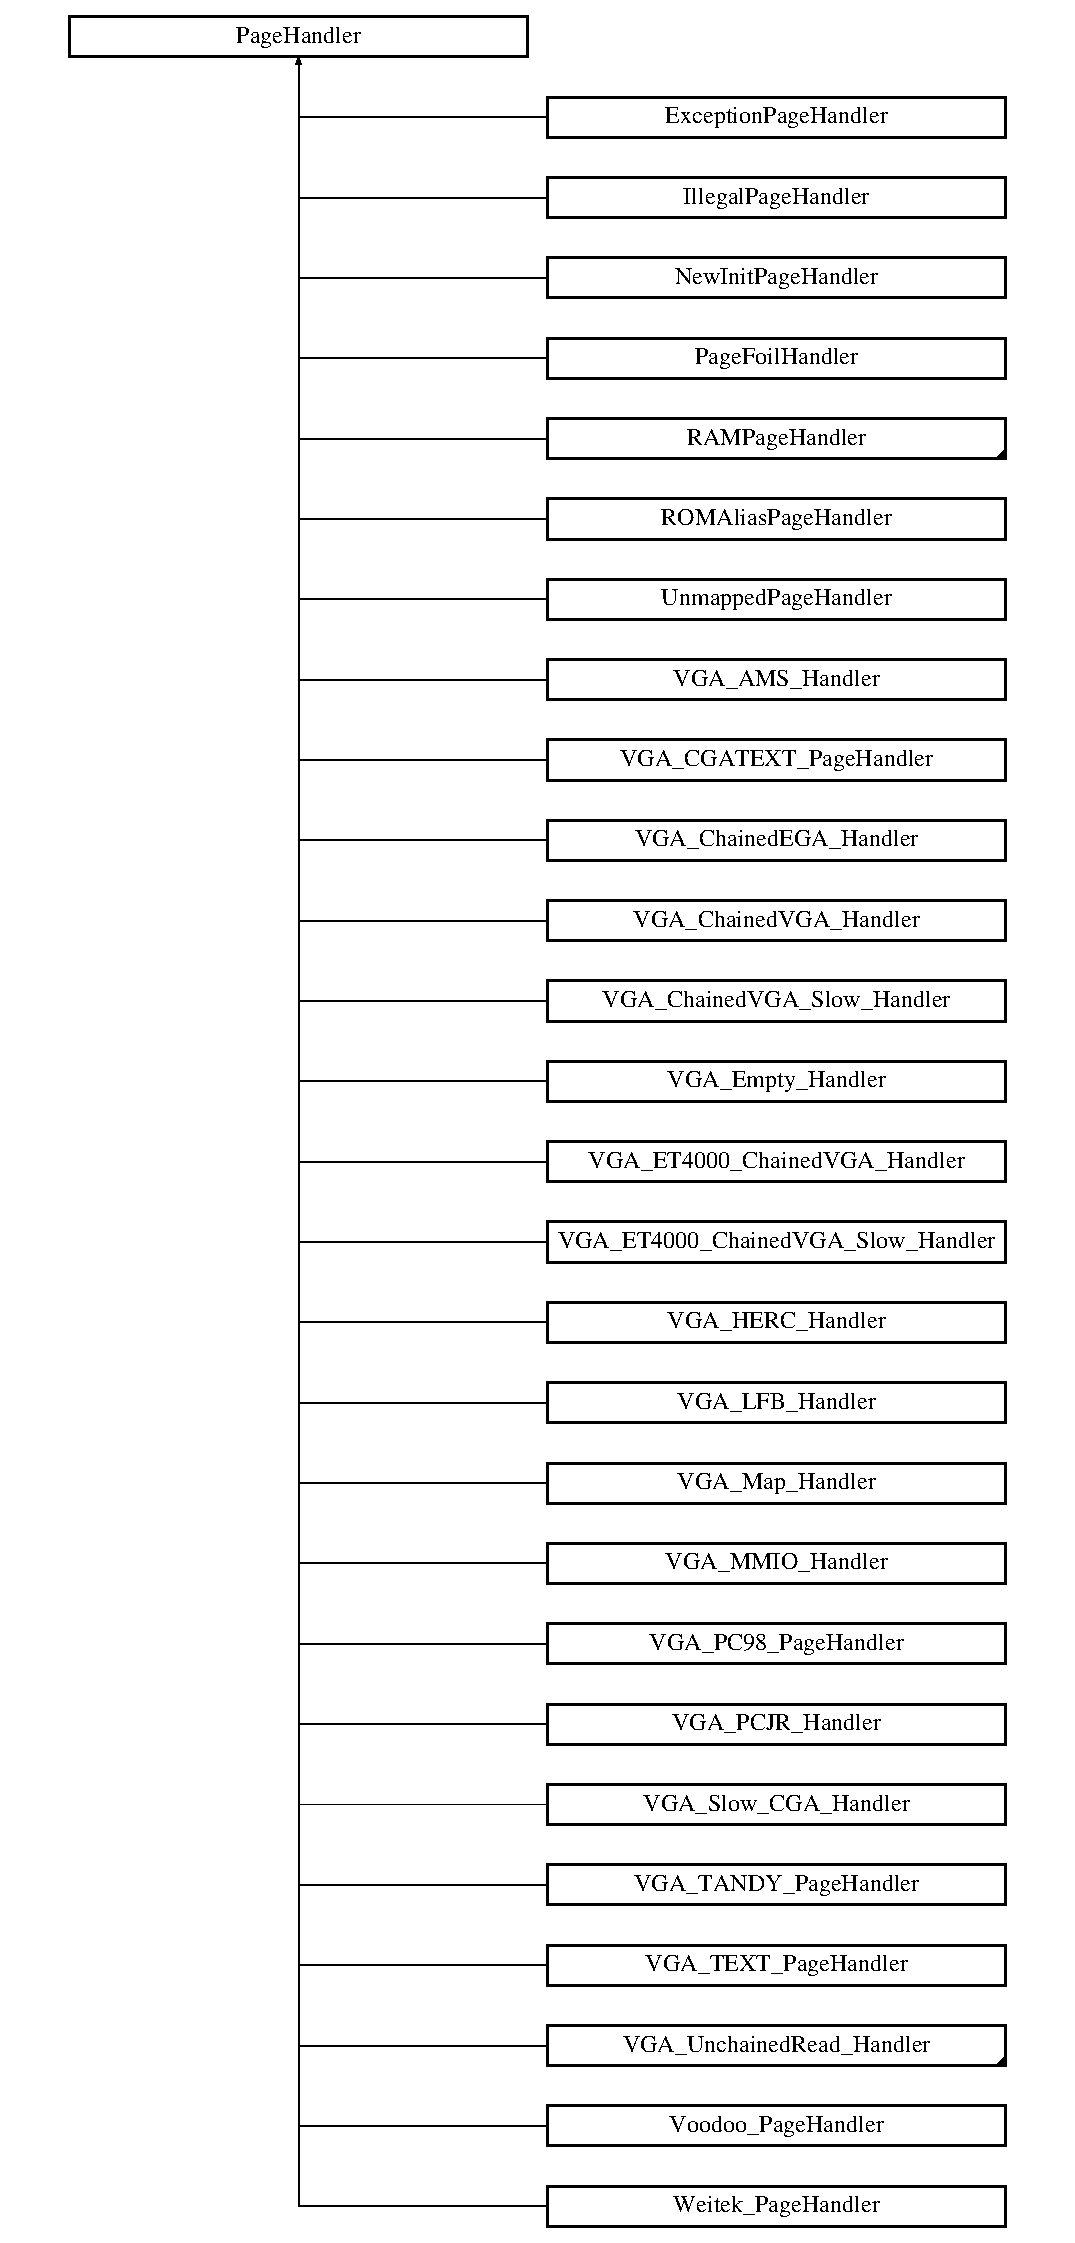
\includegraphics[height=12.000000cm]{classPageHandler}
\end{center}
\end{figure}
\subsection*{Public Member Functions}
\begin{DoxyCompactItemize}
\item 
\hypertarget{classPageHandler_a009efc4a2c49e562c8a0e0dca2bb91eb}{{\bfseries Page\-Handler} (Bitu flg)}\label{classPageHandler_a009efc4a2c49e562c8a0e0dca2bb91eb}

\item 
\hypertarget{classPageHandler_a741d1800da3de891f7e7d1ef921f92f5}{virtual Bitu {\bfseries readb} (Phys\-Pt addr)}\label{classPageHandler_a741d1800da3de891f7e7d1ef921f92f5}

\item 
\hypertarget{classPageHandler_a220266243629d1c0d4e1222be817471b}{virtual Bitu {\bfseries readw} (Phys\-Pt addr)}\label{classPageHandler_a220266243629d1c0d4e1222be817471b}

\item 
\hypertarget{classPageHandler_a0a0ee09fb7fface5af93f25d110d6661}{virtual Bitu {\bfseries readd} (Phys\-Pt addr)}\label{classPageHandler_a0a0ee09fb7fface5af93f25d110d6661}

\item 
\hypertarget{classPageHandler_aa848d57a4a20808815f179c9af8a44dc}{virtual void {\bfseries writeb} (Phys\-Pt addr, Bitu val)}\label{classPageHandler_aa848d57a4a20808815f179c9af8a44dc}

\item 
\hypertarget{classPageHandler_a297027c1a4430d5afe642a4ffaf04473}{virtual void {\bfseries writew} (Phys\-Pt addr, Bitu val)}\label{classPageHandler_a297027c1a4430d5afe642a4ffaf04473}

\item 
\hypertarget{classPageHandler_aebd9846b268b5844113039e60b564539}{virtual void {\bfseries writed} (Phys\-Pt addr, Bitu val)}\label{classPageHandler_aebd9846b268b5844113039e60b564539}

\item 
\hypertarget{classPageHandler_aec146fc4be69c0f37707c97aa1d9d7a2}{virtual Host\-Pt {\bfseries Get\-Host\-Read\-Pt} (Bitu phys\-\_\-page)}\label{classPageHandler_aec146fc4be69c0f37707c97aa1d9d7a2}

\item 
\hypertarget{classPageHandler_a9be437d29e87536d012d4520cb3ec52d}{virtual Host\-Pt {\bfseries Get\-Host\-Write\-Pt} (Bitu phys\-\_\-page)}\label{classPageHandler_a9be437d29e87536d012d4520cb3ec52d}

\item 
\hypertarget{classPageHandler_ae3dcf8d33fef258d08637cb0baf51a3d}{virtual bool {\bfseries readb\-\_\-checked} (Phys\-Pt addr, Bit8u $\ast$val)}\label{classPageHandler_ae3dcf8d33fef258d08637cb0baf51a3d}

\item 
\hypertarget{classPageHandler_a69bd6b5dd4e6c86211129df23045711a}{virtual bool {\bfseries readw\-\_\-checked} (Phys\-Pt addr, Bit16u $\ast$val)}\label{classPageHandler_a69bd6b5dd4e6c86211129df23045711a}

\item 
\hypertarget{classPageHandler_a8f2c1c323c5159348031ae6d7ca11718}{virtual bool {\bfseries readd\-\_\-checked} (Phys\-Pt addr, Bit32u $\ast$val)}\label{classPageHandler_a8f2c1c323c5159348031ae6d7ca11718}

\item 
\hypertarget{classPageHandler_a2e43caf55e0f752d080ef1e723533e8e}{virtual bool {\bfseries writeb\-\_\-checked} (Phys\-Pt addr, Bitu val)}\label{classPageHandler_a2e43caf55e0f752d080ef1e723533e8e}

\item 
\hypertarget{classPageHandler_a62c89d9498bbaa9e962d02f3ebdbbf64}{virtual bool {\bfseries writew\-\_\-checked} (Phys\-Pt addr, Bitu val)}\label{classPageHandler_a62c89d9498bbaa9e962d02f3ebdbbf64}

\item 
\hypertarget{classPageHandler_aab88a929a0647d9923ab75aaf62ce633}{virtual bool {\bfseries writed\-\_\-checked} (Phys\-Pt addr, Bitu val)}\label{classPageHandler_aab88a929a0647d9923ab75aaf62ce633}

\item 
\hypertarget{classPageHandler_a352d52997241c574d4ef7f12d842f697}{const Bitu {\bfseries get\-Flags} () const }\label{classPageHandler_a352d52997241c574d4ef7f12d842f697}

\item 
\hypertarget{classPageHandler_a14611a8cfa950d5305d074252189139a}{void {\bfseries set\-Flags} (Bitu flags\-New)}\label{classPageHandler_a14611a8cfa950d5305d074252189139a}

\end{DoxyCompactItemize}
\subsection*{Public Attributes}
\begin{DoxyCompactItemize}
\item 
\hypertarget{classPageHandler_afdba8b3717029016c4b530339a2440d3}{Bitu {\bfseries flags}}\label{classPageHandler_afdba8b3717029016c4b530339a2440d3}

\end{DoxyCompactItemize}


\subsection{Detailed Description}


Definition at line 89 of file paging.\-h.



The documentation for this class was generated from the following files\-:\begin{DoxyCompactItemize}
\item 
include/paging.\-h\item 
src/cpu/paging.\-cpp\end{DoxyCompactItemize}

\hypertarget{structPagingBlock}{\section{Paging\-Block Struct Reference}
\label{structPagingBlock}\index{Paging\-Block@{Paging\-Block}}
}
\subsection*{Public Attributes}
\begin{DoxyCompactItemize}
\item 
\hypertarget{structPagingBlock_a110f3f713ace59834f2f31983c1639cd}{Bitu {\bfseries cr3}}\label{structPagingBlock_a110f3f713ace59834f2f31983c1639cd}

\item 
\hypertarget{structPagingBlock_a9feb5924c8bb574637d86206e8a8f4b3}{Bitu {\bfseries cr2}}\label{structPagingBlock_a9feb5924c8bb574637d86206e8a8f4b3}

\item 
\hypertarget{structPagingBlock_a98edb6275607c408dc2078213632bf4e}{bool {\bfseries wp}}\label{structPagingBlock_a98edb6275607c408dc2078213632bf4e}

\item 
\hypertarget{structPagingBlock_a0fb1064bf4d86c09c4d7d87a9a239b8d}{\begin{tabbing}
xx\=xx\=xx\=xx\=xx\=xx\=xx\=xx\=xx\=\kill
struct \{\\
\>Bitu {\bfseries page}\\
\>PhysPt {\bfseries addr}\\
\} {\bfseries base}}\label{structPagingBlock_a0fb1064bf4d86c09c4d7d87a9a239b8d}
\\

\end{tabbing}\item 
\hypertarget{structPagingBlock_abeb868a31825b42e2ae5bb956aa92252}{\begin{tabbing}
xx\=xx\=xx\=xx\=xx\=xx\=xx\=xx\=xx\=\kill
struct \{\\
\>HostPt {\bfseries read} \mbox{[}TLB\_SIZE\mbox{]}\\
\>HostPt {\bfseries write} \mbox{[}TLB\_SIZE\mbox{]}\\
\>\hyperlink{classPageHandler}{PageHandler} $\ast$ {\bfseries readhandler} \mbox{[}TLB\_SIZE\mbox{]}\\
\>\hyperlink{classPageHandler}{PageHandler} $\ast$ {\bfseries writehandler} \mbox{[}TLB\_SIZE\mbox{]}\\
\>Bit32u {\bfseries phys\_page} \mbox{[}TLB\_SIZE\mbox{]}\\
\} {\bfseries tlb}}\label{structPagingBlock_abeb868a31825b42e2ae5bb956aa92252}
\\

\end{tabbing}\item 
\hypertarget{structPagingBlock_a7ef334d16f2fcdc4c2108e76e7dc9ff7}{\begin{tabbing}
xx\=xx\=xx\=xx\=xx\=xx\=xx\=xx\=xx\=\kill
struct \{\\
\>Bitu {\bfseries used}\\
\>Bit32u {\bfseries entries} \mbox{[}PAGING\_LINKS\mbox{]}\\
\} {\bfseries links}}\label{structPagingBlock_a7ef334d16f2fcdc4c2108e76e7dc9ff7}
\\

\end{tabbing}\item 
\hypertarget{structPagingBlock_a7b6a29b0e21185cc60024ae354359d90}{\begin{tabbing}
xx\=xx\=xx\=xx\=xx\=xx\=xx\=xx\=xx\=\kill
struct \{\\
\>Bitu {\bfseries used}\\
\>Bit32u {\bfseries entries} \mbox{[}PAGING\_LINKS\mbox{]}\\
\} {\bfseries ur\_links}}\label{structPagingBlock_a7b6a29b0e21185cc60024ae354359d90}
\\

\end{tabbing}\item 
\hypertarget{structPagingBlock_ad275dca9e1641d9936cf106a71d5abf2}{\begin{tabbing}
xx\=xx\=xx\=xx\=xx\=xx\=xx\=xx\=xx\=\kill
struct \{\\
\>Bitu {\bfseries used}\\
\>Bit32u {\bfseries entries} \mbox{[}PAGING\_LINKS\mbox{]}\\
\} {\bfseries krw\_links}}\label{structPagingBlock_ad275dca9e1641d9936cf106a71d5abf2}
\\

\end{tabbing}\item 
\hypertarget{structPagingBlock_ab7bba3ffdb2eed80d46da43ab89e844e}{\begin{tabbing}
xx\=xx\=xx\=xx\=xx\=xx\=xx\=xx\=xx\=\kill
struct \{\\
\>Bitu {\bfseries used}\\
\>Bit32u {\bfseries entries} \mbox{[}PAGING\_LINKS\mbox{]}\\
\} {\bfseries kr\_links}}\label{structPagingBlock_ab7bba3ffdb2eed80d46da43ab89e844e}
\\

\end{tabbing}\item 
\hypertarget{structPagingBlock_a0f959a5a804ec18582f09350156f3e4f}{Bit32u {\bfseries firstmb} \mbox{[}L\-I\-N\-K\-\_\-\-S\-T\-A\-R\-T\mbox{]}}\label{structPagingBlock_a0f959a5a804ec18582f09350156f3e4f}

\item 
\hypertarget{structPagingBlock_a24a172f80cdcd97ec729fc564873831f}{bool {\bfseries enabled}}\label{structPagingBlock_a24a172f80cdcd97ec729fc564873831f}

\end{DoxyCompactItemize}


\subsection{Detailed Description}


Definition at line 266 of file paging.\-h.



The documentation for this struct was generated from the following file\-:\begin{DoxyCompactItemize}
\item 
include/paging.\-h\end{DoxyCompactItemize}

\hypertarget{structPC98__GDC__state}{\section{P\-C98\-\_\-\-G\-D\-C\-\_\-state Struct Reference}
\label{structPC98__GDC__state}\index{P\-C98\-\_\-\-G\-D\-C\-\_\-state@{P\-C98\-\_\-\-G\-D\-C\-\_\-state}}
}
\subsection*{Public Member Functions}
\begin{DoxyCompactItemize}
\item 
\hypertarget{structPC98__GDC__state_a7973469db8c58471cd105cc5f2513bb1}{void {\bfseries reset\-\_\-fifo} (void)}\label{structPC98__GDC__state_a7973469db8c58471cd105cc5f2513bb1}

\item 
\hypertarget{structPC98__GDC__state_a4836b9d30ad97c0d491c628c493a31a3}{void {\bfseries reset\-\_\-rfifo} (void)}\label{structPC98__GDC__state_a4836b9d30ad97c0d491c628c493a31a3}

\item 
\hypertarget{structPC98__GDC__state_a0eab727dd82dfad6c340daaa337f442d}{void {\bfseries flush\-\_\-fifo\-\_\-old} (void)}\label{structPC98__GDC__state_a0eab727dd82dfad6c340daaa337f442d}

\item 
\hypertarget{structPC98__GDC__state_af404e360236ebfe30003bd00761e7eb1}{bool {\bfseries write\-\_\-fifo} (const uint16\-\_\-t c)}\label{structPC98__GDC__state_af404e360236ebfe30003bd00761e7eb1}

\item 
\hypertarget{structPC98__GDC__state_a19867db16d1d33edb3cec74c9c8596cd}{bool {\bfseries write\-\_\-fifo\-\_\-command} (const unsigned char c)}\label{structPC98__GDC__state_a19867db16d1d33edb3cec74c9c8596cd}

\item 
\hypertarget{structPC98__GDC__state_aedfc62f64c943388975adedbc30458bf}{bool {\bfseries write\-\_\-fifo\-\_\-param} (const unsigned char c)}\label{structPC98__GDC__state_aedfc62f64c943388975adedbc30458bf}

\item 
\hypertarget{structPC98__GDC__state_ad34b46692e4fe7b2bc059509a5b465af}{bool {\bfseries rfifo\-\_\-has\-\_\-content} (void)}\label{structPC98__GDC__state_ad34b46692e4fe7b2bc059509a5b465af}

\item 
\hypertarget{structPC98__GDC__state_af5efa59d1f87f1a172c4fd86e0367ab0}{uint8\-\_\-t {\bfseries read\-\_\-status} (void)}\label{structPC98__GDC__state_af5efa59d1f87f1a172c4fd86e0367ab0}

\item 
\hypertarget{structPC98__GDC__state_a7d6b362a6b895d3a1e7636de691e0e00}{uint8\-\_\-t {\bfseries rfifo\-\_\-read\-\_\-data} (void)}\label{structPC98__GDC__state_a7d6b362a6b895d3a1e7636de691e0e00}

\item 
\hypertarget{structPC98__GDC__state_a0ccae08dcb56ec0101cc2d4cfd157eb1}{void {\bfseries idle\-\_\-proc} (void)}\label{structPC98__GDC__state_a0ccae08dcb56ec0101cc2d4cfd157eb1}

\item 
\hypertarget{structPC98__GDC__state_ae84ccc228e028cda626d6daf99f87838}{void {\bfseries force\-\_\-fifo\-\_\-complete} (void)}\label{structPC98__GDC__state_ae84ccc228e028cda626d6daf99f87838}

\item 
\hypertarget{structPC98__GDC__state_a6ba4e40ce3639a48cfbadba1872df0d0}{void {\bfseries take\-\_\-cursor\-\_\-char\-\_\-setup} (unsigned char bi)}\label{structPC98__GDC__state_a6ba4e40ce3639a48cfbadba1872df0d0}

\item 
\hypertarget{structPC98__GDC__state_a80e0ea7ab57f9fc28dd8bd1f50d71be1}{void {\bfseries take\-\_\-cursor\-\_\-pos} (unsigned char bi)}\label{structPC98__GDC__state_a80e0ea7ab57f9fc28dd8bd1f50d71be1}

\item 
\hypertarget{structPC98__GDC__state_af2b09ec20b24e73d7db449705d1f2ec8}{void {\bfseries take\-\_\-reset\-\_\-sync\-\_\-parameters} (void)}\label{structPC98__GDC__state_af2b09ec20b24e73d7db449705d1f2ec8}

\item 
\hypertarget{structPC98__GDC__state_a391cd10c2a662e20d413727c48000af3}{void {\bfseries cursor\-\_\-advance} (void)}\label{structPC98__GDC__state_a391cd10c2a662e20d413727c48000af3}

\item 
\hypertarget{structPC98__GDC__state_ac85b9bb3a3bbd0b4f66de944483d8424}{void {\bfseries begin\-\_\-frame} (void)}\label{structPC98__GDC__state_ac85b9bb3a3bbd0b4f66de944483d8424}

\item 
\hypertarget{structPC98__GDC__state_ab65b859c51a1a67e418519493d965cf2}{void {\bfseries next\-\_\-line} (void)}\label{structPC98__GDC__state_ab65b859c51a1a67e418519493d965cf2}

\item 
\hypertarget{structPC98__GDC__state_abda2457b69d686010fc4f31761c06a67}{void {\bfseries load\-\_\-display\-\_\-partition} (void)}\label{structPC98__GDC__state_abda2457b69d686010fc4f31761c06a67}

\item 
\hypertarget{structPC98__GDC__state_a06ff5284e20626e39d26f2aa35e9b5a0}{void {\bfseries next\-\_\-display\-\_\-partition} (void)}\label{structPC98__GDC__state_a06ff5284e20626e39d26f2aa35e9b5a0}

\item 
\hypertarget{structPC98__GDC__state_ad618c0a11e12648f00e355b1b2f35242}{size\-\_\-t {\bfseries fifo\-\_\-can\-\_\-read} (void)}\label{structPC98__GDC__state_ad618c0a11e12648f00e355b1b2f35242}

\item 
\hypertarget{structPC98__GDC__state_ac796dca290c0a392dee75bae6c5baf97}{bool {\bfseries fifo\-\_\-empty} (void)}\label{structPC98__GDC__state_ac796dca290c0a392dee75bae6c5baf97}

\item 
\hypertarget{structPC98__GDC__state_abeb2e59a5f11da4c37419d7cbdde7d4f}{Bit16u {\bfseries read\-\_\-fifo} (void)}\label{structPC98__GDC__state_abeb2e59a5f11da4c37419d7cbdde7d4f}

\end{DoxyCompactItemize}
\subsection*{Public Attributes}
\begin{DoxyCompactItemize}
\item 
\hypertarget{structPC98__GDC__state_ad53f1416505372b98977b8648c0b343b}{uint8\-\_\-t {\bfseries cmd\-\_\-parm\-\_\-tmp} \mbox{[}8\mbox{]}}\label{structPC98__GDC__state_ad53f1416505372b98977b8648c0b343b}

\item 
\hypertarget{structPC98__GDC__state_ad75c87326eb9d59df669ce4b7ea1100f}{uint8\-\_\-t {\bfseries rfifo} \mbox{[}P\-C98\-\_\-\-G\-D\-C\-\_\-\-F\-I\-F\-O\-\_\-\-S\-I\-Z\-E\mbox{]}}\label{structPC98__GDC__state_ad75c87326eb9d59df669ce4b7ea1100f}

\item 
\hypertarget{structPC98__GDC__state_aaa41b9c1f0b095f406aa564819aff26e}{uint8\-\_\-t {\bfseries rfifo\-\_\-read}}\label{structPC98__GDC__state_aaa41b9c1f0b095f406aa564819aff26e}

\item 
\hypertarget{structPC98__GDC__state_abfd13e784549ab4f9c859e1034ee41be}{uint8\-\_\-t {\bfseries rfifo\-\_\-write}}\label{structPC98__GDC__state_abfd13e784549ab4f9c859e1034ee41be}

\item 
\hypertarget{structPC98__GDC__state_ad64a8fd6f8d03081289691c29f96ded2}{uint16\-\_\-t {\bfseries fifo} \mbox{[}P\-C98\-\_\-\-G\-D\-C\-\_\-\-F\-I\-F\-O\-\_\-\-S\-I\-Z\-E\mbox{]}}\label{structPC98__GDC__state_ad64a8fd6f8d03081289691c29f96ded2}

\item 
\hypertarget{structPC98__GDC__state_a0829cda4d6f604233d94412231b1278c}{uint8\-\_\-t {\bfseries fifo\-\_\-read}}\label{structPC98__GDC__state_a0829cda4d6f604233d94412231b1278c}

\item 
\hypertarget{structPC98__GDC__state_a7d5646ae4fd268954e381dba35ac65d8}{uint8\-\_\-t {\bfseries fifo\-\_\-write}}\label{structPC98__GDC__state_a7d5646ae4fd268954e381dba35ac65d8}

\item 
\hypertarget{structPC98__GDC__state_a751d643e886af813597e85c821d9f8fd}{uint8\-\_\-t {\bfseries param\-\_\-ram} \mbox{[}16\mbox{]}}\label{structPC98__GDC__state_a751d643e886af813597e85c821d9f8fd}

\item 
\hypertarget{structPC98__GDC__state_ad0af657355ec1875c72313f3e24841d4}{uint8\-\_\-t {\bfseries param\-\_\-ram\-\_\-wptr}}\label{structPC98__GDC__state_ad0af657355ec1875c72313f3e24841d4}

\item 
\hypertarget{structPC98__GDC__state_a654e9a32973bd64bf883d497bc2a8431}{uint16\-\_\-t {\bfseries scan\-\_\-address}}\label{structPC98__GDC__state_a654e9a32973bd64bf883d497bc2a8431}

\item 
\hypertarget{structPC98__GDC__state_adbba69a00d55ac29528a9656aeae90c5}{uint8\-\_\-t {\bfseries row\-\_\-height}}\label{structPC98__GDC__state_adbba69a00d55ac29528a9656aeae90c5}

\item 
\hypertarget{structPC98__GDC__state_a3ab8bbf49d9e8efca947afa03cd77bc9}{uint8\-\_\-t {\bfseries row\-\_\-line}}\label{structPC98__GDC__state_a3ab8bbf49d9e8efca947afa03cd77bc9}

\item 
\hypertarget{structPC98__GDC__state_a9ef7dbeccbb9a9c915b0c020d6e3290e}{uint8\-\_\-t {\bfseries display\-\_\-partition}}\label{structPC98__GDC__state_a9ef7dbeccbb9a9c915b0c020d6e3290e}

\item 
\hypertarget{structPC98__GDC__state_ad71b8aec898372d6913ad66e3ce17f19}{uint16\-\_\-t {\bfseries display\-\_\-partition\-\_\-rem\-\_\-lines}}\label{structPC98__GDC__state_ad71b8aec898372d6913ad66e3ce17f19}

\item 
\hypertarget{structPC98__GDC__state_a57cc8033233ce0efec486e96b3c9e52b}{uint8\-\_\-t {\bfseries display\-\_\-partition\-\_\-mask}}\label{structPC98__GDC__state_a57cc8033233ce0efec486e96b3c9e52b}

\item 
\hypertarget{structPC98__GDC__state_a5d8da8d74cac150e8fc674d006c894cf}{uint16\-\_\-t {\bfseries active\-\_\-display\-\_\-lines}}\label{structPC98__GDC__state_a5d8da8d74cac150e8fc674d006c894cf}

\item 
\hypertarget{structPC98__GDC__state_a37d15232d351276cbf58d1db56699e2c}{uint16\-\_\-t {\bfseries active\-\_\-display\-\_\-words\-\_\-per\-\_\-line}}\label{structPC98__GDC__state_a37d15232d351276cbf58d1db56699e2c}

\item 
\hypertarget{structPC98__GDC__state_a0546c8864db0e1b4565e983409dadcd7}{uint16\-\_\-t {\bfseries display\-\_\-pitch}}\label{structPC98__GDC__state_a0546c8864db0e1b4565e983409dadcd7}

\item 
\hypertarget{structPC98__GDC__state_a42abdf51ea59faac4bb55e86500d627f}{uint8\-\_\-t {\bfseries horizontal\-\_\-sync\-\_\-width}}\label{structPC98__GDC__state_a42abdf51ea59faac4bb55e86500d627f}

\item 
\hypertarget{structPC98__GDC__state_a528d52a66abb61859d8d866463b0ddba}{uint8\-\_\-t {\bfseries vertical\-\_\-sync\-\_\-width}}\label{structPC98__GDC__state_a528d52a66abb61859d8d866463b0ddba}

\item 
\hypertarget{structPC98__GDC__state_a8a30c42b0ec0187669fd62bb8e5ee1fd}{uint8\-\_\-t {\bfseries horizontal\-\_\-front\-\_\-porch\-\_\-width}}\label{structPC98__GDC__state_a8a30c42b0ec0187669fd62bb8e5ee1fd}

\item 
\hypertarget{structPC98__GDC__state_afed5fbe810687a114231165d2035320f}{uint8\-\_\-t {\bfseries horizontal\-\_\-back\-\_\-porch\-\_\-width}}\label{structPC98__GDC__state_afed5fbe810687a114231165d2035320f}

\item 
\hypertarget{structPC98__GDC__state_a09d208aa4df7a0aa802695c76e55e84d}{uint8\-\_\-t {\bfseries vertical\-\_\-front\-\_\-porch\-\_\-width}}\label{structPC98__GDC__state_a09d208aa4df7a0aa802695c76e55e84d}

\item 
\hypertarget{structPC98__GDC__state_ae2979bda1db66e6cd96a9374f50c8460}{uint8\-\_\-t {\bfseries vertical\-\_\-back\-\_\-porch\-\_\-width}}\label{structPC98__GDC__state_ae2979bda1db66e6cd96a9374f50c8460}

\item 
\hypertarget{structPC98__GDC__state_afeee708ec68e7b11dfb018eef6112a4a}{uint8\-\_\-t {\bfseries display\-\_\-mode}}\label{structPC98__GDC__state_afeee708ec68e7b11dfb018eef6112a4a}

\item 
\hypertarget{structPC98__GDC__state_a58177cd0a41ec852d53db1d668420089}{uint8\-\_\-t {\bfseries video\-\_\-framing}}\label{structPC98__GDC__state_a58177cd0a41ec852d53db1d668420089}

\item 
\hypertarget{structPC98__GDC__state_aff0017111dc87de5612eb90cc4f60e78}{uint8\-\_\-t {\bfseries current\-\_\-command}}\label{structPC98__GDC__state_aff0017111dc87de5612eb90cc4f60e78}

\item 
\hypertarget{structPC98__GDC__state_a510fb5f8bab0480ad0862a28bcbaa38b}{uint8\-\_\-t {\bfseries proc\-\_\-step}}\label{structPC98__GDC__state_a510fb5f8bab0480ad0862a28bcbaa38b}

\item 
\hypertarget{structPC98__GDC__state_aac0268546867b0e7cac68aa263afdace}{uint8\-\_\-t {\bfseries cursor\-\_\-blink\-\_\-state}}\label{structPC98__GDC__state_aac0268546867b0e7cac68aa263afdace}

\item 
\hypertarget{structPC98__GDC__state_aebd7aff24bf501c09a83521de8bc756b}{uint8\-\_\-t {\bfseries cursor\-\_\-blink\-\_\-count}}\label{structPC98__GDC__state_aebd7aff24bf501c09a83521de8bc756b}

\item 
\hypertarget{structPC98__GDC__state_a1da10b2642246d1e4315b301f91b816f}{uint8\-\_\-t {\bfseries cursor\-\_\-blink\-\_\-rate}}\label{structPC98__GDC__state_a1da10b2642246d1e4315b301f91b816f}

\item 
\hypertarget{structPC98__GDC__state_a30fc555b9d29ee7b94597c134903fa1a}{bool {\bfseries draw\-\_\-only\-\_\-during\-\_\-retrace}}\label{structPC98__GDC__state_a30fc555b9d29ee7b94597c134903fa1a}

\item 
\hypertarget{structPC98__GDC__state_ab2e743dbada1318967bd10505bcfae33}{bool {\bfseries dynamic\-\_\-ram\-\_\-refresh}}\label{structPC98__GDC__state_ab2e743dbada1318967bd10505bcfae33}

\item 
\hypertarget{structPC98__GDC__state_a2f82a64dee33666f051f2358b39b36e1}{bool {\bfseries master\-\_\-sync}}\label{structPC98__GDC__state_a2f82a64dee33666f051f2358b39b36e1}

\item 
\hypertarget{structPC98__GDC__state_a6d8c34e7786906c0bf3a71a8223b47c7}{bool {\bfseries display\-\_\-enable}}\label{structPC98__GDC__state_a6d8c34e7786906c0bf3a71a8223b47c7}

\item 
\hypertarget{structPC98__GDC__state_a2d974909bf478b470db46d7a391d45be}{bool {\bfseries cursor\-\_\-enable}}\label{structPC98__GDC__state_a2d974909bf478b470db46d7a391d45be}

\item 
\hypertarget{structPC98__GDC__state_a052103fb7ab862c6087ca893f42b1889}{bool {\bfseries cursor\-\_\-blink}}\label{structPC98__GDC__state_a052103fb7ab862c6087ca893f42b1889}

\item 
\hypertarget{structPC98__GDC__state_ace0fcb3c221beebe98c51e49be38bb2f}{bool {\bfseries idle}}\label{structPC98__GDC__state_ace0fcb3c221beebe98c51e49be38bb2f}

\item 
\hypertarget{structPC98__GDC__state_a38abe8d027dbbe87e2abeda97a7b1ebb}{bool {\bfseries doublescan}}\label{structPC98__GDC__state_a38abe8d027dbbe87e2abeda97a7b1ebb}

\end{DoxyCompactItemize}


\subsection{Detailed Description}


Definition at line 32 of file pc98\-\_\-gdc.\-h.



The documentation for this struct was generated from the following file\-:\begin{DoxyCompactItemize}
\item 
include/pc98\-\_\-gdc.\-h\end{DoxyCompactItemize}

\hypertarget{unionpc98__tile}{\section{pc98\-\_\-tile Union Reference}
\label{unionpc98__tile}\index{pc98\-\_\-tile@{pc98\-\_\-tile}}
}
\subsection*{Public Attributes}
\begin{DoxyCompactItemize}
\item 
\hypertarget{unionpc98__tile_a1d4e5b3d3509eefc0a5f4a11d8bdea5b}{uint8\-\_\-t {\bfseries b} \mbox{[}2\mbox{]}}\label{unionpc98__tile_a1d4e5b3d3509eefc0a5f4a11d8bdea5b}

\item 
\hypertarget{unionpc98__tile_aeb46ba0689f1df876b1c4ccd8f77a022}{uint16\-\_\-t {\bfseries w}}\label{unionpc98__tile_aeb46ba0689f1df876b1c4ccd8f77a022}

\end{DoxyCompactItemize}


\subsection{Detailed Description}


Definition at line 27 of file pc98\-\_\-gdc.\-h.



The documentation for this union was generated from the following file\-:\begin{DoxyCompactItemize}
\item 
include/pc98\-\_\-gdc.\-h\end{DoxyCompactItemize}

\hypertarget{classPCI__Device}{\section{P\-C\-I\-\_\-\-Device Class Reference}
\label{classPCI__Device}\index{P\-C\-I\-\_\-\-Device@{P\-C\-I\-\_\-\-Device}}
}
Inheritance diagram for P\-C\-I\-\_\-\-Device\-:\begin{figure}[H]
\begin{center}
\leavevmode
\includegraphics[height=2.000000cm]{classPCI__Device}
\end{center}
\end{figure}
\subsection*{Public Member Functions}
\begin{DoxyCompactItemize}
\item 
\hypertarget{classPCI__Device_a3e88023ba031fe2137b1b83307d10139}{{\bfseries P\-C\-I\-\_\-\-Device} (Bit16u vendor, Bit16u device)}\label{classPCI__Device_a3e88023ba031fe2137b1b83307d10139}

\item 
\hypertarget{classPCI__Device_aeffcee3f3604817e13621fd0af3c116c}{Bit16u {\bfseries get\-Device\-I\-D} ()}\label{classPCI__Device_aeffcee3f3604817e13621fd0af3c116c}

\item 
\hypertarget{classPCI__Device_ae301eac6564171b8ebd631f1f5a5b010}{void {\bfseries set\-Device\-I\-D} (const Bit16u device)}\label{classPCI__Device_ae301eac6564171b8ebd631f1f5a5b010}

\item 
\hypertarget{classPCI__Device_a250d9180675cc1d1b95c9c3bbb98cbc6}{Bit16u {\bfseries get\-Vendor\-I\-D} ()}\label{classPCI__Device_a250d9180675cc1d1b95c9c3bbb98cbc6}

\item 
\hypertarget{classPCI__Device_a77e5dc350044cbcf1d4282bd0960e29f}{void {\bfseries set\-Vendor\-I\-D} (const Bit16u vendor)}\label{classPCI__Device_a77e5dc350044cbcf1d4282bd0960e29f}

\item 
\hypertarget{classPCI__Device_a61dff5e6d0d2a159eb85c7fdbab85544}{virtual void {\bfseries config\-\_\-write} (Bit8u regnum, Bitu iolen, Bit32u value)}\label{classPCI__Device_a61dff5e6d0d2a159eb85c7fdbab85544}

\item 
\hypertarget{classPCI__Device_aa3b02b458e4c1907f654e34166f0cb81}{virtual Bit32u {\bfseries config\-\_\-read} (Bit8u regnum, Bitu iolen)}\label{classPCI__Device_aa3b02b458e4c1907f654e34166f0cb81}

\end{DoxyCompactItemize}
\subsection*{Public Attributes}
\begin{DoxyCompactItemize}
\item 
\hypertarget{classPCI__Device_a96714f926af98bbc3ae6030b918e4371}{unsigned char {\bfseries config} \mbox{[}256\mbox{]}}\label{classPCI__Device_a96714f926af98bbc3ae6030b918e4371}

\item 
\hypertarget{classPCI__Device_a0dc5ffb8e062148eb946488cfdf9b2fc}{unsigned char {\bfseries config\-\_\-writemask} \mbox{[}256\mbox{]}}\label{classPCI__Device_a0dc5ffb8e062148eb946488cfdf9b2fc}

\end{DoxyCompactItemize}


\subsection{Detailed Description}


Definition at line 26 of file pci\-\_\-bus.\-h.



The documentation for this class was generated from the following files\-:\begin{DoxyCompactItemize}
\item 
include/pci\-\_\-bus.\-h\item 
src/hardware/pci\-\_\-bus.\-cpp\end{DoxyCompactItemize}

\hypertarget{classProgram}{\section{Program Class Reference}
\label{classProgram}\index{Program@{Program}}
}
Inheritance diagram for Program\-:\begin{figure}[H]
\begin{center}
\leavevmode
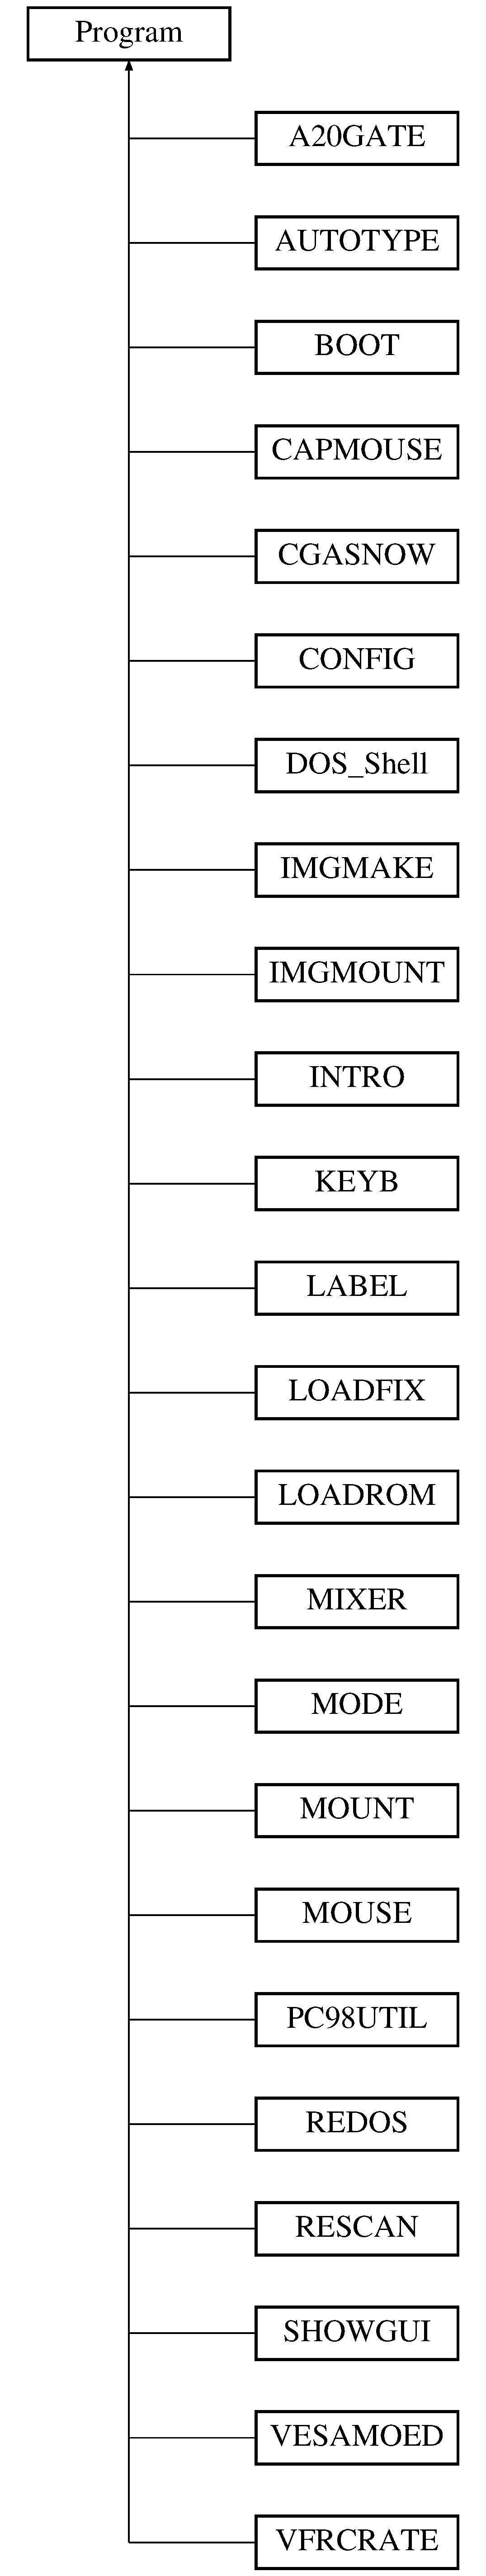
\includegraphics[height=2.000000cm]{classProgram}
\end{center}
\end{figure}
\subsection*{Public Member Functions}
\begin{DoxyCompactItemize}
\item 
\hypertarget{classProgram_acd37c94c3c12a55650a05ee1449aa176}{virtual void {\bfseries Run} (void)=0}\label{classProgram_acd37c94c3c12a55650a05ee1449aa176}

\item 
\hypertarget{classProgram_a0012adb877f24b04d836a37ab48f2c60}{bool {\bfseries Get\-Env\-Str} (const char $\ast$entry, std\-::string \&result)}\label{classProgram_a0012adb877f24b04d836a37ab48f2c60}

\item 
\hypertarget{classProgram_a58d316ec88ff44eff5188f46ef7eefd8}{bool {\bfseries Get\-Env\-Num} (Bitu num, std\-::string \&result)}\label{classProgram_a58d316ec88ff44eff5188f46ef7eefd8}

\item 
\hypertarget{classProgram_a67b647d573493de3f7237fe075a8532d}{Bitu {\bfseries Get\-Env\-Count} (void)}\label{classProgram_a67b647d573493de3f7237fe075a8532d}

\item 
\hypertarget{classProgram_a8a7d72f5c08f644fb19e5f36dc1c3d46}{bool {\bfseries Set\-Env} (const char $\ast$entry, const char $\ast$new\-\_\-string)}\label{classProgram_a8a7d72f5c08f644fb19e5f36dc1c3d46}

\item 
\hypertarget{classProgram_af3326c2431db683c8cbfcf1a4eb06f71}{void {\bfseries Write\-Out} (const char $\ast$format,...)}\label{classProgram_af3326c2431db683c8cbfcf1a4eb06f71}

\item 
\hypertarget{classProgram_aa45498c7e07ec784b72ed166ab69a847}{void {\bfseries Write\-Out\-\_\-\-No\-Parsing} (const char $\ast$format)}\label{classProgram_aa45498c7e07ec784b72ed166ab69a847}

\item 
\hypertarget{classProgram_a3b124865b50f681fa1d5ae05d71107f8}{void {\bfseries Change\-To\-Long\-Cmd} ()}\label{classProgram_a3b124865b50f681fa1d5ae05d71107f8}

\item 
\hypertarget{classProgram_a7a253f9ce31472b4b5c38791524f3ba8}{void {\bfseries Debug\-Dump\-Env} ()}\label{classProgram_a7a253f9ce31472b4b5c38791524f3ba8}

\item 
\hypertarget{classProgram_ab1fa236943ef14b02c59bc4225d216a1}{void {\bfseries Write\-Exit\-Status} ()}\label{classProgram_ab1fa236943ef14b02c59bc4225d216a1}

\end{DoxyCompactItemize}
\subsection*{Public Attributes}
\begin{DoxyCompactItemize}
\item 
\hypertarget{classProgram_a9e1bb1fc1b315bf697fb1872d6defe12}{unsigned char {\bfseries exit\-\_\-status}}\label{classProgram_a9e1bb1fc1b315bf697fb1872d6defe12}

\item 
\hypertarget{classProgram_ade1241ef2184833339588494094f7d4f}{std\-::string {\bfseries temp\-\_\-line}}\label{classProgram_ade1241ef2184833339588494094f7d4f}

\item 
\hypertarget{classProgram_af637f18e9637b148fbecbd3f0bc748fc}{\hyperlink{classCommandLine}{Command\-Line} $\ast$ {\bfseries cmd}}\label{classProgram_af637f18e9637b148fbecbd3f0bc748fc}

\item 
\hypertarget{classProgram_af2f99e812360b3748ec790f4e4023fc4}{\hyperlink{classDOS__PSP}{D\-O\-S\-\_\-\-P\-S\-P} $\ast$ {\bfseries psp}}\label{classProgram_af2f99e812360b3748ec790f4e4023fc4}

\end{DoxyCompactItemize}


\subsection{Detailed Description}


Definition at line 90 of file programs.\-h.



The documentation for this class was generated from the following file\-:\begin{DoxyCompactItemize}
\item 
include/programs.\-h\end{DoxyCompactItemize}

\hypertarget{classProp__bool}{\section{Prop\-\_\-bool Class Reference}
\label{classProp__bool}\index{Prop\-\_\-bool@{Prop\-\_\-bool}}
}
Inheritance diagram for Prop\-\_\-bool\-:\begin{figure}[H]
\begin{center}
\leavevmode
\includegraphics[height=2.000000cm]{classProp__bool}
\end{center}
\end{figure}
\subsection*{Public Member Functions}
\begin{DoxyCompactItemize}
\item 
\hypertarget{classProp__bool_ab70b5efc7550776962b20ecc1fd329ca}{{\bfseries Prop\-\_\-bool} (std\-::string const \&\-\_\-propname, Changeable\-::\-Value when, bool \-\_\-value)}\label{classProp__bool_ab70b5efc7550776962b20ecc1fd329ca}

\item 
\hypertarget{classProp__bool_a3027dcac0a1334e6b6912d99902b0b26}{bool {\bfseries Set\-Value} (std\-::string const \&input)}\label{classProp__bool_a3027dcac0a1334e6b6912d99902b0b26}

\end{DoxyCompactItemize}


\subsection{Detailed Description}


Definition at line 207 of file setup.\-h.



The documentation for this class was generated from the following files\-:\begin{DoxyCompactItemize}
\item 
include/setup.\-h\item 
src/misc/setup.\-cpp\end{DoxyCompactItemize}

\hypertarget{classProp__double}{\section{Prop\-\_\-double Class Reference}
\label{classProp__double}\index{Prop\-\_\-double@{Prop\-\_\-double}}
}
Inheritance diagram for Prop\-\_\-double\-:\begin{figure}[H]
\begin{center}
\leavevmode
\includegraphics[height=2.000000cm]{classProp__double}
\end{center}
\end{figure}
\subsection*{Public Member Functions}
\begin{DoxyCompactItemize}
\item 
\hypertarget{classProp__double_aa0facf6624ff88ee5d29fd70c5245ae9}{{\bfseries Prop\-\_\-double} (std\-::string const \&\-\_\-propname, Changeable\-::\-Value when, double \-\_\-value)}\label{classProp__double_aa0facf6624ff88ee5d29fd70c5245ae9}

\item 
\hypertarget{classProp__double_a29d1175964f35a4aa6b5e482e3dfdf00}{bool {\bfseries Set\-Value} (std\-::string const \&input)}\label{classProp__double_a29d1175964f35a4aa6b5e482e3dfdf00}

\end{DoxyCompactItemize}


\subsection{Detailed Description}


Definition at line 179 of file setup.\-h.



The documentation for this class was generated from the following files\-:\begin{DoxyCompactItemize}
\item 
include/setup.\-h\item 
src/misc/setup.\-cpp\end{DoxyCompactItemize}

\hypertarget{classProp__hex}{\section{Prop\-\_\-hex Class Reference}
\label{classProp__hex}\index{Prop\-\_\-hex@{Prop\-\_\-hex}}
}
Inheritance diagram for Prop\-\_\-hex\-:\begin{figure}[H]
\begin{center}
\leavevmode
\includegraphics[height=2.000000cm]{classProp__hex}
\end{center}
\end{figure}
\subsection*{Public Member Functions}
\begin{DoxyCompactItemize}
\item 
\hypertarget{classProp__hex_a5a9df57c5efae0c495056cda181ccf40}{{\bfseries Prop\-\_\-hex} (std\-::string const \&\-\_\-propname, Changeable\-::\-Value when, \hyperlink{classHex}{Hex} \-\_\-value)}\label{classProp__hex_a5a9df57c5efae0c495056cda181ccf40}

\item 
\hypertarget{classProp__hex_ab1461b9f682fa0aac1e45d544905aaed}{bool {\bfseries Set\-Value} (std\-::string const \&in)}\label{classProp__hex_ab1461b9f682fa0aac1e45d544905aaed}

\end{DoxyCompactItemize}


\subsection{Detailed Description}


Definition at line 221 of file setup.\-h.



The documentation for this class was generated from the following files\-:\begin{DoxyCompactItemize}
\item 
include/setup.\-h\item 
src/misc/setup.\-cpp\end{DoxyCompactItemize}

\hypertarget{classProp__int}{\section{Prop\-\_\-int Class Reference}
\label{classProp__int}\index{Prop\-\_\-int@{Prop\-\_\-int}}
}
Inheritance diagram for Prop\-\_\-int\-:\begin{figure}[H]
\begin{center}
\leavevmode
\includegraphics[height=2.000000cm]{classProp__int}
\end{center}
\end{figure}
\subsection*{Public Member Functions}
\begin{DoxyCompactItemize}
\item 
\hypertarget{classProp__int_ab8c1f3f50ceaf2e36e3aab48253d2250}{{\bfseries Prop\-\_\-int} (std\-::string const \&\-\_\-propname, Changeable\-::\-Value when, int \-\_\-value)}\label{classProp__int_ab8c1f3f50ceaf2e36e3aab48253d2250}

\item 
\hypertarget{classProp__int_ac60562cfca6336553db06cf561819bb7}{{\bfseries Prop\-\_\-int} (std\-::string const \&\-\_\-propname, Changeable\-::\-Value when, int \-\_\-min, int \-\_\-max, int \-\_\-value)}\label{classProp__int_ac60562cfca6336553db06cf561819bb7}

\item 
\hypertarget{classProp__int_aad26bd6a145d1ca391951ae4b15e625d}{int {\bfseries get\-Min} ()}\label{classProp__int_aad26bd6a145d1ca391951ae4b15e625d}

\item 
\hypertarget{classProp__int_ac2c53ae3bfb50553e3dc518c19df83db}{int {\bfseries get\-Max} ()}\label{classProp__int_ac2c53ae3bfb50553e3dc518c19df83db}

\item 
\hypertarget{classProp__int_a5ddfd86051b921d5102fa76649bc145a}{void {\bfseries Set\-Min\-Max} (\hyperlink{classValue}{Value} const \&min, \hyperlink{classValue}{Value} const \&max)}\label{classProp__int_a5ddfd86051b921d5102fa76649bc145a}

\item 
\hypertarget{classProp__int_a3db72fc1004d43095fe181f437e3e9e6}{bool {\bfseries Set\-Value} (std\-::string const \&input)}\label{classProp__int_a3db72fc1004d43095fe181f437e3e9e6}

\item 
\hypertarget{classProp__int_a083e5487ae2544d805324fe8b0d3bc7d}{virtual bool {\bfseries Check\-Value} (\hyperlink{classValue}{Value} const \&in, bool warn)}\label{classProp__int_a083e5487ae2544d805324fe8b0d3bc7d}

\item 
\hypertarget{classProp__int_abd27dc79ac34b59f121f98214f613fb2}{virtual bool {\bfseries Set\-Val} (\hyperlink{classValue}{Value} const \&in, bool forced, bool warn=true, bool init=false)}\label{classProp__int_abd27dc79ac34b59f121f98214f613fb2}

\end{DoxyCompactItemize}


\subsection{Detailed Description}


Definition at line 163 of file setup.\-h.



The documentation for this class was generated from the following files\-:\begin{DoxyCompactItemize}
\item 
include/setup.\-h\item 
src/misc/setup.\-cpp\end{DoxyCompactItemize}

\hypertarget{classProp__multival}{\section{Prop\-\_\-multival Class Reference}
\label{classProp__multival}\index{Prop\-\_\-multival@{Prop\-\_\-multival}}
}
Inheritance diagram for Prop\-\_\-multival\-:\begin{figure}[H]
\begin{center}
\leavevmode
\includegraphics[height=3.000000cm]{classProp__multival}
\end{center}
\end{figure}
\subsection*{Public Member Functions}
\begin{DoxyCompactItemize}
\item 
\hypertarget{classProp__multival_aa579fe534016bb823422f77b42159f15}{{\bfseries Prop\-\_\-multival} (std\-::string const \&\-\_\-propname, Changeable\-::\-Value when, std\-::string const \&sep)}\label{classProp__multival_aa579fe534016bb823422f77b42159f15}

\item 
\hypertarget{classProp__multival_a1856ec3db2ba38e9a36564e5857ea905}{\hyperlink{classSection__prop}{Section\-\_\-prop} $\ast$ {\bfseries Get\-Section} ()}\label{classProp__multival_a1856ec3db2ba38e9a36564e5857ea905}

\item 
\hypertarget{classProp__multival_a3fbc56edc9f80a60ddb42f1e583a4449}{const \hyperlink{classSection__prop}{Section\-\_\-prop} $\ast$ {\bfseries Get\-Section} () const }\label{classProp__multival_a3fbc56edc9f80a60ddb42f1e583a4449}

\item 
\hypertarget{classProp__multival_afbcf30bd2ed62ec5e436dcb47ec00245}{virtual bool {\bfseries Set\-Value} (std\-::string const \&input, bool init)}\label{classProp__multival_afbcf30bd2ed62ec5e436dcb47ec00245}

\item 
\hypertarget{classProp__multival_a9aab89f6735b3c055d991fed7b622b91}{virtual bool {\bfseries Set\-Value} (std\-::string const \&input)}\label{classProp__multival_a9aab89f6735b3c055d991fed7b622b91}

\item 
\hypertarget{classProp__multival_abef7b1933aab903c4b446aa15ca4fd8e}{virtual const std\-::vector\\*
$<$ \hyperlink{classValue}{Value} $>$ \& {\bfseries Get\-Values} () const }\label{classProp__multival_abef7b1933aab903c4b446aa15ca4fd8e}

\end{DoxyCompactItemize}
\subsection*{Protected Member Functions}
\begin{DoxyCompactItemize}
\item 
\hypertarget{classProp__multival_a0a894a156a00f00d82f119a415619498}{void {\bfseries make\-\_\-default\-\_\-value} ()}\label{classProp__multival_a0a894a156a00f00d82f119a415619498}

\end{DoxyCompactItemize}
\subsection*{Protected Attributes}
\begin{DoxyCompactItemize}
\item 
\hypertarget{classProp__multival_a81ace37ba9062aea3513ddb30ccba50d}{\hyperlink{classSection__prop}{Section\-\_\-prop} $\ast$ {\bfseries section}}\label{classProp__multival_a81ace37ba9062aea3513ddb30ccba50d}

\item 
\hypertarget{classProp__multival_a507b96adb6fb9aafdec560cacff2d2ad}{std\-::string {\bfseries seperator}}\label{classProp__multival_a507b96adb6fb9aafdec560cacff2d2ad}

\end{DoxyCompactItemize}


\subsection{Detailed Description}


Definition at line 366 of file setup.\-h.



The documentation for this class was generated from the following file\-:\begin{DoxyCompactItemize}
\item 
include/setup.\-h\end{DoxyCompactItemize}

\hypertarget{classProp__multival__remain}{\section{Prop\-\_\-multival\-\_\-remain Class Reference}
\label{classProp__multival__remain}\index{Prop\-\_\-multival\-\_\-remain@{Prop\-\_\-multival\-\_\-remain}}
}
Inheritance diagram for Prop\-\_\-multival\-\_\-remain\-:\begin{figure}[H]
\begin{center}
\leavevmode
\includegraphics[height=3.000000cm]{classProp__multival__remain}
\end{center}
\end{figure}
\subsection*{Public Member Functions}
\begin{DoxyCompactItemize}
\item 
\hypertarget{classProp__multival__remain_a59450ef7be09d83d29831c5c378d79ad}{{\bfseries Prop\-\_\-multival\-\_\-remain} (std\-::string const \&\-\_\-propname, Changeable\-::\-Value when, std\-::string const \&sep)}\label{classProp__multival__remain_a59450ef7be09d83d29831c5c378d79ad}

\item 
\hypertarget{classProp__multival__remain_a73ff08a986693c879b330654de3152cc}{virtual bool {\bfseries Set\-Value} (std\-::string const \&input, bool init)}\label{classProp__multival__remain_a73ff08a986693c879b330654de3152cc}

\item 
\hypertarget{classProp__multival__remain_ac6f943a59a58acf45efe4c0ee51f3948}{virtual bool {\bfseries Set\-Value} (std\-::string const \&input)}\label{classProp__multival__remain_ac6f943a59a58acf45efe4c0ee51f3948}

\end{DoxyCompactItemize}


\subsection{Detailed Description}


Definition at line 402 of file setup.\-h.



The documentation for this class was generated from the following files\-:\begin{DoxyCompactItemize}
\item 
include/setup.\-h\item 
src/misc/setup.\-cpp\end{DoxyCompactItemize}

\hypertarget{classProp__path}{\section{Prop\-\_\-path Class Reference}
\label{classProp__path}\index{Prop\-\_\-path@{Prop\-\_\-path}}
}
Inheritance diagram for Prop\-\_\-path\-:\begin{figure}[H]
\begin{center}
\leavevmode
\includegraphics[height=3.000000cm]{classProp__path}
\end{center}
\end{figure}
\subsection*{Public Member Functions}
\begin{DoxyCompactItemize}
\item 
\hypertarget{classProp__path_a913eabbbfd399fed38f39381946e2eba}{{\bfseries Prop\-\_\-path} (std\-::string const \&\-\_\-propname, Changeable\-::\-Value when, char const $\ast$const \-\_\-value)}\label{classProp__path_a913eabbbfd399fed38f39381946e2eba}

\item 
\hypertarget{classProp__path_a7f62b7439d73db8627ac3c0ea4f04748}{bool {\bfseries Set\-Value} (std\-::string const \&input)}\label{classProp__path_a7f62b7439d73db8627ac3c0ea4f04748}

\end{DoxyCompactItemize}
\subsection*{Public Attributes}
\begin{DoxyCompactItemize}
\item 
\hypertarget{classProp__path_aa4281b80a9ba382027add3a82eecd7c3}{std\-::string {\bfseries realpath}}\label{classProp__path_aa4281b80a9ba382027add3a82eecd7c3}

\end{DoxyCompactItemize}


\subsection{Detailed Description}


Definition at line 227 of file setup.\-h.



The documentation for this class was generated from the following files\-:\begin{DoxyCompactItemize}
\item 
include/setup.\-h\item 
src/misc/setup.\-cpp\end{DoxyCompactItemize}

\hypertarget{classProp__string}{\section{Prop\-\_\-string Class Reference}
\label{classProp__string}\index{Prop\-\_\-string@{Prop\-\_\-string}}
}
Inheritance diagram for Prop\-\_\-string\-:\begin{figure}[H]
\begin{center}
\leavevmode
\includegraphics[height=3.000000cm]{classProp__string}
\end{center}
\end{figure}
\subsection*{Public Member Functions}
\begin{DoxyCompactItemize}
\item 
\hypertarget{classProp__string_ad7cfeff160dad431615b378934fd409f}{{\bfseries Prop\-\_\-string} (std\-::string const \&\-\_\-propname, Changeable\-::\-Value when, char const $\ast$const \-\_\-value)}\label{classProp__string_ad7cfeff160dad431615b378934fd409f}

\item 
\hypertarget{classProp__string_aa0bdbb5d31c417f314d8a4b2b3453ded}{bool {\bfseries Set\-Value} (std\-::string const \&in)}\label{classProp__string_aa0bdbb5d31c417f314d8a4b2b3453ded}

\item 
\hypertarget{classProp__string_a26ed01f23402cdc735601654fdaa39b6}{virtual bool {\bfseries Check\-Value} (\hyperlink{classValue}{Value} const \&in, bool warn)}\label{classProp__string_a26ed01f23402cdc735601654fdaa39b6}

\end{DoxyCompactItemize}


\subsection{Detailed Description}


Definition at line 199 of file setup.\-h.



The documentation for this class was generated from the following file\-:\begin{DoxyCompactItemize}
\item 
include/setup.\-h\end{DoxyCompactItemize}

\hypertarget{classProperty}{\section{Property Class Reference}
\label{classProperty}\index{Property@{Property}}
}
Inheritance diagram for Property\-:\begin{figure}[H]
\begin{center}
\leavevmode
\includegraphics[height=1.985816cm]{classProperty}
\end{center}
\end{figure}
\subsection*{Classes}
\begin{DoxyCompactItemize}
\item 
struct \hyperlink{structProperty_1_1Changeable}{Changeable}
\end{DoxyCompactItemize}
\subsection*{Public Member Functions}
\begin{DoxyCompactItemize}
\item 
\hypertarget{classProperty_ab65733010b8ea50392b4ea43536c0008}{{\bfseries Property} (std\-::string const \&\-\_\-propname, Changeable\-::\-Value when)}\label{classProperty_ab65733010b8ea50392b4ea43536c0008}

\item 
\hypertarget{classProperty_ae192c83aeb5086ca074c4daa85007de2}{void {\bfseries Set\-\_\-values} (const char $\ast$const $\ast$in)}\label{classProperty_ae192c83aeb5086ca074c4daa85007de2}

\item 
\hypertarget{classProperty_ab3b3960401fd26c83add4c223809d534}{void {\bfseries Set\-\_\-help} (std\-::string const \&in)}\label{classProperty_ab3b3960401fd26c83add4c223809d534}

\item 
\hypertarget{classProperty_a83a01588ef9bc4b9e3cd5faf57649013}{char const $\ast$ {\bfseries Get\-\_\-help} ()}\label{classProperty_a83a01588ef9bc4b9e3cd5faf57649013}

\item 
\hypertarget{classProperty_ab36313503e43bc6c1294c23d5dba323f}{virtual bool {\bfseries Set\-Value} (std\-::string const \&str)=0}\label{classProperty_ab36313503e43bc6c1294c23d5dba323f}

\item 
\hypertarget{classProperty_a8972c72f3a4d10e20782cb7dc7800bea}{\hyperlink{classValue}{Value} const \& {\bfseries Get\-Value} () const }\label{classProperty_a8972c72f3a4d10e20782cb7dc7800bea}

\item 
\hypertarget{classProperty_a665dc0efff99aa4e29162bf87b287f9b}{\hyperlink{classValue}{Value} const \& {\bfseries Get\-\_\-\-Default\-\_\-\-Value} () const }\label{classProperty_a665dc0efff99aa4e29162bf87b287f9b}

\item 
\hypertarget{classProperty_a916d05a8fb70701e54d391d737d19209}{virtual bool {\bfseries Check\-Value} (\hyperlink{classValue}{Value} const \&in, bool warn)}\label{classProperty_a916d05a8fb70701e54d391d737d19209}

\item 
\hypertarget{classProperty_a075dc0610fe9aba50a50ce8f099c0751}{virtual const std\-::vector\\*
$<$ \hyperlink{classValue}{Value} $>$ \& {\bfseries Get\-Values} () const }\label{classProperty_a075dc0610fe9aba50a50ce8f099c0751}

\item 
\hypertarget{classProperty_ad4dfa2bc05c8f80dc4e554fde59538a4}{Value\-::\-Etype {\bfseries Get\-\_\-type} ()}\label{classProperty_ad4dfa2bc05c8f80dc4e554fde59538a4}

\item 
\hypertarget{classProperty_af38f129e65933845e4114835b5abdcd4}{Changeable\-::\-Value {\bfseries get\-Change} ()}\label{classProperty_af38f129e65933845e4114835b5abdcd4}

\item 
\hypertarget{classProperty_a6eb065e2efbbacb73c840001ac69c056}{bool {\bfseries modified} () const }\label{classProperty_a6eb065e2efbbacb73c840001ac69c056}

\end{DoxyCompactItemize}
\subsection*{Public Attributes}
\begin{DoxyCompactItemize}
\item 
\hypertarget{classProperty_a9b1096a84a64a0595ab8d79e836d3266}{const std\-::string {\bfseries propname}}\label{classProperty_a9b1096a84a64a0595ab8d79e836d3266}

\end{DoxyCompactItemize}
\subsection*{Protected Types}
\begin{DoxyCompactItemize}
\item 
\hypertarget{classProperty_a916e46cc6991261d59af94cd70b23953}{typedef std\-::vector$<$ \hyperlink{classValue}{Value} $>$\\*
\-::iterator {\bfseries iter}}\label{classProperty_a916e46cc6991261d59af94cd70b23953}

\end{DoxyCompactItemize}
\subsection*{Protected Member Functions}
\begin{DoxyCompactItemize}
\item 
\hypertarget{classProperty_ad2f4c65227ac4eec705847ecc662feef}{virtual bool {\bfseries Set\-Val} (\hyperlink{classValue}{Value} const \&in, bool forced, bool warn=true, bool init=false)}\label{classProperty_ad2f4c65227ac4eec705847ecc662feef}

\end{DoxyCompactItemize}
\subsection*{Protected Attributes}
\begin{DoxyCompactItemize}
\item 
\hypertarget{classProperty_ab9f796553f3beee1cc6a4c4a9d352f28}{\hyperlink{classValue}{Value} {\bfseries value}}\label{classProperty_ab9f796553f3beee1cc6a4c4a9d352f28}

\item 
\hypertarget{classProperty_a478478c72fd7da282d03c652f567bc68}{bool {\bfseries is\-\_\-modified}}\label{classProperty_a478478c72fd7da282d03c652f567bc68}

\item 
\hypertarget{classProperty_a358f5bbc412ec7db0f8ae400eb419d9a}{std\-::vector$<$ \hyperlink{classValue}{Value} $>$ {\bfseries suggested\-\_\-values}}\label{classProperty_a358f5bbc412ec7db0f8ae400eb419d9a}

\item 
\hypertarget{classProperty_adafc47b2053f75c1bb1811bcf7ffdd1a}{\hyperlink{classValue}{Value} {\bfseries default\-\_\-value}}\label{classProperty_adafc47b2053f75c1bb1811bcf7ffdd1a}

\item 
\hypertarget{classProperty_a8a01484c2e7a8cfcf98f01ed3a0fa293}{const Changeable\-::\-Value {\bfseries change}}\label{classProperty_a8a01484c2e7a8cfcf98f01ed3a0fa293}

\item 
\hypertarget{classProperty_abd3b538752e5d6d649dc323ce46591be}{bool {\bfseries use\-\_\-global\-\_\-config\-\_\-str}}\label{classProperty_abd3b538752e5d6d649dc323ce46591be}

\item 
\hypertarget{classProperty_a9a0f13a48b56868da27ec1e33fd0414c}{std\-::string {\bfseries help\-\_\-string}}\label{classProperty_a9a0f13a48b56868da27ec1e33fd0414c}

\end{DoxyCompactItemize}


\subsection{Detailed Description}


Definition at line 121 of file setup.\-h.



The documentation for this class was generated from the following files\-:\begin{DoxyCompactItemize}
\item 
include/setup.\-h\item 
src/misc/setup.\-cpp\end{DoxyCompactItemize}

\hypertarget{classQCow2Disk}{\section{Q\-Cow2\-Disk Class Reference}
\label{classQCow2Disk}\index{Q\-Cow2\-Disk@{Q\-Cow2\-Disk}}
}
Inheritance diagram for Q\-Cow2\-Disk\-:\begin{figure}[H]
\begin{center}
\leavevmode
\includegraphics[height=2.000000cm]{classQCow2Disk}
\end{center}
\end{figure}
\subsection*{Public Member Functions}
\begin{DoxyCompactItemize}
\item 
\hypertarget{classQCow2Disk_a62cd3e9dfea214a39e2e565917d1fa4c}{{\bfseries Q\-Cow2\-Disk} (\hyperlink{structQCow2Image_1_1QCow2Header}{Q\-Cow2\-Image\-::\-Q\-Cow2\-Header} \&qcow2\-Header, F\-I\-L\-E $\ast$qcow2\-File, Bit8u $\ast$img\-Name, Bit32u img\-Size\-K, Bit32u sector\-Size\-Bytes, bool is\-Hard\-Disk)}\label{classQCow2Disk_a62cd3e9dfea214a39e2e565917d1fa4c}

\item 
\hypertarget{classQCow2Disk_add204620c64ed072d1325c5ea074af69}{virtual Bit8u {\bfseries Read\-\_\-\-Absolute\-Sector} (Bit32u sectnum, void $\ast$data)}\label{classQCow2Disk_add204620c64ed072d1325c5ea074af69}

\item 
\hypertarget{classQCow2Disk_a80e67fbee4b7d429907ad43bc1f54fa5}{virtual Bit8u {\bfseries Write\-\_\-\-Absolute\-Sector} (Bit32u sectnum, const void $\ast$data)}\label{classQCow2Disk_a80e67fbee4b7d429907ad43bc1f54fa5}

\end{DoxyCompactItemize}


\subsection{Detailed Description}


Definition at line 122 of file qcow2\-\_\-disk.\-h.



The documentation for this class was generated from the following files\-:\begin{DoxyCompactItemize}
\item 
include/qcow2\-\_\-disk.\-h\item 
src/ints/qcow2\-\_\-disk.\-cpp\end{DoxyCompactItemize}

\hypertarget{structQCow2Image_1_1QCow2Header}{\section{Q\-Cow2\-Image\-:\-:Q\-Cow2\-Header Struct Reference}
\label{structQCow2Image_1_1QCow2Header}\index{Q\-Cow2\-Image\-::\-Q\-Cow2\-Header@{Q\-Cow2\-Image\-::\-Q\-Cow2\-Header}}
}
\subsection*{Public Attributes}
\begin{DoxyCompactItemize}
\item 
\hypertarget{structQCow2Image_1_1QCow2Header_a61d35e535769d39fa64061fde88620b4}{Bit32u {\bfseries magic}}\label{structQCow2Image_1_1QCow2Header_a61d35e535769d39fa64061fde88620b4}

\item 
\hypertarget{structQCow2Image_1_1QCow2Header_ad8eb08c849013ba96958fc44212ef974}{Bit32u {\bfseries version}}\label{structQCow2Image_1_1QCow2Header_ad8eb08c849013ba96958fc44212ef974}

\item 
\hypertarget{structQCow2Image_1_1QCow2Header_a0b96e7d46f8817cc74047646fd3901ea}{Bit64u {\bfseries backing\-\_\-file\-\_\-offset}}\label{structQCow2Image_1_1QCow2Header_a0b96e7d46f8817cc74047646fd3901ea}

\item 
\hypertarget{structQCow2Image_1_1QCow2Header_aeb07deee33469d0fe3e988a614326d75}{Bit32u {\bfseries backing\-\_\-file\-\_\-size}}\label{structQCow2Image_1_1QCow2Header_aeb07deee33469d0fe3e988a614326d75}

\item 
\hypertarget{structQCow2Image_1_1QCow2Header_a83136a83bba2358640f89048ff21aa76}{Bit32u {\bfseries cluster\-\_\-bits}}\label{structQCow2Image_1_1QCow2Header_a83136a83bba2358640f89048ff21aa76}

\item 
\hypertarget{structQCow2Image_1_1QCow2Header_a9be76c48541ae0fe6f28541e5b285e42}{Bit64u {\bfseries size}}\label{structQCow2Image_1_1QCow2Header_a9be76c48541ae0fe6f28541e5b285e42}

\item 
\hypertarget{structQCow2Image_1_1QCow2Header_a7c7ab92e31413496b36e7958bde0f60c}{Bit32u {\bfseries crypt\-\_\-method}}\label{structQCow2Image_1_1QCow2Header_a7c7ab92e31413496b36e7958bde0f60c}

\item 
\hypertarget{structQCow2Image_1_1QCow2Header_ac96b055f238ef56339f9f71ec2eb9086}{Bit32u {\bfseries l1\-\_\-size}}\label{structQCow2Image_1_1QCow2Header_ac96b055f238ef56339f9f71ec2eb9086}

\item 
\hypertarget{structQCow2Image_1_1QCow2Header_ad9af65b6779543b3fbb7b0582a4706f3}{Bit64u {\bfseries l1\-\_\-table\-\_\-offset}}\label{structQCow2Image_1_1QCow2Header_ad9af65b6779543b3fbb7b0582a4706f3}

\item 
\hypertarget{structQCow2Image_1_1QCow2Header_aa3f4919642667cfdbe5c12d4666e70b2}{Bit64u {\bfseries refcount\-\_\-table\-\_\-offset}}\label{structQCow2Image_1_1QCow2Header_aa3f4919642667cfdbe5c12d4666e70b2}

\item 
\hypertarget{structQCow2Image_1_1QCow2Header_a701d525e82dfc85043eab142e6b8596b}{Bit32u {\bfseries refcount\-\_\-table\-\_\-clusters}}\label{structQCow2Image_1_1QCow2Header_a701d525e82dfc85043eab142e6b8596b}

\item 
\hypertarget{structQCow2Image_1_1QCow2Header_a372bb1060c2be8f5b12030074c4d73dd}{Bit32u {\bfseries nb\-\_\-snapshots}}\label{structQCow2Image_1_1QCow2Header_a372bb1060c2be8f5b12030074c4d73dd}

\item 
\hypertarget{structQCow2Image_1_1QCow2Header_af9cfe897025574c06c05b9d763a4f9de}{Bit64u {\bfseries snapshots\-\_\-offset}}\label{structQCow2Image_1_1QCow2Header_af9cfe897025574c06c05b9d763a4f9de}

\end{DoxyCompactItemize}


\subsection{Detailed Description}


Definition at line 37 of file qcow2\-\_\-disk.\-h.



The documentation for this struct was generated from the following file\-:\begin{DoxyCompactItemize}
\item 
include/qcow2\-\_\-disk.\-h\end{DoxyCompactItemize}

\hypertarget{classQCow2Image}{\section{Q\-Cow2\-Image Class Reference}
\label{classQCow2Image}\index{Q\-Cow2\-Image@{Q\-Cow2\-Image}}
}
\subsection*{Classes}
\begin{DoxyCompactItemize}
\item 
struct \hyperlink{structQCow2Image_1_1QCow2Header}{Q\-Cow2\-Header}
\end{DoxyCompactItemize}
\subsection*{Public Types}
\begin{DoxyCompactItemize}
\item 
\hypertarget{classQCow2Image_a91ffff9040ea06b3ead51fc720534e0c}{typedef struct \\*
\hyperlink{structQCow2Image_1_1QCow2Header}{Q\-Cow2\-Image\-::\-Q\-Cow2\-Header} {\bfseries Q\-Cow2\-Header}}\label{classQCow2Image_a91ffff9040ea06b3ead51fc720534e0c}

\end{DoxyCompactItemize}
\subsection*{Public Member Functions}
\begin{DoxyCompactItemize}
\item 
\hypertarget{classQCow2Image_a36c1d3968eb728e4fed1b188a2f96b3d}{{\bfseries Q\-Cow2\-Image} (\hyperlink{structQCow2Image_1_1QCow2Header}{Q\-Cow2\-Header} \&qcow2\-Header, F\-I\-L\-E $\ast$qcow2\-File, const char $\ast$image\-Name, Bit32u sector\-Size\-Bytes)}\label{classQCow2Image_a36c1d3968eb728e4fed1b188a2f96b3d}

\item 
\hypertarget{classQCow2Image_a3611df48057795bd0dc7283e5c16489d}{Bit8u {\bfseries read\-\_\-sector} (Bit32u sectnum, Bit8u $\ast$data)}\label{classQCow2Image_a3611df48057795bd0dc7283e5c16489d}

\item 
\hypertarget{classQCow2Image_abff01750b375bf45c3437e0af94b69c7}{Bit8u {\bfseries write\-\_\-sector} (Bit32u sectnum, Bit8u $\ast$data)}\label{classQCow2Image_abff01750b375bf45c3437e0af94b69c7}

\end{DoxyCompactItemize}
\subsection*{Static Public Member Functions}
\begin{DoxyCompactItemize}
\item 
\hypertarget{classQCow2Image_aee76130ce0d74f53d39ec09450ee7efd}{static \hyperlink{structQCow2Image_1_1QCow2Header}{Q\-Cow2\-Header} {\bfseries read\-\_\-header} (F\-I\-L\-E $\ast$qcow2\-File)}\label{classQCow2Image_aee76130ce0d74f53d39ec09450ee7efd}

\end{DoxyCompactItemize}
\subsection*{Static Public Attributes}
\begin{DoxyCompactItemize}
\item 
\hypertarget{classQCow2Image_ab13614f8e9a644877a2424665cfea9de}{static const Bit32u {\bfseries magic} = 0x514649\-F\-B}\label{classQCow2Image_ab13614f8e9a644877a2424665cfea9de}

\end{DoxyCompactItemize}


\subsection{Detailed Description}


Definition at line 31 of file qcow2\-\_\-disk.\-h.



The documentation for this class was generated from the following files\-:\begin{DoxyCompactItemize}
\item 
include/qcow2\-\_\-disk.\-h\item 
src/ints/qcow2\-\_\-disk.\-cpp\end{DoxyCompactItemize}

\hypertarget{structbx__ne2k__t_1_1RCR__t}{\section{bx\-\_\-ne2k\-\_\-t\-:\-:R\-C\-R\-\_\-t Struct Reference}
\label{structbx__ne2k__t_1_1RCR__t}\index{bx\-\_\-ne2k\-\_\-t\-::\-R\-C\-R\-\_\-t@{bx\-\_\-ne2k\-\_\-t\-::\-R\-C\-R\-\_\-t}}
}
\subsection*{Public Attributes}
\begin{DoxyCompactItemize}
\item 
\hypertarget{structbx__ne2k__t_1_1RCR__t_ae68499bda74dc5304345d81e47138eb1}{bx\-\_\-bool {\bfseries errors\-\_\-ok}}\label{structbx__ne2k__t_1_1RCR__t_ae68499bda74dc5304345d81e47138eb1}

\item 
\hypertarget{structbx__ne2k__t_1_1RCR__t_aa1c91619f3ddc9999a23e1f09dfd2d14}{bx\-\_\-bool {\bfseries runts\-\_\-ok}}\label{structbx__ne2k__t_1_1RCR__t_aa1c91619f3ddc9999a23e1f09dfd2d14}

\item 
\hypertarget{structbx__ne2k__t_1_1RCR__t_a1d2c2f4fde63f64c7d0b4bf5e3e6d0cc}{bx\-\_\-bool {\bfseries broadcast}}\label{structbx__ne2k__t_1_1RCR__t_a1d2c2f4fde63f64c7d0b4bf5e3e6d0cc}

\item 
\hypertarget{structbx__ne2k__t_1_1RCR__t_ab248e123cb2450c9474793c2ef89bca8}{bx\-\_\-bool {\bfseries multicast}}\label{structbx__ne2k__t_1_1RCR__t_ab248e123cb2450c9474793c2ef89bca8}

\item 
\hypertarget{structbx__ne2k__t_1_1RCR__t_a7c2ad9c644e7d98b26c1281b497bfd7e}{bx\-\_\-bool {\bfseries promisc}}\label{structbx__ne2k__t_1_1RCR__t_a7c2ad9c644e7d98b26c1281b497bfd7e}

\item 
\hypertarget{structbx__ne2k__t_1_1RCR__t_a4faa7664ee89c082cb66cb1a093eb726}{bx\-\_\-bool {\bfseries monitor}}\label{structbx__ne2k__t_1_1RCR__t_a4faa7664ee89c082cb66cb1a093eb726}

\item 
\hypertarget{structbx__ne2k__t_1_1RCR__t_af0ab6eb47360accf47dbf690c90e76bc}{Bit8u {\bfseries reserved}}\label{structbx__ne2k__t_1_1RCR__t_af0ab6eb47360accf47dbf690c90e76bc}

\end{DoxyCompactItemize}


\subsection{Detailed Description}


Definition at line 120 of file ne2000.\-h.



The documentation for this struct was generated from the following file\-:\begin{DoxyCompactItemize}
\item 
include/ne2000.\-h\end{DoxyCompactItemize}

\hypertarget{classRegionAllocTracking}{\section{Region\-Alloc\-Tracking Class Reference}
\label{classRegionAllocTracking}\index{Region\-Alloc\-Tracking@{Region\-Alloc\-Tracking}}
}
\subsection*{Classes}
\begin{DoxyCompactItemize}
\item 
class \hyperlink{classRegionAllocTracking_1_1Block}{Block}
\end{DoxyCompactItemize}
\subsection*{Public Member Functions}
\begin{DoxyCompactItemize}
\item 
\hypertarget{classRegionAllocTracking_a8316dd0bc8bdccbba7dc2e2fa1bdddf9}{Bitu {\bfseries get\-Memory} (Bitu bytes, const char $\ast$who, Bitu alignment, Bitu must\-\_\-be\-\_\-at)}\label{classRegionAllocTracking_a8316dd0bc8bdccbba7dc2e2fa1bdddf9}

\item 
\hypertarget{classRegionAllocTracking_adf0ba1caebd75092d0ac8d1ed8e0ffba}{void {\bfseries init\-Set\-Range} (Bitu start, Bitu end)}\label{classRegionAllocTracking_adf0ba1caebd75092d0ac8d1ed8e0ffba}

\item 
\hypertarget{classRegionAllocTracking_a378d5977d818d2ed7092c221b5fe545f}{Bitu {\bfseries free\-Unused\-Min\-To\-Loc} (Bitu phys)}\label{classRegionAllocTracking_a378d5977d818d2ed7092c221b5fe545f}

\item 
\hypertarget{classRegionAllocTracking_a1ec60e95f84bace72cd288650e86898f}{bool {\bfseries free\-Memory} (Bitu offset)}\label{classRegionAllocTracking_a1ec60e95f84bace72cd288650e86898f}

\item 
\hypertarget{classRegionAllocTracking_abdf8796d9c948134250394b1e92ae7cc}{Bitu {\bfseries get\-Min\-Address} ()}\label{classRegionAllocTracking_abdf8796d9c948134250394b1e92ae7cc}

\item 
\hypertarget{classRegionAllocTracking_a9c06917d051db2d1234f3f05ed8ded87}{void {\bfseries compact\-Free} ()}\label{classRegionAllocTracking_a9c06917d051db2d1234f3f05ed8ded87}

\item 
\hypertarget{classRegionAllocTracking_a18edf90722613111a2f7aadc3f3d3dd2}{void {\bfseries sanity\-Check} ()}\label{classRegionAllocTracking_a18edf90722613111a2f7aadc3f3d3dd2}

\item 
\hypertarget{classRegionAllocTracking_a6530697233edb71c6059395f6a903c47}{void {\bfseries log\-Dump} ()}\label{classRegionAllocTracking_a6530697233edb71c6059395f6a903c47}

\end{DoxyCompactItemize}
\subsection*{Public Attributes}
\begin{DoxyCompactItemize}
\item 
\hypertarget{classRegionAllocTracking_a1fcd5cfce8e215f77331e90e220da0f5}{std\-::string {\bfseries name}}\label{classRegionAllocTracking_a1fcd5cfce8e215f77331e90e220da0f5}

\item 
\hypertarget{classRegionAllocTracking_ac06d694e674c27bb3272f56401075d6e}{std\-::vector$<$ \hyperlink{classRegionAllocTracking_1_1Block}{Block} $>$ {\bfseries alist}}\label{classRegionAllocTracking_ac06d694e674c27bb3272f56401075d6e}

\item 
\hypertarget{classRegionAllocTracking_adf0b9d0fc7b2ed4b80fb3084b3b17739}{Bitu {\bfseries \-\_\-min}}\label{classRegionAllocTracking_adf0b9d0fc7b2ed4b80fb3084b3b17739}

\item 
\hypertarget{classRegionAllocTracking_aaf5ecc163636a2c3fa6fdd84358e0df4}{Bitu {\bfseries \-\_\-max}}\label{classRegionAllocTracking_aaf5ecc163636a2c3fa6fdd84358e0df4}

\item 
\hypertarget{classRegionAllocTracking_ae9c6f713758966d53bb1e2dcc5a4aab2}{bool {\bfseries top\-Down\-Alloc}}\label{classRegionAllocTracking_ae9c6f713758966d53bb1e2dcc5a4aab2}

\end{DoxyCompactItemize}
\subsection*{Static Public Attributes}
\begin{DoxyCompactItemize}
\item 
\hypertarget{classRegionAllocTracking_a4763aa8e3a86fab24189802bbe87824d}{static const Bitu {\bfseries alloc\-\_\-failed} = $\sim$((Bitu)0)}\label{classRegionAllocTracking_a4763aa8e3a86fab24189802bbe87824d}

\end{DoxyCompactItemize}


\subsection{Detailed Description}


Definition at line 11 of file regionalloctracking.\-h.



The documentation for this class was generated from the following files\-:\begin{DoxyCompactItemize}
\item 
include/regionalloctracking.\-h\item 
src/misc/regionalloctracking.\-cpp\end{DoxyCompactItemize}

\hypertarget{structRender__t}{\section{Render\-\_\-t Struct Reference}
\label{structRender__t}\index{Render\-\_\-t@{Render\-\_\-t}}
}
\subsection*{Public Attributes}
\begin{DoxyCompactItemize}
\item 
\hypertarget{structRender__t_aee42eea1695683125b9817fa5c74e0de}{\begin{tabbing}
xx\=xx\=xx\=xx\=xx\=xx\=xx\=xx\=xx\=\kill
struct \{\\
\>Bitu {\bfseries width}\\
\>Bitu {\bfseries start}\\
\>Bitu {\bfseries height}\\
\>Bitu {\bfseries bpp}\\
\>bool {\bfseries dblw}\\
\>bool {\bfseries dblh}\\
\>double {\bfseries ratio}\\
\>float {\bfseries fps}\\
\>double {\bfseries scrn\_ratio}\\
\} {\bfseries src}}\label{structRender__t_aee42eea1695683125b9817fa5c74e0de}
\\

\end{tabbing}\item 
\hypertarget{structRender__t_a4a24892ca4b50c18eb87c8b4ac95cff2}{\begin{tabbing}
xx\=xx\=xx\=xx\=xx\=xx\=xx\=xx\=xx\=\kill
struct \{\\
\>Bitu {\bfseries count}\\
\>Bitu {\bfseries max}\\
\>Bitu {\bfseries index}\\
\>Bit8u {\bfseries hadSkip} \mbox{[}RENDER\_SKIP\_CACHE\mbox{]}\\
\} {\bfseries frameskip}}\label{structRender__t_a4a24892ca4b50c18eb87c8b4ac95cff2}
\\

\end{tabbing}\item 
\hypertarget{structRender__t_a478b1e43d099a5c7956958ce917ec197}{\begin{tabbing}
xx\=xx\=xx\=xx\=xx\=xx\=xx\=xx\=xx\=\kill
struct \{\\
\>Bitu {\bfseries size}\\
\>scalerMode\_t {\bfseries inMode}\\
\>scalerMode\_t {\bfseries outMode}\\
\>scalerOperation\_t {\bfseries op}\\
\>bool {\bfseries clearCache}\\
\>bool {\bfseries forced}\\
\>bool {\bfseries hardware}\\
\>ScalerLineHandler\_t {\bfseries lineHandler}\\
\>ScalerLineHandler\_t {\bfseries linePalHandler}\\
\>ScalerComplexHandler\_t {\bfseries complexHandler}\\
\>Bitu {\bfseries blocks}\\
\>Bitu {\bfseries lastBlock}\\
\>Bitu {\bfseries outPitch}\\
\>Bit8u $\ast$ {\bfseries outWrite}\\
\>Bitu {\bfseries cachePitch}\\
\>Bit8u $\ast$ {\bfseries cacheRead}\\
\>Bitu {\bfseries inHeight}\\
\>Bitu {\bfseries inLine}\\
\>Bitu {\bfseries outLine}\\
\} {\bfseries scale}}\label{structRender__t_a478b1e43d099a5c7956958ce917ec197}
\\

\end{tabbing}\item 
\hypertarget{structRender__t_aed40bd3499f5b94b9d1f250dc4c7dd30}{\hyperlink{structRenderPal__t}{Render\-Pal\-\_\-t} {\bfseries pal}}\label{structRender__t_aed40bd3499f5b94b9d1f250dc4c7dd30}

\item 
\hypertarget{structRender__t_a489b1a1fbfa62e0c02a1c3aba92ca224}{bool {\bfseries updating}}\label{structRender__t_a489b1a1fbfa62e0c02a1c3aba92ca224}

\item 
\hypertarget{structRender__t_a2b67a11deb53b082347ad94cb04c648f}{bool {\bfseries active}}\label{structRender__t_a2b67a11deb53b082347ad94cb04c648f}

\item 
\hypertarget{structRender__t_a896eec7e1b3369b17765448defd22074}{int {\bfseries aspect}}\label{structRender__t_a896eec7e1b3369b17765448defd22074}

\item 
\hypertarget{structRender__t_a090418c2fdbf5a62642535803821634d}{bool {\bfseries aspect\-Offload}}\label{structRender__t_a090418c2fdbf5a62642535803821634d}

\item 
\hypertarget{structRender__t_af06a3a37584a24e9a95379755d8a30b9}{bool {\bfseries full\-Frame}}\label{structRender__t_af06a3a37584a24e9a95379755d8a30b9}

\item 
\hypertarget{structRender__t_ac75e0229bc44b396f7149a1543f0da64}{bool {\bfseries force\-Update}}\label{structRender__t_ac75e0229bc44b396f7149a1543f0da64}

\item 
\hypertarget{structRender__t_a2f43bddf2516241377aead39566d0f5f}{bool {\bfseries autofit}}\label{structRender__t_a2f43bddf2516241377aead39566d0f5f}

\end{DoxyCompactItemize}


\subsection{Detailed Description}


Definition at line 60 of file render.\-h.



The documentation for this struct was generated from the following file\-:\begin{DoxyCompactItemize}
\item 
include/render.\-h\end{DoxyCompactItemize}

\hypertarget{structRenderPal__t}{\section{Render\-Pal\-\_\-t Struct Reference}
\label{structRenderPal__t}\index{Render\-Pal\-\_\-t@{Render\-Pal\-\_\-t}}
}
\subsection*{Public Attributes}
\begin{DoxyCompactItemize}
\item 
\hypertarget{structRenderPal__t_a7b37fea8c441f08cb8385b54ce37a425}{\begin{tabbing}
xx\=xx\=xx\=xx\=xx\=xx\=xx\=xx\=xx\=\kill
struct \{\\
\>Bit8u {\bfseries red}\\
\>Bit8u {\bfseries green}\\
\>Bit8u {\bfseries blue}\\
\>Bit8u {\bfseries unused}\\
\} {\bfseries rgb} \mbox{[}256\mbox{]}}\label{structRenderPal__t_a7b37fea8c441f08cb8385b54ce37a425}
\\

\end{tabbing}\item 
\hypertarget{structRenderPal__t_a564858edcdffcaa6c49b4c0a08593067}{\begin{tabbing}
xx\=xx\=xx\=xx\=xx\=xx\=xx\=xx\=xx\=\kill
union \{\\
\>Bit16u {\bfseries b16} \mbox{[}256\mbox{]}\\
\>Bit32u {\bfseries b32} \mbox{[}256\mbox{]}\\
\} {\bfseries lut}}\label{structRenderPal__t_a564858edcdffcaa6c49b4c0a08593067}
\\

\end{tabbing}\item 
\hypertarget{structRenderPal__t_ab63520537dd20df2653b3ca185079dd8}{bool {\bfseries changed}}\label{structRenderPal__t_ab63520537dd20df2653b3ca185079dd8}

\item 
\hypertarget{structRenderPal__t_a1e03e3323dbbab9a81c72e0f32749d10}{Bit8u {\bfseries modified} \mbox{[}256\mbox{]}}\label{structRenderPal__t_a1e03e3323dbbab9a81c72e0f32749d10}

\item 
\hypertarget{structRenderPal__t_a78d4b3321b649741a99ef0cd67e78311}{Bitu {\bfseries first}}\label{structRenderPal__t_a78d4b3321b649741a99ef0cd67e78311}

\item 
\hypertarget{structRenderPal__t_a1074a3174c7221f6f643f4e476fb6828}{Bitu {\bfseries last}}\label{structRenderPal__t_a1074a3174c7221f6f643f4e476fb6828}

\end{DoxyCompactItemize}


\subsection{Detailed Description}


Definition at line 34 of file render.\-h.



The documentation for this struct was generated from the following file\-:\begin{DoxyCompactItemize}
\item 
include/render.\-h\end{DoxyCompactItemize}

\hypertarget{structRGBEntry}{\section{R\-G\-B\-Entry Struct Reference}
\label{structRGBEntry}\index{R\-G\-B\-Entry@{R\-G\-B\-Entry}}
}
\subsection*{Public Attributes}
\begin{DoxyCompactItemize}
\item 
\hypertarget{structRGBEntry_a51c517e90d0d1bab872e5fdee34a60bc}{Bit8u {\bfseries red}}\label{structRGBEntry_a51c517e90d0d1bab872e5fdee34a60bc}

\item 
\hypertarget{structRGBEntry_adc6713003c2ad77cc873d56e74135362}{Bit8u {\bfseries green}}\label{structRGBEntry_adc6713003c2ad77cc873d56e74135362}

\item 
\hypertarget{structRGBEntry_a96944c8a46f4ae70ec99e8e33d117627}{Bit8u {\bfseries blue}}\label{structRGBEntry_a96944c8a46f4ae70ec99e8e33d117627}

\end{DoxyCompactItemize}


\subsection{Detailed Description}


Definition at line 353 of file vga.\-h.



The documentation for this struct was generated from the following file\-:\begin{DoxyCompactItemize}
\item 
include/vga.\-h\end{DoxyCompactItemize}

\hypertarget{structbx__ne2k__t_1_1RSR__t}{\section{bx\-\_\-ne2k\-\_\-t\-:\-:R\-S\-R\-\_\-t Struct Reference}
\label{structbx__ne2k__t_1_1RSR__t}\index{bx\-\_\-ne2k\-\_\-t\-::\-R\-S\-R\-\_\-t@{bx\-\_\-ne2k\-\_\-t\-::\-R\-S\-R\-\_\-t}}
}
\subsection*{Public Attributes}
\begin{DoxyCompactItemize}
\item 
\hypertarget{structbx__ne2k__t_1_1RSR__t_aafa28e5d6056426a6daeb5d3490be9fb}{bx\-\_\-bool {\bfseries rx\-\_\-ok}}\label{structbx__ne2k__t_1_1RSR__t_aafa28e5d6056426a6daeb5d3490be9fb}

\item 
\hypertarget{structbx__ne2k__t_1_1RSR__t_ae12259848d2ef4b148bb56676647f4de}{bx\-\_\-bool {\bfseries bad\-\_\-crc}}\label{structbx__ne2k__t_1_1RSR__t_ae12259848d2ef4b148bb56676647f4de}

\item 
\hypertarget{structbx__ne2k__t_1_1RSR__t_a10e038db3365fe7348d9c03f69cdcf5d}{bx\-\_\-bool {\bfseries bad\-\_\-falign}}\label{structbx__ne2k__t_1_1RSR__t_a10e038db3365fe7348d9c03f69cdcf5d}

\item 
\hypertarget{structbx__ne2k__t_1_1RSR__t_a9a97b740657a75e56ccdbab3143fbe7c}{bx\-\_\-bool {\bfseries fifo\-\_\-or}}\label{structbx__ne2k__t_1_1RSR__t_a9a97b740657a75e56ccdbab3143fbe7c}

\item 
\hypertarget{structbx__ne2k__t_1_1RSR__t_aaa24c779be42438212f2bfbc09f14e6b}{bx\-\_\-bool {\bfseries rx\-\_\-missed}}\label{structbx__ne2k__t_1_1RSR__t_aaa24c779be42438212f2bfbc09f14e6b}

\item 
\hypertarget{structbx__ne2k__t_1_1RSR__t_a1f9946a77f58b66c427685fbc5f5a968}{bx\-\_\-bool {\bfseries rx\-\_\-mbit}}\label{structbx__ne2k__t_1_1RSR__t_a1f9946a77f58b66c427685fbc5f5a968}

\item 
\hypertarget{structbx__ne2k__t_1_1RSR__t_a48a37f894e93c9ada6faeef294a1601b}{bx\-\_\-bool {\bfseries rx\-\_\-disabled}}\label{structbx__ne2k__t_1_1RSR__t_a48a37f894e93c9ada6faeef294a1601b}

\item 
\hypertarget{structbx__ne2k__t_1_1RSR__t_a308793b62c36c1ed2d380981753ca346}{bx\-\_\-bool {\bfseries deferred}}\label{structbx__ne2k__t_1_1RSR__t_a308793b62c36c1ed2d380981753ca346}

\end{DoxyCompactItemize}


\subsection{Detailed Description}


Definition at line 130 of file ne2000.\-h.



The documentation for this struct was generated from the following file\-:\begin{DoxyCompactItemize}
\item 
include/ne2000.\-h\end{DoxyCompactItemize}

\hypertarget{structS__Descriptor}{\section{S\-\_\-\-Descriptor Struct Reference}
\label{structS__Descriptor}\index{S\-\_\-\-Descriptor@{S\-\_\-\-Descriptor}}
}
\subsection*{Public Attributes}
\begin{DoxyCompactItemize}
\item 
\hypertarget{structS__Descriptor_a77620422e4949b1adb45e25a197cdc39}{Bit32u {\bfseries limit\-\_\-0\-\_\-15}\-:16}\label{structS__Descriptor_a77620422e4949b1adb45e25a197cdc39}

\item 
\hypertarget{structS__Descriptor_a7bc82a64f3e5a71596f40b55fc1a5d4d}{Bit32u {\bfseries base\-\_\-0\-\_\-15}\-:16}\label{structS__Descriptor_a7bc82a64f3e5a71596f40b55fc1a5d4d}

\item 
\hypertarget{structS__Descriptor_a752dc56ba06fa3278e138d56a2580ba4}{Bit32u {\bfseries base\-\_\-16\-\_\-23}\-:8}\label{structS__Descriptor_a752dc56ba06fa3278e138d56a2580ba4}

\item 
\hypertarget{structS__Descriptor_a1041d68b4882ed6b8e3f8b774025c79f}{Bit32u {\bfseries type}\-:5}\label{structS__Descriptor_a1041d68b4882ed6b8e3f8b774025c79f}

\item 
\hypertarget{structS__Descriptor_af65969bbcfc3f0bcb84e2eac5dc028f1}{Bit32u {\bfseries dpl}\-:2}\label{structS__Descriptor_af65969bbcfc3f0bcb84e2eac5dc028f1}

\item 
\hypertarget{structS__Descriptor_a58cebe9c909c2a9d740030451b2004ea}{Bit32u {\bfseries p}\-:1}\label{structS__Descriptor_a58cebe9c909c2a9d740030451b2004ea}

\item 
\hypertarget{structS__Descriptor_a17164937c8b15ac46e37b4fef4c5f136}{Bit32u {\bfseries limit\-\_\-16\-\_\-19}\-:4}\label{structS__Descriptor_a17164937c8b15ac46e37b4fef4c5f136}

\item 
\hypertarget{structS__Descriptor_a81fb09780cc2234e0a0086e97ee975c9}{Bit32u {\bfseries avl}\-:1}\label{structS__Descriptor_a81fb09780cc2234e0a0086e97ee975c9}

\item 
\hypertarget{structS__Descriptor_ab85713407b929b2057bd5d270dd42c3b}{Bit32u {\bfseries r}\-:1}\label{structS__Descriptor_ab85713407b929b2057bd5d270dd42c3b}

\item 
\hypertarget{structS__Descriptor_a40a0bb2a57f2dee9120b8403e6f47a34}{Bit32u {\bfseries big}\-:1}\label{structS__Descriptor_a40a0bb2a57f2dee9120b8403e6f47a34}

\item 
\hypertarget{structS__Descriptor_a96e1d950804c1ae5592890f340a1fe97}{Bit32u {\bfseries g}\-:1}\label{structS__Descriptor_a96e1d950804c1ae5592890f340a1fe97}

\item 
\hypertarget{structS__Descriptor_a4056275d6cc2af40cd58a1cf0da07c1d}{Bit32u {\bfseries base\-\_\-24\-\_\-31}\-:8}\label{structS__Descriptor_a4056275d6cc2af40cd58a1cf0da07c1d}

\end{DoxyCompactItemize}


\subsection{Detailed Description}


Definition at line 257 of file cpu.\-h.



The documentation for this struct was generated from the following file\-:\begin{DoxyCompactItemize}
\item 
include/cpu.\-h\end{DoxyCompactItemize}

\hypertarget{structDOS__InfoBlock_1_1sDIB}{\section{D\-O\-S\-\_\-\-Info\-Block\-:\-:s\-D\-I\-B Struct Reference}
\label{structDOS__InfoBlock_1_1sDIB}\index{D\-O\-S\-\_\-\-Info\-Block\-::s\-D\-I\-B@{D\-O\-S\-\_\-\-Info\-Block\-::s\-D\-I\-B}}
}
\subsection*{Public Attributes}
\begin{DoxyCompactItemize}
\item 
\hypertarget{structDOS__InfoBlock_1_1sDIB_a68172daf1d309dc95ab0f92313d2fb2d}{Bit8u {\bfseries unknown1} \mbox{[}4\mbox{]}}\label{structDOS__InfoBlock_1_1sDIB_a68172daf1d309dc95ab0f92313d2fb2d}

\item 
\hypertarget{structDOS__InfoBlock_1_1sDIB_a62ed4a2b3fd93be1f51b192dadcef3da}{Bit16u {\bfseries magic\-Word}}\label{structDOS__InfoBlock_1_1sDIB_a62ed4a2b3fd93be1f51b192dadcef3da}

\item 
\hypertarget{structDOS__InfoBlock_1_1sDIB_a3b029c9afea8bae376c0c11162addc26}{Bit8u {\bfseries unknown2} \mbox{[}8\mbox{]}}\label{structDOS__InfoBlock_1_1sDIB_a3b029c9afea8bae376c0c11162addc26}

\item 
\hypertarget{structDOS__InfoBlock_1_1sDIB_a6ce47cefa7395e2d77fc4b6d8bc75cbc}{Bit16u {\bfseries reg\-C\-Xfrom5e}}\label{structDOS__InfoBlock_1_1sDIB_a6ce47cefa7395e2d77fc4b6d8bc75cbc}

\item 
\hypertarget{structDOS__InfoBlock_1_1sDIB_ae4f29c6f2d41c3d4080d51aa83f82279}{Bit16u {\bfseries count\-L\-R\-Ucache}}\label{structDOS__InfoBlock_1_1sDIB_ae4f29c6f2d41c3d4080d51aa83f82279}

\item 
\hypertarget{structDOS__InfoBlock_1_1sDIB_ace849192ab7971cfc2003b37f54d5430}{Bit16u {\bfseries count\-L\-R\-Uopens}}\label{structDOS__InfoBlock_1_1sDIB_ace849192ab7971cfc2003b37f54d5430}

\item 
\hypertarget{structDOS__InfoBlock_1_1sDIB_aca535e7353a415242df2e48c08afbdc5}{Bit8u {\bfseries stuff} \mbox{[}6\mbox{]}}\label{structDOS__InfoBlock_1_1sDIB_aca535e7353a415242df2e48c08afbdc5}

\item 
\hypertarget{structDOS__InfoBlock_1_1sDIB_a3333a10971605a6ded168dceff746d37}{Bit16u {\bfseries sharing\-Count}}\label{structDOS__InfoBlock_1_1sDIB_a3333a10971605a6ded168dceff746d37}

\item 
\hypertarget{structDOS__InfoBlock_1_1sDIB_a20b1858d161bae0d5038fe2f1fef5781}{Bit16u {\bfseries sharing\-Delay}}\label{structDOS__InfoBlock_1_1sDIB_a20b1858d161bae0d5038fe2f1fef5781}

\item 
\hypertarget{structDOS__InfoBlock_1_1sDIB_acd456be172beba1537b4e94cdb2edf9b}{Real\-Pt {\bfseries disk\-Buf\-Ptr}}\label{structDOS__InfoBlock_1_1sDIB_acd456be172beba1537b4e94cdb2edf9b}

\item 
\hypertarget{structDOS__InfoBlock_1_1sDIB_a30cff389a353047041bc03b54b5d0e2f}{Bit16u {\bfseries ptr\-C\-O\-Ninput}}\label{structDOS__InfoBlock_1_1sDIB_a30cff389a353047041bc03b54b5d0e2f}

\item 
\hypertarget{structDOS__InfoBlock_1_1sDIB_abf381260ed793acf9284e0525fb63006}{Bit16u {\bfseries first\-M\-C\-B}}\label{structDOS__InfoBlock_1_1sDIB_abf381260ed793acf9284e0525fb63006}

\item 
\hypertarget{structDOS__InfoBlock_1_1sDIB_a75c14dd88f3e86413ac49f53f0d53c0d}{Real\-Pt {\bfseries first\-D\-P\-B}}\label{structDOS__InfoBlock_1_1sDIB_a75c14dd88f3e86413ac49f53f0d53c0d}

\item 
\hypertarget{structDOS__InfoBlock_1_1sDIB_a9dbb04f71974fd0b54b8b54224c5a3aa}{Real\-Pt {\bfseries first\-File\-Table}}\label{structDOS__InfoBlock_1_1sDIB_a9dbb04f71974fd0b54b8b54224c5a3aa}

\item 
\hypertarget{structDOS__InfoBlock_1_1sDIB_a9a8d3ea6ac15c7aa15624d7dd866b6e1}{Real\-Pt {\bfseries active\-Clock}}\label{structDOS__InfoBlock_1_1sDIB_a9a8d3ea6ac15c7aa15624d7dd866b6e1}

\item 
\hypertarget{structDOS__InfoBlock_1_1sDIB_afc98bc4e475fe1262a52a1f5aeffc89f}{Real\-Pt {\bfseries active\-Con}}\label{structDOS__InfoBlock_1_1sDIB_afc98bc4e475fe1262a52a1f5aeffc89f}

\item 
\hypertarget{structDOS__InfoBlock_1_1sDIB_a9ecf567423fef029cd37486d51265bb6}{Bit16u {\bfseries max\-Sector\-Length}}\label{structDOS__InfoBlock_1_1sDIB_a9ecf567423fef029cd37486d51265bb6}

\item 
\hypertarget{structDOS__InfoBlock_1_1sDIB_a087829feffc4c10234e15f75e7f871bc}{Real\-Pt {\bfseries disk\-Info\-Buffer}}\label{structDOS__InfoBlock_1_1sDIB_a087829feffc4c10234e15f75e7f871bc}

\item 
\hypertarget{structDOS__InfoBlock_1_1sDIB_a367e469472f3f6d002d8f0eae709966a}{Real\-Pt {\bfseries cur\-Dir\-Structure}}\label{structDOS__InfoBlock_1_1sDIB_a367e469472f3f6d002d8f0eae709966a}

\item 
\hypertarget{structDOS__InfoBlock_1_1sDIB_afa769f47e4fab06278675d11d0060fcc}{Real\-Pt {\bfseries fcb\-Table}}\label{structDOS__InfoBlock_1_1sDIB_afa769f47e4fab06278675d11d0060fcc}

\item 
\hypertarget{structDOS__InfoBlock_1_1sDIB_af52ba02fcd9847749960319aeb7a1f99}{Bit16u {\bfseries prot\-F\-C\-Bs}}\label{structDOS__InfoBlock_1_1sDIB_af52ba02fcd9847749960319aeb7a1f99}

\item 
\hypertarget{structDOS__InfoBlock_1_1sDIB_a114736e73ad254d25d2395bad84949d6}{Bit8u {\bfseries block\-Devices}}\label{structDOS__InfoBlock_1_1sDIB_a114736e73ad254d25d2395bad84949d6}

\item 
\hypertarget{structDOS__InfoBlock_1_1sDIB_aa6de08117ea1c0dc0ddde68e96ca2a65}{Bit8u {\bfseries lastdrive}}\label{structDOS__InfoBlock_1_1sDIB_aa6de08117ea1c0dc0ddde68e96ca2a65}

\item 
\hypertarget{structDOS__InfoBlock_1_1sDIB_a483e7b278bd767fc04def8f3dbb7c8d2}{Bit32u {\bfseries nul\-Next\-Driver}}\label{structDOS__InfoBlock_1_1sDIB_a483e7b278bd767fc04def8f3dbb7c8d2}

\item 
\hypertarget{structDOS__InfoBlock_1_1sDIB_a443fe658fa2003945490267eac12e39c}{Bit16u {\bfseries nul\-Attributes}}\label{structDOS__InfoBlock_1_1sDIB_a443fe658fa2003945490267eac12e39c}

\item 
\hypertarget{structDOS__InfoBlock_1_1sDIB_ac65083c411f73c24b4754a0b4a3fde04}{Bit16u {\bfseries nul\-Strategy}}\label{structDOS__InfoBlock_1_1sDIB_ac65083c411f73c24b4754a0b4a3fde04}

\item 
\hypertarget{structDOS__InfoBlock_1_1sDIB_a50ce46c94c4340196f9b90f2c9f7b2fb}{Bit16u {\bfseries nul\-Interrupt}}\label{structDOS__InfoBlock_1_1sDIB_a50ce46c94c4340196f9b90f2c9f7b2fb}

\item 
\hypertarget{structDOS__InfoBlock_1_1sDIB_af97785ae2f3329d2bdbd26ea8b409baf}{Bit8u {\bfseries nul\-String} \mbox{[}8\mbox{]}}\label{structDOS__InfoBlock_1_1sDIB_af97785ae2f3329d2bdbd26ea8b409baf}

\item 
\hypertarget{structDOS__InfoBlock_1_1sDIB_a17a5034db6f493fbbe2884c9b4d8da4e}{Bit8u {\bfseries joinded\-Drives}}\label{structDOS__InfoBlock_1_1sDIB_a17a5034db6f493fbbe2884c9b4d8da4e}

\item 
\hypertarget{structDOS__InfoBlock_1_1sDIB_a575010a5505e7eeaf9f3bea9b44785e6}{Bit16u {\bfseries special\-Code\-Seg}}\label{structDOS__InfoBlock_1_1sDIB_a575010a5505e7eeaf9f3bea9b44785e6}

\item 
\hypertarget{structDOS__InfoBlock_1_1sDIB_ac793c07eaf2ec66fa15da2c08dfa8ee8}{Real\-Pt {\bfseries setver\-Ptr}}\label{structDOS__InfoBlock_1_1sDIB_ac793c07eaf2ec66fa15da2c08dfa8ee8}

\item 
\hypertarget{structDOS__InfoBlock_1_1sDIB_a2249a2b5329a7cc2b77f094b314c8063}{Bit16u {\bfseries a20\-Fix\-Ofs}}\label{structDOS__InfoBlock_1_1sDIB_a2249a2b5329a7cc2b77f094b314c8063}

\item 
\hypertarget{structDOS__InfoBlock_1_1sDIB_a6769a2d2dd2e483b92f908128e936dfc}{Bit16u {\bfseries psp\-Last\-If\-H\-M\-A}}\label{structDOS__InfoBlock_1_1sDIB_a6769a2d2dd2e483b92f908128e936dfc}

\item 
\hypertarget{structDOS__InfoBlock_1_1sDIB_aa61712712ceaa1932d8927d76b0cf8cb}{Bit16u {\bfseries buffers\-\_\-x}}\label{structDOS__InfoBlock_1_1sDIB_aa61712712ceaa1932d8927d76b0cf8cb}

\item 
\hypertarget{structDOS__InfoBlock_1_1sDIB_a355a089d066f78216119af627f90d6e5}{Bit16u {\bfseries buffers\-\_\-y}}\label{structDOS__InfoBlock_1_1sDIB_a355a089d066f78216119af627f90d6e5}

\item 
\hypertarget{structDOS__InfoBlock_1_1sDIB_a1876b069beac908ea14a322fe6525458}{Bit8u {\bfseries boot\-Drive}}\label{structDOS__InfoBlock_1_1sDIB_a1876b069beac908ea14a322fe6525458}

\item 
\hypertarget{structDOS__InfoBlock_1_1sDIB_aecf7f786e17950c9ec3eba96ae2a2e30}{Bit8u {\bfseries use\-Dword\-Mov}}\label{structDOS__InfoBlock_1_1sDIB_aecf7f786e17950c9ec3eba96ae2a2e30}

\item 
\hypertarget{structDOS__InfoBlock_1_1sDIB_a9deaf9d5875c66e66cb3bbacdd17efd0}{Bit16u {\bfseries extended\-Size}}\label{structDOS__InfoBlock_1_1sDIB_a9deaf9d5875c66e66cb3bbacdd17efd0}

\item 
\hypertarget{structDOS__InfoBlock_1_1sDIB_ab090a2c7c2d12600fb3e51a7afe3f90c}{Bit32u {\bfseries disk\-Buffer\-Head\-Pt}}\label{structDOS__InfoBlock_1_1sDIB_ab090a2c7c2d12600fb3e51a7afe3f90c}

\item 
\hypertarget{structDOS__InfoBlock_1_1sDIB_a5cdf04a92cea04e7daaaebdfc0de7057}{Bit16u {\bfseries dirty\-Disk\-Buffers}}\label{structDOS__InfoBlock_1_1sDIB_a5cdf04a92cea04e7daaaebdfc0de7057}

\item 
\hypertarget{structDOS__InfoBlock_1_1sDIB_a013115ca6c6e0e23cda9794d30778eed}{Bit32u {\bfseries lookahead\-Buf\-Pt}}\label{structDOS__InfoBlock_1_1sDIB_a013115ca6c6e0e23cda9794d30778eed}

\item 
\hypertarget{structDOS__InfoBlock_1_1sDIB_af00acb04205b8e55a85790d4dcadca6c}{Bit16u {\bfseries lookahead\-Buf\-Number}}\label{structDOS__InfoBlock_1_1sDIB_af00acb04205b8e55a85790d4dcadca6c}

\item 
\hypertarget{structDOS__InfoBlock_1_1sDIB_a15c826385b48ae5f4e6144021d5f6750}{Bit8u {\bfseries buffer\-Location}}\label{structDOS__InfoBlock_1_1sDIB_a15c826385b48ae5f4e6144021d5f6750}

\item 
\hypertarget{structDOS__InfoBlock_1_1sDIB_a593cff9065bc7c78ec378451c589e971}{Bit32u {\bfseries workspace\-Buffer}}\label{structDOS__InfoBlock_1_1sDIB_a593cff9065bc7c78ec378451c589e971}

\item 
\hypertarget{structDOS__InfoBlock_1_1sDIB_a6434b0badd6aa940e29deb8370b32665}{Bit8u {\bfseries unknown3} \mbox{[}11\mbox{]}}\label{structDOS__InfoBlock_1_1sDIB_a6434b0badd6aa940e29deb8370b32665}

\item 
\hypertarget{structDOS__InfoBlock_1_1sDIB_a5576507ab289f48e99382ce46c572f57}{Bit8u {\bfseries chaining\-U\-M\-B}}\label{structDOS__InfoBlock_1_1sDIB_a5576507ab289f48e99382ce46c572f57}

\item 
\hypertarget{structDOS__InfoBlock_1_1sDIB_aa49ffc6a794c399f7b2fd37b209146c0}{Bit16u {\bfseries min\-Mem\-For\-Exec}}\label{structDOS__InfoBlock_1_1sDIB_aa49ffc6a794c399f7b2fd37b209146c0}

\item 
\hypertarget{structDOS__InfoBlock_1_1sDIB_a3af1a80ecbd934d5c914f6127853b4a1}{Bit16u {\bfseries start\-Of\-U\-M\-B\-Chain}}\label{structDOS__InfoBlock_1_1sDIB_a3af1a80ecbd934d5c914f6127853b4a1}

\item 
\hypertarget{structDOS__InfoBlock_1_1sDIB_ad178f63e036a123cda7196ee98d95856}{Bit16u {\bfseries mem\-Alloc\-Scan\-Start}}\label{structDOS__InfoBlock_1_1sDIB_ad178f63e036a123cda7196ee98d95856}

\end{DoxyCompactItemize}


\subsection{Detailed Description}


Definition at line 488 of file dos\-\_\-inc.\-h.



The documentation for this struct was generated from the following file\-:\begin{DoxyCompactItemize}
\item 
include/dos\-\_\-inc.\-h\end{DoxyCompactItemize}

\hypertarget{classSection}{\section{Section Class Reference}
\label{classSection}\index{Section@{Section}}
}
Inheritance diagram for Section\-:\begin{figure}[H]
\begin{center}
\leavevmode
\includegraphics[height=2.000000cm]{classSection}
\end{center}
\end{figure}
\subsection*{Public Member Functions}
\begin{DoxyCompactItemize}
\item 
\hypertarget{classSection_a4a98d2cb9e2a235f3513011a0f7f66c5}{{\bfseries Section} (std\-::string const \&\-\_\-sectionname)}\label{classSection_a4a98d2cb9e2a235f3513011a0f7f66c5}

\item 
\hypertarget{classSection_a644c049c74ed2f656b0a2eb65c598b8a}{const char $\ast$ {\bfseries Get\-Name} () const }\label{classSection_a644c049c74ed2f656b0a2eb65c598b8a}

\item 
\hypertarget{classSection_a78709bab9ef9f49a0262ca0db2e2beea}{virtual std\-::string {\bfseries Get\-Prop\-Value} (std\-::string const \&\-\_\-property) const =0}\label{classSection_a78709bab9ef9f49a0262ca0db2e2beea}

\item 
\hypertarget{classSection_a99812ba56e563c00efe7103c3e064801}{virtual bool {\bfseries Handle\-Inputline} (std\-::string const \&\-\_\-line)=0}\label{classSection_a99812ba56e563c00efe7103c3e064801}

\item 
\hypertarget{classSection_a55435e0ee08a27505e9bf81e2abc276e}{virtual void {\bfseries Print\-Data} (F\-I\-L\-E $\ast$outfile, bool everything=false)=0}\label{classSection_a55435e0ee08a27505e9bf81e2abc276e}

\end{DoxyCompactItemize}
\subsection*{Public Attributes}
\begin{DoxyCompactItemize}
\item 
\hypertarget{classSection_a1e89b579d0b265c81bae5bb6a9a814ce}{std\-::list$<$ Section\-Function $>$ {\bfseries onpropchange}}\label{classSection_a1e89b579d0b265c81bae5bb6a9a814ce}

\end{DoxyCompactItemize}


\subsection{Detailed Description}


Definition at line 266 of file setup.\-h.



The documentation for this class was generated from the following file\-:\begin{DoxyCompactItemize}
\item 
include/setup.\-h\end{DoxyCompactItemize}

\hypertarget{classSection__line}{\section{Section\-\_\-line Class Reference}
\label{classSection__line}\index{Section\-\_\-line@{Section\-\_\-line}}
}
Inheritance diagram for Section\-\_\-line\-:\begin{figure}[H]
\begin{center}
\leavevmode
\includegraphics[height=2.000000cm]{classSection__line}
\end{center}
\end{figure}
\subsection*{Public Member Functions}
\begin{DoxyCompactItemize}
\item 
\hypertarget{classSection__line_ab79823a6ed5b8580e8f197d0c546de55}{{\bfseries Section\-\_\-line} (std\-::string const \&\-\_\-sectionname)}\label{classSection__line_ab79823a6ed5b8580e8f197d0c546de55}

\item 
\hypertarget{classSection__line_a55fad813b8986d2c61c67350eb11925a}{virtual bool {\bfseries Handle\-Inputline} (std\-::string const \&gegevens)}\label{classSection__line_a55fad813b8986d2c61c67350eb11925a}

\item 
\hypertarget{classSection__line_ac89ce37c06ce0f05f827c355148be0a4}{virtual void {\bfseries Print\-Data} (F\-I\-L\-E $\ast$outfile, bool everything=false)}\label{classSection__line_ac89ce37c06ce0f05f827c355148be0a4}

\item 
\hypertarget{classSection__line_a7e73f848c2043d6f1b35dc3b252ca748}{virtual std\-::string {\bfseries Get\-Prop\-Value} (std\-::string const \&\-\_\-property) const }\label{classSection__line_a7e73f848c2043d6f1b35dc3b252ca748}

\end{DoxyCompactItemize}
\subsection*{Public Attributes}
\begin{DoxyCompactItemize}
\item 
\hypertarget{classSection__line_a9a389941bb8990829a82fb8b41a06b70}{std\-::string {\bfseries data}}\label{classSection__line_a9a389941bb8990829a82fb8b41a06b70}

\end{DoxyCompactItemize}


\subsection{Detailed Description}


Definition at line 392 of file setup.\-h.



The documentation for this class was generated from the following file\-:\begin{DoxyCompactItemize}
\item 
include/setup.\-h\end{DoxyCompactItemize}

\hypertarget{classSection__prop}{\section{Section\-\_\-prop Class Reference}
\label{classSection__prop}\index{Section\-\_\-prop@{Section\-\_\-prop}}
}
Inheritance diagram for Section\-\_\-prop\-:\begin{figure}[H]
\begin{center}
\leavevmode
\includegraphics[height=2.000000cm]{classSection__prop}
\end{center}
\end{figure}
\subsection*{Public Member Functions}
\begin{DoxyCompactItemize}
\item 
\hypertarget{classSection__prop_ac93eb81df5418886b5e8c9c19add8a7a}{{\bfseries Section\-\_\-prop} (std\-::string const \&\-\_\-sectionname)}\label{classSection__prop_ac93eb81df5418886b5e8c9c19add8a7a}

\item 
\hypertarget{classSection__prop_a90a4ffee1f97048eea1702a56198f071}{\hyperlink{classProp__int}{Prop\-\_\-int} $\ast$ {\bfseries Add\-\_\-int} (std\-::string const \&\-\_\-propname, Property\-::\-Changeable\-::\-Value when, int \-\_\-value=0)}\label{classSection__prop_a90a4ffee1f97048eea1702a56198f071}

\item 
\hypertarget{classSection__prop_afa809042b0504122e814abe1a4c93bff}{\hyperlink{classProp__string}{Prop\-\_\-string} $\ast$ {\bfseries Add\-\_\-string} (std\-::string const \&\-\_\-propname, Property\-::\-Changeable\-::\-Value when, char const $\ast$const \-\_\-value=N\-U\-L\-L)}\label{classSection__prop_afa809042b0504122e814abe1a4c93bff}

\item 
\hypertarget{classSection__prop_a25453b2520f0661d78930592f7f48225}{\hyperlink{classProp__path}{Prop\-\_\-path} $\ast$ {\bfseries Add\-\_\-path} (std\-::string const \&\-\_\-propname, Property\-::\-Changeable\-::\-Value when, char const $\ast$const \-\_\-value=N\-U\-L\-L)}\label{classSection__prop_a25453b2520f0661d78930592f7f48225}

\item 
\hypertarget{classSection__prop_a643331be788b6b3b1f50a6e4ce5f8ebf}{\hyperlink{classProp__bool}{Prop\-\_\-bool} $\ast$ {\bfseries Add\-\_\-bool} (std\-::string const \&\-\_\-propname, Property\-::\-Changeable\-::\-Value when, bool \-\_\-value=false)}\label{classSection__prop_a643331be788b6b3b1f50a6e4ce5f8ebf}

\item 
\hypertarget{classSection__prop_ac83de7979be7017f59ab4f9311d7ad88}{\hyperlink{classProp__hex}{Prop\-\_\-hex} $\ast$ {\bfseries Add\-\_\-hex} (std\-::string const \&\-\_\-propname, Property\-::\-Changeable\-::\-Value when, \hyperlink{classHex}{Hex} \-\_\-value=0)}\label{classSection__prop_ac83de7979be7017f59ab4f9311d7ad88}

\item 
\hypertarget{classSection__prop_a6424727658eb2b6ff12520af18c57f2a}{\hyperlink{classProp__double}{Prop\-\_\-double} $\ast$ {\bfseries Add\-\_\-double} (std\-::string const \&\-\_\-propname, Property\-::\-Changeable\-::\-Value when, double \-\_\-value=0.\-0)}\label{classSection__prop_a6424727658eb2b6ff12520af18c57f2a}

\item 
\hypertarget{classSection__prop_a1f9676f80bdb10d68ca59f2e1c1b6fda}{\hyperlink{classProp__multival}{Prop\-\_\-multival} $\ast$ {\bfseries Add\-\_\-multi} (std\-::string const \&\-\_\-propname, Property\-::\-Changeable\-::\-Value when, std\-::string const \&sep)}\label{classSection__prop_a1f9676f80bdb10d68ca59f2e1c1b6fda}

\item 
\hypertarget{classSection__prop_a744b73ae840847ba44438a9252c0f5bd}{\hyperlink{classProp__multival__remain}{Prop\-\_\-multival\-\_\-remain} $\ast$ {\bfseries Add\-\_\-multiremain} (std\-::string const \&\-\_\-propname, Property\-::\-Changeable\-::\-Value when, std\-::string const \&sep)}\label{classSection__prop_a744b73ae840847ba44438a9252c0f5bd}

\item 
\hypertarget{classSection__prop_aa9e999eadf7c45031472722da954c7e6}{\hyperlink{classProperty}{Property} $\ast$ {\bfseries Get\-\_\-prop} (int index)}\label{classSection__prop_aa9e999eadf7c45031472722da954c7e6}

\item 
\hypertarget{classSection__prop_ab2f0390255ebba00eabae922b10666c0}{int {\bfseries Get\-\_\-int} (std\-::string const \&\-\_\-propname) const }\label{classSection__prop_ab2f0390255ebba00eabae922b10666c0}

\item 
\hypertarget{classSection__prop_aa73bf77c2da27f1b7eaaa2a7ae1a0956}{const char $\ast$ {\bfseries Get\-\_\-string} (std\-::string const \&\-\_\-propname) const }\label{classSection__prop_aa73bf77c2da27f1b7eaaa2a7ae1a0956}

\item 
\hypertarget{classSection__prop_aaeba2edf839ba6d0a3514865170c1c67}{bool {\bfseries Get\-\_\-bool} (std\-::string const \&\-\_\-propname) const }\label{classSection__prop_aaeba2edf839ba6d0a3514865170c1c67}

\item 
\hypertarget{classSection__prop_a27ea3faaa366883d57485239eca1fc48}{\hyperlink{classHex}{Hex} {\bfseries Get\-\_\-hex} (std\-::string const \&\-\_\-propname) const }\label{classSection__prop_a27ea3faaa366883d57485239eca1fc48}

\item 
\hypertarget{classSection__prop_ac7dd360e460d869bdcaa531693249a22}{double {\bfseries Get\-\_\-double} (std\-::string const \&\-\_\-propname) const }\label{classSection__prop_ac7dd360e460d869bdcaa531693249a22}

\item 
\hypertarget{classSection__prop_a65d66d7569af50d725e099e6768abfa5}{\hyperlink{classProp__path}{Prop\-\_\-path} $\ast$ {\bfseries Get\-\_\-path} (std\-::string const \&\-\_\-propname) const }\label{classSection__prop_a65d66d7569af50d725e099e6768abfa5}

\item 
\hypertarget{classSection__prop_ac3ec6edfc2dacad65780d27a7cb4e130}{\hyperlink{classProp__multival}{Prop\-\_\-multival} $\ast$ {\bfseries Get\-\_\-multival} (std\-::string const \&\-\_\-propname) const }\label{classSection__prop_ac3ec6edfc2dacad65780d27a7cb4e130}

\item 
\hypertarget{classSection__prop_a98accd38fd4610db2d38cd0e0ed33719}{\hyperlink{classProp__multival__remain}{Prop\-\_\-multival\-\_\-remain} $\ast$ {\bfseries Get\-\_\-multivalremain} (std\-::string const \&\-\_\-propname) const }\label{classSection__prop_a98accd38fd4610db2d38cd0e0ed33719}

\item 
\hypertarget{classSection__prop_aff15b82a9aa8ebf24f14fee4449a1f67}{virtual bool {\bfseries Handle\-Inputline} (std\-::string const \&gegevens)}\label{classSection__prop_aff15b82a9aa8ebf24f14fee4449a1f67}

\item 
\hypertarget{classSection__prop_a4713c2fec61a2e77dc444b53f06e7aa1}{virtual void {\bfseries Print\-Data} (F\-I\-L\-E $\ast$outfile, bool everything=false)}\label{classSection__prop_a4713c2fec61a2e77dc444b53f06e7aa1}

\item 
\hypertarget{classSection__prop_ae1e94f3165a7895ed76bfd9e39dc673a}{virtual std\-::string {\bfseries Get\-Prop\-Value} (std\-::string const \&\-\_\-property) const }\label{classSection__prop_ae1e94f3165a7895ed76bfd9e39dc673a}

\end{DoxyCompactItemize}


\subsection{Detailed Description}


Definition at line 334 of file setup.\-h.



The documentation for this class was generated from the following file\-:\begin{DoxyCompactItemize}
\item 
include/setup.\-h\end{DoxyCompactItemize}

\hypertarget{structSegment}{\section{Segment Struct Reference}
\label{structSegment}\index{Segment@{Segment}}
}
\subsection*{Public Attributes}
\begin{DoxyCompactItemize}
\item 
\hypertarget{structSegment_aaa4a0158b7e42e1d2b550eeafebb6d70}{Bit16u {\bfseries val}}\label{structSegment_aaa4a0158b7e42e1d2b550eeafebb6d70}

\item 
\hypertarget{structSegment_a1203b1d600617ac5afdd6106e0844343}{Phys\-Pt {\bfseries phys}}\label{structSegment_a1203b1d600617ac5afdd6106e0844343}

\item 
\hypertarget{structSegment_a2c9089f9ee657e1c892fb601b68e1615}{Phys\-Pt {\bfseries limit}}\label{structSegment_a2c9089f9ee657e1c892fb601b68e1615}

\end{DoxyCompactItemize}


\subsection{Detailed Description}


Definition at line 56 of file regs.\-h.



The documentation for this struct was generated from the following file\-:\begin{DoxyCompactItemize}
\item 
include/regs.\-h\end{DoxyCompactItemize}

\hypertarget{structSegments}{\section{Segments Struct Reference}
\label{structSegments}\index{Segments@{Segments}}
}
\subsection*{Public Attributes}
\begin{DoxyCompactItemize}
\item 
\hypertarget{structSegments_ab09329dfeada62a00b45de6c73fbc6b9}{Bitu {\bfseries val} \mbox{[}8\mbox{]}}\label{structSegments_ab09329dfeada62a00b45de6c73fbc6b9}

\item 
\hypertarget{structSegments_a4f46d33e4b39db4d90dc08f60977827f}{Phys\-Pt {\bfseries phys} \mbox{[}8\mbox{]}}\label{structSegments_a4f46d33e4b39db4d90dc08f60977827f}

\item 
\hypertarget{structSegments_ade01cae0e4924f3e935edf9b85e5871c}{Phys\-Pt {\bfseries limit} \mbox{[}8\mbox{]}}\label{structSegments_ade01cae0e4924f3e935edf9b85e5871c}

\item 
\hypertarget{structSegments_ab1911ac9e65d10c97daebad5e709a6d2}{bool {\bfseries expanddown} \mbox{[}8\mbox{]}}\label{structSegments_ab1911ac9e65d10c97daebad5e709a6d2}

\end{DoxyCompactItemize}


\subsection{Detailed Description}


Definition at line 64 of file regs.\-h.



The documentation for this struct was generated from the following file\-:\begin{DoxyCompactItemize}
\item 
include/regs.\-h\end{DoxyCompactItemize}

\hypertarget{structDOS__ParamBlock_1_1sExec}{\section{D\-O\-S\-\_\-\-Param\-Block\-:\-:s\-Exec Struct Reference}
\label{structDOS__ParamBlock_1_1sExec}\index{D\-O\-S\-\_\-\-Param\-Block\-::s\-Exec@{D\-O\-S\-\_\-\-Param\-Block\-::s\-Exec}}
}
\subsection*{Public Attributes}
\begin{DoxyCompactItemize}
\item 
\hypertarget{structDOS__ParamBlock_1_1sExec_ab687ac3ee3f86582a88216f428b86770}{Bit16u {\bfseries envseg}}\label{structDOS__ParamBlock_1_1sExec_ab687ac3ee3f86582a88216f428b86770}

\item 
\hypertarget{structDOS__ParamBlock_1_1sExec_ab6b6951382774b8c938f9428192c529d}{Real\-Pt {\bfseries cmdtail}}\label{structDOS__ParamBlock_1_1sExec_ab6b6951382774b8c938f9428192c529d}

\item 
\hypertarget{structDOS__ParamBlock_1_1sExec_a90a2f5095e246afb9c22e59625d47637}{Real\-Pt {\bfseries fcb1}}\label{structDOS__ParamBlock_1_1sExec_a90a2f5095e246afb9c22e59625d47637}

\item 
\hypertarget{structDOS__ParamBlock_1_1sExec_a07ee173102f3e88504b4c76674174243}{Real\-Pt {\bfseries fcb2}}\label{structDOS__ParamBlock_1_1sExec_a07ee173102f3e88504b4c76674174243}

\item 
\hypertarget{structDOS__ParamBlock_1_1sExec_a0541b0ed955144e206155d01815ab077}{Real\-Pt {\bfseries initsssp}}\label{structDOS__ParamBlock_1_1sExec_a0541b0ed955144e206155d01815ab077}

\item 
\hypertarget{structDOS__ParamBlock_1_1sExec_a9fd385a207f3887bc6e26973d2b11e8f}{Real\-Pt {\bfseries initcsip}}\label{structDOS__ParamBlock_1_1sExec_a9fd385a207f3887bc6e26973d2b11e8f}

\end{DoxyCompactItemize}


\subsection{Detailed Description}


Definition at line 451 of file dos\-\_\-inc.\-h.



The documentation for this struct was generated from the following file\-:\begin{DoxyCompactItemize}
\item 
include/dos\-\_\-inc.\-h\end{DoxyCompactItemize}

\hypertarget{structSHELL__Cmd}{\section{S\-H\-E\-L\-L\-\_\-\-Cmd Struct Reference}
\label{structSHELL__Cmd}\index{S\-H\-E\-L\-L\-\_\-\-Cmd@{S\-H\-E\-L\-L\-\_\-\-Cmd}}
}
\subsection*{Public Attributes}
\begin{DoxyCompactItemize}
\item 
\hypertarget{structSHELL__Cmd_a6c2bf878ebb62d9d05eed4e6228ff04b}{const char $\ast$ {\bfseries name}}\label{structSHELL__Cmd_a6c2bf878ebb62d9d05eed4e6228ff04b}

\item 
\hypertarget{structSHELL__Cmd_ae3518365a82721ce9f0b88ba409a36aa}{Bit32u {\bfseries flags}}\label{structSHELL__Cmd_ae3518365a82721ce9f0b88ba409a36aa}

\item 
\hypertarget{structSHELL__Cmd_a8ab69bb42cfd5dd8ca2cf15ce980ebf4}{void(D\-O\-S\-\_\-\-Shell\-::$\ast$ {\bfseries handler} )(char $\ast$args)}\label{structSHELL__Cmd_a8ab69bb42cfd5dd8ca2cf15ce980ebf4}

\item 
\hypertarget{structSHELL__Cmd_a3712fa3ab7cdfbbb384eee27e23b07f2}{const char $\ast$ {\bfseries help}}\label{structSHELL__Cmd_a3712fa3ab7cdfbbb384eee27e23b07f2}

\end{DoxyCompactItemize}


\subsection{Detailed Description}


Definition at line 326 of file shell.\-h.



The documentation for this struct was generated from the following file\-:\begin{DoxyCompactItemize}
\item 
include/shell.\-h\end{DoxyCompactItemize}

\hypertarget{structShiftJISDecoder}{\section{Shift\-J\-I\-S\-Decoder Struct Reference}
\label{structShiftJISDecoder}\index{Shift\-J\-I\-S\-Decoder@{Shift\-J\-I\-S\-Decoder}}
}
\subsection*{Public Member Functions}
\begin{DoxyCompactItemize}
\item 
\hypertarget{structShiftJISDecoder_a5644a78a4d924ebb88e6c3cc03c81bfa}{void {\bfseries reset} (void)}\label{structShiftJISDecoder_a5644a78a4d924ebb88e6c3cc03c81bfa}

\item 
\hypertarget{structShiftJISDecoder_a7bcbb2220af2a5e822e67eac60dcac7c}{bool {\bfseries take} (unsigned char c)}\label{structShiftJISDecoder_a7bcbb2220af2a5e822e67eac60dcac7c}

\item 
\hypertarget{structShiftJISDecoder_af34a5dbc6ef7afa9a2eb481edc6eff42}{bool {\bfseries lead\-Byte\-Waiting\-For\-Second\-Byte} (void)}\label{structShiftJISDecoder_af34a5dbc6ef7afa9a2eb481edc6eff42}

\end{DoxyCompactItemize}
\subsection*{Public Attributes}
\begin{DoxyCompactItemize}
\item 
\hypertarget{structShiftJISDecoder_aaea1264d43f49a9466f638e097dce19d}{unsigned char {\bfseries b1}}\label{structShiftJISDecoder_aaea1264d43f49a9466f638e097dce19d}

\item 
\hypertarget{structShiftJISDecoder_abf6d4dece1d6b87d206f27d15a3217d0}{unsigned char {\bfseries b2}}\label{structShiftJISDecoder_abf6d4dece1d6b87d206f27d15a3217d0}

\item 
\hypertarget{structShiftJISDecoder_ad913a308dbb1f9c79602f479daa6185b}{bool {\bfseries fullwidth}}\label{structShiftJISDecoder_ad913a308dbb1f9c79602f479daa6185b}

\item 
\hypertarget{structShiftJISDecoder_ae12636daf9c132f8b8efc974a66a95d8}{bool {\bfseries doublewide}}\label{structShiftJISDecoder_ae12636daf9c132f8b8efc974a66a95d8}

\end{DoxyCompactItemize}


\subsection{Detailed Description}


Definition at line 2 of file shiftjis.\-h.



The documentation for this struct was generated from the following files\-:\begin{DoxyCompactItemize}
\item 
include/shiftjis.\-h\item 
src/misc/shiftjis.\-cpp\end{DoxyCompactItemize}

\hypertarget{structDOS__ParamBlock_1_1sOverlay}{\section{D\-O\-S\-\_\-\-Param\-Block\-:\-:s\-Overlay Struct Reference}
\label{structDOS__ParamBlock_1_1sOverlay}\index{D\-O\-S\-\_\-\-Param\-Block\-::s\-Overlay@{D\-O\-S\-\_\-\-Param\-Block\-::s\-Overlay}}
}
\subsection*{Public Attributes}
\begin{DoxyCompactItemize}
\item 
\hypertarget{structDOS__ParamBlock_1_1sOverlay_a6aa3b07fbae37d952b116773e87712cc}{Bit16u {\bfseries loadseg}}\label{structDOS__ParamBlock_1_1sOverlay_a6aa3b07fbae37d952b116773e87712cc}

\item 
\hypertarget{structDOS__ParamBlock_1_1sOverlay_a1fec335c736328ce8eb8096a2df9ccc6}{Bit16u {\bfseries relocation}}\label{structDOS__ParamBlock_1_1sOverlay_a1fec335c736328ce8eb8096a2df9ccc6}

\end{DoxyCompactItemize}


\subsection{Detailed Description}


Definition at line 447 of file dos\-\_\-inc.\-h.



The documentation for this struct was generated from the following file\-:\begin{DoxyCompactItemize}
\item 
include/dos\-\_\-inc.\-h\end{DoxyCompactItemize}

\hypertarget{structSVGA__Driver}{\section{S\-V\-G\-A\-\_\-\-Driver Struct Reference}
\label{structSVGA__Driver}\index{S\-V\-G\-A\-\_\-\-Driver@{S\-V\-G\-A\-\_\-\-Driver}}
}
\subsection*{Public Attributes}
\begin{DoxyCompactItemize}
\item 
\hypertarget{structSVGA__Driver_ae9e3017aac31365bf3b16c950ac359c5}{t\-Write\-Port {\bfseries write\-\_\-p3d5}}\label{structSVGA__Driver_ae9e3017aac31365bf3b16c950ac359c5}

\item 
\hypertarget{structSVGA__Driver_ad0407b76b762af8da760d50f6ee3f4ae}{t\-Read\-Port {\bfseries read\-\_\-p3d5}}\label{structSVGA__Driver_ad0407b76b762af8da760d50f6ee3f4ae}

\item 
\hypertarget{structSVGA__Driver_a11d878ccb121c146a3a7e9839f65ca3c}{t\-Write\-Port {\bfseries write\-\_\-p3c5}}\label{structSVGA__Driver_a11d878ccb121c146a3a7e9839f65ca3c}

\item 
\hypertarget{structSVGA__Driver_a09e94a61efd317a259bcfab28d60964d}{t\-Read\-Port {\bfseries read\-\_\-p3c5}}\label{structSVGA__Driver_a09e94a61efd317a259bcfab28d60964d}

\item 
\hypertarget{structSVGA__Driver_a59cb991bae1b548974fa503511ec14cd}{t\-Write\-Port {\bfseries write\-\_\-p3c0}}\label{structSVGA__Driver_a59cb991bae1b548974fa503511ec14cd}

\item 
\hypertarget{structSVGA__Driver_abd54c023121ffd89958496deea626b3e}{t\-Read\-Port {\bfseries read\-\_\-p3c1}}\label{structSVGA__Driver_abd54c023121ffd89958496deea626b3e}

\item 
\hypertarget{structSVGA__Driver_ab25318630d9193fb863c79db9db9b3f3}{t\-Write\-Port {\bfseries write\-\_\-p3cf}}\label{structSVGA__Driver_ab25318630d9193fb863c79db9db9b3f3}

\item 
\hypertarget{structSVGA__Driver_a0b9b1a8bad1962cce68f8f6365ab5ead}{t\-Read\-Port {\bfseries read\-\_\-p3cf}}\label{structSVGA__Driver_a0b9b1a8bad1962cce68f8f6365ab5ead}

\item 
\hypertarget{structSVGA__Driver_afad168056782b84b2eec03c3e0b6f132}{t\-Finish\-Set\-Mode {\bfseries set\-\_\-video\-\_\-mode}}\label{structSVGA__Driver_afad168056782b84b2eec03c3e0b6f132}

\item 
\hypertarget{structSVGA__Driver_a2d72eb682afc752821c0f1ec4e3d0ce3}{t\-Determine\-Mode {\bfseries determine\-\_\-mode}}\label{structSVGA__Driver_a2d72eb682afc752821c0f1ec4e3d0ce3}

\item 
\hypertarget{structSVGA__Driver_a59225904a80dbe9f92d9ba2ee227e1f8}{t\-Set\-Clock {\bfseries set\-\_\-clock}}\label{structSVGA__Driver_a59225904a80dbe9f92d9ba2ee227e1f8}

\item 
\hypertarget{structSVGA__Driver_a209ef280bb27f00d2226050998cd5cb0}{t\-Get\-Clock {\bfseries get\-\_\-clock}}\label{structSVGA__Driver_a209ef280bb27f00d2226050998cd5cb0}

\item 
\hypertarget{structSVGA__Driver_a3936aa6067ba314fe1aa38fbc89933cd}{t\-H\-W\-Cursor\-Active {\bfseries hardware\-\_\-cursor\-\_\-active}}\label{structSVGA__Driver_a3936aa6067ba314fe1aa38fbc89933cd}

\item 
\hypertarget{structSVGA__Driver_a80ae597edcf43eeb150550b23752729c}{t\-Accepts\-Mode {\bfseries accepts\-\_\-mode}}\label{structSVGA__Driver_a80ae597edcf43eeb150550b23752729c}

\item 
\hypertarget{structSVGA__Driver_a5968c7cd8b28c97aea5860fbe6433e02}{t\-Setup\-D\-A\-C {\bfseries setup\-\_\-dac}}\label{structSVGA__Driver_a5968c7cd8b28c97aea5860fbe6433e02}

\item 
\hypertarget{structSVGA__Driver_aff7ace887c47e1f700375eb6324b1d91}{t\-I\-N\-T10\-Extensions {\bfseries int10\-\_\-extensions}}\label{structSVGA__Driver_aff7ace887c47e1f700375eb6324b1d91}

\end{DoxyCompactItemize}


\subsection{Detailed Description}


Definition at line 522 of file vga.\-h.



The documentation for this struct was generated from the following file\-:\begin{DoxyCompactItemize}
\item 
include/vga.\-h\end{DoxyCompactItemize}

\hypertarget{structbx__ne2k__t_1_1TCR__t}{\section{bx\-\_\-ne2k\-\_\-t\-:\-:T\-C\-R\-\_\-t Struct Reference}
\label{structbx__ne2k__t_1_1TCR__t}\index{bx\-\_\-ne2k\-\_\-t\-::\-T\-C\-R\-\_\-t@{bx\-\_\-ne2k\-\_\-t\-::\-T\-C\-R\-\_\-t}}
}
\subsection*{Public Attributes}
\begin{DoxyCompactItemize}
\item 
\hypertarget{structbx__ne2k__t_1_1TCR__t_aaf2fa82df9bdbef37c5b71f5f3c50393}{bx\-\_\-bool {\bfseries crc\-\_\-disable}}\label{structbx__ne2k__t_1_1TCR__t_aaf2fa82df9bdbef37c5b71f5f3c50393}

\item 
\hypertarget{structbx__ne2k__t_1_1TCR__t_acb6a70ae259fb54724467e0beff02c65}{Bit8u {\bfseries loop\-\_\-cntl}}\label{structbx__ne2k__t_1_1TCR__t_acb6a70ae259fb54724467e0beff02c65}

\item 
\hypertarget{structbx__ne2k__t_1_1TCR__t_a97248142eac1ef02c30902d382ab378d}{bx\-\_\-bool {\bfseries ext\-\_\-stoptx}}\label{structbx__ne2k__t_1_1TCR__t_a97248142eac1ef02c30902d382ab378d}

\item 
\hypertarget{structbx__ne2k__t_1_1TCR__t_abe5f1b030777bbd025dfbda7da590c6e}{bx\-\_\-bool {\bfseries coll\-\_\-prio}}\label{structbx__ne2k__t_1_1TCR__t_abe5f1b030777bbd025dfbda7da590c6e}

\item 
\hypertarget{structbx__ne2k__t_1_1TCR__t_abb8459cc10ae6e29259ca08712bc4075}{Bit8u {\bfseries reserved}}\label{structbx__ne2k__t_1_1TCR__t_abb8459cc10ae6e29259ca08712bc4075}

\end{DoxyCompactItemize}


\subsection{Detailed Description}


Definition at line 101 of file ne2000.\-h.



The documentation for this struct was generated from the following file\-:\begin{DoxyCompactItemize}
\item 
include/ne2000.\-h\end{DoxyCompactItemize}

\hypertarget{structtm__unz__s}{\section{tm\-\_\-unz\-\_\-s Struct Reference}
\label{structtm__unz__s}\index{tm\-\_\-unz\-\_\-s@{tm\-\_\-unz\-\_\-s}}
}
\subsection*{Public Attributes}
\begin{DoxyCompactItemize}
\item 
\hypertarget{structtm__unz__s_ab91e69a9869e5db5be51b1aebaa5ea0d}{u\-Int {\bfseries tm\-\_\-sec}}\label{structtm__unz__s_ab91e69a9869e5db5be51b1aebaa5ea0d}

\item 
\hypertarget{structtm__unz__s_ac5a6bf08a4c5db8ae2243d4f0c35b192}{u\-Int {\bfseries tm\-\_\-min}}\label{structtm__unz__s_ac5a6bf08a4c5db8ae2243d4f0c35b192}

\item 
\hypertarget{structtm__unz__s_ada09255f794d6c2db07ef73b77266b9c}{u\-Int {\bfseries tm\-\_\-hour}}\label{structtm__unz__s_ada09255f794d6c2db07ef73b77266b9c}

\item 
\hypertarget{structtm__unz__s_a51ed1873e1dcabf08ff0f85caf8aefee}{u\-Int {\bfseries tm\-\_\-mday}}\label{structtm__unz__s_a51ed1873e1dcabf08ff0f85caf8aefee}

\item 
\hypertarget{structtm__unz__s_a4f5e461d8cad18d1aff7ec012168111d}{u\-Int {\bfseries tm\-\_\-mon}}\label{structtm__unz__s_a4f5e461d8cad18d1aff7ec012168111d}

\item 
\hypertarget{structtm__unz__s_a5f17147e3cfbbfdbeb2e29cbc1df8136}{u\-Int {\bfseries tm\-\_\-year}}\label{structtm__unz__s_a5f17147e3cfbbfdbeb2e29cbc1df8136}

\end{DoxyCompactItemize}


\subsection{Detailed Description}


Definition at line 84 of file unzip.\-h.



The documentation for this struct was generated from the following file\-:\begin{DoxyCompactItemize}
\item 
include/unzip.\-h\end{DoxyCompactItemize}

\hypertarget{structtm__zip__s}{\section{tm\-\_\-zip\-\_\-s Struct Reference}
\label{structtm__zip__s}\index{tm\-\_\-zip\-\_\-s@{tm\-\_\-zip\-\_\-s}}
}
\subsection*{Public Attributes}
\begin{DoxyCompactItemize}
\item 
\hypertarget{structtm__zip__s_adf073cb37484b209d7f7f0e23275a52d}{u\-Int {\bfseries tm\-\_\-sec}}\label{structtm__zip__s_adf073cb37484b209d7f7f0e23275a52d}

\item 
\hypertarget{structtm__zip__s_ad539676c1522e9f2cb77cb9e65795e2a}{u\-Int {\bfseries tm\-\_\-min}}\label{structtm__zip__s_ad539676c1522e9f2cb77cb9e65795e2a}

\item 
\hypertarget{structtm__zip__s_abfde1cc7378be65b4b23e1488e9bd279}{u\-Int {\bfseries tm\-\_\-hour}}\label{structtm__zip__s_abfde1cc7378be65b4b23e1488e9bd279}

\item 
\hypertarget{structtm__zip__s_aebc461dd0a4a7b7ebd4e00de5fbf594d}{u\-Int {\bfseries tm\-\_\-mday}}\label{structtm__zip__s_aebc461dd0a4a7b7ebd4e00de5fbf594d}

\item 
\hypertarget{structtm__zip__s_ae98d11f7e2b2330b3a83efe97ffef574}{u\-Int {\bfseries tm\-\_\-mon}}\label{structtm__zip__s_ae98d11f7e2b2330b3a83efe97ffef574}

\item 
\hypertarget{structtm__zip__s_ad58d60c6a536a0861dec11c6ef270753}{u\-Int {\bfseries tm\-\_\-year}}\label{structtm__zip__s_ad58d60c6a536a0861dec11c6ef270753}

\end{DoxyCompactItemize}


\subsection{Detailed Description}


Definition at line 89 of file zip.\-h.



The documentation for this struct was generated from the following file\-:\begin{DoxyCompactItemize}
\item 
include/zip.\-h\end{DoxyCompactItemize}

\hypertarget{structtransport}{\section{transport Struct Reference}
\label{structtransport}\index{transport@{transport}}
}
\subsection*{Classes}
\begin{DoxyCompactItemize}
\item 
union \hyperlink{uniontransport_1_1addrtype}{addrtype}
\end{DoxyCompactItemize}
\subsection*{Public Member Functions}
\begin{DoxyCompactItemize}
\item 
\hypertarget{structtransport_ada10cf957e08a08da9d493f9c789b1c2}{union \hyperlink{uniontransport_1_1addrtype}{transport\-::addrtype} {\bfseries G\-C\-C\-\_\-\-A\-T\-T\-R\-I\-B\-U\-T\-E} (packed) addr}\label{structtransport_ada10cf957e08a08da9d493f9c789b1c2}

\end{DoxyCompactItemize}
\subsection*{Public Attributes}
\begin{DoxyCompactItemize}
\item 
\hypertarget{structtransport_a5c39627b6ac9ccefbbc0c8c28f1419cf}{Uint8 {\bfseries network} \mbox{[}4\mbox{]}}\label{structtransport_a5c39627b6ac9ccefbbc0c8c28f1419cf}

\item 
\hypertarget{structtransport_a8f586eacafea0e55e7a17b2a29b23e9b}{Uint8 {\bfseries socket} \mbox{[}2\mbox{]}}\label{structtransport_a8f586eacafea0e55e7a17b2a29b23e9b}

\end{DoxyCompactItemize}


\subsection{Detailed Description}


Definition at line 104 of file ipx.\-h.



The documentation for this struct was generated from the following file\-:\begin{DoxyCompactItemize}
\item 
include/ipx.\-h\end{DoxyCompactItemize}

\hypertarget{structIPXHeader_1_1transport}{\section{I\-P\-X\-Header\-:\-:transport Struct Reference}
\label{structIPXHeader_1_1transport}\index{I\-P\-X\-Header\-::transport@{I\-P\-X\-Header\-::transport}}
}
\subsection*{Classes}
\begin{DoxyCompactItemize}
\item 
union \hyperlink{unionIPXHeader_1_1transport_1_1addrtype}{addrtype}
\end{DoxyCompactItemize}
\subsection*{Public Member Functions}
\begin{DoxyCompactItemize}
\item 
\hypertarget{structIPXHeader_1_1transport_a9e79bcd7a3e7a392fdee9ebdff74457b}{union \\*
\hyperlink{unionIPXHeader_1_1transport_1_1addrtype}{I\-P\-X\-Header\-::transport\-::addrtype} {\bfseries G\-C\-C\-\_\-\-A\-T\-T\-R\-I\-B\-U\-T\-E} (packed) addr}\label{structIPXHeader_1_1transport_a9e79bcd7a3e7a392fdee9ebdff74457b}

\end{DoxyCompactItemize}
\subsection*{Public Attributes}
\begin{DoxyCompactItemize}
\item 
\hypertarget{structIPXHeader_1_1transport_a4b35b2e0abeab77984dcb3a9f817b0ba}{Uint8 {\bfseries network} \mbox{[}4\mbox{]}}\label{structIPXHeader_1_1transport_a4b35b2e0abeab77984dcb3a9f817b0ba}

\item 
\hypertarget{structIPXHeader_1_1transport_abf9c4f8fd0a573254c914359a6c06691}{Uint8 {\bfseries socket} \mbox{[}2\mbox{]}}\label{structIPXHeader_1_1transport_abf9c4f8fd0a573254c914359a6c06691}

\end{DoxyCompactItemize}


\subsection{Detailed Description}


Definition at line 90 of file ipx.\-h.



The documentation for this struct was generated from the following file\-:\begin{DoxyCompactItemize}
\item 
include/ipx.\-h\end{DoxyCompactItemize}

\hypertarget{structtruespeechwaveformat__tag}{\section{truespeechwaveformat\-\_\-tag Struct Reference}
\label{structtruespeechwaveformat__tag}\index{truespeechwaveformat\-\_\-tag@{truespeechwaveformat\-\_\-tag}}
}
\subsection*{Public Attributes}
\begin{DoxyCompactItemize}
\item 
\hypertarget{structtruespeechwaveformat__tag_a613dbff8211b0c80ea6ba16bc5930d5c}{windows\-\_\-\-W\-A\-V\-E\-F\-O\-R\-M\-A\-T\-E\-X {\bfseries wfx}}\label{structtruespeechwaveformat__tag_a613dbff8211b0c80ea6ba16bc5930d5c}

\item 
\hypertarget{structtruespeechwaveformat__tag_a9ce078aa12eb0d2df35b17963bd795e1}{uint16\-\_\-t \-\_\-\-Little\-\_\-\-Endian\-\_\- {\bfseries w\-Revision}}\label{structtruespeechwaveformat__tag_a9ce078aa12eb0d2df35b17963bd795e1}

\item 
\hypertarget{structtruespeechwaveformat__tag_af9639422309357777e4340ee84eecd46}{uint16\-\_\-t \-\_\-\-Little\-\_\-\-Endian\-\_\- {\bfseries n\-Samples\-Per\-Block}}\label{structtruespeechwaveformat__tag_af9639422309357777e4340ee84eecd46}

\item 
\hypertarget{structtruespeechwaveformat__tag_a580ca392bf525c46cff6c094ec8f9671}{uint8\-\_\-t {\bfseries ab\-Reserved} \mbox{[}28\mbox{]}}\label{structtruespeechwaveformat__tag_a580ca392bf525c46cff6c094ec8f9671}

\end{DoxyCompactItemize}


\subsection{Detailed Description}


Definition at line 112 of file waveformatex.\-h.



The documentation for this struct was generated from the following file\-:\begin{DoxyCompactItemize}
\item 
include/waveformatex.\-h\end{DoxyCompactItemize}

\hypertarget{structbx__ne2k__t_1_1TSR__t}{\section{bx\-\_\-ne2k\-\_\-t\-:\-:T\-S\-R\-\_\-t Struct Reference}
\label{structbx__ne2k__t_1_1TSR__t}\index{bx\-\_\-ne2k\-\_\-t\-::\-T\-S\-R\-\_\-t@{bx\-\_\-ne2k\-\_\-t\-::\-T\-S\-R\-\_\-t}}
}
\subsection*{Public Attributes}
\begin{DoxyCompactItemize}
\item 
\hypertarget{structbx__ne2k__t_1_1TSR__t_a2e9d0a6d9e58b109b7ce8e4ac98a0332}{bx\-\_\-bool {\bfseries tx\-\_\-ok}}\label{structbx__ne2k__t_1_1TSR__t_a2e9d0a6d9e58b109b7ce8e4ac98a0332}

\item 
\hypertarget{structbx__ne2k__t_1_1TSR__t_a7282f687e26ad6b7889f8bbd848a5589}{bx\-\_\-bool {\bfseries reserved}}\label{structbx__ne2k__t_1_1TSR__t_a7282f687e26ad6b7889f8bbd848a5589}

\item 
\hypertarget{structbx__ne2k__t_1_1TSR__t_a68fbe9e6fc76c091e34daa61ca85a3e0}{bx\-\_\-bool {\bfseries collided}}\label{structbx__ne2k__t_1_1TSR__t_a68fbe9e6fc76c091e34daa61ca85a3e0}

\item 
\hypertarget{structbx__ne2k__t_1_1TSR__t_ad319ec27cf874c35ed847b01df20fee1}{bx\-\_\-bool {\bfseries aborted}}\label{structbx__ne2k__t_1_1TSR__t_ad319ec27cf874c35ed847b01df20fee1}

\item 
\hypertarget{structbx__ne2k__t_1_1TSR__t_a2885308119725d215d2969288bb7c6b3}{bx\-\_\-bool {\bfseries no\-\_\-carrier}}\label{structbx__ne2k__t_1_1TSR__t_a2885308119725d215d2969288bb7c6b3}

\item 
\hypertarget{structbx__ne2k__t_1_1TSR__t_a5970d4ac3e34691870eabc5dc9d4bf93}{bx\-\_\-bool {\bfseries fifo\-\_\-ur}}\label{structbx__ne2k__t_1_1TSR__t_a5970d4ac3e34691870eabc5dc9d4bf93}

\item 
\hypertarget{structbx__ne2k__t_1_1TSR__t_ac7a760fc2bff7a1889100c0ee7ba5701}{bx\-\_\-bool {\bfseries cd\-\_\-hbeat}}\label{structbx__ne2k__t_1_1TSR__t_ac7a760fc2bff7a1889100c0ee7ba5701}

\item 
\hypertarget{structbx__ne2k__t_1_1TSR__t_a989dfbc323a5c1c9679aba0db22d95d1}{bx\-\_\-bool {\bfseries ow\-\_\-coll}}\label{structbx__ne2k__t_1_1TSR__t_a989dfbc323a5c1c9679aba0db22d95d1}

\end{DoxyCompactItemize}


\subsection{Detailed Description}


Definition at line 109 of file ne2000.\-h.



The documentation for this struct was generated from the following file\-:\begin{DoxyCompactItemize}
\item 
include/ne2000.\-h\end{DoxyCompactItemize}

\hypertarget{structTSS__16}{\section{T\-S\-S\-\_\-16 Struct Reference}
\label{structTSS__16}\index{T\-S\-S\-\_\-16@{T\-S\-S\-\_\-16}}
}
\subsection*{Public Attributes}
\begin{DoxyCompactItemize}
\item 
\hypertarget{structTSS__16_aacd96257bd7574efaef087ce9ecd9008}{Bit16u {\bfseries back}}\label{structTSS__16_aacd96257bd7574efaef087ce9ecd9008}

\item 
\hypertarget{structTSS__16_ae5cd384c1cca7ea2adb6d991f88c0aa7}{Bit16u {\bfseries sp0}}\label{structTSS__16_ae5cd384c1cca7ea2adb6d991f88c0aa7}

\item 
\hypertarget{structTSS__16_ad2fdf570ff05fe758fbb4746499dbc8d}{Bit16u {\bfseries ss0}}\label{structTSS__16_ad2fdf570ff05fe758fbb4746499dbc8d}

\item 
\hypertarget{structTSS__16_a1116981ae4a4ea6e16e99dfef3b97443}{Bit16u {\bfseries sp1}}\label{structTSS__16_a1116981ae4a4ea6e16e99dfef3b97443}

\item 
\hypertarget{structTSS__16_ae7197dc1d7325d5a6fd67bf9904b850d}{Bit16u {\bfseries ss1}}\label{structTSS__16_ae7197dc1d7325d5a6fd67bf9904b850d}

\item 
\hypertarget{structTSS__16_af04fb34c813ffd77e5e920210432d751}{Bit16u {\bfseries sp2}}\label{structTSS__16_af04fb34c813ffd77e5e920210432d751}

\item 
\hypertarget{structTSS__16_ae96123b6f268f921412eeab9c38db699}{Bit16u {\bfseries ss2}}\label{structTSS__16_ae96123b6f268f921412eeab9c38db699}

\item 
\hypertarget{structTSS__16_a8241584d439cd1bb42607bf4a5e3caa7}{Bit16u {\bfseries ip}}\label{structTSS__16_a8241584d439cd1bb42607bf4a5e3caa7}

\item 
\hypertarget{structTSS__16_a6b667b1aaf4c614ba572e4a8a4a50553}{Bit16u {\bfseries flags}}\label{structTSS__16_a6b667b1aaf4c614ba572e4a8a4a50553}

\item 
\hypertarget{structTSS__16_a6f80db34bd1e98be5443e2e75b97d849}{Bit16u {\bfseries ax}}\label{structTSS__16_a6f80db34bd1e98be5443e2e75b97d849}

\item 
\hypertarget{structTSS__16_a62756584f995e7efb9ba2acdd3f550bf}{Bit16u {\bfseries cx}}\label{structTSS__16_a62756584f995e7efb9ba2acdd3f550bf}

\item 
\hypertarget{structTSS__16_a92f93445045da684120afb2fbd6a86a0}{Bit16u {\bfseries dx}}\label{structTSS__16_a92f93445045da684120afb2fbd6a86a0}

\item 
\hypertarget{structTSS__16_a5c56f7fb059260172ca9a67dd00521b8}{Bit16u {\bfseries bx}}\label{structTSS__16_a5c56f7fb059260172ca9a67dd00521b8}

\item 
\hypertarget{structTSS__16_a66aa1760eff0f4ad4006d027a725995e}{Bit16u {\bfseries sp}}\label{structTSS__16_a66aa1760eff0f4ad4006d027a725995e}

\item 
\hypertarget{structTSS__16_acc9491fcc9f863ee139990c027ce635d}{Bit16u {\bfseries bp}}\label{structTSS__16_acc9491fcc9f863ee139990c027ce635d}

\item 
\hypertarget{structTSS__16_a65bb6149f5eb7c6b4d21014816fc6a6e}{Bit16u {\bfseries si}}\label{structTSS__16_a65bb6149f5eb7c6b4d21014816fc6a6e}

\item 
\hypertarget{structTSS__16_a08b15abe77023553779d00e04ad231b0}{Bit16u {\bfseries di}}\label{structTSS__16_a08b15abe77023553779d00e04ad231b0}

\item 
\hypertarget{structTSS__16_acd3340b7a74248b79a873fb7d54f07b6}{Bit16u {\bfseries es}}\label{structTSS__16_acd3340b7a74248b79a873fb7d54f07b6}

\item 
\hypertarget{structTSS__16_a25221ab50f2259d0fe82e6512c21b39a}{Bit16u {\bfseries cs}}\label{structTSS__16_a25221ab50f2259d0fe82e6512c21b39a}

\item 
\hypertarget{structTSS__16_a967c39d8948f0a1c4e3a1802a9bff5ba}{Bit16u {\bfseries ss}}\label{structTSS__16_a967c39d8948f0a1c4e3a1802a9bff5ba}

\item 
\hypertarget{structTSS__16_ae35846ddc29c4fe3e5efbb3f64165452}{Bit16u {\bfseries ds}}\label{structTSS__16_ae35846ddc29c4fe3e5efbb3f64165452}

\item 
\hypertarget{structTSS__16_ae7f258e161c8b12982f34ac6c9a48a6a}{Bit16u {\bfseries ldt}}\label{structTSS__16_ae7f258e161c8b12982f34ac6c9a48a6a}

\end{DoxyCompactItemize}


\subsection{Detailed Description}


Definition at line 309 of file cpu.\-h.



The documentation for this struct was generated from the following file\-:\begin{DoxyCompactItemize}
\item 
include/cpu.\-h\end{DoxyCompactItemize}

\hypertarget{structTSS__32}{\section{T\-S\-S\-\_\-32 Struct Reference}
\label{structTSS__32}\index{T\-S\-S\-\_\-32@{T\-S\-S\-\_\-32}}
}
\subsection*{Public Attributes}
\begin{DoxyCompactItemize}
\item 
\hypertarget{structTSS__32_a98741664727863a833cb787e3b681dd4}{Bit32u {\bfseries back}}\label{structTSS__32_a98741664727863a833cb787e3b681dd4}

\item 
\hypertarget{structTSS__32_aa9dc54798a454f2f40f3e4f7fc3820b0}{Bit32u {\bfseries esp0}}\label{structTSS__32_aa9dc54798a454f2f40f3e4f7fc3820b0}

\item 
\hypertarget{structTSS__32_ac7f8cf0ec209f734f1cf22e22c44d53d}{Bit32u {\bfseries ss0}}\label{structTSS__32_ac7f8cf0ec209f734f1cf22e22c44d53d}

\item 
\hypertarget{structTSS__32_ab938b2e4f69fae46803341f05caf9431}{Bit32u {\bfseries esp1}}\label{structTSS__32_ab938b2e4f69fae46803341f05caf9431}

\item 
\hypertarget{structTSS__32_aee5f41c630f14ae1be0fa5c5550c1202}{Bit32u {\bfseries ss1}}\label{structTSS__32_aee5f41c630f14ae1be0fa5c5550c1202}

\item 
\hypertarget{structTSS__32_aef5dbfbe53940ca1f7fe8e57b04b320f}{Bit32u {\bfseries esp2}}\label{structTSS__32_aef5dbfbe53940ca1f7fe8e57b04b320f}

\item 
\hypertarget{structTSS__32_ac3e54f2043b777ad21d5e8aa50e5213b}{Bit32u {\bfseries ss2}}\label{structTSS__32_ac3e54f2043b777ad21d5e8aa50e5213b}

\item 
\hypertarget{structTSS__32_aad262841bd71d90d44e77e4d366dee48}{Bit32u {\bfseries cr3}}\label{structTSS__32_aad262841bd71d90d44e77e4d366dee48}

\item 
\hypertarget{structTSS__32_a85601e5dc99da4f5bf9b6d5e12eae2b2}{Bit32u {\bfseries eip}}\label{structTSS__32_a85601e5dc99da4f5bf9b6d5e12eae2b2}

\item 
\hypertarget{structTSS__32_acf6b6eb7007694a9581e48fc2fbf2a99}{Bit32u {\bfseries eflags}}\label{structTSS__32_acf6b6eb7007694a9581e48fc2fbf2a99}

\item 
\hypertarget{structTSS__32_aec51427978915f4cc50c8269a68d4c24}{Bit32u {\bfseries eax}}\label{structTSS__32_aec51427978915f4cc50c8269a68d4c24}

\item 
\hypertarget{structTSS__32_a44a733bedadb149e74c37bd1eb81786d}{Bit32u {\bfseries ecx}}\label{structTSS__32_a44a733bedadb149e74c37bd1eb81786d}

\item 
\hypertarget{structTSS__32_a7a2468f89d5f393f6f65b1799c159579}{Bit32u {\bfseries edx}}\label{structTSS__32_a7a2468f89d5f393f6f65b1799c159579}

\item 
\hypertarget{structTSS__32_ae783a083d6ac34510355761dccef1ce7}{Bit32u {\bfseries ebx}}\label{structTSS__32_ae783a083d6ac34510355761dccef1ce7}

\item 
\hypertarget{structTSS__32_ae26d2f6eb12225b2448e24a823fdfb1c}{Bit32u {\bfseries esp}}\label{structTSS__32_ae26d2f6eb12225b2448e24a823fdfb1c}

\item 
\hypertarget{structTSS__32_ae85b1ca2f15bc4459a59b7b5decce9e2}{Bit32u {\bfseries ebp}}\label{structTSS__32_ae85b1ca2f15bc4459a59b7b5decce9e2}

\item 
\hypertarget{structTSS__32_abb2d1321f9e4ef8b3a0a1ba693804e26}{Bit32u {\bfseries esi}}\label{structTSS__32_abb2d1321f9e4ef8b3a0a1ba693804e26}

\item 
\hypertarget{structTSS__32_ac6f58fcbb0ca2cdea88f3f58f974d3ab}{Bit32u {\bfseries edi}}\label{structTSS__32_ac6f58fcbb0ca2cdea88f3f58f974d3ab}

\item 
\hypertarget{structTSS__32_a03026f5029b5e3e3e12d7c00e4201f23}{Bit32u {\bfseries es}}\label{structTSS__32_a03026f5029b5e3e3e12d7c00e4201f23}

\item 
\hypertarget{structTSS__32_a7817772bd4546923fba63d1e133815ee}{Bit32u {\bfseries cs}}\label{structTSS__32_a7817772bd4546923fba63d1e133815ee}

\item 
\hypertarget{structTSS__32_a4e5bb0f7820c83c747a394365d63d410}{Bit32u {\bfseries ss}}\label{structTSS__32_a4e5bb0f7820c83c747a394365d63d410}

\item 
\hypertarget{structTSS__32_a452bc114831435c75d740cf957f6f414}{Bit32u {\bfseries ds}}\label{structTSS__32_a452bc114831435c75d740cf957f6f414}

\item 
\hypertarget{structTSS__32_af8a7c7471dbd45b1d291387c506e8db9}{Bit32u {\bfseries fs}}\label{structTSS__32_af8a7c7471dbd45b1d291387c506e8db9}

\item 
\hypertarget{structTSS__32_a21cf303db8e7995ca443fd56b5a038d0}{Bit32u {\bfseries gs}}\label{structTSS__32_a21cf303db8e7995ca443fd56b5a038d0}

\item 
\hypertarget{structTSS__32_aaf2af37d72363e9b53627ad856942e39}{Bit32u {\bfseries ldt}}\label{structTSS__32_aaf2af37d72363e9b53627ad856942e39}

\end{DoxyCompactItemize}


\subsection{Detailed Description}


Definition at line 328 of file cpu.\-h.



The documentation for this struct was generated from the following file\-:\begin{DoxyCompactItemize}
\item 
include/cpu.\-h\end{DoxyCompactItemize}

\hypertarget{classTSS__Descriptor}{\section{T\-S\-S\-\_\-\-Descriptor Class Reference}
\label{classTSS__Descriptor}\index{T\-S\-S\-\_\-\-Descriptor@{T\-S\-S\-\_\-\-Descriptor}}
}
Inheritance diagram for T\-S\-S\-\_\-\-Descriptor\-:\begin{figure}[H]
\begin{center}
\leavevmode
\includegraphics[height=2.000000cm]{classTSS__Descriptor}
\end{center}
\end{figure}
\subsection*{Public Member Functions}
\begin{DoxyCompactItemize}
\item 
\hypertarget{classTSS__Descriptor_a26dd9532a72d55eb59015058c4ee7dc2}{Bitu {\bfseries Is\-Busy} (void) const }\label{classTSS__Descriptor_a26dd9532a72d55eb59015058c4ee7dc2}

\item 
\hypertarget{classTSS__Descriptor_a3b41b696577f19ee21c4130256158ec9}{Bitu {\bfseries Is386} (void) const }\label{classTSS__Descriptor_a3b41b696577f19ee21c4130256158ec9}

\item 
\hypertarget{classTSS__Descriptor_a1fd4b23896821543c3bd7ba8ef17669f}{void {\bfseries Set\-Busy} (const bool busy)}\label{classTSS__Descriptor_a1fd4b23896821543c3bd7ba8ef17669f}

\end{DoxyCompactItemize}


\subsection{Detailed Description}


Definition at line 506 of file cpu.\-h.



The documentation for this class was generated from the following file\-:\begin{DoxyCompactItemize}
\item 
include/cpu.\-h\end{DoxyCompactItemize}

\hypertarget{structunz64__file__pos__s}{\section{unz64\-\_\-file\-\_\-pos\-\_\-s Struct Reference}
\label{structunz64__file__pos__s}\index{unz64\-\_\-file\-\_\-pos\-\_\-s@{unz64\-\_\-file\-\_\-pos\-\_\-s}}
}
\subsection*{Public Attributes}
\begin{DoxyCompactItemize}
\item 
\hypertarget{structunz64__file__pos__s_a56b202151059b18903fe46dacbfbf12d}{Z\-P\-O\-S64\-\_\-\-T {\bfseries pos\-\_\-in\-\_\-zip\-\_\-directory}}\label{structunz64__file__pos__s_a56b202151059b18903fe46dacbfbf12d}

\item 
\hypertarget{structunz64__file__pos__s_a3750057b6e72229a7acfb12b23bcb2fb}{Z\-P\-O\-S64\-\_\-\-T {\bfseries num\-\_\-of\-\_\-file}}\label{structunz64__file__pos__s_a3750057b6e72229a7acfb12b23bcb2fb}

\end{DoxyCompactItemize}


\subsection{Detailed Description}


Definition at line 272 of file unzip.\-h.



The documentation for this struct was generated from the following file\-:\begin{DoxyCompactItemize}
\item 
include/unzip.\-h\end{DoxyCompactItemize}

\hypertarget{structunz__file__info64__s}{\section{unz\-\_\-file\-\_\-info64\-\_\-s Struct Reference}
\label{structunz__file__info64__s}\index{unz\-\_\-file\-\_\-info64\-\_\-s@{unz\-\_\-file\-\_\-info64\-\_\-s}}
}
\subsection*{Public Attributes}
\begin{DoxyCompactItemize}
\item 
\hypertarget{structunz__file__info64__s_a4262e51be02716b887447e68c231006b}{u\-Long {\bfseries version}}\label{structunz__file__info64__s_a4262e51be02716b887447e68c231006b}

\item 
\hypertarget{structunz__file__info64__s_ad0041eacba37cb431242d9bd9c86d264}{u\-Long {\bfseries version\-\_\-needed}}\label{structunz__file__info64__s_ad0041eacba37cb431242d9bd9c86d264}

\item 
\hypertarget{structunz__file__info64__s_a9432647db394dbfd2a415d6c1184db92}{u\-Long {\bfseries flag}}\label{structunz__file__info64__s_a9432647db394dbfd2a415d6c1184db92}

\item 
\hypertarget{structunz__file__info64__s_ac25e6f99bc51d046b8871ddbb4b5f9f7}{u\-Long {\bfseries compression\-\_\-method}}\label{structunz__file__info64__s_ac25e6f99bc51d046b8871ddbb4b5f9f7}

\item 
\hypertarget{structunz__file__info64__s_a96e084f75d7f08f546789a0a4525470f}{u\-Long {\bfseries dos\-Date}}\label{structunz__file__info64__s_a96e084f75d7f08f546789a0a4525470f}

\item 
\hypertarget{structunz__file__info64__s_a3026bf850e727543d9304c8deaf9eb27}{u\-Long {\bfseries crc}}\label{structunz__file__info64__s_a3026bf850e727543d9304c8deaf9eb27}

\item 
\hypertarget{structunz__file__info64__s_afefa321d4008a52a609d437ed4b4e03f}{Z\-P\-O\-S64\-\_\-\-T {\bfseries compressed\-\_\-size}}\label{structunz__file__info64__s_afefa321d4008a52a609d437ed4b4e03f}

\item 
\hypertarget{structunz__file__info64__s_a8cf74465a9d0641cdf1bb22c33f09b42}{Z\-P\-O\-S64\-\_\-\-T {\bfseries uncompressed\-\_\-size}}\label{structunz__file__info64__s_a8cf74465a9d0641cdf1bb22c33f09b42}

\item 
\hypertarget{structunz__file__info64__s_ac09e3b96910b5f98ec73688116b6b3fd}{u\-Long {\bfseries size\-\_\-filename}}\label{structunz__file__info64__s_ac09e3b96910b5f98ec73688116b6b3fd}

\item 
\hypertarget{structunz__file__info64__s_a12af3fa77dc4f7f28448d68703eb8c18}{u\-Long {\bfseries size\-\_\-file\-\_\-extra}}\label{structunz__file__info64__s_a12af3fa77dc4f7f28448d68703eb8c18}

\item 
\hypertarget{structunz__file__info64__s_aff23e3bb5b9a3a8a26aa4f4cfcca7c9c}{u\-Long {\bfseries size\-\_\-file\-\_\-comment}}\label{structunz__file__info64__s_aff23e3bb5b9a3a8a26aa4f4cfcca7c9c}

\item 
\hypertarget{structunz__file__info64__s_ad6ed48daf96d59f810a1ef5167ad39db}{u\-Long {\bfseries disk\-\_\-num\-\_\-start}}\label{structunz__file__info64__s_ad6ed48daf96d59f810a1ef5167ad39db}

\item 
\hypertarget{structunz__file__info64__s_a408c5cd87b4894359e91dcab506212cc}{u\-Long {\bfseries internal\-\_\-fa}}\label{structunz__file__info64__s_a408c5cd87b4894359e91dcab506212cc}

\item 
\hypertarget{structunz__file__info64__s_ac9e0fa204fc992beb62b86163f4736ac}{u\-Long {\bfseries external\-\_\-fa}}\label{structunz__file__info64__s_ac9e0fa204fc992beb62b86163f4736ac}

\item 
\hypertarget{structunz__file__info64__s_a9bf3787641ee4345df714293ee31c51e}{\hyperlink{structtm__unz__s}{tm\-\_\-unz} {\bfseries tmu\-\_\-date}}\label{structunz__file__info64__s_a9bf3787641ee4345df714293ee31c51e}

\end{DoxyCompactItemize}


\subsection{Detailed Description}


Definition at line 111 of file unzip.\-h.



The documentation for this struct was generated from the following file\-:\begin{DoxyCompactItemize}
\item 
include/unzip.\-h\end{DoxyCompactItemize}

\hypertarget{structunz__file__info__s}{\section{unz\-\_\-file\-\_\-info\-\_\-s Struct Reference}
\label{structunz__file__info__s}\index{unz\-\_\-file\-\_\-info\-\_\-s@{unz\-\_\-file\-\_\-info\-\_\-s}}
}
\subsection*{Public Attributes}
\begin{DoxyCompactItemize}
\item 
\hypertarget{structunz__file__info__s_a635f933b26b636d8314cef61af62fcef}{u\-Long {\bfseries version}}\label{structunz__file__info__s_a635f933b26b636d8314cef61af62fcef}

\item 
\hypertarget{structunz__file__info__s_a1578aca2bb7fed658f9f94c78d00288e}{u\-Long {\bfseries version\-\_\-needed}}\label{structunz__file__info__s_a1578aca2bb7fed658f9f94c78d00288e}

\item 
\hypertarget{structunz__file__info__s_adff7171a3114d55e5532c593b1779ecc}{u\-Long {\bfseries flag}}\label{structunz__file__info__s_adff7171a3114d55e5532c593b1779ecc}

\item 
\hypertarget{structunz__file__info__s_aaaca88f0ebec5c1cfebb436b8e70a774}{u\-Long {\bfseries compression\-\_\-method}}\label{structunz__file__info__s_aaaca88f0ebec5c1cfebb436b8e70a774}

\item 
\hypertarget{structunz__file__info__s_a14bd7da84cada0f4b1455d60274eef91}{u\-Long {\bfseries dos\-Date}}\label{structunz__file__info__s_a14bd7da84cada0f4b1455d60274eef91}

\item 
\hypertarget{structunz__file__info__s_a6d741cb2df07794d7a4794841148893b}{u\-Long {\bfseries crc}}\label{structunz__file__info__s_a6d741cb2df07794d7a4794841148893b}

\item 
\hypertarget{structunz__file__info__s_a35ee9d733879c87565e40a545fe46fb6}{u\-Long {\bfseries compressed\-\_\-size}}\label{structunz__file__info__s_a35ee9d733879c87565e40a545fe46fb6}

\item 
\hypertarget{structunz__file__info__s_a7696a98511bc57e389485e5313a9c2bf}{u\-Long {\bfseries uncompressed\-\_\-size}}\label{structunz__file__info__s_a7696a98511bc57e389485e5313a9c2bf}

\item 
\hypertarget{structunz__file__info__s_ae4f2f81a5301f7df9014838a56a496c6}{u\-Long {\bfseries size\-\_\-filename}}\label{structunz__file__info__s_ae4f2f81a5301f7df9014838a56a496c6}

\item 
\hypertarget{structunz__file__info__s_a479402dcb3555c922e3ce87c8f967990}{u\-Long {\bfseries size\-\_\-file\-\_\-extra}}\label{structunz__file__info__s_a479402dcb3555c922e3ce87c8f967990}

\item 
\hypertarget{structunz__file__info__s_afa9feffb3b9c9c03e02599118d5f548e}{u\-Long {\bfseries size\-\_\-file\-\_\-comment}}\label{structunz__file__info__s_afa9feffb3b9c9c03e02599118d5f548e}

\item 
\hypertarget{structunz__file__info__s_ab7bfba2b7d0cdb7260a7cd9f9ccd00ff}{u\-Long {\bfseries disk\-\_\-num\-\_\-start}}\label{structunz__file__info__s_ab7bfba2b7d0cdb7260a7cd9f9ccd00ff}

\item 
\hypertarget{structunz__file__info__s_aa20738bf82bca71cc950b9475b5d8c3c}{u\-Long {\bfseries internal\-\_\-fa}}\label{structunz__file__info__s_aa20738bf82bca71cc950b9475b5d8c3c}

\item 
\hypertarget{structunz__file__info__s_ae3365fdb260668fca60bfb975b1513aa}{u\-Long {\bfseries external\-\_\-fa}}\label{structunz__file__info__s_ae3365fdb260668fca60bfb975b1513aa}

\item 
\hypertarget{structunz__file__info__s_ad52c08c65349f674b00244d81cdb1736}{\hyperlink{structtm__unz__s}{tm\-\_\-unz} {\bfseries tmu\-\_\-date}}\label{structunz__file__info__s_ad52c08c65349f674b00244d81cdb1736}

\end{DoxyCompactItemize}


\subsection{Detailed Description}


Definition at line 132 of file unzip.\-h.



The documentation for this struct was generated from the following file\-:\begin{DoxyCompactItemize}
\item 
include/unzip.\-h\end{DoxyCompactItemize}

\hypertarget{structunz__file__pos__s}{\section{unz\-\_\-file\-\_\-pos\-\_\-s Struct Reference}
\label{structunz__file__pos__s}\index{unz\-\_\-file\-\_\-pos\-\_\-s@{unz\-\_\-file\-\_\-pos\-\_\-s}}
}
\subsection*{Public Attributes}
\begin{DoxyCompactItemize}
\item 
\hypertarget{structunz__file__pos__s_a87d193346d3825363f899f574a2f3cb2}{u\-Long {\bfseries pos\-\_\-in\-\_\-zip\-\_\-directory}}\label{structunz__file__pos__s_a87d193346d3825363f899f574a2f3cb2}

\item 
\hypertarget{structunz__file__pos__s_a771dc0b7dba811b6174382f87f6800fc}{u\-Long {\bfseries num\-\_\-of\-\_\-file}}\label{structunz__file__pos__s_a771dc0b7dba811b6174382f87f6800fc}

\end{DoxyCompactItemize}


\subsection{Detailed Description}


Definition at line 258 of file unzip.\-h.



The documentation for this struct was generated from the following file\-:\begin{DoxyCompactItemize}
\item 
include/unzip.\-h\end{DoxyCompactItemize}

\hypertarget{structunz__global__info64__s}{\section{unz\-\_\-global\-\_\-info64\-\_\-s Struct Reference}
\label{structunz__global__info64__s}\index{unz\-\_\-global\-\_\-info64\-\_\-s@{unz\-\_\-global\-\_\-info64\-\_\-s}}
}
\subsection*{Public Attributes}
\begin{DoxyCompactItemize}
\item 
\hypertarget{structunz__global__info64__s_a628f94ac445f2a6cd64c9e82d481e738}{Z\-P\-O\-S64\-\_\-\-T {\bfseries number\-\_\-entry}}\label{structunz__global__info64__s_a628f94ac445f2a6cd64c9e82d481e738}

\item 
\hypertarget{structunz__global__info64__s_ad9440fb3b019cfdac9ba8b8d83026ffc}{u\-Long {\bfseries size\-\_\-comment}}\label{structunz__global__info64__s_ad9440fb3b019cfdac9ba8b8d83026ffc}

\end{DoxyCompactItemize}


\subsection{Detailed Description}


Definition at line 96 of file unzip.\-h.



The documentation for this struct was generated from the following file\-:\begin{DoxyCompactItemize}
\item 
include/unzip.\-h\end{DoxyCompactItemize}

\hypertarget{structunz__global__info__s}{\section{unz\-\_\-global\-\_\-info\-\_\-s Struct Reference}
\label{structunz__global__info__s}\index{unz\-\_\-global\-\_\-info\-\_\-s@{unz\-\_\-global\-\_\-info\-\_\-s}}
}
\subsection*{Public Attributes}
\begin{DoxyCompactItemize}
\item 
\hypertarget{structunz__global__info__s_a827d1cd1d09f12acd6c2ee12494cb320}{u\-Long {\bfseries number\-\_\-entry}}\label{structunz__global__info__s_a827d1cd1d09f12acd6c2ee12494cb320}

\item 
\hypertarget{structunz__global__info__s_a10b58ab57b62301de813ecac0e974363}{u\-Long {\bfseries size\-\_\-comment}}\label{structunz__global__info__s_a10b58ab57b62301de813ecac0e974363}

\end{DoxyCompactItemize}


\subsection{Detailed Description}


Definition at line 103 of file unzip.\-h.



The documentation for this struct was generated from the following file\-:\begin{DoxyCompactItemize}
\item 
include/unzip.\-h\end{DoxyCompactItemize}

\hypertarget{classValue}{\section{Value Class Reference}
\label{classValue}\index{Value@{Value}}
}
\subsection*{Classes}
\begin{DoxyCompactItemize}
\item 
class \hyperlink{classValue_1_1WrongType}{Wrong\-Type}
\end{DoxyCompactItemize}
\subsection*{Public Types}
\begin{DoxyCompactItemize}
\item 
enum {\bfseries Etype} \{ \\*
{\bfseries V\-\_\-\-N\-O\-N\-E}, 
{\bfseries V\-\_\-\-H\-E\-X}, 
{\bfseries V\-\_\-\-B\-O\-O\-L}, 
{\bfseries V\-\_\-\-I\-N\-T}, 
\\*
{\bfseries V\-\_\-\-S\-T\-R\-I\-N\-G}, 
{\bfseries V\-\_\-\-D\-O\-U\-B\-L\-E}, 
{\bfseries V\-\_\-\-C\-U\-R\-R\-E\-N\-T}
 \}
\end{DoxyCompactItemize}
\subsection*{Public Member Functions}
\begin{DoxyCompactItemize}
\item 
\hypertarget{classValue_ae571dc87a1b3aa28b77ad1c71806fac3}{{\bfseries Value} (\hyperlink{classHex}{Hex} in)}\label{classValue_ae571dc87a1b3aa28b77ad1c71806fac3}

\item 
\hypertarget{classValue_a51dc47b1234df29a55e5b9464197f92a}{{\bfseries Value} (int in)}\label{classValue_a51dc47b1234df29a55e5b9464197f92a}

\item 
\hypertarget{classValue_ade711e44b478c4642e0c67740fbeb0d1}{{\bfseries Value} (bool in)}\label{classValue_ade711e44b478c4642e0c67740fbeb0d1}

\item 
\hypertarget{classValue_a9bff44d96e7c5338429836a88e17523e}{{\bfseries Value} (double in)}\label{classValue_a9bff44d96e7c5338429836a88e17523e}

\item 
\hypertarget{classValue_aea5dab0eef83bbb3e5b0389bbeddaa49}{{\bfseries Value} (std\-::string const \&in)}\label{classValue_aea5dab0eef83bbb3e5b0389bbeddaa49}

\item 
\hypertarget{classValue_a325758ee5a8490e7998707e69c9dbf1c}{{\bfseries Value} (char const $\ast$const in)}\label{classValue_a325758ee5a8490e7998707e69c9dbf1c}

\item 
\hypertarget{classValue_a84847a7572266a87736adfd9593889a8}{{\bfseries Value} (\hyperlink{classValue}{Value} const \&in)}\label{classValue_a84847a7572266a87736adfd9593889a8}

\item 
\hypertarget{classValue_aa1d9738269561a6222d62bf93dffff4f}{{\bfseries Value} (std\-::string const \&in, Etype \-\_\-t)}\label{classValue_aa1d9738269561a6222d62bf93dffff4f}

\item 
\hypertarget{classValue_aa5cfc92aa1824df25992ca212c105b9d}{\hyperlink{classValue}{Value} \& {\bfseries operator=} (\hyperlink{classHex}{Hex} in)}\label{classValue_aa5cfc92aa1824df25992ca212c105b9d}

\item 
\hypertarget{classValue_aa0c9cfd5e17ac6df6763cf00f83c695c}{\hyperlink{classValue}{Value} \& {\bfseries operator=} (int in)}\label{classValue_aa0c9cfd5e17ac6df6763cf00f83c695c}

\item 
\hypertarget{classValue_a1b8503ac06f2d38d4397563d8938c38d}{\hyperlink{classValue}{Value} \& {\bfseries operator=} (bool in)}\label{classValue_a1b8503ac06f2d38d4397563d8938c38d}

\item 
\hypertarget{classValue_a80b1b8f5ffdb388b1bb05503496001fe}{\hyperlink{classValue}{Value} \& {\bfseries operator=} (double in)}\label{classValue_a80b1b8f5ffdb388b1bb05503496001fe}

\item 
\hypertarget{classValue_aa02130c8e6757fd4bce9935d625734d6}{\hyperlink{classValue}{Value} \& {\bfseries operator=} (std\-::string const \&in)}\label{classValue_aa02130c8e6757fd4bce9935d625734d6}

\item 
\hypertarget{classValue_a4a5b2bc2b05611099604be886c4a7ab2}{\hyperlink{classValue}{Value} \& {\bfseries operator=} (char const $\ast$const in)}\label{classValue_a4a5b2bc2b05611099604be886c4a7ab2}

\item 
\hypertarget{classValue_af798e816bde30926938ff0b4d419f473}{\hyperlink{classValue}{Value} \& {\bfseries operator=} (\hyperlink{classValue}{Value} const \&in)}\label{classValue_af798e816bde30926938ff0b4d419f473}

\item 
\hypertarget{classValue_a83dd7dced02d472f52c180483af4e786}{bool {\bfseries operator==} (\hyperlink{classValue}{Value} const \&other)}\label{classValue_a83dd7dced02d472f52c180483af4e786}

\item 
\hypertarget{classValue_a4a45513291b4b3b43af850e6eb7c6cfc}{{\bfseries operator bool} () const }\label{classValue_a4a45513291b4b3b43af850e6eb7c6cfc}

\item 
\hypertarget{classValue_ab24957cb5a186101cc31b11726c225e2}{{\bfseries operator Hex} () const }\label{classValue_ab24957cb5a186101cc31b11726c225e2}

\item 
\hypertarget{classValue_a5ae69fac4832ec792d82f95643ca3c2f}{{\bfseries operator int} () const }\label{classValue_a5ae69fac4832ec792d82f95643ca3c2f}

\item 
\hypertarget{classValue_af47eaea9ca690c4d84047361446b4b33}{{\bfseries operator double} () const }\label{classValue_af47eaea9ca690c4d84047361446b4b33}

\item 
\hypertarget{classValue_a34c3d3e97da4667b1ac6932b3a16fb92}{{\bfseries operator char const $\ast$} () const }\label{classValue_a34c3d3e97da4667b1ac6932b3a16fb92}

\item 
\hypertarget{classValue_a7c785d7517533757bf9b3f7a15cc4e6a}{bool {\bfseries Set\-Value} (std\-::string const \&in, Etype \-\_\-type=V\-\_\-\-C\-U\-R\-R\-E\-N\-T)}\label{classValue_a7c785d7517533757bf9b3f7a15cc4e6a}

\item 
\hypertarget{classValue_a31428e493a421f64254f84cf5fe114f1}{std\-::string {\bfseries To\-String} () const }\label{classValue_a31428e493a421f64254f84cf5fe114f1}

\end{DoxyCompactItemize}
\subsection*{Public Attributes}
\begin{DoxyCompactItemize}
\item 
\hypertarget{classValue_aa8611755fd5d52ca0e16f5cd8caed48f}{enum Value\-::\-Etype {\bfseries type}}\label{classValue_aa8611755fd5d52ca0e16f5cd8caed48f}

\end{DoxyCompactItemize}


\subsection{Detailed Description}


Definition at line 62 of file setup.\-h.



The documentation for this class was generated from the following files\-:\begin{DoxyCompactItemize}
\item 
include/setup.\-h\item 
src/misc/setup.\-cpp\end{DoxyCompactItemize}

\hypertarget{structimageDiskVFD_1_1vfdentry}{\section{image\-Disk\-V\-F\-D\-:\-:vfdentry Struct Reference}
\label{structimageDiskVFD_1_1vfdentry}\index{image\-Disk\-V\-F\-D\-::vfdentry@{image\-Disk\-V\-F\-D\-::vfdentry}}
}
\subsection*{Public Member Functions}
\begin{DoxyCompactItemize}
\item 
\hypertarget{structimageDiskVFD_1_1vfdentry_a1b7549dd4a8b0dcaa57eebdbec79f6a0}{bool {\bfseries has\-Sector\-Data} (void) const }\label{structimageDiskVFD_1_1vfdentry_a1b7549dd4a8b0dcaa57eebdbec79f6a0}

\item 
\hypertarget{structimageDiskVFD_1_1vfdentry_a3d42ff868a2de629a44f663492ecd184}{bool {\bfseries has\-Fill} (void) const }\label{structimageDiskVFD_1_1vfdentry_a3d42ff868a2de629a44f663492ecd184}

\item 
\hypertarget{structimageDiskVFD_1_1vfdentry_a0f1aa26605501815c28d81e62395c93d}{uint16\-\_\-t {\bfseries get\-Sector\-Size} (void) const }\label{structimageDiskVFD_1_1vfdentry_a0f1aa26605501815c28d81e62395c93d}

\end{DoxyCompactItemize}
\subsection*{Public Attributes}
\begin{DoxyCompactItemize}
\item 
\hypertarget{structimageDiskVFD_1_1vfdentry_a584716a3b21efbb6fb92e6d4a9fd30bf}{uint8\-\_\-t {\bfseries track}}\label{structimageDiskVFD_1_1vfdentry_a584716a3b21efbb6fb92e6d4a9fd30bf}

\item 
\hypertarget{structimageDiskVFD_1_1vfdentry_a4a98505e2f0be19cf7a7a6df5e5ea4a8}{uint8\-\_\-t {\bfseries head}}\label{structimageDiskVFD_1_1vfdentry_a4a98505e2f0be19cf7a7a6df5e5ea4a8}

\item 
\hypertarget{structimageDiskVFD_1_1vfdentry_ab2db645ccdbcbc76267db774f486b972}{uint8\-\_\-t {\bfseries sector}}\label{structimageDiskVFD_1_1vfdentry_ab2db645ccdbcbc76267db774f486b972}

\item 
\hypertarget{structimageDiskVFD_1_1vfdentry_a1f299aea35eccb67232f2f72eb3472b1}{uint8\-\_\-t {\bfseries sizebyte}}\label{structimageDiskVFD_1_1vfdentry_a1f299aea35eccb67232f2f72eb3472b1}

\item 
\hypertarget{structimageDiskVFD_1_1vfdentry_a7bb993c2cfaef8d5b06749015f821986}{uint8\-\_\-t {\bfseries fillbyte}}\label{structimageDiskVFD_1_1vfdentry_a7bb993c2cfaef8d5b06749015f821986}

\item 
\hypertarget{structimageDiskVFD_1_1vfdentry_ae3f61135f4078782c64c798ca905b9df}{uint32\-\_\-t {\bfseries data\-\_\-offset}}\label{structimageDiskVFD_1_1vfdentry_ae3f61135f4078782c64c798ca905b9df}

\item 
\hypertarget{structimageDiskVFD_1_1vfdentry_ac9240537467abe687506ac21be081991}{uint32\-\_\-t {\bfseries entry\-\_\-offset}}\label{structimageDiskVFD_1_1vfdentry_ac9240537467abe687506ac21be081991}

\end{DoxyCompactItemize}


\subsection{Detailed Description}


Definition at line 196 of file bios\-\_\-disk.\-h.



The documentation for this struct was generated from the following file\-:\begin{DoxyCompactItemize}
\item 
include/bios\-\_\-disk.\-h\end{DoxyCompactItemize}

\hypertarget{structVGA__AMSTRAD}{\section{V\-G\-A\-\_\-\-A\-M\-S\-T\-R\-A\-D Struct Reference}
\label{structVGA__AMSTRAD}\index{V\-G\-A\-\_\-\-A\-M\-S\-T\-R\-A\-D@{V\-G\-A\-\_\-\-A\-M\-S\-T\-R\-A\-D}}
}
\subsection*{Public Attributes}
\begin{DoxyCompactItemize}
\item 
\hypertarget{structVGA__AMSTRAD_a3579c14ec7babb41e253a8310b9a71ed}{Bit32u {\bfseries mask\-\_\-plane}}\label{structVGA__AMSTRAD_a3579c14ec7babb41e253a8310b9a71ed}

\item 
\hypertarget{structVGA__AMSTRAD_a175865e5ad51119933b86b1a81f071dc}{Bit8u {\bfseries write\-\_\-plane}}\label{structVGA__AMSTRAD_a175865e5ad51119933b86b1a81f071dc}

\item 
\hypertarget{structVGA__AMSTRAD_adb93b9bfc436df9b90f1a7bc9d1dcfbe}{Bit8u {\bfseries read\-\_\-plane}}\label{structVGA__AMSTRAD_adb93b9bfc436df9b90f1a7bc9d1dcfbe}

\item 
\hypertarget{structVGA__AMSTRAD_ac7630605b97b058a383b751285e5de6e}{Bit8u {\bfseries border\-\_\-color}}\label{structVGA__AMSTRAD_ac7630605b97b058a383b751285e5de6e}

\end{DoxyCompactItemize}


\subsection{Detailed Description}


Definition at line 243 of file vga.\-h.



The documentation for this struct was generated from the following file\-:\begin{DoxyCompactItemize}
\item 
include/vga.\-h\end{DoxyCompactItemize}

\hypertarget{structVGA__Attr}{\section{V\-G\-A\-\_\-\-Attr Struct Reference}
\label{structVGA__Attr}\index{V\-G\-A\-\_\-\-Attr@{V\-G\-A\-\_\-\-Attr}}
}
\subsection*{Public Attributes}
\begin{DoxyCompactItemize}
\item 
\hypertarget{structVGA__Attr_ad99b88df8836cef9a71a302eef58c6bc}{Bit8u {\bfseries palette} \mbox{[}16\mbox{]}}\label{structVGA__Attr_ad99b88df8836cef9a71a302eef58c6bc}

\item 
\hypertarget{structVGA__Attr_a1b1f9b873cb25af5b2258157ec294b67}{Bit8u {\bfseries mode\-\_\-control}}\label{structVGA__Attr_a1b1f9b873cb25af5b2258157ec294b67}

\item 
\hypertarget{structVGA__Attr_a57f5441e85ade86c8ac8a47db2eee8a6}{Bit8u {\bfseries horizontal\-\_\-pel\-\_\-panning}}\label{structVGA__Attr_a57f5441e85ade86c8ac8a47db2eee8a6}

\item 
\hypertarget{structVGA__Attr_a8728e17ec288d51e4b915af094916daa}{Bit8u {\bfseries overscan\-\_\-color}}\label{structVGA__Attr_a8728e17ec288d51e4b915af094916daa}

\item 
\hypertarget{structVGA__Attr_a87dc770222aa6ab0f30f1dd2288be390}{Bit8u {\bfseries color\-\_\-plane\-\_\-enable}}\label{structVGA__Attr_a87dc770222aa6ab0f30f1dd2288be390}

\item 
\hypertarget{structVGA__Attr_abf6a172f77c5af11b8fe91047af55b98}{Bit8u {\bfseries color\-\_\-select}}\label{structVGA__Attr_abf6a172f77c5af11b8fe91047af55b98}

\item 
\hypertarget{structVGA__Attr_a068d49ae844631d0e0863fbaa6c82df4}{Bit8u {\bfseries index}}\label{structVGA__Attr_a068d49ae844631d0e0863fbaa6c82df4}

\item 
\hypertarget{structVGA__Attr_a6c14506b028f7cdc1b0b57bd2bbf57e2}{Bit8u {\bfseries disabled}}\label{structVGA__Attr_a6c14506b028f7cdc1b0b57bd2bbf57e2}

\end{DoxyCompactItemize}


\subsection{Detailed Description}


Definition at line 293 of file vga.\-h.



The documentation for this struct was generated from the following file\-:\begin{DoxyCompactItemize}
\item 
include/vga.\-h\end{DoxyCompactItemize}

\hypertarget{structVGA__Changes}{\section{V\-G\-A\-\_\-\-Changes Struct Reference}
\label{structVGA__Changes}\index{V\-G\-A\-\_\-\-Changes@{V\-G\-A\-\_\-\-Changes}}
}
\subsection*{Public Attributes}
\begin{DoxyCompactItemize}
\item 
\hypertarget{structVGA__Changes_aae6472354347c41048cfab1219789b64}{Bit8u $\ast$ {\bfseries map}}\label{structVGA__Changes_aae6472354347c41048cfab1219789b64}

\item 
\hypertarget{structVGA__Changes_a6ae67831c523b25bdc21fa4db83afe43}{Bit8u {\bfseries check\-Mask}}\label{structVGA__Changes_a6ae67831c523b25bdc21fa4db83afe43}

\item 
\hypertarget{structVGA__Changes_ac26763f63772c078c7743773f53cde98}{Bit8u {\bfseries frame}}\label{structVGA__Changes_ac26763f63772c078c7743773f53cde98}

\item 
\hypertarget{structVGA__Changes_ad700dfb8efd57be98a89c9204d4af2f7}{Bit8u {\bfseries write\-Mask}}\label{structVGA__Changes_ad700dfb8efd57be98a89c9204d4af2f7}

\item 
\hypertarget{structVGA__Changes_a5e1eb3db4e0041fcaa05d426cf0bcf7b}{bool {\bfseries active}}\label{structVGA__Changes_a5e1eb3db4e0041fcaa05d426cf0bcf7b}

\item 
\hypertarget{structVGA__Changes_a64765a10e9ca419e7fe12ad0cd73f297}{Bit32u {\bfseries clear\-Mask}}\label{structVGA__Changes_a64765a10e9ca419e7fe12ad0cd73f297}

\item 
\hypertarget{structVGA__Changes_adcb1b4110d1643ca21b047ff682124b5}{Bit32u {\bfseries start}}\label{structVGA__Changes_adcb1b4110d1643ca21b047ff682124b5}

\item 
\hypertarget{structVGA__Changes_af476a9d8e176d26e02c9297300ed8baf}{Bit32u {\bfseries last}}\label{structVGA__Changes_af476a9d8e176d26e02c9297300ed8baf}

\item 
\hypertarget{structVGA__Changes_a65c792a3ddf72b6a016b3b221857f3b7}{Bit32u {\bfseries last\-Address}}\label{structVGA__Changes_a65c792a3ddf72b6a016b3b221857f3b7}

\end{DoxyCompactItemize}


\subsection{Detailed Description}


Definition at line 395 of file vga.\-h.



The documentation for this struct was generated from the following file\-:\begin{DoxyCompactItemize}
\item 
include/vga.\-h\end{DoxyCompactItemize}

\hypertarget{structVGA__Config}{\section{V\-G\-A\-\_\-\-Config Struct Reference}
\label{structVGA__Config}\index{V\-G\-A\-\_\-\-Config@{V\-G\-A\-\_\-\-Config}}
}
\subsection*{Public Attributes}
\begin{DoxyCompactItemize}
\item 
\hypertarget{structVGA__Config_a8c1d5a345efbf1edd4264f217d567113}{Bitu {\bfseries mh\-\_\-mask}}\label{structVGA__Config_a8c1d5a345efbf1edd4264f217d567113}

\item 
\hypertarget{structVGA__Config_a5293b44774bd31cda5e0b044c3e2b126}{Bitu {\bfseries display\-\_\-start}}\label{structVGA__Config_a5293b44774bd31cda5e0b044c3e2b126}

\item 
\hypertarget{structVGA__Config_abe32bdd778f0100c25133a156c68ba08}{Bitu {\bfseries real\-\_\-start}}\label{structVGA__Config_abe32bdd778f0100c25133a156c68ba08}

\item 
\hypertarget{structVGA__Config_af50f74923e0bc8f7e29a6c131a1e835c}{bool {\bfseries retrace}}\label{structVGA__Config_af50f74923e0bc8f7e29a6c131a1e835c}

\item 
\hypertarget{structVGA__Config_a0475ac4a2401fb3aced4cd3fdf306dde}{Bitu {\bfseries scan\-\_\-len}}\label{structVGA__Config_a0475ac4a2401fb3aced4cd3fdf306dde}

\item 
\hypertarget{structVGA__Config_a366ba6eba7835ee30d873b7ae38efedc}{Bitu {\bfseries cursor\-\_\-start}}\label{structVGA__Config_a366ba6eba7835ee30d873b7ae38efedc}

\item 
\hypertarget{structVGA__Config_a3160fcf767aaf3fc1a40a1a9b0b9789e}{Bitu {\bfseries line\-\_\-compare}}\label{structVGA__Config_a3160fcf767aaf3fc1a40a1a9b0b9789e}

\item 
\hypertarget{structVGA__Config_a8507c0d700555dc741fbfd9e330cd535}{bool {\bfseries chained}}\label{structVGA__Config_a8507c0d700555dc741fbfd9e330cd535}

\item 
\hypertarget{structVGA__Config_a61326cde4796a75756cf9304f13d7835}{bool {\bfseries compatible\-\_\-chain4}}\label{structVGA__Config_a61326cde4796a75756cf9304f13d7835}

\item 
\hypertarget{structVGA__Config_adaea7a9c92bb41b338c037fb264a6d38}{Bit8u {\bfseries pel\-\_\-panning}}\label{structVGA__Config_adaea7a9c92bb41b338c037fb264a6d38}

\item 
\hypertarget{structVGA__Config_a01d4dd958818b3da4aa27d4a3f90cb83}{Bit8u {\bfseries hlines\-\_\-skip}}\label{structVGA__Config_a01d4dd958818b3da4aa27d4a3f90cb83}

\item 
\hypertarget{structVGA__Config_a45baf3cdfff21c8742c93c51eb885e55}{Bit8u {\bfseries bytes\-\_\-skip}}\label{structVGA__Config_a45baf3cdfff21c8742c93c51eb885e55}

\item 
\hypertarget{structVGA__Config_aa6061bd3c247f409e276bf152d23e5a7}{Bit8u {\bfseries addr\-\_\-shift}}\label{structVGA__Config_aa6061bd3c247f409e276bf152d23e5a7}

\item 
\hypertarget{structVGA__Config_a3613239e25091c321a1a81643d99f926}{Bit8u {\bfseries read\-\_\-mode}}\label{structVGA__Config_a3613239e25091c321a1a81643d99f926}

\item 
\hypertarget{structVGA__Config_aa821d94ba74b4c6ff18fa26b370570f6}{Bit8u {\bfseries write\-\_\-mode}}\label{structVGA__Config_aa821d94ba74b4c6ff18fa26b370570f6}

\item 
\hypertarget{structVGA__Config_a78ca375a8032bea92a450e9bf0886ceb}{Bit8u {\bfseries read\-\_\-map\-\_\-select}}\label{structVGA__Config_a78ca375a8032bea92a450e9bf0886ceb}

\item 
\hypertarget{structVGA__Config_a7f79c5dcfa2fa071574c20970839cf17}{Bit8u {\bfseries color\-\_\-dont\-\_\-care}}\label{structVGA__Config_a7f79c5dcfa2fa071574c20970839cf17}

\item 
\hypertarget{structVGA__Config_a7d3f02c64ec4763d1c0afe0c8dfef397}{Bit8u {\bfseries color\-\_\-compare}}\label{structVGA__Config_a7d3f02c64ec4763d1c0afe0c8dfef397}

\item 
\hypertarget{structVGA__Config_a9e8d0db2e678afae93653325dcfc5676}{Bit8u {\bfseries data\-\_\-rotate}}\label{structVGA__Config_a9e8d0db2e678afae93653325dcfc5676}

\item 
\hypertarget{structVGA__Config_ac4b20fc790ef692ad2c10470f19a3549}{Bit8u {\bfseries raster\-\_\-op}}\label{structVGA__Config_ac4b20fc790ef692ad2c10470f19a3549}

\item 
\hypertarget{structVGA__Config_aeafb31cb767815375d30a6f0ba48e319}{Bit32u {\bfseries full\-\_\-bit\-\_\-mask}}\label{structVGA__Config_aeafb31cb767815375d30a6f0ba48e319}

\item 
\hypertarget{structVGA__Config_a4b6aad5a5153cac8c62619fec4fe15b4}{Bit32u {\bfseries full\-\_\-map\-\_\-mask}}\label{structVGA__Config_a4b6aad5a5153cac8c62619fec4fe15b4}

\item 
\hypertarget{structVGA__Config_a9621b79f2d85534101795b9a38e6c165}{Bit32u {\bfseries full\-\_\-not\-\_\-map\-\_\-mask}}\label{structVGA__Config_a9621b79f2d85534101795b9a38e6c165}

\item 
\hypertarget{structVGA__Config_ac7477048acf903ad2b40036fd7e17f8e}{Bit32u {\bfseries full\-\_\-set\-\_\-reset}}\label{structVGA__Config_ac7477048acf903ad2b40036fd7e17f8e}

\item 
\hypertarget{structVGA__Config_a7317f0353f9262ed950c47779ead4a45}{Bit32u {\bfseries full\-\_\-not\-\_\-enable\-\_\-set\-\_\-reset}}\label{structVGA__Config_a7317f0353f9262ed950c47779ead4a45}

\item 
\hypertarget{structVGA__Config_a045f0b43adea277828837e3cc956000e}{Bit32u {\bfseries full\-\_\-enable\-\_\-set\-\_\-reset}}\label{structVGA__Config_a045f0b43adea277828837e3cc956000e}

\item 
\hypertarget{structVGA__Config_ac1a974050a7c80f93935ad23fc5ba1f5}{Bit32u {\bfseries full\-\_\-enable\-\_\-and\-\_\-set\-\_\-reset}}\label{structVGA__Config_ac1a974050a7c80f93935ad23fc5ba1f5}

\end{DoxyCompactItemize}


\subsection{Detailed Description}


Definition at line 87 of file vga.\-h.



The documentation for this struct was generated from the following file\-:\begin{DoxyCompactItemize}
\item 
include/vga.\-h\end{DoxyCompactItemize}

\hypertarget{structVGA__Crtc}{\section{V\-G\-A\-\_\-\-Crtc Struct Reference}
\label{structVGA__Crtc}\index{V\-G\-A\-\_\-\-Crtc@{V\-G\-A\-\_\-\-Crtc}}
}
\subsection*{Public Attributes}
\begin{DoxyCompactItemize}
\item 
\hypertarget{structVGA__Crtc_a5b3d46767dc0e490977eb62333f3c001}{Bit8u {\bfseries horizontal\-\_\-total}}\label{structVGA__Crtc_a5b3d46767dc0e490977eb62333f3c001}

\item 
\hypertarget{structVGA__Crtc_a55ad8143f3ff3da393de270a47755e77}{Bit8u {\bfseries horizontal\-\_\-display\-\_\-end}}\label{structVGA__Crtc_a55ad8143f3ff3da393de270a47755e77}

\item 
\hypertarget{structVGA__Crtc_a2aa981966466b30d1e1a0547b592f928}{Bit8u {\bfseries start\-\_\-horizontal\-\_\-blanking}}\label{structVGA__Crtc_a2aa981966466b30d1e1a0547b592f928}

\item 
\hypertarget{structVGA__Crtc_ac0eb7b18fdad5c65d0f343ea0e10511c}{Bit8u {\bfseries end\-\_\-horizontal\-\_\-blanking}}\label{structVGA__Crtc_ac0eb7b18fdad5c65d0f343ea0e10511c}

\item 
\hypertarget{structVGA__Crtc_af5538e5f7eb677d91c249f199dae38e2}{Bit8u {\bfseries start\-\_\-horizontal\-\_\-retrace}}\label{structVGA__Crtc_af5538e5f7eb677d91c249f199dae38e2}

\item 
\hypertarget{structVGA__Crtc_a3c59fbeeb6e623b54de0955819e5290d}{Bit8u {\bfseries end\-\_\-horizontal\-\_\-retrace}}\label{structVGA__Crtc_a3c59fbeeb6e623b54de0955819e5290d}

\item 
\hypertarget{structVGA__Crtc_a339e23aec4157675d20dde7d5252fdb1}{Bit8u {\bfseries vertical\-\_\-total}}\label{structVGA__Crtc_a339e23aec4157675d20dde7d5252fdb1}

\item 
\hypertarget{structVGA__Crtc_a1b966028732d9faab48cbe495b7a1bee}{Bit8u {\bfseries overflow}}\label{structVGA__Crtc_a1b966028732d9faab48cbe495b7a1bee}

\item 
\hypertarget{structVGA__Crtc_a16a8d838aea98fc578e7a38f8ddba87c}{Bit8u {\bfseries preset\-\_\-row\-\_\-scan}}\label{structVGA__Crtc_a16a8d838aea98fc578e7a38f8ddba87c}

\item 
\hypertarget{structVGA__Crtc_a5cecf9080bf2794ff76003f48c744c60}{Bit8u {\bfseries maximum\-\_\-scan\-\_\-line}}\label{structVGA__Crtc_a5cecf9080bf2794ff76003f48c744c60}

\item 
\hypertarget{structVGA__Crtc_a38f6909bddd02c359616660fdc21486c}{Bit8u {\bfseries cursor\-\_\-start}}\label{structVGA__Crtc_a38f6909bddd02c359616660fdc21486c}

\item 
\hypertarget{structVGA__Crtc_a8e18c419394b3ff93e2aa98f9c82b3dd}{Bit8u {\bfseries cursor\-\_\-end}}\label{structVGA__Crtc_a8e18c419394b3ff93e2aa98f9c82b3dd}

\item 
\hypertarget{structVGA__Crtc_aba79208d7efb9c46ed5501de396581ae}{Bit8u {\bfseries start\-\_\-address\-\_\-high}}\label{structVGA__Crtc_aba79208d7efb9c46ed5501de396581ae}

\item 
\hypertarget{structVGA__Crtc_a8c93a1ee0002372abb8fd8a9eaf0b4d1}{Bit8u {\bfseries start\-\_\-address\-\_\-low}}\label{structVGA__Crtc_a8c93a1ee0002372abb8fd8a9eaf0b4d1}

\item 
\hypertarget{structVGA__Crtc_a4940d2f21959fab123a23bcbb6003570}{Bit8u {\bfseries cursor\-\_\-location\-\_\-high}}\label{structVGA__Crtc_a4940d2f21959fab123a23bcbb6003570}

\item 
\hypertarget{structVGA__Crtc_a38b90610ca4bc025c831ea58092dbc1b}{Bit8u {\bfseries cursor\-\_\-location\-\_\-low}}\label{structVGA__Crtc_a38b90610ca4bc025c831ea58092dbc1b}

\item 
\hypertarget{structVGA__Crtc_aef2edba352a189b86974b999dd821214}{Bit8u {\bfseries vertical\-\_\-retrace\-\_\-start}}\label{structVGA__Crtc_aef2edba352a189b86974b999dd821214}

\item 
\hypertarget{structVGA__Crtc_aeee3a64db0286a4c7c1dbbbe5da9f6b0}{Bit8u {\bfseries vertical\-\_\-retrace\-\_\-end}}\label{structVGA__Crtc_aeee3a64db0286a4c7c1dbbbe5da9f6b0}

\item 
\hypertarget{structVGA__Crtc_a969031df1b5f60cc6ef1bdd08bbb8b6b}{Bit8u {\bfseries vertical\-\_\-display\-\_\-end}}\label{structVGA__Crtc_a969031df1b5f60cc6ef1bdd08bbb8b6b}

\item 
\hypertarget{structVGA__Crtc_a4924ee33276c5db26c158fdf870a6dd8}{Bit8u {\bfseries offset}}\label{structVGA__Crtc_a4924ee33276c5db26c158fdf870a6dd8}

\item 
\hypertarget{structVGA__Crtc_a2219c487b03bb85f3ee0588f98d1d6a6}{Bit8u {\bfseries underline\-\_\-location}}\label{structVGA__Crtc_a2219c487b03bb85f3ee0588f98d1d6a6}

\item 
\hypertarget{structVGA__Crtc_a05e8dd8080f625dceb9b0f4b3306a346}{Bit8u {\bfseries start\-\_\-vertical\-\_\-blanking}}\label{structVGA__Crtc_a05e8dd8080f625dceb9b0f4b3306a346}

\item 
\hypertarget{structVGA__Crtc_a85198ae7825925a3350637af0e91ddc9}{Bit8u {\bfseries end\-\_\-vertical\-\_\-blanking}}\label{structVGA__Crtc_a85198ae7825925a3350637af0e91ddc9}

\item 
\hypertarget{structVGA__Crtc_a4786b1dec0548282000ee6842cdc818f}{Bit8u {\bfseries mode\-\_\-control}}\label{structVGA__Crtc_a4786b1dec0548282000ee6842cdc818f}

\item 
\hypertarget{structVGA__Crtc_a5a1744696d3efa6453e94c7283df9cb6}{Bit8u {\bfseries line\-\_\-compare}}\label{structVGA__Crtc_a5a1744696d3efa6453e94c7283df9cb6}

\item 
\hypertarget{structVGA__Crtc_a25c4b8626ae66354a428340e0cfbc231}{Bit8u {\bfseries index}}\label{structVGA__Crtc_a25c4b8626ae66354a428340e0cfbc231}

\item 
\hypertarget{structVGA__Crtc_a4775a262d32dd75cede031b15845a1eb}{bool {\bfseries read\-\_\-only}}\label{structVGA__Crtc_a4775a262d32dd75cede031b15845a1eb}

\end{DoxyCompactItemize}


\subsection{Detailed Description}


Definition at line 309 of file vga.\-h.



The documentation for this struct was generated from the following file\-:\begin{DoxyCompactItemize}
\item 
include/vga.\-h\end{DoxyCompactItemize}

\hypertarget{structVGA__Dac}{\section{V\-G\-A\-\_\-\-Dac Struct Reference}
\label{structVGA__Dac}\index{V\-G\-A\-\_\-\-Dac@{V\-G\-A\-\_\-\-Dac}}
}
\subsection*{Public Attributes}
\begin{DoxyCompactItemize}
\item 
\hypertarget{structVGA__Dac_a9c7b903b2ac45b26fa69585a467f90c4}{Bit8u {\bfseries bits}}\label{structVGA__Dac_a9c7b903b2ac45b26fa69585a467f90c4}

\item 
\hypertarget{structVGA__Dac_a0c1f0148e0c0168f99b9905c1d20e4fb}{Bit8u {\bfseries pel\-\_\-mask}}\label{structVGA__Dac_a0c1f0148e0c0168f99b9905c1d20e4fb}

\item 
\hypertarget{structVGA__Dac_aef96743c7903bd4c2068d29f3a628af0}{Bit8u {\bfseries pel\-\_\-index}}\label{structVGA__Dac_aef96743c7903bd4c2068d29f3a628af0}

\item 
\hypertarget{structVGA__Dac_a1171170967dad1ce34cb32794ac568e0}{Bit8u {\bfseries state}}\label{structVGA__Dac_a1171170967dad1ce34cb32794ac568e0}

\item 
\hypertarget{structVGA__Dac_ae13f3282fae336ab51c0302dd2288203}{Bit8u {\bfseries write\-\_\-index}}\label{structVGA__Dac_ae13f3282fae336ab51c0302dd2288203}

\item 
\hypertarget{structVGA__Dac_a72109e3946f7e0fc5be695a647eebc2c}{Bit8u {\bfseries read\-\_\-index}}\label{structVGA__Dac_a72109e3946f7e0fc5be695a647eebc2c}

\item 
\hypertarget{structVGA__Dac_a9c1452bee2039414f48393f6aceeb7e3}{Bitu {\bfseries first\-\_\-changed}}\label{structVGA__Dac_a9c1452bee2039414f48393f6aceeb7e3}

\item 
\hypertarget{structVGA__Dac_a9f40eda322d438d152e82a9416646bd3}{Bit8u {\bfseries combine} \mbox{[}16\mbox{]}}\label{structVGA__Dac_a9f40eda322d438d152e82a9416646bd3}

\item 
\hypertarget{structVGA__Dac_a400ca1f054244f958dd9faa57d206f42}{\hyperlink{structRGBEntry}{R\-G\-B\-Entry} {\bfseries rgb} \mbox{[}0x100\mbox{]}}\label{structVGA__Dac_a400ca1f054244f958dd9faa57d206f42}

\item 
\hypertarget{structVGA__Dac_a0ecbd2205771f2bd6eeda1e799f17597}{Bit16u {\bfseries xlat16} \mbox{[}256\mbox{]}}\label{structVGA__Dac_a0ecbd2205771f2bd6eeda1e799f17597}

\item 
\hypertarget{structVGA__Dac_a9bd0942c9ea49acc3d4055ffd6115901}{Bit32u {\bfseries xlat32} \mbox{[}256\mbox{]}}\label{structVGA__Dac_a9bd0942c9ea49acc3d4055ffd6115901}

\item 
\hypertarget{structVGA__Dac_acb8aaed4d1da7f09f5875bc6d4907721}{Bit8u {\bfseries hidac\-\_\-counter}}\label{structVGA__Dac_acb8aaed4d1da7f09f5875bc6d4907721}

\item 
\hypertarget{structVGA__Dac_a5d62487fbce7e19eaeb97eb8685dd301}{Bit8u {\bfseries reg02}}\label{structVGA__Dac_a5d62487fbce7e19eaeb97eb8685dd301}

\end{DoxyCompactItemize}


\subsection{Detailed Description}


Definition at line 359 of file vga.\-h.



The documentation for this struct was generated from the following file\-:\begin{DoxyCompactItemize}
\item 
include/vga.\-h\end{DoxyCompactItemize}

\hypertarget{structVGA__Draw}{\section{V\-G\-A\-\_\-\-Draw Struct Reference}
\label{structVGA__Draw}\index{V\-G\-A\-\_\-\-Draw@{V\-G\-A\-\_\-\-Draw}}
}
\subsection*{Public Attributes}
\begin{DoxyCompactItemize}
\item 
\hypertarget{structVGA__Draw_a381501871266cfba1c72decba4a2f7c7}{bool {\bfseries resizing}}\label{structVGA__Draw_a381501871266cfba1c72decba4a2f7c7}

\item 
\hypertarget{structVGA__Draw_a36a82d8c915ad24c39eae9153ef2dcda}{Bitu {\bfseries width}}\label{structVGA__Draw_a36a82d8c915ad24c39eae9153ef2dcda}

\item 
\hypertarget{structVGA__Draw_a5411400a75d154cd1e19ad1b59ac2b1a}{Bitu {\bfseries height}}\label{structVGA__Draw_a5411400a75d154cd1e19ad1b59ac2b1a}

\item 
\hypertarget{structVGA__Draw_a501bdf42aa08ffb4692f4d2ca595d3f4}{Bitu {\bfseries blocks}}\label{structVGA__Draw_a501bdf42aa08ffb4692f4d2ca595d3f4}

\item 
\hypertarget{structVGA__Draw_ad40a98ea7bc7584db6cf70d0e476e923}{Bitu {\bfseries address}}\label{structVGA__Draw_ad40a98ea7bc7584db6cf70d0e476e923}

\item 
\hypertarget{structVGA__Draw_a45fdfaa1b6c42c7e8ed6f8077e0a1c6f}{Bitu {\bfseries panning}}\label{structVGA__Draw_a45fdfaa1b6c42c7e8ed6f8077e0a1c6f}

\item 
\hypertarget{structVGA__Draw_a4930b20b3cdbcf4d8dc08cbc33108521}{Bitu {\bfseries bytes\-\_\-skip}}\label{structVGA__Draw_a4930b20b3cdbcf4d8dc08cbc33108521}

\item 
\hypertarget{structVGA__Draw_aa4f9d17b90451c4ca08fb86ddf004208}{Bit8u $\ast$ {\bfseries linear\-\_\-base}}\label{structVGA__Draw_aa4f9d17b90451c4ca08fb86ddf004208}

\item 
\hypertarget{structVGA__Draw_a6b4f0288166c814bbc70e794f641f507}{Bitu {\bfseries linear\-\_\-mask}}\label{structVGA__Draw_a6b4f0288166c814bbc70e794f641f507}

\item 
\hypertarget{structVGA__Draw_a515d20fdc63868411efb05803f06c312}{Bitu {\bfseries planar\-\_\-mask}}\label{structVGA__Draw_a515d20fdc63868411efb05803f06c312}

\item 
\hypertarget{structVGA__Draw_a8eb4f4cab8cdb00abc1351f32beb599e}{Bitu {\bfseries address\-\_\-add}}\label{structVGA__Draw_a8eb4f4cab8cdb00abc1351f32beb599e}

\item 
\hypertarget{structVGA__Draw_a229b1d2c616b895c7e3cb906a1a962ed}{Bitu {\bfseries line\-\_\-length}}\label{structVGA__Draw_a229b1d2c616b895c7e3cb906a1a962ed}

\item 
\hypertarget{structVGA__Draw_a220018e7152807d8de87c4fa3bf0a598}{Bitu {\bfseries address\-\_\-line\-\_\-total}}\label{structVGA__Draw_a220018e7152807d8de87c4fa3bf0a598}

\item 
\hypertarget{structVGA__Draw_a136a7e47fe3e5915aff951c80e5bd658}{Bitu {\bfseries address\-\_\-line}}\label{structVGA__Draw_a136a7e47fe3e5915aff951c80e5bd658}

\item 
\hypertarget{structVGA__Draw_a16e576ea716900cf6454a3fb1b079290}{Bitu {\bfseries lines\-\_\-total}}\label{structVGA__Draw_a16e576ea716900cf6454a3fb1b079290}

\item 
\hypertarget{structVGA__Draw_ad5f1e0bfd26513f2c296959fadc17326}{Bitu {\bfseries vblank\-\_\-skip}}\label{structVGA__Draw_ad5f1e0bfd26513f2c296959fadc17326}

\item 
\hypertarget{structVGA__Draw_a335e01ed670008d5caaa7312c1cc77ef}{Bitu {\bfseries lines\-\_\-done}}\label{structVGA__Draw_a335e01ed670008d5caaa7312c1cc77ef}

\item 
\hypertarget{structVGA__Draw_a24998e88707a63afca8d81c816665824}{Bitu {\bfseries split\-\_\-line}}\label{structVGA__Draw_a24998e88707a63afca8d81c816665824}

\item 
\hypertarget{structVGA__Draw_aa93627d20e8f7ef0aabd0a6199ef32dd}{Bitu {\bfseries byte\-\_\-panning\-\_\-shift}}\label{structVGA__Draw_aa93627d20e8f7ef0aabd0a6199ef32dd}

\item 
\hypertarget{structVGA__Draw_a7a7eeaff47865dd455cad7f59d280148}{Bitu {\bfseries render\-\_\-step}}\label{structVGA__Draw_a7a7eeaff47865dd455cad7f59d280148}

\item 
\hypertarget{structVGA__Draw_ae616484cd61f2c98b5e87005a60badb8}{Bitu {\bfseries render\-\_\-max}}\label{structVGA__Draw_ae616484cd61f2c98b5e87005a60badb8}

\item 
\hypertarget{structVGA__Draw_a3cc01d339d12d8bb94b4f4eb76b8062f}{\begin{tabbing}
xx\=xx\=xx\=xx\=xx\=xx\=xx\=xx\=xx\=\kill
struct \{\\
\>double {\bfseries framestart}\\
\>double {\bfseries vrstart}\\
\>double {\bfseries vrend}\\
\>double {\bfseries hrstart}\\
\>double {\bfseries hrend}\\
\>double {\bfseries hblkstart}\\
\>double {\bfseries hblkend}\\
\>double {\bfseries vblkstart}\\
\>double {\bfseries vblkend}\\
\>double {\bfseries vdend}\\
\>double {\bfseries vtotal}\\
\>double {\bfseries hdend}\\
\>double {\bfseries htotal}\\
\>float {\bfseries singleline\_delay}\\
\} {\bfseries delay}}\label{structVGA__Draw_a3cc01d339d12d8bb94b4f4eb76b8062f}
\\

\end{tabbing}\item 
\hypertarget{structVGA__Draw_a9ba5d3bfc69ad5961029e8cd1b07197e}{double {\bfseries screen\-\_\-ratio}}\label{structVGA__Draw_a9ba5d3bfc69ad5961029e8cd1b07197e}

\item 
\hypertarget{structVGA__Draw_aded85cc8db58feff73bb63dc6e174642}{Bit8u {\bfseries font} \mbox{[}516 $\ast$1024\mbox{]}}\label{structVGA__Draw_aded85cc8db58feff73bb63dc6e174642}

\item 
\hypertarget{structVGA__Draw_ae19dd88c57cd94c223ff6003d0fdf9b2}{Bit8u $\ast$ {\bfseries font\-\_\-tables} \mbox{[}2\mbox{]}}\label{structVGA__Draw_ae19dd88c57cd94c223ff6003d0fdf9b2}

\item 
\hypertarget{structVGA__Draw_a5a0aaf247089415acd76483b677991db}{Bitu {\bfseries blinking}}\label{structVGA__Draw_a5a0aaf247089415acd76483b677991db}

\item 
\hypertarget{structVGA__Draw_a172401b924ee1686a82f5522ccd6a013}{bool {\bfseries blink}}\label{structVGA__Draw_a172401b924ee1686a82f5522ccd6a013}

\item 
\hypertarget{structVGA__Draw_ab245f06214bc03bb261aa454d549d16d}{bool {\bfseries char9dot}}\label{structVGA__Draw_ab245f06214bc03bb261aa454d549d16d}

\item 
\hypertarget{structVGA__Draw_aab8a0de07b7ba2f311959d555c4f027f}{\begin{tabbing}
xx\=xx\=xx\=xx\=xx\=xx\=xx\=xx\=xx\=\kill
struct \{\\
\>Bitu {\bfseries address}\\
\>Bit8u {\bfseries sline}\\
\>Bit8u {\bfseries eline}\\
\>Bit8u {\bfseries count}\\
\>Bit8u {\bfseries delay}\\
\>Bit8u {\bfseries enabled}\\
\} {\bfseries cursor}}\label{structVGA__Draw_aab8a0de07b7ba2f311959d555c4f027f}
\\

\end{tabbing}\item 
\hypertarget{structVGA__Draw_af267bb67c519b2f8ffb9f36b40d5f46a}{Drawmode {\bfseries mode}}\label{structVGA__Draw_af267bb67c519b2f8ffb9f36b40d5f46a}

\item 
\hypertarget{structVGA__Draw_aad42aa4b17c0d3edf7274017ddb5975b}{bool {\bfseries has\-\_\-split}}\label{structVGA__Draw_aad42aa4b17c0d3edf7274017ddb5975b}

\item 
\hypertarget{structVGA__Draw_a7f4b6e389872b5fa63968eb5e5c5307a}{bool {\bfseries vret\-\_\-triggered}}\label{structVGA__Draw_a7f4b6e389872b5fa63968eb5e5c5307a}

\item 
\hypertarget{structVGA__Draw_adf35f3bd64982dc6207faaf85e3acb5d}{bool {\bfseries vga\-\_\-override}}\label{structVGA__Draw_adf35f3bd64982dc6207faaf85e3acb5d}

\item 
\hypertarget{structVGA__Draw_ae7a4446e1dc42221929e28db1333cd99}{bool {\bfseries doublescan\-\_\-set}}\label{structVGA__Draw_ae7a4446e1dc42221929e28db1333cd99}

\item 
\hypertarget{structVGA__Draw_a46e63c6f7ed6b2b659a472116adfc9a1}{bool {\bfseries doublescan\-\_\-effect}}\label{structVGA__Draw_a46e63c6f7ed6b2b659a472116adfc9a1}

\item 
\hypertarget{structVGA__Draw_abaa2681be86bf5437d6a0923e35eb105}{bool {\bfseries char9\-\_\-set}}\label{structVGA__Draw_abaa2681be86bf5437d6a0923e35eb105}

\item 
\hypertarget{structVGA__Draw_a6e0453a000b7fa89a66becfd79a9901c}{Bitu {\bfseries bpp}}\label{structVGA__Draw_a6e0453a000b7fa89a66becfd79a9901c}

\item 
\hypertarget{structVGA__Draw_a6025d548974fd43c733ffd89f080d9e5}{double {\bfseries clock}}\label{structVGA__Draw_a6025d548974fd43c733ffd89f080d9e5}

\item 
\hypertarget{structVGA__Draw_a3beadf0a22d03d9a78cace90b3b5092e}{double {\bfseries oscclock}}\label{structVGA__Draw_a3beadf0a22d03d9a78cace90b3b5092e}

\item 
\hypertarget{structVGA__Draw_a427d28481b72ec7e7c0a8c8b79d62bf2}{Bit8u {\bfseries cga\-\_\-snow} \mbox{[}80\mbox{]}}\label{structVGA__Draw_a427d28481b72ec7e7c0a8c8b79d62bf2}

\item 
\hypertarget{structVGA__Draw_a8fcdb9fc31b48f2169767117002829bf}{Bit8u {\bfseries monochrome\-\_\-pal}}\label{structVGA__Draw_a8fcdb9fc31b48f2169767117002829bf}

\item 
\hypertarget{structVGA__Draw_a7b62f524653b2e1bbf158237edb1c95d}{Bit8u {\bfseries monochrome\-\_\-bright}}\label{structVGA__Draw_a7b62f524653b2e1bbf158237edb1c95d}

\end{DoxyCompactItemize}


\subsection{Detailed Description}


Definition at line 151 of file vga.\-h.



The documentation for this struct was generated from the following file\-:\begin{DoxyCompactItemize}
\item 
include/vga.\-h\end{DoxyCompactItemize}

\hypertarget{structVGA__Gfx}{\section{V\-G\-A\-\_\-\-Gfx Struct Reference}
\label{structVGA__Gfx}\index{V\-G\-A\-\_\-\-Gfx@{V\-G\-A\-\_\-\-Gfx}}
}
\subsection*{Public Attributes}
\begin{DoxyCompactItemize}
\item 
\hypertarget{structVGA__Gfx_ac6ba1e8f874cbd01c1b8dd1ced17ab73}{Bit8u {\bfseries index}}\label{structVGA__Gfx_ac6ba1e8f874cbd01c1b8dd1ced17ab73}

\item 
\hypertarget{structVGA__Gfx_a86ab8c32603041da1fc669f12ae6a23a}{Bit8u {\bfseries set\-\_\-reset}}\label{structVGA__Gfx_a86ab8c32603041da1fc669f12ae6a23a}

\item 
\hypertarget{structVGA__Gfx_a0eddea9bf08f03f63d1523effe804318}{Bit8u {\bfseries enable\-\_\-set\-\_\-reset}}\label{structVGA__Gfx_a0eddea9bf08f03f63d1523effe804318}

\item 
\hypertarget{structVGA__Gfx_ab35967402394035b178af04bfd91be47}{Bit8u {\bfseries color\-\_\-compare}}\label{structVGA__Gfx_ab35967402394035b178af04bfd91be47}

\item 
\hypertarget{structVGA__Gfx_a573f1079591efc5f2a1ff2211d1a2eab}{Bit8u {\bfseries data\-\_\-rotate}}\label{structVGA__Gfx_a573f1079591efc5f2a1ff2211d1a2eab}

\item 
\hypertarget{structVGA__Gfx_ac7df0cc12ab290e2f033eb4102d5d032}{Bit8u {\bfseries read\-\_\-map\-\_\-select}}\label{structVGA__Gfx_ac7df0cc12ab290e2f033eb4102d5d032}

\item 
\hypertarget{structVGA__Gfx_ad51d267a6f609c179dc4546f96d9c23a}{Bit8u {\bfseries mode}}\label{structVGA__Gfx_ad51d267a6f609c179dc4546f96d9c23a}

\item 
\hypertarget{structVGA__Gfx_a89a2945ca8a6f88cf3dd6945edeb3756}{Bit8u {\bfseries miscellaneous}}\label{structVGA__Gfx_a89a2945ca8a6f88cf3dd6945edeb3756}

\item 
\hypertarget{structVGA__Gfx_af688514a9164017eba7ab86dc4a823f4}{Bit8u {\bfseries color\-\_\-dont\-\_\-care}}\label{structVGA__Gfx_af688514a9164017eba7ab86dc4a823f4}

\item 
\hypertarget{structVGA__Gfx_ac7eef63b68d6ec3ee37f72698323c212}{Bit8u {\bfseries bit\-\_\-mask}}\label{structVGA__Gfx_ac7eef63b68d6ec3ee37f72698323c212}

\end{DoxyCompactItemize}


\subsection{Detailed Description}


Definition at line 340 of file vga.\-h.



The documentation for this struct was generated from the following file\-:\begin{DoxyCompactItemize}
\item 
include/vga.\-h\end{DoxyCompactItemize}

\hypertarget{structVGA__HERC}{\section{V\-G\-A\-\_\-\-H\-E\-R\-C Struct Reference}
\label{structVGA__HERC}\index{V\-G\-A\-\_\-\-H\-E\-R\-C@{V\-G\-A\-\_\-\-H\-E\-R\-C}}
}
\subsection*{Public Attributes}
\begin{DoxyCompactItemize}
\item 
\hypertarget{structVGA__HERC_ab6ac3f557c940847cfadec99c7f71c74}{Bit8u {\bfseries mode\-\_\-control}}\label{structVGA__HERC_ab6ac3f557c940847cfadec99c7f71c74}

\item 
\hypertarget{structVGA__HERC_a3583e1934895677bfdf4cd907b81c479}{Bit8u {\bfseries enable\-\_\-bits}}\label{structVGA__HERC_a3583e1934895677bfdf4cd907b81c479}

\item 
\hypertarget{structVGA__HERC_af5435dbc6b4458a9565c18d05741f979}{bool {\bfseries blend}}\label{structVGA__HERC_af5435dbc6b4458a9565c18d05741f979}

\end{DoxyCompactItemize}


\subsection{Detailed Description}


Definition at line 237 of file vga.\-h.



The documentation for this struct was generated from the following file\-:\begin{DoxyCompactItemize}
\item 
include/vga.\-h\end{DoxyCompactItemize}

\hypertarget{structVGA__HWCURSOR}{\section{V\-G\-A\-\_\-\-H\-W\-C\-U\-R\-S\-O\-R Struct Reference}
\label{structVGA__HWCURSOR}\index{V\-G\-A\-\_\-\-H\-W\-C\-U\-R\-S\-O\-R@{V\-G\-A\-\_\-\-H\-W\-C\-U\-R\-S\-O\-R}}
}
\subsection*{Public Attributes}
\begin{DoxyCompactItemize}
\item 
\hypertarget{structVGA__HWCURSOR_a9db35a70aca91b32cccb3782b161bd0d}{Bit8u {\bfseries curmode}}\label{structVGA__HWCURSOR_a9db35a70aca91b32cccb3782b161bd0d}

\item 
\hypertarget{structVGA__HWCURSOR_a953a596025aa74fd50d32a55703a5fdd}{Bit16u {\bfseries originx}}\label{structVGA__HWCURSOR_a953a596025aa74fd50d32a55703a5fdd}

\item 
\hypertarget{structVGA__HWCURSOR_a2206322fbe6da1bc9a1a373c635c1a4b}{Bit16u {\bfseries originy}}\label{structVGA__HWCURSOR_a2206322fbe6da1bc9a1a373c635c1a4b}

\item 
\hypertarget{structVGA__HWCURSOR_aadb22639b1c37c27e40a39d7170df78a}{Bit8u {\bfseries fstackpos}}\label{structVGA__HWCURSOR_aadb22639b1c37c27e40a39d7170df78a}

\item 
\hypertarget{structVGA__HWCURSOR_ab49677f0de28b9a71ef6c8488c1d2abd}{Bit8u {\bfseries bstackpos}}\label{structVGA__HWCURSOR_ab49677f0de28b9a71ef6c8488c1d2abd}

\item 
\hypertarget{structVGA__HWCURSOR_acc4854b2283d384c22bb8e16496ddc53}{Bit8u {\bfseries forestack} \mbox{[}4\mbox{]}}\label{structVGA__HWCURSOR_acc4854b2283d384c22bb8e16496ddc53}

\item 
\hypertarget{structVGA__HWCURSOR_a4006852ba1583ae68b0052056c24e024}{Bit8u {\bfseries backstack} \mbox{[}4\mbox{]}}\label{structVGA__HWCURSOR_a4006852ba1583ae68b0052056c24e024}

\item 
\hypertarget{structVGA__HWCURSOR_ad5862e40111a1bb7b7a30b08f4760c1c}{Bit16u {\bfseries startaddr}}\label{structVGA__HWCURSOR_ad5862e40111a1bb7b7a30b08f4760c1c}

\item 
\hypertarget{structVGA__HWCURSOR_abf50682342447c46dd13676cd0596281}{Bit8u {\bfseries posx}}\label{structVGA__HWCURSOR_abf50682342447c46dd13676cd0596281}

\item 
\hypertarget{structVGA__HWCURSOR_a436c666c0e7ef856d7ca98a6e5f30bd0}{Bit8u {\bfseries posy}}\label{structVGA__HWCURSOR_a436c666c0e7ef856d7ca98a6e5f30bd0}

\item 
\hypertarget{structVGA__HWCURSOR_a8c67327cfdedc8e3cb9a1a1d4d1d0e20}{Bit8u {\bfseries mc} \mbox{[}64\mbox{]}\mbox{[}64\mbox{]}}\label{structVGA__HWCURSOR_a8c67327cfdedc8e3cb9a1a1d4d1d0e20}

\end{DoxyCompactItemize}


\subsection{Detailed Description}


Definition at line 189 of file vga.\-h.



The documentation for this struct was generated from the following file\-:\begin{DoxyCompactItemize}
\item 
include/vga.\-h\end{DoxyCompactItemize}

\hypertarget{structVGA__Internal}{\section{V\-G\-A\-\_\-\-Internal Struct Reference}
\label{structVGA__Internal}\index{V\-G\-A\-\_\-\-Internal@{V\-G\-A\-\_\-\-Internal}}
}
\subsection*{Public Attributes}
\begin{DoxyCompactItemize}
\item 
\hypertarget{structVGA__Internal_a36feb3e3abbf2c0f50f3fbe45ad763aa}{bool {\bfseries attrindex}}\label{structVGA__Internal_a36feb3e3abbf2c0f50f3fbe45ad763aa}

\end{DoxyCompactItemize}


\subsection{Detailed Description}


Definition at line 83 of file vga.\-h.



The documentation for this struct was generated from the following file\-:\begin{DoxyCompactItemize}
\item 
include/vga.\-h\end{DoxyCompactItemize}

\hypertarget{unionVGA__Latch}{\section{V\-G\-A\-\_\-\-Latch Union Reference}
\label{unionVGA__Latch}\index{V\-G\-A\-\_\-\-Latch@{V\-G\-A\-\_\-\-Latch}}
}
\subsection*{Public Attributes}
\begin{DoxyCompactItemize}
\item 
\hypertarget{unionVGA__Latch_a68ae346aa35c3835ad2b7c988e9b53e6}{Bit32u {\bfseries d}}\label{unionVGA__Latch_a68ae346aa35c3835ad2b7c988e9b53e6}

\item 
\hypertarget{unionVGA__Latch_a2c3c0ab6db68a5db80e2f71639b089e1}{Bit8u {\bfseries b} \mbox{[}4\mbox{]}}\label{unionVGA__Latch_a2c3c0ab6db68a5db80e2f71639b089e1}

\end{DoxyCompactItemize}


\subsection{Detailed Description}


Definition at line 385 of file vga.\-h.



The documentation for this union was generated from the following file\-:\begin{DoxyCompactItemize}
\item 
include/vga.\-h\end{DoxyCompactItemize}

\hypertarget{structVGA__LFB}{\section{V\-G\-A\-\_\-\-L\-F\-B Struct Reference}
\label{structVGA__LFB}\index{V\-G\-A\-\_\-\-L\-F\-B@{V\-G\-A\-\_\-\-L\-F\-B}}
}
\subsection*{Public Attributes}
\begin{DoxyCompactItemize}
\item 
\hypertarget{structVGA__LFB_ac33c6c75c1e64552c88293115b1c1196}{Bit32u {\bfseries page}}\label{structVGA__LFB_ac33c6c75c1e64552c88293115b1c1196}

\item 
\hypertarget{structVGA__LFB_ad82dd223ea49e44ed0958ff21ae15f1d}{Bit32u {\bfseries addr}}\label{structVGA__LFB_ad82dd223ea49e44ed0958ff21ae15f1d}

\item 
\hypertarget{structVGA__LFB_aaf0a31db50d61b55ed20a81fb94de57c}{Bit32u {\bfseries mask}}\label{structVGA__LFB_aaf0a31db50d61b55ed20a81fb94de57c}

\item 
\hypertarget{structVGA__LFB_ac84a223414c76edc5fbd6742bfd8c720}{\hyperlink{classPageHandler}{Page\-Handler} $\ast$ {\bfseries handler}}\label{structVGA__LFB_ac84a223414c76edc5fbd6742bfd8c720}

\end{DoxyCompactItemize}


\subsection{Detailed Description}


Definition at line 405 of file vga.\-h.



The documentation for this struct was generated from the following file\-:\begin{DoxyCompactItemize}
\item 
include/vga.\-h\end{DoxyCompactItemize}

\hypertarget{structVGA__Memory}{\section{V\-G\-A\-\_\-\-Memory Struct Reference}
\label{structVGA__Memory}\index{V\-G\-A\-\_\-\-Memory@{V\-G\-A\-\_\-\-Memory}}
}
\subsection*{Public Attributes}
\begin{DoxyCompactItemize}
\item 
\hypertarget{structVGA__Memory_ad97ba657c0183be121936eeb11436171}{Bit8u $\ast$ {\bfseries linear} = N\-U\-L\-L}\label{structVGA__Memory_ad97ba657c0183be121936eeb11436171}

\item 
\hypertarget{structVGA__Memory_a8b4dbdb74bb5fe961f686c16cae8a11c}{Bit8u $\ast$ {\bfseries linear\-\_\-orgptr} = N\-U\-L\-L}\label{structVGA__Memory_a8b4dbdb74bb5fe961f686c16cae8a11c}

\item 
\hypertarget{structVGA__Memory_aa7ab72d06d3ddb3a945f307865b8d902}{uint32\-\_\-t {\bfseries memsize} = 0}\label{structVGA__Memory_aa7ab72d06d3ddb3a945f307865b8d902}

\item 
\hypertarget{structVGA__Memory_abdbc1c51a3263d179ee67dc7482bf339}{uint32\-\_\-t {\bfseries memmask} = 0}\label{structVGA__Memory_abdbc1c51a3263d179ee67dc7482bf339}

\item 
\hypertarget{structVGA__Memory_ac09f53aaff79d38b002bcf28d04009de}{uint32\-\_\-t {\bfseries memmask\-\_\-crtc} = 0}\label{structVGA__Memory_ac09f53aaff79d38b002bcf28d04009de}

\end{DoxyCompactItemize}


\subsection{Detailed Description}


Definition at line 410 of file vga.\-h.



The documentation for this struct was generated from the following file\-:\begin{DoxyCompactItemize}
\item 
include/vga.\-h\end{DoxyCompactItemize}

\hypertarget{structVGA__ModeExtraData}{\section{V\-G\-A\-\_\-\-Mode\-Extra\-Data Struct Reference}
\label{structVGA__ModeExtraData}\index{V\-G\-A\-\_\-\-Mode\-Extra\-Data@{V\-G\-A\-\_\-\-Mode\-Extra\-Data}}
}
\subsection*{Public Attributes}
\begin{DoxyCompactItemize}
\item 
\hypertarget{structVGA__ModeExtraData_a020b5a995f7d52935b5e4fb5899fe72d}{Bit8u {\bfseries ver\-\_\-overflow}}\label{structVGA__ModeExtraData_a020b5a995f7d52935b5e4fb5899fe72d}

\item 
\hypertarget{structVGA__ModeExtraData_a60204db357ea608c5f03a8d59c80d3ff}{Bit8u {\bfseries hor\-\_\-overflow}}\label{structVGA__ModeExtraData_a60204db357ea608c5f03a8d59c80d3ff}

\item 
\hypertarget{structVGA__ModeExtraData_a11bba06bf4bcd5cb9aca1442e5d9b368}{Bitu {\bfseries offset}}\label{structVGA__ModeExtraData_a11bba06bf4bcd5cb9aca1442e5d9b368}

\item 
\hypertarget{structVGA__ModeExtraData_a4af1e6bf83f95024c09802255715702a}{Bitu {\bfseries mode\-No}}\label{structVGA__ModeExtraData_a4af1e6bf83f95024c09802255715702a}

\item 
\hypertarget{structVGA__ModeExtraData_a21c6015134a307927a2ab9915c2dfb41}{Bitu {\bfseries htotal}}\label{structVGA__ModeExtraData_a21c6015134a307927a2ab9915c2dfb41}

\item 
\hypertarget{structVGA__ModeExtraData_a9410324359daa0b31e4026d9e70aeae0}{Bitu {\bfseries vtotal}}\label{structVGA__ModeExtraData_a9410324359daa0b31e4026d9e70aeae0}

\end{DoxyCompactItemize}


\subsection{Detailed Description}


Definition at line 501 of file vga.\-h.



The documentation for this struct was generated from the following file\-:\begin{DoxyCompactItemize}
\item 
include/vga.\-h\end{DoxyCompactItemize}

\hypertarget{structVGA__OTHER}{\section{V\-G\-A\-\_\-\-O\-T\-H\-E\-R Struct Reference}
\label{structVGA__OTHER}\index{V\-G\-A\-\_\-\-O\-T\-H\-E\-R@{V\-G\-A\-\_\-\-O\-T\-H\-E\-R}}
}
\subsection*{Public Attributes}
\begin{DoxyCompactItemize}
\item 
\hypertarget{structVGA__OTHER_af9906e66024f362beaaba1eaed462bb5}{Bit8u {\bfseries index}}\label{structVGA__OTHER_af9906e66024f362beaaba1eaed462bb5}

\item 
\hypertarget{structVGA__OTHER_a2c5100721208e43369c6376d3077346a}{Bit8u {\bfseries htotal}}\label{structVGA__OTHER_a2c5100721208e43369c6376d3077346a}

\item 
\hypertarget{structVGA__OTHER_a2991d5ca277ea72d1a871bc8d5e8f4df}{Bit8u {\bfseries hdend}}\label{structVGA__OTHER_a2991d5ca277ea72d1a871bc8d5e8f4df}

\item 
\hypertarget{structVGA__OTHER_a1a9ce6847a066667209331b850c8f695}{Bit8u {\bfseries hsyncp}}\label{structVGA__OTHER_a1a9ce6847a066667209331b850c8f695}

\item 
\hypertarget{structVGA__OTHER_a2fdf50ad356b6ac8e421d7cd13c5a040}{Bit8u {\bfseries hsyncw}}\label{structVGA__OTHER_a2fdf50ad356b6ac8e421d7cd13c5a040}

\item 
\hypertarget{structVGA__OTHER_a29a099d2a253df8f8d9df3d303066578}{Bit8u {\bfseries vtotal}}\label{structVGA__OTHER_a29a099d2a253df8f8d9df3d303066578}

\item 
\hypertarget{structVGA__OTHER_afc1a703b90bbe1a5b93dda37e2322a96}{Bit8u {\bfseries vdend}}\label{structVGA__OTHER_afc1a703b90bbe1a5b93dda37e2322a96}

\item 
\hypertarget{structVGA__OTHER_a7ebb8dc7b7d001b034e5cf3c2dcbf2a1}{Bit8u {\bfseries vadjust}}\label{structVGA__OTHER_a7ebb8dc7b7d001b034e5cf3c2dcbf2a1}

\item 
\hypertarget{structVGA__OTHER_a854a0e3d2189bb8860f7a1dd01f7575c}{Bit8u {\bfseries vsyncp}}\label{structVGA__OTHER_a854a0e3d2189bb8860f7a1dd01f7575c}

\item 
\hypertarget{structVGA__OTHER_a6214860b81fc58e6a2b6712438cfdf87}{Bit8u {\bfseries vsyncw}}\label{structVGA__OTHER_a6214860b81fc58e6a2b6712438cfdf87}

\item 
\hypertarget{structVGA__OTHER_a5cda2fe9d1bbdb240fed75fbd4ebd54c}{Bit8u {\bfseries max\-\_\-scanline}}\label{structVGA__OTHER_a5cda2fe9d1bbdb240fed75fbd4ebd54c}

\item 
\hypertarget{structVGA__OTHER_aad2e4a57fdf43dd565398a1133880fe7}{Bit16u {\bfseries lightpen}}\label{structVGA__OTHER_aad2e4a57fdf43dd565398a1133880fe7}

\item 
\hypertarget{structVGA__OTHER_afdc8e6fe00dceb5d216a683d60e5c60d}{bool {\bfseries lightpen\-\_\-triggered}}\label{structVGA__OTHER_afdc8e6fe00dceb5d216a683d60e5c60d}

\item 
\hypertarget{structVGA__OTHER_ac1e5b1a383040b106970a2e96ffe7ba9}{Bit8u {\bfseries cursor\-\_\-start}}\label{structVGA__OTHER_ac1e5b1a383040b106970a2e96ffe7ba9}

\item 
\hypertarget{structVGA__OTHER_a15dd5380b25f09d7bd0e6eb8b8380cbe}{Bit8u {\bfseries cursor\-\_\-end}}\label{structVGA__OTHER_a15dd5380b25f09d7bd0e6eb8b8380cbe}

\end{DoxyCompactItemize}


\subsection{Detailed Description}


Definition at line 250 of file vga.\-h.



The documentation for this struct was generated from the following file\-:\begin{DoxyCompactItemize}
\item 
include/vga.\-h\end{DoxyCompactItemize}

\hypertarget{structVGA__S3}{\section{V\-G\-A\-\_\-\-S3 Struct Reference}
\label{structVGA__S3}\index{V\-G\-A\-\_\-\-S3@{V\-G\-A\-\_\-\-S3}}
}
\subsection*{Public Attributes}
\begin{DoxyCompactItemize}
\item 
\hypertarget{structVGA__S3_a17f9a5b1fda5c5ef1b8dc1b0ebbd5f51}{Bit8u {\bfseries reg\-\_\-lock1}}\label{structVGA__S3_a17f9a5b1fda5c5ef1b8dc1b0ebbd5f51}

\item 
\hypertarget{structVGA__S3_a22683bbf0dba9b7817d00d14a34ffd92}{Bit8u {\bfseries reg\-\_\-lock2}}\label{structVGA__S3_a22683bbf0dba9b7817d00d14a34ffd92}

\item 
\hypertarget{structVGA__S3_aa16e17d244fa94fdad87edb17f62c929}{Bit8u {\bfseries reg\-\_\-31}}\label{structVGA__S3_aa16e17d244fa94fdad87edb17f62c929}

\item 
\hypertarget{structVGA__S3_a5bee8377d9775286972b2ddfc91a034d}{Bit8u {\bfseries reg\-\_\-35}}\label{structVGA__S3_a5bee8377d9775286972b2ddfc91a034d}

\item 
\hypertarget{structVGA__S3_aac98187990508ee0aba08f5229eef67d}{Bit8u {\bfseries reg\-\_\-36}}\label{structVGA__S3_aac98187990508ee0aba08f5229eef67d}

\item 
\hypertarget{structVGA__S3_a03a73b32588aa45a25de06e403f0cc0b}{Bit8u {\bfseries reg\-\_\-3a}}\label{structVGA__S3_a03a73b32588aa45a25de06e403f0cc0b}

\item 
\hypertarget{structVGA__S3_ab5b147aa380677058ecb72176a8b8c68}{Bit8u {\bfseries reg\-\_\-40}}\label{structVGA__S3_ab5b147aa380677058ecb72176a8b8c68}

\item 
\hypertarget{structVGA__S3_a36780fcb9f4ae99a9b0ab23192e8cbcd}{Bit8u {\bfseries reg\-\_\-41}}\label{structVGA__S3_a36780fcb9f4ae99a9b0ab23192e8cbcd}

\item 
\hypertarget{structVGA__S3_a1086dc8f32c841868c766327f136b95a}{Bit8u {\bfseries reg\-\_\-42}}\label{structVGA__S3_a1086dc8f32c841868c766327f136b95a}

\item 
\hypertarget{structVGA__S3_a54304946a10b65a2c5f01c6b45c4fc66}{Bit8u {\bfseries reg\-\_\-43}}\label{structVGA__S3_a54304946a10b65a2c5f01c6b45c4fc66}

\item 
\hypertarget{structVGA__S3_a97c287325481a32217e0a6c9c86bfec6}{Bit8u {\bfseries reg\-\_\-45}}\label{structVGA__S3_a97c287325481a32217e0a6c9c86bfec6}

\item 
\hypertarget{structVGA__S3_a2c1458266b0102c56bf7be21d321f865}{Bit8u {\bfseries reg\-\_\-50}}\label{structVGA__S3_a2c1458266b0102c56bf7be21d321f865}

\item 
\hypertarget{structVGA__S3_aa94e220d1ba2a73ba13a6a526d46b7f7}{Bit8u {\bfseries reg\-\_\-51}}\label{structVGA__S3_aa94e220d1ba2a73ba13a6a526d46b7f7}

\item 
\hypertarget{structVGA__S3_a8a1061f7f2c739b2fc3e5e46bb15cac1}{Bit8u {\bfseries reg\-\_\-52}}\label{structVGA__S3_a8a1061f7f2c739b2fc3e5e46bb15cac1}

\item 
\hypertarget{structVGA__S3_a11c3d0b99f374cf78964731ab2212498}{Bit8u {\bfseries reg\-\_\-55}}\label{structVGA__S3_a11c3d0b99f374cf78964731ab2212498}

\item 
\hypertarget{structVGA__S3_a119cfc3e3a0df20fba3392d1505647dc}{Bit8u {\bfseries reg\-\_\-58}}\label{structVGA__S3_a119cfc3e3a0df20fba3392d1505647dc}

\item 
\hypertarget{structVGA__S3_a3f35a9838bf376ef21f953e06fb4e9ca}{Bit8u {\bfseries reg\-\_\-6b}}\label{structVGA__S3_a3f35a9838bf376ef21f953e06fb4e9ca}

\item 
\hypertarget{structVGA__S3_adb8eff3bf209773d77b525933116dced}{Bit8u {\bfseries ex\-\_\-hor\-\_\-overflow}}\label{structVGA__S3_adb8eff3bf209773d77b525933116dced}

\item 
\hypertarget{structVGA__S3_a1f152f8084f138a012dcdd10bd155b41}{Bit8u {\bfseries ex\-\_\-ver\-\_\-overflow}}\label{structVGA__S3_a1f152f8084f138a012dcdd10bd155b41}

\item 
\hypertarget{structVGA__S3_ada9a6fddbb0c54c9413e18098803ff15}{Bit16u {\bfseries la\-\_\-window}}\label{structVGA__S3_ada9a6fddbb0c54c9413e18098803ff15}

\item 
\hypertarget{structVGA__S3_ab9f48b790693964f75b68f0e0f076e08}{Bit8u {\bfseries misc\-\_\-control\-\_\-2}}\label{structVGA__S3_ab9f48b790693964f75b68f0e0f076e08}

\item 
\hypertarget{structVGA__S3_afb80e9359bce1e7923e0509cf47b891a}{Bit8u {\bfseries ext\-\_\-mem\-\_\-ctrl}}\label{structVGA__S3_afb80e9359bce1e7923e0509cf47b891a}

\item 
\hypertarget{structVGA__S3_ac77cc21ad6e24e440d99b51a023bb670}{Bitu {\bfseries xga\-\_\-screen\-\_\-width}}\label{structVGA__S3_ac77cc21ad6e24e440d99b51a023bb670}

\item 
\hypertarget{structVGA__S3_aadebb331d103855ab9c7b9a220932b28}{V\-G\-A\-Modes {\bfseries xga\-\_\-color\-\_\-mode}}\label{structVGA__S3_aadebb331d103855ab9c7b9a220932b28}

\item 
\hypertarget{structVGA__S3_aa77ddc8f5ad1cda123d1a99112707c43}{\begin{tabbing}
xx\=xx\=xx\=xx\=xx\=xx\=xx\=xx\=xx\=\kill
struct \{\\
\>Bit8u {\bfseries r}\\
\>Bit8u {\bfseries n}\\
\>Bit8u {\bfseries m}\\
\} {\bfseries clk} \mbox{[}4\mbox{]}}\label{structVGA__S3_aa77ddc8f5ad1cda123d1a99112707c43}
\\

\end{tabbing}\item 
\hypertarget{structVGA__S3_ab62016961663ea36d0f0b9d23e32873d}{\begin{tabbing}
xx\=xx\=xx\=xx\=xx\=xx\=xx\=xx\=xx\=\kill
struct \{\\
\>Bit8u {\bfseries r}\\
\>Bit8u {\bfseries n}\\
\>Bit8u {\bfseries m}\\
\} {\bfseries mclk} \mbox{[}4\mbox{]}}\label{structVGA__S3_ab62016961663ea36d0f0b9d23e32873d}
\\

\end{tabbing}\item 
\hypertarget{structVGA__S3_a884de82c6e6b61f59250889bc7f9055b}{\begin{tabbing}
xx\=xx\=xx\=xx\=xx\=xx\=xx\=xx\=xx\=\kill
struct \{\\
\>Bit8u {\bfseries lock}\\
\>Bit8u {\bfseries cmd}\\
\} {\bfseries pll}}\label{structVGA__S3_a884de82c6e6b61f59250889bc7f9055b}
\\

\end{tabbing}\item 
\hypertarget{structVGA__S3_a89ad838610d4dc04eaf47edcf79bc07d}{\hyperlink{structVGA__HWCURSOR}{V\-G\-A\-\_\-\-H\-W\-C\-U\-R\-S\-O\-R} {\bfseries hgc}}\label{structVGA__S3_a89ad838610d4dc04eaf47edcf79bc07d}

\end{DoxyCompactItemize}


\subsection{Detailed Description}


Definition at line 532 of file vga.\-h.



The documentation for this struct was generated from the following file\-:\begin{DoxyCompactItemize}
\item 
include/vga.\-h\end{DoxyCompactItemize}

\hypertarget{structVGA__Seq}{\section{V\-G\-A\-\_\-\-Seq Struct Reference}
\label{structVGA__Seq}\index{V\-G\-A\-\_\-\-Seq@{V\-G\-A\-\_\-\-Seq}}
}
\subsection*{Public Attributes}
\begin{DoxyCompactItemize}
\item 
\hypertarget{structVGA__Seq_a00643c92e5873dcf83d17a3135b2d693}{Bit8u {\bfseries index}}\label{structVGA__Seq_a00643c92e5873dcf83d17a3135b2d693}

\item 
\hypertarget{structVGA__Seq_a3425fe4beaea31df04abd4a6b4dc34ce}{Bit8u {\bfseries reset}}\label{structVGA__Seq_a3425fe4beaea31df04abd4a6b4dc34ce}

\item 
\hypertarget{structVGA__Seq_a86024bda4c152b6e0bee83581155233e}{Bit8u {\bfseries clocking\-\_\-mode}}\label{structVGA__Seq_a86024bda4c152b6e0bee83581155233e}

\item 
\hypertarget{structVGA__Seq_a318a641c4a0ca18dd7de0de41e475bdc}{Bit8u {\bfseries map\-\_\-mask}}\label{structVGA__Seq_a318a641c4a0ca18dd7de0de41e475bdc}

\item 
\hypertarget{structVGA__Seq_a259ad5c028390b8e3f2247913c493044}{Bit8u {\bfseries character\-\_\-map\-\_\-select}}\label{structVGA__Seq_a259ad5c028390b8e3f2247913c493044}

\item 
\hypertarget{structVGA__Seq_a73f957b3431c728ff5908dfb58ed1e75}{Bit8u {\bfseries memory\-\_\-mode}}\label{structVGA__Seq_a73f957b3431c728ff5908dfb58ed1e75}

\end{DoxyCompactItemize}


\subsection{Detailed Description}


Definition at line 284 of file vga.\-h.



The documentation for this struct was generated from the following file\-:\begin{DoxyCompactItemize}
\item 
include/vga.\-h\end{DoxyCompactItemize}

\hypertarget{structVGA__SVGA}{\section{V\-G\-A\-\_\-\-S\-V\-G\-A Struct Reference}
\label{structVGA__SVGA}\index{V\-G\-A\-\_\-\-S\-V\-G\-A@{V\-G\-A\-\_\-\-S\-V\-G\-A}}
}
\subsection*{Public Attributes}
\begin{DoxyCompactItemize}
\item 
\hypertarget{structVGA__SVGA_a12feba28b67c048513e66e201fac71dc}{Bitu {\bfseries read\-Start}}\label{structVGA__SVGA_a12feba28b67c048513e66e201fac71dc}

\item 
\hypertarget{structVGA__SVGA_a6dd88ed646507e88dec8ea6f36168810}{Bitu {\bfseries write\-Start}}\label{structVGA__SVGA_a6dd88ed646507e88dec8ea6f36168810}

\item 
\hypertarget{structVGA__SVGA_ac754dc12435255d72973c78b3130f611}{Bitu {\bfseries bank\-Mask}}\label{structVGA__SVGA_ac754dc12435255d72973c78b3130f611}

\item 
\hypertarget{structVGA__SVGA_a709b930e64d2c6a7f97f2a707a8c6baa}{Bitu {\bfseries bank\-\_\-read\-\_\-full}}\label{structVGA__SVGA_a709b930e64d2c6a7f97f2a707a8c6baa}

\item 
\hypertarget{structVGA__SVGA_ab222686ed91393c5f22fcbc2683a9afb}{Bitu {\bfseries bank\-\_\-write\-\_\-full}}\label{structVGA__SVGA_ab222686ed91393c5f22fcbc2683a9afb}

\item 
\hypertarget{structVGA__SVGA_a97458414e7c3e11d66fe7a04442ee044}{Bit8u {\bfseries bank\-\_\-read}}\label{structVGA__SVGA_a97458414e7c3e11d66fe7a04442ee044}

\item 
\hypertarget{structVGA__SVGA_ad9e4750a5b4addc6f5b5bd332cec147f}{Bit8u {\bfseries bank\-\_\-write}}\label{structVGA__SVGA_ad9e4750a5b4addc6f5b5bd332cec147f}

\item 
\hypertarget{structVGA__SVGA_a3182c5e72fb68b0c125e9f350de5a2e3}{Bitu {\bfseries bank\-\_\-size}}\label{structVGA__SVGA_a3182c5e72fb68b0c125e9f350de5a2e3}

\end{DoxyCompactItemize}


\subsection{Detailed Description}


Definition at line 375 of file vga.\-h.



The documentation for this struct was generated from the following file\-:\begin{DoxyCompactItemize}
\item 
include/vga.\-h\end{DoxyCompactItemize}

\hypertarget{structVGA__TANDY}{\section{V\-G\-A\-\_\-\-T\-A\-N\-D\-Y Struct Reference}
\label{structVGA__TANDY}\index{V\-G\-A\-\_\-\-T\-A\-N\-D\-Y@{V\-G\-A\-\_\-\-T\-A\-N\-D\-Y}}
}
\subsection*{Public Attributes}
\begin{DoxyCompactItemize}
\item 
\hypertarget{structVGA__TANDY_a9b2874b4edce969b535894a3cfcb1151}{Bit8u {\bfseries pcjr\-\_\-flipflop}}\label{structVGA__TANDY_a9b2874b4edce969b535894a3cfcb1151}

\item 
\hypertarget{structVGA__TANDY_a4360a01849c607610d48db921f202e88}{Bit8u {\bfseries mode\-\_\-control}}\label{structVGA__TANDY_a4360a01849c607610d48db921f202e88}

\item 
\hypertarget{structVGA__TANDY_a8e0fc58e4aa2ce550c216514a2305b39}{Bit8u {\bfseries color\-\_\-select}}\label{structVGA__TANDY_a8e0fc58e4aa2ce550c216514a2305b39}

\item 
\hypertarget{structVGA__TANDY_a919bf651a4a7d4275805fbfe0ea05605}{Bit8u {\bfseries disp\-\_\-bank}}\label{structVGA__TANDY_a919bf651a4a7d4275805fbfe0ea05605}

\item 
\hypertarget{structVGA__TANDY_a056ddb85595350efe2fd37ca785303b7}{Bit8u {\bfseries reg\-\_\-index}}\label{structVGA__TANDY_a056ddb85595350efe2fd37ca785303b7}

\item 
\hypertarget{structVGA__TANDY_a78532a81565050b8962a40fa07683b42}{Bit8u {\bfseries gfx\-\_\-control}}\label{structVGA__TANDY_a78532a81565050b8962a40fa07683b42}

\item 
\hypertarget{structVGA__TANDY_a6f40bc19949a29d913843d403190a5a3}{Bit8u {\bfseries palette\-\_\-mask}}\label{structVGA__TANDY_a6f40bc19949a29d913843d403190a5a3}

\item 
\hypertarget{structVGA__TANDY_a75cda7d595546ecc8d56047c3930e2f0}{Bit8u {\bfseries extended\-\_\-ram}}\label{structVGA__TANDY_a75cda7d595546ecc8d56047c3930e2f0}

\item 
\hypertarget{structVGA__TANDY_a0ce55f8e821c78f6e6bbb840829799a1}{Bit8u {\bfseries border\-\_\-color}}\label{structVGA__TANDY_a0ce55f8e821c78f6e6bbb840829799a1}

\item 
\hypertarget{structVGA__TANDY_ac11ab0eacb74d36a4a3dd6aaf37a686f}{Bit8u {\bfseries line\-\_\-mask}}\label{structVGA__TANDY_ac11ab0eacb74d36a4a3dd6aaf37a686f}

\item 
\hypertarget{structVGA__TANDY_ae12c0fcf6c249e111c6234f01b8cf248}{Bit8u {\bfseries line\-\_\-shift}}\label{structVGA__TANDY_ae12c0fcf6c249e111c6234f01b8cf248}

\item 
\hypertarget{structVGA__TANDY_a5b6d47ade55349d0a33eb63e54395287}{Bit8u {\bfseries draw\-\_\-bank}}\label{structVGA__TANDY_a5b6d47ade55349d0a33eb63e54395287}

\item 
\hypertarget{structVGA__TANDY_a7387ac0d3b061d599ce1afe53910beef}{Bit8u {\bfseries mem\-\_\-bank}}\label{structVGA__TANDY_a7387ac0d3b061d599ce1afe53910beef}

\item 
\hypertarget{structVGA__TANDY_a3e2211caf88d83cc8288bed2fa5fa0af}{Bit8u $\ast$ {\bfseries draw\-\_\-base}}\label{structVGA__TANDY_a3e2211caf88d83cc8288bed2fa5fa0af}

\item 
\hypertarget{structVGA__TANDY_a5e9ff0bd5345f4fb3e7e9e6e5bd2ccad}{Bit8u $\ast$ {\bfseries mem\-\_\-base}}\label{structVGA__TANDY_a5e9ff0bd5345f4fb3e7e9e6e5bd2ccad}

\item 
\hypertarget{structVGA__TANDY_a844355a014b601bccd7728ccc140935e}{Bitu {\bfseries addr\-\_\-mask}}\label{structVGA__TANDY_a844355a014b601bccd7728ccc140935e}

\end{DoxyCompactItemize}


\subsection{Detailed Description}


Definition at line 268 of file vga.\-h.



The documentation for this struct was generated from the following file\-:\begin{DoxyCompactItemize}
\item 
include/vga.\-h\end{DoxyCompactItemize}

\hypertarget{structVGA__Type}{\section{V\-G\-A\-\_\-\-Type Struct Reference}
\label{structVGA__Type}\index{V\-G\-A\-\_\-\-Type@{V\-G\-A\-\_\-\-Type}}
}
\subsection*{Public Attributes}
\begin{DoxyCompactItemize}
\item 
\hypertarget{structVGA__Type_a44fe81559bf3a4c349f8a9759b527a35}{V\-G\-A\-Modes {\bfseries mode}}\label{structVGA__Type_a44fe81559bf3a4c349f8a9759b527a35}

\item 
\hypertarget{structVGA__Type_aa49e9fe907d3d3772a4045c03a442e27}{V\-G\-A\-Modes {\bfseries lastmode}}\label{structVGA__Type_aa49e9fe907d3d3772a4045c03a442e27}

\item 
\hypertarget{structVGA__Type_a1d41608f9c718ba6b7214280a1ef5f42}{Bit8u {\bfseries misc\-\_\-output}}\label{structVGA__Type_a1d41608f9c718ba6b7214280a1ef5f42}

\item 
\hypertarget{structVGA__Type_ae457a2c4a9d5c9f6f44446fb3f55821e}{\hyperlink{structVGA__Draw}{V\-G\-A\-\_\-\-Draw} {\bfseries draw}}\label{structVGA__Type_ae457a2c4a9d5c9f6f44446fb3f55821e}

\item 
\hypertarget{structVGA__Type_a0038dc10fed9d08aa6bfae50ecf37ff1}{\hyperlink{structVGA__Config}{V\-G\-A\-\_\-\-Config} {\bfseries config}}\label{structVGA__Type_a0038dc10fed9d08aa6bfae50ecf37ff1}

\item 
\hypertarget{structVGA__Type_a24ba9a206ab7c173bf2efb041f96dde7}{\hyperlink{structVGA__Internal}{V\-G\-A\-\_\-\-Internal} {\bfseries internal}}\label{structVGA__Type_a24ba9a206ab7c173bf2efb041f96dde7}

\item 
\hypertarget{structVGA__Type_ad27712fc3d8783827ec3a4a546175f7a}{\hyperlink{structVGA__Seq}{V\-G\-A\-\_\-\-Seq} {\bfseries seq}}\label{structVGA__Type_ad27712fc3d8783827ec3a4a546175f7a}

\item 
\hypertarget{structVGA__Type_a9529f45fad1c31a2ee8b140f42c0d3ca}{\hyperlink{structVGA__Attr}{V\-G\-A\-\_\-\-Attr} {\bfseries attr}}\label{structVGA__Type_a9529f45fad1c31a2ee8b140f42c0d3ca}

\item 
\hypertarget{structVGA__Type_a01fb605c656e60c0781bb487db11fb9a}{\hyperlink{structVGA__Crtc}{V\-G\-A\-\_\-\-Crtc} {\bfseries crtc}}\label{structVGA__Type_a01fb605c656e60c0781bb487db11fb9a}

\item 
\hypertarget{structVGA__Type_aba453147e2183165bb26fb700863b5e8}{\hyperlink{structVGA__Gfx}{V\-G\-A\-\_\-\-Gfx} {\bfseries gfx}}\label{structVGA__Type_aba453147e2183165bb26fb700863b5e8}

\item 
\hypertarget{structVGA__Type_a36538b851330d7ac7bc339dd742ec472}{\hyperlink{structVGA__Dac}{V\-G\-A\-\_\-\-Dac} {\bfseries dac}}\label{structVGA__Type_a36538b851330d7ac7bc339dd742ec472}

\item 
\hypertarget{structVGA__Type_acc76f06c3d53795ef1ee10d0a7fc5ad1}{\hyperlink{unionVGA__Latch}{V\-G\-A\-\_\-\-Latch} {\bfseries latch}}\label{structVGA__Type_acc76f06c3d53795ef1ee10d0a7fc5ad1}

\item 
\hypertarget{structVGA__Type_a3abdfdbee910361ebb91e291abbbd536}{\hyperlink{structVGA__S3}{V\-G\-A\-\_\-\-S3} {\bfseries s3}}\label{structVGA__Type_a3abdfdbee910361ebb91e291abbbd536}

\item 
\hypertarget{structVGA__Type_a210c7eeff6c77f2b8d7df354f732023d}{\hyperlink{structVGA__SVGA}{V\-G\-A\-\_\-\-S\-V\-G\-A} {\bfseries svga}}\label{structVGA__Type_a210c7eeff6c77f2b8d7df354f732023d}

\item 
\hypertarget{structVGA__Type_a85929a5fb1e7dc65a62c6e76f9280661}{\hyperlink{structVGA__HERC}{V\-G\-A\-\_\-\-H\-E\-R\-C} {\bfseries herc}}\label{structVGA__Type_a85929a5fb1e7dc65a62c6e76f9280661}

\item 
\hypertarget{structVGA__Type_a67f3f7e787ed68214266fb15e7487d71}{\hyperlink{structVGA__TANDY}{V\-G\-A\-\_\-\-T\-A\-N\-D\-Y} {\bfseries tandy}}\label{structVGA__Type_a67f3f7e787ed68214266fb15e7487d71}

\item 
\hypertarget{structVGA__Type_a5321140addf238e089e2e6aa6cb644bb}{\hyperlink{structVGA__AMSTRAD}{V\-G\-A\-\_\-\-A\-M\-S\-T\-R\-A\-D} {\bfseries amstrad}}\label{structVGA__Type_a5321140addf238e089e2e6aa6cb644bb}

\item 
\hypertarget{structVGA__Type_ad29e73b7156cc43a315457215219e351}{\hyperlink{structVGA__OTHER}{V\-G\-A\-\_\-\-O\-T\-H\-E\-R} {\bfseries other}}\label{structVGA__Type_ad29e73b7156cc43a315457215219e351}

\item 
\hypertarget{structVGA__Type_ade860ae7b9935ad2fd4613758b998c1b}{\hyperlink{structVGA__Memory}{V\-G\-A\-\_\-\-Memory} {\bfseries mem}}\label{structVGA__Type_ade860ae7b9935ad2fd4613758b998c1b}

\item 
\hypertarget{structVGA__Type_a85f587d439119bab0ede7a4af68dbe7b}{Bit32u {\bfseries vmemwrap}}\label{structVGA__Type_a85f587d439119bab0ede7a4af68dbe7b}

\item 
\hypertarget{structVGA__Type_ae57b5f807f1f894b4ecfb73525b4ca7d}{Bit32u {\bfseries vmemsize}}\label{structVGA__Type_ae57b5f807f1f894b4ecfb73525b4ca7d}

\item 
\hypertarget{structVGA__Type_aa9c3f8d9b25229c92dd03307295cc069}{Bit32u {\bfseries vmemsize\-\_\-alloced}}\label{structVGA__Type_aa9c3f8d9b25229c92dd03307295cc069}

\item 
\hypertarget{structVGA__Type_ab46a6c5770cc6e5a528e6456e998af78}{\hyperlink{structVGA__LFB}{V\-G\-A\-\_\-\-L\-F\-B} {\bfseries lfb}}\label{structVGA__Type_ab46a6c5770cc6e5a528e6456e998af78}

\end{DoxyCompactItemize}


\subsection{Detailed Description}


Definition at line 412 of file vga.\-h.



The documentation for this struct was generated from the following file\-:\begin{DoxyCompactItemize}
\item 
include/vga.\-h\end{DoxyCompactItemize}

\hypertarget{classVMDispatchState}{\section{V\-M\-Dispatch\-State Class Reference}
\label{classVMDispatchState}\index{V\-M\-Dispatch\-State@{V\-M\-Dispatch\-State}}
}
\subsection*{Public Member Functions}
\begin{DoxyCompactItemize}
\item 
\hypertarget{classVMDispatchState_a3a0362f365280487cf9d34390ed0b2dc}{void {\bfseries begin\-\_\-event} (enum vm\-\_\-event event)}\label{classVMDispatchState_a3a0362f365280487cf9d34390ed0b2dc}

\item 
\hypertarget{classVMDispatchState_ac8a6709d68dbc4bf1a460292d52beab0}{void {\bfseries end\-\_\-event} ()}\label{classVMDispatchState_ac8a6709d68dbc4bf1a460292d52beab0}

\end{DoxyCompactItemize}
\subsection*{Public Attributes}
\begin{DoxyCompactItemize}
\item 
\hypertarget{classVMDispatchState_a0a92ac377b1d3e68d8dd3af2c8c433ba}{enum vm\-\_\-event {\bfseries current\-\_\-event}}\label{classVMDispatchState_a0a92ac377b1d3e68d8dd3af2c8c433ba}

\item 
\hypertarget{classVMDispatchState_a46c3a4522f352e7da32a6553fd27a471}{bool {\bfseries event\-\_\-in\-\_\-progress}}\label{classVMDispatchState_a46c3a4522f352e7da32a6553fd27a471}

\end{DoxyCompactItemize}


\subsection{Detailed Description}


Definition at line 322 of file setup.\-h.



The documentation for this class was generated from the following file\-:\begin{DoxyCompactItemize}
\item 
include/setup.\-h\end{DoxyCompactItemize}

\hypertarget{structvsync__state}{\section{vsync\-\_\-state Struct Reference}
\label{structvsync__state}\index{vsync\-\_\-state@{vsync\-\_\-state}}
}
\subsection*{Public Attributes}
\begin{DoxyCompactItemize}
\item 
\hypertarget{structvsync__state_ab31e356f8dda57db35c1424304ac5f44}{double {\bfseries period}}\label{structvsync__state_ab31e356f8dda57db35c1424304ac5f44}

\item 
\hypertarget{structvsync__state_a464f94268847e463a0ec9b7657661a86}{bool {\bfseries manual}}\label{structvsync__state_a464f94268847e463a0ec9b7657661a86}

\item 
\hypertarget{structvsync__state_a43ed386d0d457124256caad15f108bac}{bool {\bfseries persistent}}\label{structvsync__state_a43ed386d0d457124256caad15f108bac}

\item 
\hypertarget{structvsync__state_a23b2944857c4a4191aa0c73a7fc1929b}{bool {\bfseries faithful}}\label{structvsync__state_a23b2944857c4a4191aa0c73a7fc1929b}

\end{DoxyCompactItemize}


\subsection{Detailed Description}


Definition at line 50 of file vga.\-h.



The documentation for this struct was generated from the following file\-:\begin{DoxyCompactItemize}
\item 
include/vga.\-h\end{DoxyCompactItemize}

\hypertarget{classValue_1_1WrongType}{\section{Value\-:\-:Wrong\-Type Class Reference}
\label{classValue_1_1WrongType}\index{Value\-::\-Wrong\-Type@{Value\-::\-Wrong\-Type}}
}


\subsection{Detailed Description}


Definition at line 77 of file setup.\-h.



The documentation for this class was generated from the following file\-:\begin{DoxyCompactItemize}
\item 
include/setup.\-h\end{DoxyCompactItemize}

\hypertarget{structX86__PageEntryBlock}{\section{X86\-\_\-\-Page\-Entry\-Block Struct Reference}
\label{structX86__PageEntryBlock}\index{X86\-\_\-\-Page\-Entry\-Block@{X86\-\_\-\-Page\-Entry\-Block}}
}
\subsection*{Public Attributes}
\begin{DoxyCompactItemize}
\item 
\hypertarget{structX86__PageEntryBlock_aabad94046eba1e359bff2b7b7d895e1f}{Bit32u {\bfseries p}\-:1}\label{structX86__PageEntryBlock_aabad94046eba1e359bff2b7b7d895e1f}

\item 
\hypertarget{structX86__PageEntryBlock_a2f463c76da193e2df0658522324bc012}{Bit32u {\bfseries wr}\-:1}\label{structX86__PageEntryBlock_a2f463c76da193e2df0658522324bc012}

\item 
\hypertarget{structX86__PageEntryBlock_ad6957f0c3fc0b2cbf633defaf9b8282e}{Bit32u {\bfseries us}\-:1}\label{structX86__PageEntryBlock_ad6957f0c3fc0b2cbf633defaf9b8282e}

\item 
\hypertarget{structX86__PageEntryBlock_ad38b6010e669c76ccd81656e85360961}{Bit32u {\bfseries pwt}\-:1}\label{structX86__PageEntryBlock_ad38b6010e669c76ccd81656e85360961}

\item 
\hypertarget{structX86__PageEntryBlock_a80fbf277450c5d385b4b82b946d17646}{Bit32u {\bfseries pcd}\-:1}\label{structX86__PageEntryBlock_a80fbf277450c5d385b4b82b946d17646}

\item 
\hypertarget{structX86__PageEntryBlock_add5f72fb07204d76ae9214eb1ed4f7c5}{Bit32u {\bfseries a}\-:1}\label{structX86__PageEntryBlock_add5f72fb07204d76ae9214eb1ed4f7c5}

\item 
\hypertarget{structX86__PageEntryBlock_a44568d7b8c1ae2c961812f3e04e6ea57}{Bit32u {\bfseries d}\-:1}\label{structX86__PageEntryBlock_a44568d7b8c1ae2c961812f3e04e6ea57}

\item 
\hypertarget{structX86__PageEntryBlock_aa85f39f369e8e88bd05f7d6693db8342}{Bit32u {\bfseries pat}\-:1}\label{structX86__PageEntryBlock_aa85f39f369e8e88bd05f7d6693db8342}

\item 
\hypertarget{structX86__PageEntryBlock_a282678ef5c0a3146c4f1dede36b39184}{Bit32u {\bfseries g}\-:1}\label{structX86__PageEntryBlock_a282678ef5c0a3146c4f1dede36b39184}

\item 
\hypertarget{structX86__PageEntryBlock_a3a3c575ff0e58b07ea6184eb35bb214d}{Bit32u {\bfseries avl}\-:3}\label{structX86__PageEntryBlock_a3a3c575ff0e58b07ea6184eb35bb214d}

\item 
\hypertarget{structX86__PageEntryBlock_ae2b92de4c563ce709fee89077e9fc262}{Bit32u {\bfseries base}\-:20}\label{structX86__PageEntryBlock_ae2b92de4c563ce709fee89077e9fc262}

\end{DoxyCompactItemize}


\subsection{Detailed Description}


Definition at line 219 of file paging.\-h.



The documentation for this struct was generated from the following file\-:\begin{DoxyCompactItemize}
\item 
include/paging.\-h\end{DoxyCompactItemize}

\hypertarget{unionX86PageEntry}{\section{X86\-Page\-Entry Union Reference}
\label{unionX86PageEntry}\index{X86\-Page\-Entry@{X86\-Page\-Entry}}
}
\subsection*{Public Attributes}
\begin{DoxyCompactItemize}
\item 
\hypertarget{unionX86PageEntry_aa152f3141962481fe4bf26569e38a6ba}{Bit32u {\bfseries load}}\label{unionX86PageEntry_aa152f3141962481fe4bf26569e38a6ba}

\item 
\hypertarget{unionX86PageEntry_ae559f83e44673e73569cd20584ee609c}{\hyperlink{structX86__PageEntryBlock}{X86\-\_\-\-Page\-Entry\-Block} {\bfseries block}}\label{unionX86PageEntry_ae559f83e44673e73569cd20584ee609c}

\end{DoxyCompactItemize}


\subsection{Detailed Description}


Definition at line 251 of file paging.\-h.



The documentation for this union was generated from the following file\-:\begin{DoxyCompactItemize}
\item 
include/paging.\-h\end{DoxyCompactItemize}

\hypertarget{structzip__fileinfo}{\section{zip\-\_\-fileinfo Struct Reference}
\label{structzip__fileinfo}\index{zip\-\_\-fileinfo@{zip\-\_\-fileinfo}}
}
\subsection*{Public Attributes}
\begin{DoxyCompactItemize}
\item 
\hypertarget{structzip__fileinfo_ae09a694a598b7507d23705764c9e46fb}{\hyperlink{structtm__zip__s}{tm\-\_\-zip} {\bfseries tmz\-\_\-date}}\label{structzip__fileinfo_ae09a694a598b7507d23705764c9e46fb}

\item 
\hypertarget{structzip__fileinfo_a0541c57e59450fbc17b2f898ca4bc9e8}{u\-Long {\bfseries dos\-Date}}\label{structzip__fileinfo_a0541c57e59450fbc17b2f898ca4bc9e8}

\item 
\hypertarget{structzip__fileinfo_a396175a434b86115ce5600ab1dbb1644}{u\-Long {\bfseries internal\-\_\-fa}}\label{structzip__fileinfo_a396175a434b86115ce5600ab1dbb1644}

\item 
\hypertarget{structzip__fileinfo_ac0be78ded330ffd46815bafc5b6b37bb}{u\-Long {\bfseries external\-\_\-fa}}\label{structzip__fileinfo_ac0be78ded330ffd46815bafc5b6b37bb}

\end{DoxyCompactItemize}


\subsection{Detailed Description}


Definition at line 99 of file zip.\-h.



The documentation for this struct was generated from the following file\-:\begin{DoxyCompactItemize}
\item 
include/zip.\-h\end{DoxyCompactItemize}

\hypertarget{structzlib__filefunc64__32__def__s}{\section{zlib\-\_\-filefunc64\-\_\-32\-\_\-def\-\_\-s Struct Reference}
\label{structzlib__filefunc64__32__def__s}\index{zlib\-\_\-filefunc64\-\_\-32\-\_\-def\-\_\-s@{zlib\-\_\-filefunc64\-\_\-32\-\_\-def\-\_\-s}}
}
\subsection*{Public Attributes}
\begin{DoxyCompactItemize}
\item 
\hypertarget{structzlib__filefunc64__32__def__s_a5b05687723a1a8cd310a73ab62fc31f5}{\hyperlink{structzlib__filefunc64__def__s}{zlib\-\_\-filefunc64\-\_\-def} {\bfseries zfile\-\_\-func64}}\label{structzlib__filefunc64__32__def__s_a5b05687723a1a8cd310a73ab62fc31f5}

\item 
\hypertarget{structzlib__filefunc64__32__def__s_a784a1cead2df16b1ce5881f32236308a}{open\-\_\-file\-\_\-func {\bfseries zopen32\-\_\-file}}\label{structzlib__filefunc64__32__def__s_a784a1cead2df16b1ce5881f32236308a}

\item 
\hypertarget{structzlib__filefunc64__32__def__s_a8ef46da9e69697b4f13cd611523761a8}{tell\-\_\-file\-\_\-func {\bfseries ztell32\-\_\-file}}\label{structzlib__filefunc64__32__def__s_a8ef46da9e69697b4f13cd611523761a8}

\item 
\hypertarget{structzlib__filefunc64__32__def__s_a2c6e18405ec9c8b2d482055e9bf06766}{seek\-\_\-file\-\_\-func {\bfseries zseek32\-\_\-file}}\label{structzlib__filefunc64__32__def__s_a2c6e18405ec9c8b2d482055e9bf06766}

\end{DoxyCompactItemize}


\subsection{Detailed Description}


Definition at line 175 of file ioapi.\-h.



The documentation for this struct was generated from the following file\-:\begin{DoxyCompactItemize}
\item 
include/ioapi.\-h\end{DoxyCompactItemize}

\hypertarget{structzlib__filefunc64__def__s}{\section{zlib\-\_\-filefunc64\-\_\-def\-\_\-s Struct Reference}
\label{structzlib__filefunc64__def__s}\index{zlib\-\_\-filefunc64\-\_\-def\-\_\-s@{zlib\-\_\-filefunc64\-\_\-def\-\_\-s}}
}
\subsection*{Public Attributes}
\begin{DoxyCompactItemize}
\item 
\hypertarget{structzlib__filefunc64__def__s_a53df1c67f9b44a61e607b9cfb9c409c0}{open64\-\_\-file\-\_\-func {\bfseries zopen64\-\_\-file}}\label{structzlib__filefunc64__def__s_a53df1c67f9b44a61e607b9cfb9c409c0}

\item 
\hypertarget{structzlib__filefunc64__def__s_a5fd1cd36c741000649328d0db54523c5}{read\-\_\-file\-\_\-func {\bfseries zread\-\_\-file}}\label{structzlib__filefunc64__def__s_a5fd1cd36c741000649328d0db54523c5}

\item 
\hypertarget{structzlib__filefunc64__def__s_a04f5366c9e7e48343357bb88b46998f9}{write\-\_\-file\-\_\-func {\bfseries zwrite\-\_\-file}}\label{structzlib__filefunc64__def__s_a04f5366c9e7e48343357bb88b46998f9}

\item 
\hypertarget{structzlib__filefunc64__def__s_a88b8bd0d697c49e384915fcab765b5b3}{tell64\-\_\-file\-\_\-func {\bfseries ztell64\-\_\-file}}\label{structzlib__filefunc64__def__s_a88b8bd0d697c49e384915fcab765b5b3}

\item 
\hypertarget{structzlib__filefunc64__def__s_ab03b3242d363b748ea6e60b7b9e5e6d1}{seek64\-\_\-file\-\_\-func {\bfseries zseek64\-\_\-file}}\label{structzlib__filefunc64__def__s_ab03b3242d363b748ea6e60b7b9e5e6d1}

\item 
\hypertarget{structzlib__filefunc64__def__s_aaf7d9825e2afc16c93cec9956c4f1a10}{close\-\_\-file\-\_\-func {\bfseries zclose\-\_\-file}}\label{structzlib__filefunc64__def__s_aaf7d9825e2afc16c93cec9956c4f1a10}

\item 
\hypertarget{structzlib__filefunc64__def__s_abdac5e81672673ef1f4242d6fdc49d2d}{testerror\-\_\-file\-\_\-func {\bfseries zerror\-\_\-file}}\label{structzlib__filefunc64__def__s_abdac5e81672673ef1f4242d6fdc49d2d}

\item 
\hypertarget{structzlib__filefunc64__def__s_a5f6d2267b03488a9edc3fdd9a2da0c2f}{voidpf {\bfseries opaque}}\label{structzlib__filefunc64__def__s_a5f6d2267b03488a9edc3fdd9a2da0c2f}

\end{DoxyCompactItemize}


\subsection{Detailed Description}


Definition at line 159 of file ioapi.\-h.



The documentation for this struct was generated from the following file\-:\begin{DoxyCompactItemize}
\item 
include/ioapi.\-h\end{DoxyCompactItemize}

\hypertarget{structzlib__filefunc__def__s}{\section{zlib\-\_\-filefunc\-\_\-def\-\_\-s Struct Reference}
\label{structzlib__filefunc__def__s}\index{zlib\-\_\-filefunc\-\_\-def\-\_\-s@{zlib\-\_\-filefunc\-\_\-def\-\_\-s}}
}
\subsection*{Public Attributes}
\begin{DoxyCompactItemize}
\item 
\hypertarget{structzlib__filefunc__def__s_a49b78a559140e495b94af4d9dfe5c4e9}{open\-\_\-file\-\_\-func {\bfseries zopen\-\_\-file}}\label{structzlib__filefunc__def__s_a49b78a559140e495b94af4d9dfe5c4e9}

\item 
\hypertarget{structzlib__filefunc__def__s_ab14f748de7516525e5d2b78c47aca92e}{read\-\_\-file\-\_\-func {\bfseries zread\-\_\-file}}\label{structzlib__filefunc__def__s_ab14f748de7516525e5d2b78c47aca92e}

\item 
\hypertarget{structzlib__filefunc__def__s_a710b490fec793486ef5bedd9f2e1136d}{write\-\_\-file\-\_\-func {\bfseries zwrite\-\_\-file}}\label{structzlib__filefunc__def__s_a710b490fec793486ef5bedd9f2e1136d}

\item 
\hypertarget{structzlib__filefunc__def__s_ac8b933601443cdd83f8cc02004c77d0d}{tell\-\_\-file\-\_\-func {\bfseries ztell\-\_\-file}}\label{structzlib__filefunc__def__s_ac8b933601443cdd83f8cc02004c77d0d}

\item 
\hypertarget{structzlib__filefunc__def__s_a4747bdf97a3f44fe4b958114c11e1dcf}{seek\-\_\-file\-\_\-func {\bfseries zseek\-\_\-file}}\label{structzlib__filefunc__def__s_a4747bdf97a3f44fe4b958114c11e1dcf}

\item 
\hypertarget{structzlib__filefunc__def__s_ac46ac7ec0540dce117dab3f210d26763}{close\-\_\-file\-\_\-func {\bfseries zclose\-\_\-file}}\label{structzlib__filefunc__def__s_ac46ac7ec0540dce117dab3f210d26763}

\item 
\hypertarget{structzlib__filefunc__def__s_a61182b5b3ff83fb509b57ab4d2d9816d}{testerror\-\_\-file\-\_\-func {\bfseries zerror\-\_\-file}}\label{structzlib__filefunc__def__s_a61182b5b3ff83fb509b57ab4d2d9816d}

\item 
\hypertarget{structzlib__filefunc__def__s_a494b6d634b61bdc7fc7caed8e4fbe3f4}{voidpf {\bfseries opaque}}\label{structzlib__filefunc__def__s_a494b6d634b61bdc7fc7caed8e4fbe3f4}

\end{DoxyCompactItemize}


\subsection{Detailed Description}


Definition at line 143 of file ioapi.\-h.



The documentation for this struct was generated from the following file\-:\begin{DoxyCompactItemize}
\item 
include/ioapi.\-h\end{DoxyCompactItemize}

\printindex
\end{document}
